\documentclass[runningheads]{jblab}
\usepackage{etex}
\usepackage[utf8]{inputenc}
\usepackage[english,russian]{babel}
\usepackage[T2A]{fontenc}
\usepackage{amsmath}
\usepackage{tikz}
\usetikzlibrary{arrows}
\usepackage{indentfirst}
\usepackage{amsfonts}
\usepackage{amssymb}
\usepackage{graphicx}
\usepackage{listings}
\usepackage{algpseudocode}
\usepackage{algorithm}
\usepackage{caption}
\usepackage{algorithmicx}
\usepackage{wrapfig}
\usepackage{supertabular}
\usepackage{epigraph}
\usepackage{euscript}
\usepackage{textcomp}
\usepackage{cite}
\usepackage{ucs}
\usepackage[caption=false]{subfig}
\usepackage{verbments}
\usepackage{xcolor}

%% From Gorokhov
\usepackage{pgfplots}
\usepackage{graphicx}
\usepackage{caption}

%% From Smolina
%\newcommand{\subsubsubsection}[1]{\paragraph{#1}\mbox{}\\}
%\setcounter{secnumdepth}{4}
%\setcounter{tocdepth}{4}

\usepackage{mathtools}
\usepackage{multirow}
\usepackage{url}

\let\proof\relax
\let\endproof\relax
\usepackage{amsthm}
\usepackage{stmaryrd}

\pgfplotsset{compat=1.9}

\algtext*{EndWhile}% Remove "end while" text
\algtext*{EndIf}% Remove "end if" text
\algtext*{EndFor}% Remove "end for" text
\algtext*{EndFunction}% Remove "end function" text
\algrenewcommand\algorithmicindent{1.0em}%



\definecolor{dkgreen}{rgb}{0,0.6,0}
\definecolor{dred}{rgb}{0.545,0,0}
\definecolor{dblue}{rgb}{0,0,0.545}
\definecolor{lgrey}{rgb}{0.9,0.9,0.9}
\definecolor{gray}{rgb}{0.4,0.4,0.4}
\definecolor{darkblue}{rgb}{0.0,0.0,0.6}

\usepackage{verbatim}
\usepackage{float}
\usepackage{minted}
\usepackage{array}

\newcommand{\cd}[1]{\texttt{#1}}

\lstdefinelanguage{ocanren}{
keywords={fresh, let, in, match, with, when, class, type,
object, method, of, rec, repeat, until, while, not, do, done, as, val, inherit,
new, module, sig, deriving, datatype, struct, if, then, else, open, private, virtual, include, success, failure},
sensitive=true,
commentstyle=\small\itshape\ttfamily,
keywordstyle=\ttfamily\underbar,
identifierstyle=\ttfamily,
basewidth={0.5em,0.5em},
columns=fixed,
fontadjust=true,
literate={fun}{{$\lambda$}}1 {->}{{$\to$}}3 {===}{{$\equiv$}}1 {=/=}{{$\not\equiv$}}1 {|>}{{$\triangleright$}}3 {/\\}{{$\wedge$}}2 {\\/}{{$\vee$}}2 {^}{{$\uparrow$}}1,
morecomment=[s]{(*}{*)}
}

\lstset{
mathescape=true,
basicstyle=\small,
identifierstyle=\ttfamily,
keywordstyle=\bfseries,
commentstyle=\scriptsize\rmfamily,
basewidth={0.5em,0.5em},
fontadjust=true,
language=ocanren
}

\usepackage{letltxmacro}
\newcommand*{\SavedLstInline}{}
\LetLtxMacro\SavedLstInline\lstinline
\DeclareRobustCommand*{\lstinline}{%
  \ifmmode
    \let\SavedBGroup\bgroup
    \def\bgroup{%
      \let\bgroup\SavedBGroup
      \hbox\bgroup
    }%
  \fi
  \SavedLstInline
}

\newcommand{\searchRule}[6] {
  #1, #2 \vdash (#3, #4) \xRightarrow{#5} #6}
\newcommand{\extSearchRule}[8] {
  #1, #2, #3, #4 \vdash (#5, #6) \xRightarrow{#7}_{e} #8}
\newcommand{\ruleno}[1]{\eqno[\scriptsize\textsc{#1}]}

\let\emptyset\varnothing

%\pdfpagewidth=14.8cm
%\pdfpageheight=21cm

\textwidth=10cm
\textheight=15cm

\oddsidemargin=0pt
\evensidemargin=0pt

\topmargin=0pt

\makeatletter
\newcommand{\StatexIndent}[1][3]{%
  \setlength\@tempdima{\algorithmicindent}%
  \Statex\hskip\dimexpr#1\@tempdima\relax}
\algdef{S}[IF]{IfNoDo}[1]{\algorithmicif\ #1}%
\makeatother

\lstdefinelanguage{Scala}{
  morekeywords={abstract,case,catch,class,def,%
    do,else,extends,false,final,finally,%
    for,if,implicit,import,match,mixin,%
    new,null,object,override,package,%
    private,protected,requires,return,sealed,%
    super,this,throw,trait,true,try,%
    type,val,var,while,with,yield},
  otherkeywords={=>,<-,<\%,<:,>:,\#,@},
  sensitive=true,
  morecomment=[l]{//},
  morecomment=[n]{/*}{*/},
  morestring=[b]",
  morestring=[b]',
  morestring=[b]"""
}

\lstdefinelanguage{Haskell}{
keywords={let, in, where, module, case, of, if, the, else, type, newtype, data, class, instance},
sensitive=true,
basicstyle=\small,
commentstyle=\scriptsize\rmfamily,
keywordstyle=\ttfamily\underbar,
identifierstyle=\ttfamily,
basewidth={0.5em,0.5em},
columns=fixed,
fontadjust=true,
morestring=[b]",
literate={->}{{$\to\:\:$}}1 {\\}{{$\lambda$}}1 {=>}{{$\Rightarrow\:\:$}}1
}

\lstdefinelanguage{Java}{
keywords={import, package, class, interface, implements, extends, abstract, public, static, int, void, new,
          break, do, while, switch, case, else, try, catch, finally, if, return, true, false},
sensitive=true,
basicstyle=\small,
commentstyle=\scriptsize\rmfamily,
keywordstyle=\ttfamily\underbar,
identifierstyle=\ttfamily,
basewidth={0.5em,0.5em},
columns=fixed,
fontadjust=true,
morestring=[b]",
literate={->}{{$\:\:\:\to\:\:\:$}}1 
%{\\}{{$\lambda$}}1 {=>}{{$\Rightarrow\:\:$}}1
}

\lstdefinelanguage{csharp}{
keywords={import, package, class, interface, implements, extends, abstract, public, static, int, void, new,
          break, do, while, switch, case, else, try, catch, finally, if, return, true, false, for, private, bool, string},
sensitive=true,
basicstyle=\small,
commentstyle=\scriptsize\rmfamily,
keywordstyle=\ttfamily\underbar,
identifierstyle=\ttfamily,
basewidth={0.5em,0.5em},
columns=fixed,
fontadjust=true,
morestring=[b]"
%literate={->}{{$\to\:\:$}}1 {\\}{{$\lambda$}}1 {=>}{{$\Rightarrow\:\:$}}1
}

\lstset{
basicstyle=\small,
identifierstyle=\ttfamily,
stringstyle=\ttfamily,
keywordstyle=\bfseries,
commentstyle=\scriptsize\rmfamily,
basewidth={0.5em,0.5em},
fontadjust=true,
escapechar=~
}

%% From Ozernykh
%% \lstset{
%% basicstyle=\normalsize\ttfamily,
%% columns=fullflexible,
%% identifierstyle=\ttfamily,
%% keywordstyle=\bfseries,
%% commentstyle=\scriptsize\rmfamily,
%% basewidth={0.5em,0.5em},
%% fontadjust=true,
%% escapechar=~,
%% language=haskell
%% }


\renewcommand\listingscaption{Листинг}
\renewcommand{\lstlistingname}{Листинг}



\begin{document}
\newcommand{\Issue}[0]{5}
\newcommand{\Year}[0]{2017}

%%Polubelova
\newcommand \bnfdef  {\mathrel{::=}}
\newcommand \bnfalt  {\mathrel{{|}}}
\newcommand \lpar  {\mathrel{{[}}}
\newcommand \rpar  {\mathrel{{]}}}
\newcommand \llpar  {\mathrel{{\llbracket}}}
\newcommand \rrpar  {\mathrel{{\rrbracket}}}


\algnewcommand\algorithmicswitch{\textbf{switch}}
\algnewcommand\algorithmiccase{\textbf{case}}
\algnewcommand\algorithmicassert{\texttt{assert}}
\algnewcommand\Assert[1]{\State \algorithmicassert(#1)}
% New "environments"
\algdef{SE}[SWITCH]{Switch}{EndSwitch}[1]{\algorithmicswitch\ #1\ \algorithmicdo}{\algorithmicend\ \algorithmicswitch}
\algdef{SE}[CASE]{Case}{EndCase}[1]{\algorithmiccase\ #1}{\algorithmicend\ \algorithmiccase}

\algtext*{EndSwitch}
\algtext*{EndCase}
\algtext*{EndWhile}% Remove "end while" text
\algtext*{EndIf}% Remove "end if" text
\algtext*{EndFor}% Remove "end for" text
\algtext*{EndFunction}

\sloppy

\begin{titlepage}

\centering


\includegraphics[width=4cm]{logo_JetBrains_1.png}
\vskip 1mm
\mbox{\Large{\textsc{Труды лаборатории}}}
\vskip 0.5cm
\mbox{\Large{\textsc{языковых инструментов}}}
%\vskip 0.5cm
%<\mbox{\Large{\textsc{компании JetBrains}}}
\vskip 2.5cm
\large{Выпуск \Issue}
\vskip 6cm
\large{Санкт-Петербург, \Year}
\end{titlepage}

\thispagestyle{empty}
\phantom{xx}
\pagebreak

\chapter*{Предисловие}

В пятый выпуск сборника трудов лаборатории языковых инструментов JetBrains на 
математико-механическом факультете СПбГУ вошли курсовые и дипломные работы, выполненные
студентами лаборатории в 2016--2017 учебном году. В круг охваченных областей входят как
традиционные для нас темы, такие, как синтаксический анализ и системное программирование, так и
сравнительно новые направления~--- реляционное программирование, сертифицированное программирование с
зависимыми типами.

\vskip 2cm
\begin{flushright}
\textit{куратор лаборатории Д.Булычев}
\end{flushright}

{
\tableofcontents
\thispagestyle{plain}
}

\title{Композициональное символьное исполнение CIL-кода}

\titlerunning{Композициональное символьное исполнение CIL-кода}

\author{Батоев Константин Аланович}

\authorrunning{К.~А.~ Батоев}

\tocauthor{Константин Батоев}
\institute{St Petersburg State University\\
	\email{konstantin.batoev@gmail.com}}

\maketitle

% \renewcommand{\ttdefault}{cmtt}

\newsavebox\CBox
\newcommand\hcancel[2][0.1pt]{%
  \ifmmode\sbox\CBox{$#2$}\else\sbox\CBox{#2}\fi%
  \makebox[0pt][l]{\usebox\CBox}%
  \textcolor{red}{\rule[0.3\ht\CBox-#1/2]{\wd\CBox}{#1}}}

\captionsetup[figure]{name=Рисунок}

% \newtheorem*{proof}{Доказательство}

\renewcommand{\defnautorefname}{опр.}
\renewcommand{\lemautorefname}{лемм.}
\renewcommand{\remkautorefname}{зам.}
\renewcommand{\propautorefname}{св.}
\renewcommand{\exmpautorefname}{пр.}
\renewcommand{\thmautorefname}{теор.}
% \renewcommand{\crlrautorefname}{Corollary}
\renewcommand{\sectionautorefname}{разд.}
\newcommand{\algorithmautorefname}{лист.}
\newcommand{\algorithmcfname}{Листинг}
\makeatletter
\renewcommand{\ALG@name}{Листинг}
\makeatother

\algrenewcommand\alglinenumber[1]{\tiny #1:}

\lstdefinelanguage{Demo}
{
 morecomment = [l]{//}, 
 sensitive = true,
 morekeywords = {type, new, null,
   bool, int, write, read,
   fail, nop, let, alloc, in,
   if, then, else, call,
   true, false, and, or, not}
}

\definecolor{commentgreen}{RGB}{0,200,100}
\lstdefinestyle{demolang}{language=Demo,
    rulecolor=\color{blue!80!black},
    basicstyle=\ttfamily\footnotesize,
    keywordstyle=\color{blue}\ttfamily,
    stringstyle=\color{red}\ttfamily,
    commentstyle=\color{commentgreen}\ttfamily,
    numbers=left,
    numbersep=5pt,
    numberstyle=\tiny\color{black},
    escapechar=@,
    tabsize=2
}

\usemintedstyle{vs}

\counterwithin{lstlisting}{section}
\counterwithin{algocf}{section}

\fontfamily{times}
% \fontsize{10pt}{30pt}
\selectfont
\setlength{\parindent}{0em}
% \setlength{\parskip}{1em}
\renewcommand{\baselinestretch}{1.0}

\SetupFloatingEnvironment{listing}{name=Листинг}
\providecommand*{\listingautorefname}{лист.}
\renewcommand*{\figureautorefname}{рис.}
\renewcommand*{\tableautorefname}{табл.}
\SetAlgorithmName{Листинг}{лист.} 

\theoremstyle{plain}
\newtheorem{thm}{Теорема}%[section]
\newtheorem{lem}{Лемма}%[section]
% \newtheorem{crlr}{Corollary}%[section]

\theoremstyle{definition}
\newtheorem{defn}{Определение}
\newtheorem{remk}{Замечание}
\newtheorem*{remk*}{Замечание}
\newtheorem{prop}{Утверждение}
\newtheorem{exmp}{Пример}
% \newtheorem*{proof}{Доказательство}

% \newcommand{\defnautorefname}{опр.}
\newcommand{\lemautorefname}{лем.}
\newcommand{\remkautorefname}{зам.}
\newcommand{\propautorefname}{утв.}
\newcommand{\exmpautorefname}{пример}
\newcommand{\thmautorefname}{теор.}
% \renewcommand{\crlrautorefname}{Corollary}
\renewcommand{\sectionautorefname}{секция}
% \renewcommand{\algorithmautorefname}{Алгоритм}
% \renewcommand{\algorithmcfname}{Алгоритм}

% \renewcommand*{\Authsep}{\authorcr}
% \renewcommand*{\Authand}{\authorcr}
% \renewcommand*{\Authands}{\authorcr}

% \makeatletter
% \makeatother

\lstdefinelanguage{Demo}
{
 morecomment = [l]{//}, 
 sensitive = true,
 morekeywords = {new, null,
   fail, goto, halt,
   true, false, and, or, not}
}

\definecolor{commentgreen}{RGB}{0,200,100}
\lstdefinestyle{demolang}{language=Demo,
    rulecolor=\color{blue!80!black},
    basicstyle=\ttfamily\footnotesize,
    keywordstyle=\color{blue}\ttfamily,
    stringstyle=\color{red}\ttfamily,
    commentstyle=\color{commentgreen}\ttfamily,
    numbers=left,
    numbersep=5pt,
    numberstyle=\tiny\color{black},
    escapechar=@,
    tabsize=2
}

%%% For graph drawing
\definecolor {processblue}{cmyk}{0.96,0,0,0}
\definecolor {processgreen}{cmyk}{1,0,1,0}
\definecolor {processred}{cmyk}{0, 0.84, 0.80, 0.19}
\definecolor {processyellow}{cmyk}{0, 0, 1, 0}


%\newcommand{\csharp}[1]{\mintinline{csharp}{#1}}

\newcommand{\pex}{\textsc{Pex}}
\newcommand{\predator}{\textsc{Predator}}
\newcommand{\dotnet}{\textsc{.NET}}
\newcommand{\clang}{\textsc{C}}
\newcommand{\vsharp}{\textsc{V\#}}

\newcommand\addrset{loc}
\newcommand\termset{term}
\newcommand\guardset{guard}

\newcommand\eqby[1]{\mathrel{\stackrel{\mbox{\normalfont\tiny #1}}{=}}}
\newcommand\eqdef{\eqby{def}}

\newcommand\aite{ite}
\newcommand\ite[3]{\aite(#1,#2,#3)}
\newcommand\Ite[3]{\aite\big(#1,#2,#3\big)}
\newcommand\pair[2]{\langle#1, #2\rangle}
\newcommand\paiR[2]{\big\langle#1, #2\big\rangle}
\newcommand\mg[2]{#1=#2}
\newcommand\nmg[2]{#1\neq#2}
\newcommand\li[1]{LI(#1)}
\let\emptyheap\varepsilon
\newcommand\agrec{Rec}
\newcommand\agmerge{Merge}
\newcommand\agcompose{\bigcirc}
\newcommand\GRec[1]{\agrec\big(#1\big)}
\newcommand\GMerge[1]{\agmerge\big(#1\big)}
\newcommand\GCompose[2]{#1\agcompose#2}
\newcommand\agho{App}
\newcommand\gapp[1]{\agho(#1)}
\newcommand\GApp[1]{\agho\big(#1\big)}
\newcommand\aunion{\texttt{UNION}}
\newcommand\union[1]{\aunion\big(#1\big)}
\newcommand\Union[1]{\aunion\Big(#1\Big)}
\newcommand\aderef{readStore}
\newcommand\readTerm{readTerm}
\newcommand\writeTerm{writeTerm}
\newcommand\afind{find}
\newcommand\find[5]{\afind(#1,#2,#3,#4,#5)}
\newcommand\finD[5]{\afind\big(#1,#2,#3,#4,#5\big)}
\newcommand\Find[5]{\afind\Big(#1,#2,#3,#4,#5\Big)}
\newcommand\deref[2]{\aderef(#1,#2)}
\newcommand\Deref[2]{\aderef\big(#1,#2\big)}
\newcommand\compose[2]{#1\circ#2}
\newcommand\lmbd[2]{\lambda #1.#2}
\newcommand\lmbdx[1]{\lambda x.#1}
\newcommand\dom[1]{dom(#1)}
\newcommand\Dom[1]{dom\big(#1\big)}

\newcommand\Li[1]{LI\big(#1\big)}
\newcommand\amutate{writeStore}
\newcommand\amutateStack{writeStack}
\newcommand\mutate[3]{\amutate(#1,#2,#3)}
\newcommand\mutateStack[4]{\amutateStack(#1,#2,#3,#4)}
\newcommand\rdbodyext[6]{\Union{\big\{\paiR{#4\mg{#1}{#5}}{#6\big(#2(#5), xs\big)} \mid #5\in\dom{#2} \big\}\\&\qquad\qquad\qquad\cup\paiR{#4\bigwedge_{\mathclap{#5\in\dom{#2}}}{\nmg{#1}{#5}}}{#6\big(#3, xs\big)}}}
\newcommand\rdbody[4]{\rdbodyext{#1}{#2}{#3}{}{l}{#4}}
\newcommand\wrtbody[6]{\Union{&\paiR{\mg{#1}{#2}}{\writeTerm\big(#3,#4,#6\big)},
    \\&\paiR{\nmg{#1}{#2}}{\writeTerm\big(#5(#1),#4,#6\big)}}}
\newcommand{\var}[1]{\mathit{#1}}


\begin{abstract}
Известно, что наибольшую сложность в области верификации программ представляет задача доказательства корректности программ с циклическими участками кода. Опираясь на подход символьного исполнения программ и на введенные формализмы обобщённых куч в работе~\cite{kostyukov2018csewu}, данная работа представляет алгоритм композиционального символьного исполнения без раскрутки отношения перехода программ с произвольным графом потока управления. На его основе был реализован символьный интерпретатор языка CIL в проекте V\#, символьной виртуальной машине для анализа .NET. Была проведена апробация алгоритма на примерах, включающих сложные потоки управления, и интерпретатора на тестовой базе проекта VSharp.Test и на библиотеке Chess.NET.
\end{abstract}
\section*{Введение}
Поиск путей в графе с ограничением в виде формальных языков~\cite{FLCpathProblem} --- это задача, в которой формальные языки используются для задания множества искомых путей. В таком подходе каждый путь соответствует слову, состоящему из меток его рёбер, а ограничением на путь является принадлежность соответствующего ему слова некоторому заданному формальному языку.

В качестве класса формальных языков по иерархии Хомского наибольший интерес представляют контекстно-свободные языки. В отличие от регулярных они обладают большей выразительностью. Поэтому в задаче поиска путей контекстно-свободные ограничения позволяют задавать более сложные отношения между вершинами. Так, например, важный класс запросов поиска вершин, лежащих на одном уровне иерархии~\cite{zhlang-2016}, задаётся только контекстно-свободными, но не регулярными ограничениями. Запросы такого вида, как и другие запросы с контекстно-свободными ограничениями имеют широкое применение в биоинформатике~\cite{bio-application} и при обработке rdf-файлов~\cite{zhlang-2016}.

Наиболее удобным и подходящим инструментом для работы с граф\-структурированными данными являются графовые базы данных. Так же как и реляционные, графовые базы данных поддерживают свой язык запросов. С его помощью графовые базы данных позволяют решать вышеупомянутую задачу поиска путей. Но ограничения на пути, которые поддерживается в наиболее распространённых базах данных, являются в лучшем случае регулярными.

Отсутствие поддержки контекстно-свободных ограничений в графовых базах данных, во-первых, сильно ограничивает выразительность языка запросов. Во-вторых, при необходимости в более сложных запросах разработчикам приходится самим писать алгоритмы, решающие задачу контекстно-свободной достижимости для их частного случая. Так, например, Хуэй Мяо и др.~\cite{datascince-lifecycle} разработали систему хранения и отслеживания версий артефактов, возникающих при научных работах. Вся информация про артефакты хранилась в графовой базе данных. При этом при разработке возникла потребность в выполнении запросов с контекстно-свободными ограничениями для выявления взаимоотношений между различными версиями различных артефактов. Это и послужило началом статьи~\cite{datascince-lifecycle}, в которой приводятся алгоритмы решения частных запросов.

В недавнем исследовании Йохем Куйперс и др.~\cite{Kuijpers:2019:ESC:3335783.3335791} произвели сравнительный анализ наиболее известных алгоритмов поиска путей с конте\-кстно-свободными ограничениями. Алгоритмы запускались на графах, находящихся в хранилище графовой базы данных Neo4j. По результатам исследования было показано, что в контексте Neo4j алгоритмы обладают большим временем работы, и поэтому дальнейшая работа по расширению языка запросов прекратилась. При этом Рустам Азимов~\cite{Azimov:2018:CPQ:3210259.3210264} предоставил матричный алгоритм и его реализацию, которая работает за разумное время на реальных данных. Но, так как алгоритм был реализован вне контекста базы данных, его результат приняли недостаточно показательным. Поэтому вопрос о реализуемости запросов с контекстно-свободными ограничениями в графовых базах данных, а соответственно и о возможности расширения языка запросов для их поддержки остаётся открытым.

\section{Постановка задачи}
Целью данной работы является полная поддержка запросов с конте\-кстно-свободными ограничениями для графовой базы данных. А именно, необходимо предоставить пользователю возможность формулировать запросы с контекстно-свободными ограничениями в терминах одного из существующих стандартных языков запросов и исполнять их в графовой базе данных за приемлемое время. Для достижения этой цели были поставлены следующие задачи.

\begin{itemize}
    \item Выполнить обзор существующих реализаций поддержки запросов с контекстно-свободными ограничениями в графовых базах данных. В результате обзора необходимо выбрать наиболее перспективный с точки зрения производительности алгоритм решения задачи контекстно-свободной достижимости и подходящую для его интеграции базу данных. При выборе базы данных необходимо учитывать как возможность интеграции выбранного алгоритма, так и возможность поддержки одного из стандартных языков запросов, позволяющего выражать контекстно-свободные ограничения.
    \item Интегрировать выбранный на предыдущем шаге алгоритм в выбранную графовую базу данных.
    \item Расширить язык запросов выбранной базы данных конструкциями, необходимыми для выражения контекстно-свободных ограничений.
    \item Произвести замеры производительности полученного решения и сравнить его с существующими решениями.
\end{itemize}


\section{Обзор}

\subsection{Терминология}
Контекстно-свободной грамматикой называется $G = (\Sigma, N, P, S)$, где $\Sigma$ --- алфавит терминальных символов, $N$ --- алфавит нетерминальных символов, $P$ --- множество правил вида $A \rightarrow \alpha$, где $A \in N$, $\alpha \in (\Sigma \cup N)^*$, а $S \in N$ --- выделенный стартовый нетерминал.

% \gsv{про S забыли}.

Языком $L$ над алфавитом $\Sigma$ называется любое подмножество $2^{\Sigma^*}$. Языком, порождаемой грамматикой G, является множество $L(G) = \{S \xRightarrow{*} \beta, \beta \in \Sigma^*\}$, где $S \xRightarrow{*} \beta$ означает, что из нетереминала $S$ путём последовательного применения правил грамматики выводится $\beta$.

Контекстно-свободная грамматика $G = (\Sigma, N, P, S)$ находится в осла\-бленной нормальной форме Хомского, если любое её правило имеет вид $A \rightarrow BC$, где $A, B, C \in N$, либо $A \rightarrow a$, где $A \in N, a \in \Sigma$. В отличие от нормальной формы Хомского в ослабленной, во-первых, допускается присутствие стартового нетерминала $S$ в правых частях правил грамматики, во-вторых, запрещаются правила вида $S \rightarrow \epsilon$, где $\epsilon$ --- пустая строка.

% \gsv{Это не нормальная форма Хомского. У НФХ есть дополнительные ограничения. Мы называем то, что здесь, ослабленной НФХ. Важно отдельно проговорить разницу с НФХ.}

В задаче поиска путей с ограничениями в виде формальных языков дан граф $(V, E)$, разметка его рёбер $l: E \rightarrow \Sigma$ и язык $L$ над алфавитом $\Sigma$. Требуется найти множество всех пар вершин, между которыми существует путь, метки на рёбрах которого образуют слово в заданном языке. То есть требуется найти следующее множество:
\[\{(v, to): \exists p=(e_1,...,e_n) \in E^*: l(e_1)...l(e_n) \in L,~src(e_1)=v,~dst(e_n)=to\}\]
Здесь $src(e)$ и $dst(e)$ для $e \in E$ означают начальную и конечную вершину ребра $e$. В данном контексте язык $L$ называется языком ограничений.
% \gsv{У Вас вершины v и to никак с путём не связаны}

Задача поиска путей с контекстно-свободными ограничениями --- это задача поиска путей в виде формальных языков, в которой язык задаётся контекстно-свободной грамматикой.

\subsection{Графовые базы данных}
Графовые СУБД\footnote{СУБД --- Система управления базами данных} (далее просто графовые базы данных) --- это разновидность СУБД, в которой данные хранятся в виде графов. В отличие от других разновидностей, в графовых базах данных отношения между объектами так же важны, как и сами объекты.

Основной моделью представления графов в таких базах данных является gpraph property model~\cite{graph-propery-model}. В ней каждая сущность может содержать набор свойств в формате ключ-значение. Основными сущностями являются узлы и отношения. Узлы соответствуют вершинам графа и помимо свойств могут иметь несколько меток. Отношения соответствуют рёбрам и имеют ровно одну метку, которая называется типом отношения. На рисунке~\ref{fig:graph_bd_1} показан небольшой пример графа в такой модели. 

\begin{figure}[h]
\centering
    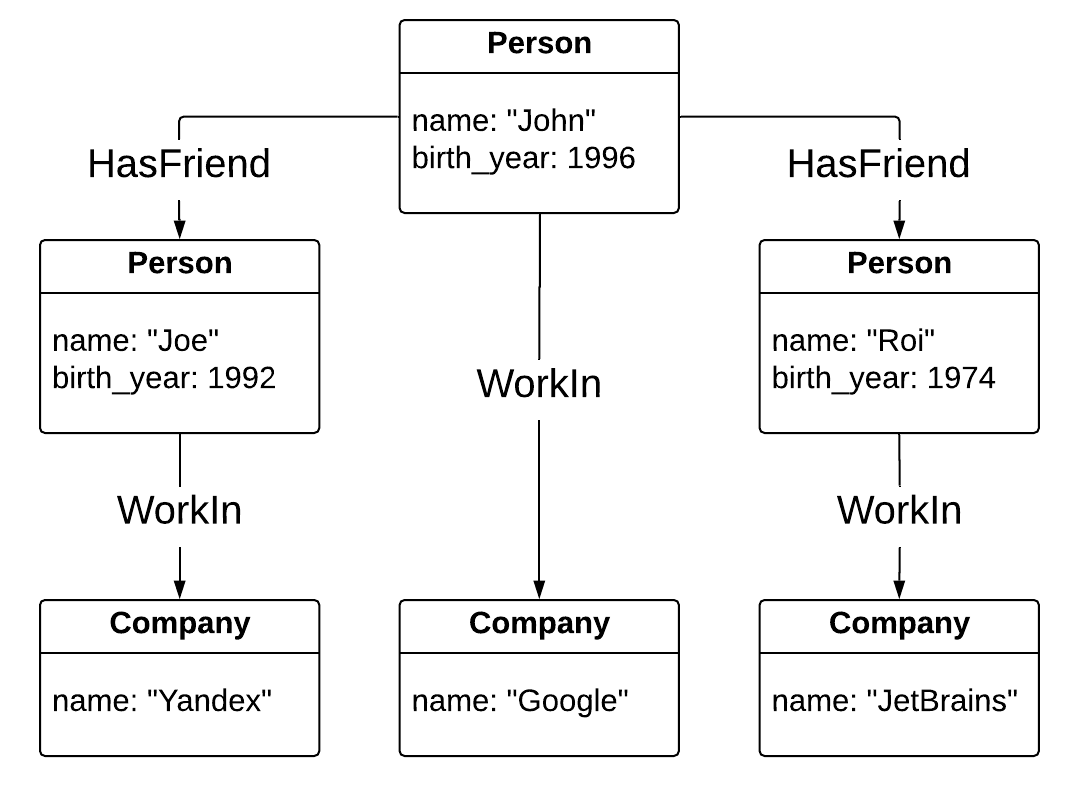
\includegraphics[width=0.7\linewidth]{Terekhov/pictures/graph_bd_1.png}
    \caption{Пример социального графа}
    \label{fig:graph_bd_1}
\end{figure}

Для работы с графами графовые базы данных предоставляют язык запросов, самым популярным из которых является Cypher~\cite{cypher-language}. В нём главный интерес представляют запросы вида сопоставления с образцом. Они позволяют задавать интересующие пути или подграфы в виде шаблонов и описывать информацию, которую нужно извлечь после удачного сопоставления. На рисунке~\ref{code:cypher_query} приведён пример такого запроса. Шаблон пути описывается в выражении MATCH. В нём между круглыми скобками задаются шаблоны вершин, а между квадратными шаблоны рёбер. Таким образом в данном примере задаются следующие ограничения: путь должен начинаться из вершины с меткой Person и именем John и состоять из двух рёбер, первое из которых должно иметь тип HasFriend, а второе WorkIn. В выражении RETURN задаётся информация, которую нужно извлечь. В данном примере это имя последней в пути вершины. В итоге ответом на такой запрос являются имена компаний, в которых работают друзья Джона. Результатом работы этого запроса на графе из рисунка~\ref{fig:graph_bd_1} является множество \{"Yandex", "JetBrains"\}.

%\lstset{
%   basicstyle=\fontsize{14}{14}\selectfont\ttfamily
%}

\begin{figure}[h]
\begin{lstlisting}[language=sql]
MATCH (p:Person)-[:HasFriend]->()-[:WorkIn]->(to)
WHERE p.name = "John"
RETURN to.name
\end{lstlisting}
\caption{Пример конечного запроса на языке Cypher}
\label{code:cypher_query}
\end{figure}

С формальной точки зрения шаблоны пути в выражении MATCH позволяют поставить задачу поиска путей с ограничениями в виде формальных языков. Так в запросе на рисунке~\ref{code:cypher_query} языком ограничений является конечный язык $\{(HasFriend, WorkIn)\}$. Для запроса на рисунке~\ref{code:cypher_query_2} ограничением является регулярный язык $\{A, B\}^*$. 

\begin{figure}[h]
\begin{lstlisting}[language=sql]
MATCH (v)-[:A | :B *]->(to)
RETURN to.name
\end{lstlisting}
\caption{Пример регулярного запроса на языке Cypher}
\label{code:cypher_query_2}
\end{figure}

При этом регулярные ограничения поддерживаются лишь частично и позволяют искать только пути произвольной длины с заданными метками на рёбрах, а более глубокие регулярные выражения не поддерживаются. Поэтому на текущий момент язык запросов довольно ограничен.

\subsection{Существующие решения}
Как было упомянуто раннее, ни одна графовая база данных не поддерживает запросов с контекстно-свободными ограничениями. Тем не менее существуют альтернативные решения поддержки таких запросов. 

\subsubsection{Парсер-комбинаторы для Neo4j}\label{sec:pareser-combinators}
В 2018 году группой исследователей из JetBrains Research на основе библиотеки Meerkat была разработана библиотека для поддержки запросов с контекстно-свободными ограничениями~\cite{parser-combinators}. Она использует графовую базу данных Neo4j~\cite{neo4j} как хранилище графов и позволяет задавать запросы в виде парсер-комбинаторов. Основным достоинством данной работы является то, что с помощью этой библиотеки кроме контекстно-свободных запросов можно выразить базовую часть языка Cypher. Но так как конкурировать с оригинальной реализацией выполнения запросов Neo4j очень сложно, это достигается вместе c сильной потерей производительности. Кроме этого контекстно-свободные запросы обрабатываются также достаточно медленно.

Таким образом данное решение является альтернативой языка запросов Neo4j, а не его расширением. Из-за медленного времени работы такое решение подходит только для работы с небольшими графами. 

\subsubsection{Расширение языка запросов SPARQL}\label{subsection:cypher-extention-2}
%Про sparql%
В 2016 Сяованг Чжан предоставил язык cfSPARQL~\cite{zhlang-2016} --- расширение языка SPARQL, который способен выразить запросы с контекстно-свободными ограничениями. Также он привёл алгоритм для вычисления таких запросов и замеры производительности. Но, во-первых, работа была сделана вне контекста графовой базы данных, а во-вторых, время работы предложенного алгоритма было больше, чем время работы парсер-комбинаторов.

\subsubsection{Существующие реализации алгоритмов решения задачи контекстно-свободной достижимости}
Основной сложностью расширения языка запросов для поддержки запросов с контекстно-свободными ограничениями является долгое время работы соответствующих алгоритмов. Так, например, в 2019 году Йохем Куйперс и другие исследователи с целью попытки расширения языка запросов Cypher для графовой базы данных Neo4j произвели сравнительный анализ производительности наиболее известных алгоритмов решения задачи контекстно-свободной достижимости.

В данном исследовании были рассмотрены и произведены замеры времени работы алгоритма Элле Хелингса~\cite{hellings-2015}, основанного на атрибутных грамматиках, восходящего алгоритма Фреда Сантоса~\cite{santos-2018}, матричного алгоритма Рустама Азимова~\cite{Azimov:2018:CPQ:3210259.3210264} и алгоритма Петтери Севона~\cite{bio-application}. Все алгоритмы были интегрированы в Neo4j и запускались на графах, находящихся в её хранилище. Алгоритмы были написаны на языке Java, при этом их реализация являлась однопоточной.

% \gsv{В таких местах надо сразу ссылку на алгоритм давать.}

По результатам замеров производительности было показано, что время работы алгоритмов является слишком большим и неприемлемым для широкого практического использования. Поэтому дальнейшая работа по интеграции и расширению языка запросов была приостановлена.

Тем не менее, матричный алгоритм Рустама Азимова в сравнительном анализе Йохема Куйперса был реализован без необходимых матричных библиотек, которые могут сильно уменьшить время его работы. Так, например, в исследовании Никиты Мишина и др.~\cite{azimov-evalution} был произведён сравнительный анализ времени работы нескольких реализаций алгоритма Рустама Азимова, основанных на различных специализированных матричных библиотеках. Графы и запросы к ним были взяты из объемлющего набора данных CFPQ\_Data~\cite{cfpq-data}, предоставленного лабораторией языковых инструментов JetBrains Research. 

Результаты замеров Никиты Мишина и др. показали, что при грамотной реализации алгоритма Рустама Азимова и использовании подходящих матричных библиотек можно добиться очень высокой производительности. Поэтому, так как основной проблемой применимости запросов с контекстно-свободными ограничениями является долгое время работы соответствующих алгоритмов, в качестве алгоритма решения задачи конте\-кстно-свободной достижимости был выбран матричный алгоритм Рустама Азимова.

\subsection{Матричный алгоритм Рустама Азимова}\label{sec:matrix-algo}
Выбранный в предыдущей главе алгоритм Рустама Азимова~\cite{Azimov:2018:CPQ:3210259.3210264}, в отличие от других алгоритмов решения задачи контекстно-свободной достижимости~\cite{hellings-2015, santos-2018, zhlang-2016}, работает с графами в виде разреженных матриц смежности. Данный алгоритм состоит из последовательности операций над разреженными матрицами, время работы которых зависит не от размеров матричных операндов, а от количества их ненулевых элементов.

На вход алгоритму (см. алгоритм 1) поступает помеченный граф $D=(V,E)$ и контекстно-свободная грамматика $G=(\Sigma, N, P, S)$ в ослабленной нормальной форме Хомского. Для каждого нетерминала $A$ в ассоциативном массиве $T$ хранится соответствующая ему булева матрица $T[A]$. На всём этапе алгоритма поддерживается следующий инвариант: $T[A]_{i,j} = 1$ равносильно существует пути, метки на рёбрах которого образуют слово, выводящееся из нетерминала $A$. На первом этапе происходит инициализация матриц с помощью простых правил грамматики, после чего инвариант выполняется для всех путей единичной длины. На втором этапе происходит транзитивное замыкание, после чего этот инвариант верен для всех путей. Результатом данного алгоритма является матрица, соответствующая стартовому нетерминалу $S$.

%  Это позволяет для его реализации использовать многопоточные матричные библиотеки, с помощью которых можно добиться очень высокой производительности. Поэтому на текущий момент алгоритм Рустама Азимова показывает наилучшее время работы на практике.

\begin{algorithm}
\caption{Матричный алгоритм Рустама Азимова}

\begin{algorithmic}[1]
\Function{contextFreePathQuerying}{$D$, $G$}
    \State{$n =$ getNodeCount(D)}
    \State{$N =$ getAllNonterms(G)}
    \State{$E =$ getEdges($D$)}
    \State{$P =$ getRules($G$)}
    \State{$S =$ getStartNonterm($G$)}
    \State{$T = \{A \rightarrow \varnothing_{n \times n} : A \in$ $N$ \} }
    \ForAll{$(v, to, label) \in E$}
    \Comment{Инициализация матриц}
        \ForAll{$A \rightarrow label \in P$}
            \State{$T[A]_{i,j} = 1$}
        \EndFor
    \EndFor    
    \While{$\exists A: T[A]$ is changing}
    \Comment{Вычисление замыкания}
        \ForAll{$A \rightarrow BC \in P$}
            \State{$T[A] \oplus= T[B] \otimes T[C]$}
        \EndFor
    \EndWhile
\State \Return $T[S]$
\EndFunction

\end{algorithmic}
\end{algorithm}

Практическое время работы алгоритма Рустама Азимова сильно зависит от производительности используемой матричной библиотеки. Это накладывает некоторые ограничения на выбор подходящей графовой базы данных, так же как и возможность представления графов в матричном виде.

\subsection{RedisGraph}
RedisGraph~\cite{redis-graph} --- это высокопроизводительная графовая база данных, поддерживающая язык запросов Cypher. В отличие от наиболее распространённой графовой базы данных Neo4j~\cite{neo4j}, RedisGraph написан на языке Си и для работы с данными использует Redis~\cite{redis}, основным достоинством которого является возможность хранить данные прямо в оперативной памяти. Это позволяет RedisGraph быстро обрабатывать пользовательские запросы.

Также RedisGraph является единственной графовой базой данных, которая работает с графами в виде разреженных матриц смежности и транслирует запросы языка Cypher в матричные выражения. Для представления графов в таком виде и работы с ними в терминах линейной алгебры используется мощный матричный фреймворк GraphBlas~\cite{graph-blas}. Его реализация SuiteSparse~\cite{suite-sparse} является многопоточной и сильно оптимизирована, что позволяет RedisGraph добиться высокой производительности.

Из всего этого следует, что RedisGraph идеально подходит для интеграции матричного алгоритма. Во-первых, графы представляются в необходимом алгоритму виде, что позволит избежать издержек на конвертацию форматов. Во-вторых, использование SuiteSparse для вычисления матричных операций позволит добиться высокой производительности. Поэтому RedisGraph был выбран в качестве графовой базы данных для интеграции матричного алгоритма и расширения языка запросов.

% Так как алгоритм Рустама Азимова работает с матричным представлением графа,, как наиболее подходящий для интеграции матричного алгоритма.

\subsection{Расширение языка Cypher}\label{subsection:cypher-extention}
На текущий момент оригинальная версия языка Cypher, используемая в том числе и в RedisGraph, не поддерживает запросов с контекстно-свободными ограничениями. Но тем не менее в 2017 году был разработан черновой вариант спецификации расширения Cypher~\cite{cypher-specification}, которая вводит в язык шаблоны путей. Они позволяют выразить более сложные запросы, в том числе запросы с контекстно-свободными ограничениями.

Шаблоны путей являются альтернативой шаблонам рёбер, которые есть в оригинальном Cypher. Они, как и шаблоны рёбер, могут встречаться в выражении MATCH и иметь своё направление. Кроме этого в глобальной области запроса им можно задавать имя, на которое потом можно ссылаться внутри других шаблонов.

Шаблон пути представляет из себя регулярное выражение над некоторыми примитивами. В качестве таких примитивов могут выступать шаблоны рёбер, шаблоны вершин и ссылки на именованные шаблоны путей. Также любым подвыражениям можно задавать своё направление. Основная часть конкретного синтаксиса данного расширения приведена на рисунке~\ref{fig:cypher_syntax}.

\begin{figure}[]
\begin{align*}
\begin{split}
PathPattern     &= ["<"],~"-/",~PathExpression,~"/-",~[">"]\\
PathExpression  &= \{PathAlternative\}\\
PathAlternative &= PathRepetition,~\{"|", PathRepetition\}\\
PathRepetition  &= ["<"],~PathBase,~[">"],~("*")
\end{split}\\
\begin{split}
PathBase &= PathEdge \\
         &~~|~PathNode \\
         &~~|~PathReference \\
         &~~|~"[",~PathExpression,~"]"
\end{split}\\
\begin{split}
PathEdge      &= Label \\
PathNode      &= "(",~[Label,~\{"|",~Label\}],~")" \\
PathReference &= "\sim",~SymbolicName; \\
Label         &= ":",~LabelName
\end{split}
\end{align*}
\caption{Расширение конкретного синтаксиса Cypher}
\label{fig:cypher_syntax}
\end{figure}

Каждый шаблон пути задаёт отношение на множестве вершин. Поэтому семантикой языка шаблонов путей $L_{P}$ в контексте графа $G(V, E)$ является отображение $\llbracket \cdot \rrbracket_{G}: L_P \rightarrow V \times V$, которое каждому шаблону $p\in L_P$ сопоставляет множество пар вершин, между которыми существует путь, удовлетворяющий данному шаблону $p$. 

Подробное описание данной семантики приводится в таблице~\ref{tab:cypher_sematic}.  В ней наибольший интерес представляют именованные шаблоны путей, так как именно с помощью них можно выразить запросы с контекстно-свободными ограничениями. Все именованные шаблоны путей $S_i = p_j$ можно рассматривать как правила контекстно свободной грамматики с алфавитом нетерминалов $\{S_i\}_{i=1}^n$. Тогда каждый нетерминал $S_j$ порождает язык $L_{S_j} \subset L_p$, а семантикой соответствующего именованного шаблона пути $S_j=p_j$ является множество $\bigcup\limits_{p \in L_{s_j}} \llbracket p \rrbracket_{G}$.

На рисунке~\ref{code:cypher_query_3} приведён пример запроса в расширенном синтаксисе. В нём декларируется именованный шаблон S, который задаёт множество правильных скобочных последовательностей над ребрами с типом L и R. Далее в выражении MATCH задаётся шаблон пути, состоящий из ссылки на шаблон S. Таким образом результатом обработки запроса является множество всех пар вершин, между которыми существует путь, метки на рёбрах которого образуют правильную скобочную последовательность. 

\begin{table}[h!]
\begin{adjustbox}{max width=\textwidth}
\begin{tabular}{|c|c|c|}
\hline
$p \in L_P$                                                                                  & $\llbracket p \rrbracket_{G}$                                                                                                                                                                                   & Описание шаблона пути                                                                                                         \\ \hline
\hline
()                                                                                            & $\{(v, v): v \in V\}$                                                                                                                                                                                           & \begin{tabular}[c]{@{}c@{}}Пустой путь, состоящий из \\ одной произвольной вершины\end{tabular}                               \\ \hline
:a                                                                                            & $\{e=(v,to): e \in E, type(e)=a\}$                                                                                                                                                                              & \begin{tabular}[c]{@{}c@{}}Путь единичной длины,\\  состоящий из ребра с типом $a$\end{tabular}                               \\ \hline
(:b)                                                                                          & $\{(v, v): v \in V, label(v)=b\}$                                                                                                                                                                               & \begin{tabular}[c]{@{}c@{}}Пустой путь, состоящий из одной\\  вершины, помеченной меткой $b$\end{tabular}                     \\ \hline
$\alpha~\beta$                                                                                & $\llbracket \alpha \rrbracket_{G}\circ \llbracket \beta \rrbracket_{G}$                                                                                                                                         & Конкатенация путей $\alpha$ и $\beta$                                                                                         \\ \hline
$\alpha~|~\beta$                                                                              & $\llbracket \alpha \rrbracket_{G}\cup \llbracket \beta \rrbracket_{G}$                                                                                                                                          & Альтренатива между путями $\alpha$ и $\beta$                                                                                  \\ \hline
$[\alpha]$                                                                                    & $\llbracket \alpha \rrbracket_{G}$                                                                                                                                                                              & \begin{tabular}[c]{@{}c@{}}Квадратные скобки позволяют \\ группировать  выражения \\ для задания ассоциативности\end{tabular} \\ \hline
\textless{}$\alpha$                                                                           & $\{(to, v): (v, to) \in \llbracket \alpha \rrbracket_{G}\}$                                                                                                                                                     & Путь, обратный к пути $\alpha$                                                                                                \\ \hline
\textless{}$\alpha$\textgreater{}                                                             & $\llbracket \alpha~|~$\textless{}$\alpha \rrbracket_{G} $                                                                                                                                                       & \begin{tabular}[c]{@{}c@{}}Альтернатива между путём $\alpha$ и\\ обратным к нему\end{tabular}                                 \\ \hline
$\alpha^*$                                                                                    & $\llbracket \alpha \rrbracket_{G}^{*}$                                                                                                                                                                          & \begin{tabular}[c]{@{}c@{}}Путь, состоящий из\\ конкатенации 0 или более путей $\alpha$\end{tabular}                          \\ \hline
\begin{tabular}[c]{@{}c@{}}$\{S_i = p_i\}_{i=1}^{n}$\\ -- named\\  path patterns\end{tabular} & \begin{tabular}[c]{@{}c@{}}$P = \{S_i \rightarrow p_i\}_{i=1}^n$\\ $Gram_j = (\Sigma, \{S_i\}_{i=1}^n, P, S_j)$\\ $\llbracket S_j \rrbracket_{G} = \bigcup\limits_{p \in L(G)}{\llbracket p \rrbracket_{G}}$\end{tabular} & Именнованые шалоны путей                                                                                                      \\ \hline
$\sim$$S$                                                                                     & $\llbracket S \rrbracket_{G}$                                                                                                                                                                                   & \begin{tabular}[c]{@{}c@{}}Ссылка на именнованный\\  шаблон пути\end{tabular}                                                 \\ \hline
\end{tabular}
\end{adjustbox}
\caption{Семантика языка шаблонов путей}
\label{tab:cypher_sematic}
\end{table}

\begin{figure}[h!]
\begin{lstlisting}[language=sql]
PATH PATTERN S = ()-/ [:L ~S :R] | [~S ~S] | () /-()
MATCH (v)-/ ~S /-(to)
RETURN v, to
\end{lstlisting}
\caption{Пример запроса в расширенном синтаксисе Cypher}
\label{code:cypher_query_3}
\end{figure}

Данная спецификация расширения Cypher была представлена официальными разработчиками и сильно расширяет выразительность языка, предоставляя удобную возможность выражать запросы как с регулярными, так и с контекстно-свободными ограничениями. Поэтому в моей работе приводится поддержка выполнения запросов именно для этого расширения языка.

% \gsv{Не хватает какого-то чёткого вывода про то, что вот именно это мы и буем использовать.}

\section{Реализация}
По результатам обзора было решено реализовать поддержку расширения языка Cypher, представленную в главе~\ref{subsection:cypher-extention}, для графовой базы данных RedisGraph. За основу алгоритма, решающего задачу поиска путей с контекстно-свободными ограничениями, был взят матричный алгоритм Рустама Азимова, описанный в главе~\ref{sec:matrix-algo}.

% \gsv{И зжесь надо ещё раз подитожить в духе "по результатм обзора было решено сделать то и это с использованием того и сего"}

\subsection{План выполнения запроса}\label{execution-plan}
В RedisGraph основной частью обработки запроса является построение плана его выполнения. Её часть, которая относится к шаблонам путей приведена на рисунке~\ref{fig:execution_plan}. В ней зелёным цветом выделено то, что было добавлено или расширено.

В самом начале, после получения запроса строится его абстрактное синтаксическое дерево \textit{AST}. Далее, из него извлекаются именованные и неименованные шаблоны путей \textit{PathPattern} и \textit{NamedPathPatterns}, после чего они преобразуются в более удобное промежуточное представление \textit{PathExpr}. При этом, для дальнейшего связывания ссылок, именованные шаблоны сохраняются в глобальном контексте запроса \textit{PathPatternCtx}.

На следующем этапе происходит трансляция промежуточных представлений \textit{PathExpr} в матричные выражения \textit{AlgebraicExpression}. В них операндами являются либо матрицы, полученные из указанного в запросе графа \textit{GraphCtx}, либо ссылки на именованные шаблоны путей из \textit{PathPatternCtx}. Основной идеей трансляции является то, что после вычисления матричного выражения получается матрица, которая задаёт то же самое отношение на множестве вершин, что и исходный шаблон пути.

Далее каждое такое выражение формирует новую операцию плана выполнения запроса \textit{CfpqTraverseOp}. При её вычислении сначала происходит запуск расширенной версии матричного алгоритма Рустама Азимова. Он решает задачу контекстно-свободной достижимости, заданной именованными шаблонами путей. После этого все ссылки в матричном выражении заменяются на полученные в ходе алгоритма матрицы и происходит вычисление матричного выражения. Каждая такая операция добавляется в план выполнения запроса.

%  \gsv{Используйте \textit{CfpqTraverseOp} вместо долларов для длинных слов. Они тогда не распадаются из-а лишних пробелов.}

\begin{figure}[H]
\centering
    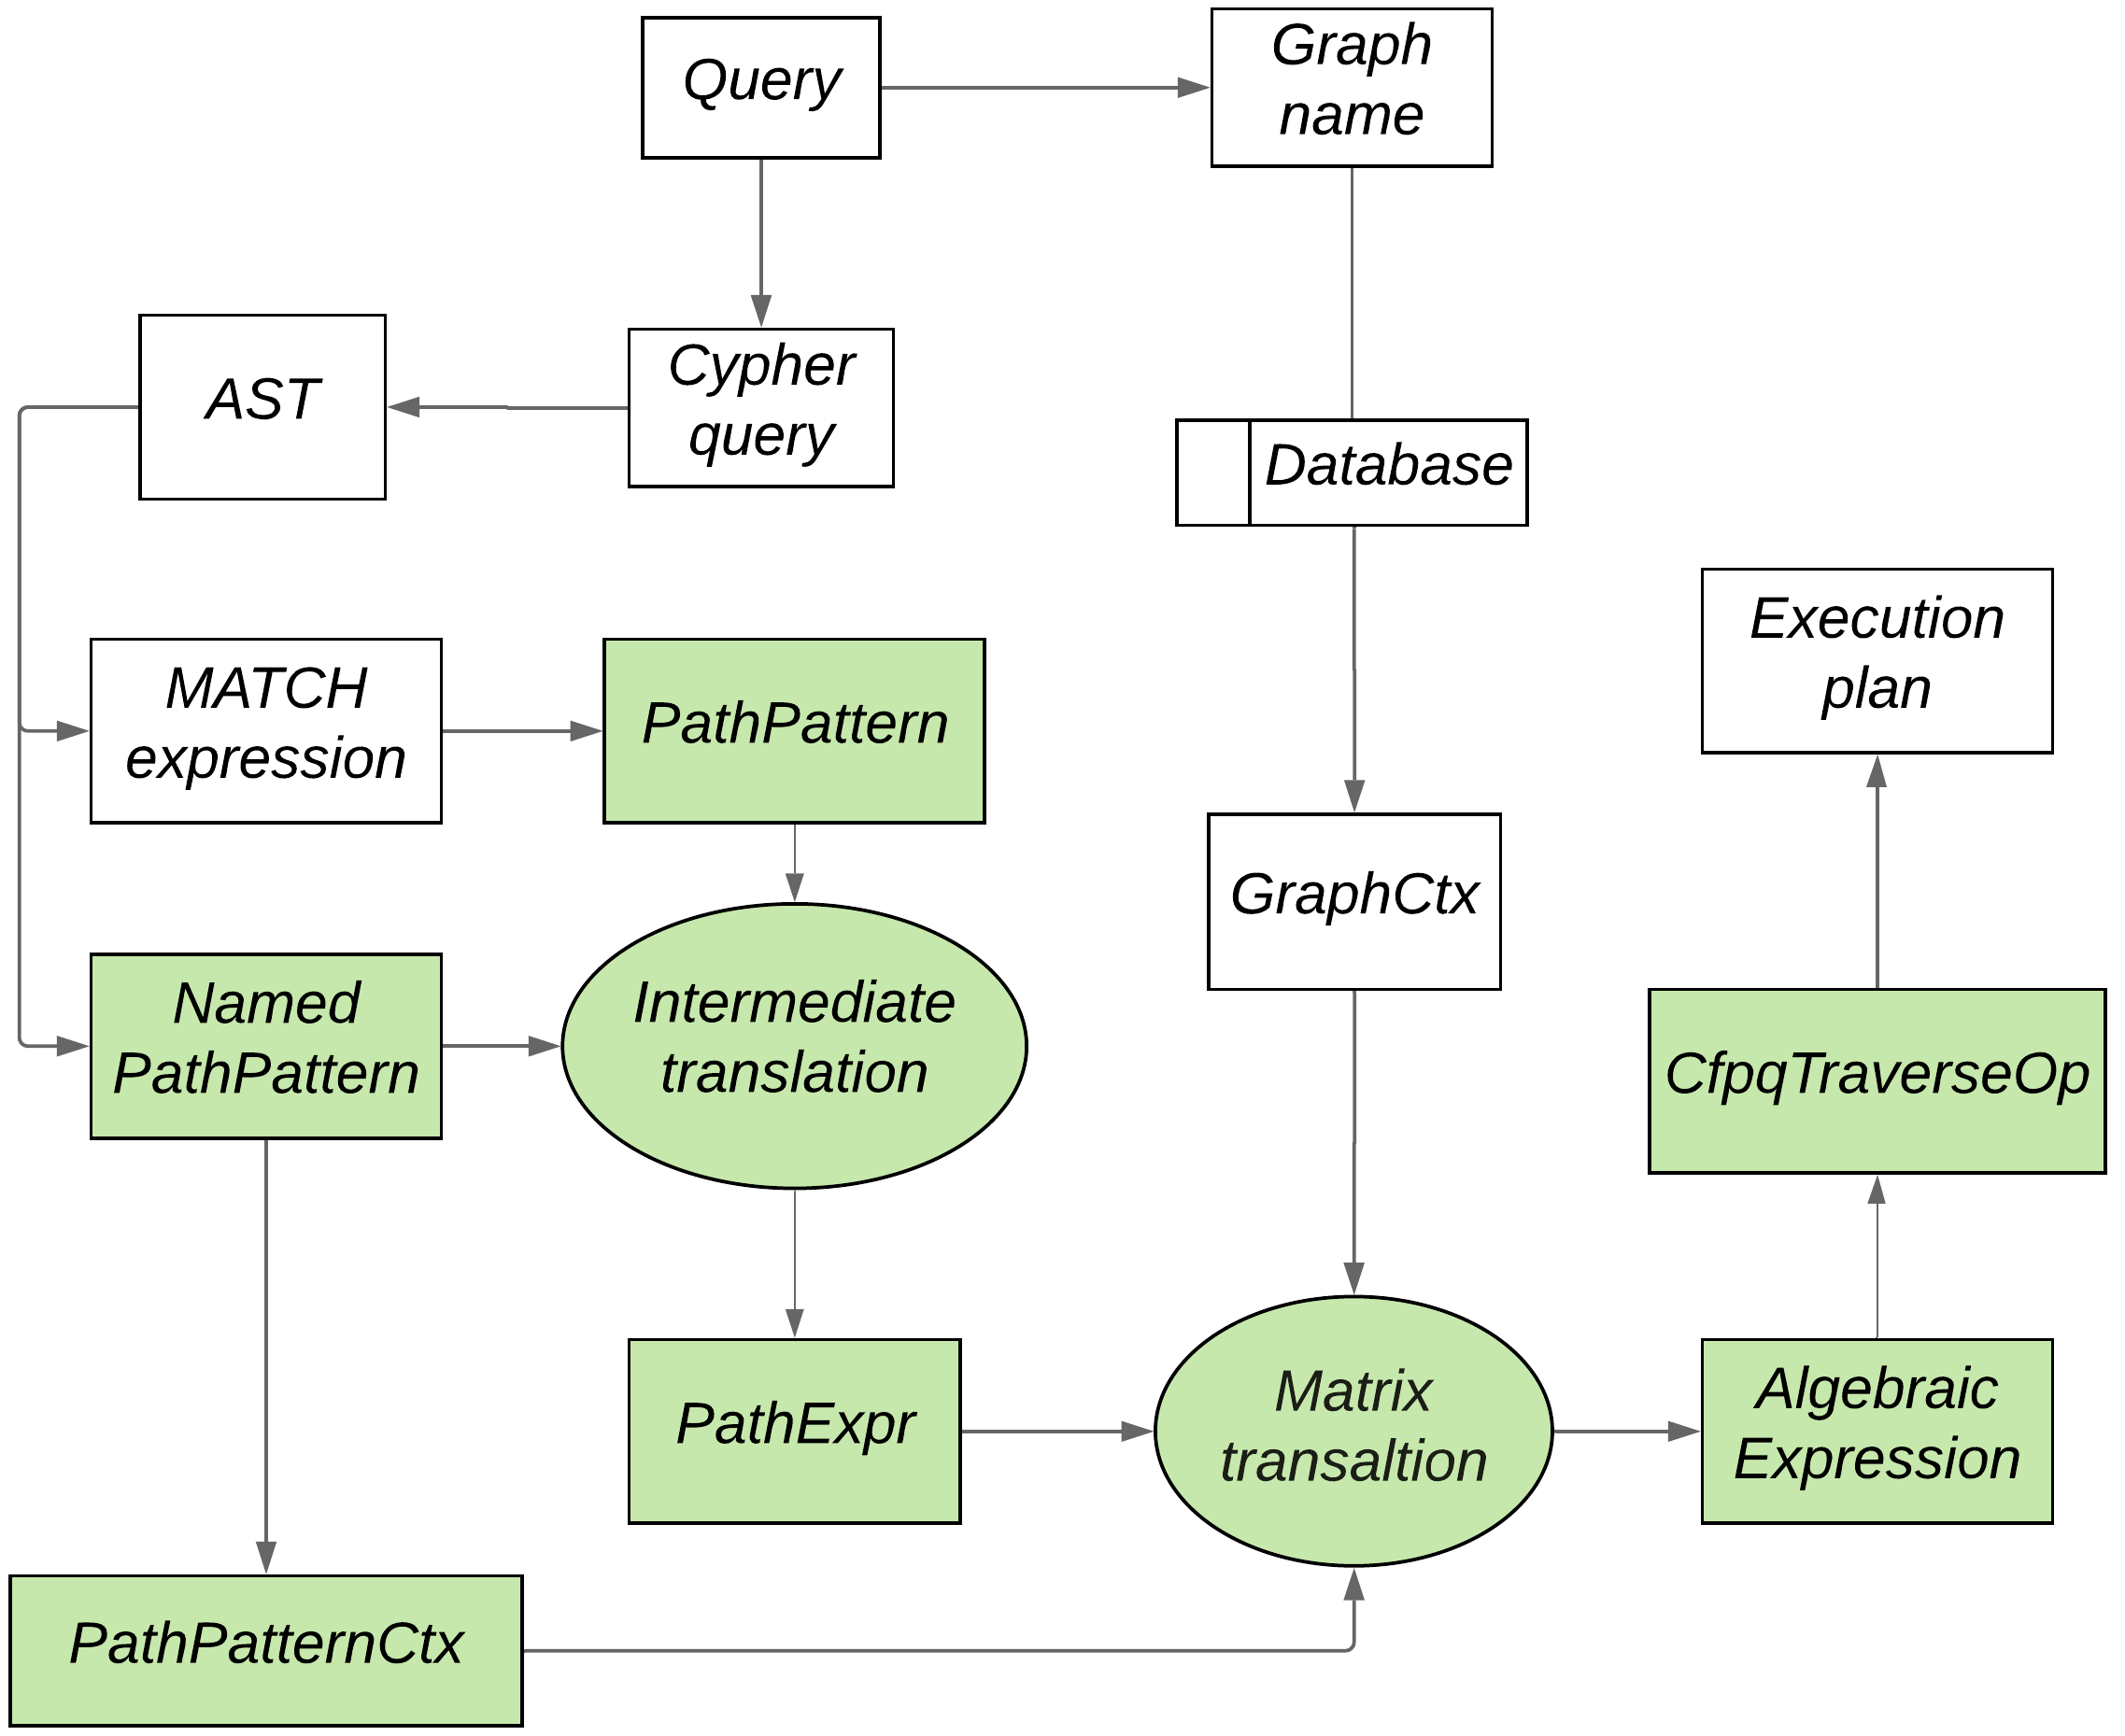
\includegraphics[width=1.0\linewidth]{Terekhov/pictures/execution_plan_3.png}
    \caption{Расширение построения плана выполнения запроса}
    \label{fig:execution_plan}
\end{figure}

\subsection{Промежуточное представление}\label{matrix-translation}
Шаблоны путей, полученные из \textit{AST}, транслируются в промежуточное представление \textit{PathExpr}. Оно позволяет задавать более простой абстрактный синтаксис, который описан на рисунке~\ref{fig:intermidiate_repr}. 

Таким образом, альтернативе и конкатенации шаблонов соответствуют \textit{PathAlt} и \textit{PathSeq}, \textit{PathGroup} позволяет задавать направление пути и наличие замыкания, а \textit{PathBasic} соответствует либо примитивным шаблонам \textit{PathNode}, \textit{PathEdge} и \textit{PathRef}, либо целому выражению \textit{PathExpr}. Примеры промежуточного представления шаблонов приведены в таблице~\ref{tab:inter_examples}.
\begin{figure}[h!]
\begin{align*}
\begin{split}
PathExpr=~ &PathSeq(PathExpr,~PathExpr)~|\\
           &PathAlt(PathExpr,~PathExpr)~|\\
           &PathGroup(PathBasic, direction, range)
\end{split}\\
\begin{split}
PathBasic=~ &PathNode(label)~|\\
            &PathEdge(type)~~|\\
            &PathRef(name) ~~|\\
            &PathExpr
\end{split}\\
\begin{split}
direction \in ~&\{inbound,~outbound,~bidirectional\}\\
range \in     ~&\{*, \varnothing\}
\end{split}
\end{align*}
\caption{Промежуточное представление PathExpr}
\label{fig:intermidiate_repr}
\end{figure}

\begin{table}[h]
\centering
\begin{adjustbox}{max width=\textwidth}
\begin{tabular}{|c|l|}
\hline
$L_p$                        & \multicolumn{1}{c|}{PathExpr}                                                                                                        \\ \hline
{[}:A :B{]} | (:C)           & \begin{tabular}[c]{@{}l@{}}$PathAlt($\\ $~~~~PathSeq(PathEdge("A"),~PathEdge("B"))$\\ $~~~~PathNode("C")$\\ $)$\end{tabular}         \\ \hline
\textless{}{[}:A $\sim$S{]}* & \begin{tabular}[c]{@{}l@{}}$PathGroup($\\ $~~~~PathSeq(PathEdge("A"),~PathRef("S")),$\\ $~~~~inbound,$\\ $~~~~*,$\\ $)$\end{tabular} \\ \hline
\end{tabular}
\end{adjustbox}
\caption{Примеры промежуточного представления запросов}
\label{tab:inter_examples}
\end{table}

\newpage
\subsection{Трансляция в матричные выражения}
Как было упомянуто ранее, RedisGraph представляет графы в виде разреженных матриц. А именно каждый граф $G$ задаётся следующей тройкой $(A \in M_{n\times n},~lab \in Labels \rightarrow Diag_n,~rel \in RelTypes \rightarrow M_{n \times n})_G$. Здесь $M_{n \times n}$ означает полукольцо булевых матриц, а $Diag_n$ полукольцо диагональных булевых матриц. Матрица $A$ служит матрицей смежности графа, а отображения $lab$ и $rel$ сопоставляют меткам вершин и типам рёбер соответствующие булевы матрицы. Таким образом, ребро $(v, to)$ графа $G$ имеет тип $a$ тогда и только тогда, когда $rel(a)_{v,to} = 1$.  Таким же образом, принадлежность метки $l$ вершине $v$ равносильно $lab(l)_{v,v}=1$.

Любую булеву матрицу $M$, участвующую в задании графа $G(V, E)$, можно рассматривать как отношение на множестве вершин $R(M) = \{(v, to):~M_{v,to}=1\}$. Операциями сложения и умножения в булевом полукольце являются дизъюнкция и конъюнкция. Поэтому умножению матриц $A*B$ соответствует композиция отношений $R(A) \circ R(B)$, сложению $A+B$ соответствует объединение отношений $R(A) \cup R(B)$, а транспонированная матрица $A^T$ соответствует обратному к R(A) отношению $R(A)^{-1}$. Такая взаимосвязь между матричными операциями и отношениями лежит в основе алгоритма трансляции, приведённом на рисунке~\ref{algo:translation}.

Данный алгоритм является рекурсивным и принимает на вход промежуточное представление шаблона пути $expr$, представление графа $g$ и контекст именованных шаблонов путей $pathCtx$. Целевым языком трансляции является простой язык матричных выражений, приведённый на рисунке~\ref{fig:alg-expr}.

Базовым случаем рекурсии являются примитивные шаблоны \textit{Path\-Node}, \textit{PathEdge} и \textit{PathReference}, которые транслируются в операнды матричного выражения. Для первых двух соответствующие матрицы извлекаются из графа с помощью функций \textit{GetLabel\-Matrix} и \textit{GetRelation\-Matrix}. При этом случай $label = \varnothing$ соответствует шаблону пути, состоящему из одной произвольной вершины. Поэтому такой путь задаётся тождественным отношением $R(I)$, где $I$ --- единичная матрица. Для \textit{Path\-Reference} создаётся ссылка на матрицу именованного шаблона, которая будет вычислена на следующем этапе при выполнении алгоритма контекстно-свободной достижимости.

Трансляция для шаблонов \textit{PathSeq} и \textit{PathAlt} происходит одинаковым образом --- сначала происходит трансляция дочерних шаблонов, а потом из полученного результата образуются операции умножения или сложения. Такая трансляция обосновывается семантикой шаблонов альтернативы и конкатенации, приведенной в главе~\ref{subsection:cypher-extention}, и связью отношений с матричными операциями, описанными раннее.

Наиболее интересным случаем является трансляция \textit{Path\-Group}, так как в некоторых случаях контекст именованных шаблонов $pathCtx$ расширяется. В начале происходит трансляция дочернего шаблона. Далее, если заданное направление является обратным, к полученной матрице применяется операция транспонирования. Если же направление является произвольным, то формируется операция сложения из полученной матрицы и транспонированной к ней. Это соответствует альтернативе между прямым путём и обратным к нему. После этого при отсутствии замыкания результат возвращается. Иначе происходит трансляция замыкания полученного выражения. Так как его нельзя выразить через имеющиеся матричные операции, создаётся новый именованный шаблон, а замыкание заменяется ссылкой на него. Нетрудно показать, что регулярное выражение $R^*$ и контекстно-свободная грамматика с одним правилом $S \rightarrow R~S \mid \epsilon$ равносильны. Поэтому правая часть этого правила тривиальным образом сразу же транслируется в выражение \textit{Add(Mul(R, MatrixRef(S)), I)} и добавляется в \textit{pathCtx} вместе с полученным новым именем.

Таким образом, после работы данного алгоритма из промежуточного представления шаблона пути получается выражение над матрицами. При дальнейшем его вычислении получается матрица, которая соответствует такому же отношению на множестве вершин, как и семантика изначального шаблона.

\algnewcommand\algorithmicswitch{\textbf{switch}}
\algnewcommand\algorithmiccase{\textbf{case}}
\algnewcommand\algorithmicof{\textbf{of}}
\algnewcommand\algorithmicassert{\texttt{assert}}
\algnewcommand\algorithmiccasepart{\texttt{:}}
\algnewcommand\Assert[1]{\State \algorithmicassert(#1)}%
% New "environments"
\algdef{SE}[SWITCH]{Switch}{EndSwitch}[1]{\algorithmicswitch\ #1}{\algorithmicend\ \algorithmicswitch}%
\algdef{SE}[CASE]{Case}{EndCase}[1]{\algorithmiccase\ #1\algorithmiccasepart}{\algorithmicend\ \algorithmiccase}%
\algdef{SE}[CASEPART]{CasePart}{EndCasePart}[1]{#1\algorithmiccasepart}{\algorithmicend\ \algorithmiccasepart}%
\algtext*{EndSwitch}%
\algtext*{EndCase}%
\algtext*{EndCasePart}%

\begin{algorithm}
\caption{Алгоритм трансляции}
\begin{algorithmic}[1]
\Function{translate}{PathExpr expr, GraphCtx g, PathPatternCtx pathCtx}
    \Switch{expr}
        \Case{$PathNode$(label)}
            \If{label $== \varnothing$}
                \State \Return \Call{GetIdentityMatrix}{g}
            \Else
                \State \Return \Call{GetLabelMatrix}{g, label}
            \EndIf
        \EndCase
        \Case{$PathEdge$(type)}
            \State \Return \Call{GetRelationMatrix}{g, type}
        \EndCase
        \Case{$PathRef(name)$}
            \State \Return $MatrixRef$(name)
        \EndCase
        \Case{$PathSeq$(left, right)}
            \State \Return Add(\Call{translate}{left}, \Call{translate}{right})
        \EndCase
        \Case{$PathAlt$(left, right)}
            \State \Return Mul(\Call{translate}{left}, \Call{translate}{right})
        \EndCase
        \Case{$PathGroup$(basic, dir, range)}
            \State res = \Call{translte}{basic}
            \Switch{dir}
                \Case{$inbound$}
                    \State res = $Transpose$(res)
                \EndCase
                \Case{$bidirectional$}
                    \State res = $Add$(res, $Transpose$(res))
                \EndCase
            \EndSwitch
            \Switch{range}
                \Case{ $\varnothing$}
                    \State \Return res
                \EndCase
                \Case{$*$}
                    \State name = \Call{AllocateNewPathPattern}{ctx}
                    \State res = $Mul$(res, $MatrixRef$(name))
                    \State res = $Add$(res, \Call{GetIdentityMatrix}{g})
                    \State \Call{SetPathPetternExpression}{p, name, res}
                    \State \Return $MatrixRef$(name)
                \EndCase
            \EndSwitch
        \EndCase
    \EndSwitch
\EndFunction
\end{algorithmic}
\caption{Алгоритм транслции в матричные выражения}
\label{algo:translation}
\end{algorithm}

\begin{figure}[H]
\begin{align*}
\begin{split}
AlgExpr= ~ &Add(AlgExpr, AlgExpr)~|\\
           &Mul(AlgExpr, AlgExpr)~|\\
           &Transpose(AlgExpr)~|\\
           &Matrix~|\\
           &MatrixRef(ref)
\end{split}
\end{align*}
\caption{Алгебраическое выражение над матрицами}
\label{fig:alg-expr}
\end{figure}

\subsection{Формирование и вычисление операции плана выполнения}
После этапа трансляции в RedisGraph происходит построение плана выполнения запроса. Он формируется из последовательности операций, которые выполняют базовые вычисления. Для поддержки шаблонов путей была добавлена операция \textit{CfpqTraverseOp}. Она создаётся для каждого матричного выражения, полученного на предыдущем шаге из неименованого шаблона пути, и отвечает за его вычисление.

На этапе инициализации новой операции \textit{CfpqTraverseOp} из соответствующего матричного выражения рекурсивно извлекаются все ссылки на именованные шаблоны путей, от которых зависит данное выражение. После этого они поступают на вход алгоритма, решающего задачу контекстно-свободной достижимости (см. алгоритм 4).

Этот алгоритм является расширенной версией матричного алгоритма Рустама Азимова, приведенного в главе~\ref{sec:matrix-algo}. В данном алгоритме, в отличие от алгоритма Рустама Азимова, не требуется задавать правила грамматики в ослабленной нормальной форме Хомского. Вместо этого правая часть правила задаётся с помощью промежуточного представления \textit{PathExpr}. При этом подразумевается, что для любого именованного шаблона $p$ из глобального контекста \textit{pathCtx} его промежуточное представление уже транслировано в матричное выражение и записано в \textit{pathCtx[p].algExpr}.

Принцип работы алгоритма остаётся прежним. На каждой итерации для всех невычисленных шаблонов происходит вычисление матричного выражения. Если результирующая матрица не изменяется, то она является окончательной для данного именованного шаблона и он больше не участвует в обновлении. Иначе соответствующая матрица перезаписывается.

После работы данного алгоритма все ссылки на именованные шаблоны путей в матричном выражении заменяются на подсчитанные алгоритмом матрицы, после чего происходит вычисление матричного выражения. Результат сохраняется в операции $CfpqTraverseOp$ и участвует в вычислении плана выполнения запроса наряду с результатами других операций. 
\begin{algorithm}
\begin{algorithmic}[1]
\Function{CfpqTraverseNew}{String[] patterns, PathPatternCtx pathCtx}
\While{$\exists$ p $\in$ patterns: !pathCtx[p].isEvaluated}
    \ForAll{p $\in$ patterns}
        \If{!pathCtx[p].isEvaluated}
            \State new\_matrix = \Call{EvalueteAlgExpr}{pathCtx[p].expr}
            \If{new\_matrix == pathCtx[p].matrix}
                \State pathCtx[p].isEvaluated = true
            \Else
                \State pathCtx[p].matrix = new\_matrix
            \EndIf
        \EndIf
    \EndFor
\EndWhile
\EndFunction
\end{algorithmic}
\label{algo:matrix-extention}
\caption{Расширенный матричный алгоритм}
\end{algorithm}


\section{Замеры производительности}
После реализации поддержки нового синтаксиса шаблонов путей были произведены замеры производительности.

\subsection{Сравнение с парсер-комбинаторами}\label{sec:parse-comp-compare}
Сравнительный анализ времени работы полученного решения (колонка RedisGraph) и библиотеки парсер-комбинаторов (колонка Meer\-kat), описанной в главе~\ref{sec:pareser-combinators}, приведён в таблице~\ref{tab:combinators-vs-redisgraph}. Запросы были взяты из эксперимента оригинальной статьи про парсер-комбинаторы~\cite{parser-combinators}. Эквивалентные им запросы, написанные в расширенном синтаксисе Cyp\-her, приведены на рисунках~\ref{code:sub_clas_of_1},~\ref{code:sub_clas_of_2} и представляют из себя частный случай запросов поиска объектов, лежащих на одном уровне иерархии. Набор графов также был взят из вышеупомянутого эксперимента и впервые был представлен в статье Сяованга Чжана~\cite{zhlang-2016}.

% \gsv{У Вас в тексте минимум два разных варианта написания названия этой библиотеки. Надо бы узнать, как правильно и унифицировать}
% \gsv{ лежащих на одном уровне в иерархии}

Замеры обоих решений производились локально на оборудовании со следующими характеристиками: Intel Core i7 4$\times$1.8GHz, 8 GB RAM. Каждый запрос запускался 20 раз и время его работы усреднялось. Время работы указано в миллисекундах. Также в колонках $|V|$ и $|E|$ указано количество вершин и рёбер графа, а в колонке $\#result$ количество найденных соответствующим запросом пар вершин. 

\begin{table}[h!]
\begin{adjustbox}{max width=\textwidth}
\begin{tabular}{|l|c|c|c|c|c|c|c|c|}
\hline
\multicolumn{1}{|c|}{\multirow{2}{*}{$G$}}                   & \multirow{2}{*}{$|V|$} & \multirow{2}{*}{$|E|$} & \multicolumn{3}{c|}{Query\_1}                                                                                                           & \multicolumn{3}{c|}{Query\_2}                                                                                                           \\ \cline{4-9} 
\multicolumn{1}{|c|}{}                                       &                        &                        & \#result & \begin{tabular}[c]{@{}c@{}}Meerkat\\ time (ms)\end{tabular} & \begin{tabular}[c]{@{}c@{}}RedisGraph\\ time (ms)\end{tabular} & \#result & \begin{tabular}[c]{@{}c@{}}Meerkat\\ time (ms)\end{tabular} & \begin{tabular}[c]{@{}c@{}}RedisGraph\\ time (ms)\end{tabular} \\ \hline
wine                                                         & 773                    & 2450                   & 66572    & 541                                                         & 31                                                             & 133      & 6                                                           & 3                                                              \\ \hline
pizza                                                        & 671                    & 2604                   & 56195    & 476                                                         & 24                                                             & 1262     & 30                                                          & 4                                                              \\ \hline
\begin{tabular}[c]{@{}l@{}}measure-\\ primitive\end{tabular} & 341                    & 771                    & 15156    & 158                                                         & 11                                                             & 2871     & 39                                                          & 5                                                              \\ \hline
funding                                                      & 778                    & 1480                   & 17634    & 99                                                          & 14                                                             & 1158     & 14                                                          & 6                                                              \\ \hline
\begin{tabular}[c]{@{}l@{}}atom-\\ primitive\end{tabular}    & 291                    & 685                    & 15454    & 102                                                         & 10                                                             & 122      & 53                                                          & 3                                                              \\ \hline
\begin{tabular}[c]{@{}l@{}}people-\\ pets\end{tabular}       & 337                    & 834                    & 9472     & 55                                                          & 7                                                              & 37       & 3                                                           & 3                                                              \\ \hline
travel                                                       & 131                    & 397                    & 2449     & 21                                                          & 3                                                              & 63       & 2                                                           & 2                                                              \\ \hline
\end{tabular}
\end{adjustbox}
\caption{Сравнение Meerkat и полученного решения}
\label{tab:combinators-vs-redisgraph}
\end{table}

\begin{figure}[h!]
\begin{adjustbox}{max width=\textwidth}
\begin{lstlisting}[language=sql]
PATH PATTERN S = ()-/ [<:Type     [~S | ()] :Type] | 
                      [<:SubClass [~S | ()] :SubClass] /-()
MATCH (v)-/ ~S /->(to)
RETURN COUNT(*)
\end{lstlisting}
\end{adjustbox}
\caption{Query\_1}
\label{code:sub_clas_of_1}
\end{figure}

\begin{figure}[h!]
\begin{adjustbox}{max width=\textwidth}
\begin{lstlisting}[language=sql]
PATH PATTERN S = ()-/ :SubClass | [<:SubClass ~S :SubClass] /-()
MATCH (v)-/ ~S /->(to)
RETURN COUNT(*)
\end{lstlisting}
\end{adjustbox}
\caption{Query\_2}
\label{code:sub_clas_of_2}
\end{figure}

По результатам замеров видно, что даже на небольших графах время работы Meerkat сильно больше, чем время работы полученного решения. При этом в большинстве случаев оно отличатся на порядок. Также стоит отметить, что запросы, указанные на рисунках~\ref{code:sub_clas_of_1},~\ref{code:sub_clas_of_2}, помимо расширенного синтаксиса используют и оригинальную часть языка Cyp\-her, а конкретно функцию COUNT. Это является небольшим примером того, что расширение языка запросов является полностью совместимым с его оригинальной частью.

% Эксперимент, проведенный в статье про парсер-комбинаторы, описанные в  был повторён локально на оборудовании с характеристиками.
% Каждое матричное выражение, полученное при трансляции шаблонов путей, формирует операцию плана выполнения запроса $CfpqTraverse$.

\subsection{Сравнение с матричным алгоритмом}
Графы, приведенные в предыдущих замерах являются достаточно маленькими, поэтому также были произведены замеры на более больших графах. Они были взяты из набора данных CFPQ\_Data~\cite{cfpq-data}, собранного исследователями лаборатории языков инструментов JetBrains Research. Замеры производились таким же образом и на том же оборудовании, что и в главе~\ref{sec:parse-comp-compare}.

% \gsv{Кажется, что нет. go  и прочие большие графы уже просто из нашего набора данных CFPQ\_Data, у китайцев их не было.}

Кроме этого, для анализа издержек выполнения запроса в таблице~\ref{tab:combinators_vs_redisgraph} приводится время работы оригинального алгоритма Рустама Азимова (колонка Matrix algorithm), описанного в главе~\ref{sec:matrix-algo}. Данный алгоритм был интегрирован в RedisGraph и запускался на графах, находящихся в его хранилище. Для этого была разработана отдельная команда, принимающая на вход название графа и путь до файла с грамматикой, написанной в нормальной форме Хомского. Для вычисления матричных операций также использовалась библиотека SuiteSparse.

Таким образом, во-первых, время работы оригинального алгоритма не включает в себя издержки, возникающие при выполнении запроса внутри графовой базы данных. Во-вторых, оригинальный алгоритм отличается от алгоритма, используемого при выполнении запроса в расширенном синтаксисе. Тем не менее время работы обоих решений отличается не сильно и является достаточно небольшим для применения на практике.
\begin{table}[h!]
\begin{adjustbox}{max width=\textwidth}
\begin{tabular}{|l|c|c|c|c|c|c|c|c|}
\hline
\multicolumn{1}{|c|}{\multirow{2}{*}{$G$}} & \multirow{2}{*}{$|V|$} & \multirow{2}{*}{$|E|$} & \multicolumn{3}{c|}{Query\_1}                                                                                                                      & \multicolumn{3}{c|}{Query\_2}                                                                                                                      \\ \cline{4-9} 
\multicolumn{1}{|c|}{}                     &                        &                        & \#result & \begin{tabular}[c]{@{}c@{}}Matrix\\ algorithm\\ time (ms)\end{tabular} & \begin{tabular}[c]{@{}c@{}}RedisGraph\\ time (ms)\end{tabular} & \#result & \begin{tabular}[c]{@{}c@{}}Matrix\\ algorithm\\ time (ms)\end{tabular} & \begin{tabular}[c]{@{}c@{}}RedisGraph\\ time (ms)\end{tabular} \\ \hline
go                                         & 272770                 & 1068622                & 304070   & 1272                                                                   & 1236                                                           & 334850   & 662                                                                    & 683                                                            \\ \hline
go-hierarchy                               & 45007                  & 1960436                & 588976   & 271                                                                    & 276                                                            & 738937   & 193                                                                    & 290                                                            \\ \hline
eclass-514                                 & 48815                  & 219390                 & 90994    & 198                                                                    & 304                                                            & 96163    & 121                                                                    & 241                                                            \\ \hline
enzyme                                     & 239111                 & 1047454                & 396      & 103                                                                    & 47                                                             & 8163     & 68                                                                     & 37                                                             \\ \hline
\end{tabular}
\end{adjustbox}
\caption{Сравнение матричного алгоритма и полученного решения}
\label{tab:combinators_vs_redisgraph}
\end{table}

\subsection{Сравнение с анализом Йохема Куйперса}
Также был произведён замер времени работы на очень большом графе geospeices~\cite{geospices}. Этот граф является довольно важным, потому что он участвовал в сравнительном анализе алгоритмов, проведенным Йохемом Куйперсом. Именно из-за колоссального времени работы запроса на данном графе дальнейшее расширение языка запросов Йохемом Куйперсом и др. было приостановлено. 

Повторить эксперимент не предоставилось возможным, так как в статье не приводились ссылки на реализацию алгоритмов. Поэтому в таблице~\ref{tab:neo4j-vs-redisgraph} приводится замер из оригинальной статьи алгоритма с наилучшим временем работы (колонка Neo4j). Время указано в секундах. Эквивалентный запрос в расширенном синтаксисе приводится на рисунке~\ref{code:broaderTransitive}. Характеристики оборудования, на которых выполнялись запросы, следующие:

\begin{itemize}
    \item Neo4j: Intel Xeon E5-4610 v2, 8$\times$2.30GHz, 400 GB RAM
    \item RedisGraph: Intel Core i7-6700 CPU, 64 GB RAM 4$\times$3.4GHz
\end{itemize}

\begin{figure}[h!]
\begin{adjustbox}{max width=\textwidth}
\begin{lstlisting}[language=sql]
PATH PATTERN S = ()-/ [:broaderTransitive [~S | ()] <:broaderTransitive] /-()
MATCH (v)-/ ~S /->(to)
RETURN COUNT(*)
\end{lstlisting}
\end{adjustbox}
\caption{Query}
\label{code:broaderTransitive}
\end{figure}

\begin{table}[h!]
\begin{adjustbox}{max width=\textwidth}
\begin{tabular}{|l|c|c|c|c|c|}
\hline
\multicolumn{1}{|c|}{G} & $|V|$   & $|E|$     & \#result    & \begin{tabular}[c]{@{}c@{}}Neo4j\\ time (s)\end{tabular} & \begin{tabular}[c]{@{}c@{}}RedisGraph\\ time (s)\end{tabular} \\ \hline
geospeices              & 225 000 & 1 550 000 & 226 669 749 & 6 953.9                                                       & 26.1                                                          \\ \hline
\end{tabular}
\end{adjustbox}
\caption{Сравнение с замером Йохема Куйперса}
\label{tab:neo4j-vs-redisgraph}
\end{table}

По результатам замеров видно, что удалось достичь времени работы в десятки секунд. Такое время было обозначено Куйперсом как приемлемое время работы для практического применения.

% \gsv{а значит .... Закончите мысль выводом.} 

\subsection{Выводы}
По результатам замеров времени выполнения можно говорить о том, что полученное решение делает запросы с контекстно-свободными ограничениями доступными для практического применения. При этом новый синтаксис языка сильно расширяет его возможности и является полностью совместимым с его оригинальной версией.

\section*{Заключение}
В ходе работы были получены следующие результаты:
\begin{itemize}
\item Выполнен обзор текущих решений поддержки запросов с кон\-текстно-свободными ограничениями, по результатам которого было решено интегрировать матричный алгоритм Рустама Азимова в графовую базу данных RedisGraph с последующим расширением языка запросов Cypher. 
\item Интегрирован матричный алгоритм Рустама Азимова в RedisGraph.
\item Разработана поддержка расширения языка запросов Cypher для RedisGraph, позволяющая задавать запросы с конте\-кстно-сво\-бод\-ными ограничениями. Исходный код находится в репозитории на github~\cite{github}. Также для удобства и возможности позапускать запросы без процесса установки необходимого программного обеспечения предоставляется docker контейнер~\cite{docker}.
\item Произведены замеры производительности полученного решения и сравнение времени работы с текущими аналогами.
\item Результаты работы изложены в статье, принятой на конференцию GRADES-NDA 2020.
\end{itemize}

В будущем планируется разработать подробную пользовательскую документацию запросов в расширенном синтаксисе, так как черновой вариант официальной спецификации рассчитан больше на разработчиков. Также планируется отправить запрос на принятие изменений в официальный репозиторий RedisGraph. 

%\setmonofont[Mapping=tex-text]{CMU Typewriter Text}
%\bibliographystyle{ugost2008ls}
%\bibliography{diploma.bib}
%\end{document}

\section{Обзор}

% ------------- Обзор предметной области ---------------

\subsection{Символьное исполнение}\label{symbolicExec}
\emph{Символьное исполнение}~--- техника, которая позволяет исполнять программный код в условиях неопределённости входных данных, исследуя все ветки выполнения программы. При конкретном исполнении функции из \autoref{example3}, условие $(\texttt{x} > \texttt{y})$ будет либо ложным, либо истинным, следовательно будет выполнена только одна ветка. При символьном исполнении этой функции входные данные (т. е. \texttt{x} и \texttt{y}) будут заменены на \emph{символы}~--- абстракции над конкретными значениями, при этом обе эти ветки будут исполнены, а результат исполнения каждой ветки будет защищен соответствующим условием попадания в неё. Такое условие будем называть \emph{условием пути}.

Условие пути является одним из элементов состояния интерпретатора, в которое также входит и \emph{символьная память}~--- представление состояния памяти при символьном исполнении. В начале исследования функции условие пути равно \texttt{true}. При встрече ветвления текущая ветка исполнения разбивается на две, условия пути которых равны условиям попадания в ветку \texttt{then} и \texttt{else} соответственно.

\begin{listing}[H]
\begin{lstlisting}[language=csharp]
public static int MaxInt(int x, int y) {
    int maxInt = 0;
    if (x > y) {
        maxInt = x;
    }
    else {
        maxInt = y;
    }
    return maxInt;
}
\end{lstlisting}
\caption{Пример функции для символьного исполнения}
\label{example3}
\end{listing}

Одним из видов символьного исполнения является \emph{статическое символьное исполнение}, результатом которого является значение, которое вернула функция, а также состояние символьной памяти. Главной особенностью данного вида является \emph{слияние} результатов исполнения веток, полученных разветвлении одной ветки. После слияния получается результат исполнения (т. е. значение и символьная память), вбирающий в себя все изначальные ветки, полученный благодаря введению новых синтаксических конструкций, например $ite(condition, thenTerm, elseTerm)$. Результатом исполнения функции из примера в таком случае будет значение $ite(\texttt{X} > \texttt{Y}, \texttt{X}, \texttt{Y})$ и символьная память $M=\{ \texttt{x}\mapsto \texttt{X}, \texttt{y}\mapsto \texttt{Y}, \texttt{maxInt}\mapsto ite(\texttt{X} > \texttt{Y}, \texttt{X}, \texttt{Y}) \}$, где \texttt{X} и \texttt{Y} являются символьными значениями переменных \texttt{x} и \texttt{y} соответственно. 

Для назначения входным данным символьных значений может использоваться метод \emph{ленивой инстанциации}~\cite{khurshid2003generalized} (англ. lazy instantiation). Главная идея данного метода заключается в инициализации данных по необходимости, т. е. вначале символьного исполнения функции все входные данные помечаются как неинициализированные. При первом использовании таких данных происходит их инициализация. Если инициализируется переменная ссылочного типа, то в неё недетерминированно помещаются: значение \texttt{null}, ссылка на новый объект с неинициализированными полями, ссылка на ранее созданный объект. В случае инициализации переменной простого типа, в неё помещается символьное значение соответствующего ей типа. В данном методе во время инициализации значений используется условие пути для проверки, что полученное значение может находиться в данной переменной. Благодаря такому подходу возможно символьное исполнение в условиях отсутствия знаний о некоторых простых ссылочных локациях (т. е. ссылочных локациях у которых известное количество полей). В частности, это позволяет исследовать функции с некоторыми рекурсивными структурами данных без указания априорных ограничений на их размер.

Одним из главных минусов техники символьного исполнения является \emph{взрыв путей исполнения}, т. е. экспоненциальный рост количества исследуемых веток. Важно отметить, что некоторые из этих веток могут быть недостижимы, условия пути в таких ветках будут невыполнимыми.

Для проверки достижимости веток выполнения современные верификаторы~\cite{sethu2018systems, yoshida2017klover, sharma2018veritesting} используют SMT-решатели, которые могут проверять, выполнима ли формула пути определённой ветки: если нет, то исполнение такой ветки прекращается.

\subsection{SMT-решатели}\label{smt}

SMT-решатели~\cite{de2008z3, barrett2011cvc4} являются инструментами для автоматизированной проверки выполнимости логических формул в теориях. На вход эти инструменты принимают формулу логики первого порядка с функциональными, предикатными и константными символами из сигнатуры заранее заданных теорий. Если формула выполнима, то в качестве результата решатель возвращает \texttt{SAT}\footnote{Выполнима (англ. satisfiable)} и модель, которая интерпретирует формулу истинно. Если формула невыполнима, и решателю удалось это доказать, то он возвращает \texttt{UNSAT}. Помимо этих результатов, решатель может вернуть \texttt{UNKNOWN} или зависнуть, так как некоторые теории или их комбинации являются неразрешимыми.

Среди теорий, поддерживаемых решателями, можно выделить следующие: теория линейной целочисленной арифметики, линейной вещественной арифметики, неинтерпретированных функций, а также массивов.

\emph{Теория линейной целочисленной арифметики.} Сигнатура данной теории включает в себя целые числа, операции сложения и вычитания, а также предикаты равенства и меньше. Данная теория является разрешимым фрагментом арифметики.

\emph{Теория линейной вещественной арифметики.} Сигнатура данной теории логики первого порядка содержит вещественные числа, операции сложения и вычитания, предикаты равенства и меньше. Описанная теория является разрешимой.

\emph{Теория нелинейной целочисленной арифметики.} Сигнатура данной теории включает в себя целые числа, операции сложения, вычитания и умножения, а также предикаты равенства и меньше. Данная теория является неразрешимой~\cite{godel1931formal}.

\emph{Теория нелинейной вещественной арифметики.} Сигнатура данной теории логики первого порядка содержит вещественные числа, операции сложения, вычитания и умножения, предикаты равенства и меньше. Описанная теория является разрешимой~\cite{tarski1998decision}.

\emph{Теория битовых векторов.} В сигнатуру данной теории входят числа, каждое из которых представляет битовый вектор фиксированной длины (представления чисел в машинной арифметике), предикаты равенства и меньше, операции сложения и произведения, а также следующие битовые операции: <<и>>, <<или>>, <<исключающее или>>, <<не>>, <<сдвиг влево>>, <<сдвиг вправо>>, <<конкатенация двух бит-векторов>>, <<взятие подвектора>>. Данная теория является разрешимой~\cite{barrett1998decision}, так как сводится к задаче выполнимости формул логики высказываний.

% ------------- Обзор существующих решений ---------------

\subsection{Модели памяти}
\emph{Модель памяти}~\cite{mandrik}~--- это формальное представление указателя и ссылки, а также формализация результата операций над ними c использованием логических формул. Среди существующих на данный момент методов моделирования операций с памятью можно выделить две группы подходов: модели для для высокоуровневого анализа памяти и для низкоуровневого. Далее отдельно отдельно разберём обе эти группы подходов. Более подробный обзор существующих моделей памяти приведён в статье~\cite{mandrik}.

\subsubsection{Модели высокоуровневого анализа памяти}

Модели высокоуровневого анализа памяти направлены на анализ рекурсивных структур данных заранее неогрниченного размера, однако в общем случае не поддерживают массивы, адресную арифметику и приведения типов указателей. Среди таких моделей выделим \textsc{LISBQ}~\cite{lahiri2008back}.

\paragraph{LISBQ.} Данный способ моделирования операций с памятью основан на LISBQ (Logic of Interpreted Sets and Bounded Quantification)~--- логике интерпретируемых множеств и ограниченной квантификации. Этот метод используется в дедуктивной верификации, например, в инструменте \textsc{HAVOC}~\cite{bornat2000proving}. Для моделирования поведения программы в логике первого порядка модель памяти LISBQ использует теорию линейной целочисленной и вещественной арифметики. Главными минусами данной модели являются отсутствие поддержки массивов, адресной арифметики, приведений типов указателей. Помимо этого основной особенностью этого метода является необходимость аннотаций со стороны пользователя для достижения \emph{точного анализа} (т. е. порождаемые формулы описывают все поведения программы и только их), что влечёт неприменимость данной модели для автоматизированного анализа.

\subsubsection{Модели низкоуровневого анализа памяти}

Модели памяти, выполняющие низкоуровневый анализ памяти, в отличие от моделей высокоуровневого анализа памяти, сфокусированы на анализе массивов, приведении типов указателей, адресной арифметики, однако не поддерживают произвольные свойства рекурсивных структур данных. Первой среди таких моделей рассмотрим \emph{модель памяти на основе анализа алиасов}.

\paragraph{Модель памяти на основе анализа алиасов~\cite{andersen1994program}.} Данный метод моделирования операций с памятью выполняет анализ синонимичных указательных выражений, что позволяет находить указатели, которые могут ссылаться на одну область памяти. Такая модель памяти была использована в инструменте автоматической верификации \textsc{BLAST}~\cite{beyer2007software}. Данный метод ориентирован на области памяти заранее ограниченного размера (например, структуры или значения простых типов). Однако области памяти заранее неограниченного размера (например, массивы переменной длины) в общем случае не поддерживаются, а именно не поддерживается проверка произвольных свойств таких областей~\cite{mandrik}. Также необходимо отметить, что проверка некоторых простых свойств рекурсивных структур данных может быть выполнена в рамках данной модели.
Для кодирования в SMT-решатель этот метод использует теории линейной вещественной арифметики и неинтерпретированных функций. Формулы, порождаемые данным методом, которые моделируют результат операций с памятью, описывают упрощенный результат, дополненный ложными знаниями, из-за чего происходят многочисленные ложные срабатывания. Данная особенность говорит о неприменимости такого моделирования для задачи проверки произвольных свойств программы. Помимо этого, модель памяти с использованием анализа алиасов не подходит для проверки произвольных свойств программ платформы \dotnet{}, так как в этих программах можно выделить область памяти заранее не ограниченного размера (например, массив). Для анализа памяти таких программ используются модели для областей памяти заранее неограниченного размера, среди которых \emph{типизированная модель}.

\paragraph{Типизированная модель~\cite{cohen2009precise}.} Основной идеей данной модели, используемой в дедуктивной верификации, является сужение области возможных локаций, на которые может указывать указатель, благодаря знаниям о типе локаций и указателя. Если типы локации и указателя совпадают, то указатель может указать на данную локацию. Такая информация о типах предоставляется при помощи аннотаций пользователя, что означает неприменимость для автоматизированной верификации. Такая модель памяти была реализована в инструменте дедуктивной верификации VCC2~\cite{cohen2009vcc}. Для моделирования операций с памятью в логике первого порядка типизированная модель памяти использует следующие теории: теорию массивов, линейной целочисленной и вещественной арифметики. Главным недостатком данной модели является отсутствие поддержки произвольных свойств рекурсивных структур данных. Помимо этого, данный метод ориентирован на дедуктивную верификацию, а значит неприменим в автоматической верификации. Улучшением этого метода моделирования операций с памятью является \emph{модель Бурсталла-Борната}.

\paragraph{Модель Бурсталла-Борната~\cite{bornat2000proving}.} Главной идеей данного способа моделирования, применяемого в области частично автоматизированной дедуктивной верификации, является раздельное представление состояния памяти для компонентов составных объектов, иначе говоря, вся моделируемая память программы является массивом, элементы которого~--- это элементы составных объектов. В качестве теорий логики первого порядка для моделирования поведения программы данная модель использует те же теории, что и типизированная модель памяти, т. е. теорию массивов, линейной целочисленной и вещественной арифметики. Основной особенностью такого метода является достижение точного анализа путём требования аннотаций со стороны пользователя, что неприменимо в случае автоматической верификации. Отсутствие поддержки произвольных свойств рекурсивных структур данных, как и в случае с типизированной моделью, является основным минусом. Расширением такой модели памяти является \emph{модель памяти с регионами}.

\paragraph{Модель памяти с регионами~\cite{hubert2007separation}.} Ключевой идеей данной модели памяти для дедуктивной верификации является уменьшение пространства возможных локаций для определённого указателя с помощью добавления понятия \emph{регионов}. \emph{Регионы}~--- такие непересекающиеся множества указательных выражений, что элементы из разных множеств не могут адресовать пересекающиеся области в памяти. Последняя модификация данной модели была представлена в работе~\cite{mandrykin2017memory} М.~У.~Мандрыкина и А.~В.~Хорошилова. Модель памяти с регионами, как и модель Бурсталла-Борната, использует теорию массивов, линейной целочисленной и вещественной арифметики для моделирования операций программы с памятью. Данная модель относится к моделям памяти для дедуктивной верификации, т. е. основывается на аннотациях пользователя, что невозможно в случае автоматической верификации. Недостатки данной модели типичны для моделей низкоуровневого анализа памяти, т. е. отсутствует поддержка произвольных свойств рекурсивных структур данных~\cite{mandrik}.

\section{Метод описания путей в графе потока управления}
В данном разделе будет описана формальная теория, необходимая для нового алгоритма композиционального символьного исполнения, который не раскручивает отношение перехода. Основной объект~--- это способ описания всех путей в графе потока управления, начинающихся из стартовой вершины, с использованием механизма введения \emph{рекурсивных символов для множества путей}, которые будут соответствовать \emph{рекурсивным символам куч} $\GRec{\cdot}$ из определения обобщенных куч. Метод похож на интервальный анализ графов, но распространяется на случай \emph{нередуцируемых} графов.
Необходимо ввести минимальное количество таких символов, чтобы не затруднять будущую работу нижележащего решателя, но в то же время сохранить полноту и корректность описания путей.

\begin{defn}
Граф потока управления --- это четверка ($V_G$, $E_G$, $start$, $exit$), где:
\begin{itemize}
    \item $V_G$ --- это множество вершин графа, каждая из которых соответствует инструкции программы;
    \item $E_G$ --- это множество ориентированных ребер $e = (u, v)$ графа, каждое ребро обозначает способность передачи управления от вершины $u$ к вершине $v$;
    \item $start$ --- это стартовая вершина (инструкция), в которую не входит ни одно ребро графа;
    \item $exit$ --- это финальная вершина (инструкция), из которой не выходит ни одного ребра графа.
\end{itemize}
\end{defn}

\subsection{Основные понятия}
Для произвольного графа потока управления, построенного по программе,
занумеруем вершины при помощи обратного обхода (Post Order DFS), который присваивает каждой вершине время посещения по формуле:
$$time(v) = |V_G| - |\{u \in V_G| \mbox{для вершины u уже вычислено time(u)}\}|.$$

\begin{defn}\label{backEdges}
Ребро $e = (u,v)$, соединяющее вершины $u$ \emph{и} $v$, называется \emph{обратным}, если $time(u) \geq time(v)$. 
Если ребро не является \emph{обратным}, то оно называется \emph{прямым}.
Обозначим $beg(e) = u$, а $end(e) = v$.
Множество обратных ребер обозначим $BE$.
\end{defn}

\begin{defn}\label{recursiveVertex}
Вершина $s$ называется \emph{рекурсивной}, если $\exists e \in E_G$, что $e$ --- обратное \emph{и} $end(e) = s$. 
Множество \emph{рекурсивных} вершин обозначим $RV$.
\end{defn}

\begin{defn}
Путем $p$ в графе $G$ будем называть последовательность ребер $e_1...e_n$ такую,
что $\forall i$ $ 1 \leq i \leq n - 1$ $end(e_i) = beg(e_{i+1})$.
Началом пути $beg(p)$ обозначим вершину $beg(e_1)$.
Концом пути $end(p)$ обозначим вершину $end(e_n)$.
Иногда удобно представлять путь в графе в виде последовательности вершин:
$v_1 \ra v_2 \ra ... \ra v_n \ra v_{n + 1}$ такой, что $\forall i$ $1 \leq i \leq n$ $v_i = beg(e_i)$ и $v_{i+1} = end(e_i)$.
\end{defn}

\begin{defn}
Путь, состоящий из 0 ребер, называется \emph{пустым}.
Будем обозначать его $\varepsilon$.
\end{defn}

\begin{defn}
Пусть даны два пути $p_1$ и $p_2$ в графе $G$.
Если $end(p_1) = beg(p_2)$, то можно определить конкатенацию путей $p_1$ и $p_2$, обозначаемую $p_1 \circ p_2$ и представляющую путь, содержащий все ребра пути $p_1$, за которыми следуют ребра $p_2$.

Заметим, что пустой путь $\varepsilon$ является нейтральным элементов по отношению к операции конкатенации.
\end{defn}

\begin{defn}
Дана вершина графа $v$.
Дано множество путей $P_1$, что все пути заканчиваются на вершине $v$.
Дано множество путей $P_2$, что все пути начинаются с вершины $v$.
Тогда определим конкатенацию множеств путей $P_1$ и $P_2$ таким образом:
$$P_1 \circ P_2 = \{p_1 \circ p_2 \quad | \quad p_1 \in P_1, p_2 \in P_2 \}.$$
\end{defn}

\subsection{Метод}
Введем определения, для которых докажем необходимые леммы для получения формулы всех путей в CFG.


\begin{defn}
Если длина пути $p = v_0 \ra v_1 \ra ... \ra v_n \ra v_{n+1}$ больше, либо равна 2, то будем называть серединой пути множество вершин 
$\{v_i \mid 1 \leq i \leq n$\}. Если длина пути меньше 2, то середина пути --- $\varnothing$.
\end{defn}

\begin{defn}
$\Pi(u,v,D)$ --- символ для множества путей, начинающихся в вершине $u$, заканчивающихся в вершине $v$ \emph{и} не проходящих через \emph{рекурсивные}
вершины множества $D$ в середине пути. Это множество путей строится с помощью следующих правил.
\begin{itemize}
    \item Если в графе есть ребро $(u,v)$, то путь, состоящий из одного ребра, добавляется во множество путей $\Pi(u,v,D)$ (см. правило~\ref{eq:I}).
    \item Если есть ребро $(u,t)$, где $t \neq v$ и $t \notin RV$, то конкатенация ребра $(u,t)$ и путей $\Pi(t,v,D)$ добавляется к множеству путей $\Pi(u,v,D)$ (см. правило~\ref{eq:II}).
    \item Если есть ребро $(u,t)$, где $t \neq v$, $t \in RV$ \emph{и} $t \notin D$, то конкатенация ребра $(u,t)$ и $Rec(t,\append{D}{t}) \circ \Pi(t,v,\append{D}{t})$ добавляется к множеству путей $\Pi(u,v,D)$ (см. правило~\ref{eq:III}), где $Rec(t,\append{D}{t})$ --- множество циклов из $t$ в $t$, не проходящих через
    \emph{рекурсивные} вершины из множества $\append{D}{t}$ в середине пути, а $\Pi(t,v,\append{D}{t})$ --- множество путей из $t$ в $v$, не проходящих через \emph{рекурсивные} вершины из множества $\append{D}{t}$ в середине пути. 
\end{itemize}

$Rec(u,D)$ --- рекурсивный символ для множества циклов из вершины $u$ в вершину $u$, не проходящих через вершины из множества $D$ в середине пути, которые построены по правилу~\ref{eq:IV}.
\begin{itemize}
    \item Пустой путь $\varepsilon$ принадлежит множеству $Rec(u,D)$.
    \item Конкатенация путей $\Pi(u,u,D)$ и циклов $Rec(u,D)$ добавляется к множеству циклов $Rec(u,D)$. 
\end{itemize}

\begin{subequations}
    % \begin{empheq}[box=\widefbox]
    \begin{alignat}{1}
    \Pi(u,v,D) = {}  & \bigcup_{(u,v) \in E_G}\{(u,v)\} \qquad \cup \tag{I}\label{eq:I}\\
                     & \bigcup_{\substack{t \notin RV \\ t \neq v \\(u,t) \in E_G}}(u,t) \circ \Pi(t,v,D) \qquad \cup \tag{II}\label{eq:II} \\
                     & \bigcup_{\substack{t \in RV \\ t \neq v \\(u,t) \in E_G \\ t \notin D}}(u,t) \circ Rec(t,\append{D}{t}) \circ \Pi(t,v,\append{D}{t}) \tag{III}\label{eq:III} \\
    Rec(u,D) ={}     & \{\varepsilon\} \cup \Pi(u,u,D) \circ Rec(u,D) \tag{IV}\label{eq:IV}
    \end{alignat}
    % \end{empheq}
\end{subequations}
\end{defn}

\begin{lm}
\label{lemma:evident}
$\forall p \in \Pi(u,v,D)$ начало пути $beg(p) = u$ \emph{и} конец пути $end(p) = v$.
\end{lm}
\begin{proof}
Очевидно.
\end{proof}

\begin{lm}
\label{lemma:length}
$\forall u,v,D$ верно, что $\varepsilon \notin \Pi(u,v,D)$.
\end{lm}
\begin{proof}
Очевидно, поскольку согласно правилам~(\ref{eq:I} -- \ref{eq:III}), любой путь $p \in \Pi(u,v,D)$ начинается с ребра $(u,t)$.
\end{proof}

\begin{lm}
\label{lemma:reduction}
Пусть дан путь $p = s_1 \ra ... \ra s_n$ такой, что $\forall i > 1 \hspace{5mm} s_i \neq s_1$. \\
Тогда $p \in Rec(s_1,D) \circ \Pi(s_1, s_n, D) \iff p \in \Pi(s_1,s_n,D)$.
\end{lm}

\begin{proof}
\emph{Достаточность.} Очевидно, поскольку $\varepsilon \in Rec(s_1,D)$. \\
\emph{Необходимость.} Раскроем определение $Rec(s_1,D)$.\\
\begin{equation}
    \begin{aligned}
    Rec(s_1,D) \circ & \Pi(s_1,s_n,D) = \\ 
                     & \begin{cases} 
            \Pi(s_1,s_n,D) \\
            \Pi(s_1,s_1,D) \circ Rec(s_1,D) \circ \Pi(s_1, s_n,D)
            \end{cases}
    \end{aligned}
\end{equation}
Согласно леммам~\ref{lemma:evident}~,~\ref{lemma:length} $\forall p \in \Pi(s_1, s_1,D) \circ Rec(s_1,D) \circ \Pi(s_1, s_n,D)$
вершина $s_1$ встречается в $p$ как минимум два раза, но по условию, $s_1$ встречается только один раз.
Следовательно, единственная возможность --- $p \in \Pi(s_1,s_n,D)$.
\end{proof}

% \kostya{Дать отдельное определение для длины пути?}
\begin{lm}
\label{lemma:main}
Пусть даны множество $D$ такое, что $D \subseteq RV$, и путь $p = s_1 \ra ... \ra s_n$, удовлетворяющий условиям:
\begin{enumerate}
    \item длина $p \geq 1$;
    \item $s_n = exit$ или $s_n \in D$;
    \item $\forall i < n, \hspace{5mm} s_i \notin D \setminus \{s_1\}$.
\end{enumerate}
% $s_n$ является либо финальной вершиной, либо \emph{рекурсивной} ($s_n \in RV$) и
% $\forall i < n \hspace{5mm} s_i \notin D \setminus \{s_1\} \land s_i = s_n \implies s_i = s_1$.
Тогда верно следующее.
\begin{itemize}
    \item Если $s_1 \notin RV$, то $p \in \Pi(s_1,s_n,D)$.  
    \item Если $s_1 \in RV$, то $p \in Rec(s_1,D) \circ \Pi(s_1,s_n,D)$.  
\end{itemize}
\end{lm}

\begin{proof}
Индукция~\#1 по длине пути $p$. 
База: длина пути равна 1. Тогда $p = s_1 \ra s_n \in \{(s_1,s_n)\} \subseteq \Pi(s_1,s_n,D)$.
Если $s_1 \in RV$, то $p \in Rec(s_1,D) \circ \Pi(s_1,s_n,D)$, поскольку $\varepsilon \in Rec(s_1,D)$.

Индукционный переход.
\begin{itemize}
    \item Пусть $p = s_1 \ra v \ra ... \ra s_n$, и предположим, что вершина $s_1$ встречается в пути $p$ ровно 1 раз.
    \begin{itemize}
        \item Если вершина $v \notin RV$, то по И.П.~\#1, путь $v \ra ... \ra s_n \in \Pi(v,s_n,D)$, и, по правилу~(\ref{eq:II}), имеем $p \in \Pi(s_1,s_n,D)$, 
        так как $v \neq s_n$.
        \item Пусть вершина $v \in RV$. Тогда по условию (3) можно сделать вывод, что $v \notin D$.
        Поскольку для всех вершин $u$, кроме последней, в пути $v \ra ... \ra s_n$ выполнено 
        $u \notin \append{D}{v} \setminus \{v\}$, так как среди них нет $s_1$,
        то по И.П.~\#1, верно, что $v \ra ... \ra s_n \in Rec(v,\append{D}{v}) \circ \Pi(v, s_n,\append{D}{v})$, а значит, по правилу~(\ref{eq:III}), 
        $p \in \Pi(s_1, s_n, D)$, так как $v \neq s_n$.
    \end{itemize}
    Если вершина $s_1 \in RV$, то $p \in Rec(s_1,D) \circ \Pi(s_1,s_n,D)$, поскольку $\varepsilon \in Rec(s_1,D)$.
    
    \item Пусть $p = s_1 \ra v \ra ... \ra s_1 \ra ... \ra s_n$ и $s_1 \in RV$.
          Обозначим $p \equiv q \circ p'$, где $q \equiv s_1 \ra ... \ra s_1$, а
          $p' \equiv s_1 \ra ... \ra s_n$ такой, что вершина $s_1$ встречается в пути $p'$ ровно один раз, если $s_n \neq s_1$, или ровно два раза, если $s_n = s_1$. Если $s_1 \neq s_n$, то по И.П.~\#1, $p' \in Rec(s_1,D) \circ \Pi(s_1,s_n,D)$, откуда по лемме~\ref{lemma:reduction},
          $p' \in \Pi(s_1,s_n,D)$. Если $s_n = s_1$, то рассмотрим подробнее путь $p'$.
          \begin{itemize}
            \item $p' \equiv s_1 \ra s_1$, откуда $q' \in \{(s_1,s_1)\} \subseteq \Pi(s_1,s_1,D)$.
            \item $p' \equiv s_1 \ra v_1 \ra ... \ra v_m \ra s_1$ такой, что $v_1 \notin RV$.
                  Так как $\forall 1 \leq i \leq m$ верно, что $v_i \notin D$, то 
                  по И.П.~\#1, путь $v_1 \ra ... \ra v_m \ra s_1 \in \Pi(v_1, s_1, D)$, а, по правилу~(\ref{eq:II}), получаем, что
                  $p' \in \Pi(s_1,s_1,D)$, так как $v_1 \neq s_1$.
            \item $p' \equiv s_1 \ra v_1 \ra ... \ra v_m \ra s_1$ такой , что $v_1 \in RV$.
                Так как $\forall 1 \leq i \leq m$ верно, что $v_i \notin \append{D}{v_1} \setminus \{v_1\}$, то 
                по И.П.~\#1, путь $v_1 \ra ... \ra v_m \ra s_1 \in Rec(s_1,\append{D}{v_1}) \circ \Pi(v_1,s_n,\append{D}{v_1})$,
                а, по правилу~(\ref{eq:II}), получаем, что $p' \in \Pi(s_1,s_1,D)$, так как $v_1 \neq s_1$.
        \end{itemize}
        Осталось показать, что $q \in Rec(s_1,D)$.
        Индукция~\#2 по длине q. База $q \equiv \varepsilon$ --- очевидно. \\
        Переход. Пусть $q \equiv q' \circ q''$, где $q' \equiv s_1 \ra ... \ra s_1$ и содержит только два вхождения $s_1$, 
        а $q'' \equiv s_1 \ra ... \ra s_1$ является остатком пути $q$.
        Но по И.П.~\#2, получаем, что $q'' \in Rec(s_1, D)$. 
        Аналогично получаем, что $q' \in \Pi(s_1,s_1,D)$. Тогда согласно правилу~(\ref{eq:IV}), получаем, что $q \in Rec(s_1,D)$.
        Но тогда $p \equiv q \circ p' \in Rec(s_1,D) \circ \Pi(s_1,s_n,D)$.
    \item Пусть $p = s_1 \ra v \ra ... \ra s_1 \ra ... \ra s_n$ и $s_1 \notin RV$. Покажем, что $v \neq s_n$.
    Пусть это не так и $v = s_n$. Тогда единственная возможность --- $s_n \in D$, потому что из вершины $exit$ не исходит ребер.
    Но в таком случае не выполняется условие (3) для пути $p$ в вершине $v$, потому что $D \setminus \{s_1\} = D$. Пришли к противоречию, значит, $v \neq s_n$.
        Если вершина $v \notin RV$, то по И.П.~\#1, получаем, что $v \ra ... \ra s_1 \ra ... \ra s_n \in \Pi(v,s_n,D)$ и, по правилу~(\ref{eq:II}),
        $p \in \Pi(s_1, s_n, D)$.
        Если вершина $v \in RV$, то по И.П.~\#1, для $D := \append{D}{v}$ получаем, что $v \ra ... \ra s_1 \ra ... \ra s_n \in Rec(v, \append{D}{v}) \circ \Pi(v,s_n,\append{D}{v})$ и, по правилу~(\ref{eq:III}), $p \in \Pi(s_1,s_n,D)$.
\end{itemize}
\end{proof}

\begin{thrm}[Пути в графе]
\label{theo:main}
$p = start \ra ... \ra exit$ --- путь в графе $G$ тогда и только тогда, когда $p \in \Pi(start,exit,\varnothing)$. 
\end{thrm}

\begin{proof}
\emph{Достаточность.} Очевидно. \\
\emph{Необходимость.}\\
Воспользуемся условиями леммы~\ref{lemma:main}.
\begin{itemize}
    \item Так как $start \neq exit$, то длина пути $p \geq 1$.
    \item $\forall i < n, \hspace{5mm} s_i \notin \varnothing \setminus \{start\}$.
    \item Последняя вершина равна $exit$.
    \item $start \notin RV$.
\end{itemize}
Тогда получаем, что $p \in \Pi(start,exit,\varnothing)$.
\end{proof}

Таким образом, получено описание всех путей в графе потока управления\ref{theo:main}, на основе которого будет придуман алгоритм композиционального символьного исполнения без раскрутки отношения перехода.


\subsection{Пример}
Покажем, как можно описать все пути в графе потока управления при помощи итеративного построения $\Pi$ и $Rec$ на конкретном примере.
% Формальное описание этого метода представлено в \autoref{apdx:paths}.

На рисунке ниже представлен пример графа потока управления программы с вложенными циклами. Для простоты изложения номер вершины $v$ равен времени $time(v)$. На рисунке вершины $1$ и $2$ являются \emph{рекурсивными}. Ниже представлено описание всех путей в графе из 0 в 5, использующее рекурсивные символы.
%
\begin{alignat*}{3}
&\Pi(0, 5, \emptyset) = (0,1) \circ Rec(1,\{1\}) \circ (1,2) \circ Rec(2,\{1,2\}) \circ (2,3) \circ (3,4) \circ (4,5) \\
&Rec(1,\{1\})         = (1,2) \circ Rec(2,\{1,2\}) \circ (2,3) \circ (3,4) \circ (4,1) \circ Rec(1,\{1\}) \cup \{\varepsilon\} \\
&Rec(2,\{1,2\})       = (2,3) \circ (3,2) \circ Rec(2,\{1,2\}) \cup \{\varepsilon\}
\end{alignat*}

\begingroup
\begin{wrapfigure}{l}{0.1\textwidth}
% \vspace{-7mm} 
\centering
\begin{tikzpicture}
[-latex ,auto ,node distance =4 cm and 5cm ,
semithick ,
state/.style ={ circle ,top color =white , bottom color = processgreen!20 ,
draw,processgreen , text=blue , minimum width =1 cm},
yellowstate/.style ={ circle ,top color =white , bottom color = processyellow!20 ,
draw,processyellow , text=blue , minimum width =1 cm},
redstate/.style ={ circle ,top color =white , bottom color = processred!20 ,
draw,processred , text=blue , minimum width =1 cm}]
\begin{scope}[every node/.style={circle,thick,draw,scale=0.6},scale=1.2]
    \node[state] (0) at (0,0) {\texttt{0}};
    \node[redstate] (1) at (0,-1) {\texttt{1}};
    \node[redstate] (2) at (0,-2) {\texttt{2}};
    \node[state] (3) at (0,-3) {\texttt{3}};
    \node[state] (4) at (0,-4) {\texttt{4}};
    \node[state] (5) at (0,-5) {\texttt{5}};
\end{scope}
\begin{scope}[>={stealth[black]},
          every node/.style={fill=white, circle,scale=0.6},
          every edge/.style={draw=black ,thick,scale=0.6}]
    \path [->] (0) edge node {} (1);
    \path [->] (1) edge node {} (2);
    \path [->] (2) edge node {} (3);
    \path [->] (3) edge[bend left] node {} (2);
    \path [->] (3) edge node {} (4);
    \path [->] (4) edge[bend left] node {} (1);
    \path [->] (4) edge node {} (5);
\end{scope}
\end{tikzpicture}
\end{wrapfigure}

$\Pi(0,5,\emptyset)$~--- все пути из вершины 0 в вершину 5.
При переходе по ребру $(0,1)$ метод попадает в вершину $1$. Так как она \emph{рекурсивная} (поскольку лежит в $RV$), метод вводит для неё символ $Rec(1,\{1\})$ и начинает создавать \emph{рекурсивное} описание этого символа.
% Согласно определению $Rec(1,\{1\}) = \Pi(1,1,\{1\})$ 

Это описание начинается с перехода в вершину 2 и введения рекурсивного символа для неё. Поскольку были посещены обе \emph{рекурсивные} вершины, то при создании символа $Rec(2,\{1,2\})$ множество $D = \{1,2\}$.
Рекурсивное определение для $Rec(2,\{1,2\})$ достаточно просто: все пути из 2 в 2, не проходящие через $D = \{1,2\}$ в середине пути,~--- это повторения пути $(2,3) \circ (3,2)$.
Кроме того, любое множество $Rec(\cdot, \cdot)$ путей из себя в себя содержит пустой путь $\varepsilon$.

Далее, продолжается описание $Rec(1,\{1\})$: после перехода из 1 в 2 происходит конкатенация пути $(1,2)$ и путей $Rec(2,\{1,2\})$ из 2 в себя, а к множеству $D$ добавляется вершина 2.
После этого путь, возвращающийся в вершину 1, очевиден: $(2,3) \circ (3,4) \circ (4,1)$.

Затем процесс возвращается к описанию $\Pi(0,5,\emptyset)$. После перехода по ребру $(0,1)$ и создания символа $Rec(1,\{1\})$ к множеству D добавляется вершина 1.
% Таким образом, метод уже не будет посещать её.
Затем происходит переход по ребру $(1,2)$ и добавление соответствующего символа $Rec(2,\{1,2\})$, а также к множеству $D$ добавляется 2. 
Поскольку описание для симвлова $Rec(2,\{1,2\})$ уже было построено при построении описания $Rec(1,\{1\})$, то метод не будет строить его заново. 
Далее следует тривиальный путь до вершины 5: $(2,3) \circ (3,4) \circ (4,5)$.
\endgroup



\section{Алгоритм композиционального символьного исполнения}

% Легко заметить, что рекурсивные символы и их описания, порождаемые приведённым методом, соответствуют обобщённым кучам и уравнениям на состояния. 
Благодаря соответствию между рекурсивными символами и их описаниями, с одной стороны, и обобщёнными кучами $\GRec{id}$ и $\body{id}$, с другой стороны, можно 
получить \emph{алгоритм автоматической проверки достижимости ошибок в программах с произвольными графами потока управления}, не раскручивающий отношение перехода. Для алгоритма важно понятие \emph{состояния исполнения} и уникального идентификатора $id$.

\begin{defn}
\emph{Состояние исполнения}~--- это кортеж $(l,pc,\sigma,D)$, где $l$~--- номер инструкции,
$pc$~--- \emph{условие пути} (path condition~--- символьная формула, описывающая ограничения на достижимость инструкции), $\sigma$~--- символьная (возможно, обобщённая) куча, являющаяся отображением из локаций в символьные выражения, $D$~--- множество посещённых рекурсивных вершин.

\emph{Уникальный идентификатор $id$}~--- это $(l,D)$, где $l$~--- номер инструкции, которая является рекурсивной вершиной в CFG, а $D$~--- множество посещенных рекурсивных вершин.
\end{defn}

Новый алгоритм описан в стиле алгоритма классического символьного исполнения (см. раздел~\nameref{section:review}). Для того чтобы продемонстрировать разницу между последним, новые части алгоритма представлены на зеленом фоне. Необходимые для алгоритма множества состояний $Body(\cdot,\cdot)$, описывающие поведения циклических фрагментов графа потока управления, и множество $RV$ \emph{рекурсивных вершин}, определенных в предыдущем разделе, объявлены глобально. Аналогично, чтобы не загромождать описание алгоритмов, посчитаем, что функция $\sim$ определения эквивалентности двух отображений (символьных куч) определена глобально.

Основу алгоритма представляет функция $Exec$, которая может быть вызвана либо от \emph{начальной} \smartref{compositional_algo}{alg:start_vertex}, 
либо от \emph{рекурсивной} вершины (строка~\ref{alg:start_recursive_state}). В первом случае её результатом является  множество путей, приводящих к ошибкам (строка~\ref{alg:print_errors}).
Во втором случае результатом является множество символьных куч $Body(l_0,D_0)$, описывающее поведение циклического участка графа потока управления:
в строках~\ref{alg:deal_with_new_state_start}~--~\ref{alg:add_recursive_state} 
происходит добавление \emph{обобщённого состояния}, представляющего собой композицию \emph{построенного состояния} $\sigma'$ с \emph{рекурсивным состоянием} $Rec(l_0,D_0)$, 
а в конце функции (строка~\ref{alg:epsilon_equation_start}) добавляется завершающее состояние для случая, 
когда исполнение не вернулось в \emph{рекурсивную} вершину $l_0$,
соответствующее \emph{пустому пути} $\varepsilon$ из определения рекурсивных символов в методе описания путей в графе.


Согласно схеме алгоритм выбирает следующее состояние исполнения из рабочего множества ($pickNext$), 
исполняет соответствующую инструкцию, порождая новые состояния исполнения 
(строки~\ref{alg:execute_instruction_start}~--~\ref{alg:execute_instruction_end}), и добавляет их в рабочее множество, 
объединяя в одно те состояния исполнения, у которых равны номера инструкций $l$ и множества \emph{посещенных} рекурсивных вершин $D$
(строки~\ref{alg:merge_start}~--~\ref{alg:merge_end}).
Стоит заметить, что предлагаемый алгоритм не раскручивает циклы, 
а вводит \emph{символы рекурсивных куч} $Rec(l_0, D_0)$ (строка~\ref{alg:enter_recursive_symbol})
и множества обобщённых куч $Body(l_0,D_0)$ (строка~\ref{alg:start_recursive_state}) для их описания.
Все $Body(\cdot,\cdot)$ используются для определения выполнимости ограничений пути 
(строки~\ref{alg:sat1},~\ref{alg:sat2},~\ref{alg:sat3}).

\begin{algorithm}
    \caption{Алгоритм композиционального символьного исполнения}\label{compositional_algo}
\begin{algorithmic}[1]
    \State $\forall l \in RV, \forall D \quad Body(l,D) \gets \emptyset$
    \State \Return $\text{$\textsc{Exec}(start,\emptyset)$}$ \label{alg:start_vertex}
    
    \Procedure{\textsc{Exec}}{($l_0$ : Vertex, $D_0$ : Vertex set)}
        \State{$pc_r, \sigma_r \gets (\bot,\emptyheap)$}
        \State{$W \gets \{(l_0,\top,\emptyheap,D_0)\}$ $Errors \gets \emptyset$}
        \While{$W\neq\emptyset$} \label{alg:while_start}
            \State $(l,pc,\sigma,D), W \gets pickNext(W)$
            \State $S \gets \textsc{ExecuteInstruction}(l,pc,s)$
            % \State \Comment{Объединим состояния с эквивалентными из множества $W$}
            \For{$(l',pc',\sigma') \in S$}
                \State $W \gets \textsc{HandleState}(W, l',pc',s', D, l_0, D_0)$
            \EndFor
        \EndWhile \label{alg:while_end}
    
        \tikzmk{A}
        \If{$l_0 \in RV$}
            \State $guard_{\emptyheap} \gets \top$ \label{alg:epsilon_equation_start}
            \For{$(\cdot,pc,\cdot,\cdot) \in Body(l_0,D_0)$}
               \State $guard_{\emptyheap} \gets guard_{\emptyheap} \land \lnot pc$
            \EndFor

            \State $Body(l_0,D_0) \gets \textsc{Join}(Body(l_0,D_0), l_0, guard_{\emptyheap}, \emptyheap, D_0)$ \label{alg:epsilon_equation_end}
        \Else
            \tikzmk{B}
            \boxit{green}
                \text{\texttt{print} $Errors$}\label{alg:print_errors}\;  
        \EndIf
    \EndProcedure
\end{algorithmic}
\end{algorithm}

Приведем дальше краткое описание вспомогательных функций.
Аналогично разделу~\nameref{section:review} функция \textsc{ExecuteInstruction} символьно исполняет инструкции демонстрационного языка. Единственное изменение~--- это новая реализация (которая не приводится в этой статье) функции $SAT$ для определения выполнимости ограничений: трансляция полученных множеств состояний для циклических участков графа $Body(\cdot,\cdot)$ в дизъюнкты Хорна и непосредственное решение этих ограничений с помощью Хорн-решателя.

\begin{algorithm}
    \caption{Модифицированная функция \textsc{ExecuteInstruction}} \label{new_execute_instruction}
\begin{algorithmic}[1]
    \Procedure{\textsc{ExecuteInstruction}}{$l_0$, $pc$, $\sigma$}
        \State $S \gets \emptyset$
        \Switch{$instr(l)$} \label{alg:execute_instruction_start}
            \Case{\textsc{\texttt{$v$ := $e$}}\qquad \texttt{// присваивание}}
                \State $S \gets \{(succ(l),pc, \GMutate{\sigma}{\emptyheap[v\mapsto e]})\}$
            \EndCase

            \Case{$if(e)$ goto $l'$ \qquad \texttt{// условный переход}}
                \If{$SAT(\mkGreen{Body}, \sigma, pc \land e)$} \label{alg:sat1}
                    \State $S \gets \{(l', pc \land e, \sigma)\}$
                \EndIf

                \If{$SAT(\mkGreen{Body}, \sigma, pc \land \neg e)$} \label{alg:sat2}
                    \State $S \gets S \cup \{(succ(l), pc \land \neg e, \sigma)\}$
                \EndIf
            \EndCase

            \Case{$assert(e)$ \qquad \texttt{// проверка}}
                \If{$SAT(\mkGreen{Body}, \sigma, pc \land \neg e)$} \label{alg:sat3}
                    \State $Errors \gets Errors \cup \{(\sigma, pc \land \neg e)\}$
                \Else
                    \State $S \gets \{(succ(l),pc,\sigma)\}$
                \EndIf
            \EndCase

            \Case{halt\qquad \texttt{// завершение программы}}
            \EndCase
        \EndSwitch \label{alg:execute_instruction_end}
        \State \Return $S$
    \EndProcedure
\end{algorithmic}
\end{algorithm}

Новая функция \textsc{HandleState} анализирует полученное состояние и решает, что с ним дальше делать.
\begin{itemize}
    \item Добавить состояние, символьная куча которого представляет собой обобщенную кучу $\sigma' \circ Rec(l_0,D_0)$, в множество состояний для описания циклического фрагмента (строка~\ref{alg:add_recursive_state}).
    \item Забыть состояние, если перешли в уже посещенную \emph{рекурсивную} вершину (строка~\ref{alg:forget_state}).
    \item Вызвать функцию \textsc{Exec} для построения тела описания рекурсивного состояния, если перешли в новую \emph{рекурсивную} вершину (строка~\ref{alg:start_recursive_state}).
    \item Добавить состояние в множество рабочих состояний для исследования (строка~\ref{alg:call_join_from_handle}).
\end{itemize}
Её результатом является новое множество $W$.

\begin{algorithm}
    \caption{Новая функция \textsc{HandleState}} \label{new_handle_state}
\begin{algorithmic}[1]
    \Procedure{\textsc{HandleState}}{$W$, $l'$, $pc'$, $\sigma'$, $D$, $l_0$, $D_0$}
        \If{$l' = l_0$} \label{alg:deal_with_new_state_start}
            \State $\sigma' \gets \sigma' \circ Rec(l_0,D_0)$
            \State $Body(l_0,D_0) \gets \text{\textsc{Join}($Body(l_0,D_0), l_0, pc',\sigma',D$)}$
            \State \Return W \label{alg:add_recursive_state}
        \ElsIf{$l' \in D$} \label{alg:forget_state}
            \State \Return
        \ElsIf{$l' \in RV$}
            \State $D \gets D \cup \{l'\}$
            \State $\sigma' \gets \sigma' \circ Rec(l',D)$ \label{alg:enter_recursive_symbol}
            \If{$Body(l',D) = \emptyset$}
                \State $Body(l',D) \gets \text{\textsc{Exec}}(l',D)$ \label{alg:start_recursive_state}
            \EndIf
        \EndIf

        \State \Return \text{$\textsc{Join}(W, l', pc', \sigma', D)$} \label{alg:call_join_from_handle}\;
    \EndProcedure
\end{algorithmic}
\end{algorithm}

Как и в разделе~\nameref{section:review}, функция \textsc{Join} пытается найти эквивалентное состояние для объединения из рабочего множества $W$. Поскольку сейчас состояние~--- это четверка, то необходимо учитывать множество посещенных рекурсивных вершин $D$, которое влияет на отношение перехода анализируемой программы.
Очевидно, что можно объединять только те состояния, у которых равны представленные множества.

\begin{algorithm}
    \caption{Модифицированная функция \textsc{Join}} \label{new_join}
\begin{algorithmic}[1]
    \Procedure{\textsc{Join}}{$W$, $l$, $pc$, $\sigma$, $D$}
        \If{$\exists (l', pc', \sigma', D') \in W : l = l'$ \mkGreen{$\land D = D'$}} \label{alg:merge_start}
            \State $W \gets W \setminus \{(l',pc',\sigma',\mkGreen{$D'$})\}$
            \State $W \gets W \cup \{(l,pc \lor pc',\Merge{\pair{pc}{\sigma},\pair{pc'}{\sigma'}},\mkGreen{D})\}$
        \Else
            \State $W \gets W \cup \{(l, pc, \sigma, \mkGreen{D})\}$ \label{alg:merge_end}
        \EndIf

        \State \Return W
    \EndProcedure
\end{algorithmic}
\end{algorithm}



\subsection{Реализация}
В проекте V\# был реализован новый символьный интерпретатор CIL промежуточного языка платформы .NET.
CIL~--- низкоуровневый, ассемблерно-подобный язык, который содержит инструкции безусловной(\emph{br.s, br}) и условной передачи управления(\emph{brtrue, bgt, \dots}), которые позволяют написать программу с произвольно-сложным потоком передачи управления.

В результате было реализовано большинство инструкций языка CIL. Почти все инструкции требовали обращений к интерфейсу ядра проекта \textsc{VSharp.Core.API}. Для того чтобы ограничить доступ интерпретаторов к <<тяжелым>> операциям слияния и композиции двух состояний, было решено зафиксировать общую схему обхода для всех интерпретаторов внутри ядра проекта. Детали реализации интерпретатора языка CIL позволили настроить схему обхода до алгоритма композиционального символьного исполнения без раскрутки отношения перехода.


\section{Апробация}
\subsection{Тестирование алгоритма}
Тестирование алгоритма композиционального символьного исполнения проводилось на методах, написанных на языке C\#.
Они содержали сложные потоки управления: использовались операторы goto, вложенные циклы, неструктурируемые циклы.
Например, на листинге~\ref{example:fors} показан такой метод.
\begin{lstlisting}[language={[Sharp]C}, caption={Программа, содержащая вложенные циклы},captionpos=b,
label={example:fors}]
public static int NestedFors2(int x)
{
    int sum = 0;
    for (int i = 1; i <= x; i++)
    {
        for (int j = 1; j <= i; j++)
        {
            sum += j;
        }
    }

    return sum;
}
\end{lstlisting}

Его результаты показаны на следующей картинке.
\begin{figure}
\centering
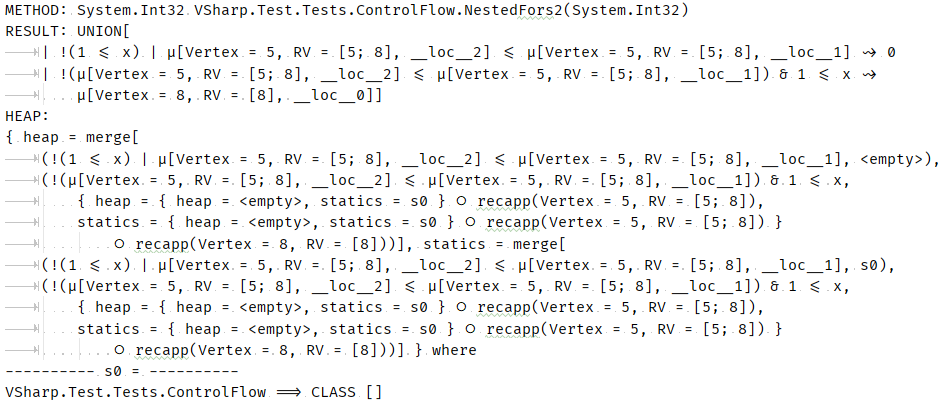
\includegraphics[scale=0.5]{Batoev/images/results.PNG}
\caption{Результат символьного исполнения метода~\ref{example:fors}}
\end{figure}

\begin{table}[t]
    \centering
    \begin{tabular}{ |p{3cm}||p{2cm}|p{2cm}|p{2cm}|  }
        \hline
        \multicolumn{4}{|c|}{Количественные характеристики тестов} \\
        \hline
        Название тестового набора &Количество тестов в наборе&Количество успешно пройденных тестов&Количество инструкций CIL\\
        \hline
        Arithmetics   &80    &77    &1968\\
        Logics        &75    &75    &1458\\
        Conditional   &10    &6     &943\\
        Recursive     &5     &5     &751\\
        Lambdas       &2     &2     &404\\
        Generic       &14    &14    &194\\
        Strings       &15    &15    &219\\
        Unsafe        &16    &16    &312\\
        Typecast      &19    &19    &969\\
        Methods       &10    &10    &238\\
        Lists         &9     &9     &1420\\
        Chess.NET     &1     &1     &2723\\
        \hline
        Всего         &256   &249   &11599\\
        \hline
    \end{tabular}
    \captionof{table}{Результаты тестирования}
    \label{experiments}
\end{table}


\FloatBarrier

\subsection{Тестирование интерпретатора}
Тестирование нового интерпретатора проводилось на тестовой подсистеме проекта <<VSharp.Test>> и на библиотеке \textsc{Chess.NET}.
Подсистема содержит тестовые наборы, затрагивающие различные конструкции и возможности языка C\#:
арифметику, логические операции,
работу с массивами разных размерностей, генерирование исключений, тесты на классы и структуры, включающие взаимодействие со статическими членами и вызовы виртуальных методов,
тесты с неограниченной рекурсией, тесты с \emph{unsafe}-кодом, тесты со строками. 

Таблица~\ref{experiments} показывает результаты проведенного тестирования. 
В наборах тестах с арифметикой и условными конструкциями была часть тестов с генерацией исключений. 
Поскольку схема обработки исключений для языка CIL не была реализована, то данные тесты были некорректно исполнены.
По той же причине не было проведено тестирования на тестовым наборе <<TryCatch>>, 
основное предназначение которого --- инициирование и перехват исключений.

\section{Заключение}

В данной работе описан подход к композициональному символьному исполнению без раскрутки. Была предложена концепция композициональной памяти с символьной адресацией. Был доказан некоторый набор свойств КСП, дающий основание для подхода в стиле систем переписывания, где символьные кучи могут сами выступать как символы. Это даёт возможность автоматически порождать уравнения на состояния, решения которых в точности отражают поведения функций, работающих с динамической памятью. Было показано как свести задачу решения уравнений на состояния к задаче проверки безопасности чистых функций второго порядка.

Данная работа нацелена на теоретические основания композиционального анализа динамической памяти. Мы оставляем апробацию этого подхода на будущее. Другим направлением будущих исследований может быть расширение нашего формализма на композициональный анализ параллельных программ.

\bibliographystyle{ugost2008ls}
\begin{thebibliography}{10}

\bibitem{baldoni2018survey}
Roberto Baldoni, Emilio Coppa, Daniele~Cono D’elia, Camil Demetrescu, and
  Irene Finocchi.
\newblock A survey of symbolic execution techniques.
\newblock {\em ACM Computing Surveys (CSUR)}, 51(3):50, 2018.

\bibitem{godefroid2007compositional}
Patrice Godefroid.
\newblock Compositional dynamic test generation.
\newblock In {\em ACM Sigplan Notices}, volume~42, pages 47--54. ACM, 2007.

\bibitem{jaffar2012tracer}
Joxan Jaffar, Vijayaraghavan Murali, Jorge~A Navas, and Andrew~E Santosa.
\newblock Tracer: A symbolic execution tool for verification.
\newblock In {\em International Conference on Computer Aided Verification},
  pages 758--766. Springer, 2012.

\bibitem{king1976symbolic}
James~C King.
\newblock Symbolic execution and program testing.
\newblock {\em Communications of the ACM}, 19(7):385--394, 1976.

\bibitem{kuznetsov2012efficient}
Volodymyr Kuznetsov, Johannes Kinder, Stefan Bucur, and George Candea.
\newblock Efficient state merging in symbolic execution.
\newblock {\em Acm Sigplan Notices}, 47(6):193--204, 2012.

\bibitem{mcmillan2010lazy}
Kenneth~L McMillan.
\newblock Lazy annotation for program testing and verification.
\newblock In {\em International Conference on Computer Aided Verification},
  pages 104--118. Springer, 2010.

\bibitem{kostyukov2018csewu}
Юрий~Олегович Костюков.
\newblock {\em Кучи как чистые функции:
  композициональное символьное исполнение
  без раскрутки}, pages 288--346.
\newblock 6. 2018.

\end{thebibliography}

\title{Композициональное символьное исполнение CIL-кода}

\titlerunning{Композициональное символьное исполнение CIL-кода}

\author{Батоев Константин Аланович}

\authorrunning{К.~А.~ Батоев}

\tocauthor{Константин Батоев}
\institute{St Petersburg State University\\
	\email{konstantin.batoev@gmail.com}}

\maketitle

% \renewcommand{\ttdefault}{cmtt}

\newsavebox\CBox
\newcommand\hcancel[2][0.1pt]{%
  \ifmmode\sbox\CBox{$#2$}\else\sbox\CBox{#2}\fi%
  \makebox[0pt][l]{\usebox\CBox}%
  \textcolor{red}{\rule[0.3\ht\CBox-#1/2]{\wd\CBox}{#1}}}

\captionsetup[figure]{name=Рисунок}

% \newtheorem*{proof}{Доказательство}

\renewcommand{\defnautorefname}{опр.}
\renewcommand{\lemautorefname}{лемм.}
\renewcommand{\remkautorefname}{зам.}
\renewcommand{\propautorefname}{св.}
\renewcommand{\exmpautorefname}{пр.}
\renewcommand{\thmautorefname}{теор.}
% \renewcommand{\crlrautorefname}{Corollary}
\renewcommand{\sectionautorefname}{разд.}
\newcommand{\algorithmautorefname}{лист.}
\newcommand{\algorithmcfname}{Листинг}
\makeatletter
\renewcommand{\ALG@name}{Листинг}
\makeatother

\algrenewcommand\alglinenumber[1]{\tiny #1:}

\lstdefinelanguage{Demo}
{
 morecomment = [l]{//}, 
 sensitive = true,
 morekeywords = {type, new, null,
   bool, int, write, read,
   fail, nop, let, alloc, in,
   if, then, else, call,
   true, false, and, or, not}
}

\definecolor{commentgreen}{RGB}{0,200,100}
\lstdefinestyle{demolang}{language=Demo,
    rulecolor=\color{blue!80!black},
    basicstyle=\ttfamily\footnotesize,
    keywordstyle=\color{blue}\ttfamily,
    stringstyle=\color{red}\ttfamily,
    commentstyle=\color{commentgreen}\ttfamily,
    numbers=left,
    numbersep=5pt,
    numberstyle=\tiny\color{black},
    escapechar=@,
    tabsize=2
}

\usemintedstyle{vs}

\counterwithin{lstlisting}{section}
\counterwithin{algocf}{section}

\fontfamily{times}
% \fontsize{10pt}{30pt}
\selectfont
\setlength{\parindent}{0em}
% \setlength{\parskip}{1em}
\renewcommand{\baselinestretch}{1.0}

\SetupFloatingEnvironment{listing}{name=Листинг}
\providecommand*{\listingautorefname}{лист.}
\renewcommand*{\figureautorefname}{рис.}
\renewcommand*{\tableautorefname}{табл.}
\SetAlgorithmName{Листинг}{лист.} 

\theoremstyle{plain}
\newtheorem{thm}{Теорема}%[section]
\newtheorem{lem}{Лемма}%[section]
% \newtheorem{crlr}{Corollary}%[section]

\theoremstyle{definition}
\newtheorem{defn}{Определение}
\newtheorem{remk}{Замечание}
\newtheorem*{remk*}{Замечание}
\newtheorem{prop}{Утверждение}
\newtheorem{exmp}{Пример}
% \newtheorem*{proof}{Доказательство}

% \newcommand{\defnautorefname}{опр.}
\newcommand{\lemautorefname}{лем.}
\newcommand{\remkautorefname}{зам.}
\newcommand{\propautorefname}{утв.}
\newcommand{\exmpautorefname}{пример}
\newcommand{\thmautorefname}{теор.}
% \renewcommand{\crlrautorefname}{Corollary}
\renewcommand{\sectionautorefname}{секция}
% \renewcommand{\algorithmautorefname}{Алгоритм}
% \renewcommand{\algorithmcfname}{Алгоритм}

% \renewcommand*{\Authsep}{\authorcr}
% \renewcommand*{\Authand}{\authorcr}
% \renewcommand*{\Authands}{\authorcr}

% \makeatletter
% \makeatother

\lstdefinelanguage{Demo}
{
 morecomment = [l]{//}, 
 sensitive = true,
 morekeywords = {new, null,
   fail, goto, halt,
   true, false, and, or, not}
}

\definecolor{commentgreen}{RGB}{0,200,100}
\lstdefinestyle{demolang}{language=Demo,
    rulecolor=\color{blue!80!black},
    basicstyle=\ttfamily\footnotesize,
    keywordstyle=\color{blue}\ttfamily,
    stringstyle=\color{red}\ttfamily,
    commentstyle=\color{commentgreen}\ttfamily,
    numbers=left,
    numbersep=5pt,
    numberstyle=\tiny\color{black},
    escapechar=@,
    tabsize=2
}

%%% For graph drawing
\definecolor {processblue}{cmyk}{0.96,0,0,0}
\definecolor {processgreen}{cmyk}{1,0,1,0}
\definecolor {processred}{cmyk}{0, 0.84, 0.80, 0.19}
\definecolor {processyellow}{cmyk}{0, 0, 1, 0}


%\newcommand{\csharp}[1]{\mintinline{csharp}{#1}}

\newcommand{\pex}{\textsc{Pex}}
\newcommand{\predator}{\textsc{Predator}}
\newcommand{\dotnet}{\textsc{.NET}}
\newcommand{\clang}{\textsc{C}}
\newcommand{\vsharp}{\textsc{V\#}}

\newcommand\addrset{loc}
\newcommand\termset{term}
\newcommand\guardset{guard}

\newcommand\eqby[1]{\mathrel{\stackrel{\mbox{\normalfont\tiny #1}}{=}}}
\newcommand\eqdef{\eqby{def}}

\newcommand\aite{ite}
\newcommand\ite[3]{\aite(#1,#2,#3)}
\newcommand\Ite[3]{\aite\big(#1,#2,#3\big)}
\newcommand\pair[2]{\langle#1, #2\rangle}
\newcommand\paiR[2]{\big\langle#1, #2\big\rangle}
\newcommand\mg[2]{#1=#2}
\newcommand\nmg[2]{#1\neq#2}
\newcommand\li[1]{LI(#1)}
\let\emptyheap\varepsilon
\newcommand\agrec{Rec}
\newcommand\agmerge{Merge}
\newcommand\agcompose{\bigcirc}
\newcommand\GRec[1]{\agrec\big(#1\big)}
\newcommand\GMerge[1]{\agmerge\big(#1\big)}
\newcommand\GCompose[2]{#1\agcompose#2}
\newcommand\agho{App}
\newcommand\gapp[1]{\agho(#1)}
\newcommand\GApp[1]{\agho\big(#1\big)}
\newcommand\aunion{\texttt{UNION}}
\newcommand\union[1]{\aunion\big(#1\big)}
\newcommand\Union[1]{\aunion\Big(#1\Big)}
\newcommand\aderef{readStore}
\newcommand\readTerm{readTerm}
\newcommand\writeTerm{writeTerm}
\newcommand\afind{find}
\newcommand\find[5]{\afind(#1,#2,#3,#4,#5)}
\newcommand\finD[5]{\afind\big(#1,#2,#3,#4,#5\big)}
\newcommand\Find[5]{\afind\Big(#1,#2,#3,#4,#5\Big)}
\newcommand\deref[2]{\aderef(#1,#2)}
\newcommand\Deref[2]{\aderef\big(#1,#2\big)}
\newcommand\compose[2]{#1\circ#2}
\newcommand\lmbd[2]{\lambda #1.#2}
\newcommand\lmbdx[1]{\lambda x.#1}
\newcommand\dom[1]{dom(#1)}
\newcommand\Dom[1]{dom\big(#1\big)}

\newcommand\Li[1]{LI\big(#1\big)}
\newcommand\amutate{writeStore}
\newcommand\amutateStack{writeStack}
\newcommand\mutate[3]{\amutate(#1,#2,#3)}
\newcommand\mutateStack[4]{\amutateStack(#1,#2,#3,#4)}
\newcommand\rdbodyext[6]{\Union{\big\{\paiR{#4\mg{#1}{#5}}{#6\big(#2(#5), xs\big)} \mid #5\in\dom{#2} \big\}\\&\qquad\qquad\qquad\cup\paiR{#4\bigwedge_{\mathclap{#5\in\dom{#2}}}{\nmg{#1}{#5}}}{#6\big(#3, xs\big)}}}
\newcommand\rdbody[4]{\rdbodyext{#1}{#2}{#3}{}{l}{#4}}
\newcommand\wrtbody[6]{\Union{&\paiR{\mg{#1}{#2}}{\writeTerm\big(#3,#4,#6\big)},
    \\&\paiR{\nmg{#1}{#2}}{\writeTerm\big(#5(#1),#4,#6\big)}}}
\newcommand{\var}[1]{\mathit{#1}}


\begin{abstract}
Известно, что наибольшую сложность в области верификации программ представляет задача доказательства корректности программ с циклическими участками кода. Опираясь на подход символьного исполнения программ и на введенные формализмы обобщённых куч в работе~\cite{kostyukov2018csewu}, данная работа представляет алгоритм композиционального символьного исполнения без раскрутки отношения перехода программ с произвольным графом потока управления. На его основе был реализован символьный интерпретатор языка CIL в проекте V\#, символьной виртуальной машине для анализа .NET. Была проведена апробация алгоритма на примерах, включающих сложные потоки управления, и интерпретатора на тестовой базе проекта VSharp.Test и на библиотеке Chess.NET.
\end{abstract}
\section*{Введение}
Поиск путей в графе с ограничением в виде формальных языков~\cite{FLCpathProblem} --- это задача, в которой формальные языки используются для задания множества искомых путей. В таком подходе каждый путь соответствует слову, состоящему из меток его рёбер, а ограничением на путь является принадлежность соответствующего ему слова некоторому заданному формальному языку.

В качестве класса формальных языков по иерархии Хомского наибольший интерес представляют контекстно-свободные языки. В отличие от регулярных они обладают большей выразительностью. Поэтому в задаче поиска путей контекстно-свободные ограничения позволяют задавать более сложные отношения между вершинами. Так, например, важный класс запросов поиска вершин, лежащих на одном уровне иерархии~\cite{zhlang-2016}, задаётся только контекстно-свободными, но не регулярными ограничениями. Запросы такого вида, как и другие запросы с контекстно-свободными ограничениями имеют широкое применение в биоинформатике~\cite{bio-application} и при обработке rdf-файлов~\cite{zhlang-2016}.

Наиболее удобным и подходящим инструментом для работы с граф\-структурированными данными являются графовые базы данных. Так же как и реляционные, графовые базы данных поддерживают свой язык запросов. С его помощью графовые базы данных позволяют решать вышеупомянутую задачу поиска путей. Но ограничения на пути, которые поддерживается в наиболее распространённых базах данных, являются в лучшем случае регулярными.

Отсутствие поддержки контекстно-свободных ограничений в графовых базах данных, во-первых, сильно ограничивает выразительность языка запросов. Во-вторых, при необходимости в более сложных запросах разработчикам приходится самим писать алгоритмы, решающие задачу контекстно-свободной достижимости для их частного случая. Так, например, Хуэй Мяо и др.~\cite{datascince-lifecycle} разработали систему хранения и отслеживания версий артефактов, возникающих при научных работах. Вся информация про артефакты хранилась в графовой базе данных. При этом при разработке возникла потребность в выполнении запросов с контекстно-свободными ограничениями для выявления взаимоотношений между различными версиями различных артефактов. Это и послужило началом статьи~\cite{datascince-lifecycle}, в которой приводятся алгоритмы решения частных запросов.

В недавнем исследовании Йохем Куйперс и др.~\cite{Kuijpers:2019:ESC:3335783.3335791} произвели сравнительный анализ наиболее известных алгоритмов поиска путей с конте\-кстно-свободными ограничениями. Алгоритмы запускались на графах, находящихся в хранилище графовой базы данных Neo4j. По результатам исследования было показано, что в контексте Neo4j алгоритмы обладают большим временем работы, и поэтому дальнейшая работа по расширению языка запросов прекратилась. При этом Рустам Азимов~\cite{Azimov:2018:CPQ:3210259.3210264} предоставил матричный алгоритм и его реализацию, которая работает за разумное время на реальных данных. Но, так как алгоритм был реализован вне контекста базы данных, его результат приняли недостаточно показательным. Поэтому вопрос о реализуемости запросов с контекстно-свободными ограничениями в графовых базах данных, а соответственно и о возможности расширения языка запросов для их поддержки остаётся открытым.

\section{Постановка задачи}
Целью данной работы является полная поддержка запросов с конте\-кстно-свободными ограничениями для графовой базы данных. А именно, необходимо предоставить пользователю возможность формулировать запросы с контекстно-свободными ограничениями в терминах одного из существующих стандартных языков запросов и исполнять их в графовой базе данных за приемлемое время. Для достижения этой цели были поставлены следующие задачи.

\begin{itemize}
    \item Выполнить обзор существующих реализаций поддержки запросов с контекстно-свободными ограничениями в графовых базах данных. В результате обзора необходимо выбрать наиболее перспективный с точки зрения производительности алгоритм решения задачи контекстно-свободной достижимости и подходящую для его интеграции базу данных. При выборе базы данных необходимо учитывать как возможность интеграции выбранного алгоритма, так и возможность поддержки одного из стандартных языков запросов, позволяющего выражать контекстно-свободные ограничения.
    \item Интегрировать выбранный на предыдущем шаге алгоритм в выбранную графовую базу данных.
    \item Расширить язык запросов выбранной базы данных конструкциями, необходимыми для выражения контекстно-свободных ограничений.
    \item Произвести замеры производительности полученного решения и сравнить его с существующими решениями.
\end{itemize}


\section{Обзор}

\subsection{Терминология}
Контекстно-свободной грамматикой называется $G = (\Sigma, N, P, S)$, где $\Sigma$ --- алфавит терминальных символов, $N$ --- алфавит нетерминальных символов, $P$ --- множество правил вида $A \rightarrow \alpha$, где $A \in N$, $\alpha \in (\Sigma \cup N)^*$, а $S \in N$ --- выделенный стартовый нетерминал.

% \gsv{про S забыли}.

Языком $L$ над алфавитом $\Sigma$ называется любое подмножество $2^{\Sigma^*}$. Языком, порождаемой грамматикой G, является множество $L(G) = \{S \xRightarrow{*} \beta, \beta \in \Sigma^*\}$, где $S \xRightarrow{*} \beta$ означает, что из нетереминала $S$ путём последовательного применения правил грамматики выводится $\beta$.

Контекстно-свободная грамматика $G = (\Sigma, N, P, S)$ находится в осла\-бленной нормальной форме Хомского, если любое её правило имеет вид $A \rightarrow BC$, где $A, B, C \in N$, либо $A \rightarrow a$, где $A \in N, a \in \Sigma$. В отличие от нормальной формы Хомского в ослабленной, во-первых, допускается присутствие стартового нетерминала $S$ в правых частях правил грамматики, во-вторых, запрещаются правила вида $S \rightarrow \epsilon$, где $\epsilon$ --- пустая строка.

% \gsv{Это не нормальная форма Хомского. У НФХ есть дополнительные ограничения. Мы называем то, что здесь, ослабленной НФХ. Важно отдельно проговорить разницу с НФХ.}

В задаче поиска путей с ограничениями в виде формальных языков дан граф $(V, E)$, разметка его рёбер $l: E \rightarrow \Sigma$ и язык $L$ над алфавитом $\Sigma$. Требуется найти множество всех пар вершин, между которыми существует путь, метки на рёбрах которого образуют слово в заданном языке. То есть требуется найти следующее множество:
\[\{(v, to): \exists p=(e_1,...,e_n) \in E^*: l(e_1)...l(e_n) \in L,~src(e_1)=v,~dst(e_n)=to\}\]
Здесь $src(e)$ и $dst(e)$ для $e \in E$ означают начальную и конечную вершину ребра $e$. В данном контексте язык $L$ называется языком ограничений.
% \gsv{У Вас вершины v и to никак с путём не связаны}

Задача поиска путей с контекстно-свободными ограничениями --- это задача поиска путей в виде формальных языков, в которой язык задаётся контекстно-свободной грамматикой.

\subsection{Графовые базы данных}
Графовые СУБД\footnote{СУБД --- Система управления базами данных} (далее просто графовые базы данных) --- это разновидность СУБД, в которой данные хранятся в виде графов. В отличие от других разновидностей, в графовых базах данных отношения между объектами так же важны, как и сами объекты.

Основной моделью представления графов в таких базах данных является gpraph property model~\cite{graph-propery-model}. В ней каждая сущность может содержать набор свойств в формате ключ-значение. Основными сущностями являются узлы и отношения. Узлы соответствуют вершинам графа и помимо свойств могут иметь несколько меток. Отношения соответствуют рёбрам и имеют ровно одну метку, которая называется типом отношения. На рисунке~\ref{fig:graph_bd_1} показан небольшой пример графа в такой модели. 

\begin{figure}[h]
\centering
    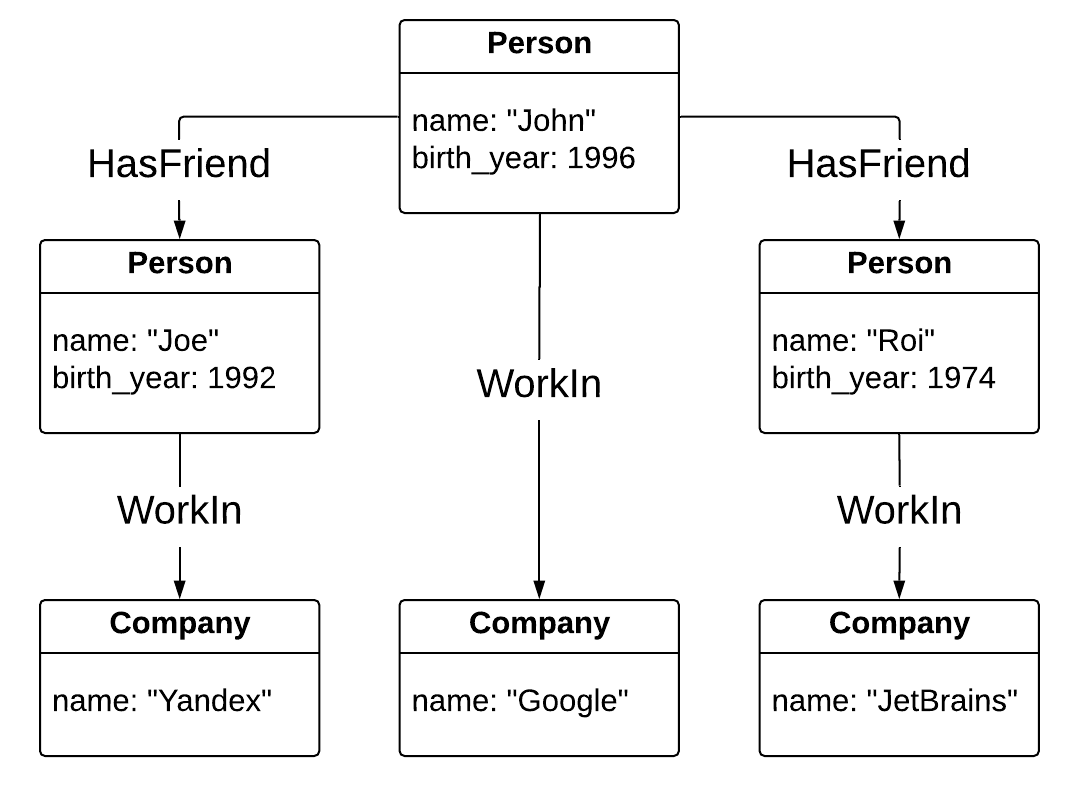
\includegraphics[width=0.7\linewidth]{Terekhov/pictures/graph_bd_1.png}
    \caption{Пример социального графа}
    \label{fig:graph_bd_1}
\end{figure}

Для работы с графами графовые базы данных предоставляют язык запросов, самым популярным из которых является Cypher~\cite{cypher-language}. В нём главный интерес представляют запросы вида сопоставления с образцом. Они позволяют задавать интересующие пути или подграфы в виде шаблонов и описывать информацию, которую нужно извлечь после удачного сопоставления. На рисунке~\ref{code:cypher_query} приведён пример такого запроса. Шаблон пути описывается в выражении MATCH. В нём между круглыми скобками задаются шаблоны вершин, а между квадратными шаблоны рёбер. Таким образом в данном примере задаются следующие ограничения: путь должен начинаться из вершины с меткой Person и именем John и состоять из двух рёбер, первое из которых должно иметь тип HasFriend, а второе WorkIn. В выражении RETURN задаётся информация, которую нужно извлечь. В данном примере это имя последней в пути вершины. В итоге ответом на такой запрос являются имена компаний, в которых работают друзья Джона. Результатом работы этого запроса на графе из рисунка~\ref{fig:graph_bd_1} является множество \{"Yandex", "JetBrains"\}.

%\lstset{
%   basicstyle=\fontsize{14}{14}\selectfont\ttfamily
%}

\begin{figure}[h]
\begin{lstlisting}[language=sql]
MATCH (p:Person)-[:HasFriend]->()-[:WorkIn]->(to)
WHERE p.name = "John"
RETURN to.name
\end{lstlisting}
\caption{Пример конечного запроса на языке Cypher}
\label{code:cypher_query}
\end{figure}

С формальной точки зрения шаблоны пути в выражении MATCH позволяют поставить задачу поиска путей с ограничениями в виде формальных языков. Так в запросе на рисунке~\ref{code:cypher_query} языком ограничений является конечный язык $\{(HasFriend, WorkIn)\}$. Для запроса на рисунке~\ref{code:cypher_query_2} ограничением является регулярный язык $\{A, B\}^*$. 

\begin{figure}[h]
\begin{lstlisting}[language=sql]
MATCH (v)-[:A | :B *]->(to)
RETURN to.name
\end{lstlisting}
\caption{Пример регулярного запроса на языке Cypher}
\label{code:cypher_query_2}
\end{figure}

При этом регулярные ограничения поддерживаются лишь частично и позволяют искать только пути произвольной длины с заданными метками на рёбрах, а более глубокие регулярные выражения не поддерживаются. Поэтому на текущий момент язык запросов довольно ограничен.

\subsection{Существующие решения}
Как было упомянуто раннее, ни одна графовая база данных не поддерживает запросов с контекстно-свободными ограничениями. Тем не менее существуют альтернативные решения поддержки таких запросов. 

\subsubsection{Парсер-комбинаторы для Neo4j}\label{sec:pareser-combinators}
В 2018 году группой исследователей из JetBrains Research на основе библиотеки Meerkat была разработана библиотека для поддержки запросов с контекстно-свободными ограничениями~\cite{parser-combinators}. Она использует графовую базу данных Neo4j~\cite{neo4j} как хранилище графов и позволяет задавать запросы в виде парсер-комбинаторов. Основным достоинством данной работы является то, что с помощью этой библиотеки кроме контекстно-свободных запросов можно выразить базовую часть языка Cypher. Но так как конкурировать с оригинальной реализацией выполнения запросов Neo4j очень сложно, это достигается вместе c сильной потерей производительности. Кроме этого контекстно-свободные запросы обрабатываются также достаточно медленно.

Таким образом данное решение является альтернативой языка запросов Neo4j, а не его расширением. Из-за медленного времени работы такое решение подходит только для работы с небольшими графами. 

\subsubsection{Расширение языка запросов SPARQL}\label{subsection:cypher-extention-2}
%Про sparql%
В 2016 Сяованг Чжан предоставил язык cfSPARQL~\cite{zhlang-2016} --- расширение языка SPARQL, который способен выразить запросы с контекстно-свободными ограничениями. Также он привёл алгоритм для вычисления таких запросов и замеры производительности. Но, во-первых, работа была сделана вне контекста графовой базы данных, а во-вторых, время работы предложенного алгоритма было больше, чем время работы парсер-комбинаторов.

\subsubsection{Существующие реализации алгоритмов решения задачи контекстно-свободной достижимости}
Основной сложностью расширения языка запросов для поддержки запросов с контекстно-свободными ограничениями является долгое время работы соответствующих алгоритмов. Так, например, в 2019 году Йохем Куйперс и другие исследователи с целью попытки расширения языка запросов Cypher для графовой базы данных Neo4j произвели сравнительный анализ производительности наиболее известных алгоритмов решения задачи контекстно-свободной достижимости.

В данном исследовании были рассмотрены и произведены замеры времени работы алгоритма Элле Хелингса~\cite{hellings-2015}, основанного на атрибутных грамматиках, восходящего алгоритма Фреда Сантоса~\cite{santos-2018}, матричного алгоритма Рустама Азимова~\cite{Azimov:2018:CPQ:3210259.3210264} и алгоритма Петтери Севона~\cite{bio-application}. Все алгоритмы были интегрированы в Neo4j и запускались на графах, находящихся в её хранилище. Алгоритмы были написаны на языке Java, при этом их реализация являлась однопоточной.

% \gsv{В таких местах надо сразу ссылку на алгоритм давать.}

По результатам замеров производительности было показано, что время работы алгоритмов является слишком большим и неприемлемым для широкого практического использования. Поэтому дальнейшая работа по интеграции и расширению языка запросов была приостановлена.

Тем не менее, матричный алгоритм Рустама Азимова в сравнительном анализе Йохема Куйперса был реализован без необходимых матричных библиотек, которые могут сильно уменьшить время его работы. Так, например, в исследовании Никиты Мишина и др.~\cite{azimov-evalution} был произведён сравнительный анализ времени работы нескольких реализаций алгоритма Рустама Азимова, основанных на различных специализированных матричных библиотеках. Графы и запросы к ним были взяты из объемлющего набора данных CFPQ\_Data~\cite{cfpq-data}, предоставленного лабораторией языковых инструментов JetBrains Research. 

Результаты замеров Никиты Мишина и др. показали, что при грамотной реализации алгоритма Рустама Азимова и использовании подходящих матричных библиотек можно добиться очень высокой производительности. Поэтому, так как основной проблемой применимости запросов с контекстно-свободными ограничениями является долгое время работы соответствующих алгоритмов, в качестве алгоритма решения задачи конте\-кстно-свободной достижимости был выбран матричный алгоритм Рустама Азимова.

\subsection{Матричный алгоритм Рустама Азимова}\label{sec:matrix-algo}
Выбранный в предыдущей главе алгоритм Рустама Азимова~\cite{Azimov:2018:CPQ:3210259.3210264}, в отличие от других алгоритмов решения задачи контекстно-свободной достижимости~\cite{hellings-2015, santos-2018, zhlang-2016}, работает с графами в виде разреженных матриц смежности. Данный алгоритм состоит из последовательности операций над разреженными матрицами, время работы которых зависит не от размеров матричных операндов, а от количества их ненулевых элементов.

На вход алгоритму (см. алгоритм 1) поступает помеченный граф $D=(V,E)$ и контекстно-свободная грамматика $G=(\Sigma, N, P, S)$ в ослабленной нормальной форме Хомского. Для каждого нетерминала $A$ в ассоциативном массиве $T$ хранится соответствующая ему булева матрица $T[A]$. На всём этапе алгоритма поддерживается следующий инвариант: $T[A]_{i,j} = 1$ равносильно существует пути, метки на рёбрах которого образуют слово, выводящееся из нетерминала $A$. На первом этапе происходит инициализация матриц с помощью простых правил грамматики, после чего инвариант выполняется для всех путей единичной длины. На втором этапе происходит транзитивное замыкание, после чего этот инвариант верен для всех путей. Результатом данного алгоритма является матрица, соответствующая стартовому нетерминалу $S$.

%  Это позволяет для его реализации использовать многопоточные матричные библиотеки, с помощью которых можно добиться очень высокой производительности. Поэтому на текущий момент алгоритм Рустама Азимова показывает наилучшее время работы на практике.

\begin{algorithm}
\caption{Матричный алгоритм Рустама Азимова}

\begin{algorithmic}[1]
\Function{contextFreePathQuerying}{$D$, $G$}
    \State{$n =$ getNodeCount(D)}
    \State{$N =$ getAllNonterms(G)}
    \State{$E =$ getEdges($D$)}
    \State{$P =$ getRules($G$)}
    \State{$S =$ getStartNonterm($G$)}
    \State{$T = \{A \rightarrow \varnothing_{n \times n} : A \in$ $N$ \} }
    \ForAll{$(v, to, label) \in E$}
    \Comment{Инициализация матриц}
        \ForAll{$A \rightarrow label \in P$}
            \State{$T[A]_{i,j} = 1$}
        \EndFor
    \EndFor    
    \While{$\exists A: T[A]$ is changing}
    \Comment{Вычисление замыкания}
        \ForAll{$A \rightarrow BC \in P$}
            \State{$T[A] \oplus= T[B] \otimes T[C]$}
        \EndFor
    \EndWhile
\State \Return $T[S]$
\EndFunction

\end{algorithmic}
\end{algorithm}

Практическое время работы алгоритма Рустама Азимова сильно зависит от производительности используемой матричной библиотеки. Это накладывает некоторые ограничения на выбор подходящей графовой базы данных, так же как и возможность представления графов в матричном виде.

\subsection{RedisGraph}
RedisGraph~\cite{redis-graph} --- это высокопроизводительная графовая база данных, поддерживающая язык запросов Cypher. В отличие от наиболее распространённой графовой базы данных Neo4j~\cite{neo4j}, RedisGraph написан на языке Си и для работы с данными использует Redis~\cite{redis}, основным достоинством которого является возможность хранить данные прямо в оперативной памяти. Это позволяет RedisGraph быстро обрабатывать пользовательские запросы.

Также RedisGraph является единственной графовой базой данных, которая работает с графами в виде разреженных матриц смежности и транслирует запросы языка Cypher в матричные выражения. Для представления графов в таком виде и работы с ними в терминах линейной алгебры используется мощный матричный фреймворк GraphBlas~\cite{graph-blas}. Его реализация SuiteSparse~\cite{suite-sparse} является многопоточной и сильно оптимизирована, что позволяет RedisGraph добиться высокой производительности.

Из всего этого следует, что RedisGraph идеально подходит для интеграции матричного алгоритма. Во-первых, графы представляются в необходимом алгоритму виде, что позволит избежать издержек на конвертацию форматов. Во-вторых, использование SuiteSparse для вычисления матричных операций позволит добиться высокой производительности. Поэтому RedisGraph был выбран в качестве графовой базы данных для интеграции матричного алгоритма и расширения языка запросов.

% Так как алгоритм Рустама Азимова работает с матричным представлением графа,, как наиболее подходящий для интеграции матричного алгоритма.

\subsection{Расширение языка Cypher}\label{subsection:cypher-extention}
На текущий момент оригинальная версия языка Cypher, используемая в том числе и в RedisGraph, не поддерживает запросов с контекстно-свободными ограничениями. Но тем не менее в 2017 году был разработан черновой вариант спецификации расширения Cypher~\cite{cypher-specification}, которая вводит в язык шаблоны путей. Они позволяют выразить более сложные запросы, в том числе запросы с контекстно-свободными ограничениями.

Шаблоны путей являются альтернативой шаблонам рёбер, которые есть в оригинальном Cypher. Они, как и шаблоны рёбер, могут встречаться в выражении MATCH и иметь своё направление. Кроме этого в глобальной области запроса им можно задавать имя, на которое потом можно ссылаться внутри других шаблонов.

Шаблон пути представляет из себя регулярное выражение над некоторыми примитивами. В качестве таких примитивов могут выступать шаблоны рёбер, шаблоны вершин и ссылки на именованные шаблоны путей. Также любым подвыражениям можно задавать своё направление. Основная часть конкретного синтаксиса данного расширения приведена на рисунке~\ref{fig:cypher_syntax}.

\begin{figure}[]
\begin{align*}
\begin{split}
PathPattern     &= ["<"],~"-/",~PathExpression,~"/-",~[">"]\\
PathExpression  &= \{PathAlternative\}\\
PathAlternative &= PathRepetition,~\{"|", PathRepetition\}\\
PathRepetition  &= ["<"],~PathBase,~[">"],~("*")
\end{split}\\
\begin{split}
PathBase &= PathEdge \\
         &~~|~PathNode \\
         &~~|~PathReference \\
         &~~|~"[",~PathExpression,~"]"
\end{split}\\
\begin{split}
PathEdge      &= Label \\
PathNode      &= "(",~[Label,~\{"|",~Label\}],~")" \\
PathReference &= "\sim",~SymbolicName; \\
Label         &= ":",~LabelName
\end{split}
\end{align*}
\caption{Расширение конкретного синтаксиса Cypher}
\label{fig:cypher_syntax}
\end{figure}

Каждый шаблон пути задаёт отношение на множестве вершин. Поэтому семантикой языка шаблонов путей $L_{P}$ в контексте графа $G(V, E)$ является отображение $\llbracket \cdot \rrbracket_{G}: L_P \rightarrow V \times V$, которое каждому шаблону $p\in L_P$ сопоставляет множество пар вершин, между которыми существует путь, удовлетворяющий данному шаблону $p$. 

Подробное описание данной семантики приводится в таблице~\ref{tab:cypher_sematic}.  В ней наибольший интерес представляют именованные шаблоны путей, так как именно с помощью них можно выразить запросы с контекстно-свободными ограничениями. Все именованные шаблоны путей $S_i = p_j$ можно рассматривать как правила контекстно свободной грамматики с алфавитом нетерминалов $\{S_i\}_{i=1}^n$. Тогда каждый нетерминал $S_j$ порождает язык $L_{S_j} \subset L_p$, а семантикой соответствующего именованного шаблона пути $S_j=p_j$ является множество $\bigcup\limits_{p \in L_{s_j}} \llbracket p \rrbracket_{G}$.

На рисунке~\ref{code:cypher_query_3} приведён пример запроса в расширенном синтаксисе. В нём декларируется именованный шаблон S, который задаёт множество правильных скобочных последовательностей над ребрами с типом L и R. Далее в выражении MATCH задаётся шаблон пути, состоящий из ссылки на шаблон S. Таким образом результатом обработки запроса является множество всех пар вершин, между которыми существует путь, метки на рёбрах которого образуют правильную скобочную последовательность. 

\begin{table}[h!]
\begin{adjustbox}{max width=\textwidth}
\begin{tabular}{|c|c|c|}
\hline
$p \in L_P$                                                                                  & $\llbracket p \rrbracket_{G}$                                                                                                                                                                                   & Описание шаблона пути                                                                                                         \\ \hline
\hline
()                                                                                            & $\{(v, v): v \in V\}$                                                                                                                                                                                           & \begin{tabular}[c]{@{}c@{}}Пустой путь, состоящий из \\ одной произвольной вершины\end{tabular}                               \\ \hline
:a                                                                                            & $\{e=(v,to): e \in E, type(e)=a\}$                                                                                                                                                                              & \begin{tabular}[c]{@{}c@{}}Путь единичной длины,\\  состоящий из ребра с типом $a$\end{tabular}                               \\ \hline
(:b)                                                                                          & $\{(v, v): v \in V, label(v)=b\}$                                                                                                                                                                               & \begin{tabular}[c]{@{}c@{}}Пустой путь, состоящий из одной\\  вершины, помеченной меткой $b$\end{tabular}                     \\ \hline
$\alpha~\beta$                                                                                & $\llbracket \alpha \rrbracket_{G}\circ \llbracket \beta \rrbracket_{G}$                                                                                                                                         & Конкатенация путей $\alpha$ и $\beta$                                                                                         \\ \hline
$\alpha~|~\beta$                                                                              & $\llbracket \alpha \rrbracket_{G}\cup \llbracket \beta \rrbracket_{G}$                                                                                                                                          & Альтренатива между путями $\alpha$ и $\beta$                                                                                  \\ \hline
$[\alpha]$                                                                                    & $\llbracket \alpha \rrbracket_{G}$                                                                                                                                                                              & \begin{tabular}[c]{@{}c@{}}Квадратные скобки позволяют \\ группировать  выражения \\ для задания ассоциативности\end{tabular} \\ \hline
\textless{}$\alpha$                                                                           & $\{(to, v): (v, to) \in \llbracket \alpha \rrbracket_{G}\}$                                                                                                                                                     & Путь, обратный к пути $\alpha$                                                                                                \\ \hline
\textless{}$\alpha$\textgreater{}                                                             & $\llbracket \alpha~|~$\textless{}$\alpha \rrbracket_{G} $                                                                                                                                                       & \begin{tabular}[c]{@{}c@{}}Альтернатива между путём $\alpha$ и\\ обратным к нему\end{tabular}                                 \\ \hline
$\alpha^*$                                                                                    & $\llbracket \alpha \rrbracket_{G}^{*}$                                                                                                                                                                          & \begin{tabular}[c]{@{}c@{}}Путь, состоящий из\\ конкатенации 0 или более путей $\alpha$\end{tabular}                          \\ \hline
\begin{tabular}[c]{@{}c@{}}$\{S_i = p_i\}_{i=1}^{n}$\\ -- named\\  path patterns\end{tabular} & \begin{tabular}[c]{@{}c@{}}$P = \{S_i \rightarrow p_i\}_{i=1}^n$\\ $Gram_j = (\Sigma, \{S_i\}_{i=1}^n, P, S_j)$\\ $\llbracket S_j \rrbracket_{G} = \bigcup\limits_{p \in L(G)}{\llbracket p \rrbracket_{G}}$\end{tabular} & Именнованые шалоны путей                                                                                                      \\ \hline
$\sim$$S$                                                                                     & $\llbracket S \rrbracket_{G}$                                                                                                                                                                                   & \begin{tabular}[c]{@{}c@{}}Ссылка на именнованный\\  шаблон пути\end{tabular}                                                 \\ \hline
\end{tabular}
\end{adjustbox}
\caption{Семантика языка шаблонов путей}
\label{tab:cypher_sematic}
\end{table}

\begin{figure}[h!]
\begin{lstlisting}[language=sql]
PATH PATTERN S = ()-/ [:L ~S :R] | [~S ~S] | () /-()
MATCH (v)-/ ~S /-(to)
RETURN v, to
\end{lstlisting}
\caption{Пример запроса в расширенном синтаксисе Cypher}
\label{code:cypher_query_3}
\end{figure}

Данная спецификация расширения Cypher была представлена официальными разработчиками и сильно расширяет выразительность языка, предоставляя удобную возможность выражать запросы как с регулярными, так и с контекстно-свободными ограничениями. Поэтому в моей работе приводится поддержка выполнения запросов именно для этого расширения языка.

% \gsv{Не хватает какого-то чёткого вывода про то, что вот именно это мы и буем использовать.}

\section{Реализация}
По результатам обзора было решено реализовать поддержку расширения языка Cypher, представленную в главе~\ref{subsection:cypher-extention}, для графовой базы данных RedisGraph. За основу алгоритма, решающего задачу поиска путей с контекстно-свободными ограничениями, был взят матричный алгоритм Рустама Азимова, описанный в главе~\ref{sec:matrix-algo}.

% \gsv{И зжесь надо ещё раз подитожить в духе "по результатм обзора было решено сделать то и это с использованием того и сего"}

\subsection{План выполнения запроса}\label{execution-plan}
В RedisGraph основной частью обработки запроса является построение плана его выполнения. Её часть, которая относится к шаблонам путей приведена на рисунке~\ref{fig:execution_plan}. В ней зелёным цветом выделено то, что было добавлено или расширено.

В самом начале, после получения запроса строится его абстрактное синтаксическое дерево \textit{AST}. Далее, из него извлекаются именованные и неименованные шаблоны путей \textit{PathPattern} и \textit{NamedPathPatterns}, после чего они преобразуются в более удобное промежуточное представление \textit{PathExpr}. При этом, для дальнейшего связывания ссылок, именованные шаблоны сохраняются в глобальном контексте запроса \textit{PathPatternCtx}.

На следующем этапе происходит трансляция промежуточных представлений \textit{PathExpr} в матричные выражения \textit{AlgebraicExpression}. В них операндами являются либо матрицы, полученные из указанного в запросе графа \textit{GraphCtx}, либо ссылки на именованные шаблоны путей из \textit{PathPatternCtx}. Основной идеей трансляции является то, что после вычисления матричного выражения получается матрица, которая задаёт то же самое отношение на множестве вершин, что и исходный шаблон пути.

Далее каждое такое выражение формирует новую операцию плана выполнения запроса \textit{CfpqTraverseOp}. При её вычислении сначала происходит запуск расширенной версии матричного алгоритма Рустама Азимова. Он решает задачу контекстно-свободной достижимости, заданной именованными шаблонами путей. После этого все ссылки в матричном выражении заменяются на полученные в ходе алгоритма матрицы и происходит вычисление матричного выражения. Каждая такая операция добавляется в план выполнения запроса.

%  \gsv{Используйте \textit{CfpqTraverseOp} вместо долларов для длинных слов. Они тогда не распадаются из-а лишних пробелов.}

\begin{figure}[H]
\centering
    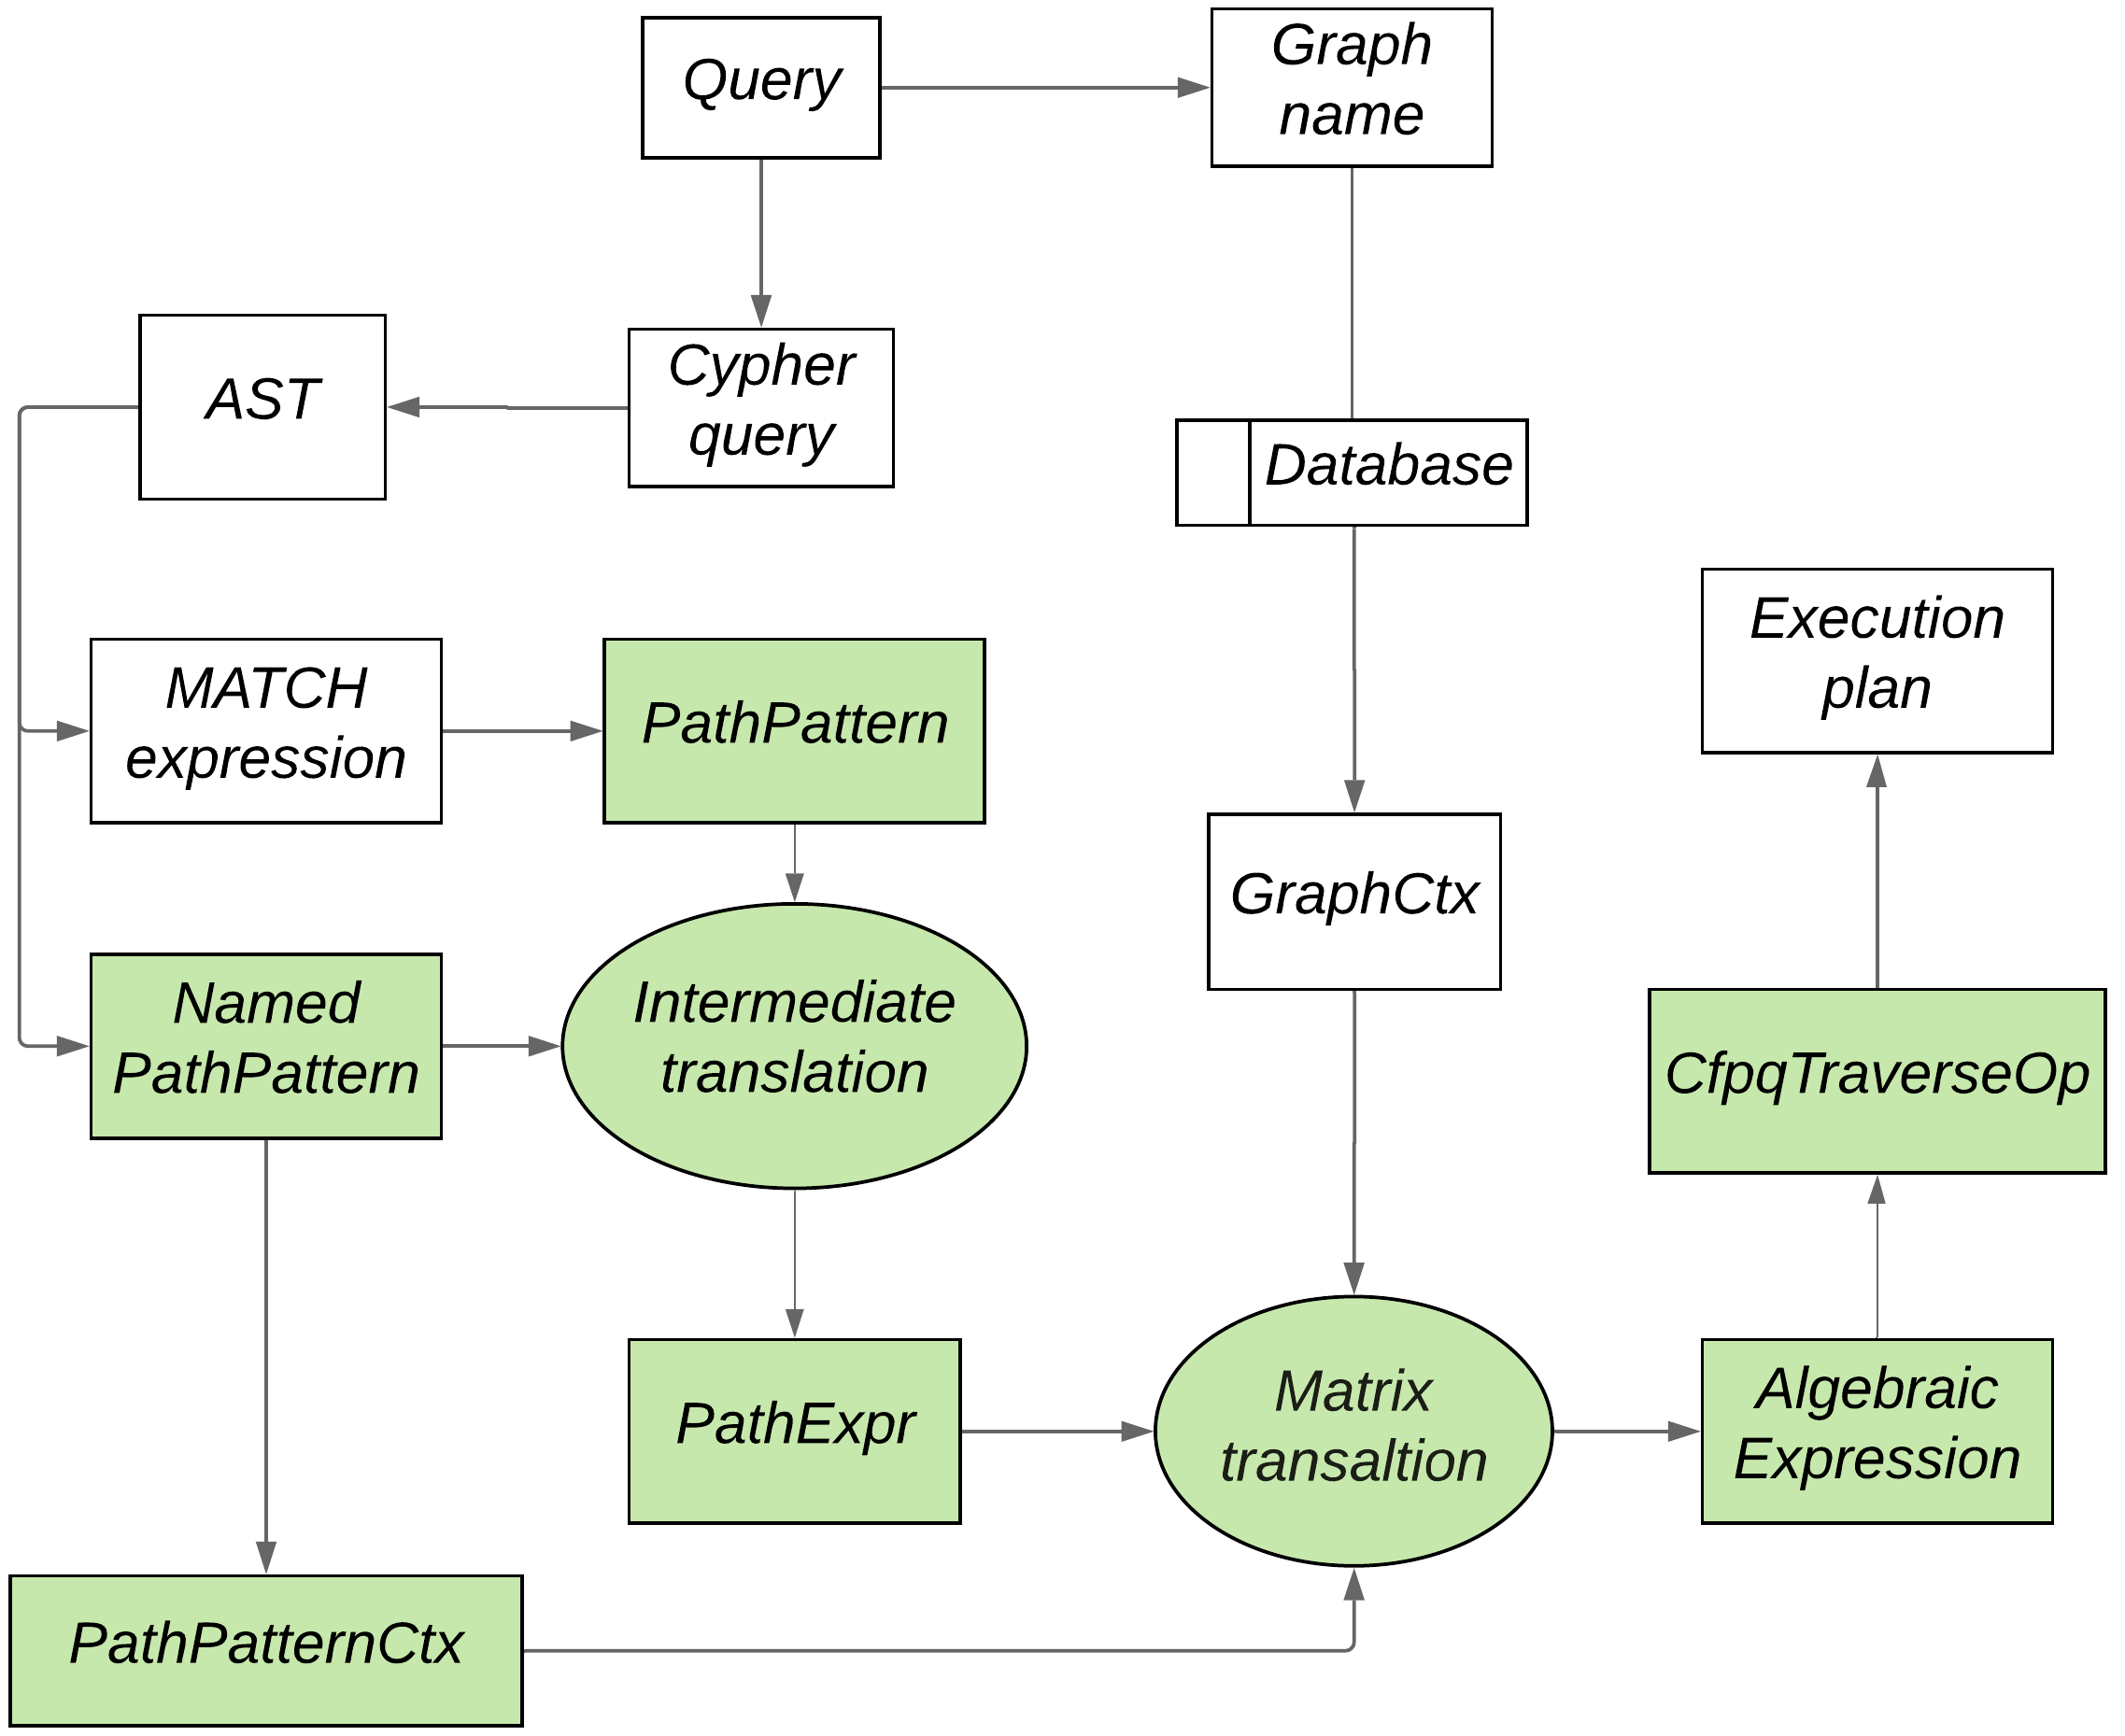
\includegraphics[width=1.0\linewidth]{Terekhov/pictures/execution_plan_3.png}
    \caption{Расширение построения плана выполнения запроса}
    \label{fig:execution_plan}
\end{figure}

\subsection{Промежуточное представление}\label{matrix-translation}
Шаблоны путей, полученные из \textit{AST}, транслируются в промежуточное представление \textit{PathExpr}. Оно позволяет задавать более простой абстрактный синтаксис, который описан на рисунке~\ref{fig:intermidiate_repr}. 

Таким образом, альтернативе и конкатенации шаблонов соответствуют \textit{PathAlt} и \textit{PathSeq}, \textit{PathGroup} позволяет задавать направление пути и наличие замыкания, а \textit{PathBasic} соответствует либо примитивным шаблонам \textit{PathNode}, \textit{PathEdge} и \textit{PathRef}, либо целому выражению \textit{PathExpr}. Примеры промежуточного представления шаблонов приведены в таблице~\ref{tab:inter_examples}.
\begin{figure}[h!]
\begin{align*}
\begin{split}
PathExpr=~ &PathSeq(PathExpr,~PathExpr)~|\\
           &PathAlt(PathExpr,~PathExpr)~|\\
           &PathGroup(PathBasic, direction, range)
\end{split}\\
\begin{split}
PathBasic=~ &PathNode(label)~|\\
            &PathEdge(type)~~|\\
            &PathRef(name) ~~|\\
            &PathExpr
\end{split}\\
\begin{split}
direction \in ~&\{inbound,~outbound,~bidirectional\}\\
range \in     ~&\{*, \varnothing\}
\end{split}
\end{align*}
\caption{Промежуточное представление PathExpr}
\label{fig:intermidiate_repr}
\end{figure}

\begin{table}[h]
\centering
\begin{adjustbox}{max width=\textwidth}
\begin{tabular}{|c|l|}
\hline
$L_p$                        & \multicolumn{1}{c|}{PathExpr}                                                                                                        \\ \hline
{[}:A :B{]} | (:C)           & \begin{tabular}[c]{@{}l@{}}$PathAlt($\\ $~~~~PathSeq(PathEdge("A"),~PathEdge("B"))$\\ $~~~~PathNode("C")$\\ $)$\end{tabular}         \\ \hline
\textless{}{[}:A $\sim$S{]}* & \begin{tabular}[c]{@{}l@{}}$PathGroup($\\ $~~~~PathSeq(PathEdge("A"),~PathRef("S")),$\\ $~~~~inbound,$\\ $~~~~*,$\\ $)$\end{tabular} \\ \hline
\end{tabular}
\end{adjustbox}
\caption{Примеры промежуточного представления запросов}
\label{tab:inter_examples}
\end{table}

\newpage
\subsection{Трансляция в матричные выражения}
Как было упомянуто ранее, RedisGraph представляет графы в виде разреженных матриц. А именно каждый граф $G$ задаётся следующей тройкой $(A \in M_{n\times n},~lab \in Labels \rightarrow Diag_n,~rel \in RelTypes \rightarrow M_{n \times n})_G$. Здесь $M_{n \times n}$ означает полукольцо булевых матриц, а $Diag_n$ полукольцо диагональных булевых матриц. Матрица $A$ служит матрицей смежности графа, а отображения $lab$ и $rel$ сопоставляют меткам вершин и типам рёбер соответствующие булевы матрицы. Таким образом, ребро $(v, to)$ графа $G$ имеет тип $a$ тогда и только тогда, когда $rel(a)_{v,to} = 1$.  Таким же образом, принадлежность метки $l$ вершине $v$ равносильно $lab(l)_{v,v}=1$.

Любую булеву матрицу $M$, участвующую в задании графа $G(V, E)$, можно рассматривать как отношение на множестве вершин $R(M) = \{(v, to):~M_{v,to}=1\}$. Операциями сложения и умножения в булевом полукольце являются дизъюнкция и конъюнкция. Поэтому умножению матриц $A*B$ соответствует композиция отношений $R(A) \circ R(B)$, сложению $A+B$ соответствует объединение отношений $R(A) \cup R(B)$, а транспонированная матрица $A^T$ соответствует обратному к R(A) отношению $R(A)^{-1}$. Такая взаимосвязь между матричными операциями и отношениями лежит в основе алгоритма трансляции, приведённом на рисунке~\ref{algo:translation}.

Данный алгоритм является рекурсивным и принимает на вход промежуточное представление шаблона пути $expr$, представление графа $g$ и контекст именованных шаблонов путей $pathCtx$. Целевым языком трансляции является простой язык матричных выражений, приведённый на рисунке~\ref{fig:alg-expr}.

Базовым случаем рекурсии являются примитивные шаблоны \textit{Path\-Node}, \textit{PathEdge} и \textit{PathReference}, которые транслируются в операнды матричного выражения. Для первых двух соответствующие матрицы извлекаются из графа с помощью функций \textit{GetLabel\-Matrix} и \textit{GetRelation\-Matrix}. При этом случай $label = \varnothing$ соответствует шаблону пути, состоящему из одной произвольной вершины. Поэтому такой путь задаётся тождественным отношением $R(I)$, где $I$ --- единичная матрица. Для \textit{Path\-Reference} создаётся ссылка на матрицу именованного шаблона, которая будет вычислена на следующем этапе при выполнении алгоритма контекстно-свободной достижимости.

Трансляция для шаблонов \textit{PathSeq} и \textit{PathAlt} происходит одинаковым образом --- сначала происходит трансляция дочерних шаблонов, а потом из полученного результата образуются операции умножения или сложения. Такая трансляция обосновывается семантикой шаблонов альтернативы и конкатенации, приведенной в главе~\ref{subsection:cypher-extention}, и связью отношений с матричными операциями, описанными раннее.

Наиболее интересным случаем является трансляция \textit{Path\-Group}, так как в некоторых случаях контекст именованных шаблонов $pathCtx$ расширяется. В начале происходит трансляция дочернего шаблона. Далее, если заданное направление является обратным, к полученной матрице применяется операция транспонирования. Если же направление является произвольным, то формируется операция сложения из полученной матрицы и транспонированной к ней. Это соответствует альтернативе между прямым путём и обратным к нему. После этого при отсутствии замыкания результат возвращается. Иначе происходит трансляция замыкания полученного выражения. Так как его нельзя выразить через имеющиеся матричные операции, создаётся новый именованный шаблон, а замыкание заменяется ссылкой на него. Нетрудно показать, что регулярное выражение $R^*$ и контекстно-свободная грамматика с одним правилом $S \rightarrow R~S \mid \epsilon$ равносильны. Поэтому правая часть этого правила тривиальным образом сразу же транслируется в выражение \textit{Add(Mul(R, MatrixRef(S)), I)} и добавляется в \textit{pathCtx} вместе с полученным новым именем.

Таким образом, после работы данного алгоритма из промежуточного представления шаблона пути получается выражение над матрицами. При дальнейшем его вычислении получается матрица, которая соответствует такому же отношению на множестве вершин, как и семантика изначального шаблона.

\algnewcommand\algorithmicswitch{\textbf{switch}}
\algnewcommand\algorithmiccase{\textbf{case}}
\algnewcommand\algorithmicof{\textbf{of}}
\algnewcommand\algorithmicassert{\texttt{assert}}
\algnewcommand\algorithmiccasepart{\texttt{:}}
\algnewcommand\Assert[1]{\State \algorithmicassert(#1)}%
% New "environments"
\algdef{SE}[SWITCH]{Switch}{EndSwitch}[1]{\algorithmicswitch\ #1}{\algorithmicend\ \algorithmicswitch}%
\algdef{SE}[CASE]{Case}{EndCase}[1]{\algorithmiccase\ #1\algorithmiccasepart}{\algorithmicend\ \algorithmiccase}%
\algdef{SE}[CASEPART]{CasePart}{EndCasePart}[1]{#1\algorithmiccasepart}{\algorithmicend\ \algorithmiccasepart}%
\algtext*{EndSwitch}%
\algtext*{EndCase}%
\algtext*{EndCasePart}%

\begin{algorithm}
\caption{Алгоритм трансляции}
\begin{algorithmic}[1]
\Function{translate}{PathExpr expr, GraphCtx g, PathPatternCtx pathCtx}
    \Switch{expr}
        \Case{$PathNode$(label)}
            \If{label $== \varnothing$}
                \State \Return \Call{GetIdentityMatrix}{g}
            \Else
                \State \Return \Call{GetLabelMatrix}{g, label}
            \EndIf
        \EndCase
        \Case{$PathEdge$(type)}
            \State \Return \Call{GetRelationMatrix}{g, type}
        \EndCase
        \Case{$PathRef(name)$}
            \State \Return $MatrixRef$(name)
        \EndCase
        \Case{$PathSeq$(left, right)}
            \State \Return Add(\Call{translate}{left}, \Call{translate}{right})
        \EndCase
        \Case{$PathAlt$(left, right)}
            \State \Return Mul(\Call{translate}{left}, \Call{translate}{right})
        \EndCase
        \Case{$PathGroup$(basic, dir, range)}
            \State res = \Call{translte}{basic}
            \Switch{dir}
                \Case{$inbound$}
                    \State res = $Transpose$(res)
                \EndCase
                \Case{$bidirectional$}
                    \State res = $Add$(res, $Transpose$(res))
                \EndCase
            \EndSwitch
            \Switch{range}
                \Case{ $\varnothing$}
                    \State \Return res
                \EndCase
                \Case{$*$}
                    \State name = \Call{AllocateNewPathPattern}{ctx}
                    \State res = $Mul$(res, $MatrixRef$(name))
                    \State res = $Add$(res, \Call{GetIdentityMatrix}{g})
                    \State \Call{SetPathPetternExpression}{p, name, res}
                    \State \Return $MatrixRef$(name)
                \EndCase
            \EndSwitch
        \EndCase
    \EndSwitch
\EndFunction
\end{algorithmic}
\caption{Алгоритм транслции в матричные выражения}
\label{algo:translation}
\end{algorithm}

\begin{figure}[H]
\begin{align*}
\begin{split}
AlgExpr= ~ &Add(AlgExpr, AlgExpr)~|\\
           &Mul(AlgExpr, AlgExpr)~|\\
           &Transpose(AlgExpr)~|\\
           &Matrix~|\\
           &MatrixRef(ref)
\end{split}
\end{align*}
\caption{Алгебраическое выражение над матрицами}
\label{fig:alg-expr}
\end{figure}

\subsection{Формирование и вычисление операции плана выполнения}
После этапа трансляции в RedisGraph происходит построение плана выполнения запроса. Он формируется из последовательности операций, которые выполняют базовые вычисления. Для поддержки шаблонов путей была добавлена операция \textit{CfpqTraverseOp}. Она создаётся для каждого матричного выражения, полученного на предыдущем шаге из неименованого шаблона пути, и отвечает за его вычисление.

На этапе инициализации новой операции \textit{CfpqTraverseOp} из соответствующего матричного выражения рекурсивно извлекаются все ссылки на именованные шаблоны путей, от которых зависит данное выражение. После этого они поступают на вход алгоритма, решающего задачу контекстно-свободной достижимости (см. алгоритм 4).

Этот алгоритм является расширенной версией матричного алгоритма Рустама Азимова, приведенного в главе~\ref{sec:matrix-algo}. В данном алгоритме, в отличие от алгоритма Рустама Азимова, не требуется задавать правила грамматики в ослабленной нормальной форме Хомского. Вместо этого правая часть правила задаётся с помощью промежуточного представления \textit{PathExpr}. При этом подразумевается, что для любого именованного шаблона $p$ из глобального контекста \textit{pathCtx} его промежуточное представление уже транслировано в матричное выражение и записано в \textit{pathCtx[p].algExpr}.

Принцип работы алгоритма остаётся прежним. На каждой итерации для всех невычисленных шаблонов происходит вычисление матричного выражения. Если результирующая матрица не изменяется, то она является окончательной для данного именованного шаблона и он больше не участвует в обновлении. Иначе соответствующая матрица перезаписывается.

После работы данного алгоритма все ссылки на именованные шаблоны путей в матричном выражении заменяются на подсчитанные алгоритмом матрицы, после чего происходит вычисление матричного выражения. Результат сохраняется в операции $CfpqTraverseOp$ и участвует в вычислении плана выполнения запроса наряду с результатами других операций. 
\begin{algorithm}
\begin{algorithmic}[1]
\Function{CfpqTraverseNew}{String[] patterns, PathPatternCtx pathCtx}
\While{$\exists$ p $\in$ patterns: !pathCtx[p].isEvaluated}
    \ForAll{p $\in$ patterns}
        \If{!pathCtx[p].isEvaluated}
            \State new\_matrix = \Call{EvalueteAlgExpr}{pathCtx[p].expr}
            \If{new\_matrix == pathCtx[p].matrix}
                \State pathCtx[p].isEvaluated = true
            \Else
                \State pathCtx[p].matrix = new\_matrix
            \EndIf
        \EndIf
    \EndFor
\EndWhile
\EndFunction
\end{algorithmic}
\label{algo:matrix-extention}
\caption{Расширенный матричный алгоритм}
\end{algorithm}


\section{Замеры производительности}
После реализации поддержки нового синтаксиса шаблонов путей были произведены замеры производительности.

\subsection{Сравнение с парсер-комбинаторами}\label{sec:parse-comp-compare}
Сравнительный анализ времени работы полученного решения (колонка RedisGraph) и библиотеки парсер-комбинаторов (колонка Meer\-kat), описанной в главе~\ref{sec:pareser-combinators}, приведён в таблице~\ref{tab:combinators-vs-redisgraph}. Запросы были взяты из эксперимента оригинальной статьи про парсер-комбинаторы~\cite{parser-combinators}. Эквивалентные им запросы, написанные в расширенном синтаксисе Cyp\-her, приведены на рисунках~\ref{code:sub_clas_of_1},~\ref{code:sub_clas_of_2} и представляют из себя частный случай запросов поиска объектов, лежащих на одном уровне иерархии. Набор графов также был взят из вышеупомянутого эксперимента и впервые был представлен в статье Сяованга Чжана~\cite{zhlang-2016}.

% \gsv{У Вас в тексте минимум два разных варианта написания названия этой библиотеки. Надо бы узнать, как правильно и унифицировать}
% \gsv{ лежащих на одном уровне в иерархии}

Замеры обоих решений производились локально на оборудовании со следующими характеристиками: Intel Core i7 4$\times$1.8GHz, 8 GB RAM. Каждый запрос запускался 20 раз и время его работы усреднялось. Время работы указано в миллисекундах. Также в колонках $|V|$ и $|E|$ указано количество вершин и рёбер графа, а в колонке $\#result$ количество найденных соответствующим запросом пар вершин. 

\begin{table}[h!]
\begin{adjustbox}{max width=\textwidth}
\begin{tabular}{|l|c|c|c|c|c|c|c|c|}
\hline
\multicolumn{1}{|c|}{\multirow{2}{*}{$G$}}                   & \multirow{2}{*}{$|V|$} & \multirow{2}{*}{$|E|$} & \multicolumn{3}{c|}{Query\_1}                                                                                                           & \multicolumn{3}{c|}{Query\_2}                                                                                                           \\ \cline{4-9} 
\multicolumn{1}{|c|}{}                                       &                        &                        & \#result & \begin{tabular}[c]{@{}c@{}}Meerkat\\ time (ms)\end{tabular} & \begin{tabular}[c]{@{}c@{}}RedisGraph\\ time (ms)\end{tabular} & \#result & \begin{tabular}[c]{@{}c@{}}Meerkat\\ time (ms)\end{tabular} & \begin{tabular}[c]{@{}c@{}}RedisGraph\\ time (ms)\end{tabular} \\ \hline
wine                                                         & 773                    & 2450                   & 66572    & 541                                                         & 31                                                             & 133      & 6                                                           & 3                                                              \\ \hline
pizza                                                        & 671                    & 2604                   & 56195    & 476                                                         & 24                                                             & 1262     & 30                                                          & 4                                                              \\ \hline
\begin{tabular}[c]{@{}l@{}}measure-\\ primitive\end{tabular} & 341                    & 771                    & 15156    & 158                                                         & 11                                                             & 2871     & 39                                                          & 5                                                              \\ \hline
funding                                                      & 778                    & 1480                   & 17634    & 99                                                          & 14                                                             & 1158     & 14                                                          & 6                                                              \\ \hline
\begin{tabular}[c]{@{}l@{}}atom-\\ primitive\end{tabular}    & 291                    & 685                    & 15454    & 102                                                         & 10                                                             & 122      & 53                                                          & 3                                                              \\ \hline
\begin{tabular}[c]{@{}l@{}}people-\\ pets\end{tabular}       & 337                    & 834                    & 9472     & 55                                                          & 7                                                              & 37       & 3                                                           & 3                                                              \\ \hline
travel                                                       & 131                    & 397                    & 2449     & 21                                                          & 3                                                              & 63       & 2                                                           & 2                                                              \\ \hline
\end{tabular}
\end{adjustbox}
\caption{Сравнение Meerkat и полученного решения}
\label{tab:combinators-vs-redisgraph}
\end{table}

\begin{figure}[h!]
\begin{adjustbox}{max width=\textwidth}
\begin{lstlisting}[language=sql]
PATH PATTERN S = ()-/ [<:Type     [~S | ()] :Type] | 
                      [<:SubClass [~S | ()] :SubClass] /-()
MATCH (v)-/ ~S /->(to)
RETURN COUNT(*)
\end{lstlisting}
\end{adjustbox}
\caption{Query\_1}
\label{code:sub_clas_of_1}
\end{figure}

\begin{figure}[h!]
\begin{adjustbox}{max width=\textwidth}
\begin{lstlisting}[language=sql]
PATH PATTERN S = ()-/ :SubClass | [<:SubClass ~S :SubClass] /-()
MATCH (v)-/ ~S /->(to)
RETURN COUNT(*)
\end{lstlisting}
\end{adjustbox}
\caption{Query\_2}
\label{code:sub_clas_of_2}
\end{figure}

По результатам замеров видно, что даже на небольших графах время работы Meerkat сильно больше, чем время работы полученного решения. При этом в большинстве случаев оно отличатся на порядок. Также стоит отметить, что запросы, указанные на рисунках~\ref{code:sub_clas_of_1},~\ref{code:sub_clas_of_2}, помимо расширенного синтаксиса используют и оригинальную часть языка Cyp\-her, а конкретно функцию COUNT. Это является небольшим примером того, что расширение языка запросов является полностью совместимым с его оригинальной частью.

% Эксперимент, проведенный в статье про парсер-комбинаторы, описанные в  был повторён локально на оборудовании с характеристиками.
% Каждое матричное выражение, полученное при трансляции шаблонов путей, формирует операцию плана выполнения запроса $CfpqTraverse$.

\subsection{Сравнение с матричным алгоритмом}
Графы, приведенные в предыдущих замерах являются достаточно маленькими, поэтому также были произведены замеры на более больших графах. Они были взяты из набора данных CFPQ\_Data~\cite{cfpq-data}, собранного исследователями лаборатории языков инструментов JetBrains Research. Замеры производились таким же образом и на том же оборудовании, что и в главе~\ref{sec:parse-comp-compare}.

% \gsv{Кажется, что нет. go  и прочие большие графы уже просто из нашего набора данных CFPQ\_Data, у китайцев их не было.}

Кроме этого, для анализа издержек выполнения запроса в таблице~\ref{tab:combinators_vs_redisgraph} приводится время работы оригинального алгоритма Рустама Азимова (колонка Matrix algorithm), описанного в главе~\ref{sec:matrix-algo}. Данный алгоритм был интегрирован в RedisGraph и запускался на графах, находящихся в его хранилище. Для этого была разработана отдельная команда, принимающая на вход название графа и путь до файла с грамматикой, написанной в нормальной форме Хомского. Для вычисления матричных операций также использовалась библиотека SuiteSparse.

Таким образом, во-первых, время работы оригинального алгоритма не включает в себя издержки, возникающие при выполнении запроса внутри графовой базы данных. Во-вторых, оригинальный алгоритм отличается от алгоритма, используемого при выполнении запроса в расширенном синтаксисе. Тем не менее время работы обоих решений отличается не сильно и является достаточно небольшим для применения на практике.
\begin{table}[h!]
\begin{adjustbox}{max width=\textwidth}
\begin{tabular}{|l|c|c|c|c|c|c|c|c|}
\hline
\multicolumn{1}{|c|}{\multirow{2}{*}{$G$}} & \multirow{2}{*}{$|V|$} & \multirow{2}{*}{$|E|$} & \multicolumn{3}{c|}{Query\_1}                                                                                                                      & \multicolumn{3}{c|}{Query\_2}                                                                                                                      \\ \cline{4-9} 
\multicolumn{1}{|c|}{}                     &                        &                        & \#result & \begin{tabular}[c]{@{}c@{}}Matrix\\ algorithm\\ time (ms)\end{tabular} & \begin{tabular}[c]{@{}c@{}}RedisGraph\\ time (ms)\end{tabular} & \#result & \begin{tabular}[c]{@{}c@{}}Matrix\\ algorithm\\ time (ms)\end{tabular} & \begin{tabular}[c]{@{}c@{}}RedisGraph\\ time (ms)\end{tabular} \\ \hline
go                                         & 272770                 & 1068622                & 304070   & 1272                                                                   & 1236                                                           & 334850   & 662                                                                    & 683                                                            \\ \hline
go-hierarchy                               & 45007                  & 1960436                & 588976   & 271                                                                    & 276                                                            & 738937   & 193                                                                    & 290                                                            \\ \hline
eclass-514                                 & 48815                  & 219390                 & 90994    & 198                                                                    & 304                                                            & 96163    & 121                                                                    & 241                                                            \\ \hline
enzyme                                     & 239111                 & 1047454                & 396      & 103                                                                    & 47                                                             & 8163     & 68                                                                     & 37                                                             \\ \hline
\end{tabular}
\end{adjustbox}
\caption{Сравнение матричного алгоритма и полученного решения}
\label{tab:combinators_vs_redisgraph}
\end{table}

\subsection{Сравнение с анализом Йохема Куйперса}
Также был произведён замер времени работы на очень большом графе geospeices~\cite{geospices}. Этот граф является довольно важным, потому что он участвовал в сравнительном анализе алгоритмов, проведенным Йохемом Куйперсом. Именно из-за колоссального времени работы запроса на данном графе дальнейшее расширение языка запросов Йохемом Куйперсом и др. было приостановлено. 

Повторить эксперимент не предоставилось возможным, так как в статье не приводились ссылки на реализацию алгоритмов. Поэтому в таблице~\ref{tab:neo4j-vs-redisgraph} приводится замер из оригинальной статьи алгоритма с наилучшим временем работы (колонка Neo4j). Время указано в секундах. Эквивалентный запрос в расширенном синтаксисе приводится на рисунке~\ref{code:broaderTransitive}. Характеристики оборудования, на которых выполнялись запросы, следующие:

\begin{itemize}
    \item Neo4j: Intel Xeon E5-4610 v2, 8$\times$2.30GHz, 400 GB RAM
    \item RedisGraph: Intel Core i7-6700 CPU, 64 GB RAM 4$\times$3.4GHz
\end{itemize}

\begin{figure}[h!]
\begin{adjustbox}{max width=\textwidth}
\begin{lstlisting}[language=sql]
PATH PATTERN S = ()-/ [:broaderTransitive [~S | ()] <:broaderTransitive] /-()
MATCH (v)-/ ~S /->(to)
RETURN COUNT(*)
\end{lstlisting}
\end{adjustbox}
\caption{Query}
\label{code:broaderTransitive}
\end{figure}

\begin{table}[h!]
\begin{adjustbox}{max width=\textwidth}
\begin{tabular}{|l|c|c|c|c|c|}
\hline
\multicolumn{1}{|c|}{G} & $|V|$   & $|E|$     & \#result    & \begin{tabular}[c]{@{}c@{}}Neo4j\\ time (s)\end{tabular} & \begin{tabular}[c]{@{}c@{}}RedisGraph\\ time (s)\end{tabular} \\ \hline
geospeices              & 225 000 & 1 550 000 & 226 669 749 & 6 953.9                                                       & 26.1                                                          \\ \hline
\end{tabular}
\end{adjustbox}
\caption{Сравнение с замером Йохема Куйперса}
\label{tab:neo4j-vs-redisgraph}
\end{table}

По результатам замеров видно, что удалось достичь времени работы в десятки секунд. Такое время было обозначено Куйперсом как приемлемое время работы для практического применения.

% \gsv{а значит .... Закончите мысль выводом.} 

\subsection{Выводы}
По результатам замеров времени выполнения можно говорить о том, что полученное решение делает запросы с контекстно-свободными ограничениями доступными для практического применения. При этом новый синтаксис языка сильно расширяет его возможности и является полностью совместимым с его оригинальной версией.

\section*{Заключение}
В ходе работы были получены следующие результаты:
\begin{itemize}
\item Выполнен обзор текущих решений поддержки запросов с кон\-текстно-свободными ограничениями, по результатам которого было решено интегрировать матричный алгоритм Рустама Азимова в графовую базу данных RedisGraph с последующим расширением языка запросов Cypher. 
\item Интегрирован матричный алгоритм Рустама Азимова в RedisGraph.
\item Разработана поддержка расширения языка запросов Cypher для RedisGraph, позволяющая задавать запросы с конте\-кстно-сво\-бод\-ными ограничениями. Исходный код находится в репозитории на github~\cite{github}. Также для удобства и возможности позапускать запросы без процесса установки необходимого программного обеспечения предоставляется docker контейнер~\cite{docker}.
\item Произведены замеры производительности полученного решения и сравнение времени работы с текущими аналогами.
\item Результаты работы изложены в статье, принятой на конференцию GRADES-NDA 2020.
\end{itemize}

В будущем планируется разработать подробную пользовательскую документацию запросов в расширенном синтаксисе, так как черновой вариант официальной спецификации рассчитан больше на разработчиков. Также планируется отправить запрос на принятие изменений в официальный репозиторий RedisGraph. 

%\setmonofont[Mapping=tex-text]{CMU Typewriter Text}
%\bibliographystyle{ugost2008ls}
%\bibliography{diploma.bib}
%\end{document}

\section{Обзор}

% ------------- Обзор предметной области ---------------

\subsection{Символьное исполнение}\label{symbolicExec}
\emph{Символьное исполнение}~--- техника, которая позволяет исполнять программный код в условиях неопределённости входных данных, исследуя все ветки выполнения программы. При конкретном исполнении функции из \autoref{example3}, условие $(\texttt{x} > \texttt{y})$ будет либо ложным, либо истинным, следовательно будет выполнена только одна ветка. При символьном исполнении этой функции входные данные (т. е. \texttt{x} и \texttt{y}) будут заменены на \emph{символы}~--- абстракции над конкретными значениями, при этом обе эти ветки будут исполнены, а результат исполнения каждой ветки будет защищен соответствующим условием попадания в неё. Такое условие будем называть \emph{условием пути}.

Условие пути является одним из элементов состояния интерпретатора, в которое также входит и \emph{символьная память}~--- представление состояния памяти при символьном исполнении. В начале исследования функции условие пути равно \texttt{true}. При встрече ветвления текущая ветка исполнения разбивается на две, условия пути которых равны условиям попадания в ветку \texttt{then} и \texttt{else} соответственно.

\begin{listing}[H]
\begin{lstlisting}[language=csharp]
public static int MaxInt(int x, int y) {
    int maxInt = 0;
    if (x > y) {
        maxInt = x;
    }
    else {
        maxInt = y;
    }
    return maxInt;
}
\end{lstlisting}
\caption{Пример функции для символьного исполнения}
\label{example3}
\end{listing}

Одним из видов символьного исполнения является \emph{статическое символьное исполнение}, результатом которого является значение, которое вернула функция, а также состояние символьной памяти. Главной особенностью данного вида является \emph{слияние} результатов исполнения веток, полученных разветвлении одной ветки. После слияния получается результат исполнения (т. е. значение и символьная память), вбирающий в себя все изначальные ветки, полученный благодаря введению новых синтаксических конструкций, например $ite(condition, thenTerm, elseTerm)$. Результатом исполнения функции из примера в таком случае будет значение $ite(\texttt{X} > \texttt{Y}, \texttt{X}, \texttt{Y})$ и символьная память $M=\{ \texttt{x}\mapsto \texttt{X}, \texttt{y}\mapsto \texttt{Y}, \texttt{maxInt}\mapsto ite(\texttt{X} > \texttt{Y}, \texttt{X}, \texttt{Y}) \}$, где \texttt{X} и \texttt{Y} являются символьными значениями переменных \texttt{x} и \texttt{y} соответственно. 

Для назначения входным данным символьных значений может использоваться метод \emph{ленивой инстанциации}~\cite{khurshid2003generalized} (англ. lazy instantiation). Главная идея данного метода заключается в инициализации данных по необходимости, т. е. вначале символьного исполнения функции все входные данные помечаются как неинициализированные. При первом использовании таких данных происходит их инициализация. Если инициализируется переменная ссылочного типа, то в неё недетерминированно помещаются: значение \texttt{null}, ссылка на новый объект с неинициализированными полями, ссылка на ранее созданный объект. В случае инициализации переменной простого типа, в неё помещается символьное значение соответствующего ей типа. В данном методе во время инициализации значений используется условие пути для проверки, что полученное значение может находиться в данной переменной. Благодаря такому подходу возможно символьное исполнение в условиях отсутствия знаний о некоторых простых ссылочных локациях (т. е. ссылочных локациях у которых известное количество полей). В частности, это позволяет исследовать функции с некоторыми рекурсивными структурами данных без указания априорных ограничений на их размер.

Одним из главных минусов техники символьного исполнения является \emph{взрыв путей исполнения}, т. е. экспоненциальный рост количества исследуемых веток. Важно отметить, что некоторые из этих веток могут быть недостижимы, условия пути в таких ветках будут невыполнимыми.

Для проверки достижимости веток выполнения современные верификаторы~\cite{sethu2018systems, yoshida2017klover, sharma2018veritesting} используют SMT-решатели, которые могут проверять, выполнима ли формула пути определённой ветки: если нет, то исполнение такой ветки прекращается.

\subsection{SMT-решатели}\label{smt}

SMT-решатели~\cite{de2008z3, barrett2011cvc4} являются инструментами для автоматизированной проверки выполнимости логических формул в теориях. На вход эти инструменты принимают формулу логики первого порядка с функциональными, предикатными и константными символами из сигнатуры заранее заданных теорий. Если формула выполнима, то в качестве результата решатель возвращает \texttt{SAT}\footnote{Выполнима (англ. satisfiable)} и модель, которая интерпретирует формулу истинно. Если формула невыполнима, и решателю удалось это доказать, то он возвращает \texttt{UNSAT}. Помимо этих результатов, решатель может вернуть \texttt{UNKNOWN} или зависнуть, так как некоторые теории или их комбинации являются неразрешимыми.

Среди теорий, поддерживаемых решателями, можно выделить следующие: теория линейной целочисленной арифметики, линейной вещественной арифметики, неинтерпретированных функций, а также массивов.

\emph{Теория линейной целочисленной арифметики.} Сигнатура данной теории включает в себя целые числа, операции сложения и вычитания, а также предикаты равенства и меньше. Данная теория является разрешимым фрагментом арифметики.

\emph{Теория линейной вещественной арифметики.} Сигнатура данной теории логики первого порядка содержит вещественные числа, операции сложения и вычитания, предикаты равенства и меньше. Описанная теория является разрешимой.

\emph{Теория нелинейной целочисленной арифметики.} Сигнатура данной теории включает в себя целые числа, операции сложения, вычитания и умножения, а также предикаты равенства и меньше. Данная теория является неразрешимой~\cite{godel1931formal}.

\emph{Теория нелинейной вещественной арифметики.} Сигнатура данной теории логики первого порядка содержит вещественные числа, операции сложения, вычитания и умножения, предикаты равенства и меньше. Описанная теория является разрешимой~\cite{tarski1998decision}.

\emph{Теория битовых векторов.} В сигнатуру данной теории входят числа, каждое из которых представляет битовый вектор фиксированной длины (представления чисел в машинной арифметике), предикаты равенства и меньше, операции сложения и произведения, а также следующие битовые операции: <<и>>, <<или>>, <<исключающее или>>, <<не>>, <<сдвиг влево>>, <<сдвиг вправо>>, <<конкатенация двух бит-векторов>>, <<взятие подвектора>>. Данная теория является разрешимой~\cite{barrett1998decision}, так как сводится к задаче выполнимости формул логики высказываний.

% ------------- Обзор существующих решений ---------------

\subsection{Модели памяти}
\emph{Модель памяти}~\cite{mandrik}~--- это формальное представление указателя и ссылки, а также формализация результата операций над ними c использованием логических формул. Среди существующих на данный момент методов моделирования операций с памятью можно выделить две группы подходов: модели для для высокоуровневого анализа памяти и для низкоуровневого. Далее отдельно отдельно разберём обе эти группы подходов. Более подробный обзор существующих моделей памяти приведён в статье~\cite{mandrik}.

\subsubsection{Модели высокоуровневого анализа памяти}

Модели высокоуровневого анализа памяти направлены на анализ рекурсивных структур данных заранее неогрниченного размера, однако в общем случае не поддерживают массивы, адресную арифметику и приведения типов указателей. Среди таких моделей выделим \textsc{LISBQ}~\cite{lahiri2008back}.

\paragraph{LISBQ.} Данный способ моделирования операций с памятью основан на LISBQ (Logic of Interpreted Sets and Bounded Quantification)~--- логике интерпретируемых множеств и ограниченной квантификации. Этот метод используется в дедуктивной верификации, например, в инструменте \textsc{HAVOC}~\cite{bornat2000proving}. Для моделирования поведения программы в логике первого порядка модель памяти LISBQ использует теорию линейной целочисленной и вещественной арифметики. Главными минусами данной модели являются отсутствие поддержки массивов, адресной арифметики, приведений типов указателей. Помимо этого основной особенностью этого метода является необходимость аннотаций со стороны пользователя для достижения \emph{точного анализа} (т. е. порождаемые формулы описывают все поведения программы и только их), что влечёт неприменимость данной модели для автоматизированного анализа.

\subsubsection{Модели низкоуровневого анализа памяти}

Модели памяти, выполняющие низкоуровневый анализ памяти, в отличие от моделей высокоуровневого анализа памяти, сфокусированы на анализе массивов, приведении типов указателей, адресной арифметики, однако не поддерживают произвольные свойства рекурсивных структур данных. Первой среди таких моделей рассмотрим \emph{модель памяти на основе анализа алиасов}.

\paragraph{Модель памяти на основе анализа алиасов~\cite{andersen1994program}.} Данный метод моделирования операций с памятью выполняет анализ синонимичных указательных выражений, что позволяет находить указатели, которые могут ссылаться на одну область памяти. Такая модель памяти была использована в инструменте автоматической верификации \textsc{BLAST}~\cite{beyer2007software}. Данный метод ориентирован на области памяти заранее ограниченного размера (например, структуры или значения простых типов). Однако области памяти заранее неограниченного размера (например, массивы переменной длины) в общем случае не поддерживаются, а именно не поддерживается проверка произвольных свойств таких областей~\cite{mandrik}. Также необходимо отметить, что проверка некоторых простых свойств рекурсивных структур данных может быть выполнена в рамках данной модели.
Для кодирования в SMT-решатель этот метод использует теории линейной вещественной арифметики и неинтерпретированных функций. Формулы, порождаемые данным методом, которые моделируют результат операций с памятью, описывают упрощенный результат, дополненный ложными знаниями, из-за чего происходят многочисленные ложные срабатывания. Данная особенность говорит о неприменимости такого моделирования для задачи проверки произвольных свойств программы. Помимо этого, модель памяти с использованием анализа алиасов не подходит для проверки произвольных свойств программ платформы \dotnet{}, так как в этих программах можно выделить область памяти заранее не ограниченного размера (например, массив). Для анализа памяти таких программ используются модели для областей памяти заранее неограниченного размера, среди которых \emph{типизированная модель}.

\paragraph{Типизированная модель~\cite{cohen2009precise}.} Основной идеей данной модели, используемой в дедуктивной верификации, является сужение области возможных локаций, на которые может указывать указатель, благодаря знаниям о типе локаций и указателя. Если типы локации и указателя совпадают, то указатель может указать на данную локацию. Такая информация о типах предоставляется при помощи аннотаций пользователя, что означает неприменимость для автоматизированной верификации. Такая модель памяти была реализована в инструменте дедуктивной верификации VCC2~\cite{cohen2009vcc}. Для моделирования операций с памятью в логике первого порядка типизированная модель памяти использует следующие теории: теорию массивов, линейной целочисленной и вещественной арифметики. Главным недостатком данной модели является отсутствие поддержки произвольных свойств рекурсивных структур данных. Помимо этого, данный метод ориентирован на дедуктивную верификацию, а значит неприменим в автоматической верификации. Улучшением этого метода моделирования операций с памятью является \emph{модель Бурсталла-Борната}.

\paragraph{Модель Бурсталла-Борната~\cite{bornat2000proving}.} Главной идеей данного способа моделирования, применяемого в области частично автоматизированной дедуктивной верификации, является раздельное представление состояния памяти для компонентов составных объектов, иначе говоря, вся моделируемая память программы является массивом, элементы которого~--- это элементы составных объектов. В качестве теорий логики первого порядка для моделирования поведения программы данная модель использует те же теории, что и типизированная модель памяти, т. е. теорию массивов, линейной целочисленной и вещественной арифметики. Основной особенностью такого метода является достижение точного анализа путём требования аннотаций со стороны пользователя, что неприменимо в случае автоматической верификации. Отсутствие поддержки произвольных свойств рекурсивных структур данных, как и в случае с типизированной моделью, является основным минусом. Расширением такой модели памяти является \emph{модель памяти с регионами}.

\paragraph{Модель памяти с регионами~\cite{hubert2007separation}.} Ключевой идеей данной модели памяти для дедуктивной верификации является уменьшение пространства возможных локаций для определённого указателя с помощью добавления понятия \emph{регионов}. \emph{Регионы}~--- такие непересекающиеся множества указательных выражений, что элементы из разных множеств не могут адресовать пересекающиеся области в памяти. Последняя модификация данной модели была представлена в работе~\cite{mandrykin2017memory} М.~У.~Мандрыкина и А.~В.~Хорошилова. Модель памяти с регионами, как и модель Бурсталла-Борната, использует теорию массивов, линейной целочисленной и вещественной арифметики для моделирования операций программы с памятью. Данная модель относится к моделям памяти для дедуктивной верификации, т. е. основывается на аннотациях пользователя, что невозможно в случае автоматической верификации. Недостатки данной модели типичны для моделей низкоуровневого анализа памяти, т. е. отсутствует поддержка произвольных свойств рекурсивных структур данных~\cite{mandrik}.

\section{Метод описания путей в графе потока управления}
В данном разделе будет описана формальная теория, необходимая для нового алгоритма композиционального символьного исполнения, который не раскручивает отношение перехода. Основной объект~--- это способ описания всех путей в графе потока управления, начинающихся из стартовой вершины, с использованием механизма введения \emph{рекурсивных символов для множества путей}, которые будут соответствовать \emph{рекурсивным символам куч} $\GRec{\cdot}$ из определения обобщенных куч. Метод похож на интервальный анализ графов, но распространяется на случай \emph{нередуцируемых} графов.
Необходимо ввести минимальное количество таких символов, чтобы не затруднять будущую работу нижележащего решателя, но в то же время сохранить полноту и корректность описания путей.

\begin{defn}
Граф потока управления --- это четверка ($V_G$, $E_G$, $start$, $exit$), где:
\begin{itemize}
    \item $V_G$ --- это множество вершин графа, каждая из которых соответствует инструкции программы;
    \item $E_G$ --- это множество ориентированных ребер $e = (u, v)$ графа, каждое ребро обозначает способность передачи управления от вершины $u$ к вершине $v$;
    \item $start$ --- это стартовая вершина (инструкция), в которую не входит ни одно ребро графа;
    \item $exit$ --- это финальная вершина (инструкция), из которой не выходит ни одного ребра графа.
\end{itemize}
\end{defn}

\subsection{Основные понятия}
Для произвольного графа потока управления, построенного по программе,
занумеруем вершины при помощи обратного обхода (Post Order DFS), который присваивает каждой вершине время посещения по формуле:
$$time(v) = |V_G| - |\{u \in V_G| \mbox{для вершины u уже вычислено time(u)}\}|.$$

\begin{defn}\label{backEdges}
Ребро $e = (u,v)$, соединяющее вершины $u$ \emph{и} $v$, называется \emph{обратным}, если $time(u) \geq time(v)$. 
Если ребро не является \emph{обратным}, то оно называется \emph{прямым}.
Обозначим $beg(e) = u$, а $end(e) = v$.
Множество обратных ребер обозначим $BE$.
\end{defn}

\begin{defn}\label{recursiveVertex}
Вершина $s$ называется \emph{рекурсивной}, если $\exists e \in E_G$, что $e$ --- обратное \emph{и} $end(e) = s$. 
Множество \emph{рекурсивных} вершин обозначим $RV$.
\end{defn}

\begin{defn}
Путем $p$ в графе $G$ будем называть последовательность ребер $e_1...e_n$ такую,
что $\forall i$ $ 1 \leq i \leq n - 1$ $end(e_i) = beg(e_{i+1})$.
Началом пути $beg(p)$ обозначим вершину $beg(e_1)$.
Концом пути $end(p)$ обозначим вершину $end(e_n)$.
Иногда удобно представлять путь в графе в виде последовательности вершин:
$v_1 \ra v_2 \ra ... \ra v_n \ra v_{n + 1}$ такой, что $\forall i$ $1 \leq i \leq n$ $v_i = beg(e_i)$ и $v_{i+1} = end(e_i)$.
\end{defn}

\begin{defn}
Путь, состоящий из 0 ребер, называется \emph{пустым}.
Будем обозначать его $\varepsilon$.
\end{defn}

\begin{defn}
Пусть даны два пути $p_1$ и $p_2$ в графе $G$.
Если $end(p_1) = beg(p_2)$, то можно определить конкатенацию путей $p_1$ и $p_2$, обозначаемую $p_1 \circ p_2$ и представляющую путь, содержащий все ребра пути $p_1$, за которыми следуют ребра $p_2$.

Заметим, что пустой путь $\varepsilon$ является нейтральным элементов по отношению к операции конкатенации.
\end{defn}

\begin{defn}
Дана вершина графа $v$.
Дано множество путей $P_1$, что все пути заканчиваются на вершине $v$.
Дано множество путей $P_2$, что все пути начинаются с вершины $v$.
Тогда определим конкатенацию множеств путей $P_1$ и $P_2$ таким образом:
$$P_1 \circ P_2 = \{p_1 \circ p_2 \quad | \quad p_1 \in P_1, p_2 \in P_2 \}.$$
\end{defn}

\subsection{Метод}
Введем определения, для которых докажем необходимые леммы для получения формулы всех путей в CFG.


\begin{defn}
Если длина пути $p = v_0 \ra v_1 \ra ... \ra v_n \ra v_{n+1}$ больше, либо равна 2, то будем называть серединой пути множество вершин 
$\{v_i \mid 1 \leq i \leq n$\}. Если длина пути меньше 2, то середина пути --- $\varnothing$.
\end{defn}

\begin{defn}
$\Pi(u,v,D)$ --- символ для множества путей, начинающихся в вершине $u$, заканчивающихся в вершине $v$ \emph{и} не проходящих через \emph{рекурсивные}
вершины множества $D$ в середине пути. Это множество путей строится с помощью следующих правил.
\begin{itemize}
    \item Если в графе есть ребро $(u,v)$, то путь, состоящий из одного ребра, добавляется во множество путей $\Pi(u,v,D)$ (см. правило~\ref{eq:I}).
    \item Если есть ребро $(u,t)$, где $t \neq v$ и $t \notin RV$, то конкатенация ребра $(u,t)$ и путей $\Pi(t,v,D)$ добавляется к множеству путей $\Pi(u,v,D)$ (см. правило~\ref{eq:II}).
    \item Если есть ребро $(u,t)$, где $t \neq v$, $t \in RV$ \emph{и} $t \notin D$, то конкатенация ребра $(u,t)$ и $Rec(t,\append{D}{t}) \circ \Pi(t,v,\append{D}{t})$ добавляется к множеству путей $\Pi(u,v,D)$ (см. правило~\ref{eq:III}), где $Rec(t,\append{D}{t})$ --- множество циклов из $t$ в $t$, не проходящих через
    \emph{рекурсивные} вершины из множества $\append{D}{t}$ в середине пути, а $\Pi(t,v,\append{D}{t})$ --- множество путей из $t$ в $v$, не проходящих через \emph{рекурсивные} вершины из множества $\append{D}{t}$ в середине пути. 
\end{itemize}

$Rec(u,D)$ --- рекурсивный символ для множества циклов из вершины $u$ в вершину $u$, не проходящих через вершины из множества $D$ в середине пути, которые построены по правилу~\ref{eq:IV}.
\begin{itemize}
    \item Пустой путь $\varepsilon$ принадлежит множеству $Rec(u,D)$.
    \item Конкатенация путей $\Pi(u,u,D)$ и циклов $Rec(u,D)$ добавляется к множеству циклов $Rec(u,D)$. 
\end{itemize}

\begin{subequations}
    % \begin{empheq}[box=\widefbox]
    \begin{alignat}{1}
    \Pi(u,v,D) = {}  & \bigcup_{(u,v) \in E_G}\{(u,v)\} \qquad \cup \tag{I}\label{eq:I}\\
                     & \bigcup_{\substack{t \notin RV \\ t \neq v \\(u,t) \in E_G}}(u,t) \circ \Pi(t,v,D) \qquad \cup \tag{II}\label{eq:II} \\
                     & \bigcup_{\substack{t \in RV \\ t \neq v \\(u,t) \in E_G \\ t \notin D}}(u,t) \circ Rec(t,\append{D}{t}) \circ \Pi(t,v,\append{D}{t}) \tag{III}\label{eq:III} \\
    Rec(u,D) ={}     & \{\varepsilon\} \cup \Pi(u,u,D) \circ Rec(u,D) \tag{IV}\label{eq:IV}
    \end{alignat}
    % \end{empheq}
\end{subequations}
\end{defn}

\begin{lm}
\label{lemma:evident}
$\forall p \in \Pi(u,v,D)$ начало пути $beg(p) = u$ \emph{и} конец пути $end(p) = v$.
\end{lm}
\begin{proof}
Очевидно.
\end{proof}

\begin{lm}
\label{lemma:length}
$\forall u,v,D$ верно, что $\varepsilon \notin \Pi(u,v,D)$.
\end{lm}
\begin{proof}
Очевидно, поскольку согласно правилам~(\ref{eq:I} -- \ref{eq:III}), любой путь $p \in \Pi(u,v,D)$ начинается с ребра $(u,t)$.
\end{proof}

\begin{lm}
\label{lemma:reduction}
Пусть дан путь $p = s_1 \ra ... \ra s_n$ такой, что $\forall i > 1 \hspace{5mm} s_i \neq s_1$. \\
Тогда $p \in Rec(s_1,D) \circ \Pi(s_1, s_n, D) \iff p \in \Pi(s_1,s_n,D)$.
\end{lm}

\begin{proof}
\emph{Достаточность.} Очевидно, поскольку $\varepsilon \in Rec(s_1,D)$. \\
\emph{Необходимость.} Раскроем определение $Rec(s_1,D)$.\\
\begin{equation}
    \begin{aligned}
    Rec(s_1,D) \circ & \Pi(s_1,s_n,D) = \\ 
                     & \begin{cases} 
            \Pi(s_1,s_n,D) \\
            \Pi(s_1,s_1,D) \circ Rec(s_1,D) \circ \Pi(s_1, s_n,D)
            \end{cases}
    \end{aligned}
\end{equation}
Согласно леммам~\ref{lemma:evident}~,~\ref{lemma:length} $\forall p \in \Pi(s_1, s_1,D) \circ Rec(s_1,D) \circ \Pi(s_1, s_n,D)$
вершина $s_1$ встречается в $p$ как минимум два раза, но по условию, $s_1$ встречается только один раз.
Следовательно, единственная возможность --- $p \in \Pi(s_1,s_n,D)$.
\end{proof}

% \kostya{Дать отдельное определение для длины пути?}
\begin{lm}
\label{lemma:main}
Пусть даны множество $D$ такое, что $D \subseteq RV$, и путь $p = s_1 \ra ... \ra s_n$, удовлетворяющий условиям:
\begin{enumerate}
    \item длина $p \geq 1$;
    \item $s_n = exit$ или $s_n \in D$;
    \item $\forall i < n, \hspace{5mm} s_i \notin D \setminus \{s_1\}$.
\end{enumerate}
% $s_n$ является либо финальной вершиной, либо \emph{рекурсивной} ($s_n \in RV$) и
% $\forall i < n \hspace{5mm} s_i \notin D \setminus \{s_1\} \land s_i = s_n \implies s_i = s_1$.
Тогда верно следующее.
\begin{itemize}
    \item Если $s_1 \notin RV$, то $p \in \Pi(s_1,s_n,D)$.  
    \item Если $s_1 \in RV$, то $p \in Rec(s_1,D) \circ \Pi(s_1,s_n,D)$.  
\end{itemize}
\end{lm}

\begin{proof}
Индукция~\#1 по длине пути $p$. 
База: длина пути равна 1. Тогда $p = s_1 \ra s_n \in \{(s_1,s_n)\} \subseteq \Pi(s_1,s_n,D)$.
Если $s_1 \in RV$, то $p \in Rec(s_1,D) \circ \Pi(s_1,s_n,D)$, поскольку $\varepsilon \in Rec(s_1,D)$.

Индукционный переход.
\begin{itemize}
    \item Пусть $p = s_1 \ra v \ra ... \ra s_n$, и предположим, что вершина $s_1$ встречается в пути $p$ ровно 1 раз.
    \begin{itemize}
        \item Если вершина $v \notin RV$, то по И.П.~\#1, путь $v \ra ... \ra s_n \in \Pi(v,s_n,D)$, и, по правилу~(\ref{eq:II}), имеем $p \in \Pi(s_1,s_n,D)$, 
        так как $v \neq s_n$.
        \item Пусть вершина $v \in RV$. Тогда по условию (3) можно сделать вывод, что $v \notin D$.
        Поскольку для всех вершин $u$, кроме последней, в пути $v \ra ... \ra s_n$ выполнено 
        $u \notin \append{D}{v} \setminus \{v\}$, так как среди них нет $s_1$,
        то по И.П.~\#1, верно, что $v \ra ... \ra s_n \in Rec(v,\append{D}{v}) \circ \Pi(v, s_n,\append{D}{v})$, а значит, по правилу~(\ref{eq:III}), 
        $p \in \Pi(s_1, s_n, D)$, так как $v \neq s_n$.
    \end{itemize}
    Если вершина $s_1 \in RV$, то $p \in Rec(s_1,D) \circ \Pi(s_1,s_n,D)$, поскольку $\varepsilon \in Rec(s_1,D)$.
    
    \item Пусть $p = s_1 \ra v \ra ... \ra s_1 \ra ... \ra s_n$ и $s_1 \in RV$.
          Обозначим $p \equiv q \circ p'$, где $q \equiv s_1 \ra ... \ra s_1$, а
          $p' \equiv s_1 \ra ... \ra s_n$ такой, что вершина $s_1$ встречается в пути $p'$ ровно один раз, если $s_n \neq s_1$, или ровно два раза, если $s_n = s_1$. Если $s_1 \neq s_n$, то по И.П.~\#1, $p' \in Rec(s_1,D) \circ \Pi(s_1,s_n,D)$, откуда по лемме~\ref{lemma:reduction},
          $p' \in \Pi(s_1,s_n,D)$. Если $s_n = s_1$, то рассмотрим подробнее путь $p'$.
          \begin{itemize}
            \item $p' \equiv s_1 \ra s_1$, откуда $q' \in \{(s_1,s_1)\} \subseteq \Pi(s_1,s_1,D)$.
            \item $p' \equiv s_1 \ra v_1 \ra ... \ra v_m \ra s_1$ такой, что $v_1 \notin RV$.
                  Так как $\forall 1 \leq i \leq m$ верно, что $v_i \notin D$, то 
                  по И.П.~\#1, путь $v_1 \ra ... \ra v_m \ra s_1 \in \Pi(v_1, s_1, D)$, а, по правилу~(\ref{eq:II}), получаем, что
                  $p' \in \Pi(s_1,s_1,D)$, так как $v_1 \neq s_1$.
            \item $p' \equiv s_1 \ra v_1 \ra ... \ra v_m \ra s_1$ такой , что $v_1 \in RV$.
                Так как $\forall 1 \leq i \leq m$ верно, что $v_i \notin \append{D}{v_1} \setminus \{v_1\}$, то 
                по И.П.~\#1, путь $v_1 \ra ... \ra v_m \ra s_1 \in Rec(s_1,\append{D}{v_1}) \circ \Pi(v_1,s_n,\append{D}{v_1})$,
                а, по правилу~(\ref{eq:II}), получаем, что $p' \in \Pi(s_1,s_1,D)$, так как $v_1 \neq s_1$.
        \end{itemize}
        Осталось показать, что $q \in Rec(s_1,D)$.
        Индукция~\#2 по длине q. База $q \equiv \varepsilon$ --- очевидно. \\
        Переход. Пусть $q \equiv q' \circ q''$, где $q' \equiv s_1 \ra ... \ra s_1$ и содержит только два вхождения $s_1$, 
        а $q'' \equiv s_1 \ra ... \ra s_1$ является остатком пути $q$.
        Но по И.П.~\#2, получаем, что $q'' \in Rec(s_1, D)$. 
        Аналогично получаем, что $q' \in \Pi(s_1,s_1,D)$. Тогда согласно правилу~(\ref{eq:IV}), получаем, что $q \in Rec(s_1,D)$.
        Но тогда $p \equiv q \circ p' \in Rec(s_1,D) \circ \Pi(s_1,s_n,D)$.
    \item Пусть $p = s_1 \ra v \ra ... \ra s_1 \ra ... \ra s_n$ и $s_1 \notin RV$. Покажем, что $v \neq s_n$.
    Пусть это не так и $v = s_n$. Тогда единственная возможность --- $s_n \in D$, потому что из вершины $exit$ не исходит ребер.
    Но в таком случае не выполняется условие (3) для пути $p$ в вершине $v$, потому что $D \setminus \{s_1\} = D$. Пришли к противоречию, значит, $v \neq s_n$.
        Если вершина $v \notin RV$, то по И.П.~\#1, получаем, что $v \ra ... \ra s_1 \ra ... \ra s_n \in \Pi(v,s_n,D)$ и, по правилу~(\ref{eq:II}),
        $p \in \Pi(s_1, s_n, D)$.
        Если вершина $v \in RV$, то по И.П.~\#1, для $D := \append{D}{v}$ получаем, что $v \ra ... \ra s_1 \ra ... \ra s_n \in Rec(v, \append{D}{v}) \circ \Pi(v,s_n,\append{D}{v})$ и, по правилу~(\ref{eq:III}), $p \in \Pi(s_1,s_n,D)$.
\end{itemize}
\end{proof}

\begin{thrm}[Пути в графе]
\label{theo:main}
$p = start \ra ... \ra exit$ --- путь в графе $G$ тогда и только тогда, когда $p \in \Pi(start,exit,\varnothing)$. 
\end{thrm}

\begin{proof}
\emph{Достаточность.} Очевидно. \\
\emph{Необходимость.}\\
Воспользуемся условиями леммы~\ref{lemma:main}.
\begin{itemize}
    \item Так как $start \neq exit$, то длина пути $p \geq 1$.
    \item $\forall i < n, \hspace{5mm} s_i \notin \varnothing \setminus \{start\}$.
    \item Последняя вершина равна $exit$.
    \item $start \notin RV$.
\end{itemize}
Тогда получаем, что $p \in \Pi(start,exit,\varnothing)$.
\end{proof}

Таким образом, получено описание всех путей в графе потока управления\ref{theo:main}, на основе которого будет придуман алгоритм композиционального символьного исполнения без раскрутки отношения перехода.


\subsection{Пример}
Покажем, как можно описать все пути в графе потока управления при помощи итеративного построения $\Pi$ и $Rec$ на конкретном примере.
% Формальное описание этого метода представлено в \autoref{apdx:paths}.

На рисунке ниже представлен пример графа потока управления программы с вложенными циклами. Для простоты изложения номер вершины $v$ равен времени $time(v)$. На рисунке вершины $1$ и $2$ являются \emph{рекурсивными}. Ниже представлено описание всех путей в графе из 0 в 5, использующее рекурсивные символы.
%
\begin{alignat*}{3}
&\Pi(0, 5, \emptyset) = (0,1) \circ Rec(1,\{1\}) \circ (1,2) \circ Rec(2,\{1,2\}) \circ (2,3) \circ (3,4) \circ (4,5) \\
&Rec(1,\{1\})         = (1,2) \circ Rec(2,\{1,2\}) \circ (2,3) \circ (3,4) \circ (4,1) \circ Rec(1,\{1\}) \cup \{\varepsilon\} \\
&Rec(2,\{1,2\})       = (2,3) \circ (3,2) \circ Rec(2,\{1,2\}) \cup \{\varepsilon\}
\end{alignat*}

\begingroup
\begin{wrapfigure}{l}{0.1\textwidth}
% \vspace{-7mm} 
\centering
\begin{tikzpicture}
[-latex ,auto ,node distance =4 cm and 5cm ,
semithick ,
state/.style ={ circle ,top color =white , bottom color = processgreen!20 ,
draw,processgreen , text=blue , minimum width =1 cm},
yellowstate/.style ={ circle ,top color =white , bottom color = processyellow!20 ,
draw,processyellow , text=blue , minimum width =1 cm},
redstate/.style ={ circle ,top color =white , bottom color = processred!20 ,
draw,processred , text=blue , minimum width =1 cm}]
\begin{scope}[every node/.style={circle,thick,draw,scale=0.6},scale=1.2]
    \node[state] (0) at (0,0) {\texttt{0}};
    \node[redstate] (1) at (0,-1) {\texttt{1}};
    \node[redstate] (2) at (0,-2) {\texttt{2}};
    \node[state] (3) at (0,-3) {\texttt{3}};
    \node[state] (4) at (0,-4) {\texttt{4}};
    \node[state] (5) at (0,-5) {\texttt{5}};
\end{scope}
\begin{scope}[>={stealth[black]},
          every node/.style={fill=white, circle,scale=0.6},
          every edge/.style={draw=black ,thick,scale=0.6}]
    \path [->] (0) edge node {} (1);
    \path [->] (1) edge node {} (2);
    \path [->] (2) edge node {} (3);
    \path [->] (3) edge[bend left] node {} (2);
    \path [->] (3) edge node {} (4);
    \path [->] (4) edge[bend left] node {} (1);
    \path [->] (4) edge node {} (5);
\end{scope}
\end{tikzpicture}
\end{wrapfigure}

$\Pi(0,5,\emptyset)$~--- все пути из вершины 0 в вершину 5.
При переходе по ребру $(0,1)$ метод попадает в вершину $1$. Так как она \emph{рекурсивная} (поскольку лежит в $RV$), метод вводит для неё символ $Rec(1,\{1\})$ и начинает создавать \emph{рекурсивное} описание этого символа.
% Согласно определению $Rec(1,\{1\}) = \Pi(1,1,\{1\})$ 

Это описание начинается с перехода в вершину 2 и введения рекурсивного символа для неё. Поскольку были посещены обе \emph{рекурсивные} вершины, то при создании символа $Rec(2,\{1,2\})$ множество $D = \{1,2\}$.
Рекурсивное определение для $Rec(2,\{1,2\})$ достаточно просто: все пути из 2 в 2, не проходящие через $D = \{1,2\}$ в середине пути,~--- это повторения пути $(2,3) \circ (3,2)$.
Кроме того, любое множество $Rec(\cdot, \cdot)$ путей из себя в себя содержит пустой путь $\varepsilon$.

Далее, продолжается описание $Rec(1,\{1\})$: после перехода из 1 в 2 происходит конкатенация пути $(1,2)$ и путей $Rec(2,\{1,2\})$ из 2 в себя, а к множеству $D$ добавляется вершина 2.
После этого путь, возвращающийся в вершину 1, очевиден: $(2,3) \circ (3,4) \circ (4,1)$.

Затем процесс возвращается к описанию $\Pi(0,5,\emptyset)$. После перехода по ребру $(0,1)$ и создания символа $Rec(1,\{1\})$ к множеству D добавляется вершина 1.
% Таким образом, метод уже не будет посещать её.
Затем происходит переход по ребру $(1,2)$ и добавление соответствующего символа $Rec(2,\{1,2\})$, а также к множеству $D$ добавляется 2. 
Поскольку описание для симвлова $Rec(2,\{1,2\})$ уже было построено при построении описания $Rec(1,\{1\})$, то метод не будет строить его заново. 
Далее следует тривиальный путь до вершины 5: $(2,3) \circ (3,4) \circ (4,5)$.
\endgroup



\section{Алгоритм композиционального символьного исполнения}

% Легко заметить, что рекурсивные символы и их описания, порождаемые приведённым методом, соответствуют обобщённым кучам и уравнениям на состояния. 
Благодаря соответствию между рекурсивными символами и их описаниями, с одной стороны, и обобщёнными кучами $\GRec{id}$ и $\body{id}$, с другой стороны, можно 
получить \emph{алгоритм автоматической проверки достижимости ошибок в программах с произвольными графами потока управления}, не раскручивающий отношение перехода. Для алгоритма важно понятие \emph{состояния исполнения} и уникального идентификатора $id$.

\begin{defn}
\emph{Состояние исполнения}~--- это кортеж $(l,pc,\sigma,D)$, где $l$~--- номер инструкции,
$pc$~--- \emph{условие пути} (path condition~--- символьная формула, описывающая ограничения на достижимость инструкции), $\sigma$~--- символьная (возможно, обобщённая) куча, являющаяся отображением из локаций в символьные выражения, $D$~--- множество посещённых рекурсивных вершин.

\emph{Уникальный идентификатор $id$}~--- это $(l,D)$, где $l$~--- номер инструкции, которая является рекурсивной вершиной в CFG, а $D$~--- множество посещенных рекурсивных вершин.
\end{defn}

Новый алгоритм описан в стиле алгоритма классического символьного исполнения (см. раздел~\nameref{section:review}). Для того чтобы продемонстрировать разницу между последним, новые части алгоритма представлены на зеленом фоне. Необходимые для алгоритма множества состояний $Body(\cdot,\cdot)$, описывающие поведения циклических фрагментов графа потока управления, и множество $RV$ \emph{рекурсивных вершин}, определенных в предыдущем разделе, объявлены глобально. Аналогично, чтобы не загромождать описание алгоритмов, посчитаем, что функция $\sim$ определения эквивалентности двух отображений (символьных куч) определена глобально.

Основу алгоритма представляет функция $Exec$, которая может быть вызвана либо от \emph{начальной} \smartref{compositional_algo}{alg:start_vertex}, 
либо от \emph{рекурсивной} вершины (строка~\ref{alg:start_recursive_state}). В первом случае её результатом является  множество путей, приводящих к ошибкам (строка~\ref{alg:print_errors}).
Во втором случае результатом является множество символьных куч $Body(l_0,D_0)$, описывающее поведение циклического участка графа потока управления:
в строках~\ref{alg:deal_with_new_state_start}~--~\ref{alg:add_recursive_state} 
происходит добавление \emph{обобщённого состояния}, представляющего собой композицию \emph{построенного состояния} $\sigma'$ с \emph{рекурсивным состоянием} $Rec(l_0,D_0)$, 
а в конце функции (строка~\ref{alg:epsilon_equation_start}) добавляется завершающее состояние для случая, 
когда исполнение не вернулось в \emph{рекурсивную} вершину $l_0$,
соответствующее \emph{пустому пути} $\varepsilon$ из определения рекурсивных символов в методе описания путей в графе.


Согласно схеме алгоритм выбирает следующее состояние исполнения из рабочего множества ($pickNext$), 
исполняет соответствующую инструкцию, порождая новые состояния исполнения 
(строки~\ref{alg:execute_instruction_start}~--~\ref{alg:execute_instruction_end}), и добавляет их в рабочее множество, 
объединяя в одно те состояния исполнения, у которых равны номера инструкций $l$ и множества \emph{посещенных} рекурсивных вершин $D$
(строки~\ref{alg:merge_start}~--~\ref{alg:merge_end}).
Стоит заметить, что предлагаемый алгоритм не раскручивает циклы, 
а вводит \emph{символы рекурсивных куч} $Rec(l_0, D_0)$ (строка~\ref{alg:enter_recursive_symbol})
и множества обобщённых куч $Body(l_0,D_0)$ (строка~\ref{alg:start_recursive_state}) для их описания.
Все $Body(\cdot,\cdot)$ используются для определения выполнимости ограничений пути 
(строки~\ref{alg:sat1},~\ref{alg:sat2},~\ref{alg:sat3}).

\begin{algorithm}
    \caption{Алгоритм композиционального символьного исполнения}\label{compositional_algo}
\begin{algorithmic}[1]
    \State $\forall l \in RV, \forall D \quad Body(l,D) \gets \emptyset$
    \State \Return $\text{$\textsc{Exec}(start,\emptyset)$}$ \label{alg:start_vertex}
    
    \Procedure{\textsc{Exec}}{($l_0$ : Vertex, $D_0$ : Vertex set)}
        \State{$pc_r, \sigma_r \gets (\bot,\emptyheap)$}
        \State{$W \gets \{(l_0,\top,\emptyheap,D_0)\}$ $Errors \gets \emptyset$}
        \While{$W\neq\emptyset$} \label{alg:while_start}
            \State $(l,pc,\sigma,D), W \gets pickNext(W)$
            \State $S \gets \textsc{ExecuteInstruction}(l,pc,s)$
            % \State \Comment{Объединим состояния с эквивалентными из множества $W$}
            \For{$(l',pc',\sigma') \in S$}
                \State $W \gets \textsc{HandleState}(W, l',pc',s', D, l_0, D_0)$
            \EndFor
        \EndWhile \label{alg:while_end}
    
        \tikzmk{A}
        \If{$l_0 \in RV$}
            \State $guard_{\emptyheap} \gets \top$ \label{alg:epsilon_equation_start}
            \For{$(\cdot,pc,\cdot,\cdot) \in Body(l_0,D_0)$}
               \State $guard_{\emptyheap} \gets guard_{\emptyheap} \land \lnot pc$
            \EndFor

            \State $Body(l_0,D_0) \gets \textsc{Join}(Body(l_0,D_0), l_0, guard_{\emptyheap}, \emptyheap, D_0)$ \label{alg:epsilon_equation_end}
        \Else
            \tikzmk{B}
            \boxit{green}
                \text{\texttt{print} $Errors$}\label{alg:print_errors}\;  
        \EndIf
    \EndProcedure
\end{algorithmic}
\end{algorithm}

Приведем дальше краткое описание вспомогательных функций.
Аналогично разделу~\nameref{section:review} функция \textsc{ExecuteInstruction} символьно исполняет инструкции демонстрационного языка. Единственное изменение~--- это новая реализация (которая не приводится в этой статье) функции $SAT$ для определения выполнимости ограничений: трансляция полученных множеств состояний для циклических участков графа $Body(\cdot,\cdot)$ в дизъюнкты Хорна и непосредственное решение этих ограничений с помощью Хорн-решателя.

\begin{algorithm}
    \caption{Модифицированная функция \textsc{ExecuteInstruction}} \label{new_execute_instruction}
\begin{algorithmic}[1]
    \Procedure{\textsc{ExecuteInstruction}}{$l_0$, $pc$, $\sigma$}
        \State $S \gets \emptyset$
        \Switch{$instr(l)$} \label{alg:execute_instruction_start}
            \Case{\textsc{\texttt{$v$ := $e$}}\qquad \texttt{// присваивание}}
                \State $S \gets \{(succ(l),pc, \GMutate{\sigma}{\emptyheap[v\mapsto e]})\}$
            \EndCase

            \Case{$if(e)$ goto $l'$ \qquad \texttt{// условный переход}}
                \If{$SAT(\mkGreen{Body}, \sigma, pc \land e)$} \label{alg:sat1}
                    \State $S \gets \{(l', pc \land e, \sigma)\}$
                \EndIf

                \If{$SAT(\mkGreen{Body}, \sigma, pc \land \neg e)$} \label{alg:sat2}
                    \State $S \gets S \cup \{(succ(l), pc \land \neg e, \sigma)\}$
                \EndIf
            \EndCase

            \Case{$assert(e)$ \qquad \texttt{// проверка}}
                \If{$SAT(\mkGreen{Body}, \sigma, pc \land \neg e)$} \label{alg:sat3}
                    \State $Errors \gets Errors \cup \{(\sigma, pc \land \neg e)\}$
                \Else
                    \State $S \gets \{(succ(l),pc,\sigma)\}$
                \EndIf
            \EndCase

            \Case{halt\qquad \texttt{// завершение программы}}
            \EndCase
        \EndSwitch \label{alg:execute_instruction_end}
        \State \Return $S$
    \EndProcedure
\end{algorithmic}
\end{algorithm}

Новая функция \textsc{HandleState} анализирует полученное состояние и решает, что с ним дальше делать.
\begin{itemize}
    \item Добавить состояние, символьная куча которого представляет собой обобщенную кучу $\sigma' \circ Rec(l_0,D_0)$, в множество состояний для описания циклического фрагмента (строка~\ref{alg:add_recursive_state}).
    \item Забыть состояние, если перешли в уже посещенную \emph{рекурсивную} вершину (строка~\ref{alg:forget_state}).
    \item Вызвать функцию \textsc{Exec} для построения тела описания рекурсивного состояния, если перешли в новую \emph{рекурсивную} вершину (строка~\ref{alg:start_recursive_state}).
    \item Добавить состояние в множество рабочих состояний для исследования (строка~\ref{alg:call_join_from_handle}).
\end{itemize}
Её результатом является новое множество $W$.

\begin{algorithm}
    \caption{Новая функция \textsc{HandleState}} \label{new_handle_state}
\begin{algorithmic}[1]
    \Procedure{\textsc{HandleState}}{$W$, $l'$, $pc'$, $\sigma'$, $D$, $l_0$, $D_0$}
        \If{$l' = l_0$} \label{alg:deal_with_new_state_start}
            \State $\sigma' \gets \sigma' \circ Rec(l_0,D_0)$
            \State $Body(l_0,D_0) \gets \text{\textsc{Join}($Body(l_0,D_0), l_0, pc',\sigma',D$)}$
            \State \Return W \label{alg:add_recursive_state}
        \ElsIf{$l' \in D$} \label{alg:forget_state}
            \State \Return
        \ElsIf{$l' \in RV$}
            \State $D \gets D \cup \{l'\}$
            \State $\sigma' \gets \sigma' \circ Rec(l',D)$ \label{alg:enter_recursive_symbol}
            \If{$Body(l',D) = \emptyset$}
                \State $Body(l',D) \gets \text{\textsc{Exec}}(l',D)$ \label{alg:start_recursive_state}
            \EndIf
        \EndIf

        \State \Return \text{$\textsc{Join}(W, l', pc', \sigma', D)$} \label{alg:call_join_from_handle}\;
    \EndProcedure
\end{algorithmic}
\end{algorithm}

Как и в разделе~\nameref{section:review}, функция \textsc{Join} пытается найти эквивалентное состояние для объединения из рабочего множества $W$. Поскольку сейчас состояние~--- это четверка, то необходимо учитывать множество посещенных рекурсивных вершин $D$, которое влияет на отношение перехода анализируемой программы.
Очевидно, что можно объединять только те состояния, у которых равны представленные множества.

\begin{algorithm}
    \caption{Модифицированная функция \textsc{Join}} \label{new_join}
\begin{algorithmic}[1]
    \Procedure{\textsc{Join}}{$W$, $l$, $pc$, $\sigma$, $D$}
        \If{$\exists (l', pc', \sigma', D') \in W : l = l'$ \mkGreen{$\land D = D'$}} \label{alg:merge_start}
            \State $W \gets W \setminus \{(l',pc',\sigma',\mkGreen{$D'$})\}$
            \State $W \gets W \cup \{(l,pc \lor pc',\Merge{\pair{pc}{\sigma},\pair{pc'}{\sigma'}},\mkGreen{D})\}$
        \Else
            \State $W \gets W \cup \{(l, pc, \sigma, \mkGreen{D})\}$ \label{alg:merge_end}
        \EndIf

        \State \Return W
    \EndProcedure
\end{algorithmic}
\end{algorithm}



\subsection{Реализация}
В проекте V\# был реализован новый символьный интерпретатор CIL промежуточного языка платформы .NET.
CIL~--- низкоуровневый, ассемблерно-подобный язык, который содержит инструкции безусловной(\emph{br.s, br}) и условной передачи управления(\emph{brtrue, bgt, \dots}), которые позволяют написать программу с произвольно-сложным потоком передачи управления.

В результате было реализовано большинство инструкций языка CIL. Почти все инструкции требовали обращений к интерфейсу ядра проекта \textsc{VSharp.Core.API}. Для того чтобы ограничить доступ интерпретаторов к <<тяжелым>> операциям слияния и композиции двух состояний, было решено зафиксировать общую схему обхода для всех интерпретаторов внутри ядра проекта. Детали реализации интерпретатора языка CIL позволили настроить схему обхода до алгоритма композиционального символьного исполнения без раскрутки отношения перехода.


\section{Апробация}
\subsection{Тестирование алгоритма}
Тестирование алгоритма композиционального символьного исполнения проводилось на методах, написанных на языке C\#.
Они содержали сложные потоки управления: использовались операторы goto, вложенные циклы, неструктурируемые циклы.
Например, на листинге~\ref{example:fors} показан такой метод.
\begin{lstlisting}[language={[Sharp]C}, caption={Программа, содержащая вложенные циклы},captionpos=b,
label={example:fors}]
public static int NestedFors2(int x)
{
    int sum = 0;
    for (int i = 1; i <= x; i++)
    {
        for (int j = 1; j <= i; j++)
        {
            sum += j;
        }
    }

    return sum;
}
\end{lstlisting}

Его результаты показаны на следующей картинке.
\begin{figure}
\centering
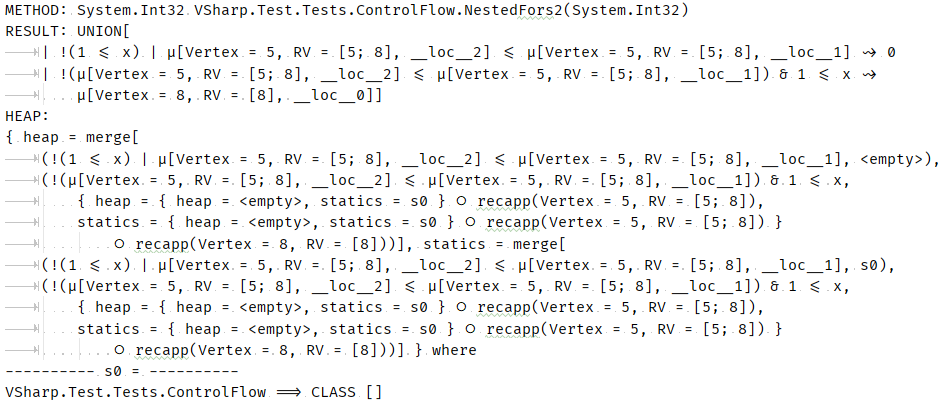
\includegraphics[scale=0.5]{Batoev/images/results.PNG}
\caption{Результат символьного исполнения метода~\ref{example:fors}}
\end{figure}

\begin{table}[t]
    \centering
    \begin{tabular}{ |p{3cm}||p{2cm}|p{2cm}|p{2cm}|  }
        \hline
        \multicolumn{4}{|c|}{Количественные характеристики тестов} \\
        \hline
        Название тестового набора &Количество тестов в наборе&Количество успешно пройденных тестов&Количество инструкций CIL\\
        \hline
        Arithmetics   &80    &77    &1968\\
        Logics        &75    &75    &1458\\
        Conditional   &10    &6     &943\\
        Recursive     &5     &5     &751\\
        Lambdas       &2     &2     &404\\
        Generic       &14    &14    &194\\
        Strings       &15    &15    &219\\
        Unsafe        &16    &16    &312\\
        Typecast      &19    &19    &969\\
        Methods       &10    &10    &238\\
        Lists         &9     &9     &1420\\
        Chess.NET     &1     &1     &2723\\
        \hline
        Всего         &256   &249   &11599\\
        \hline
    \end{tabular}
    \captionof{table}{Результаты тестирования}
    \label{experiments}
\end{table}


\FloatBarrier

\subsection{Тестирование интерпретатора}
Тестирование нового интерпретатора проводилось на тестовой подсистеме проекта <<VSharp.Test>> и на библиотеке \textsc{Chess.NET}.
Подсистема содержит тестовые наборы, затрагивающие различные конструкции и возможности языка C\#:
арифметику, логические операции,
работу с массивами разных размерностей, генерирование исключений, тесты на классы и структуры, включающие взаимодействие со статическими членами и вызовы виртуальных методов,
тесты с неограниченной рекурсией, тесты с \emph{unsafe}-кодом, тесты со строками. 

Таблица~\ref{experiments} показывает результаты проведенного тестирования. 
В наборах тестах с арифметикой и условными конструкциями была часть тестов с генерацией исключений. 
Поскольку схема обработки исключений для языка CIL не была реализована, то данные тесты были некорректно исполнены.
По той же причине не было проведено тестирования на тестовым наборе <<TryCatch>>, 
основное предназначение которого --- инициирование и перехват исключений.

\section{Заключение}

В данной работе описан подход к композициональному символьному исполнению без раскрутки. Была предложена концепция композициональной памяти с символьной адресацией. Был доказан некоторый набор свойств КСП, дающий основание для подхода в стиле систем переписывания, где символьные кучи могут сами выступать как символы. Это даёт возможность автоматически порождать уравнения на состояния, решения которых в точности отражают поведения функций, работающих с динамической памятью. Было показано как свести задачу решения уравнений на состояния к задаче проверки безопасности чистых функций второго порядка.

Данная работа нацелена на теоретические основания композиционального анализа динамической памяти. Мы оставляем апробацию этого подхода на будущее. Другим направлением будущих исследований может быть расширение нашего формализма на композициональный анализ параллельных программ.

\bibliographystyle{ugost2008ls}
\begin{thebibliography}{10}

\bibitem{baldoni2018survey}
Roberto Baldoni, Emilio Coppa, Daniele~Cono D’elia, Camil Demetrescu, and
  Irene Finocchi.
\newblock A survey of symbolic execution techniques.
\newblock {\em ACM Computing Surveys (CSUR)}, 51(3):50, 2018.

\bibitem{godefroid2007compositional}
Patrice Godefroid.
\newblock Compositional dynamic test generation.
\newblock In {\em ACM Sigplan Notices}, volume~42, pages 47--54. ACM, 2007.

\bibitem{jaffar2012tracer}
Joxan Jaffar, Vijayaraghavan Murali, Jorge~A Navas, and Andrew~E Santosa.
\newblock Tracer: A symbolic execution tool for verification.
\newblock In {\em International Conference on Computer Aided Verification},
  pages 758--766. Springer, 2012.

\bibitem{king1976symbolic}
James~C King.
\newblock Symbolic execution and program testing.
\newblock {\em Communications of the ACM}, 19(7):385--394, 1976.

\bibitem{kuznetsov2012efficient}
Volodymyr Kuznetsov, Johannes Kinder, Stefan Bucur, and George Candea.
\newblock Efficient state merging in symbolic execution.
\newblock {\em Acm Sigplan Notices}, 47(6):193--204, 2012.

\bibitem{mcmillan2010lazy}
Kenneth~L McMillan.
\newblock Lazy annotation for program testing and verification.
\newblock In {\em International Conference on Computer Aided Verification},
  pages 104--118. Springer, 2010.

\bibitem{kostyukov2018csewu}
Юрий~Олегович Костюков.
\newblock {\em Кучи как чистые функции:
  композициональное символьное исполнение
  без раскрутки}, pages 288--346.
\newblock 6. 2018.

\end{thebibliography}

\title{Композициональное символьное исполнение CIL-кода}

\titlerunning{Композициональное символьное исполнение CIL-кода}

\author{Батоев Константин Аланович}

\authorrunning{К.~А.~ Батоев}

\tocauthor{Константин Батоев}
\institute{St Petersburg State University\\
	\email{konstantin.batoev@gmail.com}}

\maketitle

% \renewcommand{\ttdefault}{cmtt}

\newsavebox\CBox
\newcommand\hcancel[2][0.1pt]{%
  \ifmmode\sbox\CBox{$#2$}\else\sbox\CBox{#2}\fi%
  \makebox[0pt][l]{\usebox\CBox}%
  \textcolor{red}{\rule[0.3\ht\CBox-#1/2]{\wd\CBox}{#1}}}

\captionsetup[figure]{name=Рисунок}

% \newtheorem*{proof}{Доказательство}

\renewcommand{\defnautorefname}{опр.}
\renewcommand{\lemautorefname}{лемм.}
\renewcommand{\remkautorefname}{зам.}
\renewcommand{\propautorefname}{св.}
\renewcommand{\exmpautorefname}{пр.}
\renewcommand{\thmautorefname}{теор.}
% \renewcommand{\crlrautorefname}{Corollary}
\renewcommand{\sectionautorefname}{разд.}
\newcommand{\algorithmautorefname}{лист.}
\newcommand{\algorithmcfname}{Листинг}
\makeatletter
\renewcommand{\ALG@name}{Листинг}
\makeatother

\algrenewcommand\alglinenumber[1]{\tiny #1:}

\lstdefinelanguage{Demo}
{
 morecomment = [l]{//}, 
 sensitive = true,
 morekeywords = {type, new, null,
   bool, int, write, read,
   fail, nop, let, alloc, in,
   if, then, else, call,
   true, false, and, or, not}
}

\definecolor{commentgreen}{RGB}{0,200,100}
\lstdefinestyle{demolang}{language=Demo,
    rulecolor=\color{blue!80!black},
    basicstyle=\ttfamily\footnotesize,
    keywordstyle=\color{blue}\ttfamily,
    stringstyle=\color{red}\ttfamily,
    commentstyle=\color{commentgreen}\ttfamily,
    numbers=left,
    numbersep=5pt,
    numberstyle=\tiny\color{black},
    escapechar=@,
    tabsize=2
}

\usemintedstyle{vs}

\counterwithin{lstlisting}{section}
\counterwithin{algocf}{section}

\fontfamily{times}
% \fontsize{10pt}{30pt}
\selectfont
\setlength{\parindent}{0em}
% \setlength{\parskip}{1em}
\renewcommand{\baselinestretch}{1.0}

\SetupFloatingEnvironment{listing}{name=Листинг}
\providecommand*{\listingautorefname}{лист.}
\renewcommand*{\figureautorefname}{рис.}
\renewcommand*{\tableautorefname}{табл.}
\SetAlgorithmName{Листинг}{лист.} 

\theoremstyle{plain}
\newtheorem{thm}{Теорема}%[section]
\newtheorem{lem}{Лемма}%[section]
% \newtheorem{crlr}{Corollary}%[section]

\theoremstyle{definition}
\newtheorem{defn}{Определение}
\newtheorem{remk}{Замечание}
\newtheorem*{remk*}{Замечание}
\newtheorem{prop}{Утверждение}
\newtheorem{exmp}{Пример}
% \newtheorem*{proof}{Доказательство}

% \newcommand{\defnautorefname}{опр.}
\newcommand{\lemautorefname}{лем.}
\newcommand{\remkautorefname}{зам.}
\newcommand{\propautorefname}{утв.}
\newcommand{\exmpautorefname}{пример}
\newcommand{\thmautorefname}{теор.}
% \renewcommand{\crlrautorefname}{Corollary}
\renewcommand{\sectionautorefname}{секция}
% \renewcommand{\algorithmautorefname}{Алгоритм}
% \renewcommand{\algorithmcfname}{Алгоритм}

% \renewcommand*{\Authsep}{\authorcr}
% \renewcommand*{\Authand}{\authorcr}
% \renewcommand*{\Authands}{\authorcr}

% \makeatletter
% \makeatother

\lstdefinelanguage{Demo}
{
 morecomment = [l]{//}, 
 sensitive = true,
 morekeywords = {new, null,
   fail, goto, halt,
   true, false, and, or, not}
}

\definecolor{commentgreen}{RGB}{0,200,100}
\lstdefinestyle{demolang}{language=Demo,
    rulecolor=\color{blue!80!black},
    basicstyle=\ttfamily\footnotesize,
    keywordstyle=\color{blue}\ttfamily,
    stringstyle=\color{red}\ttfamily,
    commentstyle=\color{commentgreen}\ttfamily,
    numbers=left,
    numbersep=5pt,
    numberstyle=\tiny\color{black},
    escapechar=@,
    tabsize=2
}

%%% For graph drawing
\definecolor {processblue}{cmyk}{0.96,0,0,0}
\definecolor {processgreen}{cmyk}{1,0,1,0}
\definecolor {processred}{cmyk}{0, 0.84, 0.80, 0.19}
\definecolor {processyellow}{cmyk}{0, 0, 1, 0}


%\newcommand{\csharp}[1]{\mintinline{csharp}{#1}}

\newcommand{\pex}{\textsc{Pex}}
\newcommand{\predator}{\textsc{Predator}}
\newcommand{\dotnet}{\textsc{.NET}}
\newcommand{\clang}{\textsc{C}}
\newcommand{\vsharp}{\textsc{V\#}}

\newcommand\addrset{loc}
\newcommand\termset{term}
\newcommand\guardset{guard}

\newcommand\eqby[1]{\mathrel{\stackrel{\mbox{\normalfont\tiny #1}}{=}}}
\newcommand\eqdef{\eqby{def}}

\newcommand\aite{ite}
\newcommand\ite[3]{\aite(#1,#2,#3)}
\newcommand\Ite[3]{\aite\big(#1,#2,#3\big)}
\newcommand\pair[2]{\langle#1, #2\rangle}
\newcommand\paiR[2]{\big\langle#1, #2\big\rangle}
\newcommand\mg[2]{#1=#2}
\newcommand\nmg[2]{#1\neq#2}
\newcommand\li[1]{LI(#1)}
\let\emptyheap\varepsilon
\newcommand\agrec{Rec}
\newcommand\agmerge{Merge}
\newcommand\agcompose{\bigcirc}
\newcommand\GRec[1]{\agrec\big(#1\big)}
\newcommand\GMerge[1]{\agmerge\big(#1\big)}
\newcommand\GCompose[2]{#1\agcompose#2}
\newcommand\agho{App}
\newcommand\gapp[1]{\agho(#1)}
\newcommand\GApp[1]{\agho\big(#1\big)}
\newcommand\aunion{\texttt{UNION}}
\newcommand\union[1]{\aunion\big(#1\big)}
\newcommand\Union[1]{\aunion\Big(#1\Big)}
\newcommand\aderef{readStore}
\newcommand\readTerm{readTerm}
\newcommand\writeTerm{writeTerm}
\newcommand\afind{find}
\newcommand\find[5]{\afind(#1,#2,#3,#4,#5)}
\newcommand\finD[5]{\afind\big(#1,#2,#3,#4,#5\big)}
\newcommand\Find[5]{\afind\Big(#1,#2,#3,#4,#5\Big)}
\newcommand\deref[2]{\aderef(#1,#2)}
\newcommand\Deref[2]{\aderef\big(#1,#2\big)}
\newcommand\compose[2]{#1\circ#2}
\newcommand\lmbd[2]{\lambda #1.#2}
\newcommand\lmbdx[1]{\lambda x.#1}
\newcommand\dom[1]{dom(#1)}
\newcommand\Dom[1]{dom\big(#1\big)}

\newcommand\Li[1]{LI\big(#1\big)}
\newcommand\amutate{writeStore}
\newcommand\amutateStack{writeStack}
\newcommand\mutate[3]{\amutate(#1,#2,#3)}
\newcommand\mutateStack[4]{\amutateStack(#1,#2,#3,#4)}
\newcommand\rdbodyext[6]{\Union{\big\{\paiR{#4\mg{#1}{#5}}{#6\big(#2(#5), xs\big)} \mid #5\in\dom{#2} \big\}\\&\qquad\qquad\qquad\cup\paiR{#4\bigwedge_{\mathclap{#5\in\dom{#2}}}{\nmg{#1}{#5}}}{#6\big(#3, xs\big)}}}
\newcommand\rdbody[4]{\rdbodyext{#1}{#2}{#3}{}{l}{#4}}
\newcommand\wrtbody[6]{\Union{&\paiR{\mg{#1}{#2}}{\writeTerm\big(#3,#4,#6\big)},
    \\&\paiR{\nmg{#1}{#2}}{\writeTerm\big(#5(#1),#4,#6\big)}}}
\newcommand{\var}[1]{\mathit{#1}}


\begin{abstract}
Известно, что наибольшую сложность в области верификации программ представляет задача доказательства корректности программ с циклическими участками кода. Опираясь на подход символьного исполнения программ и на введенные формализмы обобщённых куч в работе~\cite{kostyukov2018csewu}, данная работа представляет алгоритм композиционального символьного исполнения без раскрутки отношения перехода программ с произвольным графом потока управления. На его основе был реализован символьный интерпретатор языка CIL в проекте V\#, символьной виртуальной машине для анализа .NET. Была проведена апробация алгоритма на примерах, включающих сложные потоки управления, и интерпретатора на тестовой базе проекта VSharp.Test и на библиотеке Chess.NET.
\end{abstract}
\section*{Введение}
Поиск путей в графе с ограничением в виде формальных языков~\cite{FLCpathProblem} --- это задача, в которой формальные языки используются для задания множества искомых путей. В таком подходе каждый путь соответствует слову, состоящему из меток его рёбер, а ограничением на путь является принадлежность соответствующего ему слова некоторому заданному формальному языку.

В качестве класса формальных языков по иерархии Хомского наибольший интерес представляют контекстно-свободные языки. В отличие от регулярных они обладают большей выразительностью. Поэтому в задаче поиска путей контекстно-свободные ограничения позволяют задавать более сложные отношения между вершинами. Так, например, важный класс запросов поиска вершин, лежащих на одном уровне иерархии~\cite{zhlang-2016}, задаётся только контекстно-свободными, но не регулярными ограничениями. Запросы такого вида, как и другие запросы с контекстно-свободными ограничениями имеют широкое применение в биоинформатике~\cite{bio-application} и при обработке rdf-файлов~\cite{zhlang-2016}.

Наиболее удобным и подходящим инструментом для работы с граф\-структурированными данными являются графовые базы данных. Так же как и реляционные, графовые базы данных поддерживают свой язык запросов. С его помощью графовые базы данных позволяют решать вышеупомянутую задачу поиска путей. Но ограничения на пути, которые поддерживается в наиболее распространённых базах данных, являются в лучшем случае регулярными.

Отсутствие поддержки контекстно-свободных ограничений в графовых базах данных, во-первых, сильно ограничивает выразительность языка запросов. Во-вторых, при необходимости в более сложных запросах разработчикам приходится самим писать алгоритмы, решающие задачу контекстно-свободной достижимости для их частного случая. Так, например, Хуэй Мяо и др.~\cite{datascince-lifecycle} разработали систему хранения и отслеживания версий артефактов, возникающих при научных работах. Вся информация про артефакты хранилась в графовой базе данных. При этом при разработке возникла потребность в выполнении запросов с контекстно-свободными ограничениями для выявления взаимоотношений между различными версиями различных артефактов. Это и послужило началом статьи~\cite{datascince-lifecycle}, в которой приводятся алгоритмы решения частных запросов.

В недавнем исследовании Йохем Куйперс и др.~\cite{Kuijpers:2019:ESC:3335783.3335791} произвели сравнительный анализ наиболее известных алгоритмов поиска путей с конте\-кстно-свободными ограничениями. Алгоритмы запускались на графах, находящихся в хранилище графовой базы данных Neo4j. По результатам исследования было показано, что в контексте Neo4j алгоритмы обладают большим временем работы, и поэтому дальнейшая работа по расширению языка запросов прекратилась. При этом Рустам Азимов~\cite{Azimov:2018:CPQ:3210259.3210264} предоставил матричный алгоритм и его реализацию, которая работает за разумное время на реальных данных. Но, так как алгоритм был реализован вне контекста базы данных, его результат приняли недостаточно показательным. Поэтому вопрос о реализуемости запросов с контекстно-свободными ограничениями в графовых базах данных, а соответственно и о возможности расширения языка запросов для их поддержки остаётся открытым.

\section{Постановка задачи}
Целью данной работы является полная поддержка запросов с конте\-кстно-свободными ограничениями для графовой базы данных. А именно, необходимо предоставить пользователю возможность формулировать запросы с контекстно-свободными ограничениями в терминах одного из существующих стандартных языков запросов и исполнять их в графовой базе данных за приемлемое время. Для достижения этой цели были поставлены следующие задачи.

\begin{itemize}
    \item Выполнить обзор существующих реализаций поддержки запросов с контекстно-свободными ограничениями в графовых базах данных. В результате обзора необходимо выбрать наиболее перспективный с точки зрения производительности алгоритм решения задачи контекстно-свободной достижимости и подходящую для его интеграции базу данных. При выборе базы данных необходимо учитывать как возможность интеграции выбранного алгоритма, так и возможность поддержки одного из стандартных языков запросов, позволяющего выражать контекстно-свободные ограничения.
    \item Интегрировать выбранный на предыдущем шаге алгоритм в выбранную графовую базу данных.
    \item Расширить язык запросов выбранной базы данных конструкциями, необходимыми для выражения контекстно-свободных ограничений.
    \item Произвести замеры производительности полученного решения и сравнить его с существующими решениями.
\end{itemize}


\section{Обзор}

\subsection{Терминология}
Контекстно-свободной грамматикой называется $G = (\Sigma, N, P, S)$, где $\Sigma$ --- алфавит терминальных символов, $N$ --- алфавит нетерминальных символов, $P$ --- множество правил вида $A \rightarrow \alpha$, где $A \in N$, $\alpha \in (\Sigma \cup N)^*$, а $S \in N$ --- выделенный стартовый нетерминал.

% \gsv{про S забыли}.

Языком $L$ над алфавитом $\Sigma$ называется любое подмножество $2^{\Sigma^*}$. Языком, порождаемой грамматикой G, является множество $L(G) = \{S \xRightarrow{*} \beta, \beta \in \Sigma^*\}$, где $S \xRightarrow{*} \beta$ означает, что из нетереминала $S$ путём последовательного применения правил грамматики выводится $\beta$.

Контекстно-свободная грамматика $G = (\Sigma, N, P, S)$ находится в осла\-бленной нормальной форме Хомского, если любое её правило имеет вид $A \rightarrow BC$, где $A, B, C \in N$, либо $A \rightarrow a$, где $A \in N, a \in \Sigma$. В отличие от нормальной формы Хомского в ослабленной, во-первых, допускается присутствие стартового нетерминала $S$ в правых частях правил грамматики, во-вторых, запрещаются правила вида $S \rightarrow \epsilon$, где $\epsilon$ --- пустая строка.

% \gsv{Это не нормальная форма Хомского. У НФХ есть дополнительные ограничения. Мы называем то, что здесь, ослабленной НФХ. Важно отдельно проговорить разницу с НФХ.}

В задаче поиска путей с ограничениями в виде формальных языков дан граф $(V, E)$, разметка его рёбер $l: E \rightarrow \Sigma$ и язык $L$ над алфавитом $\Sigma$. Требуется найти множество всех пар вершин, между которыми существует путь, метки на рёбрах которого образуют слово в заданном языке. То есть требуется найти следующее множество:
\[\{(v, to): \exists p=(e_1,...,e_n) \in E^*: l(e_1)...l(e_n) \in L,~src(e_1)=v,~dst(e_n)=to\}\]
Здесь $src(e)$ и $dst(e)$ для $e \in E$ означают начальную и конечную вершину ребра $e$. В данном контексте язык $L$ называется языком ограничений.
% \gsv{У Вас вершины v и to никак с путём не связаны}

Задача поиска путей с контекстно-свободными ограничениями --- это задача поиска путей в виде формальных языков, в которой язык задаётся контекстно-свободной грамматикой.

\subsection{Графовые базы данных}
Графовые СУБД\footnote{СУБД --- Система управления базами данных} (далее просто графовые базы данных) --- это разновидность СУБД, в которой данные хранятся в виде графов. В отличие от других разновидностей, в графовых базах данных отношения между объектами так же важны, как и сами объекты.

Основной моделью представления графов в таких базах данных является gpraph property model~\cite{graph-propery-model}. В ней каждая сущность может содержать набор свойств в формате ключ-значение. Основными сущностями являются узлы и отношения. Узлы соответствуют вершинам графа и помимо свойств могут иметь несколько меток. Отношения соответствуют рёбрам и имеют ровно одну метку, которая называется типом отношения. На рисунке~\ref{fig:graph_bd_1} показан небольшой пример графа в такой модели. 

\begin{figure}[h]
\centering
    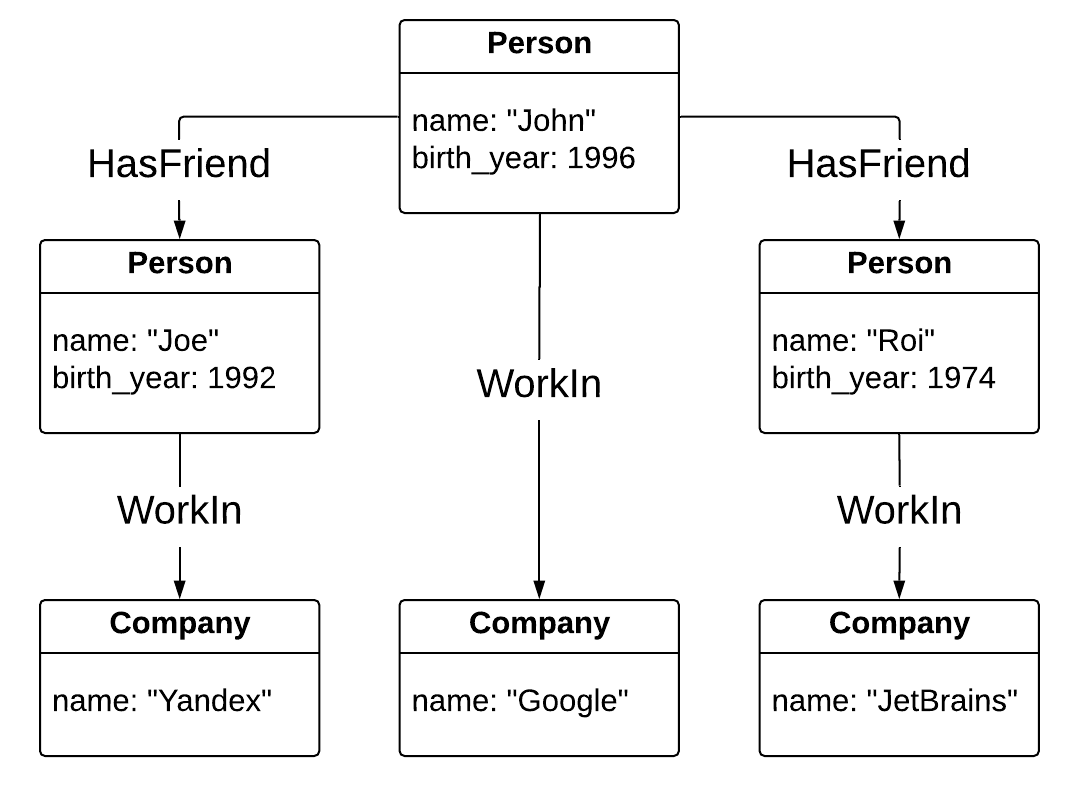
\includegraphics[width=0.7\linewidth]{Terekhov/pictures/graph_bd_1.png}
    \caption{Пример социального графа}
    \label{fig:graph_bd_1}
\end{figure}

Для работы с графами графовые базы данных предоставляют язык запросов, самым популярным из которых является Cypher~\cite{cypher-language}. В нём главный интерес представляют запросы вида сопоставления с образцом. Они позволяют задавать интересующие пути или подграфы в виде шаблонов и описывать информацию, которую нужно извлечь после удачного сопоставления. На рисунке~\ref{code:cypher_query} приведён пример такого запроса. Шаблон пути описывается в выражении MATCH. В нём между круглыми скобками задаются шаблоны вершин, а между квадратными шаблоны рёбер. Таким образом в данном примере задаются следующие ограничения: путь должен начинаться из вершины с меткой Person и именем John и состоять из двух рёбер, первое из которых должно иметь тип HasFriend, а второе WorkIn. В выражении RETURN задаётся информация, которую нужно извлечь. В данном примере это имя последней в пути вершины. В итоге ответом на такой запрос являются имена компаний, в которых работают друзья Джона. Результатом работы этого запроса на графе из рисунка~\ref{fig:graph_bd_1} является множество \{"Yandex", "JetBrains"\}.

%\lstset{
%   basicstyle=\fontsize{14}{14}\selectfont\ttfamily
%}

\begin{figure}[h]
\begin{lstlisting}[language=sql]
MATCH (p:Person)-[:HasFriend]->()-[:WorkIn]->(to)
WHERE p.name = "John"
RETURN to.name
\end{lstlisting}
\caption{Пример конечного запроса на языке Cypher}
\label{code:cypher_query}
\end{figure}

С формальной точки зрения шаблоны пути в выражении MATCH позволяют поставить задачу поиска путей с ограничениями в виде формальных языков. Так в запросе на рисунке~\ref{code:cypher_query} языком ограничений является конечный язык $\{(HasFriend, WorkIn)\}$. Для запроса на рисунке~\ref{code:cypher_query_2} ограничением является регулярный язык $\{A, B\}^*$. 

\begin{figure}[h]
\begin{lstlisting}[language=sql]
MATCH (v)-[:A | :B *]->(to)
RETURN to.name
\end{lstlisting}
\caption{Пример регулярного запроса на языке Cypher}
\label{code:cypher_query_2}
\end{figure}

При этом регулярные ограничения поддерживаются лишь частично и позволяют искать только пути произвольной длины с заданными метками на рёбрах, а более глубокие регулярные выражения не поддерживаются. Поэтому на текущий момент язык запросов довольно ограничен.

\subsection{Существующие решения}
Как было упомянуто раннее, ни одна графовая база данных не поддерживает запросов с контекстно-свободными ограничениями. Тем не менее существуют альтернативные решения поддержки таких запросов. 

\subsubsection{Парсер-комбинаторы для Neo4j}\label{sec:pareser-combinators}
В 2018 году группой исследователей из JetBrains Research на основе библиотеки Meerkat была разработана библиотека для поддержки запросов с контекстно-свободными ограничениями~\cite{parser-combinators}. Она использует графовую базу данных Neo4j~\cite{neo4j} как хранилище графов и позволяет задавать запросы в виде парсер-комбинаторов. Основным достоинством данной работы является то, что с помощью этой библиотеки кроме контекстно-свободных запросов можно выразить базовую часть языка Cypher. Но так как конкурировать с оригинальной реализацией выполнения запросов Neo4j очень сложно, это достигается вместе c сильной потерей производительности. Кроме этого контекстно-свободные запросы обрабатываются также достаточно медленно.

Таким образом данное решение является альтернативой языка запросов Neo4j, а не его расширением. Из-за медленного времени работы такое решение подходит только для работы с небольшими графами. 

\subsubsection{Расширение языка запросов SPARQL}\label{subsection:cypher-extention-2}
%Про sparql%
В 2016 Сяованг Чжан предоставил язык cfSPARQL~\cite{zhlang-2016} --- расширение языка SPARQL, который способен выразить запросы с контекстно-свободными ограничениями. Также он привёл алгоритм для вычисления таких запросов и замеры производительности. Но, во-первых, работа была сделана вне контекста графовой базы данных, а во-вторых, время работы предложенного алгоритма было больше, чем время работы парсер-комбинаторов.

\subsubsection{Существующие реализации алгоритмов решения задачи контекстно-свободной достижимости}
Основной сложностью расширения языка запросов для поддержки запросов с контекстно-свободными ограничениями является долгое время работы соответствующих алгоритмов. Так, например, в 2019 году Йохем Куйперс и другие исследователи с целью попытки расширения языка запросов Cypher для графовой базы данных Neo4j произвели сравнительный анализ производительности наиболее известных алгоритмов решения задачи контекстно-свободной достижимости.

В данном исследовании были рассмотрены и произведены замеры времени работы алгоритма Элле Хелингса~\cite{hellings-2015}, основанного на атрибутных грамматиках, восходящего алгоритма Фреда Сантоса~\cite{santos-2018}, матричного алгоритма Рустама Азимова~\cite{Azimov:2018:CPQ:3210259.3210264} и алгоритма Петтери Севона~\cite{bio-application}. Все алгоритмы были интегрированы в Neo4j и запускались на графах, находящихся в её хранилище. Алгоритмы были написаны на языке Java, при этом их реализация являлась однопоточной.

% \gsv{В таких местах надо сразу ссылку на алгоритм давать.}

По результатам замеров производительности было показано, что время работы алгоритмов является слишком большим и неприемлемым для широкого практического использования. Поэтому дальнейшая работа по интеграции и расширению языка запросов была приостановлена.

Тем не менее, матричный алгоритм Рустама Азимова в сравнительном анализе Йохема Куйперса был реализован без необходимых матричных библиотек, которые могут сильно уменьшить время его работы. Так, например, в исследовании Никиты Мишина и др.~\cite{azimov-evalution} был произведён сравнительный анализ времени работы нескольких реализаций алгоритма Рустама Азимова, основанных на различных специализированных матричных библиотеках. Графы и запросы к ним были взяты из объемлющего набора данных CFPQ\_Data~\cite{cfpq-data}, предоставленного лабораторией языковых инструментов JetBrains Research. 

Результаты замеров Никиты Мишина и др. показали, что при грамотной реализации алгоритма Рустама Азимова и использовании подходящих матричных библиотек можно добиться очень высокой производительности. Поэтому, так как основной проблемой применимости запросов с контекстно-свободными ограничениями является долгое время работы соответствующих алгоритмов, в качестве алгоритма решения задачи конте\-кстно-свободной достижимости был выбран матричный алгоритм Рустама Азимова.

\subsection{Матричный алгоритм Рустама Азимова}\label{sec:matrix-algo}
Выбранный в предыдущей главе алгоритм Рустама Азимова~\cite{Azimov:2018:CPQ:3210259.3210264}, в отличие от других алгоритмов решения задачи контекстно-свободной достижимости~\cite{hellings-2015, santos-2018, zhlang-2016}, работает с графами в виде разреженных матриц смежности. Данный алгоритм состоит из последовательности операций над разреженными матрицами, время работы которых зависит не от размеров матричных операндов, а от количества их ненулевых элементов.

На вход алгоритму (см. алгоритм 1) поступает помеченный граф $D=(V,E)$ и контекстно-свободная грамматика $G=(\Sigma, N, P, S)$ в ослабленной нормальной форме Хомского. Для каждого нетерминала $A$ в ассоциативном массиве $T$ хранится соответствующая ему булева матрица $T[A]$. На всём этапе алгоритма поддерживается следующий инвариант: $T[A]_{i,j} = 1$ равносильно существует пути, метки на рёбрах которого образуют слово, выводящееся из нетерминала $A$. На первом этапе происходит инициализация матриц с помощью простых правил грамматики, после чего инвариант выполняется для всех путей единичной длины. На втором этапе происходит транзитивное замыкание, после чего этот инвариант верен для всех путей. Результатом данного алгоритма является матрица, соответствующая стартовому нетерминалу $S$.

%  Это позволяет для его реализации использовать многопоточные матричные библиотеки, с помощью которых можно добиться очень высокой производительности. Поэтому на текущий момент алгоритм Рустама Азимова показывает наилучшее время работы на практике.

\begin{algorithm}
\caption{Матричный алгоритм Рустама Азимова}

\begin{algorithmic}[1]
\Function{contextFreePathQuerying}{$D$, $G$}
    \State{$n =$ getNodeCount(D)}
    \State{$N =$ getAllNonterms(G)}
    \State{$E =$ getEdges($D$)}
    \State{$P =$ getRules($G$)}
    \State{$S =$ getStartNonterm($G$)}
    \State{$T = \{A \rightarrow \varnothing_{n \times n} : A \in$ $N$ \} }
    \ForAll{$(v, to, label) \in E$}
    \Comment{Инициализация матриц}
        \ForAll{$A \rightarrow label \in P$}
            \State{$T[A]_{i,j} = 1$}
        \EndFor
    \EndFor    
    \While{$\exists A: T[A]$ is changing}
    \Comment{Вычисление замыкания}
        \ForAll{$A \rightarrow BC \in P$}
            \State{$T[A] \oplus= T[B] \otimes T[C]$}
        \EndFor
    \EndWhile
\State \Return $T[S]$
\EndFunction

\end{algorithmic}
\end{algorithm}

Практическое время работы алгоритма Рустама Азимова сильно зависит от производительности используемой матричной библиотеки. Это накладывает некоторые ограничения на выбор подходящей графовой базы данных, так же как и возможность представления графов в матричном виде.

\subsection{RedisGraph}
RedisGraph~\cite{redis-graph} --- это высокопроизводительная графовая база данных, поддерживающая язык запросов Cypher. В отличие от наиболее распространённой графовой базы данных Neo4j~\cite{neo4j}, RedisGraph написан на языке Си и для работы с данными использует Redis~\cite{redis}, основным достоинством которого является возможность хранить данные прямо в оперативной памяти. Это позволяет RedisGraph быстро обрабатывать пользовательские запросы.

Также RedisGraph является единственной графовой базой данных, которая работает с графами в виде разреженных матриц смежности и транслирует запросы языка Cypher в матричные выражения. Для представления графов в таком виде и работы с ними в терминах линейной алгебры используется мощный матричный фреймворк GraphBlas~\cite{graph-blas}. Его реализация SuiteSparse~\cite{suite-sparse} является многопоточной и сильно оптимизирована, что позволяет RedisGraph добиться высокой производительности.

Из всего этого следует, что RedisGraph идеально подходит для интеграции матричного алгоритма. Во-первых, графы представляются в необходимом алгоритму виде, что позволит избежать издержек на конвертацию форматов. Во-вторых, использование SuiteSparse для вычисления матричных операций позволит добиться высокой производительности. Поэтому RedisGraph был выбран в качестве графовой базы данных для интеграции матричного алгоритма и расширения языка запросов.

% Так как алгоритм Рустама Азимова работает с матричным представлением графа,, как наиболее подходящий для интеграции матричного алгоритма.

\subsection{Расширение языка Cypher}\label{subsection:cypher-extention}
На текущий момент оригинальная версия языка Cypher, используемая в том числе и в RedisGraph, не поддерживает запросов с контекстно-свободными ограничениями. Но тем не менее в 2017 году был разработан черновой вариант спецификации расширения Cypher~\cite{cypher-specification}, которая вводит в язык шаблоны путей. Они позволяют выразить более сложные запросы, в том числе запросы с контекстно-свободными ограничениями.

Шаблоны путей являются альтернативой шаблонам рёбер, которые есть в оригинальном Cypher. Они, как и шаблоны рёбер, могут встречаться в выражении MATCH и иметь своё направление. Кроме этого в глобальной области запроса им можно задавать имя, на которое потом можно ссылаться внутри других шаблонов.

Шаблон пути представляет из себя регулярное выражение над некоторыми примитивами. В качестве таких примитивов могут выступать шаблоны рёбер, шаблоны вершин и ссылки на именованные шаблоны путей. Также любым подвыражениям можно задавать своё направление. Основная часть конкретного синтаксиса данного расширения приведена на рисунке~\ref{fig:cypher_syntax}.

\begin{figure}[]
\begin{align*}
\begin{split}
PathPattern     &= ["<"],~"-/",~PathExpression,~"/-",~[">"]\\
PathExpression  &= \{PathAlternative\}\\
PathAlternative &= PathRepetition,~\{"|", PathRepetition\}\\
PathRepetition  &= ["<"],~PathBase,~[">"],~("*")
\end{split}\\
\begin{split}
PathBase &= PathEdge \\
         &~~|~PathNode \\
         &~~|~PathReference \\
         &~~|~"[",~PathExpression,~"]"
\end{split}\\
\begin{split}
PathEdge      &= Label \\
PathNode      &= "(",~[Label,~\{"|",~Label\}],~")" \\
PathReference &= "\sim",~SymbolicName; \\
Label         &= ":",~LabelName
\end{split}
\end{align*}
\caption{Расширение конкретного синтаксиса Cypher}
\label{fig:cypher_syntax}
\end{figure}

Каждый шаблон пути задаёт отношение на множестве вершин. Поэтому семантикой языка шаблонов путей $L_{P}$ в контексте графа $G(V, E)$ является отображение $\llbracket \cdot \rrbracket_{G}: L_P \rightarrow V \times V$, которое каждому шаблону $p\in L_P$ сопоставляет множество пар вершин, между которыми существует путь, удовлетворяющий данному шаблону $p$. 

Подробное описание данной семантики приводится в таблице~\ref{tab:cypher_sematic}.  В ней наибольший интерес представляют именованные шаблоны путей, так как именно с помощью них можно выразить запросы с контекстно-свободными ограничениями. Все именованные шаблоны путей $S_i = p_j$ можно рассматривать как правила контекстно свободной грамматики с алфавитом нетерминалов $\{S_i\}_{i=1}^n$. Тогда каждый нетерминал $S_j$ порождает язык $L_{S_j} \subset L_p$, а семантикой соответствующего именованного шаблона пути $S_j=p_j$ является множество $\bigcup\limits_{p \in L_{s_j}} \llbracket p \rrbracket_{G}$.

На рисунке~\ref{code:cypher_query_3} приведён пример запроса в расширенном синтаксисе. В нём декларируется именованный шаблон S, который задаёт множество правильных скобочных последовательностей над ребрами с типом L и R. Далее в выражении MATCH задаётся шаблон пути, состоящий из ссылки на шаблон S. Таким образом результатом обработки запроса является множество всех пар вершин, между которыми существует путь, метки на рёбрах которого образуют правильную скобочную последовательность. 

\begin{table}[h!]
\begin{adjustbox}{max width=\textwidth}
\begin{tabular}{|c|c|c|}
\hline
$p \in L_P$                                                                                  & $\llbracket p \rrbracket_{G}$                                                                                                                                                                                   & Описание шаблона пути                                                                                                         \\ \hline
\hline
()                                                                                            & $\{(v, v): v \in V\}$                                                                                                                                                                                           & \begin{tabular}[c]{@{}c@{}}Пустой путь, состоящий из \\ одной произвольной вершины\end{tabular}                               \\ \hline
:a                                                                                            & $\{e=(v,to): e \in E, type(e)=a\}$                                                                                                                                                                              & \begin{tabular}[c]{@{}c@{}}Путь единичной длины,\\  состоящий из ребра с типом $a$\end{tabular}                               \\ \hline
(:b)                                                                                          & $\{(v, v): v \in V, label(v)=b\}$                                                                                                                                                                               & \begin{tabular}[c]{@{}c@{}}Пустой путь, состоящий из одной\\  вершины, помеченной меткой $b$\end{tabular}                     \\ \hline
$\alpha~\beta$                                                                                & $\llbracket \alpha \rrbracket_{G}\circ \llbracket \beta \rrbracket_{G}$                                                                                                                                         & Конкатенация путей $\alpha$ и $\beta$                                                                                         \\ \hline
$\alpha~|~\beta$                                                                              & $\llbracket \alpha \rrbracket_{G}\cup \llbracket \beta \rrbracket_{G}$                                                                                                                                          & Альтренатива между путями $\alpha$ и $\beta$                                                                                  \\ \hline
$[\alpha]$                                                                                    & $\llbracket \alpha \rrbracket_{G}$                                                                                                                                                                              & \begin{tabular}[c]{@{}c@{}}Квадратные скобки позволяют \\ группировать  выражения \\ для задания ассоциативности\end{tabular} \\ \hline
\textless{}$\alpha$                                                                           & $\{(to, v): (v, to) \in \llbracket \alpha \rrbracket_{G}\}$                                                                                                                                                     & Путь, обратный к пути $\alpha$                                                                                                \\ \hline
\textless{}$\alpha$\textgreater{}                                                             & $\llbracket \alpha~|~$\textless{}$\alpha \rrbracket_{G} $                                                                                                                                                       & \begin{tabular}[c]{@{}c@{}}Альтернатива между путём $\alpha$ и\\ обратным к нему\end{tabular}                                 \\ \hline
$\alpha^*$                                                                                    & $\llbracket \alpha \rrbracket_{G}^{*}$                                                                                                                                                                          & \begin{tabular}[c]{@{}c@{}}Путь, состоящий из\\ конкатенации 0 или более путей $\alpha$\end{tabular}                          \\ \hline
\begin{tabular}[c]{@{}c@{}}$\{S_i = p_i\}_{i=1}^{n}$\\ -- named\\  path patterns\end{tabular} & \begin{tabular}[c]{@{}c@{}}$P = \{S_i \rightarrow p_i\}_{i=1}^n$\\ $Gram_j = (\Sigma, \{S_i\}_{i=1}^n, P, S_j)$\\ $\llbracket S_j \rrbracket_{G} = \bigcup\limits_{p \in L(G)}{\llbracket p \rrbracket_{G}}$\end{tabular} & Именнованые шалоны путей                                                                                                      \\ \hline
$\sim$$S$                                                                                     & $\llbracket S \rrbracket_{G}$                                                                                                                                                                                   & \begin{tabular}[c]{@{}c@{}}Ссылка на именнованный\\  шаблон пути\end{tabular}                                                 \\ \hline
\end{tabular}
\end{adjustbox}
\caption{Семантика языка шаблонов путей}
\label{tab:cypher_sematic}
\end{table}

\begin{figure}[h!]
\begin{lstlisting}[language=sql]
PATH PATTERN S = ()-/ [:L ~S :R] | [~S ~S] | () /-()
MATCH (v)-/ ~S /-(to)
RETURN v, to
\end{lstlisting}
\caption{Пример запроса в расширенном синтаксисе Cypher}
\label{code:cypher_query_3}
\end{figure}

Данная спецификация расширения Cypher была представлена официальными разработчиками и сильно расширяет выразительность языка, предоставляя удобную возможность выражать запросы как с регулярными, так и с контекстно-свободными ограничениями. Поэтому в моей работе приводится поддержка выполнения запросов именно для этого расширения языка.

% \gsv{Не хватает какого-то чёткого вывода про то, что вот именно это мы и буем использовать.}

\section{Реализация}
По результатам обзора было решено реализовать поддержку расширения языка Cypher, представленную в главе~\ref{subsection:cypher-extention}, для графовой базы данных RedisGraph. За основу алгоритма, решающего задачу поиска путей с контекстно-свободными ограничениями, был взят матричный алгоритм Рустама Азимова, описанный в главе~\ref{sec:matrix-algo}.

% \gsv{И зжесь надо ещё раз подитожить в духе "по результатм обзора было решено сделать то и это с использованием того и сего"}

\subsection{План выполнения запроса}\label{execution-plan}
В RedisGraph основной частью обработки запроса является построение плана его выполнения. Её часть, которая относится к шаблонам путей приведена на рисунке~\ref{fig:execution_plan}. В ней зелёным цветом выделено то, что было добавлено или расширено.

В самом начале, после получения запроса строится его абстрактное синтаксическое дерево \textit{AST}. Далее, из него извлекаются именованные и неименованные шаблоны путей \textit{PathPattern} и \textit{NamedPathPatterns}, после чего они преобразуются в более удобное промежуточное представление \textit{PathExpr}. При этом, для дальнейшего связывания ссылок, именованные шаблоны сохраняются в глобальном контексте запроса \textit{PathPatternCtx}.

На следующем этапе происходит трансляция промежуточных представлений \textit{PathExpr} в матричные выражения \textit{AlgebraicExpression}. В них операндами являются либо матрицы, полученные из указанного в запросе графа \textit{GraphCtx}, либо ссылки на именованные шаблоны путей из \textit{PathPatternCtx}. Основной идеей трансляции является то, что после вычисления матричного выражения получается матрица, которая задаёт то же самое отношение на множестве вершин, что и исходный шаблон пути.

Далее каждое такое выражение формирует новую операцию плана выполнения запроса \textit{CfpqTraverseOp}. При её вычислении сначала происходит запуск расширенной версии матричного алгоритма Рустама Азимова. Он решает задачу контекстно-свободной достижимости, заданной именованными шаблонами путей. После этого все ссылки в матричном выражении заменяются на полученные в ходе алгоритма матрицы и происходит вычисление матричного выражения. Каждая такая операция добавляется в план выполнения запроса.

%  \gsv{Используйте \textit{CfpqTraverseOp} вместо долларов для длинных слов. Они тогда не распадаются из-а лишних пробелов.}

\begin{figure}[H]
\centering
    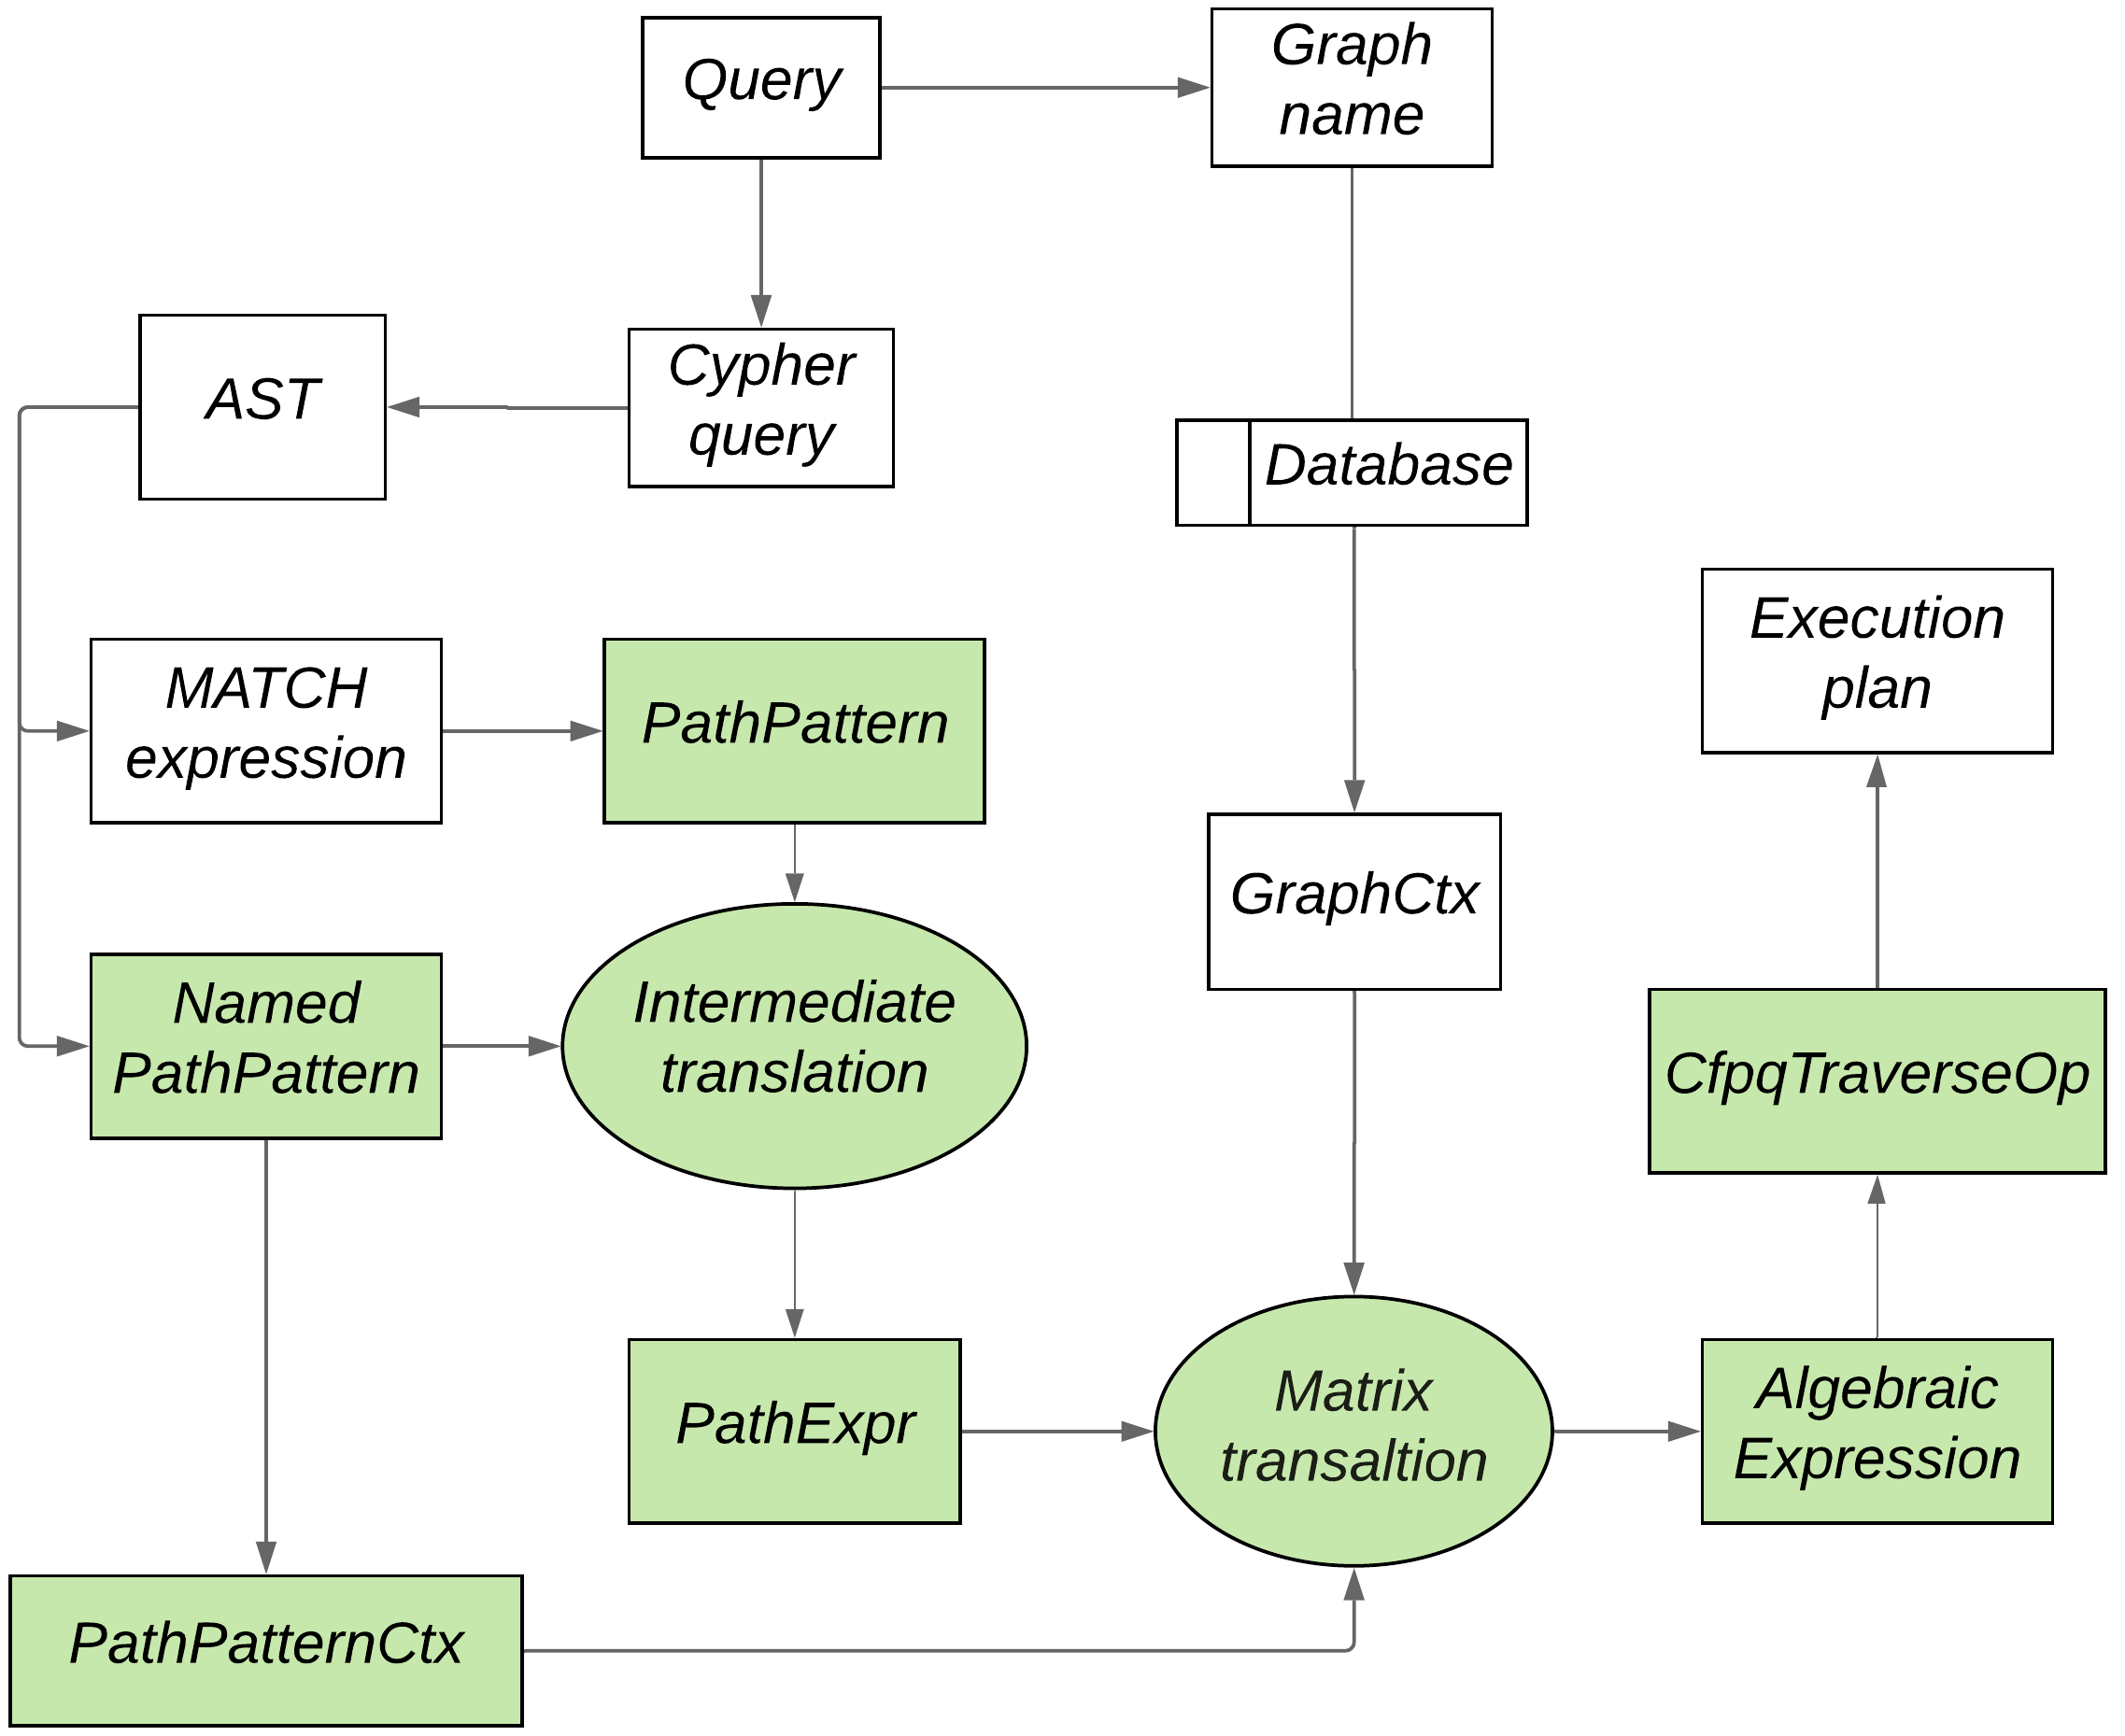
\includegraphics[width=1.0\linewidth]{Terekhov/pictures/execution_plan_3.png}
    \caption{Расширение построения плана выполнения запроса}
    \label{fig:execution_plan}
\end{figure}

\subsection{Промежуточное представление}\label{matrix-translation}
Шаблоны путей, полученные из \textit{AST}, транслируются в промежуточное представление \textit{PathExpr}. Оно позволяет задавать более простой абстрактный синтаксис, который описан на рисунке~\ref{fig:intermidiate_repr}. 

Таким образом, альтернативе и конкатенации шаблонов соответствуют \textit{PathAlt} и \textit{PathSeq}, \textit{PathGroup} позволяет задавать направление пути и наличие замыкания, а \textit{PathBasic} соответствует либо примитивным шаблонам \textit{PathNode}, \textit{PathEdge} и \textit{PathRef}, либо целому выражению \textit{PathExpr}. Примеры промежуточного представления шаблонов приведены в таблице~\ref{tab:inter_examples}.
\begin{figure}[h!]
\begin{align*}
\begin{split}
PathExpr=~ &PathSeq(PathExpr,~PathExpr)~|\\
           &PathAlt(PathExpr,~PathExpr)~|\\
           &PathGroup(PathBasic, direction, range)
\end{split}\\
\begin{split}
PathBasic=~ &PathNode(label)~|\\
            &PathEdge(type)~~|\\
            &PathRef(name) ~~|\\
            &PathExpr
\end{split}\\
\begin{split}
direction \in ~&\{inbound,~outbound,~bidirectional\}\\
range \in     ~&\{*, \varnothing\}
\end{split}
\end{align*}
\caption{Промежуточное представление PathExpr}
\label{fig:intermidiate_repr}
\end{figure}

\begin{table}[h]
\centering
\begin{adjustbox}{max width=\textwidth}
\begin{tabular}{|c|l|}
\hline
$L_p$                        & \multicolumn{1}{c|}{PathExpr}                                                                                                        \\ \hline
{[}:A :B{]} | (:C)           & \begin{tabular}[c]{@{}l@{}}$PathAlt($\\ $~~~~PathSeq(PathEdge("A"),~PathEdge("B"))$\\ $~~~~PathNode("C")$\\ $)$\end{tabular}         \\ \hline
\textless{}{[}:A $\sim$S{]}* & \begin{tabular}[c]{@{}l@{}}$PathGroup($\\ $~~~~PathSeq(PathEdge("A"),~PathRef("S")),$\\ $~~~~inbound,$\\ $~~~~*,$\\ $)$\end{tabular} \\ \hline
\end{tabular}
\end{adjustbox}
\caption{Примеры промежуточного представления запросов}
\label{tab:inter_examples}
\end{table}

\newpage
\subsection{Трансляция в матричные выражения}
Как было упомянуто ранее, RedisGraph представляет графы в виде разреженных матриц. А именно каждый граф $G$ задаётся следующей тройкой $(A \in M_{n\times n},~lab \in Labels \rightarrow Diag_n,~rel \in RelTypes \rightarrow M_{n \times n})_G$. Здесь $M_{n \times n}$ означает полукольцо булевых матриц, а $Diag_n$ полукольцо диагональных булевых матриц. Матрица $A$ служит матрицей смежности графа, а отображения $lab$ и $rel$ сопоставляют меткам вершин и типам рёбер соответствующие булевы матрицы. Таким образом, ребро $(v, to)$ графа $G$ имеет тип $a$ тогда и только тогда, когда $rel(a)_{v,to} = 1$.  Таким же образом, принадлежность метки $l$ вершине $v$ равносильно $lab(l)_{v,v}=1$.

Любую булеву матрицу $M$, участвующую в задании графа $G(V, E)$, можно рассматривать как отношение на множестве вершин $R(M) = \{(v, to):~M_{v,to}=1\}$. Операциями сложения и умножения в булевом полукольце являются дизъюнкция и конъюнкция. Поэтому умножению матриц $A*B$ соответствует композиция отношений $R(A) \circ R(B)$, сложению $A+B$ соответствует объединение отношений $R(A) \cup R(B)$, а транспонированная матрица $A^T$ соответствует обратному к R(A) отношению $R(A)^{-1}$. Такая взаимосвязь между матричными операциями и отношениями лежит в основе алгоритма трансляции, приведённом на рисунке~\ref{algo:translation}.

Данный алгоритм является рекурсивным и принимает на вход промежуточное представление шаблона пути $expr$, представление графа $g$ и контекст именованных шаблонов путей $pathCtx$. Целевым языком трансляции является простой язык матричных выражений, приведённый на рисунке~\ref{fig:alg-expr}.

Базовым случаем рекурсии являются примитивные шаблоны \textit{Path\-Node}, \textit{PathEdge} и \textit{PathReference}, которые транслируются в операнды матричного выражения. Для первых двух соответствующие матрицы извлекаются из графа с помощью функций \textit{GetLabel\-Matrix} и \textit{GetRelation\-Matrix}. При этом случай $label = \varnothing$ соответствует шаблону пути, состоящему из одной произвольной вершины. Поэтому такой путь задаётся тождественным отношением $R(I)$, где $I$ --- единичная матрица. Для \textit{Path\-Reference} создаётся ссылка на матрицу именованного шаблона, которая будет вычислена на следующем этапе при выполнении алгоритма контекстно-свободной достижимости.

Трансляция для шаблонов \textit{PathSeq} и \textit{PathAlt} происходит одинаковым образом --- сначала происходит трансляция дочерних шаблонов, а потом из полученного результата образуются операции умножения или сложения. Такая трансляция обосновывается семантикой шаблонов альтернативы и конкатенации, приведенной в главе~\ref{subsection:cypher-extention}, и связью отношений с матричными операциями, описанными раннее.

Наиболее интересным случаем является трансляция \textit{Path\-Group}, так как в некоторых случаях контекст именованных шаблонов $pathCtx$ расширяется. В начале происходит трансляция дочернего шаблона. Далее, если заданное направление является обратным, к полученной матрице применяется операция транспонирования. Если же направление является произвольным, то формируется операция сложения из полученной матрицы и транспонированной к ней. Это соответствует альтернативе между прямым путём и обратным к нему. После этого при отсутствии замыкания результат возвращается. Иначе происходит трансляция замыкания полученного выражения. Так как его нельзя выразить через имеющиеся матричные операции, создаётся новый именованный шаблон, а замыкание заменяется ссылкой на него. Нетрудно показать, что регулярное выражение $R^*$ и контекстно-свободная грамматика с одним правилом $S \rightarrow R~S \mid \epsilon$ равносильны. Поэтому правая часть этого правила тривиальным образом сразу же транслируется в выражение \textit{Add(Mul(R, MatrixRef(S)), I)} и добавляется в \textit{pathCtx} вместе с полученным новым именем.

Таким образом, после работы данного алгоритма из промежуточного представления шаблона пути получается выражение над матрицами. При дальнейшем его вычислении получается матрица, которая соответствует такому же отношению на множестве вершин, как и семантика изначального шаблона.

\algnewcommand\algorithmicswitch{\textbf{switch}}
\algnewcommand\algorithmiccase{\textbf{case}}
\algnewcommand\algorithmicof{\textbf{of}}
\algnewcommand\algorithmicassert{\texttt{assert}}
\algnewcommand\algorithmiccasepart{\texttt{:}}
\algnewcommand\Assert[1]{\State \algorithmicassert(#1)}%
% New "environments"
\algdef{SE}[SWITCH]{Switch}{EndSwitch}[1]{\algorithmicswitch\ #1}{\algorithmicend\ \algorithmicswitch}%
\algdef{SE}[CASE]{Case}{EndCase}[1]{\algorithmiccase\ #1\algorithmiccasepart}{\algorithmicend\ \algorithmiccase}%
\algdef{SE}[CASEPART]{CasePart}{EndCasePart}[1]{#1\algorithmiccasepart}{\algorithmicend\ \algorithmiccasepart}%
\algtext*{EndSwitch}%
\algtext*{EndCase}%
\algtext*{EndCasePart}%

\begin{algorithm}
\caption{Алгоритм трансляции}
\begin{algorithmic}[1]
\Function{translate}{PathExpr expr, GraphCtx g, PathPatternCtx pathCtx}
    \Switch{expr}
        \Case{$PathNode$(label)}
            \If{label $== \varnothing$}
                \State \Return \Call{GetIdentityMatrix}{g}
            \Else
                \State \Return \Call{GetLabelMatrix}{g, label}
            \EndIf
        \EndCase
        \Case{$PathEdge$(type)}
            \State \Return \Call{GetRelationMatrix}{g, type}
        \EndCase
        \Case{$PathRef(name)$}
            \State \Return $MatrixRef$(name)
        \EndCase
        \Case{$PathSeq$(left, right)}
            \State \Return Add(\Call{translate}{left}, \Call{translate}{right})
        \EndCase
        \Case{$PathAlt$(left, right)}
            \State \Return Mul(\Call{translate}{left}, \Call{translate}{right})
        \EndCase
        \Case{$PathGroup$(basic, dir, range)}
            \State res = \Call{translte}{basic}
            \Switch{dir}
                \Case{$inbound$}
                    \State res = $Transpose$(res)
                \EndCase
                \Case{$bidirectional$}
                    \State res = $Add$(res, $Transpose$(res))
                \EndCase
            \EndSwitch
            \Switch{range}
                \Case{ $\varnothing$}
                    \State \Return res
                \EndCase
                \Case{$*$}
                    \State name = \Call{AllocateNewPathPattern}{ctx}
                    \State res = $Mul$(res, $MatrixRef$(name))
                    \State res = $Add$(res, \Call{GetIdentityMatrix}{g})
                    \State \Call{SetPathPetternExpression}{p, name, res}
                    \State \Return $MatrixRef$(name)
                \EndCase
            \EndSwitch
        \EndCase
    \EndSwitch
\EndFunction
\end{algorithmic}
\caption{Алгоритм транслции в матричные выражения}
\label{algo:translation}
\end{algorithm}

\begin{figure}[H]
\begin{align*}
\begin{split}
AlgExpr= ~ &Add(AlgExpr, AlgExpr)~|\\
           &Mul(AlgExpr, AlgExpr)~|\\
           &Transpose(AlgExpr)~|\\
           &Matrix~|\\
           &MatrixRef(ref)
\end{split}
\end{align*}
\caption{Алгебраическое выражение над матрицами}
\label{fig:alg-expr}
\end{figure}

\subsection{Формирование и вычисление операции плана выполнения}
После этапа трансляции в RedisGraph происходит построение плана выполнения запроса. Он формируется из последовательности операций, которые выполняют базовые вычисления. Для поддержки шаблонов путей была добавлена операция \textit{CfpqTraverseOp}. Она создаётся для каждого матричного выражения, полученного на предыдущем шаге из неименованого шаблона пути, и отвечает за его вычисление.

На этапе инициализации новой операции \textit{CfpqTraverseOp} из соответствующего матричного выражения рекурсивно извлекаются все ссылки на именованные шаблоны путей, от которых зависит данное выражение. После этого они поступают на вход алгоритма, решающего задачу контекстно-свободной достижимости (см. алгоритм 4).

Этот алгоритм является расширенной версией матричного алгоритма Рустама Азимова, приведенного в главе~\ref{sec:matrix-algo}. В данном алгоритме, в отличие от алгоритма Рустама Азимова, не требуется задавать правила грамматики в ослабленной нормальной форме Хомского. Вместо этого правая часть правила задаётся с помощью промежуточного представления \textit{PathExpr}. При этом подразумевается, что для любого именованного шаблона $p$ из глобального контекста \textit{pathCtx} его промежуточное представление уже транслировано в матричное выражение и записано в \textit{pathCtx[p].algExpr}.

Принцип работы алгоритма остаётся прежним. На каждой итерации для всех невычисленных шаблонов происходит вычисление матричного выражения. Если результирующая матрица не изменяется, то она является окончательной для данного именованного шаблона и он больше не участвует в обновлении. Иначе соответствующая матрица перезаписывается.

После работы данного алгоритма все ссылки на именованные шаблоны путей в матричном выражении заменяются на подсчитанные алгоритмом матрицы, после чего происходит вычисление матричного выражения. Результат сохраняется в операции $CfpqTraverseOp$ и участвует в вычислении плана выполнения запроса наряду с результатами других операций. 
\begin{algorithm}
\begin{algorithmic}[1]
\Function{CfpqTraverseNew}{String[] patterns, PathPatternCtx pathCtx}
\While{$\exists$ p $\in$ patterns: !pathCtx[p].isEvaluated}
    \ForAll{p $\in$ patterns}
        \If{!pathCtx[p].isEvaluated}
            \State new\_matrix = \Call{EvalueteAlgExpr}{pathCtx[p].expr}
            \If{new\_matrix == pathCtx[p].matrix}
                \State pathCtx[p].isEvaluated = true
            \Else
                \State pathCtx[p].matrix = new\_matrix
            \EndIf
        \EndIf
    \EndFor
\EndWhile
\EndFunction
\end{algorithmic}
\label{algo:matrix-extention}
\caption{Расширенный матричный алгоритм}
\end{algorithm}


\section{Замеры производительности}
После реализации поддержки нового синтаксиса шаблонов путей были произведены замеры производительности.

\subsection{Сравнение с парсер-комбинаторами}\label{sec:parse-comp-compare}
Сравнительный анализ времени работы полученного решения (колонка RedisGraph) и библиотеки парсер-комбинаторов (колонка Meer\-kat), описанной в главе~\ref{sec:pareser-combinators}, приведён в таблице~\ref{tab:combinators-vs-redisgraph}. Запросы были взяты из эксперимента оригинальной статьи про парсер-комбинаторы~\cite{parser-combinators}. Эквивалентные им запросы, написанные в расширенном синтаксисе Cyp\-her, приведены на рисунках~\ref{code:sub_clas_of_1},~\ref{code:sub_clas_of_2} и представляют из себя частный случай запросов поиска объектов, лежащих на одном уровне иерархии. Набор графов также был взят из вышеупомянутого эксперимента и впервые был представлен в статье Сяованга Чжана~\cite{zhlang-2016}.

% \gsv{У Вас в тексте минимум два разных варианта написания названия этой библиотеки. Надо бы узнать, как правильно и унифицировать}
% \gsv{ лежащих на одном уровне в иерархии}

Замеры обоих решений производились локально на оборудовании со следующими характеристиками: Intel Core i7 4$\times$1.8GHz, 8 GB RAM. Каждый запрос запускался 20 раз и время его работы усреднялось. Время работы указано в миллисекундах. Также в колонках $|V|$ и $|E|$ указано количество вершин и рёбер графа, а в колонке $\#result$ количество найденных соответствующим запросом пар вершин. 

\begin{table}[h!]
\begin{adjustbox}{max width=\textwidth}
\begin{tabular}{|l|c|c|c|c|c|c|c|c|}
\hline
\multicolumn{1}{|c|}{\multirow{2}{*}{$G$}}                   & \multirow{2}{*}{$|V|$} & \multirow{2}{*}{$|E|$} & \multicolumn{3}{c|}{Query\_1}                                                                                                           & \multicolumn{3}{c|}{Query\_2}                                                                                                           \\ \cline{4-9} 
\multicolumn{1}{|c|}{}                                       &                        &                        & \#result & \begin{tabular}[c]{@{}c@{}}Meerkat\\ time (ms)\end{tabular} & \begin{tabular}[c]{@{}c@{}}RedisGraph\\ time (ms)\end{tabular} & \#result & \begin{tabular}[c]{@{}c@{}}Meerkat\\ time (ms)\end{tabular} & \begin{tabular}[c]{@{}c@{}}RedisGraph\\ time (ms)\end{tabular} \\ \hline
wine                                                         & 773                    & 2450                   & 66572    & 541                                                         & 31                                                             & 133      & 6                                                           & 3                                                              \\ \hline
pizza                                                        & 671                    & 2604                   & 56195    & 476                                                         & 24                                                             & 1262     & 30                                                          & 4                                                              \\ \hline
\begin{tabular}[c]{@{}l@{}}measure-\\ primitive\end{tabular} & 341                    & 771                    & 15156    & 158                                                         & 11                                                             & 2871     & 39                                                          & 5                                                              \\ \hline
funding                                                      & 778                    & 1480                   & 17634    & 99                                                          & 14                                                             & 1158     & 14                                                          & 6                                                              \\ \hline
\begin{tabular}[c]{@{}l@{}}atom-\\ primitive\end{tabular}    & 291                    & 685                    & 15454    & 102                                                         & 10                                                             & 122      & 53                                                          & 3                                                              \\ \hline
\begin{tabular}[c]{@{}l@{}}people-\\ pets\end{tabular}       & 337                    & 834                    & 9472     & 55                                                          & 7                                                              & 37       & 3                                                           & 3                                                              \\ \hline
travel                                                       & 131                    & 397                    & 2449     & 21                                                          & 3                                                              & 63       & 2                                                           & 2                                                              \\ \hline
\end{tabular}
\end{adjustbox}
\caption{Сравнение Meerkat и полученного решения}
\label{tab:combinators-vs-redisgraph}
\end{table}

\begin{figure}[h!]
\begin{adjustbox}{max width=\textwidth}
\begin{lstlisting}[language=sql]
PATH PATTERN S = ()-/ [<:Type     [~S | ()] :Type] | 
                      [<:SubClass [~S | ()] :SubClass] /-()
MATCH (v)-/ ~S /->(to)
RETURN COUNT(*)
\end{lstlisting}
\end{adjustbox}
\caption{Query\_1}
\label{code:sub_clas_of_1}
\end{figure}

\begin{figure}[h!]
\begin{adjustbox}{max width=\textwidth}
\begin{lstlisting}[language=sql]
PATH PATTERN S = ()-/ :SubClass | [<:SubClass ~S :SubClass] /-()
MATCH (v)-/ ~S /->(to)
RETURN COUNT(*)
\end{lstlisting}
\end{adjustbox}
\caption{Query\_2}
\label{code:sub_clas_of_2}
\end{figure}

По результатам замеров видно, что даже на небольших графах время работы Meerkat сильно больше, чем время работы полученного решения. При этом в большинстве случаев оно отличатся на порядок. Также стоит отметить, что запросы, указанные на рисунках~\ref{code:sub_clas_of_1},~\ref{code:sub_clas_of_2}, помимо расширенного синтаксиса используют и оригинальную часть языка Cyp\-her, а конкретно функцию COUNT. Это является небольшим примером того, что расширение языка запросов является полностью совместимым с его оригинальной частью.

% Эксперимент, проведенный в статье про парсер-комбинаторы, описанные в  был повторён локально на оборудовании с характеристиками.
% Каждое матричное выражение, полученное при трансляции шаблонов путей, формирует операцию плана выполнения запроса $CfpqTraverse$.

\subsection{Сравнение с матричным алгоритмом}
Графы, приведенные в предыдущих замерах являются достаточно маленькими, поэтому также были произведены замеры на более больших графах. Они были взяты из набора данных CFPQ\_Data~\cite{cfpq-data}, собранного исследователями лаборатории языков инструментов JetBrains Research. Замеры производились таким же образом и на том же оборудовании, что и в главе~\ref{sec:parse-comp-compare}.

% \gsv{Кажется, что нет. go  и прочие большие графы уже просто из нашего набора данных CFPQ\_Data, у китайцев их не было.}

Кроме этого, для анализа издержек выполнения запроса в таблице~\ref{tab:combinators_vs_redisgraph} приводится время работы оригинального алгоритма Рустама Азимова (колонка Matrix algorithm), описанного в главе~\ref{sec:matrix-algo}. Данный алгоритм был интегрирован в RedisGraph и запускался на графах, находящихся в его хранилище. Для этого была разработана отдельная команда, принимающая на вход название графа и путь до файла с грамматикой, написанной в нормальной форме Хомского. Для вычисления матричных операций также использовалась библиотека SuiteSparse.

Таким образом, во-первых, время работы оригинального алгоритма не включает в себя издержки, возникающие при выполнении запроса внутри графовой базы данных. Во-вторых, оригинальный алгоритм отличается от алгоритма, используемого при выполнении запроса в расширенном синтаксисе. Тем не менее время работы обоих решений отличается не сильно и является достаточно небольшим для применения на практике.
\begin{table}[h!]
\begin{adjustbox}{max width=\textwidth}
\begin{tabular}{|l|c|c|c|c|c|c|c|c|}
\hline
\multicolumn{1}{|c|}{\multirow{2}{*}{$G$}} & \multirow{2}{*}{$|V|$} & \multirow{2}{*}{$|E|$} & \multicolumn{3}{c|}{Query\_1}                                                                                                                      & \multicolumn{3}{c|}{Query\_2}                                                                                                                      \\ \cline{4-9} 
\multicolumn{1}{|c|}{}                     &                        &                        & \#result & \begin{tabular}[c]{@{}c@{}}Matrix\\ algorithm\\ time (ms)\end{tabular} & \begin{tabular}[c]{@{}c@{}}RedisGraph\\ time (ms)\end{tabular} & \#result & \begin{tabular}[c]{@{}c@{}}Matrix\\ algorithm\\ time (ms)\end{tabular} & \begin{tabular}[c]{@{}c@{}}RedisGraph\\ time (ms)\end{tabular} \\ \hline
go                                         & 272770                 & 1068622                & 304070   & 1272                                                                   & 1236                                                           & 334850   & 662                                                                    & 683                                                            \\ \hline
go-hierarchy                               & 45007                  & 1960436                & 588976   & 271                                                                    & 276                                                            & 738937   & 193                                                                    & 290                                                            \\ \hline
eclass-514                                 & 48815                  & 219390                 & 90994    & 198                                                                    & 304                                                            & 96163    & 121                                                                    & 241                                                            \\ \hline
enzyme                                     & 239111                 & 1047454                & 396      & 103                                                                    & 47                                                             & 8163     & 68                                                                     & 37                                                             \\ \hline
\end{tabular}
\end{adjustbox}
\caption{Сравнение матричного алгоритма и полученного решения}
\label{tab:combinators_vs_redisgraph}
\end{table}

\subsection{Сравнение с анализом Йохема Куйперса}
Также был произведён замер времени работы на очень большом графе geospeices~\cite{geospices}. Этот граф является довольно важным, потому что он участвовал в сравнительном анализе алгоритмов, проведенным Йохемом Куйперсом. Именно из-за колоссального времени работы запроса на данном графе дальнейшее расширение языка запросов Йохемом Куйперсом и др. было приостановлено. 

Повторить эксперимент не предоставилось возможным, так как в статье не приводились ссылки на реализацию алгоритмов. Поэтому в таблице~\ref{tab:neo4j-vs-redisgraph} приводится замер из оригинальной статьи алгоритма с наилучшим временем работы (колонка Neo4j). Время указано в секундах. Эквивалентный запрос в расширенном синтаксисе приводится на рисунке~\ref{code:broaderTransitive}. Характеристики оборудования, на которых выполнялись запросы, следующие:

\begin{itemize}
    \item Neo4j: Intel Xeon E5-4610 v2, 8$\times$2.30GHz, 400 GB RAM
    \item RedisGraph: Intel Core i7-6700 CPU, 64 GB RAM 4$\times$3.4GHz
\end{itemize}

\begin{figure}[h!]
\begin{adjustbox}{max width=\textwidth}
\begin{lstlisting}[language=sql]
PATH PATTERN S = ()-/ [:broaderTransitive [~S | ()] <:broaderTransitive] /-()
MATCH (v)-/ ~S /->(to)
RETURN COUNT(*)
\end{lstlisting}
\end{adjustbox}
\caption{Query}
\label{code:broaderTransitive}
\end{figure}

\begin{table}[h!]
\begin{adjustbox}{max width=\textwidth}
\begin{tabular}{|l|c|c|c|c|c|}
\hline
\multicolumn{1}{|c|}{G} & $|V|$   & $|E|$     & \#result    & \begin{tabular}[c]{@{}c@{}}Neo4j\\ time (s)\end{tabular} & \begin{tabular}[c]{@{}c@{}}RedisGraph\\ time (s)\end{tabular} \\ \hline
geospeices              & 225 000 & 1 550 000 & 226 669 749 & 6 953.9                                                       & 26.1                                                          \\ \hline
\end{tabular}
\end{adjustbox}
\caption{Сравнение с замером Йохема Куйперса}
\label{tab:neo4j-vs-redisgraph}
\end{table}

По результатам замеров видно, что удалось достичь времени работы в десятки секунд. Такое время было обозначено Куйперсом как приемлемое время работы для практического применения.

% \gsv{а значит .... Закончите мысль выводом.} 

\subsection{Выводы}
По результатам замеров времени выполнения можно говорить о том, что полученное решение делает запросы с контекстно-свободными ограничениями доступными для практического применения. При этом новый синтаксис языка сильно расширяет его возможности и является полностью совместимым с его оригинальной версией.

\section*{Заключение}
В ходе работы были получены следующие результаты:
\begin{itemize}
\item Выполнен обзор текущих решений поддержки запросов с кон\-текстно-свободными ограничениями, по результатам которого было решено интегрировать матричный алгоритм Рустама Азимова в графовую базу данных RedisGraph с последующим расширением языка запросов Cypher. 
\item Интегрирован матричный алгоритм Рустама Азимова в RedisGraph.
\item Разработана поддержка расширения языка запросов Cypher для RedisGraph, позволяющая задавать запросы с конте\-кстно-сво\-бод\-ными ограничениями. Исходный код находится в репозитории на github~\cite{github}. Также для удобства и возможности позапускать запросы без процесса установки необходимого программного обеспечения предоставляется docker контейнер~\cite{docker}.
\item Произведены замеры производительности полученного решения и сравнение времени работы с текущими аналогами.
\item Результаты работы изложены в статье, принятой на конференцию GRADES-NDA 2020.
\end{itemize}

В будущем планируется разработать подробную пользовательскую документацию запросов в расширенном синтаксисе, так как черновой вариант официальной спецификации рассчитан больше на разработчиков. Также планируется отправить запрос на принятие изменений в официальный репозиторий RedisGraph. 

%\setmonofont[Mapping=tex-text]{CMU Typewriter Text}
%\bibliographystyle{ugost2008ls}
%\bibliography{diploma.bib}
%\end{document}

\section{Обзор}

% ------------- Обзор предметной области ---------------

\subsection{Символьное исполнение}\label{symbolicExec}
\emph{Символьное исполнение}~--- техника, которая позволяет исполнять программный код в условиях неопределённости входных данных, исследуя все ветки выполнения программы. При конкретном исполнении функции из \autoref{example3}, условие $(\texttt{x} > \texttt{y})$ будет либо ложным, либо истинным, следовательно будет выполнена только одна ветка. При символьном исполнении этой функции входные данные (т. е. \texttt{x} и \texttt{y}) будут заменены на \emph{символы}~--- абстракции над конкретными значениями, при этом обе эти ветки будут исполнены, а результат исполнения каждой ветки будет защищен соответствующим условием попадания в неё. Такое условие будем называть \emph{условием пути}.

Условие пути является одним из элементов состояния интерпретатора, в которое также входит и \emph{символьная память}~--- представление состояния памяти при символьном исполнении. В начале исследования функции условие пути равно \texttt{true}. При встрече ветвления текущая ветка исполнения разбивается на две, условия пути которых равны условиям попадания в ветку \texttt{then} и \texttt{else} соответственно.

\begin{listing}[H]
\begin{lstlisting}[language=csharp]
public static int MaxInt(int x, int y) {
    int maxInt = 0;
    if (x > y) {
        maxInt = x;
    }
    else {
        maxInt = y;
    }
    return maxInt;
}
\end{lstlisting}
\caption{Пример функции для символьного исполнения}
\label{example3}
\end{listing}

Одним из видов символьного исполнения является \emph{статическое символьное исполнение}, результатом которого является значение, которое вернула функция, а также состояние символьной памяти. Главной особенностью данного вида является \emph{слияние} результатов исполнения веток, полученных разветвлении одной ветки. После слияния получается результат исполнения (т. е. значение и символьная память), вбирающий в себя все изначальные ветки, полученный благодаря введению новых синтаксических конструкций, например $ite(condition, thenTerm, elseTerm)$. Результатом исполнения функции из примера в таком случае будет значение $ite(\texttt{X} > \texttt{Y}, \texttt{X}, \texttt{Y})$ и символьная память $M=\{ \texttt{x}\mapsto \texttt{X}, \texttt{y}\mapsto \texttt{Y}, \texttt{maxInt}\mapsto ite(\texttt{X} > \texttt{Y}, \texttt{X}, \texttt{Y}) \}$, где \texttt{X} и \texttt{Y} являются символьными значениями переменных \texttt{x} и \texttt{y} соответственно. 

Для назначения входным данным символьных значений может использоваться метод \emph{ленивой инстанциации}~\cite{khurshid2003generalized} (англ. lazy instantiation). Главная идея данного метода заключается в инициализации данных по необходимости, т. е. вначале символьного исполнения функции все входные данные помечаются как неинициализированные. При первом использовании таких данных происходит их инициализация. Если инициализируется переменная ссылочного типа, то в неё недетерминированно помещаются: значение \texttt{null}, ссылка на новый объект с неинициализированными полями, ссылка на ранее созданный объект. В случае инициализации переменной простого типа, в неё помещается символьное значение соответствующего ей типа. В данном методе во время инициализации значений используется условие пути для проверки, что полученное значение может находиться в данной переменной. Благодаря такому подходу возможно символьное исполнение в условиях отсутствия знаний о некоторых простых ссылочных локациях (т. е. ссылочных локациях у которых известное количество полей). В частности, это позволяет исследовать функции с некоторыми рекурсивными структурами данных без указания априорных ограничений на их размер.

Одним из главных минусов техники символьного исполнения является \emph{взрыв путей исполнения}, т. е. экспоненциальный рост количества исследуемых веток. Важно отметить, что некоторые из этих веток могут быть недостижимы, условия пути в таких ветках будут невыполнимыми.

Для проверки достижимости веток выполнения современные верификаторы~\cite{sethu2018systems, yoshida2017klover, sharma2018veritesting} используют SMT-решатели, которые могут проверять, выполнима ли формула пути определённой ветки: если нет, то исполнение такой ветки прекращается.

\subsection{SMT-решатели}\label{smt}

SMT-решатели~\cite{de2008z3, barrett2011cvc4} являются инструментами для автоматизированной проверки выполнимости логических формул в теориях. На вход эти инструменты принимают формулу логики первого порядка с функциональными, предикатными и константными символами из сигнатуры заранее заданных теорий. Если формула выполнима, то в качестве результата решатель возвращает \texttt{SAT}\footnote{Выполнима (англ. satisfiable)} и модель, которая интерпретирует формулу истинно. Если формула невыполнима, и решателю удалось это доказать, то он возвращает \texttt{UNSAT}. Помимо этих результатов, решатель может вернуть \texttt{UNKNOWN} или зависнуть, так как некоторые теории или их комбинации являются неразрешимыми.

Среди теорий, поддерживаемых решателями, можно выделить следующие: теория линейной целочисленной арифметики, линейной вещественной арифметики, неинтерпретированных функций, а также массивов.

\emph{Теория линейной целочисленной арифметики.} Сигнатура данной теории включает в себя целые числа, операции сложения и вычитания, а также предикаты равенства и меньше. Данная теория является разрешимым фрагментом арифметики.

\emph{Теория линейной вещественной арифметики.} Сигнатура данной теории логики первого порядка содержит вещественные числа, операции сложения и вычитания, предикаты равенства и меньше. Описанная теория является разрешимой.

\emph{Теория нелинейной целочисленной арифметики.} Сигнатура данной теории включает в себя целые числа, операции сложения, вычитания и умножения, а также предикаты равенства и меньше. Данная теория является неразрешимой~\cite{godel1931formal}.

\emph{Теория нелинейной вещественной арифметики.} Сигнатура данной теории логики первого порядка содержит вещественные числа, операции сложения, вычитания и умножения, предикаты равенства и меньше. Описанная теория является разрешимой~\cite{tarski1998decision}.

\emph{Теория битовых векторов.} В сигнатуру данной теории входят числа, каждое из которых представляет битовый вектор фиксированной длины (представления чисел в машинной арифметике), предикаты равенства и меньше, операции сложения и произведения, а также следующие битовые операции: <<и>>, <<или>>, <<исключающее или>>, <<не>>, <<сдвиг влево>>, <<сдвиг вправо>>, <<конкатенация двух бит-векторов>>, <<взятие подвектора>>. Данная теория является разрешимой~\cite{barrett1998decision}, так как сводится к задаче выполнимости формул логики высказываний.

% ------------- Обзор существующих решений ---------------

\subsection{Модели памяти}
\emph{Модель памяти}~\cite{mandrik}~--- это формальное представление указателя и ссылки, а также формализация результата операций над ними c использованием логических формул. Среди существующих на данный момент методов моделирования операций с памятью можно выделить две группы подходов: модели для для высокоуровневого анализа памяти и для низкоуровневого. Далее отдельно отдельно разберём обе эти группы подходов. Более подробный обзор существующих моделей памяти приведён в статье~\cite{mandrik}.

\subsubsection{Модели высокоуровневого анализа памяти}

Модели высокоуровневого анализа памяти направлены на анализ рекурсивных структур данных заранее неогрниченного размера, однако в общем случае не поддерживают массивы, адресную арифметику и приведения типов указателей. Среди таких моделей выделим \textsc{LISBQ}~\cite{lahiri2008back}.

\paragraph{LISBQ.} Данный способ моделирования операций с памятью основан на LISBQ (Logic of Interpreted Sets and Bounded Quantification)~--- логике интерпретируемых множеств и ограниченной квантификации. Этот метод используется в дедуктивной верификации, например, в инструменте \textsc{HAVOC}~\cite{bornat2000proving}. Для моделирования поведения программы в логике первого порядка модель памяти LISBQ использует теорию линейной целочисленной и вещественной арифметики. Главными минусами данной модели являются отсутствие поддержки массивов, адресной арифметики, приведений типов указателей. Помимо этого основной особенностью этого метода является необходимость аннотаций со стороны пользователя для достижения \emph{точного анализа} (т. е. порождаемые формулы описывают все поведения программы и только их), что влечёт неприменимость данной модели для автоматизированного анализа.

\subsubsection{Модели низкоуровневого анализа памяти}

Модели памяти, выполняющие низкоуровневый анализ памяти, в отличие от моделей высокоуровневого анализа памяти, сфокусированы на анализе массивов, приведении типов указателей, адресной арифметики, однако не поддерживают произвольные свойства рекурсивных структур данных. Первой среди таких моделей рассмотрим \emph{модель памяти на основе анализа алиасов}.

\paragraph{Модель памяти на основе анализа алиасов~\cite{andersen1994program}.} Данный метод моделирования операций с памятью выполняет анализ синонимичных указательных выражений, что позволяет находить указатели, которые могут ссылаться на одну область памяти. Такая модель памяти была использована в инструменте автоматической верификации \textsc{BLAST}~\cite{beyer2007software}. Данный метод ориентирован на области памяти заранее ограниченного размера (например, структуры или значения простых типов). Однако области памяти заранее неограниченного размера (например, массивы переменной длины) в общем случае не поддерживаются, а именно не поддерживается проверка произвольных свойств таких областей~\cite{mandrik}. Также необходимо отметить, что проверка некоторых простых свойств рекурсивных структур данных может быть выполнена в рамках данной модели.
Для кодирования в SMT-решатель этот метод использует теории линейной вещественной арифметики и неинтерпретированных функций. Формулы, порождаемые данным методом, которые моделируют результат операций с памятью, описывают упрощенный результат, дополненный ложными знаниями, из-за чего происходят многочисленные ложные срабатывания. Данная особенность говорит о неприменимости такого моделирования для задачи проверки произвольных свойств программы. Помимо этого, модель памяти с использованием анализа алиасов не подходит для проверки произвольных свойств программ платформы \dotnet{}, так как в этих программах можно выделить область памяти заранее не ограниченного размера (например, массив). Для анализа памяти таких программ используются модели для областей памяти заранее неограниченного размера, среди которых \emph{типизированная модель}.

\paragraph{Типизированная модель~\cite{cohen2009precise}.} Основной идеей данной модели, используемой в дедуктивной верификации, является сужение области возможных локаций, на которые может указывать указатель, благодаря знаниям о типе локаций и указателя. Если типы локации и указателя совпадают, то указатель может указать на данную локацию. Такая информация о типах предоставляется при помощи аннотаций пользователя, что означает неприменимость для автоматизированной верификации. Такая модель памяти была реализована в инструменте дедуктивной верификации VCC2~\cite{cohen2009vcc}. Для моделирования операций с памятью в логике первого порядка типизированная модель памяти использует следующие теории: теорию массивов, линейной целочисленной и вещественной арифметики. Главным недостатком данной модели является отсутствие поддержки произвольных свойств рекурсивных структур данных. Помимо этого, данный метод ориентирован на дедуктивную верификацию, а значит неприменим в автоматической верификации. Улучшением этого метода моделирования операций с памятью является \emph{модель Бурсталла-Борната}.

\paragraph{Модель Бурсталла-Борната~\cite{bornat2000proving}.} Главной идеей данного способа моделирования, применяемого в области частично автоматизированной дедуктивной верификации, является раздельное представление состояния памяти для компонентов составных объектов, иначе говоря, вся моделируемая память программы является массивом, элементы которого~--- это элементы составных объектов. В качестве теорий логики первого порядка для моделирования поведения программы данная модель использует те же теории, что и типизированная модель памяти, т. е. теорию массивов, линейной целочисленной и вещественной арифметики. Основной особенностью такого метода является достижение точного анализа путём требования аннотаций со стороны пользователя, что неприменимо в случае автоматической верификации. Отсутствие поддержки произвольных свойств рекурсивных структур данных, как и в случае с типизированной моделью, является основным минусом. Расширением такой модели памяти является \emph{модель памяти с регионами}.

\paragraph{Модель памяти с регионами~\cite{hubert2007separation}.} Ключевой идеей данной модели памяти для дедуктивной верификации является уменьшение пространства возможных локаций для определённого указателя с помощью добавления понятия \emph{регионов}. \emph{Регионы}~--- такие непересекающиеся множества указательных выражений, что элементы из разных множеств не могут адресовать пересекающиеся области в памяти. Последняя модификация данной модели была представлена в работе~\cite{mandrykin2017memory} М.~У.~Мандрыкина и А.~В.~Хорошилова. Модель памяти с регионами, как и модель Бурсталла-Борната, использует теорию массивов, линейной целочисленной и вещественной арифметики для моделирования операций программы с памятью. Данная модель относится к моделям памяти для дедуктивной верификации, т. е. основывается на аннотациях пользователя, что невозможно в случае автоматической верификации. Недостатки данной модели типичны для моделей низкоуровневого анализа памяти, т. е. отсутствует поддержка произвольных свойств рекурсивных структур данных~\cite{mandrik}.

\section{Метод описания путей в графе потока управления}
В данном разделе будет описана формальная теория, необходимая для нового алгоритма композиционального символьного исполнения, который не раскручивает отношение перехода. Основной объект~--- это способ описания всех путей в графе потока управления, начинающихся из стартовой вершины, с использованием механизма введения \emph{рекурсивных символов для множества путей}, которые будут соответствовать \emph{рекурсивным символам куч} $\GRec{\cdot}$ из определения обобщенных куч. Метод похож на интервальный анализ графов, но распространяется на случай \emph{нередуцируемых} графов.
Необходимо ввести минимальное количество таких символов, чтобы не затруднять будущую работу нижележащего решателя, но в то же время сохранить полноту и корректность описания путей.

\begin{defn}
Граф потока управления --- это четверка ($V_G$, $E_G$, $start$, $exit$), где:
\begin{itemize}
    \item $V_G$ --- это множество вершин графа, каждая из которых соответствует инструкции программы;
    \item $E_G$ --- это множество ориентированных ребер $e = (u, v)$ графа, каждое ребро обозначает способность передачи управления от вершины $u$ к вершине $v$;
    \item $start$ --- это стартовая вершина (инструкция), в которую не входит ни одно ребро графа;
    \item $exit$ --- это финальная вершина (инструкция), из которой не выходит ни одного ребра графа.
\end{itemize}
\end{defn}

\subsection{Основные понятия}
Для произвольного графа потока управления, построенного по программе,
занумеруем вершины при помощи обратного обхода (Post Order DFS), который присваивает каждой вершине время посещения по формуле:
$$time(v) = |V_G| - |\{u \in V_G| \mbox{для вершины u уже вычислено time(u)}\}|.$$

\begin{defn}\label{backEdges}
Ребро $e = (u,v)$, соединяющее вершины $u$ \emph{и} $v$, называется \emph{обратным}, если $time(u) \geq time(v)$. 
Если ребро не является \emph{обратным}, то оно называется \emph{прямым}.
Обозначим $beg(e) = u$, а $end(e) = v$.
Множество обратных ребер обозначим $BE$.
\end{defn}

\begin{defn}\label{recursiveVertex}
Вершина $s$ называется \emph{рекурсивной}, если $\exists e \in E_G$, что $e$ --- обратное \emph{и} $end(e) = s$. 
Множество \emph{рекурсивных} вершин обозначим $RV$.
\end{defn}

\begin{defn}
Путем $p$ в графе $G$ будем называть последовательность ребер $e_1...e_n$ такую,
что $\forall i$ $ 1 \leq i \leq n - 1$ $end(e_i) = beg(e_{i+1})$.
Началом пути $beg(p)$ обозначим вершину $beg(e_1)$.
Концом пути $end(p)$ обозначим вершину $end(e_n)$.
Иногда удобно представлять путь в графе в виде последовательности вершин:
$v_1 \ra v_2 \ra ... \ra v_n \ra v_{n + 1}$ такой, что $\forall i$ $1 \leq i \leq n$ $v_i = beg(e_i)$ и $v_{i+1} = end(e_i)$.
\end{defn}

\begin{defn}
Путь, состоящий из 0 ребер, называется \emph{пустым}.
Будем обозначать его $\varepsilon$.
\end{defn}

\begin{defn}
Пусть даны два пути $p_1$ и $p_2$ в графе $G$.
Если $end(p_1) = beg(p_2)$, то можно определить конкатенацию путей $p_1$ и $p_2$, обозначаемую $p_1 \circ p_2$ и представляющую путь, содержащий все ребра пути $p_1$, за которыми следуют ребра $p_2$.

Заметим, что пустой путь $\varepsilon$ является нейтральным элементов по отношению к операции конкатенации.
\end{defn}

\begin{defn}
Дана вершина графа $v$.
Дано множество путей $P_1$, что все пути заканчиваются на вершине $v$.
Дано множество путей $P_2$, что все пути начинаются с вершины $v$.
Тогда определим конкатенацию множеств путей $P_1$ и $P_2$ таким образом:
$$P_1 \circ P_2 = \{p_1 \circ p_2 \quad | \quad p_1 \in P_1, p_2 \in P_2 \}.$$
\end{defn}

\subsection{Метод}
Введем определения, для которых докажем необходимые леммы для получения формулы всех путей в CFG.


\begin{defn}
Если длина пути $p = v_0 \ra v_1 \ra ... \ra v_n \ra v_{n+1}$ больше, либо равна 2, то будем называть серединой пути множество вершин 
$\{v_i \mid 1 \leq i \leq n$\}. Если длина пути меньше 2, то середина пути --- $\varnothing$.
\end{defn}

\begin{defn}
$\Pi(u,v,D)$ --- символ для множества путей, начинающихся в вершине $u$, заканчивающихся в вершине $v$ \emph{и} не проходящих через \emph{рекурсивные}
вершины множества $D$ в середине пути. Это множество путей строится с помощью следующих правил.
\begin{itemize}
    \item Если в графе есть ребро $(u,v)$, то путь, состоящий из одного ребра, добавляется во множество путей $\Pi(u,v,D)$ (см. правило~\ref{eq:I}).
    \item Если есть ребро $(u,t)$, где $t \neq v$ и $t \notin RV$, то конкатенация ребра $(u,t)$ и путей $\Pi(t,v,D)$ добавляется к множеству путей $\Pi(u,v,D)$ (см. правило~\ref{eq:II}).
    \item Если есть ребро $(u,t)$, где $t \neq v$, $t \in RV$ \emph{и} $t \notin D$, то конкатенация ребра $(u,t)$ и $Rec(t,\append{D}{t}) \circ \Pi(t,v,\append{D}{t})$ добавляется к множеству путей $\Pi(u,v,D)$ (см. правило~\ref{eq:III}), где $Rec(t,\append{D}{t})$ --- множество циклов из $t$ в $t$, не проходящих через
    \emph{рекурсивные} вершины из множества $\append{D}{t}$ в середине пути, а $\Pi(t,v,\append{D}{t})$ --- множество путей из $t$ в $v$, не проходящих через \emph{рекурсивные} вершины из множества $\append{D}{t}$ в середине пути. 
\end{itemize}

$Rec(u,D)$ --- рекурсивный символ для множества циклов из вершины $u$ в вершину $u$, не проходящих через вершины из множества $D$ в середине пути, которые построены по правилу~\ref{eq:IV}.
\begin{itemize}
    \item Пустой путь $\varepsilon$ принадлежит множеству $Rec(u,D)$.
    \item Конкатенация путей $\Pi(u,u,D)$ и циклов $Rec(u,D)$ добавляется к множеству циклов $Rec(u,D)$. 
\end{itemize}

\begin{subequations}
    % \begin{empheq}[box=\widefbox]
    \begin{alignat}{1}
    \Pi(u,v,D) = {}  & \bigcup_{(u,v) \in E_G}\{(u,v)\} \qquad \cup \tag{I}\label{eq:I}\\
                     & \bigcup_{\substack{t \notin RV \\ t \neq v \\(u,t) \in E_G}}(u,t) \circ \Pi(t,v,D) \qquad \cup \tag{II}\label{eq:II} \\
                     & \bigcup_{\substack{t \in RV \\ t \neq v \\(u,t) \in E_G \\ t \notin D}}(u,t) \circ Rec(t,\append{D}{t}) \circ \Pi(t,v,\append{D}{t}) \tag{III}\label{eq:III} \\
    Rec(u,D) ={}     & \{\varepsilon\} \cup \Pi(u,u,D) \circ Rec(u,D) \tag{IV}\label{eq:IV}
    \end{alignat}
    % \end{empheq}
\end{subequations}
\end{defn}

\begin{lm}
\label{lemma:evident}
$\forall p \in \Pi(u,v,D)$ начало пути $beg(p) = u$ \emph{и} конец пути $end(p) = v$.
\end{lm}
\begin{proof}
Очевидно.
\end{proof}

\begin{lm}
\label{lemma:length}
$\forall u,v,D$ верно, что $\varepsilon \notin \Pi(u,v,D)$.
\end{lm}
\begin{proof}
Очевидно, поскольку согласно правилам~(\ref{eq:I} -- \ref{eq:III}), любой путь $p \in \Pi(u,v,D)$ начинается с ребра $(u,t)$.
\end{proof}

\begin{lm}
\label{lemma:reduction}
Пусть дан путь $p = s_1 \ra ... \ra s_n$ такой, что $\forall i > 1 \hspace{5mm} s_i \neq s_1$. \\
Тогда $p \in Rec(s_1,D) \circ \Pi(s_1, s_n, D) \iff p \in \Pi(s_1,s_n,D)$.
\end{lm}

\begin{proof}
\emph{Достаточность.} Очевидно, поскольку $\varepsilon \in Rec(s_1,D)$. \\
\emph{Необходимость.} Раскроем определение $Rec(s_1,D)$.\\
\begin{equation}
    \begin{aligned}
    Rec(s_1,D) \circ & \Pi(s_1,s_n,D) = \\ 
                     & \begin{cases} 
            \Pi(s_1,s_n,D) \\
            \Pi(s_1,s_1,D) \circ Rec(s_1,D) \circ \Pi(s_1, s_n,D)
            \end{cases}
    \end{aligned}
\end{equation}
Согласно леммам~\ref{lemma:evident}~,~\ref{lemma:length} $\forall p \in \Pi(s_1, s_1,D) \circ Rec(s_1,D) \circ \Pi(s_1, s_n,D)$
вершина $s_1$ встречается в $p$ как минимум два раза, но по условию, $s_1$ встречается только один раз.
Следовательно, единственная возможность --- $p \in \Pi(s_1,s_n,D)$.
\end{proof}

% \kostya{Дать отдельное определение для длины пути?}
\begin{lm}
\label{lemma:main}
Пусть даны множество $D$ такое, что $D \subseteq RV$, и путь $p = s_1 \ra ... \ra s_n$, удовлетворяющий условиям:
\begin{enumerate}
    \item длина $p \geq 1$;
    \item $s_n = exit$ или $s_n \in D$;
    \item $\forall i < n, \hspace{5mm} s_i \notin D \setminus \{s_1\}$.
\end{enumerate}
% $s_n$ является либо финальной вершиной, либо \emph{рекурсивной} ($s_n \in RV$) и
% $\forall i < n \hspace{5mm} s_i \notin D \setminus \{s_1\} \land s_i = s_n \implies s_i = s_1$.
Тогда верно следующее.
\begin{itemize}
    \item Если $s_1 \notin RV$, то $p \in \Pi(s_1,s_n,D)$.  
    \item Если $s_1 \in RV$, то $p \in Rec(s_1,D) \circ \Pi(s_1,s_n,D)$.  
\end{itemize}
\end{lm}

\begin{proof}
Индукция~\#1 по длине пути $p$. 
База: длина пути равна 1. Тогда $p = s_1 \ra s_n \in \{(s_1,s_n)\} \subseteq \Pi(s_1,s_n,D)$.
Если $s_1 \in RV$, то $p \in Rec(s_1,D) \circ \Pi(s_1,s_n,D)$, поскольку $\varepsilon \in Rec(s_1,D)$.

Индукционный переход.
\begin{itemize}
    \item Пусть $p = s_1 \ra v \ra ... \ra s_n$, и предположим, что вершина $s_1$ встречается в пути $p$ ровно 1 раз.
    \begin{itemize}
        \item Если вершина $v \notin RV$, то по И.П.~\#1, путь $v \ra ... \ra s_n \in \Pi(v,s_n,D)$, и, по правилу~(\ref{eq:II}), имеем $p \in \Pi(s_1,s_n,D)$, 
        так как $v \neq s_n$.
        \item Пусть вершина $v \in RV$. Тогда по условию (3) можно сделать вывод, что $v \notin D$.
        Поскольку для всех вершин $u$, кроме последней, в пути $v \ra ... \ra s_n$ выполнено 
        $u \notin \append{D}{v} \setminus \{v\}$, так как среди них нет $s_1$,
        то по И.П.~\#1, верно, что $v \ra ... \ra s_n \in Rec(v,\append{D}{v}) \circ \Pi(v, s_n,\append{D}{v})$, а значит, по правилу~(\ref{eq:III}), 
        $p \in \Pi(s_1, s_n, D)$, так как $v \neq s_n$.
    \end{itemize}
    Если вершина $s_1 \in RV$, то $p \in Rec(s_1,D) \circ \Pi(s_1,s_n,D)$, поскольку $\varepsilon \in Rec(s_1,D)$.
    
    \item Пусть $p = s_1 \ra v \ra ... \ra s_1 \ra ... \ra s_n$ и $s_1 \in RV$.
          Обозначим $p \equiv q \circ p'$, где $q \equiv s_1 \ra ... \ra s_1$, а
          $p' \equiv s_1 \ra ... \ra s_n$ такой, что вершина $s_1$ встречается в пути $p'$ ровно один раз, если $s_n \neq s_1$, или ровно два раза, если $s_n = s_1$. Если $s_1 \neq s_n$, то по И.П.~\#1, $p' \in Rec(s_1,D) \circ \Pi(s_1,s_n,D)$, откуда по лемме~\ref{lemma:reduction},
          $p' \in \Pi(s_1,s_n,D)$. Если $s_n = s_1$, то рассмотрим подробнее путь $p'$.
          \begin{itemize}
            \item $p' \equiv s_1 \ra s_1$, откуда $q' \in \{(s_1,s_1)\} \subseteq \Pi(s_1,s_1,D)$.
            \item $p' \equiv s_1 \ra v_1 \ra ... \ra v_m \ra s_1$ такой, что $v_1 \notin RV$.
                  Так как $\forall 1 \leq i \leq m$ верно, что $v_i \notin D$, то 
                  по И.П.~\#1, путь $v_1 \ra ... \ra v_m \ra s_1 \in \Pi(v_1, s_1, D)$, а, по правилу~(\ref{eq:II}), получаем, что
                  $p' \in \Pi(s_1,s_1,D)$, так как $v_1 \neq s_1$.
            \item $p' \equiv s_1 \ra v_1 \ra ... \ra v_m \ra s_1$ такой , что $v_1 \in RV$.
                Так как $\forall 1 \leq i \leq m$ верно, что $v_i \notin \append{D}{v_1} \setminus \{v_1\}$, то 
                по И.П.~\#1, путь $v_1 \ra ... \ra v_m \ra s_1 \in Rec(s_1,\append{D}{v_1}) \circ \Pi(v_1,s_n,\append{D}{v_1})$,
                а, по правилу~(\ref{eq:II}), получаем, что $p' \in \Pi(s_1,s_1,D)$, так как $v_1 \neq s_1$.
        \end{itemize}
        Осталось показать, что $q \in Rec(s_1,D)$.
        Индукция~\#2 по длине q. База $q \equiv \varepsilon$ --- очевидно. \\
        Переход. Пусть $q \equiv q' \circ q''$, где $q' \equiv s_1 \ra ... \ra s_1$ и содержит только два вхождения $s_1$, 
        а $q'' \equiv s_1 \ra ... \ra s_1$ является остатком пути $q$.
        Но по И.П.~\#2, получаем, что $q'' \in Rec(s_1, D)$. 
        Аналогично получаем, что $q' \in \Pi(s_1,s_1,D)$. Тогда согласно правилу~(\ref{eq:IV}), получаем, что $q \in Rec(s_1,D)$.
        Но тогда $p \equiv q \circ p' \in Rec(s_1,D) \circ \Pi(s_1,s_n,D)$.
    \item Пусть $p = s_1 \ra v \ra ... \ra s_1 \ra ... \ra s_n$ и $s_1 \notin RV$. Покажем, что $v \neq s_n$.
    Пусть это не так и $v = s_n$. Тогда единственная возможность --- $s_n \in D$, потому что из вершины $exit$ не исходит ребер.
    Но в таком случае не выполняется условие (3) для пути $p$ в вершине $v$, потому что $D \setminus \{s_1\} = D$. Пришли к противоречию, значит, $v \neq s_n$.
        Если вершина $v \notin RV$, то по И.П.~\#1, получаем, что $v \ra ... \ra s_1 \ra ... \ra s_n \in \Pi(v,s_n,D)$ и, по правилу~(\ref{eq:II}),
        $p \in \Pi(s_1, s_n, D)$.
        Если вершина $v \in RV$, то по И.П.~\#1, для $D := \append{D}{v}$ получаем, что $v \ra ... \ra s_1 \ra ... \ra s_n \in Rec(v, \append{D}{v}) \circ \Pi(v,s_n,\append{D}{v})$ и, по правилу~(\ref{eq:III}), $p \in \Pi(s_1,s_n,D)$.
\end{itemize}
\end{proof}

\begin{thrm}[Пути в графе]
\label{theo:main}
$p = start \ra ... \ra exit$ --- путь в графе $G$ тогда и только тогда, когда $p \in \Pi(start,exit,\varnothing)$. 
\end{thrm}

\begin{proof}
\emph{Достаточность.} Очевидно. \\
\emph{Необходимость.}\\
Воспользуемся условиями леммы~\ref{lemma:main}.
\begin{itemize}
    \item Так как $start \neq exit$, то длина пути $p \geq 1$.
    \item $\forall i < n, \hspace{5mm} s_i \notin \varnothing \setminus \{start\}$.
    \item Последняя вершина равна $exit$.
    \item $start \notin RV$.
\end{itemize}
Тогда получаем, что $p \in \Pi(start,exit,\varnothing)$.
\end{proof}

Таким образом, получено описание всех путей в графе потока управления\ref{theo:main}, на основе которого будет придуман алгоритм композиционального символьного исполнения без раскрутки отношения перехода.


\subsection{Пример}
Покажем, как можно описать все пути в графе потока управления при помощи итеративного построения $\Pi$ и $Rec$ на конкретном примере.
% Формальное описание этого метода представлено в \autoref{apdx:paths}.

На рисунке ниже представлен пример графа потока управления программы с вложенными циклами. Для простоты изложения номер вершины $v$ равен времени $time(v)$. На рисунке вершины $1$ и $2$ являются \emph{рекурсивными}. Ниже представлено описание всех путей в графе из 0 в 5, использующее рекурсивные символы.
%
\begin{alignat*}{3}
&\Pi(0, 5, \emptyset) = (0,1) \circ Rec(1,\{1\}) \circ (1,2) \circ Rec(2,\{1,2\}) \circ (2,3) \circ (3,4) \circ (4,5) \\
&Rec(1,\{1\})         = (1,2) \circ Rec(2,\{1,2\}) \circ (2,3) \circ (3,4) \circ (4,1) \circ Rec(1,\{1\}) \cup \{\varepsilon\} \\
&Rec(2,\{1,2\})       = (2,3) \circ (3,2) \circ Rec(2,\{1,2\}) \cup \{\varepsilon\}
\end{alignat*}

\begingroup
\begin{wrapfigure}{l}{0.1\textwidth}
% \vspace{-7mm} 
\centering
\begin{tikzpicture}
[-latex ,auto ,node distance =4 cm and 5cm ,
semithick ,
state/.style ={ circle ,top color =white , bottom color = processgreen!20 ,
draw,processgreen , text=blue , minimum width =1 cm},
yellowstate/.style ={ circle ,top color =white , bottom color = processyellow!20 ,
draw,processyellow , text=blue , minimum width =1 cm},
redstate/.style ={ circle ,top color =white , bottom color = processred!20 ,
draw,processred , text=blue , minimum width =1 cm}]
\begin{scope}[every node/.style={circle,thick,draw,scale=0.6},scale=1.2]
    \node[state] (0) at (0,0) {\texttt{0}};
    \node[redstate] (1) at (0,-1) {\texttt{1}};
    \node[redstate] (2) at (0,-2) {\texttt{2}};
    \node[state] (3) at (0,-3) {\texttt{3}};
    \node[state] (4) at (0,-4) {\texttt{4}};
    \node[state] (5) at (0,-5) {\texttt{5}};
\end{scope}
\begin{scope}[>={stealth[black]},
          every node/.style={fill=white, circle,scale=0.6},
          every edge/.style={draw=black ,thick,scale=0.6}]
    \path [->] (0) edge node {} (1);
    \path [->] (1) edge node {} (2);
    \path [->] (2) edge node {} (3);
    \path [->] (3) edge[bend left] node {} (2);
    \path [->] (3) edge node {} (4);
    \path [->] (4) edge[bend left] node {} (1);
    \path [->] (4) edge node {} (5);
\end{scope}
\end{tikzpicture}
\end{wrapfigure}

$\Pi(0,5,\emptyset)$~--- все пути из вершины 0 в вершину 5.
При переходе по ребру $(0,1)$ метод попадает в вершину $1$. Так как она \emph{рекурсивная} (поскольку лежит в $RV$), метод вводит для неё символ $Rec(1,\{1\})$ и начинает создавать \emph{рекурсивное} описание этого символа.
% Согласно определению $Rec(1,\{1\}) = \Pi(1,1,\{1\})$ 

Это описание начинается с перехода в вершину 2 и введения рекурсивного символа для неё. Поскольку были посещены обе \emph{рекурсивные} вершины, то при создании символа $Rec(2,\{1,2\})$ множество $D = \{1,2\}$.
Рекурсивное определение для $Rec(2,\{1,2\})$ достаточно просто: все пути из 2 в 2, не проходящие через $D = \{1,2\}$ в середине пути,~--- это повторения пути $(2,3) \circ (3,2)$.
Кроме того, любое множество $Rec(\cdot, \cdot)$ путей из себя в себя содержит пустой путь $\varepsilon$.

Далее, продолжается описание $Rec(1,\{1\})$: после перехода из 1 в 2 происходит конкатенация пути $(1,2)$ и путей $Rec(2,\{1,2\})$ из 2 в себя, а к множеству $D$ добавляется вершина 2.
После этого путь, возвращающийся в вершину 1, очевиден: $(2,3) \circ (3,4) \circ (4,1)$.

Затем процесс возвращается к описанию $\Pi(0,5,\emptyset)$. После перехода по ребру $(0,1)$ и создания символа $Rec(1,\{1\})$ к множеству D добавляется вершина 1.
% Таким образом, метод уже не будет посещать её.
Затем происходит переход по ребру $(1,2)$ и добавление соответствующего символа $Rec(2,\{1,2\})$, а также к множеству $D$ добавляется 2. 
Поскольку описание для симвлова $Rec(2,\{1,2\})$ уже было построено при построении описания $Rec(1,\{1\})$, то метод не будет строить его заново. 
Далее следует тривиальный путь до вершины 5: $(2,3) \circ (3,4) \circ (4,5)$.
\endgroup



\section{Алгоритм композиционального символьного исполнения}

% Легко заметить, что рекурсивные символы и их описания, порождаемые приведённым методом, соответствуют обобщённым кучам и уравнениям на состояния. 
Благодаря соответствию между рекурсивными символами и их описаниями, с одной стороны, и обобщёнными кучами $\GRec{id}$ и $\body{id}$, с другой стороны, можно 
получить \emph{алгоритм автоматической проверки достижимости ошибок в программах с произвольными графами потока управления}, не раскручивающий отношение перехода. Для алгоритма важно понятие \emph{состояния исполнения} и уникального идентификатора $id$.

\begin{defn}
\emph{Состояние исполнения}~--- это кортеж $(l,pc,\sigma,D)$, где $l$~--- номер инструкции,
$pc$~--- \emph{условие пути} (path condition~--- символьная формула, описывающая ограничения на достижимость инструкции), $\sigma$~--- символьная (возможно, обобщённая) куча, являющаяся отображением из локаций в символьные выражения, $D$~--- множество посещённых рекурсивных вершин.

\emph{Уникальный идентификатор $id$}~--- это $(l,D)$, где $l$~--- номер инструкции, которая является рекурсивной вершиной в CFG, а $D$~--- множество посещенных рекурсивных вершин.
\end{defn}

Новый алгоритм описан в стиле алгоритма классического символьного исполнения (см. раздел~\nameref{section:review}). Для того чтобы продемонстрировать разницу между последним, новые части алгоритма представлены на зеленом фоне. Необходимые для алгоритма множества состояний $Body(\cdot,\cdot)$, описывающие поведения циклических фрагментов графа потока управления, и множество $RV$ \emph{рекурсивных вершин}, определенных в предыдущем разделе, объявлены глобально. Аналогично, чтобы не загромождать описание алгоритмов, посчитаем, что функция $\sim$ определения эквивалентности двух отображений (символьных куч) определена глобально.

Основу алгоритма представляет функция $Exec$, которая может быть вызвана либо от \emph{начальной} \smartref{compositional_algo}{alg:start_vertex}, 
либо от \emph{рекурсивной} вершины (строка~\ref{alg:start_recursive_state}). В первом случае её результатом является  множество путей, приводящих к ошибкам (строка~\ref{alg:print_errors}).
Во втором случае результатом является множество символьных куч $Body(l_0,D_0)$, описывающее поведение циклического участка графа потока управления:
в строках~\ref{alg:deal_with_new_state_start}~--~\ref{alg:add_recursive_state} 
происходит добавление \emph{обобщённого состояния}, представляющего собой композицию \emph{построенного состояния} $\sigma'$ с \emph{рекурсивным состоянием} $Rec(l_0,D_0)$, 
а в конце функции (строка~\ref{alg:epsilon_equation_start}) добавляется завершающее состояние для случая, 
когда исполнение не вернулось в \emph{рекурсивную} вершину $l_0$,
соответствующее \emph{пустому пути} $\varepsilon$ из определения рекурсивных символов в методе описания путей в графе.


Согласно схеме алгоритм выбирает следующее состояние исполнения из рабочего множества ($pickNext$), 
исполняет соответствующую инструкцию, порождая новые состояния исполнения 
(строки~\ref{alg:execute_instruction_start}~--~\ref{alg:execute_instruction_end}), и добавляет их в рабочее множество, 
объединяя в одно те состояния исполнения, у которых равны номера инструкций $l$ и множества \emph{посещенных} рекурсивных вершин $D$
(строки~\ref{alg:merge_start}~--~\ref{alg:merge_end}).
Стоит заметить, что предлагаемый алгоритм не раскручивает циклы, 
а вводит \emph{символы рекурсивных куч} $Rec(l_0, D_0)$ (строка~\ref{alg:enter_recursive_symbol})
и множества обобщённых куч $Body(l_0,D_0)$ (строка~\ref{alg:start_recursive_state}) для их описания.
Все $Body(\cdot,\cdot)$ используются для определения выполнимости ограничений пути 
(строки~\ref{alg:sat1},~\ref{alg:sat2},~\ref{alg:sat3}).

\begin{algorithm}
    \caption{Алгоритм композиционального символьного исполнения}\label{compositional_algo}
\begin{algorithmic}[1]
    \State $\forall l \in RV, \forall D \quad Body(l,D) \gets \emptyset$
    \State \Return $\text{$\textsc{Exec}(start,\emptyset)$}$ \label{alg:start_vertex}
    
    \Procedure{\textsc{Exec}}{($l_0$ : Vertex, $D_0$ : Vertex set)}
        \State{$pc_r, \sigma_r \gets (\bot,\emptyheap)$}
        \State{$W \gets \{(l_0,\top,\emptyheap,D_0)\}$ $Errors \gets \emptyset$}
        \While{$W\neq\emptyset$} \label{alg:while_start}
            \State $(l,pc,\sigma,D), W \gets pickNext(W)$
            \State $S \gets \textsc{ExecuteInstruction}(l,pc,s)$
            % \State \Comment{Объединим состояния с эквивалентными из множества $W$}
            \For{$(l',pc',\sigma') \in S$}
                \State $W \gets \textsc{HandleState}(W, l',pc',s', D, l_0, D_0)$
            \EndFor
        \EndWhile \label{alg:while_end}
    
        \tikzmk{A}
        \If{$l_0 \in RV$}
            \State $guard_{\emptyheap} \gets \top$ \label{alg:epsilon_equation_start}
            \For{$(\cdot,pc,\cdot,\cdot) \in Body(l_0,D_0)$}
               \State $guard_{\emptyheap} \gets guard_{\emptyheap} \land \lnot pc$
            \EndFor

            \State $Body(l_0,D_0) \gets \textsc{Join}(Body(l_0,D_0), l_0, guard_{\emptyheap}, \emptyheap, D_0)$ \label{alg:epsilon_equation_end}
        \Else
            \tikzmk{B}
            \boxit{green}
                \text{\texttt{print} $Errors$}\label{alg:print_errors}\;  
        \EndIf
    \EndProcedure
\end{algorithmic}
\end{algorithm}

Приведем дальше краткое описание вспомогательных функций.
Аналогично разделу~\nameref{section:review} функция \textsc{ExecuteInstruction} символьно исполняет инструкции демонстрационного языка. Единственное изменение~--- это новая реализация (которая не приводится в этой статье) функции $SAT$ для определения выполнимости ограничений: трансляция полученных множеств состояний для циклических участков графа $Body(\cdot,\cdot)$ в дизъюнкты Хорна и непосредственное решение этих ограничений с помощью Хорн-решателя.

\begin{algorithm}
    \caption{Модифицированная функция \textsc{ExecuteInstruction}} \label{new_execute_instruction}
\begin{algorithmic}[1]
    \Procedure{\textsc{ExecuteInstruction}}{$l_0$, $pc$, $\sigma$}
        \State $S \gets \emptyset$
        \Switch{$instr(l)$} \label{alg:execute_instruction_start}
            \Case{\textsc{\texttt{$v$ := $e$}}\qquad \texttt{// присваивание}}
                \State $S \gets \{(succ(l),pc, \GMutate{\sigma}{\emptyheap[v\mapsto e]})\}$
            \EndCase

            \Case{$if(e)$ goto $l'$ \qquad \texttt{// условный переход}}
                \If{$SAT(\mkGreen{Body}, \sigma, pc \land e)$} \label{alg:sat1}
                    \State $S \gets \{(l', pc \land e, \sigma)\}$
                \EndIf

                \If{$SAT(\mkGreen{Body}, \sigma, pc \land \neg e)$} \label{alg:sat2}
                    \State $S \gets S \cup \{(succ(l), pc \land \neg e, \sigma)\}$
                \EndIf
            \EndCase

            \Case{$assert(e)$ \qquad \texttt{// проверка}}
                \If{$SAT(\mkGreen{Body}, \sigma, pc \land \neg e)$} \label{alg:sat3}
                    \State $Errors \gets Errors \cup \{(\sigma, pc \land \neg e)\}$
                \Else
                    \State $S \gets \{(succ(l),pc,\sigma)\}$
                \EndIf
            \EndCase

            \Case{halt\qquad \texttt{// завершение программы}}
            \EndCase
        \EndSwitch \label{alg:execute_instruction_end}
        \State \Return $S$
    \EndProcedure
\end{algorithmic}
\end{algorithm}

Новая функция \textsc{HandleState} анализирует полученное состояние и решает, что с ним дальше делать.
\begin{itemize}
    \item Добавить состояние, символьная куча которого представляет собой обобщенную кучу $\sigma' \circ Rec(l_0,D_0)$, в множество состояний для описания циклического фрагмента (строка~\ref{alg:add_recursive_state}).
    \item Забыть состояние, если перешли в уже посещенную \emph{рекурсивную} вершину (строка~\ref{alg:forget_state}).
    \item Вызвать функцию \textsc{Exec} для построения тела описания рекурсивного состояния, если перешли в новую \emph{рекурсивную} вершину (строка~\ref{alg:start_recursive_state}).
    \item Добавить состояние в множество рабочих состояний для исследования (строка~\ref{alg:call_join_from_handle}).
\end{itemize}
Её результатом является новое множество $W$.

\begin{algorithm}
    \caption{Новая функция \textsc{HandleState}} \label{new_handle_state}
\begin{algorithmic}[1]
    \Procedure{\textsc{HandleState}}{$W$, $l'$, $pc'$, $\sigma'$, $D$, $l_0$, $D_0$}
        \If{$l' = l_0$} \label{alg:deal_with_new_state_start}
            \State $\sigma' \gets \sigma' \circ Rec(l_0,D_0)$
            \State $Body(l_0,D_0) \gets \text{\textsc{Join}($Body(l_0,D_0), l_0, pc',\sigma',D$)}$
            \State \Return W \label{alg:add_recursive_state}
        \ElsIf{$l' \in D$} \label{alg:forget_state}
            \State \Return
        \ElsIf{$l' \in RV$}
            \State $D \gets D \cup \{l'\}$
            \State $\sigma' \gets \sigma' \circ Rec(l',D)$ \label{alg:enter_recursive_symbol}
            \If{$Body(l',D) = \emptyset$}
                \State $Body(l',D) \gets \text{\textsc{Exec}}(l',D)$ \label{alg:start_recursive_state}
            \EndIf
        \EndIf

        \State \Return \text{$\textsc{Join}(W, l', pc', \sigma', D)$} \label{alg:call_join_from_handle}\;
    \EndProcedure
\end{algorithmic}
\end{algorithm}

Как и в разделе~\nameref{section:review}, функция \textsc{Join} пытается найти эквивалентное состояние для объединения из рабочего множества $W$. Поскольку сейчас состояние~--- это четверка, то необходимо учитывать множество посещенных рекурсивных вершин $D$, которое влияет на отношение перехода анализируемой программы.
Очевидно, что можно объединять только те состояния, у которых равны представленные множества.

\begin{algorithm}
    \caption{Модифицированная функция \textsc{Join}} \label{new_join}
\begin{algorithmic}[1]
    \Procedure{\textsc{Join}}{$W$, $l$, $pc$, $\sigma$, $D$}
        \If{$\exists (l', pc', \sigma', D') \in W : l = l'$ \mkGreen{$\land D = D'$}} \label{alg:merge_start}
            \State $W \gets W \setminus \{(l',pc',\sigma',\mkGreen{$D'$})\}$
            \State $W \gets W \cup \{(l,pc \lor pc',\Merge{\pair{pc}{\sigma},\pair{pc'}{\sigma'}},\mkGreen{D})\}$
        \Else
            \State $W \gets W \cup \{(l, pc, \sigma, \mkGreen{D})\}$ \label{alg:merge_end}
        \EndIf

        \State \Return W
    \EndProcedure
\end{algorithmic}
\end{algorithm}



\subsection{Реализация}
В проекте V\# был реализован новый символьный интерпретатор CIL промежуточного языка платформы .NET.
CIL~--- низкоуровневый, ассемблерно-подобный язык, который содержит инструкции безусловной(\emph{br.s, br}) и условной передачи управления(\emph{brtrue, bgt, \dots}), которые позволяют написать программу с произвольно-сложным потоком передачи управления.

В результате было реализовано большинство инструкций языка CIL. Почти все инструкции требовали обращений к интерфейсу ядра проекта \textsc{VSharp.Core.API}. Для того чтобы ограничить доступ интерпретаторов к <<тяжелым>> операциям слияния и композиции двух состояний, было решено зафиксировать общую схему обхода для всех интерпретаторов внутри ядра проекта. Детали реализации интерпретатора языка CIL позволили настроить схему обхода до алгоритма композиционального символьного исполнения без раскрутки отношения перехода.


\section{Апробация}
\subsection{Тестирование алгоритма}
Тестирование алгоритма композиционального символьного исполнения проводилось на методах, написанных на языке C\#.
Они содержали сложные потоки управления: использовались операторы goto, вложенные циклы, неструктурируемые циклы.
Например, на листинге~\ref{example:fors} показан такой метод.
\begin{lstlisting}[language={[Sharp]C}, caption={Программа, содержащая вложенные циклы},captionpos=b,
label={example:fors}]
public static int NestedFors2(int x)
{
    int sum = 0;
    for (int i = 1; i <= x; i++)
    {
        for (int j = 1; j <= i; j++)
        {
            sum += j;
        }
    }

    return sum;
}
\end{lstlisting}

Его результаты показаны на следующей картинке.
\begin{figure}
\centering
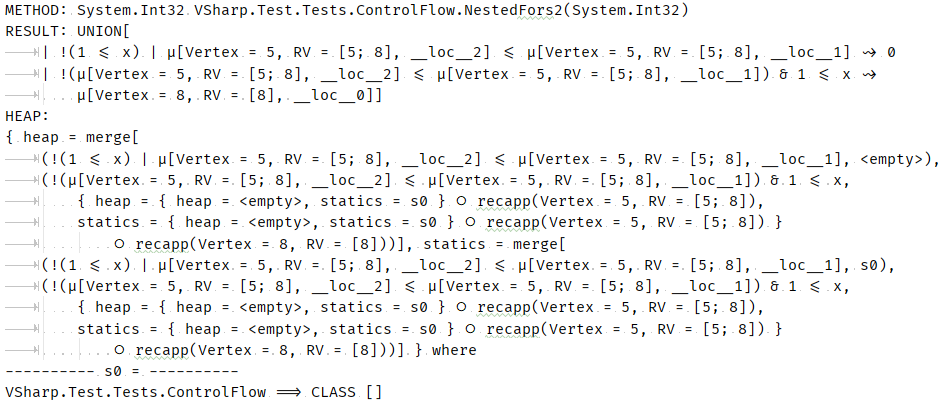
\includegraphics[scale=0.5]{Batoev/images/results.PNG}
\caption{Результат символьного исполнения метода~\ref{example:fors}}
\end{figure}

\begin{table}[t]
    \centering
    \begin{tabular}{ |p{3cm}||p{2cm}|p{2cm}|p{2cm}|  }
        \hline
        \multicolumn{4}{|c|}{Количественные характеристики тестов} \\
        \hline
        Название тестового набора &Количество тестов в наборе&Количество успешно пройденных тестов&Количество инструкций CIL\\
        \hline
        Arithmetics   &80    &77    &1968\\
        Logics        &75    &75    &1458\\
        Conditional   &10    &6     &943\\
        Recursive     &5     &5     &751\\
        Lambdas       &2     &2     &404\\
        Generic       &14    &14    &194\\
        Strings       &15    &15    &219\\
        Unsafe        &16    &16    &312\\
        Typecast      &19    &19    &969\\
        Methods       &10    &10    &238\\
        Lists         &9     &9     &1420\\
        Chess.NET     &1     &1     &2723\\
        \hline
        Всего         &256   &249   &11599\\
        \hline
    \end{tabular}
    \captionof{table}{Результаты тестирования}
    \label{experiments}
\end{table}


\FloatBarrier

\subsection{Тестирование интерпретатора}
Тестирование нового интерпретатора проводилось на тестовой подсистеме проекта <<VSharp.Test>> и на библиотеке \textsc{Chess.NET}.
Подсистема содержит тестовые наборы, затрагивающие различные конструкции и возможности языка C\#:
арифметику, логические операции,
работу с массивами разных размерностей, генерирование исключений, тесты на классы и структуры, включающие взаимодействие со статическими членами и вызовы виртуальных методов,
тесты с неограниченной рекурсией, тесты с \emph{unsafe}-кодом, тесты со строками. 

Таблица~\ref{experiments} показывает результаты проведенного тестирования. 
В наборах тестах с арифметикой и условными конструкциями была часть тестов с генерацией исключений. 
Поскольку схема обработки исключений для языка CIL не была реализована, то данные тесты были некорректно исполнены.
По той же причине не было проведено тестирования на тестовым наборе <<TryCatch>>, 
основное предназначение которого --- инициирование и перехват исключений.

\section{Заключение}

В данной работе описан подход к композициональному символьному исполнению без раскрутки. Была предложена концепция композициональной памяти с символьной адресацией. Был доказан некоторый набор свойств КСП, дающий основание для подхода в стиле систем переписывания, где символьные кучи могут сами выступать как символы. Это даёт возможность автоматически порождать уравнения на состояния, решения которых в точности отражают поведения функций, работающих с динамической памятью. Было показано как свести задачу решения уравнений на состояния к задаче проверки безопасности чистых функций второго порядка.

Данная работа нацелена на теоретические основания композиционального анализа динамической памяти. Мы оставляем апробацию этого подхода на будущее. Другим направлением будущих исследований может быть расширение нашего формализма на композициональный анализ параллельных программ.

\bibliographystyle{ugost2008ls}
\begin{thebibliography}{10}

\bibitem{baldoni2018survey}
Roberto Baldoni, Emilio Coppa, Daniele~Cono D’elia, Camil Demetrescu, and
  Irene Finocchi.
\newblock A survey of symbolic execution techniques.
\newblock {\em ACM Computing Surveys (CSUR)}, 51(3):50, 2018.

\bibitem{godefroid2007compositional}
Patrice Godefroid.
\newblock Compositional dynamic test generation.
\newblock In {\em ACM Sigplan Notices}, volume~42, pages 47--54. ACM, 2007.

\bibitem{jaffar2012tracer}
Joxan Jaffar, Vijayaraghavan Murali, Jorge~A Navas, and Andrew~E Santosa.
\newblock Tracer: A symbolic execution tool for verification.
\newblock In {\em International Conference on Computer Aided Verification},
  pages 758--766. Springer, 2012.

\bibitem{king1976symbolic}
James~C King.
\newblock Symbolic execution and program testing.
\newblock {\em Communications of the ACM}, 19(7):385--394, 1976.

\bibitem{kuznetsov2012efficient}
Volodymyr Kuznetsov, Johannes Kinder, Stefan Bucur, and George Candea.
\newblock Efficient state merging in symbolic execution.
\newblock {\em Acm Sigplan Notices}, 47(6):193--204, 2012.

\bibitem{mcmillan2010lazy}
Kenneth~L McMillan.
\newblock Lazy annotation for program testing and verification.
\newblock In {\em International Conference on Computer Aided Verification},
  pages 104--118. Springer, 2010.

\bibitem{kostyukov2018csewu}
Юрий~Олегович Костюков.
\newblock {\em Кучи как чистые функции:
  композициональное символьное исполнение
  без раскрутки}, pages 288--346.
\newblock 6. 2018.

\end{thebibliography}

\title{Композициональное символьное исполнение CIL-кода}

\titlerunning{Композициональное символьное исполнение CIL-кода}

\author{Батоев Константин Аланович}

\authorrunning{К.~А.~ Батоев}

\tocauthor{Константин Батоев}
\institute{St Petersburg State University\\
	\email{konstantin.batoev@gmail.com}}

\maketitle

% \renewcommand{\ttdefault}{cmtt}

\newsavebox\CBox
\newcommand\hcancel[2][0.1pt]{%
  \ifmmode\sbox\CBox{$#2$}\else\sbox\CBox{#2}\fi%
  \makebox[0pt][l]{\usebox\CBox}%
  \textcolor{red}{\rule[0.3\ht\CBox-#1/2]{\wd\CBox}{#1}}}

\captionsetup[figure]{name=Рисунок}

% \newtheorem*{proof}{Доказательство}

\renewcommand{\defnautorefname}{опр.}
\renewcommand{\lemautorefname}{лемм.}
\renewcommand{\remkautorefname}{зам.}
\renewcommand{\propautorefname}{св.}
\renewcommand{\exmpautorefname}{пр.}
\renewcommand{\thmautorefname}{теор.}
% \renewcommand{\crlrautorefname}{Corollary}
\renewcommand{\sectionautorefname}{разд.}
\newcommand{\algorithmautorefname}{лист.}
\newcommand{\algorithmcfname}{Листинг}
\makeatletter
\renewcommand{\ALG@name}{Листинг}
\makeatother

\algrenewcommand\alglinenumber[1]{\tiny #1:}

\lstdefinelanguage{Demo}
{
 morecomment = [l]{//}, 
 sensitive = true,
 morekeywords = {type, new, null,
   bool, int, write, read,
   fail, nop, let, alloc, in,
   if, then, else, call,
   true, false, and, or, not}
}

\definecolor{commentgreen}{RGB}{0,200,100}
\lstdefinestyle{demolang}{language=Demo,
    rulecolor=\color{blue!80!black},
    basicstyle=\ttfamily\footnotesize,
    keywordstyle=\color{blue}\ttfamily,
    stringstyle=\color{red}\ttfamily,
    commentstyle=\color{commentgreen}\ttfamily,
    numbers=left,
    numbersep=5pt,
    numberstyle=\tiny\color{black},
    escapechar=@,
    tabsize=2
}

\usemintedstyle{vs}

\counterwithin{lstlisting}{section}
\counterwithin{algocf}{section}

\fontfamily{times}
% \fontsize{10pt}{30pt}
\selectfont
\setlength{\parindent}{0em}
% \setlength{\parskip}{1em}
\renewcommand{\baselinestretch}{1.0}

\SetupFloatingEnvironment{listing}{name=Листинг}
\providecommand*{\listingautorefname}{лист.}
\renewcommand*{\figureautorefname}{рис.}
\renewcommand*{\tableautorefname}{табл.}
\SetAlgorithmName{Листинг}{лист.} 

\theoremstyle{plain}
\newtheorem{thm}{Теорема}%[section]
\newtheorem{lem}{Лемма}%[section]
% \newtheorem{crlr}{Corollary}%[section]

\theoremstyle{definition}
\newtheorem{defn}{Определение}
\newtheorem{remk}{Замечание}
\newtheorem*{remk*}{Замечание}
\newtheorem{prop}{Утверждение}
\newtheorem{exmp}{Пример}
% \newtheorem*{proof}{Доказательство}

% \newcommand{\defnautorefname}{опр.}
\newcommand{\lemautorefname}{лем.}
\newcommand{\remkautorefname}{зам.}
\newcommand{\propautorefname}{утв.}
\newcommand{\exmpautorefname}{пример}
\newcommand{\thmautorefname}{теор.}
% \renewcommand{\crlrautorefname}{Corollary}
\renewcommand{\sectionautorefname}{секция}
% \renewcommand{\algorithmautorefname}{Алгоритм}
% \renewcommand{\algorithmcfname}{Алгоритм}

% \renewcommand*{\Authsep}{\authorcr}
% \renewcommand*{\Authand}{\authorcr}
% \renewcommand*{\Authands}{\authorcr}

% \makeatletter
% \makeatother

\lstdefinelanguage{Demo}
{
 morecomment = [l]{//}, 
 sensitive = true,
 morekeywords = {new, null,
   fail, goto, halt,
   true, false, and, or, not}
}

\definecolor{commentgreen}{RGB}{0,200,100}
\lstdefinestyle{demolang}{language=Demo,
    rulecolor=\color{blue!80!black},
    basicstyle=\ttfamily\footnotesize,
    keywordstyle=\color{blue}\ttfamily,
    stringstyle=\color{red}\ttfamily,
    commentstyle=\color{commentgreen}\ttfamily,
    numbers=left,
    numbersep=5pt,
    numberstyle=\tiny\color{black},
    escapechar=@,
    tabsize=2
}

%%% For graph drawing
\definecolor {processblue}{cmyk}{0.96,0,0,0}
\definecolor {processgreen}{cmyk}{1,0,1,0}
\definecolor {processred}{cmyk}{0, 0.84, 0.80, 0.19}
\definecolor {processyellow}{cmyk}{0, 0, 1, 0}


%\newcommand{\csharp}[1]{\mintinline{csharp}{#1}}

\newcommand{\pex}{\textsc{Pex}}
\newcommand{\predator}{\textsc{Predator}}
\newcommand{\dotnet}{\textsc{.NET}}
\newcommand{\clang}{\textsc{C}}
\newcommand{\vsharp}{\textsc{V\#}}

\newcommand\addrset{loc}
\newcommand\termset{term}
\newcommand\guardset{guard}

\newcommand\eqby[1]{\mathrel{\stackrel{\mbox{\normalfont\tiny #1}}{=}}}
\newcommand\eqdef{\eqby{def}}

\newcommand\aite{ite}
\newcommand\ite[3]{\aite(#1,#2,#3)}
\newcommand\Ite[3]{\aite\big(#1,#2,#3\big)}
\newcommand\pair[2]{\langle#1, #2\rangle}
\newcommand\paiR[2]{\big\langle#1, #2\big\rangle}
\newcommand\mg[2]{#1=#2}
\newcommand\nmg[2]{#1\neq#2}
\newcommand\li[1]{LI(#1)}
\let\emptyheap\varepsilon
\newcommand\agrec{Rec}
\newcommand\agmerge{Merge}
\newcommand\agcompose{\bigcirc}
\newcommand\GRec[1]{\agrec\big(#1\big)}
\newcommand\GMerge[1]{\agmerge\big(#1\big)}
\newcommand\GCompose[2]{#1\agcompose#2}
\newcommand\agho{App}
\newcommand\gapp[1]{\agho(#1)}
\newcommand\GApp[1]{\agho\big(#1\big)}
\newcommand\aunion{\texttt{UNION}}
\newcommand\union[1]{\aunion\big(#1\big)}
\newcommand\Union[1]{\aunion\Big(#1\Big)}
\newcommand\aderef{readStore}
\newcommand\readTerm{readTerm}
\newcommand\writeTerm{writeTerm}
\newcommand\afind{find}
\newcommand\find[5]{\afind(#1,#2,#3,#4,#5)}
\newcommand\finD[5]{\afind\big(#1,#2,#3,#4,#5\big)}
\newcommand\Find[5]{\afind\Big(#1,#2,#3,#4,#5\Big)}
\newcommand\deref[2]{\aderef(#1,#2)}
\newcommand\Deref[2]{\aderef\big(#1,#2\big)}
\newcommand\compose[2]{#1\circ#2}
\newcommand\lmbd[2]{\lambda #1.#2}
\newcommand\lmbdx[1]{\lambda x.#1}
\newcommand\dom[1]{dom(#1)}
\newcommand\Dom[1]{dom\big(#1\big)}

\newcommand\Li[1]{LI\big(#1\big)}
\newcommand\amutate{writeStore}
\newcommand\amutateStack{writeStack}
\newcommand\mutate[3]{\amutate(#1,#2,#3)}
\newcommand\mutateStack[4]{\amutateStack(#1,#2,#3,#4)}
\newcommand\rdbodyext[6]{\Union{\big\{\paiR{#4\mg{#1}{#5}}{#6\big(#2(#5), xs\big)} \mid #5\in\dom{#2} \big\}\\&\qquad\qquad\qquad\cup\paiR{#4\bigwedge_{\mathclap{#5\in\dom{#2}}}{\nmg{#1}{#5}}}{#6\big(#3, xs\big)}}}
\newcommand\rdbody[4]{\rdbodyext{#1}{#2}{#3}{}{l}{#4}}
\newcommand\wrtbody[6]{\Union{&\paiR{\mg{#1}{#2}}{\writeTerm\big(#3,#4,#6\big)},
    \\&\paiR{\nmg{#1}{#2}}{\writeTerm\big(#5(#1),#4,#6\big)}}}
\newcommand{\var}[1]{\mathit{#1}}


\begin{abstract}
Известно, что наибольшую сложность в области верификации программ представляет задача доказательства корректности программ с циклическими участками кода. Опираясь на подход символьного исполнения программ и на введенные формализмы обобщённых куч в работе~\cite{kostyukov2018csewu}, данная работа представляет алгоритм композиционального символьного исполнения без раскрутки отношения перехода программ с произвольным графом потока управления. На его основе был реализован символьный интерпретатор языка CIL в проекте V\#, символьной виртуальной машине для анализа .NET. Была проведена апробация алгоритма на примерах, включающих сложные потоки управления, и интерпретатора на тестовой базе проекта VSharp.Test и на библиотеке Chess.NET.
\end{abstract}
\section*{Введение}
Поиск путей в графе с ограничением в виде формальных языков~\cite{FLCpathProblem} --- это задача, в которой формальные языки используются для задания множества искомых путей. В таком подходе каждый путь соответствует слову, состоящему из меток его рёбер, а ограничением на путь является принадлежность соответствующего ему слова некоторому заданному формальному языку.

В качестве класса формальных языков по иерархии Хомского наибольший интерес представляют контекстно-свободные языки. В отличие от регулярных они обладают большей выразительностью. Поэтому в задаче поиска путей контекстно-свободные ограничения позволяют задавать более сложные отношения между вершинами. Так, например, важный класс запросов поиска вершин, лежащих на одном уровне иерархии~\cite{zhlang-2016}, задаётся только контекстно-свободными, но не регулярными ограничениями. Запросы такого вида, как и другие запросы с контекстно-свободными ограничениями имеют широкое применение в биоинформатике~\cite{bio-application} и при обработке rdf-файлов~\cite{zhlang-2016}.

Наиболее удобным и подходящим инструментом для работы с граф\-структурированными данными являются графовые базы данных. Так же как и реляционные, графовые базы данных поддерживают свой язык запросов. С его помощью графовые базы данных позволяют решать вышеупомянутую задачу поиска путей. Но ограничения на пути, которые поддерживается в наиболее распространённых базах данных, являются в лучшем случае регулярными.

Отсутствие поддержки контекстно-свободных ограничений в графовых базах данных, во-первых, сильно ограничивает выразительность языка запросов. Во-вторых, при необходимости в более сложных запросах разработчикам приходится самим писать алгоритмы, решающие задачу контекстно-свободной достижимости для их частного случая. Так, например, Хуэй Мяо и др.~\cite{datascince-lifecycle} разработали систему хранения и отслеживания версий артефактов, возникающих при научных работах. Вся информация про артефакты хранилась в графовой базе данных. При этом при разработке возникла потребность в выполнении запросов с контекстно-свободными ограничениями для выявления взаимоотношений между различными версиями различных артефактов. Это и послужило началом статьи~\cite{datascince-lifecycle}, в которой приводятся алгоритмы решения частных запросов.

В недавнем исследовании Йохем Куйперс и др.~\cite{Kuijpers:2019:ESC:3335783.3335791} произвели сравнительный анализ наиболее известных алгоритмов поиска путей с конте\-кстно-свободными ограничениями. Алгоритмы запускались на графах, находящихся в хранилище графовой базы данных Neo4j. По результатам исследования было показано, что в контексте Neo4j алгоритмы обладают большим временем работы, и поэтому дальнейшая работа по расширению языка запросов прекратилась. При этом Рустам Азимов~\cite{Azimov:2018:CPQ:3210259.3210264} предоставил матричный алгоритм и его реализацию, которая работает за разумное время на реальных данных. Но, так как алгоритм был реализован вне контекста базы данных, его результат приняли недостаточно показательным. Поэтому вопрос о реализуемости запросов с контекстно-свободными ограничениями в графовых базах данных, а соответственно и о возможности расширения языка запросов для их поддержки остаётся открытым.

\section{Постановка задачи}
Целью данной работы является полная поддержка запросов с конте\-кстно-свободными ограничениями для графовой базы данных. А именно, необходимо предоставить пользователю возможность формулировать запросы с контекстно-свободными ограничениями в терминах одного из существующих стандартных языков запросов и исполнять их в графовой базе данных за приемлемое время. Для достижения этой цели были поставлены следующие задачи.

\begin{itemize}
    \item Выполнить обзор существующих реализаций поддержки запросов с контекстно-свободными ограничениями в графовых базах данных. В результате обзора необходимо выбрать наиболее перспективный с точки зрения производительности алгоритм решения задачи контекстно-свободной достижимости и подходящую для его интеграции базу данных. При выборе базы данных необходимо учитывать как возможность интеграции выбранного алгоритма, так и возможность поддержки одного из стандартных языков запросов, позволяющего выражать контекстно-свободные ограничения.
    \item Интегрировать выбранный на предыдущем шаге алгоритм в выбранную графовую базу данных.
    \item Расширить язык запросов выбранной базы данных конструкциями, необходимыми для выражения контекстно-свободных ограничений.
    \item Произвести замеры производительности полученного решения и сравнить его с существующими решениями.
\end{itemize}


\section{Обзор}

\subsection{Терминология}
Контекстно-свободной грамматикой называется $G = (\Sigma, N, P, S)$, где $\Sigma$ --- алфавит терминальных символов, $N$ --- алфавит нетерминальных символов, $P$ --- множество правил вида $A \rightarrow \alpha$, где $A \in N$, $\alpha \in (\Sigma \cup N)^*$, а $S \in N$ --- выделенный стартовый нетерминал.

% \gsv{про S забыли}.

Языком $L$ над алфавитом $\Sigma$ называется любое подмножество $2^{\Sigma^*}$. Языком, порождаемой грамматикой G, является множество $L(G) = \{S \xRightarrow{*} \beta, \beta \in \Sigma^*\}$, где $S \xRightarrow{*} \beta$ означает, что из нетереминала $S$ путём последовательного применения правил грамматики выводится $\beta$.

Контекстно-свободная грамматика $G = (\Sigma, N, P, S)$ находится в осла\-бленной нормальной форме Хомского, если любое её правило имеет вид $A \rightarrow BC$, где $A, B, C \in N$, либо $A \rightarrow a$, где $A \in N, a \in \Sigma$. В отличие от нормальной формы Хомского в ослабленной, во-первых, допускается присутствие стартового нетерминала $S$ в правых частях правил грамматики, во-вторых, запрещаются правила вида $S \rightarrow \epsilon$, где $\epsilon$ --- пустая строка.

% \gsv{Это не нормальная форма Хомского. У НФХ есть дополнительные ограничения. Мы называем то, что здесь, ослабленной НФХ. Важно отдельно проговорить разницу с НФХ.}

В задаче поиска путей с ограничениями в виде формальных языков дан граф $(V, E)$, разметка его рёбер $l: E \rightarrow \Sigma$ и язык $L$ над алфавитом $\Sigma$. Требуется найти множество всех пар вершин, между которыми существует путь, метки на рёбрах которого образуют слово в заданном языке. То есть требуется найти следующее множество:
\[\{(v, to): \exists p=(e_1,...,e_n) \in E^*: l(e_1)...l(e_n) \in L,~src(e_1)=v,~dst(e_n)=to\}\]
Здесь $src(e)$ и $dst(e)$ для $e \in E$ означают начальную и конечную вершину ребра $e$. В данном контексте язык $L$ называется языком ограничений.
% \gsv{У Вас вершины v и to никак с путём не связаны}

Задача поиска путей с контекстно-свободными ограничениями --- это задача поиска путей в виде формальных языков, в которой язык задаётся контекстно-свободной грамматикой.

\subsection{Графовые базы данных}
Графовые СУБД\footnote{СУБД --- Система управления базами данных} (далее просто графовые базы данных) --- это разновидность СУБД, в которой данные хранятся в виде графов. В отличие от других разновидностей, в графовых базах данных отношения между объектами так же важны, как и сами объекты.

Основной моделью представления графов в таких базах данных является gpraph property model~\cite{graph-propery-model}. В ней каждая сущность может содержать набор свойств в формате ключ-значение. Основными сущностями являются узлы и отношения. Узлы соответствуют вершинам графа и помимо свойств могут иметь несколько меток. Отношения соответствуют рёбрам и имеют ровно одну метку, которая называется типом отношения. На рисунке~\ref{fig:graph_bd_1} показан небольшой пример графа в такой модели. 

\begin{figure}[h]
\centering
    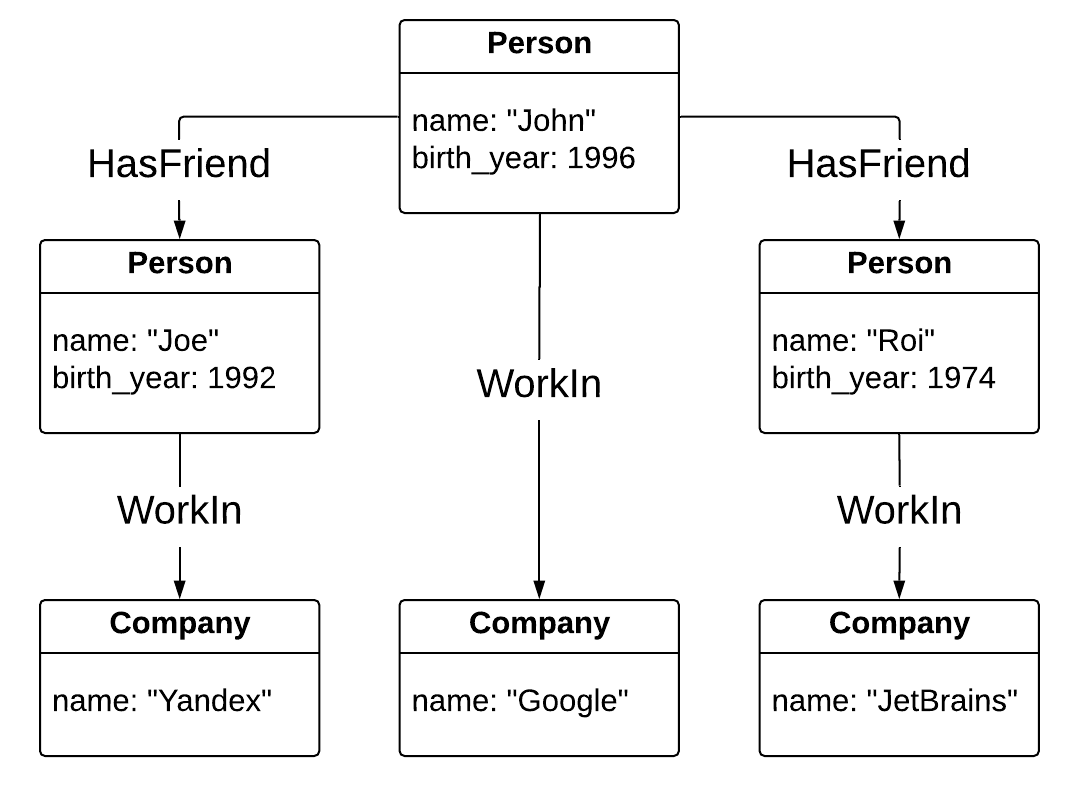
\includegraphics[width=0.7\linewidth]{Terekhov/pictures/graph_bd_1.png}
    \caption{Пример социального графа}
    \label{fig:graph_bd_1}
\end{figure}

Для работы с графами графовые базы данных предоставляют язык запросов, самым популярным из которых является Cypher~\cite{cypher-language}. В нём главный интерес представляют запросы вида сопоставления с образцом. Они позволяют задавать интересующие пути или подграфы в виде шаблонов и описывать информацию, которую нужно извлечь после удачного сопоставления. На рисунке~\ref{code:cypher_query} приведён пример такого запроса. Шаблон пути описывается в выражении MATCH. В нём между круглыми скобками задаются шаблоны вершин, а между квадратными шаблоны рёбер. Таким образом в данном примере задаются следующие ограничения: путь должен начинаться из вершины с меткой Person и именем John и состоять из двух рёбер, первое из которых должно иметь тип HasFriend, а второе WorkIn. В выражении RETURN задаётся информация, которую нужно извлечь. В данном примере это имя последней в пути вершины. В итоге ответом на такой запрос являются имена компаний, в которых работают друзья Джона. Результатом работы этого запроса на графе из рисунка~\ref{fig:graph_bd_1} является множество \{"Yandex", "JetBrains"\}.

%\lstset{
%   basicstyle=\fontsize{14}{14}\selectfont\ttfamily
%}

\begin{figure}[h]
\begin{lstlisting}[language=sql]
MATCH (p:Person)-[:HasFriend]->()-[:WorkIn]->(to)
WHERE p.name = "John"
RETURN to.name
\end{lstlisting}
\caption{Пример конечного запроса на языке Cypher}
\label{code:cypher_query}
\end{figure}

С формальной точки зрения шаблоны пути в выражении MATCH позволяют поставить задачу поиска путей с ограничениями в виде формальных языков. Так в запросе на рисунке~\ref{code:cypher_query} языком ограничений является конечный язык $\{(HasFriend, WorkIn)\}$. Для запроса на рисунке~\ref{code:cypher_query_2} ограничением является регулярный язык $\{A, B\}^*$. 

\begin{figure}[h]
\begin{lstlisting}[language=sql]
MATCH (v)-[:A | :B *]->(to)
RETURN to.name
\end{lstlisting}
\caption{Пример регулярного запроса на языке Cypher}
\label{code:cypher_query_2}
\end{figure}

При этом регулярные ограничения поддерживаются лишь частично и позволяют искать только пути произвольной длины с заданными метками на рёбрах, а более глубокие регулярные выражения не поддерживаются. Поэтому на текущий момент язык запросов довольно ограничен.

\subsection{Существующие решения}
Как было упомянуто раннее, ни одна графовая база данных не поддерживает запросов с контекстно-свободными ограничениями. Тем не менее существуют альтернативные решения поддержки таких запросов. 

\subsubsection{Парсер-комбинаторы для Neo4j}\label{sec:pareser-combinators}
В 2018 году группой исследователей из JetBrains Research на основе библиотеки Meerkat была разработана библиотека для поддержки запросов с контекстно-свободными ограничениями~\cite{parser-combinators}. Она использует графовую базу данных Neo4j~\cite{neo4j} как хранилище графов и позволяет задавать запросы в виде парсер-комбинаторов. Основным достоинством данной работы является то, что с помощью этой библиотеки кроме контекстно-свободных запросов можно выразить базовую часть языка Cypher. Но так как конкурировать с оригинальной реализацией выполнения запросов Neo4j очень сложно, это достигается вместе c сильной потерей производительности. Кроме этого контекстно-свободные запросы обрабатываются также достаточно медленно.

Таким образом данное решение является альтернативой языка запросов Neo4j, а не его расширением. Из-за медленного времени работы такое решение подходит только для работы с небольшими графами. 

\subsubsection{Расширение языка запросов SPARQL}\label{subsection:cypher-extention-2}
%Про sparql%
В 2016 Сяованг Чжан предоставил язык cfSPARQL~\cite{zhlang-2016} --- расширение языка SPARQL, который способен выразить запросы с контекстно-свободными ограничениями. Также он привёл алгоритм для вычисления таких запросов и замеры производительности. Но, во-первых, работа была сделана вне контекста графовой базы данных, а во-вторых, время работы предложенного алгоритма было больше, чем время работы парсер-комбинаторов.

\subsubsection{Существующие реализации алгоритмов решения задачи контекстно-свободной достижимости}
Основной сложностью расширения языка запросов для поддержки запросов с контекстно-свободными ограничениями является долгое время работы соответствующих алгоритмов. Так, например, в 2019 году Йохем Куйперс и другие исследователи с целью попытки расширения языка запросов Cypher для графовой базы данных Neo4j произвели сравнительный анализ производительности наиболее известных алгоритмов решения задачи контекстно-свободной достижимости.

В данном исследовании были рассмотрены и произведены замеры времени работы алгоритма Элле Хелингса~\cite{hellings-2015}, основанного на атрибутных грамматиках, восходящего алгоритма Фреда Сантоса~\cite{santos-2018}, матричного алгоритма Рустама Азимова~\cite{Azimov:2018:CPQ:3210259.3210264} и алгоритма Петтери Севона~\cite{bio-application}. Все алгоритмы были интегрированы в Neo4j и запускались на графах, находящихся в её хранилище. Алгоритмы были написаны на языке Java, при этом их реализация являлась однопоточной.

% \gsv{В таких местах надо сразу ссылку на алгоритм давать.}

По результатам замеров производительности было показано, что время работы алгоритмов является слишком большим и неприемлемым для широкого практического использования. Поэтому дальнейшая работа по интеграции и расширению языка запросов была приостановлена.

Тем не менее, матричный алгоритм Рустама Азимова в сравнительном анализе Йохема Куйперса был реализован без необходимых матричных библиотек, которые могут сильно уменьшить время его работы. Так, например, в исследовании Никиты Мишина и др.~\cite{azimov-evalution} был произведён сравнительный анализ времени работы нескольких реализаций алгоритма Рустама Азимова, основанных на различных специализированных матричных библиотеках. Графы и запросы к ним были взяты из объемлющего набора данных CFPQ\_Data~\cite{cfpq-data}, предоставленного лабораторией языковых инструментов JetBrains Research. 

Результаты замеров Никиты Мишина и др. показали, что при грамотной реализации алгоритма Рустама Азимова и использовании подходящих матричных библиотек можно добиться очень высокой производительности. Поэтому, так как основной проблемой применимости запросов с контекстно-свободными ограничениями является долгое время работы соответствующих алгоритмов, в качестве алгоритма решения задачи конте\-кстно-свободной достижимости был выбран матричный алгоритм Рустама Азимова.

\subsection{Матричный алгоритм Рустама Азимова}\label{sec:matrix-algo}
Выбранный в предыдущей главе алгоритм Рустама Азимова~\cite{Azimov:2018:CPQ:3210259.3210264}, в отличие от других алгоритмов решения задачи контекстно-свободной достижимости~\cite{hellings-2015, santos-2018, zhlang-2016}, работает с графами в виде разреженных матриц смежности. Данный алгоритм состоит из последовательности операций над разреженными матрицами, время работы которых зависит не от размеров матричных операндов, а от количества их ненулевых элементов.

На вход алгоритму (см. алгоритм 1) поступает помеченный граф $D=(V,E)$ и контекстно-свободная грамматика $G=(\Sigma, N, P, S)$ в ослабленной нормальной форме Хомского. Для каждого нетерминала $A$ в ассоциативном массиве $T$ хранится соответствующая ему булева матрица $T[A]$. На всём этапе алгоритма поддерживается следующий инвариант: $T[A]_{i,j} = 1$ равносильно существует пути, метки на рёбрах которого образуют слово, выводящееся из нетерминала $A$. На первом этапе происходит инициализация матриц с помощью простых правил грамматики, после чего инвариант выполняется для всех путей единичной длины. На втором этапе происходит транзитивное замыкание, после чего этот инвариант верен для всех путей. Результатом данного алгоритма является матрица, соответствующая стартовому нетерминалу $S$.

%  Это позволяет для его реализации использовать многопоточные матричные библиотеки, с помощью которых можно добиться очень высокой производительности. Поэтому на текущий момент алгоритм Рустама Азимова показывает наилучшее время работы на практике.

\begin{algorithm}
\caption{Матричный алгоритм Рустама Азимова}

\begin{algorithmic}[1]
\Function{contextFreePathQuerying}{$D$, $G$}
    \State{$n =$ getNodeCount(D)}
    \State{$N =$ getAllNonterms(G)}
    \State{$E =$ getEdges($D$)}
    \State{$P =$ getRules($G$)}
    \State{$S =$ getStartNonterm($G$)}
    \State{$T = \{A \rightarrow \varnothing_{n \times n} : A \in$ $N$ \} }
    \ForAll{$(v, to, label) \in E$}
    \Comment{Инициализация матриц}
        \ForAll{$A \rightarrow label \in P$}
            \State{$T[A]_{i,j} = 1$}
        \EndFor
    \EndFor    
    \While{$\exists A: T[A]$ is changing}
    \Comment{Вычисление замыкания}
        \ForAll{$A \rightarrow BC \in P$}
            \State{$T[A] \oplus= T[B] \otimes T[C]$}
        \EndFor
    \EndWhile
\State \Return $T[S]$
\EndFunction

\end{algorithmic}
\end{algorithm}

Практическое время работы алгоритма Рустама Азимова сильно зависит от производительности используемой матричной библиотеки. Это накладывает некоторые ограничения на выбор подходящей графовой базы данных, так же как и возможность представления графов в матричном виде.

\subsection{RedisGraph}
RedisGraph~\cite{redis-graph} --- это высокопроизводительная графовая база данных, поддерживающая язык запросов Cypher. В отличие от наиболее распространённой графовой базы данных Neo4j~\cite{neo4j}, RedisGraph написан на языке Си и для работы с данными использует Redis~\cite{redis}, основным достоинством которого является возможность хранить данные прямо в оперативной памяти. Это позволяет RedisGraph быстро обрабатывать пользовательские запросы.

Также RedisGraph является единственной графовой базой данных, которая работает с графами в виде разреженных матриц смежности и транслирует запросы языка Cypher в матричные выражения. Для представления графов в таком виде и работы с ними в терминах линейной алгебры используется мощный матричный фреймворк GraphBlas~\cite{graph-blas}. Его реализация SuiteSparse~\cite{suite-sparse} является многопоточной и сильно оптимизирована, что позволяет RedisGraph добиться высокой производительности.

Из всего этого следует, что RedisGraph идеально подходит для интеграции матричного алгоритма. Во-первых, графы представляются в необходимом алгоритму виде, что позволит избежать издержек на конвертацию форматов. Во-вторых, использование SuiteSparse для вычисления матричных операций позволит добиться высокой производительности. Поэтому RedisGraph был выбран в качестве графовой базы данных для интеграции матричного алгоритма и расширения языка запросов.

% Так как алгоритм Рустама Азимова работает с матричным представлением графа,, как наиболее подходящий для интеграции матричного алгоритма.

\subsection{Расширение языка Cypher}\label{subsection:cypher-extention}
На текущий момент оригинальная версия языка Cypher, используемая в том числе и в RedisGraph, не поддерживает запросов с контекстно-свободными ограничениями. Но тем не менее в 2017 году был разработан черновой вариант спецификации расширения Cypher~\cite{cypher-specification}, которая вводит в язык шаблоны путей. Они позволяют выразить более сложные запросы, в том числе запросы с контекстно-свободными ограничениями.

Шаблоны путей являются альтернативой шаблонам рёбер, которые есть в оригинальном Cypher. Они, как и шаблоны рёбер, могут встречаться в выражении MATCH и иметь своё направление. Кроме этого в глобальной области запроса им можно задавать имя, на которое потом можно ссылаться внутри других шаблонов.

Шаблон пути представляет из себя регулярное выражение над некоторыми примитивами. В качестве таких примитивов могут выступать шаблоны рёбер, шаблоны вершин и ссылки на именованные шаблоны путей. Также любым подвыражениям можно задавать своё направление. Основная часть конкретного синтаксиса данного расширения приведена на рисунке~\ref{fig:cypher_syntax}.

\begin{figure}[]
\begin{align*}
\begin{split}
PathPattern     &= ["<"],~"-/",~PathExpression,~"/-",~[">"]\\
PathExpression  &= \{PathAlternative\}\\
PathAlternative &= PathRepetition,~\{"|", PathRepetition\}\\
PathRepetition  &= ["<"],~PathBase,~[">"],~("*")
\end{split}\\
\begin{split}
PathBase &= PathEdge \\
         &~~|~PathNode \\
         &~~|~PathReference \\
         &~~|~"[",~PathExpression,~"]"
\end{split}\\
\begin{split}
PathEdge      &= Label \\
PathNode      &= "(",~[Label,~\{"|",~Label\}],~")" \\
PathReference &= "\sim",~SymbolicName; \\
Label         &= ":",~LabelName
\end{split}
\end{align*}
\caption{Расширение конкретного синтаксиса Cypher}
\label{fig:cypher_syntax}
\end{figure}

Каждый шаблон пути задаёт отношение на множестве вершин. Поэтому семантикой языка шаблонов путей $L_{P}$ в контексте графа $G(V, E)$ является отображение $\llbracket \cdot \rrbracket_{G}: L_P \rightarrow V \times V$, которое каждому шаблону $p\in L_P$ сопоставляет множество пар вершин, между которыми существует путь, удовлетворяющий данному шаблону $p$. 

Подробное описание данной семантики приводится в таблице~\ref{tab:cypher_sematic}.  В ней наибольший интерес представляют именованные шаблоны путей, так как именно с помощью них можно выразить запросы с контекстно-свободными ограничениями. Все именованные шаблоны путей $S_i = p_j$ можно рассматривать как правила контекстно свободной грамматики с алфавитом нетерминалов $\{S_i\}_{i=1}^n$. Тогда каждый нетерминал $S_j$ порождает язык $L_{S_j} \subset L_p$, а семантикой соответствующего именованного шаблона пути $S_j=p_j$ является множество $\bigcup\limits_{p \in L_{s_j}} \llbracket p \rrbracket_{G}$.

На рисунке~\ref{code:cypher_query_3} приведён пример запроса в расширенном синтаксисе. В нём декларируется именованный шаблон S, который задаёт множество правильных скобочных последовательностей над ребрами с типом L и R. Далее в выражении MATCH задаётся шаблон пути, состоящий из ссылки на шаблон S. Таким образом результатом обработки запроса является множество всех пар вершин, между которыми существует путь, метки на рёбрах которого образуют правильную скобочную последовательность. 

\begin{table}[h!]
\begin{adjustbox}{max width=\textwidth}
\begin{tabular}{|c|c|c|}
\hline
$p \in L_P$                                                                                  & $\llbracket p \rrbracket_{G}$                                                                                                                                                                                   & Описание шаблона пути                                                                                                         \\ \hline
\hline
()                                                                                            & $\{(v, v): v \in V\}$                                                                                                                                                                                           & \begin{tabular}[c]{@{}c@{}}Пустой путь, состоящий из \\ одной произвольной вершины\end{tabular}                               \\ \hline
:a                                                                                            & $\{e=(v,to): e \in E, type(e)=a\}$                                                                                                                                                                              & \begin{tabular}[c]{@{}c@{}}Путь единичной длины,\\  состоящий из ребра с типом $a$\end{tabular}                               \\ \hline
(:b)                                                                                          & $\{(v, v): v \in V, label(v)=b\}$                                                                                                                                                                               & \begin{tabular}[c]{@{}c@{}}Пустой путь, состоящий из одной\\  вершины, помеченной меткой $b$\end{tabular}                     \\ \hline
$\alpha~\beta$                                                                                & $\llbracket \alpha \rrbracket_{G}\circ \llbracket \beta \rrbracket_{G}$                                                                                                                                         & Конкатенация путей $\alpha$ и $\beta$                                                                                         \\ \hline
$\alpha~|~\beta$                                                                              & $\llbracket \alpha \rrbracket_{G}\cup \llbracket \beta \rrbracket_{G}$                                                                                                                                          & Альтренатива между путями $\alpha$ и $\beta$                                                                                  \\ \hline
$[\alpha]$                                                                                    & $\llbracket \alpha \rrbracket_{G}$                                                                                                                                                                              & \begin{tabular}[c]{@{}c@{}}Квадратные скобки позволяют \\ группировать  выражения \\ для задания ассоциативности\end{tabular} \\ \hline
\textless{}$\alpha$                                                                           & $\{(to, v): (v, to) \in \llbracket \alpha \rrbracket_{G}\}$                                                                                                                                                     & Путь, обратный к пути $\alpha$                                                                                                \\ \hline
\textless{}$\alpha$\textgreater{}                                                             & $\llbracket \alpha~|~$\textless{}$\alpha \rrbracket_{G} $                                                                                                                                                       & \begin{tabular}[c]{@{}c@{}}Альтернатива между путём $\alpha$ и\\ обратным к нему\end{tabular}                                 \\ \hline
$\alpha^*$                                                                                    & $\llbracket \alpha \rrbracket_{G}^{*}$                                                                                                                                                                          & \begin{tabular}[c]{@{}c@{}}Путь, состоящий из\\ конкатенации 0 или более путей $\alpha$\end{tabular}                          \\ \hline
\begin{tabular}[c]{@{}c@{}}$\{S_i = p_i\}_{i=1}^{n}$\\ -- named\\  path patterns\end{tabular} & \begin{tabular}[c]{@{}c@{}}$P = \{S_i \rightarrow p_i\}_{i=1}^n$\\ $Gram_j = (\Sigma, \{S_i\}_{i=1}^n, P, S_j)$\\ $\llbracket S_j \rrbracket_{G} = \bigcup\limits_{p \in L(G)}{\llbracket p \rrbracket_{G}}$\end{tabular} & Именнованые шалоны путей                                                                                                      \\ \hline
$\sim$$S$                                                                                     & $\llbracket S \rrbracket_{G}$                                                                                                                                                                                   & \begin{tabular}[c]{@{}c@{}}Ссылка на именнованный\\  шаблон пути\end{tabular}                                                 \\ \hline
\end{tabular}
\end{adjustbox}
\caption{Семантика языка шаблонов путей}
\label{tab:cypher_sematic}
\end{table}

\begin{figure}[h!]
\begin{lstlisting}[language=sql]
PATH PATTERN S = ()-/ [:L ~S :R] | [~S ~S] | () /-()
MATCH (v)-/ ~S /-(to)
RETURN v, to
\end{lstlisting}
\caption{Пример запроса в расширенном синтаксисе Cypher}
\label{code:cypher_query_3}
\end{figure}

Данная спецификация расширения Cypher была представлена официальными разработчиками и сильно расширяет выразительность языка, предоставляя удобную возможность выражать запросы как с регулярными, так и с контекстно-свободными ограничениями. Поэтому в моей работе приводится поддержка выполнения запросов именно для этого расширения языка.

% \gsv{Не хватает какого-то чёткого вывода про то, что вот именно это мы и буем использовать.}

\section{Реализация}
По результатам обзора было решено реализовать поддержку расширения языка Cypher, представленную в главе~\ref{subsection:cypher-extention}, для графовой базы данных RedisGraph. За основу алгоритма, решающего задачу поиска путей с контекстно-свободными ограничениями, был взят матричный алгоритм Рустама Азимова, описанный в главе~\ref{sec:matrix-algo}.

% \gsv{И зжесь надо ещё раз подитожить в духе "по результатм обзора было решено сделать то и это с использованием того и сего"}

\subsection{План выполнения запроса}\label{execution-plan}
В RedisGraph основной частью обработки запроса является построение плана его выполнения. Её часть, которая относится к шаблонам путей приведена на рисунке~\ref{fig:execution_plan}. В ней зелёным цветом выделено то, что было добавлено или расширено.

В самом начале, после получения запроса строится его абстрактное синтаксическое дерево \textit{AST}. Далее, из него извлекаются именованные и неименованные шаблоны путей \textit{PathPattern} и \textit{NamedPathPatterns}, после чего они преобразуются в более удобное промежуточное представление \textit{PathExpr}. При этом, для дальнейшего связывания ссылок, именованные шаблоны сохраняются в глобальном контексте запроса \textit{PathPatternCtx}.

На следующем этапе происходит трансляция промежуточных представлений \textit{PathExpr} в матричные выражения \textit{AlgebraicExpression}. В них операндами являются либо матрицы, полученные из указанного в запросе графа \textit{GraphCtx}, либо ссылки на именованные шаблоны путей из \textit{PathPatternCtx}. Основной идеей трансляции является то, что после вычисления матричного выражения получается матрица, которая задаёт то же самое отношение на множестве вершин, что и исходный шаблон пути.

Далее каждое такое выражение формирует новую операцию плана выполнения запроса \textit{CfpqTraverseOp}. При её вычислении сначала происходит запуск расширенной версии матричного алгоритма Рустама Азимова. Он решает задачу контекстно-свободной достижимости, заданной именованными шаблонами путей. После этого все ссылки в матричном выражении заменяются на полученные в ходе алгоритма матрицы и происходит вычисление матричного выражения. Каждая такая операция добавляется в план выполнения запроса.

%  \gsv{Используйте \textit{CfpqTraverseOp} вместо долларов для длинных слов. Они тогда не распадаются из-а лишних пробелов.}

\begin{figure}[H]
\centering
    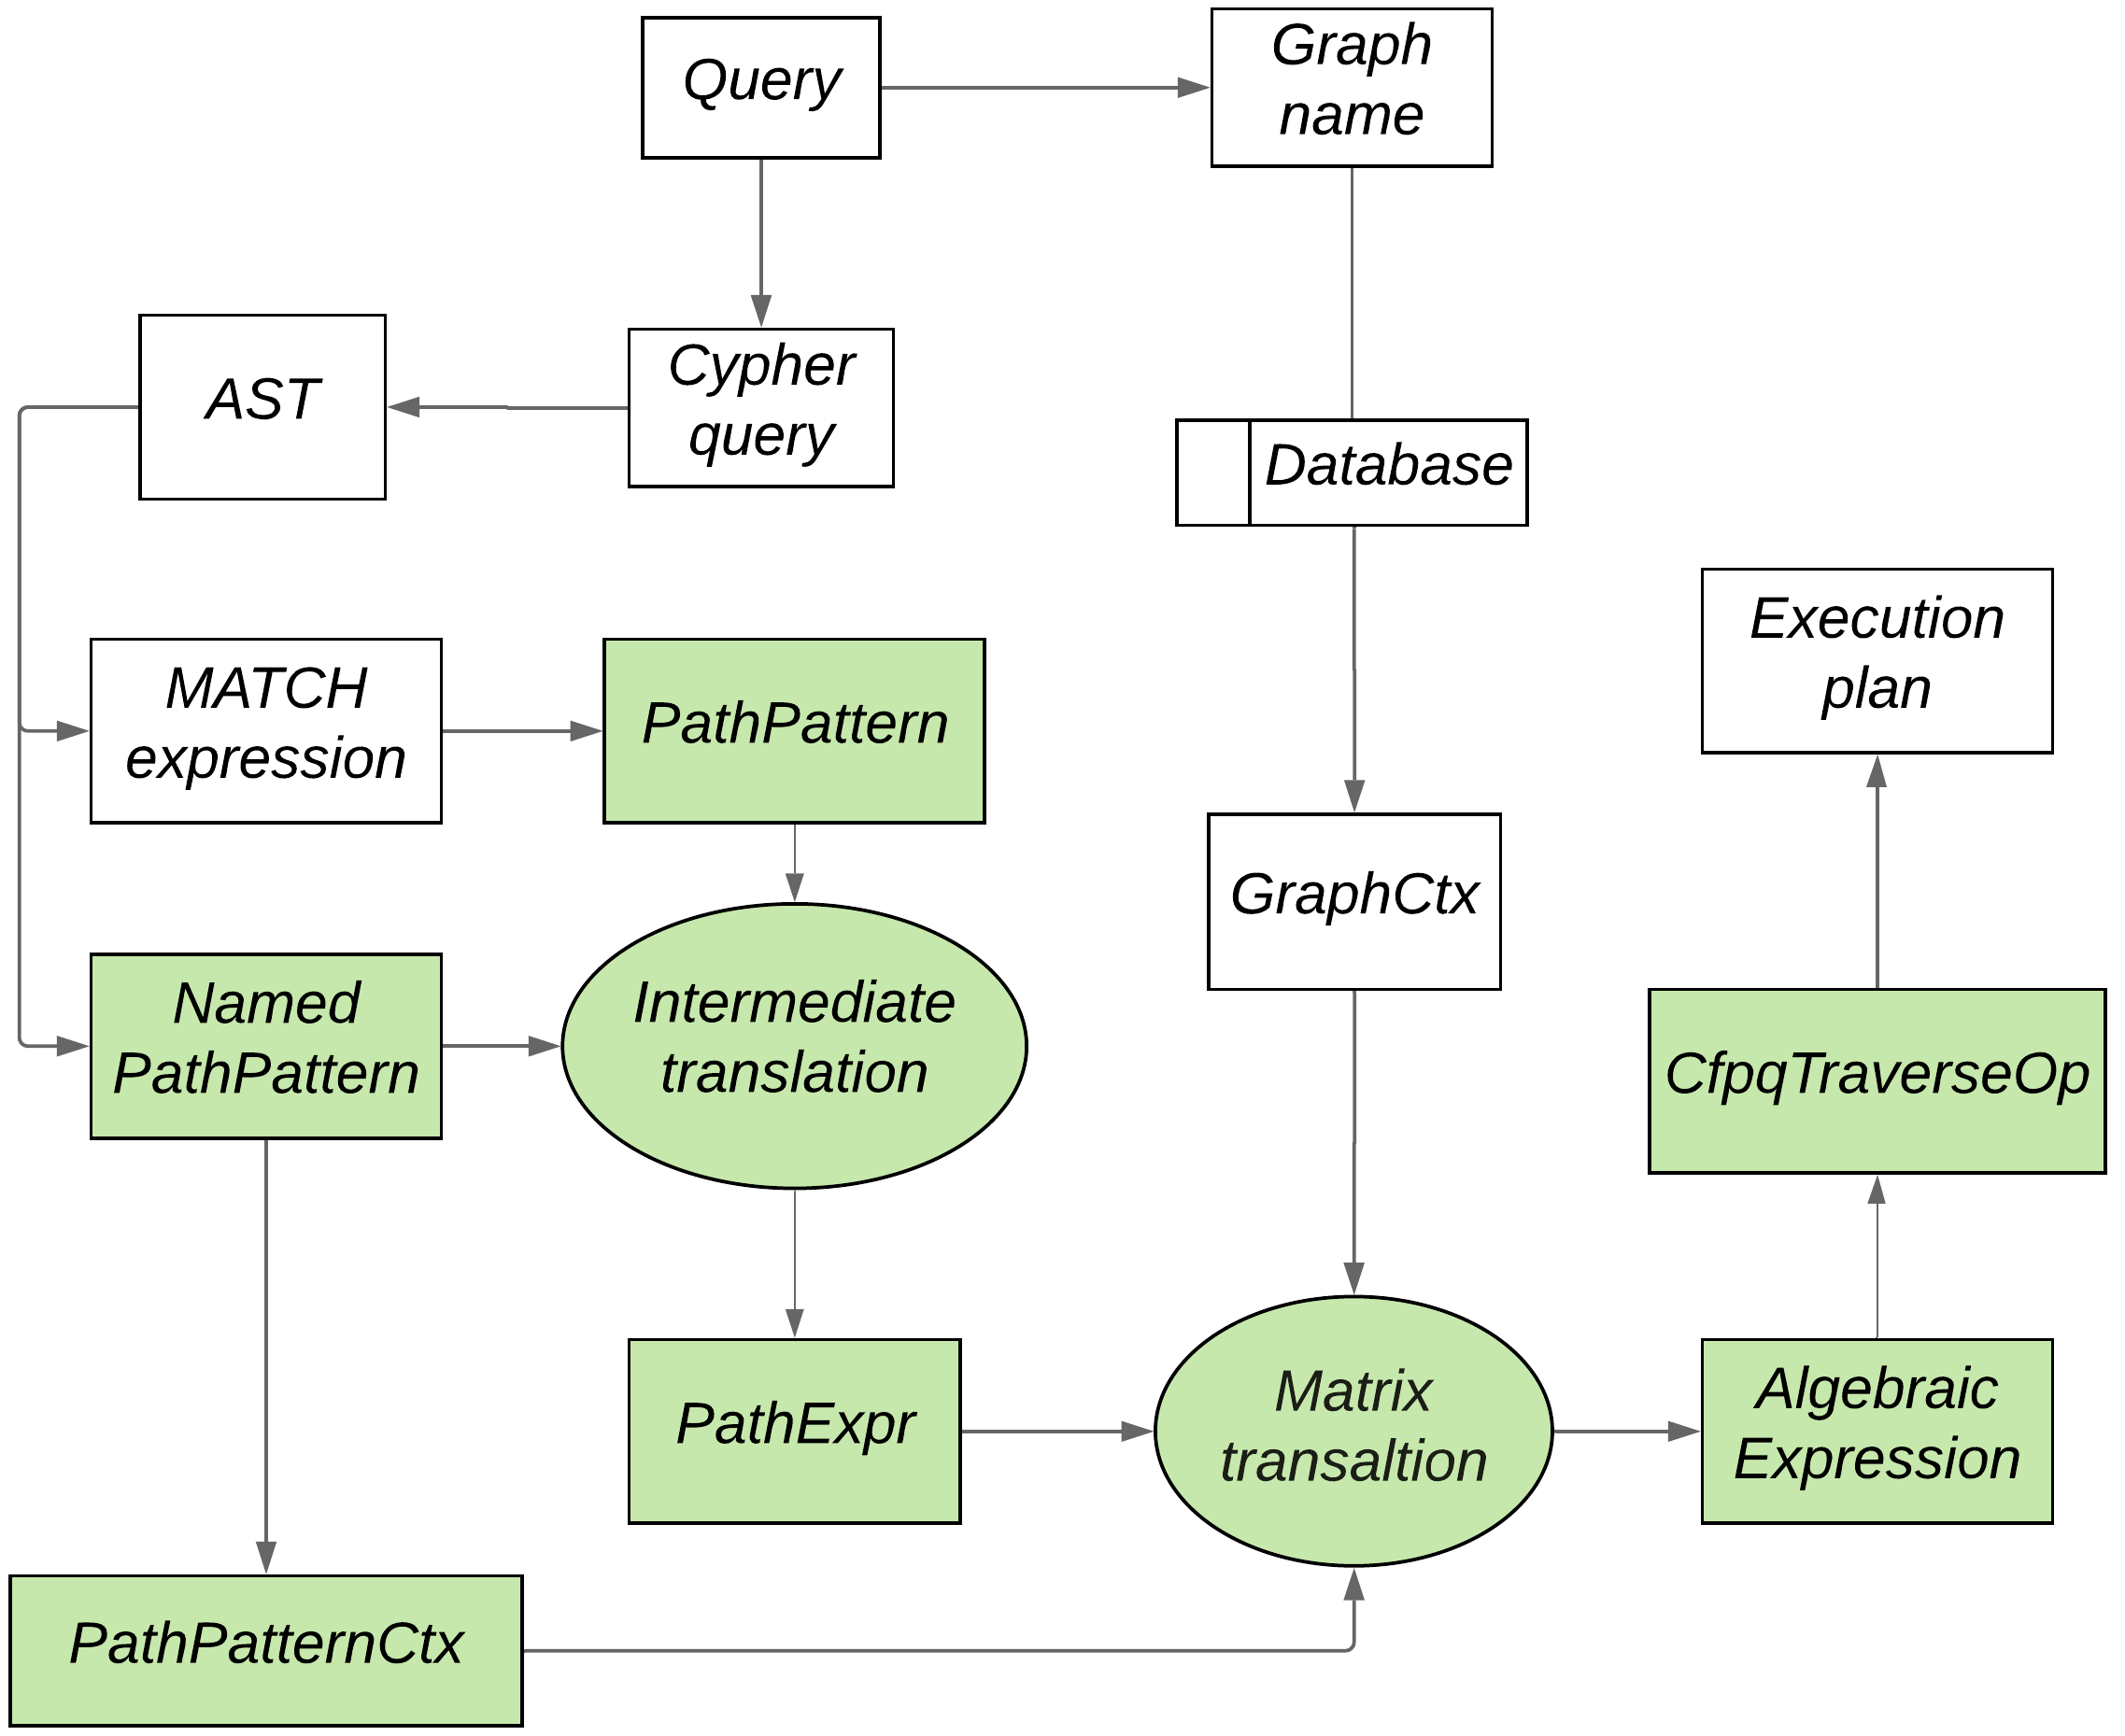
\includegraphics[width=1.0\linewidth]{Terekhov/pictures/execution_plan_3.png}
    \caption{Расширение построения плана выполнения запроса}
    \label{fig:execution_plan}
\end{figure}

\subsection{Промежуточное представление}\label{matrix-translation}
Шаблоны путей, полученные из \textit{AST}, транслируются в промежуточное представление \textit{PathExpr}. Оно позволяет задавать более простой абстрактный синтаксис, который описан на рисунке~\ref{fig:intermidiate_repr}. 

Таким образом, альтернативе и конкатенации шаблонов соответствуют \textit{PathAlt} и \textit{PathSeq}, \textit{PathGroup} позволяет задавать направление пути и наличие замыкания, а \textit{PathBasic} соответствует либо примитивным шаблонам \textit{PathNode}, \textit{PathEdge} и \textit{PathRef}, либо целому выражению \textit{PathExpr}. Примеры промежуточного представления шаблонов приведены в таблице~\ref{tab:inter_examples}.
\begin{figure}[h!]
\begin{align*}
\begin{split}
PathExpr=~ &PathSeq(PathExpr,~PathExpr)~|\\
           &PathAlt(PathExpr,~PathExpr)~|\\
           &PathGroup(PathBasic, direction, range)
\end{split}\\
\begin{split}
PathBasic=~ &PathNode(label)~|\\
            &PathEdge(type)~~|\\
            &PathRef(name) ~~|\\
            &PathExpr
\end{split}\\
\begin{split}
direction \in ~&\{inbound,~outbound,~bidirectional\}\\
range \in     ~&\{*, \varnothing\}
\end{split}
\end{align*}
\caption{Промежуточное представление PathExpr}
\label{fig:intermidiate_repr}
\end{figure}

\begin{table}[h]
\centering
\begin{adjustbox}{max width=\textwidth}
\begin{tabular}{|c|l|}
\hline
$L_p$                        & \multicolumn{1}{c|}{PathExpr}                                                                                                        \\ \hline
{[}:A :B{]} | (:C)           & \begin{tabular}[c]{@{}l@{}}$PathAlt($\\ $~~~~PathSeq(PathEdge("A"),~PathEdge("B"))$\\ $~~~~PathNode("C")$\\ $)$\end{tabular}         \\ \hline
\textless{}{[}:A $\sim$S{]}* & \begin{tabular}[c]{@{}l@{}}$PathGroup($\\ $~~~~PathSeq(PathEdge("A"),~PathRef("S")),$\\ $~~~~inbound,$\\ $~~~~*,$\\ $)$\end{tabular} \\ \hline
\end{tabular}
\end{adjustbox}
\caption{Примеры промежуточного представления запросов}
\label{tab:inter_examples}
\end{table}

\newpage
\subsection{Трансляция в матричные выражения}
Как было упомянуто ранее, RedisGraph представляет графы в виде разреженных матриц. А именно каждый граф $G$ задаётся следующей тройкой $(A \in M_{n\times n},~lab \in Labels \rightarrow Diag_n,~rel \in RelTypes \rightarrow M_{n \times n})_G$. Здесь $M_{n \times n}$ означает полукольцо булевых матриц, а $Diag_n$ полукольцо диагональных булевых матриц. Матрица $A$ служит матрицей смежности графа, а отображения $lab$ и $rel$ сопоставляют меткам вершин и типам рёбер соответствующие булевы матрицы. Таким образом, ребро $(v, to)$ графа $G$ имеет тип $a$ тогда и только тогда, когда $rel(a)_{v,to} = 1$.  Таким же образом, принадлежность метки $l$ вершине $v$ равносильно $lab(l)_{v,v}=1$.

Любую булеву матрицу $M$, участвующую в задании графа $G(V, E)$, можно рассматривать как отношение на множестве вершин $R(M) = \{(v, to):~M_{v,to}=1\}$. Операциями сложения и умножения в булевом полукольце являются дизъюнкция и конъюнкция. Поэтому умножению матриц $A*B$ соответствует композиция отношений $R(A) \circ R(B)$, сложению $A+B$ соответствует объединение отношений $R(A) \cup R(B)$, а транспонированная матрица $A^T$ соответствует обратному к R(A) отношению $R(A)^{-1}$. Такая взаимосвязь между матричными операциями и отношениями лежит в основе алгоритма трансляции, приведённом на рисунке~\ref{algo:translation}.

Данный алгоритм является рекурсивным и принимает на вход промежуточное представление шаблона пути $expr$, представление графа $g$ и контекст именованных шаблонов путей $pathCtx$. Целевым языком трансляции является простой язык матричных выражений, приведённый на рисунке~\ref{fig:alg-expr}.

Базовым случаем рекурсии являются примитивные шаблоны \textit{Path\-Node}, \textit{PathEdge} и \textit{PathReference}, которые транслируются в операнды матричного выражения. Для первых двух соответствующие матрицы извлекаются из графа с помощью функций \textit{GetLabel\-Matrix} и \textit{GetRelation\-Matrix}. При этом случай $label = \varnothing$ соответствует шаблону пути, состоящему из одной произвольной вершины. Поэтому такой путь задаётся тождественным отношением $R(I)$, где $I$ --- единичная матрица. Для \textit{Path\-Reference} создаётся ссылка на матрицу именованного шаблона, которая будет вычислена на следующем этапе при выполнении алгоритма контекстно-свободной достижимости.

Трансляция для шаблонов \textit{PathSeq} и \textit{PathAlt} происходит одинаковым образом --- сначала происходит трансляция дочерних шаблонов, а потом из полученного результата образуются операции умножения или сложения. Такая трансляция обосновывается семантикой шаблонов альтернативы и конкатенации, приведенной в главе~\ref{subsection:cypher-extention}, и связью отношений с матричными операциями, описанными раннее.

Наиболее интересным случаем является трансляция \textit{Path\-Group}, так как в некоторых случаях контекст именованных шаблонов $pathCtx$ расширяется. В начале происходит трансляция дочернего шаблона. Далее, если заданное направление является обратным, к полученной матрице применяется операция транспонирования. Если же направление является произвольным, то формируется операция сложения из полученной матрицы и транспонированной к ней. Это соответствует альтернативе между прямым путём и обратным к нему. После этого при отсутствии замыкания результат возвращается. Иначе происходит трансляция замыкания полученного выражения. Так как его нельзя выразить через имеющиеся матричные операции, создаётся новый именованный шаблон, а замыкание заменяется ссылкой на него. Нетрудно показать, что регулярное выражение $R^*$ и контекстно-свободная грамматика с одним правилом $S \rightarrow R~S \mid \epsilon$ равносильны. Поэтому правая часть этого правила тривиальным образом сразу же транслируется в выражение \textit{Add(Mul(R, MatrixRef(S)), I)} и добавляется в \textit{pathCtx} вместе с полученным новым именем.

Таким образом, после работы данного алгоритма из промежуточного представления шаблона пути получается выражение над матрицами. При дальнейшем его вычислении получается матрица, которая соответствует такому же отношению на множестве вершин, как и семантика изначального шаблона.

\algnewcommand\algorithmicswitch{\textbf{switch}}
\algnewcommand\algorithmiccase{\textbf{case}}
\algnewcommand\algorithmicof{\textbf{of}}
\algnewcommand\algorithmicassert{\texttt{assert}}
\algnewcommand\algorithmiccasepart{\texttt{:}}
\algnewcommand\Assert[1]{\State \algorithmicassert(#1)}%
% New "environments"
\algdef{SE}[SWITCH]{Switch}{EndSwitch}[1]{\algorithmicswitch\ #1}{\algorithmicend\ \algorithmicswitch}%
\algdef{SE}[CASE]{Case}{EndCase}[1]{\algorithmiccase\ #1\algorithmiccasepart}{\algorithmicend\ \algorithmiccase}%
\algdef{SE}[CASEPART]{CasePart}{EndCasePart}[1]{#1\algorithmiccasepart}{\algorithmicend\ \algorithmiccasepart}%
\algtext*{EndSwitch}%
\algtext*{EndCase}%
\algtext*{EndCasePart}%

\begin{algorithm}
\caption{Алгоритм трансляции}
\begin{algorithmic}[1]
\Function{translate}{PathExpr expr, GraphCtx g, PathPatternCtx pathCtx}
    \Switch{expr}
        \Case{$PathNode$(label)}
            \If{label $== \varnothing$}
                \State \Return \Call{GetIdentityMatrix}{g}
            \Else
                \State \Return \Call{GetLabelMatrix}{g, label}
            \EndIf
        \EndCase
        \Case{$PathEdge$(type)}
            \State \Return \Call{GetRelationMatrix}{g, type}
        \EndCase
        \Case{$PathRef(name)$}
            \State \Return $MatrixRef$(name)
        \EndCase
        \Case{$PathSeq$(left, right)}
            \State \Return Add(\Call{translate}{left}, \Call{translate}{right})
        \EndCase
        \Case{$PathAlt$(left, right)}
            \State \Return Mul(\Call{translate}{left}, \Call{translate}{right})
        \EndCase
        \Case{$PathGroup$(basic, dir, range)}
            \State res = \Call{translte}{basic}
            \Switch{dir}
                \Case{$inbound$}
                    \State res = $Transpose$(res)
                \EndCase
                \Case{$bidirectional$}
                    \State res = $Add$(res, $Transpose$(res))
                \EndCase
            \EndSwitch
            \Switch{range}
                \Case{ $\varnothing$}
                    \State \Return res
                \EndCase
                \Case{$*$}
                    \State name = \Call{AllocateNewPathPattern}{ctx}
                    \State res = $Mul$(res, $MatrixRef$(name))
                    \State res = $Add$(res, \Call{GetIdentityMatrix}{g})
                    \State \Call{SetPathPetternExpression}{p, name, res}
                    \State \Return $MatrixRef$(name)
                \EndCase
            \EndSwitch
        \EndCase
    \EndSwitch
\EndFunction
\end{algorithmic}
\caption{Алгоритм транслции в матричные выражения}
\label{algo:translation}
\end{algorithm}

\begin{figure}[H]
\begin{align*}
\begin{split}
AlgExpr= ~ &Add(AlgExpr, AlgExpr)~|\\
           &Mul(AlgExpr, AlgExpr)~|\\
           &Transpose(AlgExpr)~|\\
           &Matrix~|\\
           &MatrixRef(ref)
\end{split}
\end{align*}
\caption{Алгебраическое выражение над матрицами}
\label{fig:alg-expr}
\end{figure}

\subsection{Формирование и вычисление операции плана выполнения}
После этапа трансляции в RedisGraph происходит построение плана выполнения запроса. Он формируется из последовательности операций, которые выполняют базовые вычисления. Для поддержки шаблонов путей была добавлена операция \textit{CfpqTraverseOp}. Она создаётся для каждого матричного выражения, полученного на предыдущем шаге из неименованого шаблона пути, и отвечает за его вычисление.

На этапе инициализации новой операции \textit{CfpqTraverseOp} из соответствующего матричного выражения рекурсивно извлекаются все ссылки на именованные шаблоны путей, от которых зависит данное выражение. После этого они поступают на вход алгоритма, решающего задачу контекстно-свободной достижимости (см. алгоритм 4).

Этот алгоритм является расширенной версией матричного алгоритма Рустама Азимова, приведенного в главе~\ref{sec:matrix-algo}. В данном алгоритме, в отличие от алгоритма Рустама Азимова, не требуется задавать правила грамматики в ослабленной нормальной форме Хомского. Вместо этого правая часть правила задаётся с помощью промежуточного представления \textit{PathExpr}. При этом подразумевается, что для любого именованного шаблона $p$ из глобального контекста \textit{pathCtx} его промежуточное представление уже транслировано в матричное выражение и записано в \textit{pathCtx[p].algExpr}.

Принцип работы алгоритма остаётся прежним. На каждой итерации для всех невычисленных шаблонов происходит вычисление матричного выражения. Если результирующая матрица не изменяется, то она является окончательной для данного именованного шаблона и он больше не участвует в обновлении. Иначе соответствующая матрица перезаписывается.

После работы данного алгоритма все ссылки на именованные шаблоны путей в матричном выражении заменяются на подсчитанные алгоритмом матрицы, после чего происходит вычисление матричного выражения. Результат сохраняется в операции $CfpqTraverseOp$ и участвует в вычислении плана выполнения запроса наряду с результатами других операций. 
\begin{algorithm}
\begin{algorithmic}[1]
\Function{CfpqTraverseNew}{String[] patterns, PathPatternCtx pathCtx}
\While{$\exists$ p $\in$ patterns: !pathCtx[p].isEvaluated}
    \ForAll{p $\in$ patterns}
        \If{!pathCtx[p].isEvaluated}
            \State new\_matrix = \Call{EvalueteAlgExpr}{pathCtx[p].expr}
            \If{new\_matrix == pathCtx[p].matrix}
                \State pathCtx[p].isEvaluated = true
            \Else
                \State pathCtx[p].matrix = new\_matrix
            \EndIf
        \EndIf
    \EndFor
\EndWhile
\EndFunction
\end{algorithmic}
\label{algo:matrix-extention}
\caption{Расширенный матричный алгоритм}
\end{algorithm}


\section{Замеры производительности}
После реализации поддержки нового синтаксиса шаблонов путей были произведены замеры производительности.

\subsection{Сравнение с парсер-комбинаторами}\label{sec:parse-comp-compare}
Сравнительный анализ времени работы полученного решения (колонка RedisGraph) и библиотеки парсер-комбинаторов (колонка Meer\-kat), описанной в главе~\ref{sec:pareser-combinators}, приведён в таблице~\ref{tab:combinators-vs-redisgraph}. Запросы были взяты из эксперимента оригинальной статьи про парсер-комбинаторы~\cite{parser-combinators}. Эквивалентные им запросы, написанные в расширенном синтаксисе Cyp\-her, приведены на рисунках~\ref{code:sub_clas_of_1},~\ref{code:sub_clas_of_2} и представляют из себя частный случай запросов поиска объектов, лежащих на одном уровне иерархии. Набор графов также был взят из вышеупомянутого эксперимента и впервые был представлен в статье Сяованга Чжана~\cite{zhlang-2016}.

% \gsv{У Вас в тексте минимум два разных варианта написания названия этой библиотеки. Надо бы узнать, как правильно и унифицировать}
% \gsv{ лежащих на одном уровне в иерархии}

Замеры обоих решений производились локально на оборудовании со следующими характеристиками: Intel Core i7 4$\times$1.8GHz, 8 GB RAM. Каждый запрос запускался 20 раз и время его работы усреднялось. Время работы указано в миллисекундах. Также в колонках $|V|$ и $|E|$ указано количество вершин и рёбер графа, а в колонке $\#result$ количество найденных соответствующим запросом пар вершин. 

\begin{table}[h!]
\begin{adjustbox}{max width=\textwidth}
\begin{tabular}{|l|c|c|c|c|c|c|c|c|}
\hline
\multicolumn{1}{|c|}{\multirow{2}{*}{$G$}}                   & \multirow{2}{*}{$|V|$} & \multirow{2}{*}{$|E|$} & \multicolumn{3}{c|}{Query\_1}                                                                                                           & \multicolumn{3}{c|}{Query\_2}                                                                                                           \\ \cline{4-9} 
\multicolumn{1}{|c|}{}                                       &                        &                        & \#result & \begin{tabular}[c]{@{}c@{}}Meerkat\\ time (ms)\end{tabular} & \begin{tabular}[c]{@{}c@{}}RedisGraph\\ time (ms)\end{tabular} & \#result & \begin{tabular}[c]{@{}c@{}}Meerkat\\ time (ms)\end{tabular} & \begin{tabular}[c]{@{}c@{}}RedisGraph\\ time (ms)\end{tabular} \\ \hline
wine                                                         & 773                    & 2450                   & 66572    & 541                                                         & 31                                                             & 133      & 6                                                           & 3                                                              \\ \hline
pizza                                                        & 671                    & 2604                   & 56195    & 476                                                         & 24                                                             & 1262     & 30                                                          & 4                                                              \\ \hline
\begin{tabular}[c]{@{}l@{}}measure-\\ primitive\end{tabular} & 341                    & 771                    & 15156    & 158                                                         & 11                                                             & 2871     & 39                                                          & 5                                                              \\ \hline
funding                                                      & 778                    & 1480                   & 17634    & 99                                                          & 14                                                             & 1158     & 14                                                          & 6                                                              \\ \hline
\begin{tabular}[c]{@{}l@{}}atom-\\ primitive\end{tabular}    & 291                    & 685                    & 15454    & 102                                                         & 10                                                             & 122      & 53                                                          & 3                                                              \\ \hline
\begin{tabular}[c]{@{}l@{}}people-\\ pets\end{tabular}       & 337                    & 834                    & 9472     & 55                                                          & 7                                                              & 37       & 3                                                           & 3                                                              \\ \hline
travel                                                       & 131                    & 397                    & 2449     & 21                                                          & 3                                                              & 63       & 2                                                           & 2                                                              \\ \hline
\end{tabular}
\end{adjustbox}
\caption{Сравнение Meerkat и полученного решения}
\label{tab:combinators-vs-redisgraph}
\end{table}

\begin{figure}[h!]
\begin{adjustbox}{max width=\textwidth}
\begin{lstlisting}[language=sql]
PATH PATTERN S = ()-/ [<:Type     [~S | ()] :Type] | 
                      [<:SubClass [~S | ()] :SubClass] /-()
MATCH (v)-/ ~S /->(to)
RETURN COUNT(*)
\end{lstlisting}
\end{adjustbox}
\caption{Query\_1}
\label{code:sub_clas_of_1}
\end{figure}

\begin{figure}[h!]
\begin{adjustbox}{max width=\textwidth}
\begin{lstlisting}[language=sql]
PATH PATTERN S = ()-/ :SubClass | [<:SubClass ~S :SubClass] /-()
MATCH (v)-/ ~S /->(to)
RETURN COUNT(*)
\end{lstlisting}
\end{adjustbox}
\caption{Query\_2}
\label{code:sub_clas_of_2}
\end{figure}

По результатам замеров видно, что даже на небольших графах время работы Meerkat сильно больше, чем время работы полученного решения. При этом в большинстве случаев оно отличатся на порядок. Также стоит отметить, что запросы, указанные на рисунках~\ref{code:sub_clas_of_1},~\ref{code:sub_clas_of_2}, помимо расширенного синтаксиса используют и оригинальную часть языка Cyp\-her, а конкретно функцию COUNT. Это является небольшим примером того, что расширение языка запросов является полностью совместимым с его оригинальной частью.

% Эксперимент, проведенный в статье про парсер-комбинаторы, описанные в  был повторён локально на оборудовании с характеристиками.
% Каждое матричное выражение, полученное при трансляции шаблонов путей, формирует операцию плана выполнения запроса $CfpqTraverse$.

\subsection{Сравнение с матричным алгоритмом}
Графы, приведенные в предыдущих замерах являются достаточно маленькими, поэтому также были произведены замеры на более больших графах. Они были взяты из набора данных CFPQ\_Data~\cite{cfpq-data}, собранного исследователями лаборатории языков инструментов JetBrains Research. Замеры производились таким же образом и на том же оборудовании, что и в главе~\ref{sec:parse-comp-compare}.

% \gsv{Кажется, что нет. go  и прочие большие графы уже просто из нашего набора данных CFPQ\_Data, у китайцев их не было.}

Кроме этого, для анализа издержек выполнения запроса в таблице~\ref{tab:combinators_vs_redisgraph} приводится время работы оригинального алгоритма Рустама Азимова (колонка Matrix algorithm), описанного в главе~\ref{sec:matrix-algo}. Данный алгоритм был интегрирован в RedisGraph и запускался на графах, находящихся в его хранилище. Для этого была разработана отдельная команда, принимающая на вход название графа и путь до файла с грамматикой, написанной в нормальной форме Хомского. Для вычисления матричных операций также использовалась библиотека SuiteSparse.

Таким образом, во-первых, время работы оригинального алгоритма не включает в себя издержки, возникающие при выполнении запроса внутри графовой базы данных. Во-вторых, оригинальный алгоритм отличается от алгоритма, используемого при выполнении запроса в расширенном синтаксисе. Тем не менее время работы обоих решений отличается не сильно и является достаточно небольшим для применения на практике.
\begin{table}[h!]
\begin{adjustbox}{max width=\textwidth}
\begin{tabular}{|l|c|c|c|c|c|c|c|c|}
\hline
\multicolumn{1}{|c|}{\multirow{2}{*}{$G$}} & \multirow{2}{*}{$|V|$} & \multirow{2}{*}{$|E|$} & \multicolumn{3}{c|}{Query\_1}                                                                                                                      & \multicolumn{3}{c|}{Query\_2}                                                                                                                      \\ \cline{4-9} 
\multicolumn{1}{|c|}{}                     &                        &                        & \#result & \begin{tabular}[c]{@{}c@{}}Matrix\\ algorithm\\ time (ms)\end{tabular} & \begin{tabular}[c]{@{}c@{}}RedisGraph\\ time (ms)\end{tabular} & \#result & \begin{tabular}[c]{@{}c@{}}Matrix\\ algorithm\\ time (ms)\end{tabular} & \begin{tabular}[c]{@{}c@{}}RedisGraph\\ time (ms)\end{tabular} \\ \hline
go                                         & 272770                 & 1068622                & 304070   & 1272                                                                   & 1236                                                           & 334850   & 662                                                                    & 683                                                            \\ \hline
go-hierarchy                               & 45007                  & 1960436                & 588976   & 271                                                                    & 276                                                            & 738937   & 193                                                                    & 290                                                            \\ \hline
eclass-514                                 & 48815                  & 219390                 & 90994    & 198                                                                    & 304                                                            & 96163    & 121                                                                    & 241                                                            \\ \hline
enzyme                                     & 239111                 & 1047454                & 396      & 103                                                                    & 47                                                             & 8163     & 68                                                                     & 37                                                             \\ \hline
\end{tabular}
\end{adjustbox}
\caption{Сравнение матричного алгоритма и полученного решения}
\label{tab:combinators_vs_redisgraph}
\end{table}

\subsection{Сравнение с анализом Йохема Куйперса}
Также был произведён замер времени работы на очень большом графе geospeices~\cite{geospices}. Этот граф является довольно важным, потому что он участвовал в сравнительном анализе алгоритмов, проведенным Йохемом Куйперсом. Именно из-за колоссального времени работы запроса на данном графе дальнейшее расширение языка запросов Йохемом Куйперсом и др. было приостановлено. 

Повторить эксперимент не предоставилось возможным, так как в статье не приводились ссылки на реализацию алгоритмов. Поэтому в таблице~\ref{tab:neo4j-vs-redisgraph} приводится замер из оригинальной статьи алгоритма с наилучшим временем работы (колонка Neo4j). Время указано в секундах. Эквивалентный запрос в расширенном синтаксисе приводится на рисунке~\ref{code:broaderTransitive}. Характеристики оборудования, на которых выполнялись запросы, следующие:

\begin{itemize}
    \item Neo4j: Intel Xeon E5-4610 v2, 8$\times$2.30GHz, 400 GB RAM
    \item RedisGraph: Intel Core i7-6700 CPU, 64 GB RAM 4$\times$3.4GHz
\end{itemize}

\begin{figure}[h!]
\begin{adjustbox}{max width=\textwidth}
\begin{lstlisting}[language=sql]
PATH PATTERN S = ()-/ [:broaderTransitive [~S | ()] <:broaderTransitive] /-()
MATCH (v)-/ ~S /->(to)
RETURN COUNT(*)
\end{lstlisting}
\end{adjustbox}
\caption{Query}
\label{code:broaderTransitive}
\end{figure}

\begin{table}[h!]
\begin{adjustbox}{max width=\textwidth}
\begin{tabular}{|l|c|c|c|c|c|}
\hline
\multicolumn{1}{|c|}{G} & $|V|$   & $|E|$     & \#result    & \begin{tabular}[c]{@{}c@{}}Neo4j\\ time (s)\end{tabular} & \begin{tabular}[c]{@{}c@{}}RedisGraph\\ time (s)\end{tabular} \\ \hline
geospeices              & 225 000 & 1 550 000 & 226 669 749 & 6 953.9                                                       & 26.1                                                          \\ \hline
\end{tabular}
\end{adjustbox}
\caption{Сравнение с замером Йохема Куйперса}
\label{tab:neo4j-vs-redisgraph}
\end{table}

По результатам замеров видно, что удалось достичь времени работы в десятки секунд. Такое время было обозначено Куйперсом как приемлемое время работы для практического применения.

% \gsv{а значит .... Закончите мысль выводом.} 

\subsection{Выводы}
По результатам замеров времени выполнения можно говорить о том, что полученное решение делает запросы с контекстно-свободными ограничениями доступными для практического применения. При этом новый синтаксис языка сильно расширяет его возможности и является полностью совместимым с его оригинальной версией.

\section*{Заключение}
В ходе работы были получены следующие результаты:
\begin{itemize}
\item Выполнен обзор текущих решений поддержки запросов с кон\-текстно-свободными ограничениями, по результатам которого было решено интегрировать матричный алгоритм Рустама Азимова в графовую базу данных RedisGraph с последующим расширением языка запросов Cypher. 
\item Интегрирован матричный алгоритм Рустама Азимова в RedisGraph.
\item Разработана поддержка расширения языка запросов Cypher для RedisGraph, позволяющая задавать запросы с конте\-кстно-сво\-бод\-ными ограничениями. Исходный код находится в репозитории на github~\cite{github}. Также для удобства и возможности позапускать запросы без процесса установки необходимого программного обеспечения предоставляется docker контейнер~\cite{docker}.
\item Произведены замеры производительности полученного решения и сравнение времени работы с текущими аналогами.
\item Результаты работы изложены в статье, принятой на конференцию GRADES-NDA 2020.
\end{itemize}

В будущем планируется разработать подробную пользовательскую документацию запросов в расширенном синтаксисе, так как черновой вариант официальной спецификации рассчитан больше на разработчиков. Также планируется отправить запрос на принятие изменений в официальный репозиторий RedisGraph. 

%\setmonofont[Mapping=tex-text]{CMU Typewriter Text}
%\bibliographystyle{ugost2008ls}
%\bibliography{diploma.bib}
%\end{document}

\section{Обзор}

% ------------- Обзор предметной области ---------------

\subsection{Символьное исполнение}\label{symbolicExec}
\emph{Символьное исполнение}~--- техника, которая позволяет исполнять программный код в условиях неопределённости входных данных, исследуя все ветки выполнения программы. При конкретном исполнении функции из \autoref{example3}, условие $(\texttt{x} > \texttt{y})$ будет либо ложным, либо истинным, следовательно будет выполнена только одна ветка. При символьном исполнении этой функции входные данные (т. е. \texttt{x} и \texttt{y}) будут заменены на \emph{символы}~--- абстракции над конкретными значениями, при этом обе эти ветки будут исполнены, а результат исполнения каждой ветки будет защищен соответствующим условием попадания в неё. Такое условие будем называть \emph{условием пути}.

Условие пути является одним из элементов состояния интерпретатора, в которое также входит и \emph{символьная память}~--- представление состояния памяти при символьном исполнении. В начале исследования функции условие пути равно \texttt{true}. При встрече ветвления текущая ветка исполнения разбивается на две, условия пути которых равны условиям попадания в ветку \texttt{then} и \texttt{else} соответственно.

\begin{listing}[H]
\begin{lstlisting}[language=csharp]
public static int MaxInt(int x, int y) {
    int maxInt = 0;
    if (x > y) {
        maxInt = x;
    }
    else {
        maxInt = y;
    }
    return maxInt;
}
\end{lstlisting}
\caption{Пример функции для символьного исполнения}
\label{example3}
\end{listing}

Одним из видов символьного исполнения является \emph{статическое символьное исполнение}, результатом которого является значение, которое вернула функция, а также состояние символьной памяти. Главной особенностью данного вида является \emph{слияние} результатов исполнения веток, полученных разветвлении одной ветки. После слияния получается результат исполнения (т. е. значение и символьная память), вбирающий в себя все изначальные ветки, полученный благодаря введению новых синтаксических конструкций, например $ite(condition, thenTerm, elseTerm)$. Результатом исполнения функции из примера в таком случае будет значение $ite(\texttt{X} > \texttt{Y}, \texttt{X}, \texttt{Y})$ и символьная память $M=\{ \texttt{x}\mapsto \texttt{X}, \texttt{y}\mapsto \texttt{Y}, \texttt{maxInt}\mapsto ite(\texttt{X} > \texttt{Y}, \texttt{X}, \texttt{Y}) \}$, где \texttt{X} и \texttt{Y} являются символьными значениями переменных \texttt{x} и \texttt{y} соответственно. 

Для назначения входным данным символьных значений может использоваться метод \emph{ленивой инстанциации}~\cite{khurshid2003generalized} (англ. lazy instantiation). Главная идея данного метода заключается в инициализации данных по необходимости, т. е. вначале символьного исполнения функции все входные данные помечаются как неинициализированные. При первом использовании таких данных происходит их инициализация. Если инициализируется переменная ссылочного типа, то в неё недетерминированно помещаются: значение \texttt{null}, ссылка на новый объект с неинициализированными полями, ссылка на ранее созданный объект. В случае инициализации переменной простого типа, в неё помещается символьное значение соответствующего ей типа. В данном методе во время инициализации значений используется условие пути для проверки, что полученное значение может находиться в данной переменной. Благодаря такому подходу возможно символьное исполнение в условиях отсутствия знаний о некоторых простых ссылочных локациях (т. е. ссылочных локациях у которых известное количество полей). В частности, это позволяет исследовать функции с некоторыми рекурсивными структурами данных без указания априорных ограничений на их размер.

Одним из главных минусов техники символьного исполнения является \emph{взрыв путей исполнения}, т. е. экспоненциальный рост количества исследуемых веток. Важно отметить, что некоторые из этих веток могут быть недостижимы, условия пути в таких ветках будут невыполнимыми.

Для проверки достижимости веток выполнения современные верификаторы~\cite{sethu2018systems, yoshida2017klover, sharma2018veritesting} используют SMT-решатели, которые могут проверять, выполнима ли формула пути определённой ветки: если нет, то исполнение такой ветки прекращается.

\subsection{SMT-решатели}\label{smt}

SMT-решатели~\cite{de2008z3, barrett2011cvc4} являются инструментами для автоматизированной проверки выполнимости логических формул в теориях. На вход эти инструменты принимают формулу логики первого порядка с функциональными, предикатными и константными символами из сигнатуры заранее заданных теорий. Если формула выполнима, то в качестве результата решатель возвращает \texttt{SAT}\footnote{Выполнима (англ. satisfiable)} и модель, которая интерпретирует формулу истинно. Если формула невыполнима, и решателю удалось это доказать, то он возвращает \texttt{UNSAT}. Помимо этих результатов, решатель может вернуть \texttt{UNKNOWN} или зависнуть, так как некоторые теории или их комбинации являются неразрешимыми.

Среди теорий, поддерживаемых решателями, можно выделить следующие: теория линейной целочисленной арифметики, линейной вещественной арифметики, неинтерпретированных функций, а также массивов.

\emph{Теория линейной целочисленной арифметики.} Сигнатура данной теории включает в себя целые числа, операции сложения и вычитания, а также предикаты равенства и меньше. Данная теория является разрешимым фрагментом арифметики.

\emph{Теория линейной вещественной арифметики.} Сигнатура данной теории логики первого порядка содержит вещественные числа, операции сложения и вычитания, предикаты равенства и меньше. Описанная теория является разрешимой.

\emph{Теория нелинейной целочисленной арифметики.} Сигнатура данной теории включает в себя целые числа, операции сложения, вычитания и умножения, а также предикаты равенства и меньше. Данная теория является неразрешимой~\cite{godel1931formal}.

\emph{Теория нелинейной вещественной арифметики.} Сигнатура данной теории логики первого порядка содержит вещественные числа, операции сложения, вычитания и умножения, предикаты равенства и меньше. Описанная теория является разрешимой~\cite{tarski1998decision}.

\emph{Теория битовых векторов.} В сигнатуру данной теории входят числа, каждое из которых представляет битовый вектор фиксированной длины (представления чисел в машинной арифметике), предикаты равенства и меньше, операции сложения и произведения, а также следующие битовые операции: <<и>>, <<или>>, <<исключающее или>>, <<не>>, <<сдвиг влево>>, <<сдвиг вправо>>, <<конкатенация двух бит-векторов>>, <<взятие подвектора>>. Данная теория является разрешимой~\cite{barrett1998decision}, так как сводится к задаче выполнимости формул логики высказываний.

% ------------- Обзор существующих решений ---------------

\subsection{Модели памяти}
\emph{Модель памяти}~\cite{mandrik}~--- это формальное представление указателя и ссылки, а также формализация результата операций над ними c использованием логических формул. Среди существующих на данный момент методов моделирования операций с памятью можно выделить две группы подходов: модели для для высокоуровневого анализа памяти и для низкоуровневого. Далее отдельно отдельно разберём обе эти группы подходов. Более подробный обзор существующих моделей памяти приведён в статье~\cite{mandrik}.

\subsubsection{Модели высокоуровневого анализа памяти}

Модели высокоуровневого анализа памяти направлены на анализ рекурсивных структур данных заранее неогрниченного размера, однако в общем случае не поддерживают массивы, адресную арифметику и приведения типов указателей. Среди таких моделей выделим \textsc{LISBQ}~\cite{lahiri2008back}.

\paragraph{LISBQ.} Данный способ моделирования операций с памятью основан на LISBQ (Logic of Interpreted Sets and Bounded Quantification)~--- логике интерпретируемых множеств и ограниченной квантификации. Этот метод используется в дедуктивной верификации, например, в инструменте \textsc{HAVOC}~\cite{bornat2000proving}. Для моделирования поведения программы в логике первого порядка модель памяти LISBQ использует теорию линейной целочисленной и вещественной арифметики. Главными минусами данной модели являются отсутствие поддержки массивов, адресной арифметики, приведений типов указателей. Помимо этого основной особенностью этого метода является необходимость аннотаций со стороны пользователя для достижения \emph{точного анализа} (т. е. порождаемые формулы описывают все поведения программы и только их), что влечёт неприменимость данной модели для автоматизированного анализа.

\subsubsection{Модели низкоуровневого анализа памяти}

Модели памяти, выполняющие низкоуровневый анализ памяти, в отличие от моделей высокоуровневого анализа памяти, сфокусированы на анализе массивов, приведении типов указателей, адресной арифметики, однако не поддерживают произвольные свойства рекурсивных структур данных. Первой среди таких моделей рассмотрим \emph{модель памяти на основе анализа алиасов}.

\paragraph{Модель памяти на основе анализа алиасов~\cite{andersen1994program}.} Данный метод моделирования операций с памятью выполняет анализ синонимичных указательных выражений, что позволяет находить указатели, которые могут ссылаться на одну область памяти. Такая модель памяти была использована в инструменте автоматической верификации \textsc{BLAST}~\cite{beyer2007software}. Данный метод ориентирован на области памяти заранее ограниченного размера (например, структуры или значения простых типов). Однако области памяти заранее неограниченного размера (например, массивы переменной длины) в общем случае не поддерживаются, а именно не поддерживается проверка произвольных свойств таких областей~\cite{mandrik}. Также необходимо отметить, что проверка некоторых простых свойств рекурсивных структур данных может быть выполнена в рамках данной модели.
Для кодирования в SMT-решатель этот метод использует теории линейной вещественной арифметики и неинтерпретированных функций. Формулы, порождаемые данным методом, которые моделируют результат операций с памятью, описывают упрощенный результат, дополненный ложными знаниями, из-за чего происходят многочисленные ложные срабатывания. Данная особенность говорит о неприменимости такого моделирования для задачи проверки произвольных свойств программы. Помимо этого, модель памяти с использованием анализа алиасов не подходит для проверки произвольных свойств программ платформы \dotnet{}, так как в этих программах можно выделить область памяти заранее не ограниченного размера (например, массив). Для анализа памяти таких программ используются модели для областей памяти заранее неограниченного размера, среди которых \emph{типизированная модель}.

\paragraph{Типизированная модель~\cite{cohen2009precise}.} Основной идеей данной модели, используемой в дедуктивной верификации, является сужение области возможных локаций, на которые может указывать указатель, благодаря знаниям о типе локаций и указателя. Если типы локации и указателя совпадают, то указатель может указать на данную локацию. Такая информация о типах предоставляется при помощи аннотаций пользователя, что означает неприменимость для автоматизированной верификации. Такая модель памяти была реализована в инструменте дедуктивной верификации VCC2~\cite{cohen2009vcc}. Для моделирования операций с памятью в логике первого порядка типизированная модель памяти использует следующие теории: теорию массивов, линейной целочисленной и вещественной арифметики. Главным недостатком данной модели является отсутствие поддержки произвольных свойств рекурсивных структур данных. Помимо этого, данный метод ориентирован на дедуктивную верификацию, а значит неприменим в автоматической верификации. Улучшением этого метода моделирования операций с памятью является \emph{модель Бурсталла-Борната}.

\paragraph{Модель Бурсталла-Борната~\cite{bornat2000proving}.} Главной идеей данного способа моделирования, применяемого в области частично автоматизированной дедуктивной верификации, является раздельное представление состояния памяти для компонентов составных объектов, иначе говоря, вся моделируемая память программы является массивом, элементы которого~--- это элементы составных объектов. В качестве теорий логики первого порядка для моделирования поведения программы данная модель использует те же теории, что и типизированная модель памяти, т. е. теорию массивов, линейной целочисленной и вещественной арифметики. Основной особенностью такого метода является достижение точного анализа путём требования аннотаций со стороны пользователя, что неприменимо в случае автоматической верификации. Отсутствие поддержки произвольных свойств рекурсивных структур данных, как и в случае с типизированной моделью, является основным минусом. Расширением такой модели памяти является \emph{модель памяти с регионами}.

\paragraph{Модель памяти с регионами~\cite{hubert2007separation}.} Ключевой идеей данной модели памяти для дедуктивной верификации является уменьшение пространства возможных локаций для определённого указателя с помощью добавления понятия \emph{регионов}. \emph{Регионы}~--- такие непересекающиеся множества указательных выражений, что элементы из разных множеств не могут адресовать пересекающиеся области в памяти. Последняя модификация данной модели была представлена в работе~\cite{mandrykin2017memory} М.~У.~Мандрыкина и А.~В.~Хорошилова. Модель памяти с регионами, как и модель Бурсталла-Борната, использует теорию массивов, линейной целочисленной и вещественной арифметики для моделирования операций программы с памятью. Данная модель относится к моделям памяти для дедуктивной верификации, т. е. основывается на аннотациях пользователя, что невозможно в случае автоматической верификации. Недостатки данной модели типичны для моделей низкоуровневого анализа памяти, т. е. отсутствует поддержка произвольных свойств рекурсивных структур данных~\cite{mandrik}.

\section{Метод описания путей в графе потока управления}
В данном разделе будет описана формальная теория, необходимая для нового алгоритма композиционального символьного исполнения, который не раскручивает отношение перехода. Основной объект~--- это способ описания всех путей в графе потока управления, начинающихся из стартовой вершины, с использованием механизма введения \emph{рекурсивных символов для множества путей}, которые будут соответствовать \emph{рекурсивным символам куч} $\GRec{\cdot}$ из определения обобщенных куч. Метод похож на интервальный анализ графов, но распространяется на случай \emph{нередуцируемых} графов.
Необходимо ввести минимальное количество таких символов, чтобы не затруднять будущую работу нижележащего решателя, но в то же время сохранить полноту и корректность описания путей.

\begin{defn}
Граф потока управления --- это четверка ($V_G$, $E_G$, $start$, $exit$), где:
\begin{itemize}
    \item $V_G$ --- это множество вершин графа, каждая из которых соответствует инструкции программы;
    \item $E_G$ --- это множество ориентированных ребер $e = (u, v)$ графа, каждое ребро обозначает способность передачи управления от вершины $u$ к вершине $v$;
    \item $start$ --- это стартовая вершина (инструкция), в которую не входит ни одно ребро графа;
    \item $exit$ --- это финальная вершина (инструкция), из которой не выходит ни одного ребра графа.
\end{itemize}
\end{defn}

\subsection{Основные понятия}
Для произвольного графа потока управления, построенного по программе,
занумеруем вершины при помощи обратного обхода (Post Order DFS), который присваивает каждой вершине время посещения по формуле:
$$time(v) = |V_G| - |\{u \in V_G| \mbox{для вершины u уже вычислено time(u)}\}|.$$

\begin{defn}\label{backEdges}
Ребро $e = (u,v)$, соединяющее вершины $u$ \emph{и} $v$, называется \emph{обратным}, если $time(u) \geq time(v)$. 
Если ребро не является \emph{обратным}, то оно называется \emph{прямым}.
Обозначим $beg(e) = u$, а $end(e) = v$.
Множество обратных ребер обозначим $BE$.
\end{defn}

\begin{defn}\label{recursiveVertex}
Вершина $s$ называется \emph{рекурсивной}, если $\exists e \in E_G$, что $e$ --- обратное \emph{и} $end(e) = s$. 
Множество \emph{рекурсивных} вершин обозначим $RV$.
\end{defn}

\begin{defn}
Путем $p$ в графе $G$ будем называть последовательность ребер $e_1...e_n$ такую,
что $\forall i$ $ 1 \leq i \leq n - 1$ $end(e_i) = beg(e_{i+1})$.
Началом пути $beg(p)$ обозначим вершину $beg(e_1)$.
Концом пути $end(p)$ обозначим вершину $end(e_n)$.
Иногда удобно представлять путь в графе в виде последовательности вершин:
$v_1 \ra v_2 \ra ... \ra v_n \ra v_{n + 1}$ такой, что $\forall i$ $1 \leq i \leq n$ $v_i = beg(e_i)$ и $v_{i+1} = end(e_i)$.
\end{defn}

\begin{defn}
Путь, состоящий из 0 ребер, называется \emph{пустым}.
Будем обозначать его $\varepsilon$.
\end{defn}

\begin{defn}
Пусть даны два пути $p_1$ и $p_2$ в графе $G$.
Если $end(p_1) = beg(p_2)$, то можно определить конкатенацию путей $p_1$ и $p_2$, обозначаемую $p_1 \circ p_2$ и представляющую путь, содержащий все ребра пути $p_1$, за которыми следуют ребра $p_2$.

Заметим, что пустой путь $\varepsilon$ является нейтральным элементов по отношению к операции конкатенации.
\end{defn}

\begin{defn}
Дана вершина графа $v$.
Дано множество путей $P_1$, что все пути заканчиваются на вершине $v$.
Дано множество путей $P_2$, что все пути начинаются с вершины $v$.
Тогда определим конкатенацию множеств путей $P_1$ и $P_2$ таким образом:
$$P_1 \circ P_2 = \{p_1 \circ p_2 \quad | \quad p_1 \in P_1, p_2 \in P_2 \}.$$
\end{defn}

\subsection{Метод}
Введем определения, для которых докажем необходимые леммы для получения формулы всех путей в CFG.


\begin{defn}
Если длина пути $p = v_0 \ra v_1 \ra ... \ra v_n \ra v_{n+1}$ больше, либо равна 2, то будем называть серединой пути множество вершин 
$\{v_i \mid 1 \leq i \leq n$\}. Если длина пути меньше 2, то середина пути --- $\varnothing$.
\end{defn}

\begin{defn}
$\Pi(u,v,D)$ --- символ для множества путей, начинающихся в вершине $u$, заканчивающихся в вершине $v$ \emph{и} не проходящих через \emph{рекурсивные}
вершины множества $D$ в середине пути. Это множество путей строится с помощью следующих правил.
\begin{itemize}
    \item Если в графе есть ребро $(u,v)$, то путь, состоящий из одного ребра, добавляется во множество путей $\Pi(u,v,D)$ (см. правило~\ref{eq:I}).
    \item Если есть ребро $(u,t)$, где $t \neq v$ и $t \notin RV$, то конкатенация ребра $(u,t)$ и путей $\Pi(t,v,D)$ добавляется к множеству путей $\Pi(u,v,D)$ (см. правило~\ref{eq:II}).
    \item Если есть ребро $(u,t)$, где $t \neq v$, $t \in RV$ \emph{и} $t \notin D$, то конкатенация ребра $(u,t)$ и $Rec(t,\append{D}{t}) \circ \Pi(t,v,\append{D}{t})$ добавляется к множеству путей $\Pi(u,v,D)$ (см. правило~\ref{eq:III}), где $Rec(t,\append{D}{t})$ --- множество циклов из $t$ в $t$, не проходящих через
    \emph{рекурсивные} вершины из множества $\append{D}{t}$ в середине пути, а $\Pi(t,v,\append{D}{t})$ --- множество путей из $t$ в $v$, не проходящих через \emph{рекурсивные} вершины из множества $\append{D}{t}$ в середине пути. 
\end{itemize}

$Rec(u,D)$ --- рекурсивный символ для множества циклов из вершины $u$ в вершину $u$, не проходящих через вершины из множества $D$ в середине пути, которые построены по правилу~\ref{eq:IV}.
\begin{itemize}
    \item Пустой путь $\varepsilon$ принадлежит множеству $Rec(u,D)$.
    \item Конкатенация путей $\Pi(u,u,D)$ и циклов $Rec(u,D)$ добавляется к множеству циклов $Rec(u,D)$. 
\end{itemize}

\begin{subequations}
    % \begin{empheq}[box=\widefbox]
    \begin{alignat}{1}
    \Pi(u,v,D) = {}  & \bigcup_{(u,v) \in E_G}\{(u,v)\} \qquad \cup \tag{I}\label{eq:I}\\
                     & \bigcup_{\substack{t \notin RV \\ t \neq v \\(u,t) \in E_G}}(u,t) \circ \Pi(t,v,D) \qquad \cup \tag{II}\label{eq:II} \\
                     & \bigcup_{\substack{t \in RV \\ t \neq v \\(u,t) \in E_G \\ t \notin D}}(u,t) \circ Rec(t,\append{D}{t}) \circ \Pi(t,v,\append{D}{t}) \tag{III}\label{eq:III} \\
    Rec(u,D) ={}     & \{\varepsilon\} \cup \Pi(u,u,D) \circ Rec(u,D) \tag{IV}\label{eq:IV}
    \end{alignat}
    % \end{empheq}
\end{subequations}
\end{defn}

\begin{lm}
\label{lemma:evident}
$\forall p \in \Pi(u,v,D)$ начало пути $beg(p) = u$ \emph{и} конец пути $end(p) = v$.
\end{lm}
\begin{proof}
Очевидно.
\end{proof}

\begin{lm}
\label{lemma:length}
$\forall u,v,D$ верно, что $\varepsilon \notin \Pi(u,v,D)$.
\end{lm}
\begin{proof}
Очевидно, поскольку согласно правилам~(\ref{eq:I} -- \ref{eq:III}), любой путь $p \in \Pi(u,v,D)$ начинается с ребра $(u,t)$.
\end{proof}

\begin{lm}
\label{lemma:reduction}
Пусть дан путь $p = s_1 \ra ... \ra s_n$ такой, что $\forall i > 1 \hspace{5mm} s_i \neq s_1$. \\
Тогда $p \in Rec(s_1,D) \circ \Pi(s_1, s_n, D) \iff p \in \Pi(s_1,s_n,D)$.
\end{lm}

\begin{proof}
\emph{Достаточность.} Очевидно, поскольку $\varepsilon \in Rec(s_1,D)$. \\
\emph{Необходимость.} Раскроем определение $Rec(s_1,D)$.\\
\begin{equation}
    \begin{aligned}
    Rec(s_1,D) \circ & \Pi(s_1,s_n,D) = \\ 
                     & \begin{cases} 
            \Pi(s_1,s_n,D) \\
            \Pi(s_1,s_1,D) \circ Rec(s_1,D) \circ \Pi(s_1, s_n,D)
            \end{cases}
    \end{aligned}
\end{equation}
Согласно леммам~\ref{lemma:evident}~,~\ref{lemma:length} $\forall p \in \Pi(s_1, s_1,D) \circ Rec(s_1,D) \circ \Pi(s_1, s_n,D)$
вершина $s_1$ встречается в $p$ как минимум два раза, но по условию, $s_1$ встречается только один раз.
Следовательно, единственная возможность --- $p \in \Pi(s_1,s_n,D)$.
\end{proof}

% \kostya{Дать отдельное определение для длины пути?}
\begin{lm}
\label{lemma:main}
Пусть даны множество $D$ такое, что $D \subseteq RV$, и путь $p = s_1 \ra ... \ra s_n$, удовлетворяющий условиям:
\begin{enumerate}
    \item длина $p \geq 1$;
    \item $s_n = exit$ или $s_n \in D$;
    \item $\forall i < n, \hspace{5mm} s_i \notin D \setminus \{s_1\}$.
\end{enumerate}
% $s_n$ является либо финальной вершиной, либо \emph{рекурсивной} ($s_n \in RV$) и
% $\forall i < n \hspace{5mm} s_i \notin D \setminus \{s_1\} \land s_i = s_n \implies s_i = s_1$.
Тогда верно следующее.
\begin{itemize}
    \item Если $s_1 \notin RV$, то $p \in \Pi(s_1,s_n,D)$.  
    \item Если $s_1 \in RV$, то $p \in Rec(s_1,D) \circ \Pi(s_1,s_n,D)$.  
\end{itemize}
\end{lm}

\begin{proof}
Индукция~\#1 по длине пути $p$. 
База: длина пути равна 1. Тогда $p = s_1 \ra s_n \in \{(s_1,s_n)\} \subseteq \Pi(s_1,s_n,D)$.
Если $s_1 \in RV$, то $p \in Rec(s_1,D) \circ \Pi(s_1,s_n,D)$, поскольку $\varepsilon \in Rec(s_1,D)$.

Индукционный переход.
\begin{itemize}
    \item Пусть $p = s_1 \ra v \ra ... \ra s_n$, и предположим, что вершина $s_1$ встречается в пути $p$ ровно 1 раз.
    \begin{itemize}
        \item Если вершина $v \notin RV$, то по И.П.~\#1, путь $v \ra ... \ra s_n \in \Pi(v,s_n,D)$, и, по правилу~(\ref{eq:II}), имеем $p \in \Pi(s_1,s_n,D)$, 
        так как $v \neq s_n$.
        \item Пусть вершина $v \in RV$. Тогда по условию (3) можно сделать вывод, что $v \notin D$.
        Поскольку для всех вершин $u$, кроме последней, в пути $v \ra ... \ra s_n$ выполнено 
        $u \notin \append{D}{v} \setminus \{v\}$, так как среди них нет $s_1$,
        то по И.П.~\#1, верно, что $v \ra ... \ra s_n \in Rec(v,\append{D}{v}) \circ \Pi(v, s_n,\append{D}{v})$, а значит, по правилу~(\ref{eq:III}), 
        $p \in \Pi(s_1, s_n, D)$, так как $v \neq s_n$.
    \end{itemize}
    Если вершина $s_1 \in RV$, то $p \in Rec(s_1,D) \circ \Pi(s_1,s_n,D)$, поскольку $\varepsilon \in Rec(s_1,D)$.
    
    \item Пусть $p = s_1 \ra v \ra ... \ra s_1 \ra ... \ra s_n$ и $s_1 \in RV$.
          Обозначим $p \equiv q \circ p'$, где $q \equiv s_1 \ra ... \ra s_1$, а
          $p' \equiv s_1 \ra ... \ra s_n$ такой, что вершина $s_1$ встречается в пути $p'$ ровно один раз, если $s_n \neq s_1$, или ровно два раза, если $s_n = s_1$. Если $s_1 \neq s_n$, то по И.П.~\#1, $p' \in Rec(s_1,D) \circ \Pi(s_1,s_n,D)$, откуда по лемме~\ref{lemma:reduction},
          $p' \in \Pi(s_1,s_n,D)$. Если $s_n = s_1$, то рассмотрим подробнее путь $p'$.
          \begin{itemize}
            \item $p' \equiv s_1 \ra s_1$, откуда $q' \in \{(s_1,s_1)\} \subseteq \Pi(s_1,s_1,D)$.
            \item $p' \equiv s_1 \ra v_1 \ra ... \ra v_m \ra s_1$ такой, что $v_1 \notin RV$.
                  Так как $\forall 1 \leq i \leq m$ верно, что $v_i \notin D$, то 
                  по И.П.~\#1, путь $v_1 \ra ... \ra v_m \ra s_1 \in \Pi(v_1, s_1, D)$, а, по правилу~(\ref{eq:II}), получаем, что
                  $p' \in \Pi(s_1,s_1,D)$, так как $v_1 \neq s_1$.
            \item $p' \equiv s_1 \ra v_1 \ra ... \ra v_m \ra s_1$ такой , что $v_1 \in RV$.
                Так как $\forall 1 \leq i \leq m$ верно, что $v_i \notin \append{D}{v_1} \setminus \{v_1\}$, то 
                по И.П.~\#1, путь $v_1 \ra ... \ra v_m \ra s_1 \in Rec(s_1,\append{D}{v_1}) \circ \Pi(v_1,s_n,\append{D}{v_1})$,
                а, по правилу~(\ref{eq:II}), получаем, что $p' \in \Pi(s_1,s_1,D)$, так как $v_1 \neq s_1$.
        \end{itemize}
        Осталось показать, что $q \in Rec(s_1,D)$.
        Индукция~\#2 по длине q. База $q \equiv \varepsilon$ --- очевидно. \\
        Переход. Пусть $q \equiv q' \circ q''$, где $q' \equiv s_1 \ra ... \ra s_1$ и содержит только два вхождения $s_1$, 
        а $q'' \equiv s_1 \ra ... \ra s_1$ является остатком пути $q$.
        Но по И.П.~\#2, получаем, что $q'' \in Rec(s_1, D)$. 
        Аналогично получаем, что $q' \in \Pi(s_1,s_1,D)$. Тогда согласно правилу~(\ref{eq:IV}), получаем, что $q \in Rec(s_1,D)$.
        Но тогда $p \equiv q \circ p' \in Rec(s_1,D) \circ \Pi(s_1,s_n,D)$.
    \item Пусть $p = s_1 \ra v \ra ... \ra s_1 \ra ... \ra s_n$ и $s_1 \notin RV$. Покажем, что $v \neq s_n$.
    Пусть это не так и $v = s_n$. Тогда единственная возможность --- $s_n \in D$, потому что из вершины $exit$ не исходит ребер.
    Но в таком случае не выполняется условие (3) для пути $p$ в вершине $v$, потому что $D \setminus \{s_1\} = D$. Пришли к противоречию, значит, $v \neq s_n$.
        Если вершина $v \notin RV$, то по И.П.~\#1, получаем, что $v \ra ... \ra s_1 \ra ... \ra s_n \in \Pi(v,s_n,D)$ и, по правилу~(\ref{eq:II}),
        $p \in \Pi(s_1, s_n, D)$.
        Если вершина $v \in RV$, то по И.П.~\#1, для $D := \append{D}{v}$ получаем, что $v \ra ... \ra s_1 \ra ... \ra s_n \in Rec(v, \append{D}{v}) \circ \Pi(v,s_n,\append{D}{v})$ и, по правилу~(\ref{eq:III}), $p \in \Pi(s_1,s_n,D)$.
\end{itemize}
\end{proof}

\begin{thrm}[Пути в графе]
\label{theo:main}
$p = start \ra ... \ra exit$ --- путь в графе $G$ тогда и только тогда, когда $p \in \Pi(start,exit,\varnothing)$. 
\end{thrm}

\begin{proof}
\emph{Достаточность.} Очевидно. \\
\emph{Необходимость.}\\
Воспользуемся условиями леммы~\ref{lemma:main}.
\begin{itemize}
    \item Так как $start \neq exit$, то длина пути $p \geq 1$.
    \item $\forall i < n, \hspace{5mm} s_i \notin \varnothing \setminus \{start\}$.
    \item Последняя вершина равна $exit$.
    \item $start \notin RV$.
\end{itemize}
Тогда получаем, что $p \in \Pi(start,exit,\varnothing)$.
\end{proof}

Таким образом, получено описание всех путей в графе потока управления\ref{theo:main}, на основе которого будет придуман алгоритм композиционального символьного исполнения без раскрутки отношения перехода.


\subsection{Пример}
Покажем, как можно описать все пути в графе потока управления при помощи итеративного построения $\Pi$ и $Rec$ на конкретном примере.
% Формальное описание этого метода представлено в \autoref{apdx:paths}.

На рисунке ниже представлен пример графа потока управления программы с вложенными циклами. Для простоты изложения номер вершины $v$ равен времени $time(v)$. На рисунке вершины $1$ и $2$ являются \emph{рекурсивными}. Ниже представлено описание всех путей в графе из 0 в 5, использующее рекурсивные символы.
%
\begin{alignat*}{3}
&\Pi(0, 5, \emptyset) = (0,1) \circ Rec(1,\{1\}) \circ (1,2) \circ Rec(2,\{1,2\}) \circ (2,3) \circ (3,4) \circ (4,5) \\
&Rec(1,\{1\})         = (1,2) \circ Rec(2,\{1,2\}) \circ (2,3) \circ (3,4) \circ (4,1) \circ Rec(1,\{1\}) \cup \{\varepsilon\} \\
&Rec(2,\{1,2\})       = (2,3) \circ (3,2) \circ Rec(2,\{1,2\}) \cup \{\varepsilon\}
\end{alignat*}

\begingroup
\begin{wrapfigure}{l}{0.1\textwidth}
% \vspace{-7mm} 
\centering
\begin{tikzpicture}
[-latex ,auto ,node distance =4 cm and 5cm ,
semithick ,
state/.style ={ circle ,top color =white , bottom color = processgreen!20 ,
draw,processgreen , text=blue , minimum width =1 cm},
yellowstate/.style ={ circle ,top color =white , bottom color = processyellow!20 ,
draw,processyellow , text=blue , minimum width =1 cm},
redstate/.style ={ circle ,top color =white , bottom color = processred!20 ,
draw,processred , text=blue , minimum width =1 cm}]
\begin{scope}[every node/.style={circle,thick,draw,scale=0.6},scale=1.2]
    \node[state] (0) at (0,0) {\texttt{0}};
    \node[redstate] (1) at (0,-1) {\texttt{1}};
    \node[redstate] (2) at (0,-2) {\texttt{2}};
    \node[state] (3) at (0,-3) {\texttt{3}};
    \node[state] (4) at (0,-4) {\texttt{4}};
    \node[state] (5) at (0,-5) {\texttt{5}};
\end{scope}
\begin{scope}[>={stealth[black]},
          every node/.style={fill=white, circle,scale=0.6},
          every edge/.style={draw=black ,thick,scale=0.6}]
    \path [->] (0) edge node {} (1);
    \path [->] (1) edge node {} (2);
    \path [->] (2) edge node {} (3);
    \path [->] (3) edge[bend left] node {} (2);
    \path [->] (3) edge node {} (4);
    \path [->] (4) edge[bend left] node {} (1);
    \path [->] (4) edge node {} (5);
\end{scope}
\end{tikzpicture}
\end{wrapfigure}

$\Pi(0,5,\emptyset)$~--- все пути из вершины 0 в вершину 5.
При переходе по ребру $(0,1)$ метод попадает в вершину $1$. Так как она \emph{рекурсивная} (поскольку лежит в $RV$), метод вводит для неё символ $Rec(1,\{1\})$ и начинает создавать \emph{рекурсивное} описание этого символа.
% Согласно определению $Rec(1,\{1\}) = \Pi(1,1,\{1\})$ 

Это описание начинается с перехода в вершину 2 и введения рекурсивного символа для неё. Поскольку были посещены обе \emph{рекурсивные} вершины, то при создании символа $Rec(2,\{1,2\})$ множество $D = \{1,2\}$.
Рекурсивное определение для $Rec(2,\{1,2\})$ достаточно просто: все пути из 2 в 2, не проходящие через $D = \{1,2\}$ в середине пути,~--- это повторения пути $(2,3) \circ (3,2)$.
Кроме того, любое множество $Rec(\cdot, \cdot)$ путей из себя в себя содержит пустой путь $\varepsilon$.

Далее, продолжается описание $Rec(1,\{1\})$: после перехода из 1 в 2 происходит конкатенация пути $(1,2)$ и путей $Rec(2,\{1,2\})$ из 2 в себя, а к множеству $D$ добавляется вершина 2.
После этого путь, возвращающийся в вершину 1, очевиден: $(2,3) \circ (3,4) \circ (4,1)$.

Затем процесс возвращается к описанию $\Pi(0,5,\emptyset)$. После перехода по ребру $(0,1)$ и создания символа $Rec(1,\{1\})$ к множеству D добавляется вершина 1.
% Таким образом, метод уже не будет посещать её.
Затем происходит переход по ребру $(1,2)$ и добавление соответствующего символа $Rec(2,\{1,2\})$, а также к множеству $D$ добавляется 2. 
Поскольку описание для симвлова $Rec(2,\{1,2\})$ уже было построено при построении описания $Rec(1,\{1\})$, то метод не будет строить его заново. 
Далее следует тривиальный путь до вершины 5: $(2,3) \circ (3,4) \circ (4,5)$.
\endgroup



\section{Алгоритм композиционального символьного исполнения}

% Легко заметить, что рекурсивные символы и их описания, порождаемые приведённым методом, соответствуют обобщённым кучам и уравнениям на состояния. 
Благодаря соответствию между рекурсивными символами и их описаниями, с одной стороны, и обобщёнными кучами $\GRec{id}$ и $\body{id}$, с другой стороны, можно 
получить \emph{алгоритм автоматической проверки достижимости ошибок в программах с произвольными графами потока управления}, не раскручивающий отношение перехода. Для алгоритма важно понятие \emph{состояния исполнения} и уникального идентификатора $id$.

\begin{defn}
\emph{Состояние исполнения}~--- это кортеж $(l,pc,\sigma,D)$, где $l$~--- номер инструкции,
$pc$~--- \emph{условие пути} (path condition~--- символьная формула, описывающая ограничения на достижимость инструкции), $\sigma$~--- символьная (возможно, обобщённая) куча, являющаяся отображением из локаций в символьные выражения, $D$~--- множество посещённых рекурсивных вершин.

\emph{Уникальный идентификатор $id$}~--- это $(l,D)$, где $l$~--- номер инструкции, которая является рекурсивной вершиной в CFG, а $D$~--- множество посещенных рекурсивных вершин.
\end{defn}

Новый алгоритм описан в стиле алгоритма классического символьного исполнения (см. раздел~\nameref{section:review}). Для того чтобы продемонстрировать разницу между последним, новые части алгоритма представлены на зеленом фоне. Необходимые для алгоритма множества состояний $Body(\cdot,\cdot)$, описывающие поведения циклических фрагментов графа потока управления, и множество $RV$ \emph{рекурсивных вершин}, определенных в предыдущем разделе, объявлены глобально. Аналогично, чтобы не загромождать описание алгоритмов, посчитаем, что функция $\sim$ определения эквивалентности двух отображений (символьных куч) определена глобально.

Основу алгоритма представляет функция $Exec$, которая может быть вызвана либо от \emph{начальной} \smartref{compositional_algo}{alg:start_vertex}, 
либо от \emph{рекурсивной} вершины (строка~\ref{alg:start_recursive_state}). В первом случае её результатом является  множество путей, приводящих к ошибкам (строка~\ref{alg:print_errors}).
Во втором случае результатом является множество символьных куч $Body(l_0,D_0)$, описывающее поведение циклического участка графа потока управления:
в строках~\ref{alg:deal_with_new_state_start}~--~\ref{alg:add_recursive_state} 
происходит добавление \emph{обобщённого состояния}, представляющего собой композицию \emph{построенного состояния} $\sigma'$ с \emph{рекурсивным состоянием} $Rec(l_0,D_0)$, 
а в конце функции (строка~\ref{alg:epsilon_equation_start}) добавляется завершающее состояние для случая, 
когда исполнение не вернулось в \emph{рекурсивную} вершину $l_0$,
соответствующее \emph{пустому пути} $\varepsilon$ из определения рекурсивных символов в методе описания путей в графе.


Согласно схеме алгоритм выбирает следующее состояние исполнения из рабочего множества ($pickNext$), 
исполняет соответствующую инструкцию, порождая новые состояния исполнения 
(строки~\ref{alg:execute_instruction_start}~--~\ref{alg:execute_instruction_end}), и добавляет их в рабочее множество, 
объединяя в одно те состояния исполнения, у которых равны номера инструкций $l$ и множества \emph{посещенных} рекурсивных вершин $D$
(строки~\ref{alg:merge_start}~--~\ref{alg:merge_end}).
Стоит заметить, что предлагаемый алгоритм не раскручивает циклы, 
а вводит \emph{символы рекурсивных куч} $Rec(l_0, D_0)$ (строка~\ref{alg:enter_recursive_symbol})
и множества обобщённых куч $Body(l_0,D_0)$ (строка~\ref{alg:start_recursive_state}) для их описания.
Все $Body(\cdot,\cdot)$ используются для определения выполнимости ограничений пути 
(строки~\ref{alg:sat1},~\ref{alg:sat2},~\ref{alg:sat3}).

\begin{algorithm}
    \caption{Алгоритм композиционального символьного исполнения}\label{compositional_algo}
\begin{algorithmic}[1]
    \State $\forall l \in RV, \forall D \quad Body(l,D) \gets \emptyset$
    \State \Return $\text{$\textsc{Exec}(start,\emptyset)$}$ \label{alg:start_vertex}
    
    \Procedure{\textsc{Exec}}{($l_0$ : Vertex, $D_0$ : Vertex set)}
        \State{$pc_r, \sigma_r \gets (\bot,\emptyheap)$}
        \State{$W \gets \{(l_0,\top,\emptyheap,D_0)\}$ $Errors \gets \emptyset$}
        \While{$W\neq\emptyset$} \label{alg:while_start}
            \State $(l,pc,\sigma,D), W \gets pickNext(W)$
            \State $S \gets \textsc{ExecuteInstruction}(l,pc,s)$
            % \State \Comment{Объединим состояния с эквивалентными из множества $W$}
            \For{$(l',pc',\sigma') \in S$}
                \State $W \gets \textsc{HandleState}(W, l',pc',s', D, l_0, D_0)$
            \EndFor
        \EndWhile \label{alg:while_end}
    
        \tikzmk{A}
        \If{$l_0 \in RV$}
            \State $guard_{\emptyheap} \gets \top$ \label{alg:epsilon_equation_start}
            \For{$(\cdot,pc,\cdot,\cdot) \in Body(l_0,D_0)$}
               \State $guard_{\emptyheap} \gets guard_{\emptyheap} \land \lnot pc$
            \EndFor

            \State $Body(l_0,D_0) \gets \textsc{Join}(Body(l_0,D_0), l_0, guard_{\emptyheap}, \emptyheap, D_0)$ \label{alg:epsilon_equation_end}
        \Else
            \tikzmk{B}
            \boxit{green}
                \text{\texttt{print} $Errors$}\label{alg:print_errors}\;  
        \EndIf
    \EndProcedure
\end{algorithmic}
\end{algorithm}

Приведем дальше краткое описание вспомогательных функций.
Аналогично разделу~\nameref{section:review} функция \textsc{ExecuteInstruction} символьно исполняет инструкции демонстрационного языка. Единственное изменение~--- это новая реализация (которая не приводится в этой статье) функции $SAT$ для определения выполнимости ограничений: трансляция полученных множеств состояний для циклических участков графа $Body(\cdot,\cdot)$ в дизъюнкты Хорна и непосредственное решение этих ограничений с помощью Хорн-решателя.

\begin{algorithm}
    \caption{Модифицированная функция \textsc{ExecuteInstruction}} \label{new_execute_instruction}
\begin{algorithmic}[1]
    \Procedure{\textsc{ExecuteInstruction}}{$l_0$, $pc$, $\sigma$}
        \State $S \gets \emptyset$
        \Switch{$instr(l)$} \label{alg:execute_instruction_start}
            \Case{\textsc{\texttt{$v$ := $e$}}\qquad \texttt{// присваивание}}
                \State $S \gets \{(succ(l),pc, \GMutate{\sigma}{\emptyheap[v\mapsto e]})\}$
            \EndCase

            \Case{$if(e)$ goto $l'$ \qquad \texttt{// условный переход}}
                \If{$SAT(\mkGreen{Body}, \sigma, pc \land e)$} \label{alg:sat1}
                    \State $S \gets \{(l', pc \land e, \sigma)\}$
                \EndIf

                \If{$SAT(\mkGreen{Body}, \sigma, pc \land \neg e)$} \label{alg:sat2}
                    \State $S \gets S \cup \{(succ(l), pc \land \neg e, \sigma)\}$
                \EndIf
            \EndCase

            \Case{$assert(e)$ \qquad \texttt{// проверка}}
                \If{$SAT(\mkGreen{Body}, \sigma, pc \land \neg e)$} \label{alg:sat3}
                    \State $Errors \gets Errors \cup \{(\sigma, pc \land \neg e)\}$
                \Else
                    \State $S \gets \{(succ(l),pc,\sigma)\}$
                \EndIf
            \EndCase

            \Case{halt\qquad \texttt{// завершение программы}}
            \EndCase
        \EndSwitch \label{alg:execute_instruction_end}
        \State \Return $S$
    \EndProcedure
\end{algorithmic}
\end{algorithm}

Новая функция \textsc{HandleState} анализирует полученное состояние и решает, что с ним дальше делать.
\begin{itemize}
    \item Добавить состояние, символьная куча которого представляет собой обобщенную кучу $\sigma' \circ Rec(l_0,D_0)$, в множество состояний для описания циклического фрагмента (строка~\ref{alg:add_recursive_state}).
    \item Забыть состояние, если перешли в уже посещенную \emph{рекурсивную} вершину (строка~\ref{alg:forget_state}).
    \item Вызвать функцию \textsc{Exec} для построения тела описания рекурсивного состояния, если перешли в новую \emph{рекурсивную} вершину (строка~\ref{alg:start_recursive_state}).
    \item Добавить состояние в множество рабочих состояний для исследования (строка~\ref{alg:call_join_from_handle}).
\end{itemize}
Её результатом является новое множество $W$.

\begin{algorithm}
    \caption{Новая функция \textsc{HandleState}} \label{new_handle_state}
\begin{algorithmic}[1]
    \Procedure{\textsc{HandleState}}{$W$, $l'$, $pc'$, $\sigma'$, $D$, $l_0$, $D_0$}
        \If{$l' = l_0$} \label{alg:deal_with_new_state_start}
            \State $\sigma' \gets \sigma' \circ Rec(l_0,D_0)$
            \State $Body(l_0,D_0) \gets \text{\textsc{Join}($Body(l_0,D_0), l_0, pc',\sigma',D$)}$
            \State \Return W \label{alg:add_recursive_state}
        \ElsIf{$l' \in D$} \label{alg:forget_state}
            \State \Return
        \ElsIf{$l' \in RV$}
            \State $D \gets D \cup \{l'\}$
            \State $\sigma' \gets \sigma' \circ Rec(l',D)$ \label{alg:enter_recursive_symbol}
            \If{$Body(l',D) = \emptyset$}
                \State $Body(l',D) \gets \text{\textsc{Exec}}(l',D)$ \label{alg:start_recursive_state}
            \EndIf
        \EndIf

        \State \Return \text{$\textsc{Join}(W, l', pc', \sigma', D)$} \label{alg:call_join_from_handle}\;
    \EndProcedure
\end{algorithmic}
\end{algorithm}

Как и в разделе~\nameref{section:review}, функция \textsc{Join} пытается найти эквивалентное состояние для объединения из рабочего множества $W$. Поскольку сейчас состояние~--- это четверка, то необходимо учитывать множество посещенных рекурсивных вершин $D$, которое влияет на отношение перехода анализируемой программы.
Очевидно, что можно объединять только те состояния, у которых равны представленные множества.

\begin{algorithm}
    \caption{Модифицированная функция \textsc{Join}} \label{new_join}
\begin{algorithmic}[1]
    \Procedure{\textsc{Join}}{$W$, $l$, $pc$, $\sigma$, $D$}
        \If{$\exists (l', pc', \sigma', D') \in W : l = l'$ \mkGreen{$\land D = D'$}} \label{alg:merge_start}
            \State $W \gets W \setminus \{(l',pc',\sigma',\mkGreen{$D'$})\}$
            \State $W \gets W \cup \{(l,pc \lor pc',\Merge{\pair{pc}{\sigma},\pair{pc'}{\sigma'}},\mkGreen{D})\}$
        \Else
            \State $W \gets W \cup \{(l, pc, \sigma, \mkGreen{D})\}$ \label{alg:merge_end}
        \EndIf

        \State \Return W
    \EndProcedure
\end{algorithmic}
\end{algorithm}



\subsection{Реализация}
В проекте V\# был реализован новый символьный интерпретатор CIL промежуточного языка платформы .NET.
CIL~--- низкоуровневый, ассемблерно-подобный язык, который содержит инструкции безусловной(\emph{br.s, br}) и условной передачи управления(\emph{brtrue, bgt, \dots}), которые позволяют написать программу с произвольно-сложным потоком передачи управления.

В результате было реализовано большинство инструкций языка CIL. Почти все инструкции требовали обращений к интерфейсу ядра проекта \textsc{VSharp.Core.API}. Для того чтобы ограничить доступ интерпретаторов к <<тяжелым>> операциям слияния и композиции двух состояний, было решено зафиксировать общую схему обхода для всех интерпретаторов внутри ядра проекта. Детали реализации интерпретатора языка CIL позволили настроить схему обхода до алгоритма композиционального символьного исполнения без раскрутки отношения перехода.


\section{Апробация}
\subsection{Тестирование алгоритма}
Тестирование алгоритма композиционального символьного исполнения проводилось на методах, написанных на языке C\#.
Они содержали сложные потоки управления: использовались операторы goto, вложенные циклы, неструктурируемые циклы.
Например, на листинге~\ref{example:fors} показан такой метод.
\begin{lstlisting}[language={[Sharp]C}, caption={Программа, содержащая вложенные циклы},captionpos=b,
label={example:fors}]
public static int NestedFors2(int x)
{
    int sum = 0;
    for (int i = 1; i <= x; i++)
    {
        for (int j = 1; j <= i; j++)
        {
            sum += j;
        }
    }

    return sum;
}
\end{lstlisting}

Его результаты показаны на следующей картинке.
\begin{figure}
\centering
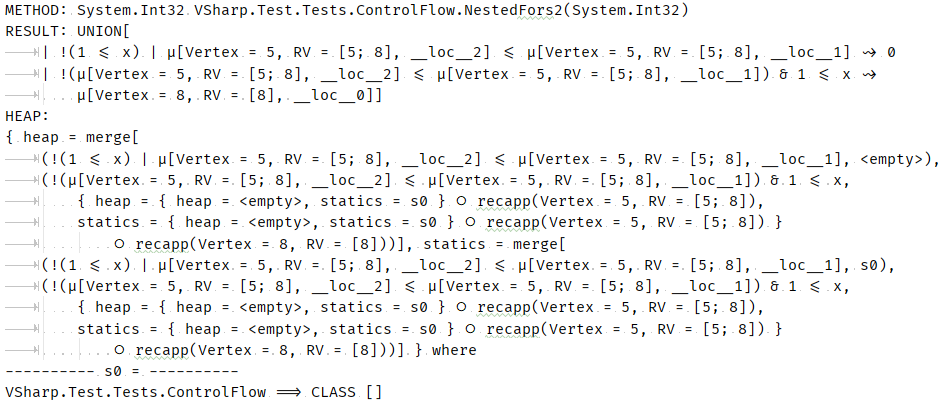
\includegraphics[scale=0.5]{Batoev/images/results.PNG}
\caption{Результат символьного исполнения метода~\ref{example:fors}}
\end{figure}

\begin{table}[t]
    \centering
    \begin{tabular}{ |p{3cm}||p{2cm}|p{2cm}|p{2cm}|  }
        \hline
        \multicolumn{4}{|c|}{Количественные характеристики тестов} \\
        \hline
        Название тестового набора &Количество тестов в наборе&Количество успешно пройденных тестов&Количество инструкций CIL\\
        \hline
        Arithmetics   &80    &77    &1968\\
        Logics        &75    &75    &1458\\
        Conditional   &10    &6     &943\\
        Recursive     &5     &5     &751\\
        Lambdas       &2     &2     &404\\
        Generic       &14    &14    &194\\
        Strings       &15    &15    &219\\
        Unsafe        &16    &16    &312\\
        Typecast      &19    &19    &969\\
        Methods       &10    &10    &238\\
        Lists         &9     &9     &1420\\
        Chess.NET     &1     &1     &2723\\
        \hline
        Всего         &256   &249   &11599\\
        \hline
    \end{tabular}
    \captionof{table}{Результаты тестирования}
    \label{experiments}
\end{table}


\FloatBarrier

\subsection{Тестирование интерпретатора}
Тестирование нового интерпретатора проводилось на тестовой подсистеме проекта <<VSharp.Test>> и на библиотеке \textsc{Chess.NET}.
Подсистема содержит тестовые наборы, затрагивающие различные конструкции и возможности языка C\#:
арифметику, логические операции,
работу с массивами разных размерностей, генерирование исключений, тесты на классы и структуры, включающие взаимодействие со статическими членами и вызовы виртуальных методов,
тесты с неограниченной рекурсией, тесты с \emph{unsafe}-кодом, тесты со строками. 

Таблица~\ref{experiments} показывает результаты проведенного тестирования. 
В наборах тестах с арифметикой и условными конструкциями была часть тестов с генерацией исключений. 
Поскольку схема обработки исключений для языка CIL не была реализована, то данные тесты были некорректно исполнены.
По той же причине не было проведено тестирования на тестовым наборе <<TryCatch>>, 
основное предназначение которого --- инициирование и перехват исключений.

\section{Заключение}

В данной работе описан подход к композициональному символьному исполнению без раскрутки. Была предложена концепция композициональной памяти с символьной адресацией. Был доказан некоторый набор свойств КСП, дающий основание для подхода в стиле систем переписывания, где символьные кучи могут сами выступать как символы. Это даёт возможность автоматически порождать уравнения на состояния, решения которых в точности отражают поведения функций, работающих с динамической памятью. Было показано как свести задачу решения уравнений на состояния к задаче проверки безопасности чистых функций второго порядка.

Данная работа нацелена на теоретические основания композиционального анализа динамической памяти. Мы оставляем апробацию этого подхода на будущее. Другим направлением будущих исследований может быть расширение нашего формализма на композициональный анализ параллельных программ.

\bibliographystyle{ugost2008ls}
\begin{thebibliography}{10}

\bibitem{baldoni2018survey}
Roberto Baldoni, Emilio Coppa, Daniele~Cono D’elia, Camil Demetrescu, and
  Irene Finocchi.
\newblock A survey of symbolic execution techniques.
\newblock {\em ACM Computing Surveys (CSUR)}, 51(3):50, 2018.

\bibitem{godefroid2007compositional}
Patrice Godefroid.
\newblock Compositional dynamic test generation.
\newblock In {\em ACM Sigplan Notices}, volume~42, pages 47--54. ACM, 2007.

\bibitem{jaffar2012tracer}
Joxan Jaffar, Vijayaraghavan Murali, Jorge~A Navas, and Andrew~E Santosa.
\newblock Tracer: A symbolic execution tool for verification.
\newblock In {\em International Conference on Computer Aided Verification},
  pages 758--766. Springer, 2012.

\bibitem{king1976symbolic}
James~C King.
\newblock Symbolic execution and program testing.
\newblock {\em Communications of the ACM}, 19(7):385--394, 1976.

\bibitem{kuznetsov2012efficient}
Volodymyr Kuznetsov, Johannes Kinder, Stefan Bucur, and George Candea.
\newblock Efficient state merging in symbolic execution.
\newblock {\em Acm Sigplan Notices}, 47(6):193--204, 2012.

\bibitem{mcmillan2010lazy}
Kenneth~L McMillan.
\newblock Lazy annotation for program testing and verification.
\newblock In {\em International Conference on Computer Aided Verification},
  pages 104--118. Springer, 2010.

\bibitem{kostyukov2018csewu}
Юрий~Олегович Костюков.
\newblock {\em Кучи как чистые функции:
  композициональное символьное исполнение
  без раскрутки}, pages 288--346.
\newblock 6. 2018.

\end{thebibliography}

\title{Композициональное символьное исполнение CIL-кода}

\titlerunning{Композициональное символьное исполнение CIL-кода}

\author{Батоев Константин Аланович}

\authorrunning{К.~А.~ Батоев}

\tocauthor{Константин Батоев}
\institute{St Petersburg State University\\
	\email{konstantin.batoev@gmail.com}}

\maketitle

% \renewcommand{\ttdefault}{cmtt}

\newsavebox\CBox
\newcommand\hcancel[2][0.1pt]{%
  \ifmmode\sbox\CBox{$#2$}\else\sbox\CBox{#2}\fi%
  \makebox[0pt][l]{\usebox\CBox}%
  \textcolor{red}{\rule[0.3\ht\CBox-#1/2]{\wd\CBox}{#1}}}

\captionsetup[figure]{name=Рисунок}

% \newtheorem*{proof}{Доказательство}

\renewcommand{\defnautorefname}{опр.}
\renewcommand{\lemautorefname}{лемм.}
\renewcommand{\remkautorefname}{зам.}
\renewcommand{\propautorefname}{св.}
\renewcommand{\exmpautorefname}{пр.}
\renewcommand{\thmautorefname}{теор.}
% \renewcommand{\crlrautorefname}{Corollary}
\renewcommand{\sectionautorefname}{разд.}
\newcommand{\algorithmautorefname}{лист.}
\newcommand{\algorithmcfname}{Листинг}
\makeatletter
\renewcommand{\ALG@name}{Листинг}
\makeatother

\algrenewcommand\alglinenumber[1]{\tiny #1:}

\lstdefinelanguage{Demo}
{
 morecomment = [l]{//}, 
 sensitive = true,
 morekeywords = {type, new, null,
   bool, int, write, read,
   fail, nop, let, alloc, in,
   if, then, else, call,
   true, false, and, or, not}
}

\definecolor{commentgreen}{RGB}{0,200,100}
\lstdefinestyle{demolang}{language=Demo,
    rulecolor=\color{blue!80!black},
    basicstyle=\ttfamily\footnotesize,
    keywordstyle=\color{blue}\ttfamily,
    stringstyle=\color{red}\ttfamily,
    commentstyle=\color{commentgreen}\ttfamily,
    numbers=left,
    numbersep=5pt,
    numberstyle=\tiny\color{black},
    escapechar=@,
    tabsize=2
}

\usemintedstyle{vs}

\counterwithin{lstlisting}{section}
\counterwithin{algocf}{section}

\fontfamily{times}
% \fontsize{10pt}{30pt}
\selectfont
\setlength{\parindent}{0em}
% \setlength{\parskip}{1em}
\renewcommand{\baselinestretch}{1.0}

\SetupFloatingEnvironment{listing}{name=Листинг}
\providecommand*{\listingautorefname}{лист.}
\renewcommand*{\figureautorefname}{рис.}
\renewcommand*{\tableautorefname}{табл.}
\SetAlgorithmName{Листинг}{лист.} 

\theoremstyle{plain}
\newtheorem{thm}{Теорема}%[section]
\newtheorem{lem}{Лемма}%[section]
% \newtheorem{crlr}{Corollary}%[section]

\theoremstyle{definition}
\newtheorem{defn}{Определение}
\newtheorem{remk}{Замечание}
\newtheorem*{remk*}{Замечание}
\newtheorem{prop}{Утверждение}
\newtheorem{exmp}{Пример}
% \newtheorem*{proof}{Доказательство}

% \newcommand{\defnautorefname}{опр.}
\newcommand{\lemautorefname}{лем.}
\newcommand{\remkautorefname}{зам.}
\newcommand{\propautorefname}{утв.}
\newcommand{\exmpautorefname}{пример}
\newcommand{\thmautorefname}{теор.}
% \renewcommand{\crlrautorefname}{Corollary}
\renewcommand{\sectionautorefname}{секция}
% \renewcommand{\algorithmautorefname}{Алгоритм}
% \renewcommand{\algorithmcfname}{Алгоритм}

% \renewcommand*{\Authsep}{\authorcr}
% \renewcommand*{\Authand}{\authorcr}
% \renewcommand*{\Authands}{\authorcr}

% \makeatletter
% \makeatother

\lstdefinelanguage{Demo}
{
 morecomment = [l]{//}, 
 sensitive = true,
 morekeywords = {new, null,
   fail, goto, halt,
   true, false, and, or, not}
}

\definecolor{commentgreen}{RGB}{0,200,100}
\lstdefinestyle{demolang}{language=Demo,
    rulecolor=\color{blue!80!black},
    basicstyle=\ttfamily\footnotesize,
    keywordstyle=\color{blue}\ttfamily,
    stringstyle=\color{red}\ttfamily,
    commentstyle=\color{commentgreen}\ttfamily,
    numbers=left,
    numbersep=5pt,
    numberstyle=\tiny\color{black},
    escapechar=@,
    tabsize=2
}

%%% For graph drawing
\definecolor {processblue}{cmyk}{0.96,0,0,0}
\definecolor {processgreen}{cmyk}{1,0,1,0}
\definecolor {processred}{cmyk}{0, 0.84, 0.80, 0.19}
\definecolor {processyellow}{cmyk}{0, 0, 1, 0}


%\newcommand{\csharp}[1]{\mintinline{csharp}{#1}}

\newcommand{\pex}{\textsc{Pex}}
\newcommand{\predator}{\textsc{Predator}}
\newcommand{\dotnet}{\textsc{.NET}}
\newcommand{\clang}{\textsc{C}}
\newcommand{\vsharp}{\textsc{V\#}}

\newcommand\addrset{loc}
\newcommand\termset{term}
\newcommand\guardset{guard}

\newcommand\eqby[1]{\mathrel{\stackrel{\mbox{\normalfont\tiny #1}}{=}}}
\newcommand\eqdef{\eqby{def}}

\newcommand\aite{ite}
\newcommand\ite[3]{\aite(#1,#2,#3)}
\newcommand\Ite[3]{\aite\big(#1,#2,#3\big)}
\newcommand\pair[2]{\langle#1, #2\rangle}
\newcommand\paiR[2]{\big\langle#1, #2\big\rangle}
\newcommand\mg[2]{#1=#2}
\newcommand\nmg[2]{#1\neq#2}
\newcommand\li[1]{LI(#1)}
\let\emptyheap\varepsilon
\newcommand\agrec{Rec}
\newcommand\agmerge{Merge}
\newcommand\agcompose{\bigcirc}
\newcommand\GRec[1]{\agrec\big(#1\big)}
\newcommand\GMerge[1]{\agmerge\big(#1\big)}
\newcommand\GCompose[2]{#1\agcompose#2}
\newcommand\agho{App}
\newcommand\gapp[1]{\agho(#1)}
\newcommand\GApp[1]{\agho\big(#1\big)}
\newcommand\aunion{\texttt{UNION}}
\newcommand\union[1]{\aunion\big(#1\big)}
\newcommand\Union[1]{\aunion\Big(#1\Big)}
\newcommand\aderef{readStore}
\newcommand\readTerm{readTerm}
\newcommand\writeTerm{writeTerm}
\newcommand\afind{find}
\newcommand\find[5]{\afind(#1,#2,#3,#4,#5)}
\newcommand\finD[5]{\afind\big(#1,#2,#3,#4,#5\big)}
\newcommand\Find[5]{\afind\Big(#1,#2,#3,#4,#5\Big)}
\newcommand\deref[2]{\aderef(#1,#2)}
\newcommand\Deref[2]{\aderef\big(#1,#2\big)}
\newcommand\compose[2]{#1\circ#2}
\newcommand\lmbd[2]{\lambda #1.#2}
\newcommand\lmbdx[1]{\lambda x.#1}
\newcommand\dom[1]{dom(#1)}
\newcommand\Dom[1]{dom\big(#1\big)}

\newcommand\Li[1]{LI\big(#1\big)}
\newcommand\amutate{writeStore}
\newcommand\amutateStack{writeStack}
\newcommand\mutate[3]{\amutate(#1,#2,#3)}
\newcommand\mutateStack[4]{\amutateStack(#1,#2,#3,#4)}
\newcommand\rdbodyext[6]{\Union{\big\{\paiR{#4\mg{#1}{#5}}{#6\big(#2(#5), xs\big)} \mid #5\in\dom{#2} \big\}\\&\qquad\qquad\qquad\cup\paiR{#4\bigwedge_{\mathclap{#5\in\dom{#2}}}{\nmg{#1}{#5}}}{#6\big(#3, xs\big)}}}
\newcommand\rdbody[4]{\rdbodyext{#1}{#2}{#3}{}{l}{#4}}
\newcommand\wrtbody[6]{\Union{&\paiR{\mg{#1}{#2}}{\writeTerm\big(#3,#4,#6\big)},
    \\&\paiR{\nmg{#1}{#2}}{\writeTerm\big(#5(#1),#4,#6\big)}}}
\newcommand{\var}[1]{\mathit{#1}}


\begin{abstract}
Известно, что наибольшую сложность в области верификации программ представляет задача доказательства корректности программ с циклическими участками кода. Опираясь на подход символьного исполнения программ и на введенные формализмы обобщённых куч в работе~\cite{kostyukov2018csewu}, данная работа представляет алгоритм композиционального символьного исполнения без раскрутки отношения перехода программ с произвольным графом потока управления. На его основе был реализован символьный интерпретатор языка CIL в проекте V\#, символьной виртуальной машине для анализа .NET. Была проведена апробация алгоритма на примерах, включающих сложные потоки управления, и интерпретатора на тестовой базе проекта VSharp.Test и на библиотеке Chess.NET.
\end{abstract}
\section*{Введение}
Поиск путей в графе с ограничением в виде формальных языков~\cite{FLCpathProblem} --- это задача, в которой формальные языки используются для задания множества искомых путей. В таком подходе каждый путь соответствует слову, состоящему из меток его рёбер, а ограничением на путь является принадлежность соответствующего ему слова некоторому заданному формальному языку.

В качестве класса формальных языков по иерархии Хомского наибольший интерес представляют контекстно-свободные языки. В отличие от регулярных они обладают большей выразительностью. Поэтому в задаче поиска путей контекстно-свободные ограничения позволяют задавать более сложные отношения между вершинами. Так, например, важный класс запросов поиска вершин, лежащих на одном уровне иерархии~\cite{zhlang-2016}, задаётся только контекстно-свободными, но не регулярными ограничениями. Запросы такого вида, как и другие запросы с контекстно-свободными ограничениями имеют широкое применение в биоинформатике~\cite{bio-application} и при обработке rdf-файлов~\cite{zhlang-2016}.

Наиболее удобным и подходящим инструментом для работы с граф\-структурированными данными являются графовые базы данных. Так же как и реляционные, графовые базы данных поддерживают свой язык запросов. С его помощью графовые базы данных позволяют решать вышеупомянутую задачу поиска путей. Но ограничения на пути, которые поддерживается в наиболее распространённых базах данных, являются в лучшем случае регулярными.

Отсутствие поддержки контекстно-свободных ограничений в графовых базах данных, во-первых, сильно ограничивает выразительность языка запросов. Во-вторых, при необходимости в более сложных запросах разработчикам приходится самим писать алгоритмы, решающие задачу контекстно-свободной достижимости для их частного случая. Так, например, Хуэй Мяо и др.~\cite{datascince-lifecycle} разработали систему хранения и отслеживания версий артефактов, возникающих при научных работах. Вся информация про артефакты хранилась в графовой базе данных. При этом при разработке возникла потребность в выполнении запросов с контекстно-свободными ограничениями для выявления взаимоотношений между различными версиями различных артефактов. Это и послужило началом статьи~\cite{datascince-lifecycle}, в которой приводятся алгоритмы решения частных запросов.

В недавнем исследовании Йохем Куйперс и др.~\cite{Kuijpers:2019:ESC:3335783.3335791} произвели сравнительный анализ наиболее известных алгоритмов поиска путей с конте\-кстно-свободными ограничениями. Алгоритмы запускались на графах, находящихся в хранилище графовой базы данных Neo4j. По результатам исследования было показано, что в контексте Neo4j алгоритмы обладают большим временем работы, и поэтому дальнейшая работа по расширению языка запросов прекратилась. При этом Рустам Азимов~\cite{Azimov:2018:CPQ:3210259.3210264} предоставил матричный алгоритм и его реализацию, которая работает за разумное время на реальных данных. Но, так как алгоритм был реализован вне контекста базы данных, его результат приняли недостаточно показательным. Поэтому вопрос о реализуемости запросов с контекстно-свободными ограничениями в графовых базах данных, а соответственно и о возможности расширения языка запросов для их поддержки остаётся открытым.

\section{Постановка задачи}
Целью данной работы является полная поддержка запросов с конте\-кстно-свободными ограничениями для графовой базы данных. А именно, необходимо предоставить пользователю возможность формулировать запросы с контекстно-свободными ограничениями в терминах одного из существующих стандартных языков запросов и исполнять их в графовой базе данных за приемлемое время. Для достижения этой цели были поставлены следующие задачи.

\begin{itemize}
    \item Выполнить обзор существующих реализаций поддержки запросов с контекстно-свободными ограничениями в графовых базах данных. В результате обзора необходимо выбрать наиболее перспективный с точки зрения производительности алгоритм решения задачи контекстно-свободной достижимости и подходящую для его интеграции базу данных. При выборе базы данных необходимо учитывать как возможность интеграции выбранного алгоритма, так и возможность поддержки одного из стандартных языков запросов, позволяющего выражать контекстно-свободные ограничения.
    \item Интегрировать выбранный на предыдущем шаге алгоритм в выбранную графовую базу данных.
    \item Расширить язык запросов выбранной базы данных конструкциями, необходимыми для выражения контекстно-свободных ограничений.
    \item Произвести замеры производительности полученного решения и сравнить его с существующими решениями.
\end{itemize}


\section{Обзор}

\subsection{Терминология}
Контекстно-свободной грамматикой называется $G = (\Sigma, N, P, S)$, где $\Sigma$ --- алфавит терминальных символов, $N$ --- алфавит нетерминальных символов, $P$ --- множество правил вида $A \rightarrow \alpha$, где $A \in N$, $\alpha \in (\Sigma \cup N)^*$, а $S \in N$ --- выделенный стартовый нетерминал.

% \gsv{про S забыли}.

Языком $L$ над алфавитом $\Sigma$ называется любое подмножество $2^{\Sigma^*}$. Языком, порождаемой грамматикой G, является множество $L(G) = \{S \xRightarrow{*} \beta, \beta \in \Sigma^*\}$, где $S \xRightarrow{*} \beta$ означает, что из нетереминала $S$ путём последовательного применения правил грамматики выводится $\beta$.

Контекстно-свободная грамматика $G = (\Sigma, N, P, S)$ находится в осла\-бленной нормальной форме Хомского, если любое её правило имеет вид $A \rightarrow BC$, где $A, B, C \in N$, либо $A \rightarrow a$, где $A \in N, a \in \Sigma$. В отличие от нормальной формы Хомского в ослабленной, во-первых, допускается присутствие стартового нетерминала $S$ в правых частях правил грамматики, во-вторых, запрещаются правила вида $S \rightarrow \epsilon$, где $\epsilon$ --- пустая строка.

% \gsv{Это не нормальная форма Хомского. У НФХ есть дополнительные ограничения. Мы называем то, что здесь, ослабленной НФХ. Важно отдельно проговорить разницу с НФХ.}

В задаче поиска путей с ограничениями в виде формальных языков дан граф $(V, E)$, разметка его рёбер $l: E \rightarrow \Sigma$ и язык $L$ над алфавитом $\Sigma$. Требуется найти множество всех пар вершин, между которыми существует путь, метки на рёбрах которого образуют слово в заданном языке. То есть требуется найти следующее множество:
\[\{(v, to): \exists p=(e_1,...,e_n) \in E^*: l(e_1)...l(e_n) \in L,~src(e_1)=v,~dst(e_n)=to\}\]
Здесь $src(e)$ и $dst(e)$ для $e \in E$ означают начальную и конечную вершину ребра $e$. В данном контексте язык $L$ называется языком ограничений.
% \gsv{У Вас вершины v и to никак с путём не связаны}

Задача поиска путей с контекстно-свободными ограничениями --- это задача поиска путей в виде формальных языков, в которой язык задаётся контекстно-свободной грамматикой.

\subsection{Графовые базы данных}
Графовые СУБД\footnote{СУБД --- Система управления базами данных} (далее просто графовые базы данных) --- это разновидность СУБД, в которой данные хранятся в виде графов. В отличие от других разновидностей, в графовых базах данных отношения между объектами так же важны, как и сами объекты.

Основной моделью представления графов в таких базах данных является gpraph property model~\cite{graph-propery-model}. В ней каждая сущность может содержать набор свойств в формате ключ-значение. Основными сущностями являются узлы и отношения. Узлы соответствуют вершинам графа и помимо свойств могут иметь несколько меток. Отношения соответствуют рёбрам и имеют ровно одну метку, которая называется типом отношения. На рисунке~\ref{fig:graph_bd_1} показан небольшой пример графа в такой модели. 

\begin{figure}[h]
\centering
    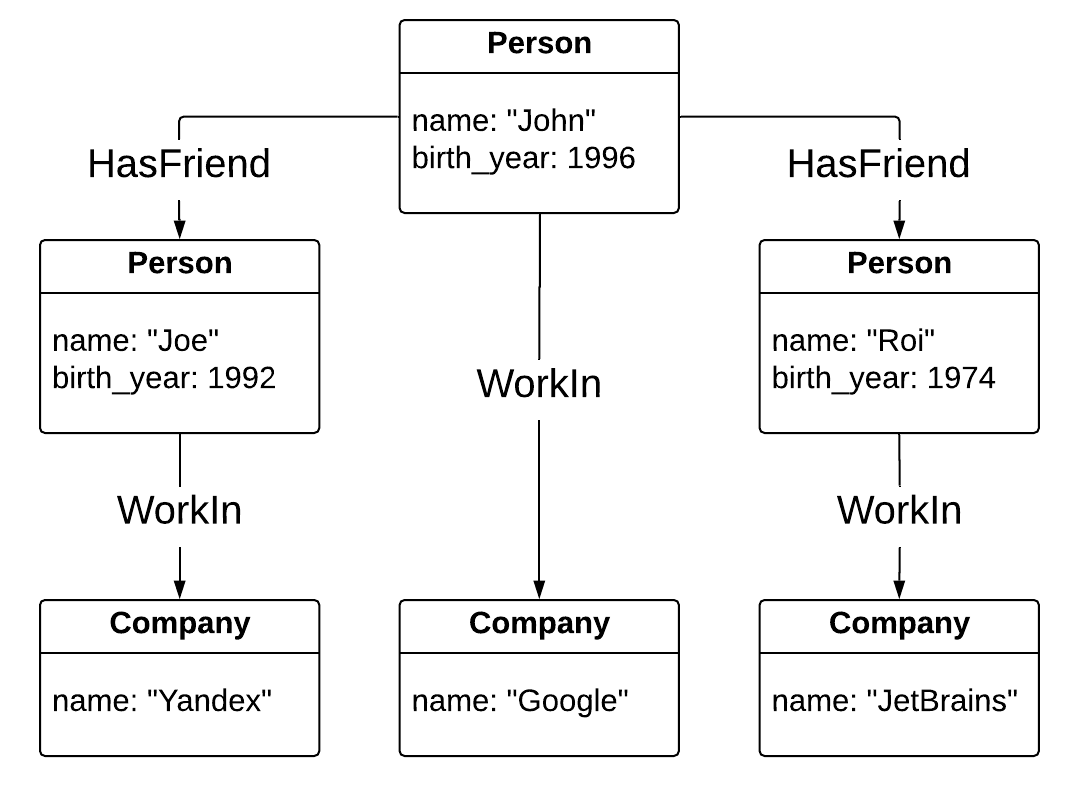
\includegraphics[width=0.7\linewidth]{Terekhov/pictures/graph_bd_1.png}
    \caption{Пример социального графа}
    \label{fig:graph_bd_1}
\end{figure}

Для работы с графами графовые базы данных предоставляют язык запросов, самым популярным из которых является Cypher~\cite{cypher-language}. В нём главный интерес представляют запросы вида сопоставления с образцом. Они позволяют задавать интересующие пути или подграфы в виде шаблонов и описывать информацию, которую нужно извлечь после удачного сопоставления. На рисунке~\ref{code:cypher_query} приведён пример такого запроса. Шаблон пути описывается в выражении MATCH. В нём между круглыми скобками задаются шаблоны вершин, а между квадратными шаблоны рёбер. Таким образом в данном примере задаются следующие ограничения: путь должен начинаться из вершины с меткой Person и именем John и состоять из двух рёбер, первое из которых должно иметь тип HasFriend, а второе WorkIn. В выражении RETURN задаётся информация, которую нужно извлечь. В данном примере это имя последней в пути вершины. В итоге ответом на такой запрос являются имена компаний, в которых работают друзья Джона. Результатом работы этого запроса на графе из рисунка~\ref{fig:graph_bd_1} является множество \{"Yandex", "JetBrains"\}.

%\lstset{
%   basicstyle=\fontsize{14}{14}\selectfont\ttfamily
%}

\begin{figure}[h]
\begin{lstlisting}[language=sql]
MATCH (p:Person)-[:HasFriend]->()-[:WorkIn]->(to)
WHERE p.name = "John"
RETURN to.name
\end{lstlisting}
\caption{Пример конечного запроса на языке Cypher}
\label{code:cypher_query}
\end{figure}

С формальной точки зрения шаблоны пути в выражении MATCH позволяют поставить задачу поиска путей с ограничениями в виде формальных языков. Так в запросе на рисунке~\ref{code:cypher_query} языком ограничений является конечный язык $\{(HasFriend, WorkIn)\}$. Для запроса на рисунке~\ref{code:cypher_query_2} ограничением является регулярный язык $\{A, B\}^*$. 

\begin{figure}[h]
\begin{lstlisting}[language=sql]
MATCH (v)-[:A | :B *]->(to)
RETURN to.name
\end{lstlisting}
\caption{Пример регулярного запроса на языке Cypher}
\label{code:cypher_query_2}
\end{figure}

При этом регулярные ограничения поддерживаются лишь частично и позволяют искать только пути произвольной длины с заданными метками на рёбрах, а более глубокие регулярные выражения не поддерживаются. Поэтому на текущий момент язык запросов довольно ограничен.

\subsection{Существующие решения}
Как было упомянуто раннее, ни одна графовая база данных не поддерживает запросов с контекстно-свободными ограничениями. Тем не менее существуют альтернативные решения поддержки таких запросов. 

\subsubsection{Парсер-комбинаторы для Neo4j}\label{sec:pareser-combinators}
В 2018 году группой исследователей из JetBrains Research на основе библиотеки Meerkat была разработана библиотека для поддержки запросов с контекстно-свободными ограничениями~\cite{parser-combinators}. Она использует графовую базу данных Neo4j~\cite{neo4j} как хранилище графов и позволяет задавать запросы в виде парсер-комбинаторов. Основным достоинством данной работы является то, что с помощью этой библиотеки кроме контекстно-свободных запросов можно выразить базовую часть языка Cypher. Но так как конкурировать с оригинальной реализацией выполнения запросов Neo4j очень сложно, это достигается вместе c сильной потерей производительности. Кроме этого контекстно-свободные запросы обрабатываются также достаточно медленно.

Таким образом данное решение является альтернативой языка запросов Neo4j, а не его расширением. Из-за медленного времени работы такое решение подходит только для работы с небольшими графами. 

\subsubsection{Расширение языка запросов SPARQL}\label{subsection:cypher-extention-2}
%Про sparql%
В 2016 Сяованг Чжан предоставил язык cfSPARQL~\cite{zhlang-2016} --- расширение языка SPARQL, который способен выразить запросы с контекстно-свободными ограничениями. Также он привёл алгоритм для вычисления таких запросов и замеры производительности. Но, во-первых, работа была сделана вне контекста графовой базы данных, а во-вторых, время работы предложенного алгоритма было больше, чем время работы парсер-комбинаторов.

\subsubsection{Существующие реализации алгоритмов решения задачи контекстно-свободной достижимости}
Основной сложностью расширения языка запросов для поддержки запросов с контекстно-свободными ограничениями является долгое время работы соответствующих алгоритмов. Так, например, в 2019 году Йохем Куйперс и другие исследователи с целью попытки расширения языка запросов Cypher для графовой базы данных Neo4j произвели сравнительный анализ производительности наиболее известных алгоритмов решения задачи контекстно-свободной достижимости.

В данном исследовании были рассмотрены и произведены замеры времени работы алгоритма Элле Хелингса~\cite{hellings-2015}, основанного на атрибутных грамматиках, восходящего алгоритма Фреда Сантоса~\cite{santos-2018}, матричного алгоритма Рустама Азимова~\cite{Azimov:2018:CPQ:3210259.3210264} и алгоритма Петтери Севона~\cite{bio-application}. Все алгоритмы были интегрированы в Neo4j и запускались на графах, находящихся в её хранилище. Алгоритмы были написаны на языке Java, при этом их реализация являлась однопоточной.

% \gsv{В таких местах надо сразу ссылку на алгоритм давать.}

По результатам замеров производительности было показано, что время работы алгоритмов является слишком большим и неприемлемым для широкого практического использования. Поэтому дальнейшая работа по интеграции и расширению языка запросов была приостановлена.

Тем не менее, матричный алгоритм Рустама Азимова в сравнительном анализе Йохема Куйперса был реализован без необходимых матричных библиотек, которые могут сильно уменьшить время его работы. Так, например, в исследовании Никиты Мишина и др.~\cite{azimov-evalution} был произведён сравнительный анализ времени работы нескольких реализаций алгоритма Рустама Азимова, основанных на различных специализированных матричных библиотеках. Графы и запросы к ним были взяты из объемлющего набора данных CFPQ\_Data~\cite{cfpq-data}, предоставленного лабораторией языковых инструментов JetBrains Research. 

Результаты замеров Никиты Мишина и др. показали, что при грамотной реализации алгоритма Рустама Азимова и использовании подходящих матричных библиотек можно добиться очень высокой производительности. Поэтому, так как основной проблемой применимости запросов с контекстно-свободными ограничениями является долгое время работы соответствующих алгоритмов, в качестве алгоритма решения задачи конте\-кстно-свободной достижимости был выбран матричный алгоритм Рустама Азимова.

\subsection{Матричный алгоритм Рустама Азимова}\label{sec:matrix-algo}
Выбранный в предыдущей главе алгоритм Рустама Азимова~\cite{Azimov:2018:CPQ:3210259.3210264}, в отличие от других алгоритмов решения задачи контекстно-свободной достижимости~\cite{hellings-2015, santos-2018, zhlang-2016}, работает с графами в виде разреженных матриц смежности. Данный алгоритм состоит из последовательности операций над разреженными матрицами, время работы которых зависит не от размеров матричных операндов, а от количества их ненулевых элементов.

На вход алгоритму (см. алгоритм 1) поступает помеченный граф $D=(V,E)$ и контекстно-свободная грамматика $G=(\Sigma, N, P, S)$ в ослабленной нормальной форме Хомского. Для каждого нетерминала $A$ в ассоциативном массиве $T$ хранится соответствующая ему булева матрица $T[A]$. На всём этапе алгоритма поддерживается следующий инвариант: $T[A]_{i,j} = 1$ равносильно существует пути, метки на рёбрах которого образуют слово, выводящееся из нетерминала $A$. На первом этапе происходит инициализация матриц с помощью простых правил грамматики, после чего инвариант выполняется для всех путей единичной длины. На втором этапе происходит транзитивное замыкание, после чего этот инвариант верен для всех путей. Результатом данного алгоритма является матрица, соответствующая стартовому нетерминалу $S$.

%  Это позволяет для его реализации использовать многопоточные матричные библиотеки, с помощью которых можно добиться очень высокой производительности. Поэтому на текущий момент алгоритм Рустама Азимова показывает наилучшее время работы на практике.

\begin{algorithm}
\caption{Матричный алгоритм Рустама Азимова}

\begin{algorithmic}[1]
\Function{contextFreePathQuerying}{$D$, $G$}
    \State{$n =$ getNodeCount(D)}
    \State{$N =$ getAllNonterms(G)}
    \State{$E =$ getEdges($D$)}
    \State{$P =$ getRules($G$)}
    \State{$S =$ getStartNonterm($G$)}
    \State{$T = \{A \rightarrow \varnothing_{n \times n} : A \in$ $N$ \} }
    \ForAll{$(v, to, label) \in E$}
    \Comment{Инициализация матриц}
        \ForAll{$A \rightarrow label \in P$}
            \State{$T[A]_{i,j} = 1$}
        \EndFor
    \EndFor    
    \While{$\exists A: T[A]$ is changing}
    \Comment{Вычисление замыкания}
        \ForAll{$A \rightarrow BC \in P$}
            \State{$T[A] \oplus= T[B] \otimes T[C]$}
        \EndFor
    \EndWhile
\State \Return $T[S]$
\EndFunction

\end{algorithmic}
\end{algorithm}

Практическое время работы алгоритма Рустама Азимова сильно зависит от производительности используемой матричной библиотеки. Это накладывает некоторые ограничения на выбор подходящей графовой базы данных, так же как и возможность представления графов в матричном виде.

\subsection{RedisGraph}
RedisGraph~\cite{redis-graph} --- это высокопроизводительная графовая база данных, поддерживающая язык запросов Cypher. В отличие от наиболее распространённой графовой базы данных Neo4j~\cite{neo4j}, RedisGraph написан на языке Си и для работы с данными использует Redis~\cite{redis}, основным достоинством которого является возможность хранить данные прямо в оперативной памяти. Это позволяет RedisGraph быстро обрабатывать пользовательские запросы.

Также RedisGraph является единственной графовой базой данных, которая работает с графами в виде разреженных матриц смежности и транслирует запросы языка Cypher в матричные выражения. Для представления графов в таком виде и работы с ними в терминах линейной алгебры используется мощный матричный фреймворк GraphBlas~\cite{graph-blas}. Его реализация SuiteSparse~\cite{suite-sparse} является многопоточной и сильно оптимизирована, что позволяет RedisGraph добиться высокой производительности.

Из всего этого следует, что RedisGraph идеально подходит для интеграции матричного алгоритма. Во-первых, графы представляются в необходимом алгоритму виде, что позволит избежать издержек на конвертацию форматов. Во-вторых, использование SuiteSparse для вычисления матричных операций позволит добиться высокой производительности. Поэтому RedisGraph был выбран в качестве графовой базы данных для интеграции матричного алгоритма и расширения языка запросов.

% Так как алгоритм Рустама Азимова работает с матричным представлением графа,, как наиболее подходящий для интеграции матричного алгоритма.

\subsection{Расширение языка Cypher}\label{subsection:cypher-extention}
На текущий момент оригинальная версия языка Cypher, используемая в том числе и в RedisGraph, не поддерживает запросов с контекстно-свободными ограничениями. Но тем не менее в 2017 году был разработан черновой вариант спецификации расширения Cypher~\cite{cypher-specification}, которая вводит в язык шаблоны путей. Они позволяют выразить более сложные запросы, в том числе запросы с контекстно-свободными ограничениями.

Шаблоны путей являются альтернативой шаблонам рёбер, которые есть в оригинальном Cypher. Они, как и шаблоны рёбер, могут встречаться в выражении MATCH и иметь своё направление. Кроме этого в глобальной области запроса им можно задавать имя, на которое потом можно ссылаться внутри других шаблонов.

Шаблон пути представляет из себя регулярное выражение над некоторыми примитивами. В качестве таких примитивов могут выступать шаблоны рёбер, шаблоны вершин и ссылки на именованные шаблоны путей. Также любым подвыражениям можно задавать своё направление. Основная часть конкретного синтаксиса данного расширения приведена на рисунке~\ref{fig:cypher_syntax}.

\begin{figure}[]
\begin{align*}
\begin{split}
PathPattern     &= ["<"],~"-/",~PathExpression,~"/-",~[">"]\\
PathExpression  &= \{PathAlternative\}\\
PathAlternative &= PathRepetition,~\{"|", PathRepetition\}\\
PathRepetition  &= ["<"],~PathBase,~[">"],~("*")
\end{split}\\
\begin{split}
PathBase &= PathEdge \\
         &~~|~PathNode \\
         &~~|~PathReference \\
         &~~|~"[",~PathExpression,~"]"
\end{split}\\
\begin{split}
PathEdge      &= Label \\
PathNode      &= "(",~[Label,~\{"|",~Label\}],~")" \\
PathReference &= "\sim",~SymbolicName; \\
Label         &= ":",~LabelName
\end{split}
\end{align*}
\caption{Расширение конкретного синтаксиса Cypher}
\label{fig:cypher_syntax}
\end{figure}

Каждый шаблон пути задаёт отношение на множестве вершин. Поэтому семантикой языка шаблонов путей $L_{P}$ в контексте графа $G(V, E)$ является отображение $\llbracket \cdot \rrbracket_{G}: L_P \rightarrow V \times V$, которое каждому шаблону $p\in L_P$ сопоставляет множество пар вершин, между которыми существует путь, удовлетворяющий данному шаблону $p$. 

Подробное описание данной семантики приводится в таблице~\ref{tab:cypher_sematic}.  В ней наибольший интерес представляют именованные шаблоны путей, так как именно с помощью них можно выразить запросы с контекстно-свободными ограничениями. Все именованные шаблоны путей $S_i = p_j$ можно рассматривать как правила контекстно свободной грамматики с алфавитом нетерминалов $\{S_i\}_{i=1}^n$. Тогда каждый нетерминал $S_j$ порождает язык $L_{S_j} \subset L_p$, а семантикой соответствующего именованного шаблона пути $S_j=p_j$ является множество $\bigcup\limits_{p \in L_{s_j}} \llbracket p \rrbracket_{G}$.

На рисунке~\ref{code:cypher_query_3} приведён пример запроса в расширенном синтаксисе. В нём декларируется именованный шаблон S, который задаёт множество правильных скобочных последовательностей над ребрами с типом L и R. Далее в выражении MATCH задаётся шаблон пути, состоящий из ссылки на шаблон S. Таким образом результатом обработки запроса является множество всех пар вершин, между которыми существует путь, метки на рёбрах которого образуют правильную скобочную последовательность. 

\begin{table}[h!]
\begin{adjustbox}{max width=\textwidth}
\begin{tabular}{|c|c|c|}
\hline
$p \in L_P$                                                                                  & $\llbracket p \rrbracket_{G}$                                                                                                                                                                                   & Описание шаблона пути                                                                                                         \\ \hline
\hline
()                                                                                            & $\{(v, v): v \in V\}$                                                                                                                                                                                           & \begin{tabular}[c]{@{}c@{}}Пустой путь, состоящий из \\ одной произвольной вершины\end{tabular}                               \\ \hline
:a                                                                                            & $\{e=(v,to): e \in E, type(e)=a\}$                                                                                                                                                                              & \begin{tabular}[c]{@{}c@{}}Путь единичной длины,\\  состоящий из ребра с типом $a$\end{tabular}                               \\ \hline
(:b)                                                                                          & $\{(v, v): v \in V, label(v)=b\}$                                                                                                                                                                               & \begin{tabular}[c]{@{}c@{}}Пустой путь, состоящий из одной\\  вершины, помеченной меткой $b$\end{tabular}                     \\ \hline
$\alpha~\beta$                                                                                & $\llbracket \alpha \rrbracket_{G}\circ \llbracket \beta \rrbracket_{G}$                                                                                                                                         & Конкатенация путей $\alpha$ и $\beta$                                                                                         \\ \hline
$\alpha~|~\beta$                                                                              & $\llbracket \alpha \rrbracket_{G}\cup \llbracket \beta \rrbracket_{G}$                                                                                                                                          & Альтренатива между путями $\alpha$ и $\beta$                                                                                  \\ \hline
$[\alpha]$                                                                                    & $\llbracket \alpha \rrbracket_{G}$                                                                                                                                                                              & \begin{tabular}[c]{@{}c@{}}Квадратные скобки позволяют \\ группировать  выражения \\ для задания ассоциативности\end{tabular} \\ \hline
\textless{}$\alpha$                                                                           & $\{(to, v): (v, to) \in \llbracket \alpha \rrbracket_{G}\}$                                                                                                                                                     & Путь, обратный к пути $\alpha$                                                                                                \\ \hline
\textless{}$\alpha$\textgreater{}                                                             & $\llbracket \alpha~|~$\textless{}$\alpha \rrbracket_{G} $                                                                                                                                                       & \begin{tabular}[c]{@{}c@{}}Альтернатива между путём $\alpha$ и\\ обратным к нему\end{tabular}                                 \\ \hline
$\alpha^*$                                                                                    & $\llbracket \alpha \rrbracket_{G}^{*}$                                                                                                                                                                          & \begin{tabular}[c]{@{}c@{}}Путь, состоящий из\\ конкатенации 0 или более путей $\alpha$\end{tabular}                          \\ \hline
\begin{tabular}[c]{@{}c@{}}$\{S_i = p_i\}_{i=1}^{n}$\\ -- named\\  path patterns\end{tabular} & \begin{tabular}[c]{@{}c@{}}$P = \{S_i \rightarrow p_i\}_{i=1}^n$\\ $Gram_j = (\Sigma, \{S_i\}_{i=1}^n, P, S_j)$\\ $\llbracket S_j \rrbracket_{G} = \bigcup\limits_{p \in L(G)}{\llbracket p \rrbracket_{G}}$\end{tabular} & Именнованые шалоны путей                                                                                                      \\ \hline
$\sim$$S$                                                                                     & $\llbracket S \rrbracket_{G}$                                                                                                                                                                                   & \begin{tabular}[c]{@{}c@{}}Ссылка на именнованный\\  шаблон пути\end{tabular}                                                 \\ \hline
\end{tabular}
\end{adjustbox}
\caption{Семантика языка шаблонов путей}
\label{tab:cypher_sematic}
\end{table}

\begin{figure}[h!]
\begin{lstlisting}[language=sql]
PATH PATTERN S = ()-/ [:L ~S :R] | [~S ~S] | () /-()
MATCH (v)-/ ~S /-(to)
RETURN v, to
\end{lstlisting}
\caption{Пример запроса в расширенном синтаксисе Cypher}
\label{code:cypher_query_3}
\end{figure}

Данная спецификация расширения Cypher была представлена официальными разработчиками и сильно расширяет выразительность языка, предоставляя удобную возможность выражать запросы как с регулярными, так и с контекстно-свободными ограничениями. Поэтому в моей работе приводится поддержка выполнения запросов именно для этого расширения языка.

% \gsv{Не хватает какого-то чёткого вывода про то, что вот именно это мы и буем использовать.}

\section{Реализация}
По результатам обзора было решено реализовать поддержку расширения языка Cypher, представленную в главе~\ref{subsection:cypher-extention}, для графовой базы данных RedisGraph. За основу алгоритма, решающего задачу поиска путей с контекстно-свободными ограничениями, был взят матричный алгоритм Рустама Азимова, описанный в главе~\ref{sec:matrix-algo}.

% \gsv{И зжесь надо ещё раз подитожить в духе "по результатм обзора было решено сделать то и это с использованием того и сего"}

\subsection{План выполнения запроса}\label{execution-plan}
В RedisGraph основной частью обработки запроса является построение плана его выполнения. Её часть, которая относится к шаблонам путей приведена на рисунке~\ref{fig:execution_plan}. В ней зелёным цветом выделено то, что было добавлено или расширено.

В самом начале, после получения запроса строится его абстрактное синтаксическое дерево \textit{AST}. Далее, из него извлекаются именованные и неименованные шаблоны путей \textit{PathPattern} и \textit{NamedPathPatterns}, после чего они преобразуются в более удобное промежуточное представление \textit{PathExpr}. При этом, для дальнейшего связывания ссылок, именованные шаблоны сохраняются в глобальном контексте запроса \textit{PathPatternCtx}.

На следующем этапе происходит трансляция промежуточных представлений \textit{PathExpr} в матричные выражения \textit{AlgebraicExpression}. В них операндами являются либо матрицы, полученные из указанного в запросе графа \textit{GraphCtx}, либо ссылки на именованные шаблоны путей из \textit{PathPatternCtx}. Основной идеей трансляции является то, что после вычисления матричного выражения получается матрица, которая задаёт то же самое отношение на множестве вершин, что и исходный шаблон пути.

Далее каждое такое выражение формирует новую операцию плана выполнения запроса \textit{CfpqTraverseOp}. При её вычислении сначала происходит запуск расширенной версии матричного алгоритма Рустама Азимова. Он решает задачу контекстно-свободной достижимости, заданной именованными шаблонами путей. После этого все ссылки в матричном выражении заменяются на полученные в ходе алгоритма матрицы и происходит вычисление матричного выражения. Каждая такая операция добавляется в план выполнения запроса.

%  \gsv{Используйте \textit{CfpqTraverseOp} вместо долларов для длинных слов. Они тогда не распадаются из-а лишних пробелов.}

\begin{figure}[H]
\centering
    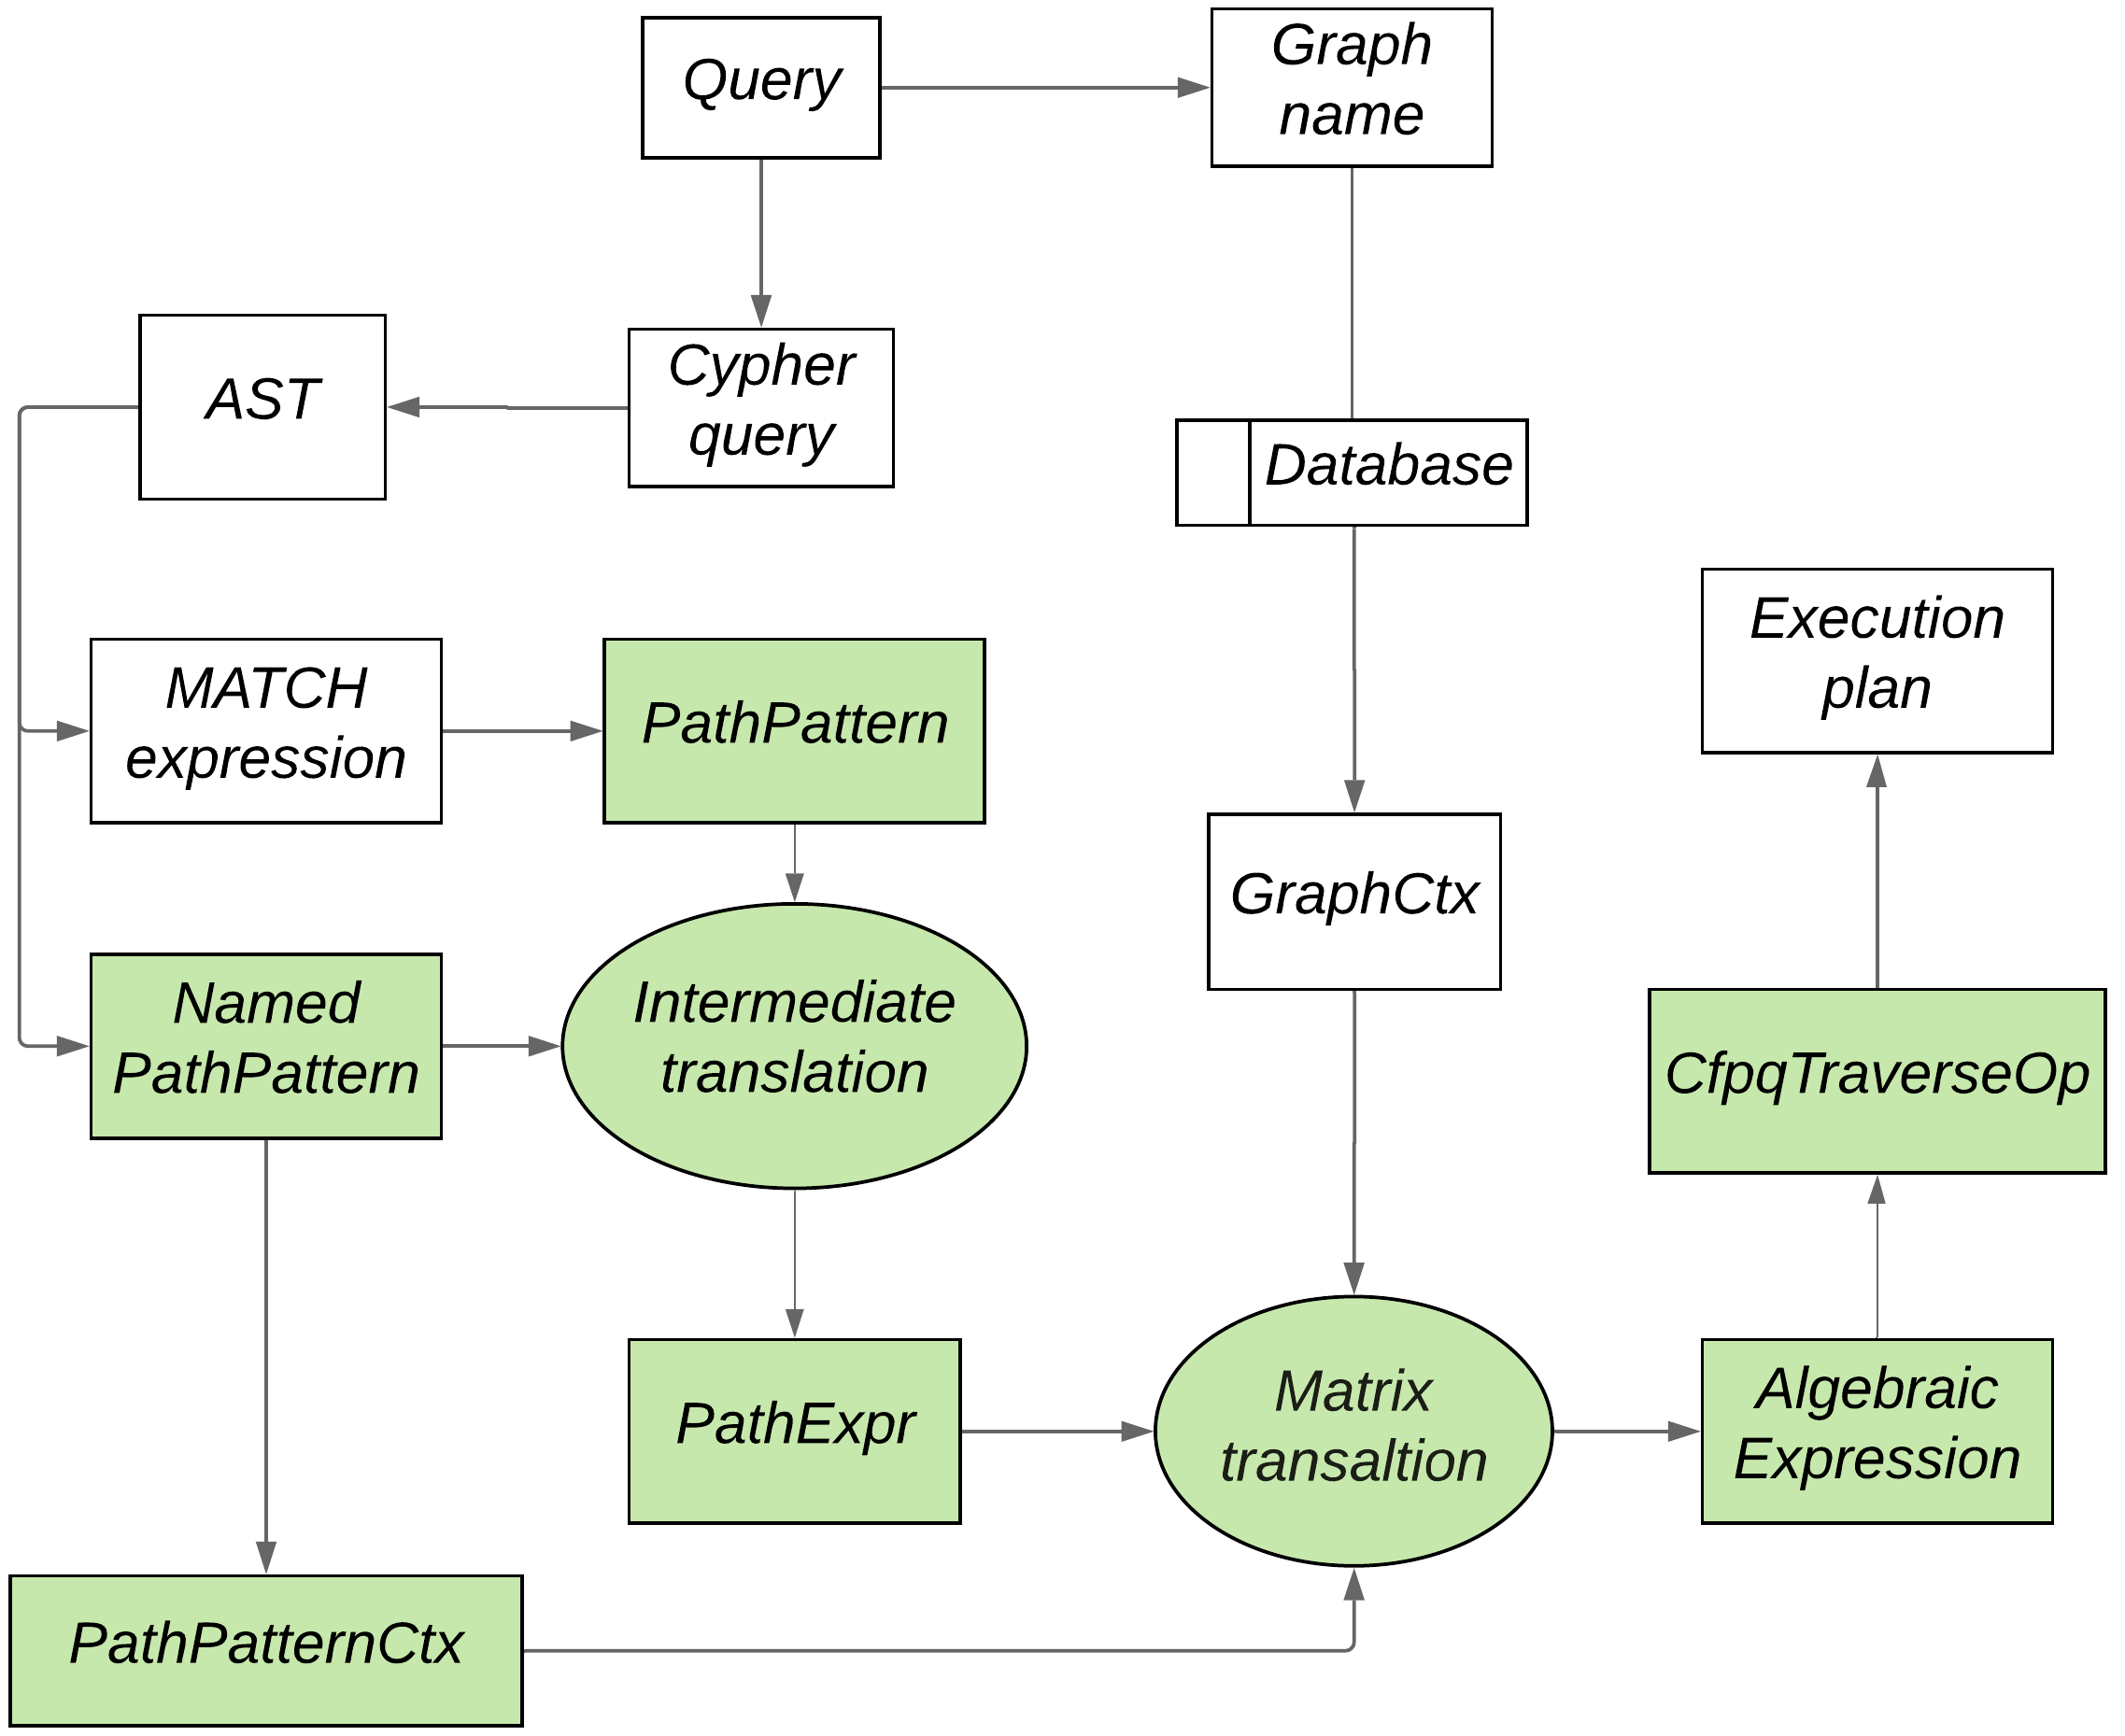
\includegraphics[width=1.0\linewidth]{Terekhov/pictures/execution_plan_3.png}
    \caption{Расширение построения плана выполнения запроса}
    \label{fig:execution_plan}
\end{figure}

\subsection{Промежуточное представление}\label{matrix-translation}
Шаблоны путей, полученные из \textit{AST}, транслируются в промежуточное представление \textit{PathExpr}. Оно позволяет задавать более простой абстрактный синтаксис, который описан на рисунке~\ref{fig:intermidiate_repr}. 

Таким образом, альтернативе и конкатенации шаблонов соответствуют \textit{PathAlt} и \textit{PathSeq}, \textit{PathGroup} позволяет задавать направление пути и наличие замыкания, а \textit{PathBasic} соответствует либо примитивным шаблонам \textit{PathNode}, \textit{PathEdge} и \textit{PathRef}, либо целому выражению \textit{PathExpr}. Примеры промежуточного представления шаблонов приведены в таблице~\ref{tab:inter_examples}.
\begin{figure}[h!]
\begin{align*}
\begin{split}
PathExpr=~ &PathSeq(PathExpr,~PathExpr)~|\\
           &PathAlt(PathExpr,~PathExpr)~|\\
           &PathGroup(PathBasic, direction, range)
\end{split}\\
\begin{split}
PathBasic=~ &PathNode(label)~|\\
            &PathEdge(type)~~|\\
            &PathRef(name) ~~|\\
            &PathExpr
\end{split}\\
\begin{split}
direction \in ~&\{inbound,~outbound,~bidirectional\}\\
range \in     ~&\{*, \varnothing\}
\end{split}
\end{align*}
\caption{Промежуточное представление PathExpr}
\label{fig:intermidiate_repr}
\end{figure}

\begin{table}[h]
\centering
\begin{adjustbox}{max width=\textwidth}
\begin{tabular}{|c|l|}
\hline
$L_p$                        & \multicolumn{1}{c|}{PathExpr}                                                                                                        \\ \hline
{[}:A :B{]} | (:C)           & \begin{tabular}[c]{@{}l@{}}$PathAlt($\\ $~~~~PathSeq(PathEdge("A"),~PathEdge("B"))$\\ $~~~~PathNode("C")$\\ $)$\end{tabular}         \\ \hline
\textless{}{[}:A $\sim$S{]}* & \begin{tabular}[c]{@{}l@{}}$PathGroup($\\ $~~~~PathSeq(PathEdge("A"),~PathRef("S")),$\\ $~~~~inbound,$\\ $~~~~*,$\\ $)$\end{tabular} \\ \hline
\end{tabular}
\end{adjustbox}
\caption{Примеры промежуточного представления запросов}
\label{tab:inter_examples}
\end{table}

\newpage
\subsection{Трансляция в матричные выражения}
Как было упомянуто ранее, RedisGraph представляет графы в виде разреженных матриц. А именно каждый граф $G$ задаётся следующей тройкой $(A \in M_{n\times n},~lab \in Labels \rightarrow Diag_n,~rel \in RelTypes \rightarrow M_{n \times n})_G$. Здесь $M_{n \times n}$ означает полукольцо булевых матриц, а $Diag_n$ полукольцо диагональных булевых матриц. Матрица $A$ служит матрицей смежности графа, а отображения $lab$ и $rel$ сопоставляют меткам вершин и типам рёбер соответствующие булевы матрицы. Таким образом, ребро $(v, to)$ графа $G$ имеет тип $a$ тогда и только тогда, когда $rel(a)_{v,to} = 1$.  Таким же образом, принадлежность метки $l$ вершине $v$ равносильно $lab(l)_{v,v}=1$.

Любую булеву матрицу $M$, участвующую в задании графа $G(V, E)$, можно рассматривать как отношение на множестве вершин $R(M) = \{(v, to):~M_{v,to}=1\}$. Операциями сложения и умножения в булевом полукольце являются дизъюнкция и конъюнкция. Поэтому умножению матриц $A*B$ соответствует композиция отношений $R(A) \circ R(B)$, сложению $A+B$ соответствует объединение отношений $R(A) \cup R(B)$, а транспонированная матрица $A^T$ соответствует обратному к R(A) отношению $R(A)^{-1}$. Такая взаимосвязь между матричными операциями и отношениями лежит в основе алгоритма трансляции, приведённом на рисунке~\ref{algo:translation}.

Данный алгоритм является рекурсивным и принимает на вход промежуточное представление шаблона пути $expr$, представление графа $g$ и контекст именованных шаблонов путей $pathCtx$. Целевым языком трансляции является простой язык матричных выражений, приведённый на рисунке~\ref{fig:alg-expr}.

Базовым случаем рекурсии являются примитивные шаблоны \textit{Path\-Node}, \textit{PathEdge} и \textit{PathReference}, которые транслируются в операнды матричного выражения. Для первых двух соответствующие матрицы извлекаются из графа с помощью функций \textit{GetLabel\-Matrix} и \textit{GetRelation\-Matrix}. При этом случай $label = \varnothing$ соответствует шаблону пути, состоящему из одной произвольной вершины. Поэтому такой путь задаётся тождественным отношением $R(I)$, где $I$ --- единичная матрица. Для \textit{Path\-Reference} создаётся ссылка на матрицу именованного шаблона, которая будет вычислена на следующем этапе при выполнении алгоритма контекстно-свободной достижимости.

Трансляция для шаблонов \textit{PathSeq} и \textit{PathAlt} происходит одинаковым образом --- сначала происходит трансляция дочерних шаблонов, а потом из полученного результата образуются операции умножения или сложения. Такая трансляция обосновывается семантикой шаблонов альтернативы и конкатенации, приведенной в главе~\ref{subsection:cypher-extention}, и связью отношений с матричными операциями, описанными раннее.

Наиболее интересным случаем является трансляция \textit{Path\-Group}, так как в некоторых случаях контекст именованных шаблонов $pathCtx$ расширяется. В начале происходит трансляция дочернего шаблона. Далее, если заданное направление является обратным, к полученной матрице применяется операция транспонирования. Если же направление является произвольным, то формируется операция сложения из полученной матрицы и транспонированной к ней. Это соответствует альтернативе между прямым путём и обратным к нему. После этого при отсутствии замыкания результат возвращается. Иначе происходит трансляция замыкания полученного выражения. Так как его нельзя выразить через имеющиеся матричные операции, создаётся новый именованный шаблон, а замыкание заменяется ссылкой на него. Нетрудно показать, что регулярное выражение $R^*$ и контекстно-свободная грамматика с одним правилом $S \rightarrow R~S \mid \epsilon$ равносильны. Поэтому правая часть этого правила тривиальным образом сразу же транслируется в выражение \textit{Add(Mul(R, MatrixRef(S)), I)} и добавляется в \textit{pathCtx} вместе с полученным новым именем.

Таким образом, после работы данного алгоритма из промежуточного представления шаблона пути получается выражение над матрицами. При дальнейшем его вычислении получается матрица, которая соответствует такому же отношению на множестве вершин, как и семантика изначального шаблона.

\algnewcommand\algorithmicswitch{\textbf{switch}}
\algnewcommand\algorithmiccase{\textbf{case}}
\algnewcommand\algorithmicof{\textbf{of}}
\algnewcommand\algorithmicassert{\texttt{assert}}
\algnewcommand\algorithmiccasepart{\texttt{:}}
\algnewcommand\Assert[1]{\State \algorithmicassert(#1)}%
% New "environments"
\algdef{SE}[SWITCH]{Switch}{EndSwitch}[1]{\algorithmicswitch\ #1}{\algorithmicend\ \algorithmicswitch}%
\algdef{SE}[CASE]{Case}{EndCase}[1]{\algorithmiccase\ #1\algorithmiccasepart}{\algorithmicend\ \algorithmiccase}%
\algdef{SE}[CASEPART]{CasePart}{EndCasePart}[1]{#1\algorithmiccasepart}{\algorithmicend\ \algorithmiccasepart}%
\algtext*{EndSwitch}%
\algtext*{EndCase}%
\algtext*{EndCasePart}%

\begin{algorithm}
\caption{Алгоритм трансляции}
\begin{algorithmic}[1]
\Function{translate}{PathExpr expr, GraphCtx g, PathPatternCtx pathCtx}
    \Switch{expr}
        \Case{$PathNode$(label)}
            \If{label $== \varnothing$}
                \State \Return \Call{GetIdentityMatrix}{g}
            \Else
                \State \Return \Call{GetLabelMatrix}{g, label}
            \EndIf
        \EndCase
        \Case{$PathEdge$(type)}
            \State \Return \Call{GetRelationMatrix}{g, type}
        \EndCase
        \Case{$PathRef(name)$}
            \State \Return $MatrixRef$(name)
        \EndCase
        \Case{$PathSeq$(left, right)}
            \State \Return Add(\Call{translate}{left}, \Call{translate}{right})
        \EndCase
        \Case{$PathAlt$(left, right)}
            \State \Return Mul(\Call{translate}{left}, \Call{translate}{right})
        \EndCase
        \Case{$PathGroup$(basic, dir, range)}
            \State res = \Call{translte}{basic}
            \Switch{dir}
                \Case{$inbound$}
                    \State res = $Transpose$(res)
                \EndCase
                \Case{$bidirectional$}
                    \State res = $Add$(res, $Transpose$(res))
                \EndCase
            \EndSwitch
            \Switch{range}
                \Case{ $\varnothing$}
                    \State \Return res
                \EndCase
                \Case{$*$}
                    \State name = \Call{AllocateNewPathPattern}{ctx}
                    \State res = $Mul$(res, $MatrixRef$(name))
                    \State res = $Add$(res, \Call{GetIdentityMatrix}{g})
                    \State \Call{SetPathPetternExpression}{p, name, res}
                    \State \Return $MatrixRef$(name)
                \EndCase
            \EndSwitch
        \EndCase
    \EndSwitch
\EndFunction
\end{algorithmic}
\caption{Алгоритм транслции в матричные выражения}
\label{algo:translation}
\end{algorithm}

\begin{figure}[H]
\begin{align*}
\begin{split}
AlgExpr= ~ &Add(AlgExpr, AlgExpr)~|\\
           &Mul(AlgExpr, AlgExpr)~|\\
           &Transpose(AlgExpr)~|\\
           &Matrix~|\\
           &MatrixRef(ref)
\end{split}
\end{align*}
\caption{Алгебраическое выражение над матрицами}
\label{fig:alg-expr}
\end{figure}

\subsection{Формирование и вычисление операции плана выполнения}
После этапа трансляции в RedisGraph происходит построение плана выполнения запроса. Он формируется из последовательности операций, которые выполняют базовые вычисления. Для поддержки шаблонов путей была добавлена операция \textit{CfpqTraverseOp}. Она создаётся для каждого матричного выражения, полученного на предыдущем шаге из неименованого шаблона пути, и отвечает за его вычисление.

На этапе инициализации новой операции \textit{CfpqTraverseOp} из соответствующего матричного выражения рекурсивно извлекаются все ссылки на именованные шаблоны путей, от которых зависит данное выражение. После этого они поступают на вход алгоритма, решающего задачу контекстно-свободной достижимости (см. алгоритм 4).

Этот алгоритм является расширенной версией матричного алгоритма Рустама Азимова, приведенного в главе~\ref{sec:matrix-algo}. В данном алгоритме, в отличие от алгоритма Рустама Азимова, не требуется задавать правила грамматики в ослабленной нормальной форме Хомского. Вместо этого правая часть правила задаётся с помощью промежуточного представления \textit{PathExpr}. При этом подразумевается, что для любого именованного шаблона $p$ из глобального контекста \textit{pathCtx} его промежуточное представление уже транслировано в матричное выражение и записано в \textit{pathCtx[p].algExpr}.

Принцип работы алгоритма остаётся прежним. На каждой итерации для всех невычисленных шаблонов происходит вычисление матричного выражения. Если результирующая матрица не изменяется, то она является окончательной для данного именованного шаблона и он больше не участвует в обновлении. Иначе соответствующая матрица перезаписывается.

После работы данного алгоритма все ссылки на именованные шаблоны путей в матричном выражении заменяются на подсчитанные алгоритмом матрицы, после чего происходит вычисление матричного выражения. Результат сохраняется в операции $CfpqTraverseOp$ и участвует в вычислении плана выполнения запроса наряду с результатами других операций. 
\begin{algorithm}
\begin{algorithmic}[1]
\Function{CfpqTraverseNew}{String[] patterns, PathPatternCtx pathCtx}
\While{$\exists$ p $\in$ patterns: !pathCtx[p].isEvaluated}
    \ForAll{p $\in$ patterns}
        \If{!pathCtx[p].isEvaluated}
            \State new\_matrix = \Call{EvalueteAlgExpr}{pathCtx[p].expr}
            \If{new\_matrix == pathCtx[p].matrix}
                \State pathCtx[p].isEvaluated = true
            \Else
                \State pathCtx[p].matrix = new\_matrix
            \EndIf
        \EndIf
    \EndFor
\EndWhile
\EndFunction
\end{algorithmic}
\label{algo:matrix-extention}
\caption{Расширенный матричный алгоритм}
\end{algorithm}


\section{Замеры производительности}
После реализации поддержки нового синтаксиса шаблонов путей были произведены замеры производительности.

\subsection{Сравнение с парсер-комбинаторами}\label{sec:parse-comp-compare}
Сравнительный анализ времени работы полученного решения (колонка RedisGraph) и библиотеки парсер-комбинаторов (колонка Meer\-kat), описанной в главе~\ref{sec:pareser-combinators}, приведён в таблице~\ref{tab:combinators-vs-redisgraph}. Запросы были взяты из эксперимента оригинальной статьи про парсер-комбинаторы~\cite{parser-combinators}. Эквивалентные им запросы, написанные в расширенном синтаксисе Cyp\-her, приведены на рисунках~\ref{code:sub_clas_of_1},~\ref{code:sub_clas_of_2} и представляют из себя частный случай запросов поиска объектов, лежащих на одном уровне иерархии. Набор графов также был взят из вышеупомянутого эксперимента и впервые был представлен в статье Сяованга Чжана~\cite{zhlang-2016}.

% \gsv{У Вас в тексте минимум два разных варианта написания названия этой библиотеки. Надо бы узнать, как правильно и унифицировать}
% \gsv{ лежащих на одном уровне в иерархии}

Замеры обоих решений производились локально на оборудовании со следующими характеристиками: Intel Core i7 4$\times$1.8GHz, 8 GB RAM. Каждый запрос запускался 20 раз и время его работы усреднялось. Время работы указано в миллисекундах. Также в колонках $|V|$ и $|E|$ указано количество вершин и рёбер графа, а в колонке $\#result$ количество найденных соответствующим запросом пар вершин. 

\begin{table}[h!]
\begin{adjustbox}{max width=\textwidth}
\begin{tabular}{|l|c|c|c|c|c|c|c|c|}
\hline
\multicolumn{1}{|c|}{\multirow{2}{*}{$G$}}                   & \multirow{2}{*}{$|V|$} & \multirow{2}{*}{$|E|$} & \multicolumn{3}{c|}{Query\_1}                                                                                                           & \multicolumn{3}{c|}{Query\_2}                                                                                                           \\ \cline{4-9} 
\multicolumn{1}{|c|}{}                                       &                        &                        & \#result & \begin{tabular}[c]{@{}c@{}}Meerkat\\ time (ms)\end{tabular} & \begin{tabular}[c]{@{}c@{}}RedisGraph\\ time (ms)\end{tabular} & \#result & \begin{tabular}[c]{@{}c@{}}Meerkat\\ time (ms)\end{tabular} & \begin{tabular}[c]{@{}c@{}}RedisGraph\\ time (ms)\end{tabular} \\ \hline
wine                                                         & 773                    & 2450                   & 66572    & 541                                                         & 31                                                             & 133      & 6                                                           & 3                                                              \\ \hline
pizza                                                        & 671                    & 2604                   & 56195    & 476                                                         & 24                                                             & 1262     & 30                                                          & 4                                                              \\ \hline
\begin{tabular}[c]{@{}l@{}}measure-\\ primitive\end{tabular} & 341                    & 771                    & 15156    & 158                                                         & 11                                                             & 2871     & 39                                                          & 5                                                              \\ \hline
funding                                                      & 778                    & 1480                   & 17634    & 99                                                          & 14                                                             & 1158     & 14                                                          & 6                                                              \\ \hline
\begin{tabular}[c]{@{}l@{}}atom-\\ primitive\end{tabular}    & 291                    & 685                    & 15454    & 102                                                         & 10                                                             & 122      & 53                                                          & 3                                                              \\ \hline
\begin{tabular}[c]{@{}l@{}}people-\\ pets\end{tabular}       & 337                    & 834                    & 9472     & 55                                                          & 7                                                              & 37       & 3                                                           & 3                                                              \\ \hline
travel                                                       & 131                    & 397                    & 2449     & 21                                                          & 3                                                              & 63       & 2                                                           & 2                                                              \\ \hline
\end{tabular}
\end{adjustbox}
\caption{Сравнение Meerkat и полученного решения}
\label{tab:combinators-vs-redisgraph}
\end{table}

\begin{figure}[h!]
\begin{adjustbox}{max width=\textwidth}
\begin{lstlisting}[language=sql]
PATH PATTERN S = ()-/ [<:Type     [~S | ()] :Type] | 
                      [<:SubClass [~S | ()] :SubClass] /-()
MATCH (v)-/ ~S /->(to)
RETURN COUNT(*)
\end{lstlisting}
\end{adjustbox}
\caption{Query\_1}
\label{code:sub_clas_of_1}
\end{figure}

\begin{figure}[h!]
\begin{adjustbox}{max width=\textwidth}
\begin{lstlisting}[language=sql]
PATH PATTERN S = ()-/ :SubClass | [<:SubClass ~S :SubClass] /-()
MATCH (v)-/ ~S /->(to)
RETURN COUNT(*)
\end{lstlisting}
\end{adjustbox}
\caption{Query\_2}
\label{code:sub_clas_of_2}
\end{figure}

По результатам замеров видно, что даже на небольших графах время работы Meerkat сильно больше, чем время работы полученного решения. При этом в большинстве случаев оно отличатся на порядок. Также стоит отметить, что запросы, указанные на рисунках~\ref{code:sub_clas_of_1},~\ref{code:sub_clas_of_2}, помимо расширенного синтаксиса используют и оригинальную часть языка Cyp\-her, а конкретно функцию COUNT. Это является небольшим примером того, что расширение языка запросов является полностью совместимым с его оригинальной частью.

% Эксперимент, проведенный в статье про парсер-комбинаторы, описанные в  был повторён локально на оборудовании с характеристиками.
% Каждое матричное выражение, полученное при трансляции шаблонов путей, формирует операцию плана выполнения запроса $CfpqTraverse$.

\subsection{Сравнение с матричным алгоритмом}
Графы, приведенные в предыдущих замерах являются достаточно маленькими, поэтому также были произведены замеры на более больших графах. Они были взяты из набора данных CFPQ\_Data~\cite{cfpq-data}, собранного исследователями лаборатории языков инструментов JetBrains Research. Замеры производились таким же образом и на том же оборудовании, что и в главе~\ref{sec:parse-comp-compare}.

% \gsv{Кажется, что нет. go  и прочие большие графы уже просто из нашего набора данных CFPQ\_Data, у китайцев их не было.}

Кроме этого, для анализа издержек выполнения запроса в таблице~\ref{tab:combinators_vs_redisgraph} приводится время работы оригинального алгоритма Рустама Азимова (колонка Matrix algorithm), описанного в главе~\ref{sec:matrix-algo}. Данный алгоритм был интегрирован в RedisGraph и запускался на графах, находящихся в его хранилище. Для этого была разработана отдельная команда, принимающая на вход название графа и путь до файла с грамматикой, написанной в нормальной форме Хомского. Для вычисления матричных операций также использовалась библиотека SuiteSparse.

Таким образом, во-первых, время работы оригинального алгоритма не включает в себя издержки, возникающие при выполнении запроса внутри графовой базы данных. Во-вторых, оригинальный алгоритм отличается от алгоритма, используемого при выполнении запроса в расширенном синтаксисе. Тем не менее время работы обоих решений отличается не сильно и является достаточно небольшим для применения на практике.
\begin{table}[h!]
\begin{adjustbox}{max width=\textwidth}
\begin{tabular}{|l|c|c|c|c|c|c|c|c|}
\hline
\multicolumn{1}{|c|}{\multirow{2}{*}{$G$}} & \multirow{2}{*}{$|V|$} & \multirow{2}{*}{$|E|$} & \multicolumn{3}{c|}{Query\_1}                                                                                                                      & \multicolumn{3}{c|}{Query\_2}                                                                                                                      \\ \cline{4-9} 
\multicolumn{1}{|c|}{}                     &                        &                        & \#result & \begin{tabular}[c]{@{}c@{}}Matrix\\ algorithm\\ time (ms)\end{tabular} & \begin{tabular}[c]{@{}c@{}}RedisGraph\\ time (ms)\end{tabular} & \#result & \begin{tabular}[c]{@{}c@{}}Matrix\\ algorithm\\ time (ms)\end{tabular} & \begin{tabular}[c]{@{}c@{}}RedisGraph\\ time (ms)\end{tabular} \\ \hline
go                                         & 272770                 & 1068622                & 304070   & 1272                                                                   & 1236                                                           & 334850   & 662                                                                    & 683                                                            \\ \hline
go-hierarchy                               & 45007                  & 1960436                & 588976   & 271                                                                    & 276                                                            & 738937   & 193                                                                    & 290                                                            \\ \hline
eclass-514                                 & 48815                  & 219390                 & 90994    & 198                                                                    & 304                                                            & 96163    & 121                                                                    & 241                                                            \\ \hline
enzyme                                     & 239111                 & 1047454                & 396      & 103                                                                    & 47                                                             & 8163     & 68                                                                     & 37                                                             \\ \hline
\end{tabular}
\end{adjustbox}
\caption{Сравнение матричного алгоритма и полученного решения}
\label{tab:combinators_vs_redisgraph}
\end{table}

\subsection{Сравнение с анализом Йохема Куйперса}
Также был произведён замер времени работы на очень большом графе geospeices~\cite{geospices}. Этот граф является довольно важным, потому что он участвовал в сравнительном анализе алгоритмов, проведенным Йохемом Куйперсом. Именно из-за колоссального времени работы запроса на данном графе дальнейшее расширение языка запросов Йохемом Куйперсом и др. было приостановлено. 

Повторить эксперимент не предоставилось возможным, так как в статье не приводились ссылки на реализацию алгоритмов. Поэтому в таблице~\ref{tab:neo4j-vs-redisgraph} приводится замер из оригинальной статьи алгоритма с наилучшим временем работы (колонка Neo4j). Время указано в секундах. Эквивалентный запрос в расширенном синтаксисе приводится на рисунке~\ref{code:broaderTransitive}. Характеристики оборудования, на которых выполнялись запросы, следующие:

\begin{itemize}
    \item Neo4j: Intel Xeon E5-4610 v2, 8$\times$2.30GHz, 400 GB RAM
    \item RedisGraph: Intel Core i7-6700 CPU, 64 GB RAM 4$\times$3.4GHz
\end{itemize}

\begin{figure}[h!]
\begin{adjustbox}{max width=\textwidth}
\begin{lstlisting}[language=sql]
PATH PATTERN S = ()-/ [:broaderTransitive [~S | ()] <:broaderTransitive] /-()
MATCH (v)-/ ~S /->(to)
RETURN COUNT(*)
\end{lstlisting}
\end{adjustbox}
\caption{Query}
\label{code:broaderTransitive}
\end{figure}

\begin{table}[h!]
\begin{adjustbox}{max width=\textwidth}
\begin{tabular}{|l|c|c|c|c|c|}
\hline
\multicolumn{1}{|c|}{G} & $|V|$   & $|E|$     & \#result    & \begin{tabular}[c]{@{}c@{}}Neo4j\\ time (s)\end{tabular} & \begin{tabular}[c]{@{}c@{}}RedisGraph\\ time (s)\end{tabular} \\ \hline
geospeices              & 225 000 & 1 550 000 & 226 669 749 & 6 953.9                                                       & 26.1                                                          \\ \hline
\end{tabular}
\end{adjustbox}
\caption{Сравнение с замером Йохема Куйперса}
\label{tab:neo4j-vs-redisgraph}
\end{table}

По результатам замеров видно, что удалось достичь времени работы в десятки секунд. Такое время было обозначено Куйперсом как приемлемое время работы для практического применения.

% \gsv{а значит .... Закончите мысль выводом.} 

\subsection{Выводы}
По результатам замеров времени выполнения можно говорить о том, что полученное решение делает запросы с контекстно-свободными ограничениями доступными для практического применения. При этом новый синтаксис языка сильно расширяет его возможности и является полностью совместимым с его оригинальной версией.

\section*{Заключение}
В ходе работы были получены следующие результаты:
\begin{itemize}
\item Выполнен обзор текущих решений поддержки запросов с кон\-текстно-свободными ограничениями, по результатам которого было решено интегрировать матричный алгоритм Рустама Азимова в графовую базу данных RedisGraph с последующим расширением языка запросов Cypher. 
\item Интегрирован матричный алгоритм Рустама Азимова в RedisGraph.
\item Разработана поддержка расширения языка запросов Cypher для RedisGraph, позволяющая задавать запросы с конте\-кстно-сво\-бод\-ными ограничениями. Исходный код находится в репозитории на github~\cite{github}. Также для удобства и возможности позапускать запросы без процесса установки необходимого программного обеспечения предоставляется docker контейнер~\cite{docker}.
\item Произведены замеры производительности полученного решения и сравнение времени работы с текущими аналогами.
\item Результаты работы изложены в статье, принятой на конференцию GRADES-NDA 2020.
\end{itemize}

В будущем планируется разработать подробную пользовательскую документацию запросов в расширенном синтаксисе, так как черновой вариант официальной спецификации рассчитан больше на разработчиков. Также планируется отправить запрос на принятие изменений в официальный репозиторий RedisGraph. 

%\setmonofont[Mapping=tex-text]{CMU Typewriter Text}
%\bibliographystyle{ugost2008ls}
%\bibliography{diploma.bib}
%\end{document}

\section{Обзор}

% ------------- Обзор предметной области ---------------

\subsection{Символьное исполнение}\label{symbolicExec}
\emph{Символьное исполнение}~--- техника, которая позволяет исполнять программный код в условиях неопределённости входных данных, исследуя все ветки выполнения программы. При конкретном исполнении функции из \autoref{example3}, условие $(\texttt{x} > \texttt{y})$ будет либо ложным, либо истинным, следовательно будет выполнена только одна ветка. При символьном исполнении этой функции входные данные (т. е. \texttt{x} и \texttt{y}) будут заменены на \emph{символы}~--- абстракции над конкретными значениями, при этом обе эти ветки будут исполнены, а результат исполнения каждой ветки будет защищен соответствующим условием попадания в неё. Такое условие будем называть \emph{условием пути}.

Условие пути является одним из элементов состояния интерпретатора, в которое также входит и \emph{символьная память}~--- представление состояния памяти при символьном исполнении. В начале исследования функции условие пути равно \texttt{true}. При встрече ветвления текущая ветка исполнения разбивается на две, условия пути которых равны условиям попадания в ветку \texttt{then} и \texttt{else} соответственно.

\begin{listing}[H]
\begin{lstlisting}[language=csharp]
public static int MaxInt(int x, int y) {
    int maxInt = 0;
    if (x > y) {
        maxInt = x;
    }
    else {
        maxInt = y;
    }
    return maxInt;
}
\end{lstlisting}
\caption{Пример функции для символьного исполнения}
\label{example3}
\end{listing}

Одним из видов символьного исполнения является \emph{статическое символьное исполнение}, результатом которого является значение, которое вернула функция, а также состояние символьной памяти. Главной особенностью данного вида является \emph{слияние} результатов исполнения веток, полученных разветвлении одной ветки. После слияния получается результат исполнения (т. е. значение и символьная память), вбирающий в себя все изначальные ветки, полученный благодаря введению новых синтаксических конструкций, например $ite(condition, thenTerm, elseTerm)$. Результатом исполнения функции из примера в таком случае будет значение $ite(\texttt{X} > \texttt{Y}, \texttt{X}, \texttt{Y})$ и символьная память $M=\{ \texttt{x}\mapsto \texttt{X}, \texttt{y}\mapsto \texttt{Y}, \texttt{maxInt}\mapsto ite(\texttt{X} > \texttt{Y}, \texttt{X}, \texttt{Y}) \}$, где \texttt{X} и \texttt{Y} являются символьными значениями переменных \texttt{x} и \texttt{y} соответственно. 

Для назначения входным данным символьных значений может использоваться метод \emph{ленивой инстанциации}~\cite{khurshid2003generalized} (англ. lazy instantiation). Главная идея данного метода заключается в инициализации данных по необходимости, т. е. вначале символьного исполнения функции все входные данные помечаются как неинициализированные. При первом использовании таких данных происходит их инициализация. Если инициализируется переменная ссылочного типа, то в неё недетерминированно помещаются: значение \texttt{null}, ссылка на новый объект с неинициализированными полями, ссылка на ранее созданный объект. В случае инициализации переменной простого типа, в неё помещается символьное значение соответствующего ей типа. В данном методе во время инициализации значений используется условие пути для проверки, что полученное значение может находиться в данной переменной. Благодаря такому подходу возможно символьное исполнение в условиях отсутствия знаний о некоторых простых ссылочных локациях (т. е. ссылочных локациях у которых известное количество полей). В частности, это позволяет исследовать функции с некоторыми рекурсивными структурами данных без указания априорных ограничений на их размер.

Одним из главных минусов техники символьного исполнения является \emph{взрыв путей исполнения}, т. е. экспоненциальный рост количества исследуемых веток. Важно отметить, что некоторые из этих веток могут быть недостижимы, условия пути в таких ветках будут невыполнимыми.

Для проверки достижимости веток выполнения современные верификаторы~\cite{sethu2018systems, yoshida2017klover, sharma2018veritesting} используют SMT-решатели, которые могут проверять, выполнима ли формула пути определённой ветки: если нет, то исполнение такой ветки прекращается.

\subsection{SMT-решатели}\label{smt}

SMT-решатели~\cite{de2008z3, barrett2011cvc4} являются инструментами для автоматизированной проверки выполнимости логических формул в теориях. На вход эти инструменты принимают формулу логики первого порядка с функциональными, предикатными и константными символами из сигнатуры заранее заданных теорий. Если формула выполнима, то в качестве результата решатель возвращает \texttt{SAT}\footnote{Выполнима (англ. satisfiable)} и модель, которая интерпретирует формулу истинно. Если формула невыполнима, и решателю удалось это доказать, то он возвращает \texttt{UNSAT}. Помимо этих результатов, решатель может вернуть \texttt{UNKNOWN} или зависнуть, так как некоторые теории или их комбинации являются неразрешимыми.

Среди теорий, поддерживаемых решателями, можно выделить следующие: теория линейной целочисленной арифметики, линейной вещественной арифметики, неинтерпретированных функций, а также массивов.

\emph{Теория линейной целочисленной арифметики.} Сигнатура данной теории включает в себя целые числа, операции сложения и вычитания, а также предикаты равенства и меньше. Данная теория является разрешимым фрагментом арифметики.

\emph{Теория линейной вещественной арифметики.} Сигнатура данной теории логики первого порядка содержит вещественные числа, операции сложения и вычитания, предикаты равенства и меньше. Описанная теория является разрешимой.

\emph{Теория нелинейной целочисленной арифметики.} Сигнатура данной теории включает в себя целые числа, операции сложения, вычитания и умножения, а также предикаты равенства и меньше. Данная теория является неразрешимой~\cite{godel1931formal}.

\emph{Теория нелинейной вещественной арифметики.} Сигнатура данной теории логики первого порядка содержит вещественные числа, операции сложения, вычитания и умножения, предикаты равенства и меньше. Описанная теория является разрешимой~\cite{tarski1998decision}.

\emph{Теория битовых векторов.} В сигнатуру данной теории входят числа, каждое из которых представляет битовый вектор фиксированной длины (представления чисел в машинной арифметике), предикаты равенства и меньше, операции сложения и произведения, а также следующие битовые операции: <<и>>, <<или>>, <<исключающее или>>, <<не>>, <<сдвиг влево>>, <<сдвиг вправо>>, <<конкатенация двух бит-векторов>>, <<взятие подвектора>>. Данная теория является разрешимой~\cite{barrett1998decision}, так как сводится к задаче выполнимости формул логики высказываний.

% ------------- Обзор существующих решений ---------------

\subsection{Модели памяти}
\emph{Модель памяти}~\cite{mandrik}~--- это формальное представление указателя и ссылки, а также формализация результата операций над ними c использованием логических формул. Среди существующих на данный момент методов моделирования операций с памятью можно выделить две группы подходов: модели для для высокоуровневого анализа памяти и для низкоуровневого. Далее отдельно отдельно разберём обе эти группы подходов. Более подробный обзор существующих моделей памяти приведён в статье~\cite{mandrik}.

\subsubsection{Модели высокоуровневого анализа памяти}

Модели высокоуровневого анализа памяти направлены на анализ рекурсивных структур данных заранее неогрниченного размера, однако в общем случае не поддерживают массивы, адресную арифметику и приведения типов указателей. Среди таких моделей выделим \textsc{LISBQ}~\cite{lahiri2008back}.

\paragraph{LISBQ.} Данный способ моделирования операций с памятью основан на LISBQ (Logic of Interpreted Sets and Bounded Quantification)~--- логике интерпретируемых множеств и ограниченной квантификации. Этот метод используется в дедуктивной верификации, например, в инструменте \textsc{HAVOC}~\cite{bornat2000proving}. Для моделирования поведения программы в логике первого порядка модель памяти LISBQ использует теорию линейной целочисленной и вещественной арифметики. Главными минусами данной модели являются отсутствие поддержки массивов, адресной арифметики, приведений типов указателей. Помимо этого основной особенностью этого метода является необходимость аннотаций со стороны пользователя для достижения \emph{точного анализа} (т. е. порождаемые формулы описывают все поведения программы и только их), что влечёт неприменимость данной модели для автоматизированного анализа.

\subsubsection{Модели низкоуровневого анализа памяти}

Модели памяти, выполняющие низкоуровневый анализ памяти, в отличие от моделей высокоуровневого анализа памяти, сфокусированы на анализе массивов, приведении типов указателей, адресной арифметики, однако не поддерживают произвольные свойства рекурсивных структур данных. Первой среди таких моделей рассмотрим \emph{модель памяти на основе анализа алиасов}.

\paragraph{Модель памяти на основе анализа алиасов~\cite{andersen1994program}.} Данный метод моделирования операций с памятью выполняет анализ синонимичных указательных выражений, что позволяет находить указатели, которые могут ссылаться на одну область памяти. Такая модель памяти была использована в инструменте автоматической верификации \textsc{BLAST}~\cite{beyer2007software}. Данный метод ориентирован на области памяти заранее ограниченного размера (например, структуры или значения простых типов). Однако области памяти заранее неограниченного размера (например, массивы переменной длины) в общем случае не поддерживаются, а именно не поддерживается проверка произвольных свойств таких областей~\cite{mandrik}. Также необходимо отметить, что проверка некоторых простых свойств рекурсивных структур данных может быть выполнена в рамках данной модели.
Для кодирования в SMT-решатель этот метод использует теории линейной вещественной арифметики и неинтерпретированных функций. Формулы, порождаемые данным методом, которые моделируют результат операций с памятью, описывают упрощенный результат, дополненный ложными знаниями, из-за чего происходят многочисленные ложные срабатывания. Данная особенность говорит о неприменимости такого моделирования для задачи проверки произвольных свойств программы. Помимо этого, модель памяти с использованием анализа алиасов не подходит для проверки произвольных свойств программ платформы \dotnet{}, так как в этих программах можно выделить область памяти заранее не ограниченного размера (например, массив). Для анализа памяти таких программ используются модели для областей памяти заранее неограниченного размера, среди которых \emph{типизированная модель}.

\paragraph{Типизированная модель~\cite{cohen2009precise}.} Основной идеей данной модели, используемой в дедуктивной верификации, является сужение области возможных локаций, на которые может указывать указатель, благодаря знаниям о типе локаций и указателя. Если типы локации и указателя совпадают, то указатель может указать на данную локацию. Такая информация о типах предоставляется при помощи аннотаций пользователя, что означает неприменимость для автоматизированной верификации. Такая модель памяти была реализована в инструменте дедуктивной верификации VCC2~\cite{cohen2009vcc}. Для моделирования операций с памятью в логике первого порядка типизированная модель памяти использует следующие теории: теорию массивов, линейной целочисленной и вещественной арифметики. Главным недостатком данной модели является отсутствие поддержки произвольных свойств рекурсивных структур данных. Помимо этого, данный метод ориентирован на дедуктивную верификацию, а значит неприменим в автоматической верификации. Улучшением этого метода моделирования операций с памятью является \emph{модель Бурсталла-Борната}.

\paragraph{Модель Бурсталла-Борната~\cite{bornat2000proving}.} Главной идеей данного способа моделирования, применяемого в области частично автоматизированной дедуктивной верификации, является раздельное представление состояния памяти для компонентов составных объектов, иначе говоря, вся моделируемая память программы является массивом, элементы которого~--- это элементы составных объектов. В качестве теорий логики первого порядка для моделирования поведения программы данная модель использует те же теории, что и типизированная модель памяти, т. е. теорию массивов, линейной целочисленной и вещественной арифметики. Основной особенностью такого метода является достижение точного анализа путём требования аннотаций со стороны пользователя, что неприменимо в случае автоматической верификации. Отсутствие поддержки произвольных свойств рекурсивных структур данных, как и в случае с типизированной моделью, является основным минусом. Расширением такой модели памяти является \emph{модель памяти с регионами}.

\paragraph{Модель памяти с регионами~\cite{hubert2007separation}.} Ключевой идеей данной модели памяти для дедуктивной верификации является уменьшение пространства возможных локаций для определённого указателя с помощью добавления понятия \emph{регионов}. \emph{Регионы}~--- такие непересекающиеся множества указательных выражений, что элементы из разных множеств не могут адресовать пересекающиеся области в памяти. Последняя модификация данной модели была представлена в работе~\cite{mandrykin2017memory} М.~У.~Мандрыкина и А.~В.~Хорошилова. Модель памяти с регионами, как и модель Бурсталла-Борната, использует теорию массивов, линейной целочисленной и вещественной арифметики для моделирования операций программы с памятью. Данная модель относится к моделям памяти для дедуктивной верификации, т. е. основывается на аннотациях пользователя, что невозможно в случае автоматической верификации. Недостатки данной модели типичны для моделей низкоуровневого анализа памяти, т. е. отсутствует поддержка произвольных свойств рекурсивных структур данных~\cite{mandrik}.

\section{Метод описания путей в графе потока управления}
В данном разделе будет описана формальная теория, необходимая для нового алгоритма композиционального символьного исполнения, который не раскручивает отношение перехода. Основной объект~--- это способ описания всех путей в графе потока управления, начинающихся из стартовой вершины, с использованием механизма введения \emph{рекурсивных символов для множества путей}, которые будут соответствовать \emph{рекурсивным символам куч} $\GRec{\cdot}$ из определения обобщенных куч. Метод похож на интервальный анализ графов, но распространяется на случай \emph{нередуцируемых} графов.
Необходимо ввести минимальное количество таких символов, чтобы не затруднять будущую работу нижележащего решателя, но в то же время сохранить полноту и корректность описания путей.

\begin{defn}
Граф потока управления --- это четверка ($V_G$, $E_G$, $start$, $exit$), где:
\begin{itemize}
    \item $V_G$ --- это множество вершин графа, каждая из которых соответствует инструкции программы;
    \item $E_G$ --- это множество ориентированных ребер $e = (u, v)$ графа, каждое ребро обозначает способность передачи управления от вершины $u$ к вершине $v$;
    \item $start$ --- это стартовая вершина (инструкция), в которую не входит ни одно ребро графа;
    \item $exit$ --- это финальная вершина (инструкция), из которой не выходит ни одного ребра графа.
\end{itemize}
\end{defn}

\subsection{Основные понятия}
Для произвольного графа потока управления, построенного по программе,
занумеруем вершины при помощи обратного обхода (Post Order DFS), который присваивает каждой вершине время посещения по формуле:
$$time(v) = |V_G| - |\{u \in V_G| \mbox{для вершины u уже вычислено time(u)}\}|.$$

\begin{defn}\label{backEdges}
Ребро $e = (u,v)$, соединяющее вершины $u$ \emph{и} $v$, называется \emph{обратным}, если $time(u) \geq time(v)$. 
Если ребро не является \emph{обратным}, то оно называется \emph{прямым}.
Обозначим $beg(e) = u$, а $end(e) = v$.
Множество обратных ребер обозначим $BE$.
\end{defn}

\begin{defn}\label{recursiveVertex}
Вершина $s$ называется \emph{рекурсивной}, если $\exists e \in E_G$, что $e$ --- обратное \emph{и} $end(e) = s$. 
Множество \emph{рекурсивных} вершин обозначим $RV$.
\end{defn}

\begin{defn}
Путем $p$ в графе $G$ будем называть последовательность ребер $e_1...e_n$ такую,
что $\forall i$ $ 1 \leq i \leq n - 1$ $end(e_i) = beg(e_{i+1})$.
Началом пути $beg(p)$ обозначим вершину $beg(e_1)$.
Концом пути $end(p)$ обозначим вершину $end(e_n)$.
Иногда удобно представлять путь в графе в виде последовательности вершин:
$v_1 \ra v_2 \ra ... \ra v_n \ra v_{n + 1}$ такой, что $\forall i$ $1 \leq i \leq n$ $v_i = beg(e_i)$ и $v_{i+1} = end(e_i)$.
\end{defn}

\begin{defn}
Путь, состоящий из 0 ребер, называется \emph{пустым}.
Будем обозначать его $\varepsilon$.
\end{defn}

\begin{defn}
Пусть даны два пути $p_1$ и $p_2$ в графе $G$.
Если $end(p_1) = beg(p_2)$, то можно определить конкатенацию путей $p_1$ и $p_2$, обозначаемую $p_1 \circ p_2$ и представляющую путь, содержащий все ребра пути $p_1$, за которыми следуют ребра $p_2$.

Заметим, что пустой путь $\varepsilon$ является нейтральным элементов по отношению к операции конкатенации.
\end{defn}

\begin{defn}
Дана вершина графа $v$.
Дано множество путей $P_1$, что все пути заканчиваются на вершине $v$.
Дано множество путей $P_2$, что все пути начинаются с вершины $v$.
Тогда определим конкатенацию множеств путей $P_1$ и $P_2$ таким образом:
$$P_1 \circ P_2 = \{p_1 \circ p_2 \quad | \quad p_1 \in P_1, p_2 \in P_2 \}.$$
\end{defn}

\subsection{Метод}
Введем определения, для которых докажем необходимые леммы для получения формулы всех путей в CFG.


\begin{defn}
Если длина пути $p = v_0 \ra v_1 \ra ... \ra v_n \ra v_{n+1}$ больше, либо равна 2, то будем называть серединой пути множество вершин 
$\{v_i \mid 1 \leq i \leq n$\}. Если длина пути меньше 2, то середина пути --- $\varnothing$.
\end{defn}

\begin{defn}
$\Pi(u,v,D)$ --- символ для множества путей, начинающихся в вершине $u$, заканчивающихся в вершине $v$ \emph{и} не проходящих через \emph{рекурсивные}
вершины множества $D$ в середине пути. Это множество путей строится с помощью следующих правил.
\begin{itemize}
    \item Если в графе есть ребро $(u,v)$, то путь, состоящий из одного ребра, добавляется во множество путей $\Pi(u,v,D)$ (см. правило~\ref{eq:I}).
    \item Если есть ребро $(u,t)$, где $t \neq v$ и $t \notin RV$, то конкатенация ребра $(u,t)$ и путей $\Pi(t,v,D)$ добавляется к множеству путей $\Pi(u,v,D)$ (см. правило~\ref{eq:II}).
    \item Если есть ребро $(u,t)$, где $t \neq v$, $t \in RV$ \emph{и} $t \notin D$, то конкатенация ребра $(u,t)$ и $Rec(t,\append{D}{t}) \circ \Pi(t,v,\append{D}{t})$ добавляется к множеству путей $\Pi(u,v,D)$ (см. правило~\ref{eq:III}), где $Rec(t,\append{D}{t})$ --- множество циклов из $t$ в $t$, не проходящих через
    \emph{рекурсивные} вершины из множества $\append{D}{t}$ в середине пути, а $\Pi(t,v,\append{D}{t})$ --- множество путей из $t$ в $v$, не проходящих через \emph{рекурсивные} вершины из множества $\append{D}{t}$ в середине пути. 
\end{itemize}

$Rec(u,D)$ --- рекурсивный символ для множества циклов из вершины $u$ в вершину $u$, не проходящих через вершины из множества $D$ в середине пути, которые построены по правилу~\ref{eq:IV}.
\begin{itemize}
    \item Пустой путь $\varepsilon$ принадлежит множеству $Rec(u,D)$.
    \item Конкатенация путей $\Pi(u,u,D)$ и циклов $Rec(u,D)$ добавляется к множеству циклов $Rec(u,D)$. 
\end{itemize}

\begin{subequations}
    % \begin{empheq}[box=\widefbox]
    \begin{alignat}{1}
    \Pi(u,v,D) = {}  & \bigcup_{(u,v) \in E_G}\{(u,v)\} \qquad \cup \tag{I}\label{eq:I}\\
                     & \bigcup_{\substack{t \notin RV \\ t \neq v \\(u,t) \in E_G}}(u,t) \circ \Pi(t,v,D) \qquad \cup \tag{II}\label{eq:II} \\
                     & \bigcup_{\substack{t \in RV \\ t \neq v \\(u,t) \in E_G \\ t \notin D}}(u,t) \circ Rec(t,\append{D}{t}) \circ \Pi(t,v,\append{D}{t}) \tag{III}\label{eq:III} \\
    Rec(u,D) ={}     & \{\varepsilon\} \cup \Pi(u,u,D) \circ Rec(u,D) \tag{IV}\label{eq:IV}
    \end{alignat}
    % \end{empheq}
\end{subequations}
\end{defn}

\begin{lm}
\label{lemma:evident}
$\forall p \in \Pi(u,v,D)$ начало пути $beg(p) = u$ \emph{и} конец пути $end(p) = v$.
\end{lm}
\begin{proof}
Очевидно.
\end{proof}

\begin{lm}
\label{lemma:length}
$\forall u,v,D$ верно, что $\varepsilon \notin \Pi(u,v,D)$.
\end{lm}
\begin{proof}
Очевидно, поскольку согласно правилам~(\ref{eq:I} -- \ref{eq:III}), любой путь $p \in \Pi(u,v,D)$ начинается с ребра $(u,t)$.
\end{proof}

\begin{lm}
\label{lemma:reduction}
Пусть дан путь $p = s_1 \ra ... \ra s_n$ такой, что $\forall i > 1 \hspace{5mm} s_i \neq s_1$. \\
Тогда $p \in Rec(s_1,D) \circ \Pi(s_1, s_n, D) \iff p \in \Pi(s_1,s_n,D)$.
\end{lm}

\begin{proof}
\emph{Достаточность.} Очевидно, поскольку $\varepsilon \in Rec(s_1,D)$. \\
\emph{Необходимость.} Раскроем определение $Rec(s_1,D)$.\\
\begin{equation}
    \begin{aligned}
    Rec(s_1,D) \circ & \Pi(s_1,s_n,D) = \\ 
                     & \begin{cases} 
            \Pi(s_1,s_n,D) \\
            \Pi(s_1,s_1,D) \circ Rec(s_1,D) \circ \Pi(s_1, s_n,D)
            \end{cases}
    \end{aligned}
\end{equation}
Согласно леммам~\ref{lemma:evident}~,~\ref{lemma:length} $\forall p \in \Pi(s_1, s_1,D) \circ Rec(s_1,D) \circ \Pi(s_1, s_n,D)$
вершина $s_1$ встречается в $p$ как минимум два раза, но по условию, $s_1$ встречается только один раз.
Следовательно, единственная возможность --- $p \in \Pi(s_1,s_n,D)$.
\end{proof}

% \kostya{Дать отдельное определение для длины пути?}
\begin{lm}
\label{lemma:main}
Пусть даны множество $D$ такое, что $D \subseteq RV$, и путь $p = s_1 \ra ... \ra s_n$, удовлетворяющий условиям:
\begin{enumerate}
    \item длина $p \geq 1$;
    \item $s_n = exit$ или $s_n \in D$;
    \item $\forall i < n, \hspace{5mm} s_i \notin D \setminus \{s_1\}$.
\end{enumerate}
% $s_n$ является либо финальной вершиной, либо \emph{рекурсивной} ($s_n \in RV$) и
% $\forall i < n \hspace{5mm} s_i \notin D \setminus \{s_1\} \land s_i = s_n \implies s_i = s_1$.
Тогда верно следующее.
\begin{itemize}
    \item Если $s_1 \notin RV$, то $p \in \Pi(s_1,s_n,D)$.  
    \item Если $s_1 \in RV$, то $p \in Rec(s_1,D) \circ \Pi(s_1,s_n,D)$.  
\end{itemize}
\end{lm}

\begin{proof}
Индукция~\#1 по длине пути $p$. 
База: длина пути равна 1. Тогда $p = s_1 \ra s_n \in \{(s_1,s_n)\} \subseteq \Pi(s_1,s_n,D)$.
Если $s_1 \in RV$, то $p \in Rec(s_1,D) \circ \Pi(s_1,s_n,D)$, поскольку $\varepsilon \in Rec(s_1,D)$.

Индукционный переход.
\begin{itemize}
    \item Пусть $p = s_1 \ra v \ra ... \ra s_n$, и предположим, что вершина $s_1$ встречается в пути $p$ ровно 1 раз.
    \begin{itemize}
        \item Если вершина $v \notin RV$, то по И.П.~\#1, путь $v \ra ... \ra s_n \in \Pi(v,s_n,D)$, и, по правилу~(\ref{eq:II}), имеем $p \in \Pi(s_1,s_n,D)$, 
        так как $v \neq s_n$.
        \item Пусть вершина $v \in RV$. Тогда по условию (3) можно сделать вывод, что $v \notin D$.
        Поскольку для всех вершин $u$, кроме последней, в пути $v \ra ... \ra s_n$ выполнено 
        $u \notin \append{D}{v} \setminus \{v\}$, так как среди них нет $s_1$,
        то по И.П.~\#1, верно, что $v \ra ... \ra s_n \in Rec(v,\append{D}{v}) \circ \Pi(v, s_n,\append{D}{v})$, а значит, по правилу~(\ref{eq:III}), 
        $p \in \Pi(s_1, s_n, D)$, так как $v \neq s_n$.
    \end{itemize}
    Если вершина $s_1 \in RV$, то $p \in Rec(s_1,D) \circ \Pi(s_1,s_n,D)$, поскольку $\varepsilon \in Rec(s_1,D)$.
    
    \item Пусть $p = s_1 \ra v \ra ... \ra s_1 \ra ... \ra s_n$ и $s_1 \in RV$.
          Обозначим $p \equiv q \circ p'$, где $q \equiv s_1 \ra ... \ra s_1$, а
          $p' \equiv s_1 \ra ... \ra s_n$ такой, что вершина $s_1$ встречается в пути $p'$ ровно один раз, если $s_n \neq s_1$, или ровно два раза, если $s_n = s_1$. Если $s_1 \neq s_n$, то по И.П.~\#1, $p' \in Rec(s_1,D) \circ \Pi(s_1,s_n,D)$, откуда по лемме~\ref{lemma:reduction},
          $p' \in \Pi(s_1,s_n,D)$. Если $s_n = s_1$, то рассмотрим подробнее путь $p'$.
          \begin{itemize}
            \item $p' \equiv s_1 \ra s_1$, откуда $q' \in \{(s_1,s_1)\} \subseteq \Pi(s_1,s_1,D)$.
            \item $p' \equiv s_1 \ra v_1 \ra ... \ra v_m \ra s_1$ такой, что $v_1 \notin RV$.
                  Так как $\forall 1 \leq i \leq m$ верно, что $v_i \notin D$, то 
                  по И.П.~\#1, путь $v_1 \ra ... \ra v_m \ra s_1 \in \Pi(v_1, s_1, D)$, а, по правилу~(\ref{eq:II}), получаем, что
                  $p' \in \Pi(s_1,s_1,D)$, так как $v_1 \neq s_1$.
            \item $p' \equiv s_1 \ra v_1 \ra ... \ra v_m \ra s_1$ такой , что $v_1 \in RV$.
                Так как $\forall 1 \leq i \leq m$ верно, что $v_i \notin \append{D}{v_1} \setminus \{v_1\}$, то 
                по И.П.~\#1, путь $v_1 \ra ... \ra v_m \ra s_1 \in Rec(s_1,\append{D}{v_1}) \circ \Pi(v_1,s_n,\append{D}{v_1})$,
                а, по правилу~(\ref{eq:II}), получаем, что $p' \in \Pi(s_1,s_1,D)$, так как $v_1 \neq s_1$.
        \end{itemize}
        Осталось показать, что $q \in Rec(s_1,D)$.
        Индукция~\#2 по длине q. База $q \equiv \varepsilon$ --- очевидно. \\
        Переход. Пусть $q \equiv q' \circ q''$, где $q' \equiv s_1 \ra ... \ra s_1$ и содержит только два вхождения $s_1$, 
        а $q'' \equiv s_1 \ra ... \ra s_1$ является остатком пути $q$.
        Но по И.П.~\#2, получаем, что $q'' \in Rec(s_1, D)$. 
        Аналогично получаем, что $q' \in \Pi(s_1,s_1,D)$. Тогда согласно правилу~(\ref{eq:IV}), получаем, что $q \in Rec(s_1,D)$.
        Но тогда $p \equiv q \circ p' \in Rec(s_1,D) \circ \Pi(s_1,s_n,D)$.
    \item Пусть $p = s_1 \ra v \ra ... \ra s_1 \ra ... \ra s_n$ и $s_1 \notin RV$. Покажем, что $v \neq s_n$.
    Пусть это не так и $v = s_n$. Тогда единственная возможность --- $s_n \in D$, потому что из вершины $exit$ не исходит ребер.
    Но в таком случае не выполняется условие (3) для пути $p$ в вершине $v$, потому что $D \setminus \{s_1\} = D$. Пришли к противоречию, значит, $v \neq s_n$.
        Если вершина $v \notin RV$, то по И.П.~\#1, получаем, что $v \ra ... \ra s_1 \ra ... \ra s_n \in \Pi(v,s_n,D)$ и, по правилу~(\ref{eq:II}),
        $p \in \Pi(s_1, s_n, D)$.
        Если вершина $v \in RV$, то по И.П.~\#1, для $D := \append{D}{v}$ получаем, что $v \ra ... \ra s_1 \ra ... \ra s_n \in Rec(v, \append{D}{v}) \circ \Pi(v,s_n,\append{D}{v})$ и, по правилу~(\ref{eq:III}), $p \in \Pi(s_1,s_n,D)$.
\end{itemize}
\end{proof}

\begin{thrm}[Пути в графе]
\label{theo:main}
$p = start \ra ... \ra exit$ --- путь в графе $G$ тогда и только тогда, когда $p \in \Pi(start,exit,\varnothing)$. 
\end{thrm}

\begin{proof}
\emph{Достаточность.} Очевидно. \\
\emph{Необходимость.}\\
Воспользуемся условиями леммы~\ref{lemma:main}.
\begin{itemize}
    \item Так как $start \neq exit$, то длина пути $p \geq 1$.
    \item $\forall i < n, \hspace{5mm} s_i \notin \varnothing \setminus \{start\}$.
    \item Последняя вершина равна $exit$.
    \item $start \notin RV$.
\end{itemize}
Тогда получаем, что $p \in \Pi(start,exit,\varnothing)$.
\end{proof}

Таким образом, получено описание всех путей в графе потока управления\ref{theo:main}, на основе которого будет придуман алгоритм композиционального символьного исполнения без раскрутки отношения перехода.


\subsection{Пример}
Покажем, как можно описать все пути в графе потока управления при помощи итеративного построения $\Pi$ и $Rec$ на конкретном примере.
% Формальное описание этого метода представлено в \autoref{apdx:paths}.

На рисунке ниже представлен пример графа потока управления программы с вложенными циклами. Для простоты изложения номер вершины $v$ равен времени $time(v)$. На рисунке вершины $1$ и $2$ являются \emph{рекурсивными}. Ниже представлено описание всех путей в графе из 0 в 5, использующее рекурсивные символы.
%
\begin{alignat*}{3}
&\Pi(0, 5, \emptyset) = (0,1) \circ Rec(1,\{1\}) \circ (1,2) \circ Rec(2,\{1,2\}) \circ (2,3) \circ (3,4) \circ (4,5) \\
&Rec(1,\{1\})         = (1,2) \circ Rec(2,\{1,2\}) \circ (2,3) \circ (3,4) \circ (4,1) \circ Rec(1,\{1\}) \cup \{\varepsilon\} \\
&Rec(2,\{1,2\})       = (2,3) \circ (3,2) \circ Rec(2,\{1,2\}) \cup \{\varepsilon\}
\end{alignat*}

\begingroup
\begin{wrapfigure}{l}{0.1\textwidth}
% \vspace{-7mm} 
\centering
\begin{tikzpicture}
[-latex ,auto ,node distance =4 cm and 5cm ,
semithick ,
state/.style ={ circle ,top color =white , bottom color = processgreen!20 ,
draw,processgreen , text=blue , minimum width =1 cm},
yellowstate/.style ={ circle ,top color =white , bottom color = processyellow!20 ,
draw,processyellow , text=blue , minimum width =1 cm},
redstate/.style ={ circle ,top color =white , bottom color = processred!20 ,
draw,processred , text=blue , minimum width =1 cm}]
\begin{scope}[every node/.style={circle,thick,draw,scale=0.6},scale=1.2]
    \node[state] (0) at (0,0) {\texttt{0}};
    \node[redstate] (1) at (0,-1) {\texttt{1}};
    \node[redstate] (2) at (0,-2) {\texttt{2}};
    \node[state] (3) at (0,-3) {\texttt{3}};
    \node[state] (4) at (0,-4) {\texttt{4}};
    \node[state] (5) at (0,-5) {\texttt{5}};
\end{scope}
\begin{scope}[>={stealth[black]},
          every node/.style={fill=white, circle,scale=0.6},
          every edge/.style={draw=black ,thick,scale=0.6}]
    \path [->] (0) edge node {} (1);
    \path [->] (1) edge node {} (2);
    \path [->] (2) edge node {} (3);
    \path [->] (3) edge[bend left] node {} (2);
    \path [->] (3) edge node {} (4);
    \path [->] (4) edge[bend left] node {} (1);
    \path [->] (4) edge node {} (5);
\end{scope}
\end{tikzpicture}
\end{wrapfigure}

$\Pi(0,5,\emptyset)$~--- все пути из вершины 0 в вершину 5.
При переходе по ребру $(0,1)$ метод попадает в вершину $1$. Так как она \emph{рекурсивная} (поскольку лежит в $RV$), метод вводит для неё символ $Rec(1,\{1\})$ и начинает создавать \emph{рекурсивное} описание этого символа.
% Согласно определению $Rec(1,\{1\}) = \Pi(1,1,\{1\})$ 

Это описание начинается с перехода в вершину 2 и введения рекурсивного символа для неё. Поскольку были посещены обе \emph{рекурсивные} вершины, то при создании символа $Rec(2,\{1,2\})$ множество $D = \{1,2\}$.
Рекурсивное определение для $Rec(2,\{1,2\})$ достаточно просто: все пути из 2 в 2, не проходящие через $D = \{1,2\}$ в середине пути,~--- это повторения пути $(2,3) \circ (3,2)$.
Кроме того, любое множество $Rec(\cdot, \cdot)$ путей из себя в себя содержит пустой путь $\varepsilon$.

Далее, продолжается описание $Rec(1,\{1\})$: после перехода из 1 в 2 происходит конкатенация пути $(1,2)$ и путей $Rec(2,\{1,2\})$ из 2 в себя, а к множеству $D$ добавляется вершина 2.
После этого путь, возвращающийся в вершину 1, очевиден: $(2,3) \circ (3,4) \circ (4,1)$.

Затем процесс возвращается к описанию $\Pi(0,5,\emptyset)$. После перехода по ребру $(0,1)$ и создания символа $Rec(1,\{1\})$ к множеству D добавляется вершина 1.
% Таким образом, метод уже не будет посещать её.
Затем происходит переход по ребру $(1,2)$ и добавление соответствующего символа $Rec(2,\{1,2\})$, а также к множеству $D$ добавляется 2. 
Поскольку описание для симвлова $Rec(2,\{1,2\})$ уже было построено при построении описания $Rec(1,\{1\})$, то метод не будет строить его заново. 
Далее следует тривиальный путь до вершины 5: $(2,3) \circ (3,4) \circ (4,5)$.
\endgroup



\section{Алгоритм композиционального символьного исполнения}

% Легко заметить, что рекурсивные символы и их описания, порождаемые приведённым методом, соответствуют обобщённым кучам и уравнениям на состояния. 
Благодаря соответствию между рекурсивными символами и их описаниями, с одной стороны, и обобщёнными кучами $\GRec{id}$ и $\body{id}$, с другой стороны, можно 
получить \emph{алгоритм автоматической проверки достижимости ошибок в программах с произвольными графами потока управления}, не раскручивающий отношение перехода. Для алгоритма важно понятие \emph{состояния исполнения} и уникального идентификатора $id$.

\begin{defn}
\emph{Состояние исполнения}~--- это кортеж $(l,pc,\sigma,D)$, где $l$~--- номер инструкции,
$pc$~--- \emph{условие пути} (path condition~--- символьная формула, описывающая ограничения на достижимость инструкции), $\sigma$~--- символьная (возможно, обобщённая) куча, являющаяся отображением из локаций в символьные выражения, $D$~--- множество посещённых рекурсивных вершин.

\emph{Уникальный идентификатор $id$}~--- это $(l,D)$, где $l$~--- номер инструкции, которая является рекурсивной вершиной в CFG, а $D$~--- множество посещенных рекурсивных вершин.
\end{defn}

Новый алгоритм описан в стиле алгоритма классического символьного исполнения (см. раздел~\nameref{section:review}). Для того чтобы продемонстрировать разницу между последним, новые части алгоритма представлены на зеленом фоне. Необходимые для алгоритма множества состояний $Body(\cdot,\cdot)$, описывающие поведения циклических фрагментов графа потока управления, и множество $RV$ \emph{рекурсивных вершин}, определенных в предыдущем разделе, объявлены глобально. Аналогично, чтобы не загромождать описание алгоритмов, посчитаем, что функция $\sim$ определения эквивалентности двух отображений (символьных куч) определена глобально.

Основу алгоритма представляет функция $Exec$, которая может быть вызвана либо от \emph{начальной} \smartref{compositional_algo}{alg:start_vertex}, 
либо от \emph{рекурсивной} вершины (строка~\ref{alg:start_recursive_state}). В первом случае её результатом является  множество путей, приводящих к ошибкам (строка~\ref{alg:print_errors}).
Во втором случае результатом является множество символьных куч $Body(l_0,D_0)$, описывающее поведение циклического участка графа потока управления:
в строках~\ref{alg:deal_with_new_state_start}~--~\ref{alg:add_recursive_state} 
происходит добавление \emph{обобщённого состояния}, представляющего собой композицию \emph{построенного состояния} $\sigma'$ с \emph{рекурсивным состоянием} $Rec(l_0,D_0)$, 
а в конце функции (строка~\ref{alg:epsilon_equation_start}) добавляется завершающее состояние для случая, 
когда исполнение не вернулось в \emph{рекурсивную} вершину $l_0$,
соответствующее \emph{пустому пути} $\varepsilon$ из определения рекурсивных символов в методе описания путей в графе.


Согласно схеме алгоритм выбирает следующее состояние исполнения из рабочего множества ($pickNext$), 
исполняет соответствующую инструкцию, порождая новые состояния исполнения 
(строки~\ref{alg:execute_instruction_start}~--~\ref{alg:execute_instruction_end}), и добавляет их в рабочее множество, 
объединяя в одно те состояния исполнения, у которых равны номера инструкций $l$ и множества \emph{посещенных} рекурсивных вершин $D$
(строки~\ref{alg:merge_start}~--~\ref{alg:merge_end}).
Стоит заметить, что предлагаемый алгоритм не раскручивает циклы, 
а вводит \emph{символы рекурсивных куч} $Rec(l_0, D_0)$ (строка~\ref{alg:enter_recursive_symbol})
и множества обобщённых куч $Body(l_0,D_0)$ (строка~\ref{alg:start_recursive_state}) для их описания.
Все $Body(\cdot,\cdot)$ используются для определения выполнимости ограничений пути 
(строки~\ref{alg:sat1},~\ref{alg:sat2},~\ref{alg:sat3}).

\begin{algorithm}
    \caption{Алгоритм композиционального символьного исполнения}\label{compositional_algo}
\begin{algorithmic}[1]
    \State $\forall l \in RV, \forall D \quad Body(l,D) \gets \emptyset$
    \State \Return $\text{$\textsc{Exec}(start,\emptyset)$}$ \label{alg:start_vertex}
    
    \Procedure{\textsc{Exec}}{($l_0$ : Vertex, $D_0$ : Vertex set)}
        \State{$pc_r, \sigma_r \gets (\bot,\emptyheap)$}
        \State{$W \gets \{(l_0,\top,\emptyheap,D_0)\}$ $Errors \gets \emptyset$}
        \While{$W\neq\emptyset$} \label{alg:while_start}
            \State $(l,pc,\sigma,D), W \gets pickNext(W)$
            \State $S \gets \textsc{ExecuteInstruction}(l,pc,s)$
            % \State \Comment{Объединим состояния с эквивалентными из множества $W$}
            \For{$(l',pc',\sigma') \in S$}
                \State $W \gets \textsc{HandleState}(W, l',pc',s', D, l_0, D_0)$
            \EndFor
        \EndWhile \label{alg:while_end}
    
        \tikzmk{A}
        \If{$l_0 \in RV$}
            \State $guard_{\emptyheap} \gets \top$ \label{alg:epsilon_equation_start}
            \For{$(\cdot,pc,\cdot,\cdot) \in Body(l_0,D_0)$}
               \State $guard_{\emptyheap} \gets guard_{\emptyheap} \land \lnot pc$
            \EndFor

            \State $Body(l_0,D_0) \gets \textsc{Join}(Body(l_0,D_0), l_0, guard_{\emptyheap}, \emptyheap, D_0)$ \label{alg:epsilon_equation_end}
        \Else
            \tikzmk{B}
            \boxit{green}
                \text{\texttt{print} $Errors$}\label{alg:print_errors}\;  
        \EndIf
    \EndProcedure
\end{algorithmic}
\end{algorithm}

Приведем дальше краткое описание вспомогательных функций.
Аналогично разделу~\nameref{section:review} функция \textsc{ExecuteInstruction} символьно исполняет инструкции демонстрационного языка. Единственное изменение~--- это новая реализация (которая не приводится в этой статье) функции $SAT$ для определения выполнимости ограничений: трансляция полученных множеств состояний для циклических участков графа $Body(\cdot,\cdot)$ в дизъюнкты Хорна и непосредственное решение этих ограничений с помощью Хорн-решателя.

\begin{algorithm}
    \caption{Модифицированная функция \textsc{ExecuteInstruction}} \label{new_execute_instruction}
\begin{algorithmic}[1]
    \Procedure{\textsc{ExecuteInstruction}}{$l_0$, $pc$, $\sigma$}
        \State $S \gets \emptyset$
        \Switch{$instr(l)$} \label{alg:execute_instruction_start}
            \Case{\textsc{\texttt{$v$ := $e$}}\qquad \texttt{// присваивание}}
                \State $S \gets \{(succ(l),pc, \GMutate{\sigma}{\emptyheap[v\mapsto e]})\}$
            \EndCase

            \Case{$if(e)$ goto $l'$ \qquad \texttt{// условный переход}}
                \If{$SAT(\mkGreen{Body}, \sigma, pc \land e)$} \label{alg:sat1}
                    \State $S \gets \{(l', pc \land e, \sigma)\}$
                \EndIf

                \If{$SAT(\mkGreen{Body}, \sigma, pc \land \neg e)$} \label{alg:sat2}
                    \State $S \gets S \cup \{(succ(l), pc \land \neg e, \sigma)\}$
                \EndIf
            \EndCase

            \Case{$assert(e)$ \qquad \texttt{// проверка}}
                \If{$SAT(\mkGreen{Body}, \sigma, pc \land \neg e)$} \label{alg:sat3}
                    \State $Errors \gets Errors \cup \{(\sigma, pc \land \neg e)\}$
                \Else
                    \State $S \gets \{(succ(l),pc,\sigma)\}$
                \EndIf
            \EndCase

            \Case{halt\qquad \texttt{// завершение программы}}
            \EndCase
        \EndSwitch \label{alg:execute_instruction_end}
        \State \Return $S$
    \EndProcedure
\end{algorithmic}
\end{algorithm}

Новая функция \textsc{HandleState} анализирует полученное состояние и решает, что с ним дальше делать.
\begin{itemize}
    \item Добавить состояние, символьная куча которого представляет собой обобщенную кучу $\sigma' \circ Rec(l_0,D_0)$, в множество состояний для описания циклического фрагмента (строка~\ref{alg:add_recursive_state}).
    \item Забыть состояние, если перешли в уже посещенную \emph{рекурсивную} вершину (строка~\ref{alg:forget_state}).
    \item Вызвать функцию \textsc{Exec} для построения тела описания рекурсивного состояния, если перешли в новую \emph{рекурсивную} вершину (строка~\ref{alg:start_recursive_state}).
    \item Добавить состояние в множество рабочих состояний для исследования (строка~\ref{alg:call_join_from_handle}).
\end{itemize}
Её результатом является новое множество $W$.

\begin{algorithm}
    \caption{Новая функция \textsc{HandleState}} \label{new_handle_state}
\begin{algorithmic}[1]
    \Procedure{\textsc{HandleState}}{$W$, $l'$, $pc'$, $\sigma'$, $D$, $l_0$, $D_0$}
        \If{$l' = l_0$} \label{alg:deal_with_new_state_start}
            \State $\sigma' \gets \sigma' \circ Rec(l_0,D_0)$
            \State $Body(l_0,D_0) \gets \text{\textsc{Join}($Body(l_0,D_0), l_0, pc',\sigma',D$)}$
            \State \Return W \label{alg:add_recursive_state}
        \ElsIf{$l' \in D$} \label{alg:forget_state}
            \State \Return
        \ElsIf{$l' \in RV$}
            \State $D \gets D \cup \{l'\}$
            \State $\sigma' \gets \sigma' \circ Rec(l',D)$ \label{alg:enter_recursive_symbol}
            \If{$Body(l',D) = \emptyset$}
                \State $Body(l',D) \gets \text{\textsc{Exec}}(l',D)$ \label{alg:start_recursive_state}
            \EndIf
        \EndIf

        \State \Return \text{$\textsc{Join}(W, l', pc', \sigma', D)$} \label{alg:call_join_from_handle}\;
    \EndProcedure
\end{algorithmic}
\end{algorithm}

Как и в разделе~\nameref{section:review}, функция \textsc{Join} пытается найти эквивалентное состояние для объединения из рабочего множества $W$. Поскольку сейчас состояние~--- это четверка, то необходимо учитывать множество посещенных рекурсивных вершин $D$, которое влияет на отношение перехода анализируемой программы.
Очевидно, что можно объединять только те состояния, у которых равны представленные множества.

\begin{algorithm}
    \caption{Модифицированная функция \textsc{Join}} \label{new_join}
\begin{algorithmic}[1]
    \Procedure{\textsc{Join}}{$W$, $l$, $pc$, $\sigma$, $D$}
        \If{$\exists (l', pc', \sigma', D') \in W : l = l'$ \mkGreen{$\land D = D'$}} \label{alg:merge_start}
            \State $W \gets W \setminus \{(l',pc',\sigma',\mkGreen{$D'$})\}$
            \State $W \gets W \cup \{(l,pc \lor pc',\Merge{\pair{pc}{\sigma},\pair{pc'}{\sigma'}},\mkGreen{D})\}$
        \Else
            \State $W \gets W \cup \{(l, pc, \sigma, \mkGreen{D})\}$ \label{alg:merge_end}
        \EndIf

        \State \Return W
    \EndProcedure
\end{algorithmic}
\end{algorithm}



\subsection{Реализация}
В проекте V\# был реализован новый символьный интерпретатор CIL промежуточного языка платформы .NET.
CIL~--- низкоуровневый, ассемблерно-подобный язык, который содержит инструкции безусловной(\emph{br.s, br}) и условной передачи управления(\emph{brtrue, bgt, \dots}), которые позволяют написать программу с произвольно-сложным потоком передачи управления.

В результате было реализовано большинство инструкций языка CIL. Почти все инструкции требовали обращений к интерфейсу ядра проекта \textsc{VSharp.Core.API}. Для того чтобы ограничить доступ интерпретаторов к <<тяжелым>> операциям слияния и композиции двух состояний, было решено зафиксировать общую схему обхода для всех интерпретаторов внутри ядра проекта. Детали реализации интерпретатора языка CIL позволили настроить схему обхода до алгоритма композиционального символьного исполнения без раскрутки отношения перехода.


\section{Апробация}
\subsection{Тестирование алгоритма}
Тестирование алгоритма композиционального символьного исполнения проводилось на методах, написанных на языке C\#.
Они содержали сложные потоки управления: использовались операторы goto, вложенные циклы, неструктурируемые циклы.
Например, на листинге~\ref{example:fors} показан такой метод.
\begin{lstlisting}[language={[Sharp]C}, caption={Программа, содержащая вложенные циклы},captionpos=b,
label={example:fors}]
public static int NestedFors2(int x)
{
    int sum = 0;
    for (int i = 1; i <= x; i++)
    {
        for (int j = 1; j <= i; j++)
        {
            sum += j;
        }
    }

    return sum;
}
\end{lstlisting}

Его результаты показаны на следующей картинке.
\begin{figure}
\centering
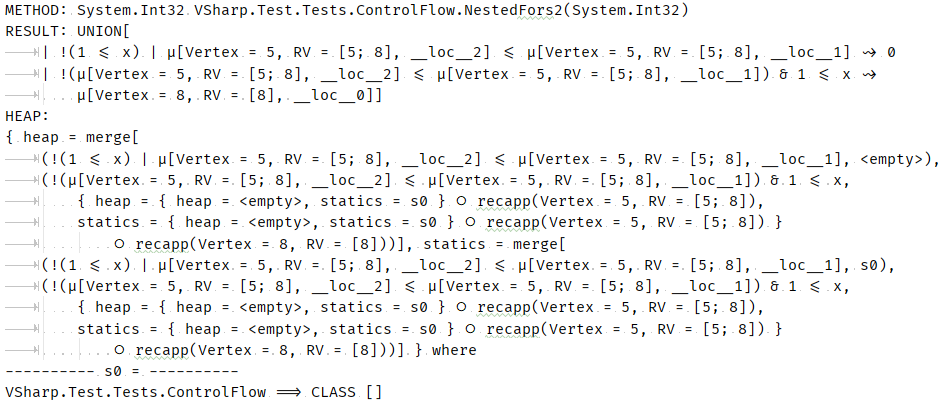
\includegraphics[scale=0.5]{Batoev/images/results.PNG}
\caption{Результат символьного исполнения метода~\ref{example:fors}}
\end{figure}

\begin{table}[t]
    \centering
    \begin{tabular}{ |p{3cm}||p{2cm}|p{2cm}|p{2cm}|  }
        \hline
        \multicolumn{4}{|c|}{Количественные характеристики тестов} \\
        \hline
        Название тестового набора &Количество тестов в наборе&Количество успешно пройденных тестов&Количество инструкций CIL\\
        \hline
        Arithmetics   &80    &77    &1968\\
        Logics        &75    &75    &1458\\
        Conditional   &10    &6     &943\\
        Recursive     &5     &5     &751\\
        Lambdas       &2     &2     &404\\
        Generic       &14    &14    &194\\
        Strings       &15    &15    &219\\
        Unsafe        &16    &16    &312\\
        Typecast      &19    &19    &969\\
        Methods       &10    &10    &238\\
        Lists         &9     &9     &1420\\
        Chess.NET     &1     &1     &2723\\
        \hline
        Всего         &256   &249   &11599\\
        \hline
    \end{tabular}
    \captionof{table}{Результаты тестирования}
    \label{experiments}
\end{table}


\FloatBarrier

\subsection{Тестирование интерпретатора}
Тестирование нового интерпретатора проводилось на тестовой подсистеме проекта <<VSharp.Test>> и на библиотеке \textsc{Chess.NET}.
Подсистема содержит тестовые наборы, затрагивающие различные конструкции и возможности языка C\#:
арифметику, логические операции,
работу с массивами разных размерностей, генерирование исключений, тесты на классы и структуры, включающие взаимодействие со статическими членами и вызовы виртуальных методов,
тесты с неограниченной рекурсией, тесты с \emph{unsafe}-кодом, тесты со строками. 

Таблица~\ref{experiments} показывает результаты проведенного тестирования. 
В наборах тестах с арифметикой и условными конструкциями была часть тестов с генерацией исключений. 
Поскольку схема обработки исключений для языка CIL не была реализована, то данные тесты были некорректно исполнены.
По той же причине не было проведено тестирования на тестовым наборе <<TryCatch>>, 
основное предназначение которого --- инициирование и перехват исключений.

\section{Заключение}

В данной работе описан подход к композициональному символьному исполнению без раскрутки. Была предложена концепция композициональной памяти с символьной адресацией. Был доказан некоторый набор свойств КСП, дающий основание для подхода в стиле систем переписывания, где символьные кучи могут сами выступать как символы. Это даёт возможность автоматически порождать уравнения на состояния, решения которых в точности отражают поведения функций, работающих с динамической памятью. Было показано как свести задачу решения уравнений на состояния к задаче проверки безопасности чистых функций второго порядка.

Данная работа нацелена на теоретические основания композиционального анализа динамической памяти. Мы оставляем апробацию этого подхода на будущее. Другим направлением будущих исследований может быть расширение нашего формализма на композициональный анализ параллельных программ.

\bibliographystyle{ugost2008ls}
\begin{thebibliography}{10}

\bibitem{baldoni2018survey}
Roberto Baldoni, Emilio Coppa, Daniele~Cono D’elia, Camil Demetrescu, and
  Irene Finocchi.
\newblock A survey of symbolic execution techniques.
\newblock {\em ACM Computing Surveys (CSUR)}, 51(3):50, 2018.

\bibitem{godefroid2007compositional}
Patrice Godefroid.
\newblock Compositional dynamic test generation.
\newblock In {\em ACM Sigplan Notices}, volume~42, pages 47--54. ACM, 2007.

\bibitem{jaffar2012tracer}
Joxan Jaffar, Vijayaraghavan Murali, Jorge~A Navas, and Andrew~E Santosa.
\newblock Tracer: A symbolic execution tool for verification.
\newblock In {\em International Conference on Computer Aided Verification},
  pages 758--766. Springer, 2012.

\bibitem{king1976symbolic}
James~C King.
\newblock Symbolic execution and program testing.
\newblock {\em Communications of the ACM}, 19(7):385--394, 1976.

\bibitem{kuznetsov2012efficient}
Volodymyr Kuznetsov, Johannes Kinder, Stefan Bucur, and George Candea.
\newblock Efficient state merging in symbolic execution.
\newblock {\em Acm Sigplan Notices}, 47(6):193--204, 2012.

\bibitem{mcmillan2010lazy}
Kenneth~L McMillan.
\newblock Lazy annotation for program testing and verification.
\newblock In {\em International Conference on Computer Aided Verification},
  pages 104--118. Springer, 2010.

\bibitem{kostyukov2018csewu}
Юрий~Олегович Костюков.
\newblock {\em Кучи как чистые функции:
  композициональное символьное исполнение
  без раскрутки}, pages 288--346.
\newblock 6. 2018.

\end{thebibliography}

\title{Композициональное символьное исполнение CIL-кода}

\titlerunning{Композициональное символьное исполнение CIL-кода}

\author{Батоев Константин Аланович}

\authorrunning{К.~А.~ Батоев}

\tocauthor{Константин Батоев}
\institute{St Petersburg State University\\
	\email{konstantin.batoev@gmail.com}}

\maketitle

% \renewcommand{\ttdefault}{cmtt}

\newsavebox\CBox
\newcommand\hcancel[2][0.1pt]{%
  \ifmmode\sbox\CBox{$#2$}\else\sbox\CBox{#2}\fi%
  \makebox[0pt][l]{\usebox\CBox}%
  \textcolor{red}{\rule[0.3\ht\CBox-#1/2]{\wd\CBox}{#1}}}

\captionsetup[figure]{name=Рисунок}

% \newtheorem*{proof}{Доказательство}

\renewcommand{\defnautorefname}{опр.}
\renewcommand{\lemautorefname}{лемм.}
\renewcommand{\remkautorefname}{зам.}
\renewcommand{\propautorefname}{св.}
\renewcommand{\exmpautorefname}{пр.}
\renewcommand{\thmautorefname}{теор.}
% \renewcommand{\crlrautorefname}{Corollary}
\renewcommand{\sectionautorefname}{разд.}
\newcommand{\algorithmautorefname}{лист.}
\newcommand{\algorithmcfname}{Листинг}
\makeatletter
\renewcommand{\ALG@name}{Листинг}
\makeatother

\algrenewcommand\alglinenumber[1]{\tiny #1:}

\lstdefinelanguage{Demo}
{
 morecomment = [l]{//}, 
 sensitive = true,
 morekeywords = {type, new, null,
   bool, int, write, read,
   fail, nop, let, alloc, in,
   if, then, else, call,
   true, false, and, or, not}
}

\definecolor{commentgreen}{RGB}{0,200,100}
\lstdefinestyle{demolang}{language=Demo,
    rulecolor=\color{blue!80!black},
    basicstyle=\ttfamily\footnotesize,
    keywordstyle=\color{blue}\ttfamily,
    stringstyle=\color{red}\ttfamily,
    commentstyle=\color{commentgreen}\ttfamily,
    numbers=left,
    numbersep=5pt,
    numberstyle=\tiny\color{black},
    escapechar=@,
    tabsize=2
}

\usemintedstyle{vs}

\counterwithin{lstlisting}{section}
\counterwithin{algocf}{section}

\fontfamily{times}
% \fontsize{10pt}{30pt}
\selectfont
\setlength{\parindent}{0em}
% \setlength{\parskip}{1em}
\renewcommand{\baselinestretch}{1.0}

\SetupFloatingEnvironment{listing}{name=Листинг}
\providecommand*{\listingautorefname}{лист.}
\renewcommand*{\figureautorefname}{рис.}
\renewcommand*{\tableautorefname}{табл.}
\SetAlgorithmName{Листинг}{лист.} 

\theoremstyle{plain}
\newtheorem{thm}{Теорема}%[section]
\newtheorem{lem}{Лемма}%[section]
% \newtheorem{crlr}{Corollary}%[section]

\theoremstyle{definition}
\newtheorem{defn}{Определение}
\newtheorem{remk}{Замечание}
\newtheorem*{remk*}{Замечание}
\newtheorem{prop}{Утверждение}
\newtheorem{exmp}{Пример}
% \newtheorem*{proof}{Доказательство}

% \newcommand{\defnautorefname}{опр.}
\newcommand{\lemautorefname}{лем.}
\newcommand{\remkautorefname}{зам.}
\newcommand{\propautorefname}{утв.}
\newcommand{\exmpautorefname}{пример}
\newcommand{\thmautorefname}{теор.}
% \renewcommand{\crlrautorefname}{Corollary}
\renewcommand{\sectionautorefname}{секция}
% \renewcommand{\algorithmautorefname}{Алгоритм}
% \renewcommand{\algorithmcfname}{Алгоритм}

% \renewcommand*{\Authsep}{\authorcr}
% \renewcommand*{\Authand}{\authorcr}
% \renewcommand*{\Authands}{\authorcr}

% \makeatletter
% \makeatother

\lstdefinelanguage{Demo}
{
 morecomment = [l]{//}, 
 sensitive = true,
 morekeywords = {new, null,
   fail, goto, halt,
   true, false, and, or, not}
}

\definecolor{commentgreen}{RGB}{0,200,100}
\lstdefinestyle{demolang}{language=Demo,
    rulecolor=\color{blue!80!black},
    basicstyle=\ttfamily\footnotesize,
    keywordstyle=\color{blue}\ttfamily,
    stringstyle=\color{red}\ttfamily,
    commentstyle=\color{commentgreen}\ttfamily,
    numbers=left,
    numbersep=5pt,
    numberstyle=\tiny\color{black},
    escapechar=@,
    tabsize=2
}

%%% For graph drawing
\definecolor {processblue}{cmyk}{0.96,0,0,0}
\definecolor {processgreen}{cmyk}{1,0,1,0}
\definecolor {processred}{cmyk}{0, 0.84, 0.80, 0.19}
\definecolor {processyellow}{cmyk}{0, 0, 1, 0}


%\newcommand{\csharp}[1]{\mintinline{csharp}{#1}}

\newcommand{\pex}{\textsc{Pex}}
\newcommand{\predator}{\textsc{Predator}}
\newcommand{\dotnet}{\textsc{.NET}}
\newcommand{\clang}{\textsc{C}}
\newcommand{\vsharp}{\textsc{V\#}}

\newcommand\addrset{loc}
\newcommand\termset{term}
\newcommand\guardset{guard}

\newcommand\eqby[1]{\mathrel{\stackrel{\mbox{\normalfont\tiny #1}}{=}}}
\newcommand\eqdef{\eqby{def}}

\newcommand\aite{ite}
\newcommand\ite[3]{\aite(#1,#2,#3)}
\newcommand\Ite[3]{\aite\big(#1,#2,#3\big)}
\newcommand\pair[2]{\langle#1, #2\rangle}
\newcommand\paiR[2]{\big\langle#1, #2\big\rangle}
\newcommand\mg[2]{#1=#2}
\newcommand\nmg[2]{#1\neq#2}
\newcommand\li[1]{LI(#1)}
\let\emptyheap\varepsilon
\newcommand\agrec{Rec}
\newcommand\agmerge{Merge}
\newcommand\agcompose{\bigcirc}
\newcommand\GRec[1]{\agrec\big(#1\big)}
\newcommand\GMerge[1]{\agmerge\big(#1\big)}
\newcommand\GCompose[2]{#1\agcompose#2}
\newcommand\agho{App}
\newcommand\gapp[1]{\agho(#1)}
\newcommand\GApp[1]{\agho\big(#1\big)}
\newcommand\aunion{\texttt{UNION}}
\newcommand\union[1]{\aunion\big(#1\big)}
\newcommand\Union[1]{\aunion\Big(#1\Big)}
\newcommand\aderef{readStore}
\newcommand\readTerm{readTerm}
\newcommand\writeTerm{writeTerm}
\newcommand\afind{find}
\newcommand\find[5]{\afind(#1,#2,#3,#4,#5)}
\newcommand\finD[5]{\afind\big(#1,#2,#3,#4,#5\big)}
\newcommand\Find[5]{\afind\Big(#1,#2,#3,#4,#5\Big)}
\newcommand\deref[2]{\aderef(#1,#2)}
\newcommand\Deref[2]{\aderef\big(#1,#2\big)}
\newcommand\compose[2]{#1\circ#2}
\newcommand\lmbd[2]{\lambda #1.#2}
\newcommand\lmbdx[1]{\lambda x.#1}
\newcommand\dom[1]{dom(#1)}
\newcommand\Dom[1]{dom\big(#1\big)}

\newcommand\Li[1]{LI\big(#1\big)}
\newcommand\amutate{writeStore}
\newcommand\amutateStack{writeStack}
\newcommand\mutate[3]{\amutate(#1,#2,#3)}
\newcommand\mutateStack[4]{\amutateStack(#1,#2,#3,#4)}
\newcommand\rdbodyext[6]{\Union{\big\{\paiR{#4\mg{#1}{#5}}{#6\big(#2(#5), xs\big)} \mid #5\in\dom{#2} \big\}\\&\qquad\qquad\qquad\cup\paiR{#4\bigwedge_{\mathclap{#5\in\dom{#2}}}{\nmg{#1}{#5}}}{#6\big(#3, xs\big)}}}
\newcommand\rdbody[4]{\rdbodyext{#1}{#2}{#3}{}{l}{#4}}
\newcommand\wrtbody[6]{\Union{&\paiR{\mg{#1}{#2}}{\writeTerm\big(#3,#4,#6\big)},
    \\&\paiR{\nmg{#1}{#2}}{\writeTerm\big(#5(#1),#4,#6\big)}}}
\newcommand{\var}[1]{\mathit{#1}}


\begin{abstract}
Известно, что наибольшую сложность в области верификации программ представляет задача доказательства корректности программ с циклическими участками кода. Опираясь на подход символьного исполнения программ и на введенные формализмы обобщённых куч в работе~\cite{kostyukov2018csewu}, данная работа представляет алгоритм композиционального символьного исполнения без раскрутки отношения перехода программ с произвольным графом потока управления. На его основе был реализован символьный интерпретатор языка CIL в проекте V\#, символьной виртуальной машине для анализа .NET. Была проведена апробация алгоритма на примерах, включающих сложные потоки управления, и интерпретатора на тестовой базе проекта VSharp.Test и на библиотеке Chess.NET.
\end{abstract}
\section*{Введение}
Поиск путей в графе с ограничением в виде формальных языков~\cite{FLCpathProblem} --- это задача, в которой формальные языки используются для задания множества искомых путей. В таком подходе каждый путь соответствует слову, состоящему из меток его рёбер, а ограничением на путь является принадлежность соответствующего ему слова некоторому заданному формальному языку.

В качестве класса формальных языков по иерархии Хомского наибольший интерес представляют контекстно-свободные языки. В отличие от регулярных они обладают большей выразительностью. Поэтому в задаче поиска путей контекстно-свободные ограничения позволяют задавать более сложные отношения между вершинами. Так, например, важный класс запросов поиска вершин, лежащих на одном уровне иерархии~\cite{zhlang-2016}, задаётся только контекстно-свободными, но не регулярными ограничениями. Запросы такого вида, как и другие запросы с контекстно-свободными ограничениями имеют широкое применение в биоинформатике~\cite{bio-application} и при обработке rdf-файлов~\cite{zhlang-2016}.

Наиболее удобным и подходящим инструментом для работы с граф\-структурированными данными являются графовые базы данных. Так же как и реляционные, графовые базы данных поддерживают свой язык запросов. С его помощью графовые базы данных позволяют решать вышеупомянутую задачу поиска путей. Но ограничения на пути, которые поддерживается в наиболее распространённых базах данных, являются в лучшем случае регулярными.

Отсутствие поддержки контекстно-свободных ограничений в графовых базах данных, во-первых, сильно ограничивает выразительность языка запросов. Во-вторых, при необходимости в более сложных запросах разработчикам приходится самим писать алгоритмы, решающие задачу контекстно-свободной достижимости для их частного случая. Так, например, Хуэй Мяо и др.~\cite{datascince-lifecycle} разработали систему хранения и отслеживания версий артефактов, возникающих при научных работах. Вся информация про артефакты хранилась в графовой базе данных. При этом при разработке возникла потребность в выполнении запросов с контекстно-свободными ограничениями для выявления взаимоотношений между различными версиями различных артефактов. Это и послужило началом статьи~\cite{datascince-lifecycle}, в которой приводятся алгоритмы решения частных запросов.

В недавнем исследовании Йохем Куйперс и др.~\cite{Kuijpers:2019:ESC:3335783.3335791} произвели сравнительный анализ наиболее известных алгоритмов поиска путей с конте\-кстно-свободными ограничениями. Алгоритмы запускались на графах, находящихся в хранилище графовой базы данных Neo4j. По результатам исследования было показано, что в контексте Neo4j алгоритмы обладают большим временем работы, и поэтому дальнейшая работа по расширению языка запросов прекратилась. При этом Рустам Азимов~\cite{Azimov:2018:CPQ:3210259.3210264} предоставил матричный алгоритм и его реализацию, которая работает за разумное время на реальных данных. Но, так как алгоритм был реализован вне контекста базы данных, его результат приняли недостаточно показательным. Поэтому вопрос о реализуемости запросов с контекстно-свободными ограничениями в графовых базах данных, а соответственно и о возможности расширения языка запросов для их поддержки остаётся открытым.

\section{Постановка задачи}
Целью данной работы является полная поддержка запросов с конте\-кстно-свободными ограничениями для графовой базы данных. А именно, необходимо предоставить пользователю возможность формулировать запросы с контекстно-свободными ограничениями в терминах одного из существующих стандартных языков запросов и исполнять их в графовой базе данных за приемлемое время. Для достижения этой цели были поставлены следующие задачи.

\begin{itemize}
    \item Выполнить обзор существующих реализаций поддержки запросов с контекстно-свободными ограничениями в графовых базах данных. В результате обзора необходимо выбрать наиболее перспективный с точки зрения производительности алгоритм решения задачи контекстно-свободной достижимости и подходящую для его интеграции базу данных. При выборе базы данных необходимо учитывать как возможность интеграции выбранного алгоритма, так и возможность поддержки одного из стандартных языков запросов, позволяющего выражать контекстно-свободные ограничения.
    \item Интегрировать выбранный на предыдущем шаге алгоритм в выбранную графовую базу данных.
    \item Расширить язык запросов выбранной базы данных конструкциями, необходимыми для выражения контекстно-свободных ограничений.
    \item Произвести замеры производительности полученного решения и сравнить его с существующими решениями.
\end{itemize}


\section{Обзор}

\subsection{Терминология}
Контекстно-свободной грамматикой называется $G = (\Sigma, N, P, S)$, где $\Sigma$ --- алфавит терминальных символов, $N$ --- алфавит нетерминальных символов, $P$ --- множество правил вида $A \rightarrow \alpha$, где $A \in N$, $\alpha \in (\Sigma \cup N)^*$, а $S \in N$ --- выделенный стартовый нетерминал.

% \gsv{про S забыли}.

Языком $L$ над алфавитом $\Sigma$ называется любое подмножество $2^{\Sigma^*}$. Языком, порождаемой грамматикой G, является множество $L(G) = \{S \xRightarrow{*} \beta, \beta \in \Sigma^*\}$, где $S \xRightarrow{*} \beta$ означает, что из нетереминала $S$ путём последовательного применения правил грамматики выводится $\beta$.

Контекстно-свободная грамматика $G = (\Sigma, N, P, S)$ находится в осла\-бленной нормальной форме Хомского, если любое её правило имеет вид $A \rightarrow BC$, где $A, B, C \in N$, либо $A \rightarrow a$, где $A \in N, a \in \Sigma$. В отличие от нормальной формы Хомского в ослабленной, во-первых, допускается присутствие стартового нетерминала $S$ в правых частях правил грамматики, во-вторых, запрещаются правила вида $S \rightarrow \epsilon$, где $\epsilon$ --- пустая строка.

% \gsv{Это не нормальная форма Хомского. У НФХ есть дополнительные ограничения. Мы называем то, что здесь, ослабленной НФХ. Важно отдельно проговорить разницу с НФХ.}

В задаче поиска путей с ограничениями в виде формальных языков дан граф $(V, E)$, разметка его рёбер $l: E \rightarrow \Sigma$ и язык $L$ над алфавитом $\Sigma$. Требуется найти множество всех пар вершин, между которыми существует путь, метки на рёбрах которого образуют слово в заданном языке. То есть требуется найти следующее множество:
\[\{(v, to): \exists p=(e_1,...,e_n) \in E^*: l(e_1)...l(e_n) \in L,~src(e_1)=v,~dst(e_n)=to\}\]
Здесь $src(e)$ и $dst(e)$ для $e \in E$ означают начальную и конечную вершину ребра $e$. В данном контексте язык $L$ называется языком ограничений.
% \gsv{У Вас вершины v и to никак с путём не связаны}

Задача поиска путей с контекстно-свободными ограничениями --- это задача поиска путей в виде формальных языков, в которой язык задаётся контекстно-свободной грамматикой.

\subsection{Графовые базы данных}
Графовые СУБД\footnote{СУБД --- Система управления базами данных} (далее просто графовые базы данных) --- это разновидность СУБД, в которой данные хранятся в виде графов. В отличие от других разновидностей, в графовых базах данных отношения между объектами так же важны, как и сами объекты.

Основной моделью представления графов в таких базах данных является gpraph property model~\cite{graph-propery-model}. В ней каждая сущность может содержать набор свойств в формате ключ-значение. Основными сущностями являются узлы и отношения. Узлы соответствуют вершинам графа и помимо свойств могут иметь несколько меток. Отношения соответствуют рёбрам и имеют ровно одну метку, которая называется типом отношения. На рисунке~\ref{fig:graph_bd_1} показан небольшой пример графа в такой модели. 

\begin{figure}[h]
\centering
    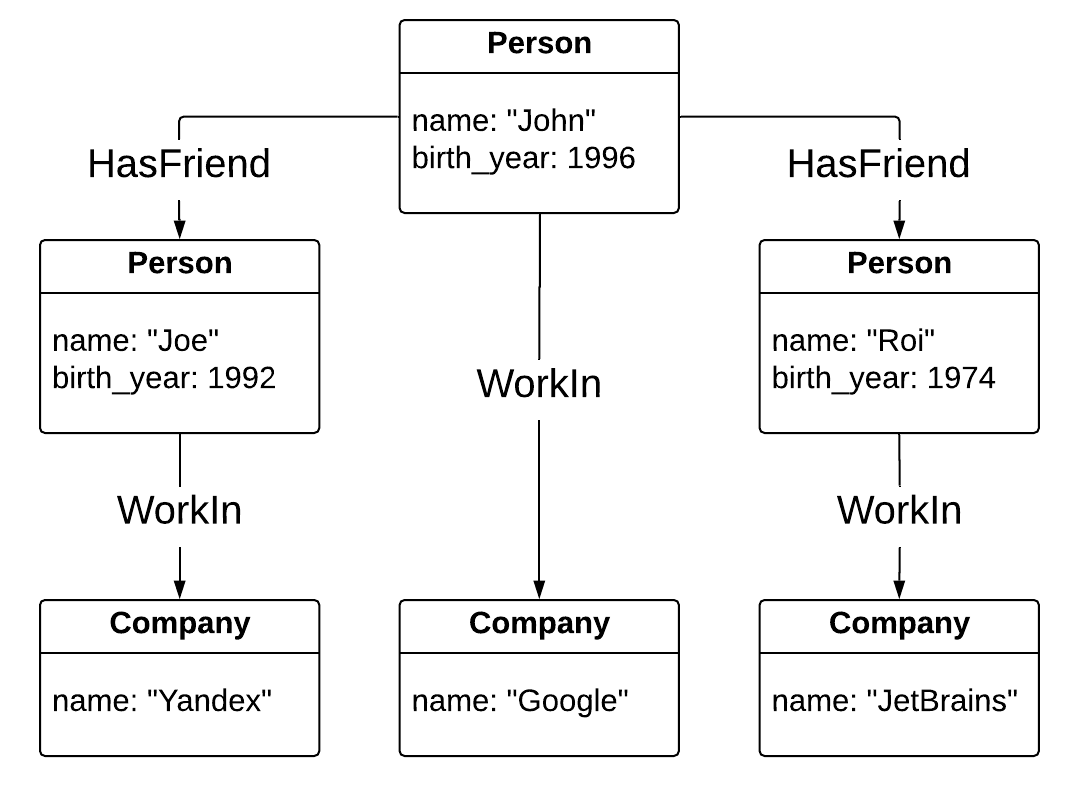
\includegraphics[width=0.7\linewidth]{Terekhov/pictures/graph_bd_1.png}
    \caption{Пример социального графа}
    \label{fig:graph_bd_1}
\end{figure}

Для работы с графами графовые базы данных предоставляют язык запросов, самым популярным из которых является Cypher~\cite{cypher-language}. В нём главный интерес представляют запросы вида сопоставления с образцом. Они позволяют задавать интересующие пути или подграфы в виде шаблонов и описывать информацию, которую нужно извлечь после удачного сопоставления. На рисунке~\ref{code:cypher_query} приведён пример такого запроса. Шаблон пути описывается в выражении MATCH. В нём между круглыми скобками задаются шаблоны вершин, а между квадратными шаблоны рёбер. Таким образом в данном примере задаются следующие ограничения: путь должен начинаться из вершины с меткой Person и именем John и состоять из двух рёбер, первое из которых должно иметь тип HasFriend, а второе WorkIn. В выражении RETURN задаётся информация, которую нужно извлечь. В данном примере это имя последней в пути вершины. В итоге ответом на такой запрос являются имена компаний, в которых работают друзья Джона. Результатом работы этого запроса на графе из рисунка~\ref{fig:graph_bd_1} является множество \{"Yandex", "JetBrains"\}.

%\lstset{
%   basicstyle=\fontsize{14}{14}\selectfont\ttfamily
%}

\begin{figure}[h]
\begin{lstlisting}[language=sql]
MATCH (p:Person)-[:HasFriend]->()-[:WorkIn]->(to)
WHERE p.name = "John"
RETURN to.name
\end{lstlisting}
\caption{Пример конечного запроса на языке Cypher}
\label{code:cypher_query}
\end{figure}

С формальной точки зрения шаблоны пути в выражении MATCH позволяют поставить задачу поиска путей с ограничениями в виде формальных языков. Так в запросе на рисунке~\ref{code:cypher_query} языком ограничений является конечный язык $\{(HasFriend, WorkIn)\}$. Для запроса на рисунке~\ref{code:cypher_query_2} ограничением является регулярный язык $\{A, B\}^*$. 

\begin{figure}[h]
\begin{lstlisting}[language=sql]
MATCH (v)-[:A | :B *]->(to)
RETURN to.name
\end{lstlisting}
\caption{Пример регулярного запроса на языке Cypher}
\label{code:cypher_query_2}
\end{figure}

При этом регулярные ограничения поддерживаются лишь частично и позволяют искать только пути произвольной длины с заданными метками на рёбрах, а более глубокие регулярные выражения не поддерживаются. Поэтому на текущий момент язык запросов довольно ограничен.

\subsection{Существующие решения}
Как было упомянуто раннее, ни одна графовая база данных не поддерживает запросов с контекстно-свободными ограничениями. Тем не менее существуют альтернативные решения поддержки таких запросов. 

\subsubsection{Парсер-комбинаторы для Neo4j}\label{sec:pareser-combinators}
В 2018 году группой исследователей из JetBrains Research на основе библиотеки Meerkat была разработана библиотека для поддержки запросов с контекстно-свободными ограничениями~\cite{parser-combinators}. Она использует графовую базу данных Neo4j~\cite{neo4j} как хранилище графов и позволяет задавать запросы в виде парсер-комбинаторов. Основным достоинством данной работы является то, что с помощью этой библиотеки кроме контекстно-свободных запросов можно выразить базовую часть языка Cypher. Но так как конкурировать с оригинальной реализацией выполнения запросов Neo4j очень сложно, это достигается вместе c сильной потерей производительности. Кроме этого контекстно-свободные запросы обрабатываются также достаточно медленно.

Таким образом данное решение является альтернативой языка запросов Neo4j, а не его расширением. Из-за медленного времени работы такое решение подходит только для работы с небольшими графами. 

\subsubsection{Расширение языка запросов SPARQL}\label{subsection:cypher-extention-2}
%Про sparql%
В 2016 Сяованг Чжан предоставил язык cfSPARQL~\cite{zhlang-2016} --- расширение языка SPARQL, который способен выразить запросы с контекстно-свободными ограничениями. Также он привёл алгоритм для вычисления таких запросов и замеры производительности. Но, во-первых, работа была сделана вне контекста графовой базы данных, а во-вторых, время работы предложенного алгоритма было больше, чем время работы парсер-комбинаторов.

\subsubsection{Существующие реализации алгоритмов решения задачи контекстно-свободной достижимости}
Основной сложностью расширения языка запросов для поддержки запросов с контекстно-свободными ограничениями является долгое время работы соответствующих алгоритмов. Так, например, в 2019 году Йохем Куйперс и другие исследователи с целью попытки расширения языка запросов Cypher для графовой базы данных Neo4j произвели сравнительный анализ производительности наиболее известных алгоритмов решения задачи контекстно-свободной достижимости.

В данном исследовании были рассмотрены и произведены замеры времени работы алгоритма Элле Хелингса~\cite{hellings-2015}, основанного на атрибутных грамматиках, восходящего алгоритма Фреда Сантоса~\cite{santos-2018}, матричного алгоритма Рустама Азимова~\cite{Azimov:2018:CPQ:3210259.3210264} и алгоритма Петтери Севона~\cite{bio-application}. Все алгоритмы были интегрированы в Neo4j и запускались на графах, находящихся в её хранилище. Алгоритмы были написаны на языке Java, при этом их реализация являлась однопоточной.

% \gsv{В таких местах надо сразу ссылку на алгоритм давать.}

По результатам замеров производительности было показано, что время работы алгоритмов является слишком большим и неприемлемым для широкого практического использования. Поэтому дальнейшая работа по интеграции и расширению языка запросов была приостановлена.

Тем не менее, матричный алгоритм Рустама Азимова в сравнительном анализе Йохема Куйперса был реализован без необходимых матричных библиотек, которые могут сильно уменьшить время его работы. Так, например, в исследовании Никиты Мишина и др.~\cite{azimov-evalution} был произведён сравнительный анализ времени работы нескольких реализаций алгоритма Рустама Азимова, основанных на различных специализированных матричных библиотеках. Графы и запросы к ним были взяты из объемлющего набора данных CFPQ\_Data~\cite{cfpq-data}, предоставленного лабораторией языковых инструментов JetBrains Research. 

Результаты замеров Никиты Мишина и др. показали, что при грамотной реализации алгоритма Рустама Азимова и использовании подходящих матричных библиотек можно добиться очень высокой производительности. Поэтому, так как основной проблемой применимости запросов с контекстно-свободными ограничениями является долгое время работы соответствующих алгоритмов, в качестве алгоритма решения задачи конте\-кстно-свободной достижимости был выбран матричный алгоритм Рустама Азимова.

\subsection{Матричный алгоритм Рустама Азимова}\label{sec:matrix-algo}
Выбранный в предыдущей главе алгоритм Рустама Азимова~\cite{Azimov:2018:CPQ:3210259.3210264}, в отличие от других алгоритмов решения задачи контекстно-свободной достижимости~\cite{hellings-2015, santos-2018, zhlang-2016}, работает с графами в виде разреженных матриц смежности. Данный алгоритм состоит из последовательности операций над разреженными матрицами, время работы которых зависит не от размеров матричных операндов, а от количества их ненулевых элементов.

На вход алгоритму (см. алгоритм 1) поступает помеченный граф $D=(V,E)$ и контекстно-свободная грамматика $G=(\Sigma, N, P, S)$ в ослабленной нормальной форме Хомского. Для каждого нетерминала $A$ в ассоциативном массиве $T$ хранится соответствующая ему булева матрица $T[A]$. На всём этапе алгоритма поддерживается следующий инвариант: $T[A]_{i,j} = 1$ равносильно существует пути, метки на рёбрах которого образуют слово, выводящееся из нетерминала $A$. На первом этапе происходит инициализация матриц с помощью простых правил грамматики, после чего инвариант выполняется для всех путей единичной длины. На втором этапе происходит транзитивное замыкание, после чего этот инвариант верен для всех путей. Результатом данного алгоритма является матрица, соответствующая стартовому нетерминалу $S$.

%  Это позволяет для его реализации использовать многопоточные матричные библиотеки, с помощью которых можно добиться очень высокой производительности. Поэтому на текущий момент алгоритм Рустама Азимова показывает наилучшее время работы на практике.

\begin{algorithm}
\caption{Матричный алгоритм Рустама Азимова}

\begin{algorithmic}[1]
\Function{contextFreePathQuerying}{$D$, $G$}
    \State{$n =$ getNodeCount(D)}
    \State{$N =$ getAllNonterms(G)}
    \State{$E =$ getEdges($D$)}
    \State{$P =$ getRules($G$)}
    \State{$S =$ getStartNonterm($G$)}
    \State{$T = \{A \rightarrow \varnothing_{n \times n} : A \in$ $N$ \} }
    \ForAll{$(v, to, label) \in E$}
    \Comment{Инициализация матриц}
        \ForAll{$A \rightarrow label \in P$}
            \State{$T[A]_{i,j} = 1$}
        \EndFor
    \EndFor    
    \While{$\exists A: T[A]$ is changing}
    \Comment{Вычисление замыкания}
        \ForAll{$A \rightarrow BC \in P$}
            \State{$T[A] \oplus= T[B] \otimes T[C]$}
        \EndFor
    \EndWhile
\State \Return $T[S]$
\EndFunction

\end{algorithmic}
\end{algorithm}

Практическое время работы алгоритма Рустама Азимова сильно зависит от производительности используемой матричной библиотеки. Это накладывает некоторые ограничения на выбор подходящей графовой базы данных, так же как и возможность представления графов в матричном виде.

\subsection{RedisGraph}
RedisGraph~\cite{redis-graph} --- это высокопроизводительная графовая база данных, поддерживающая язык запросов Cypher. В отличие от наиболее распространённой графовой базы данных Neo4j~\cite{neo4j}, RedisGraph написан на языке Си и для работы с данными использует Redis~\cite{redis}, основным достоинством которого является возможность хранить данные прямо в оперативной памяти. Это позволяет RedisGraph быстро обрабатывать пользовательские запросы.

Также RedisGraph является единственной графовой базой данных, которая работает с графами в виде разреженных матриц смежности и транслирует запросы языка Cypher в матричные выражения. Для представления графов в таком виде и работы с ними в терминах линейной алгебры используется мощный матричный фреймворк GraphBlas~\cite{graph-blas}. Его реализация SuiteSparse~\cite{suite-sparse} является многопоточной и сильно оптимизирована, что позволяет RedisGraph добиться высокой производительности.

Из всего этого следует, что RedisGraph идеально подходит для интеграции матричного алгоритма. Во-первых, графы представляются в необходимом алгоритму виде, что позволит избежать издержек на конвертацию форматов. Во-вторых, использование SuiteSparse для вычисления матричных операций позволит добиться высокой производительности. Поэтому RedisGraph был выбран в качестве графовой базы данных для интеграции матричного алгоритма и расширения языка запросов.

% Так как алгоритм Рустама Азимова работает с матричным представлением графа,, как наиболее подходящий для интеграции матричного алгоритма.

\subsection{Расширение языка Cypher}\label{subsection:cypher-extention}
На текущий момент оригинальная версия языка Cypher, используемая в том числе и в RedisGraph, не поддерживает запросов с контекстно-свободными ограничениями. Но тем не менее в 2017 году был разработан черновой вариант спецификации расширения Cypher~\cite{cypher-specification}, которая вводит в язык шаблоны путей. Они позволяют выразить более сложные запросы, в том числе запросы с контекстно-свободными ограничениями.

Шаблоны путей являются альтернативой шаблонам рёбер, которые есть в оригинальном Cypher. Они, как и шаблоны рёбер, могут встречаться в выражении MATCH и иметь своё направление. Кроме этого в глобальной области запроса им можно задавать имя, на которое потом можно ссылаться внутри других шаблонов.

Шаблон пути представляет из себя регулярное выражение над некоторыми примитивами. В качестве таких примитивов могут выступать шаблоны рёбер, шаблоны вершин и ссылки на именованные шаблоны путей. Также любым подвыражениям можно задавать своё направление. Основная часть конкретного синтаксиса данного расширения приведена на рисунке~\ref{fig:cypher_syntax}.

\begin{figure}[]
\begin{align*}
\begin{split}
PathPattern     &= ["<"],~"-/",~PathExpression,~"/-",~[">"]\\
PathExpression  &= \{PathAlternative\}\\
PathAlternative &= PathRepetition,~\{"|", PathRepetition\}\\
PathRepetition  &= ["<"],~PathBase,~[">"],~("*")
\end{split}\\
\begin{split}
PathBase &= PathEdge \\
         &~~|~PathNode \\
         &~~|~PathReference \\
         &~~|~"[",~PathExpression,~"]"
\end{split}\\
\begin{split}
PathEdge      &= Label \\
PathNode      &= "(",~[Label,~\{"|",~Label\}],~")" \\
PathReference &= "\sim",~SymbolicName; \\
Label         &= ":",~LabelName
\end{split}
\end{align*}
\caption{Расширение конкретного синтаксиса Cypher}
\label{fig:cypher_syntax}
\end{figure}

Каждый шаблон пути задаёт отношение на множестве вершин. Поэтому семантикой языка шаблонов путей $L_{P}$ в контексте графа $G(V, E)$ является отображение $\llbracket \cdot \rrbracket_{G}: L_P \rightarrow V \times V$, которое каждому шаблону $p\in L_P$ сопоставляет множество пар вершин, между которыми существует путь, удовлетворяющий данному шаблону $p$. 

Подробное описание данной семантики приводится в таблице~\ref{tab:cypher_sematic}.  В ней наибольший интерес представляют именованные шаблоны путей, так как именно с помощью них можно выразить запросы с контекстно-свободными ограничениями. Все именованные шаблоны путей $S_i = p_j$ можно рассматривать как правила контекстно свободной грамматики с алфавитом нетерминалов $\{S_i\}_{i=1}^n$. Тогда каждый нетерминал $S_j$ порождает язык $L_{S_j} \subset L_p$, а семантикой соответствующего именованного шаблона пути $S_j=p_j$ является множество $\bigcup\limits_{p \in L_{s_j}} \llbracket p \rrbracket_{G}$.

На рисунке~\ref{code:cypher_query_3} приведён пример запроса в расширенном синтаксисе. В нём декларируется именованный шаблон S, который задаёт множество правильных скобочных последовательностей над ребрами с типом L и R. Далее в выражении MATCH задаётся шаблон пути, состоящий из ссылки на шаблон S. Таким образом результатом обработки запроса является множество всех пар вершин, между которыми существует путь, метки на рёбрах которого образуют правильную скобочную последовательность. 

\begin{table}[h!]
\begin{adjustbox}{max width=\textwidth}
\begin{tabular}{|c|c|c|}
\hline
$p \in L_P$                                                                                  & $\llbracket p \rrbracket_{G}$                                                                                                                                                                                   & Описание шаблона пути                                                                                                         \\ \hline
\hline
()                                                                                            & $\{(v, v): v \in V\}$                                                                                                                                                                                           & \begin{tabular}[c]{@{}c@{}}Пустой путь, состоящий из \\ одной произвольной вершины\end{tabular}                               \\ \hline
:a                                                                                            & $\{e=(v,to): e \in E, type(e)=a\}$                                                                                                                                                                              & \begin{tabular}[c]{@{}c@{}}Путь единичной длины,\\  состоящий из ребра с типом $a$\end{tabular}                               \\ \hline
(:b)                                                                                          & $\{(v, v): v \in V, label(v)=b\}$                                                                                                                                                                               & \begin{tabular}[c]{@{}c@{}}Пустой путь, состоящий из одной\\  вершины, помеченной меткой $b$\end{tabular}                     \\ \hline
$\alpha~\beta$                                                                                & $\llbracket \alpha \rrbracket_{G}\circ \llbracket \beta \rrbracket_{G}$                                                                                                                                         & Конкатенация путей $\alpha$ и $\beta$                                                                                         \\ \hline
$\alpha~|~\beta$                                                                              & $\llbracket \alpha \rrbracket_{G}\cup \llbracket \beta \rrbracket_{G}$                                                                                                                                          & Альтренатива между путями $\alpha$ и $\beta$                                                                                  \\ \hline
$[\alpha]$                                                                                    & $\llbracket \alpha \rrbracket_{G}$                                                                                                                                                                              & \begin{tabular}[c]{@{}c@{}}Квадратные скобки позволяют \\ группировать  выражения \\ для задания ассоциативности\end{tabular} \\ \hline
\textless{}$\alpha$                                                                           & $\{(to, v): (v, to) \in \llbracket \alpha \rrbracket_{G}\}$                                                                                                                                                     & Путь, обратный к пути $\alpha$                                                                                                \\ \hline
\textless{}$\alpha$\textgreater{}                                                             & $\llbracket \alpha~|~$\textless{}$\alpha \rrbracket_{G} $                                                                                                                                                       & \begin{tabular}[c]{@{}c@{}}Альтернатива между путём $\alpha$ и\\ обратным к нему\end{tabular}                                 \\ \hline
$\alpha^*$                                                                                    & $\llbracket \alpha \rrbracket_{G}^{*}$                                                                                                                                                                          & \begin{tabular}[c]{@{}c@{}}Путь, состоящий из\\ конкатенации 0 или более путей $\alpha$\end{tabular}                          \\ \hline
\begin{tabular}[c]{@{}c@{}}$\{S_i = p_i\}_{i=1}^{n}$\\ -- named\\  path patterns\end{tabular} & \begin{tabular}[c]{@{}c@{}}$P = \{S_i \rightarrow p_i\}_{i=1}^n$\\ $Gram_j = (\Sigma, \{S_i\}_{i=1}^n, P, S_j)$\\ $\llbracket S_j \rrbracket_{G} = \bigcup\limits_{p \in L(G)}{\llbracket p \rrbracket_{G}}$\end{tabular} & Именнованые шалоны путей                                                                                                      \\ \hline
$\sim$$S$                                                                                     & $\llbracket S \rrbracket_{G}$                                                                                                                                                                                   & \begin{tabular}[c]{@{}c@{}}Ссылка на именнованный\\  шаблон пути\end{tabular}                                                 \\ \hline
\end{tabular}
\end{adjustbox}
\caption{Семантика языка шаблонов путей}
\label{tab:cypher_sematic}
\end{table}

\begin{figure}[h!]
\begin{lstlisting}[language=sql]
PATH PATTERN S = ()-/ [:L ~S :R] | [~S ~S] | () /-()
MATCH (v)-/ ~S /-(to)
RETURN v, to
\end{lstlisting}
\caption{Пример запроса в расширенном синтаксисе Cypher}
\label{code:cypher_query_3}
\end{figure}

Данная спецификация расширения Cypher была представлена официальными разработчиками и сильно расширяет выразительность языка, предоставляя удобную возможность выражать запросы как с регулярными, так и с контекстно-свободными ограничениями. Поэтому в моей работе приводится поддержка выполнения запросов именно для этого расширения языка.

% \gsv{Не хватает какого-то чёткого вывода про то, что вот именно это мы и буем использовать.}

\section{Реализация}
По результатам обзора было решено реализовать поддержку расширения языка Cypher, представленную в главе~\ref{subsection:cypher-extention}, для графовой базы данных RedisGraph. За основу алгоритма, решающего задачу поиска путей с контекстно-свободными ограничениями, был взят матричный алгоритм Рустама Азимова, описанный в главе~\ref{sec:matrix-algo}.

% \gsv{И зжесь надо ещё раз подитожить в духе "по результатм обзора было решено сделать то и это с использованием того и сего"}

\subsection{План выполнения запроса}\label{execution-plan}
В RedisGraph основной частью обработки запроса является построение плана его выполнения. Её часть, которая относится к шаблонам путей приведена на рисунке~\ref{fig:execution_plan}. В ней зелёным цветом выделено то, что было добавлено или расширено.

В самом начале, после получения запроса строится его абстрактное синтаксическое дерево \textit{AST}. Далее, из него извлекаются именованные и неименованные шаблоны путей \textit{PathPattern} и \textit{NamedPathPatterns}, после чего они преобразуются в более удобное промежуточное представление \textit{PathExpr}. При этом, для дальнейшего связывания ссылок, именованные шаблоны сохраняются в глобальном контексте запроса \textit{PathPatternCtx}.

На следующем этапе происходит трансляция промежуточных представлений \textit{PathExpr} в матричные выражения \textit{AlgebraicExpression}. В них операндами являются либо матрицы, полученные из указанного в запросе графа \textit{GraphCtx}, либо ссылки на именованные шаблоны путей из \textit{PathPatternCtx}. Основной идеей трансляции является то, что после вычисления матричного выражения получается матрица, которая задаёт то же самое отношение на множестве вершин, что и исходный шаблон пути.

Далее каждое такое выражение формирует новую операцию плана выполнения запроса \textit{CfpqTraverseOp}. При её вычислении сначала происходит запуск расширенной версии матричного алгоритма Рустама Азимова. Он решает задачу контекстно-свободной достижимости, заданной именованными шаблонами путей. После этого все ссылки в матричном выражении заменяются на полученные в ходе алгоритма матрицы и происходит вычисление матричного выражения. Каждая такая операция добавляется в план выполнения запроса.

%  \gsv{Используйте \textit{CfpqTraverseOp} вместо долларов для длинных слов. Они тогда не распадаются из-а лишних пробелов.}

\begin{figure}[H]
\centering
    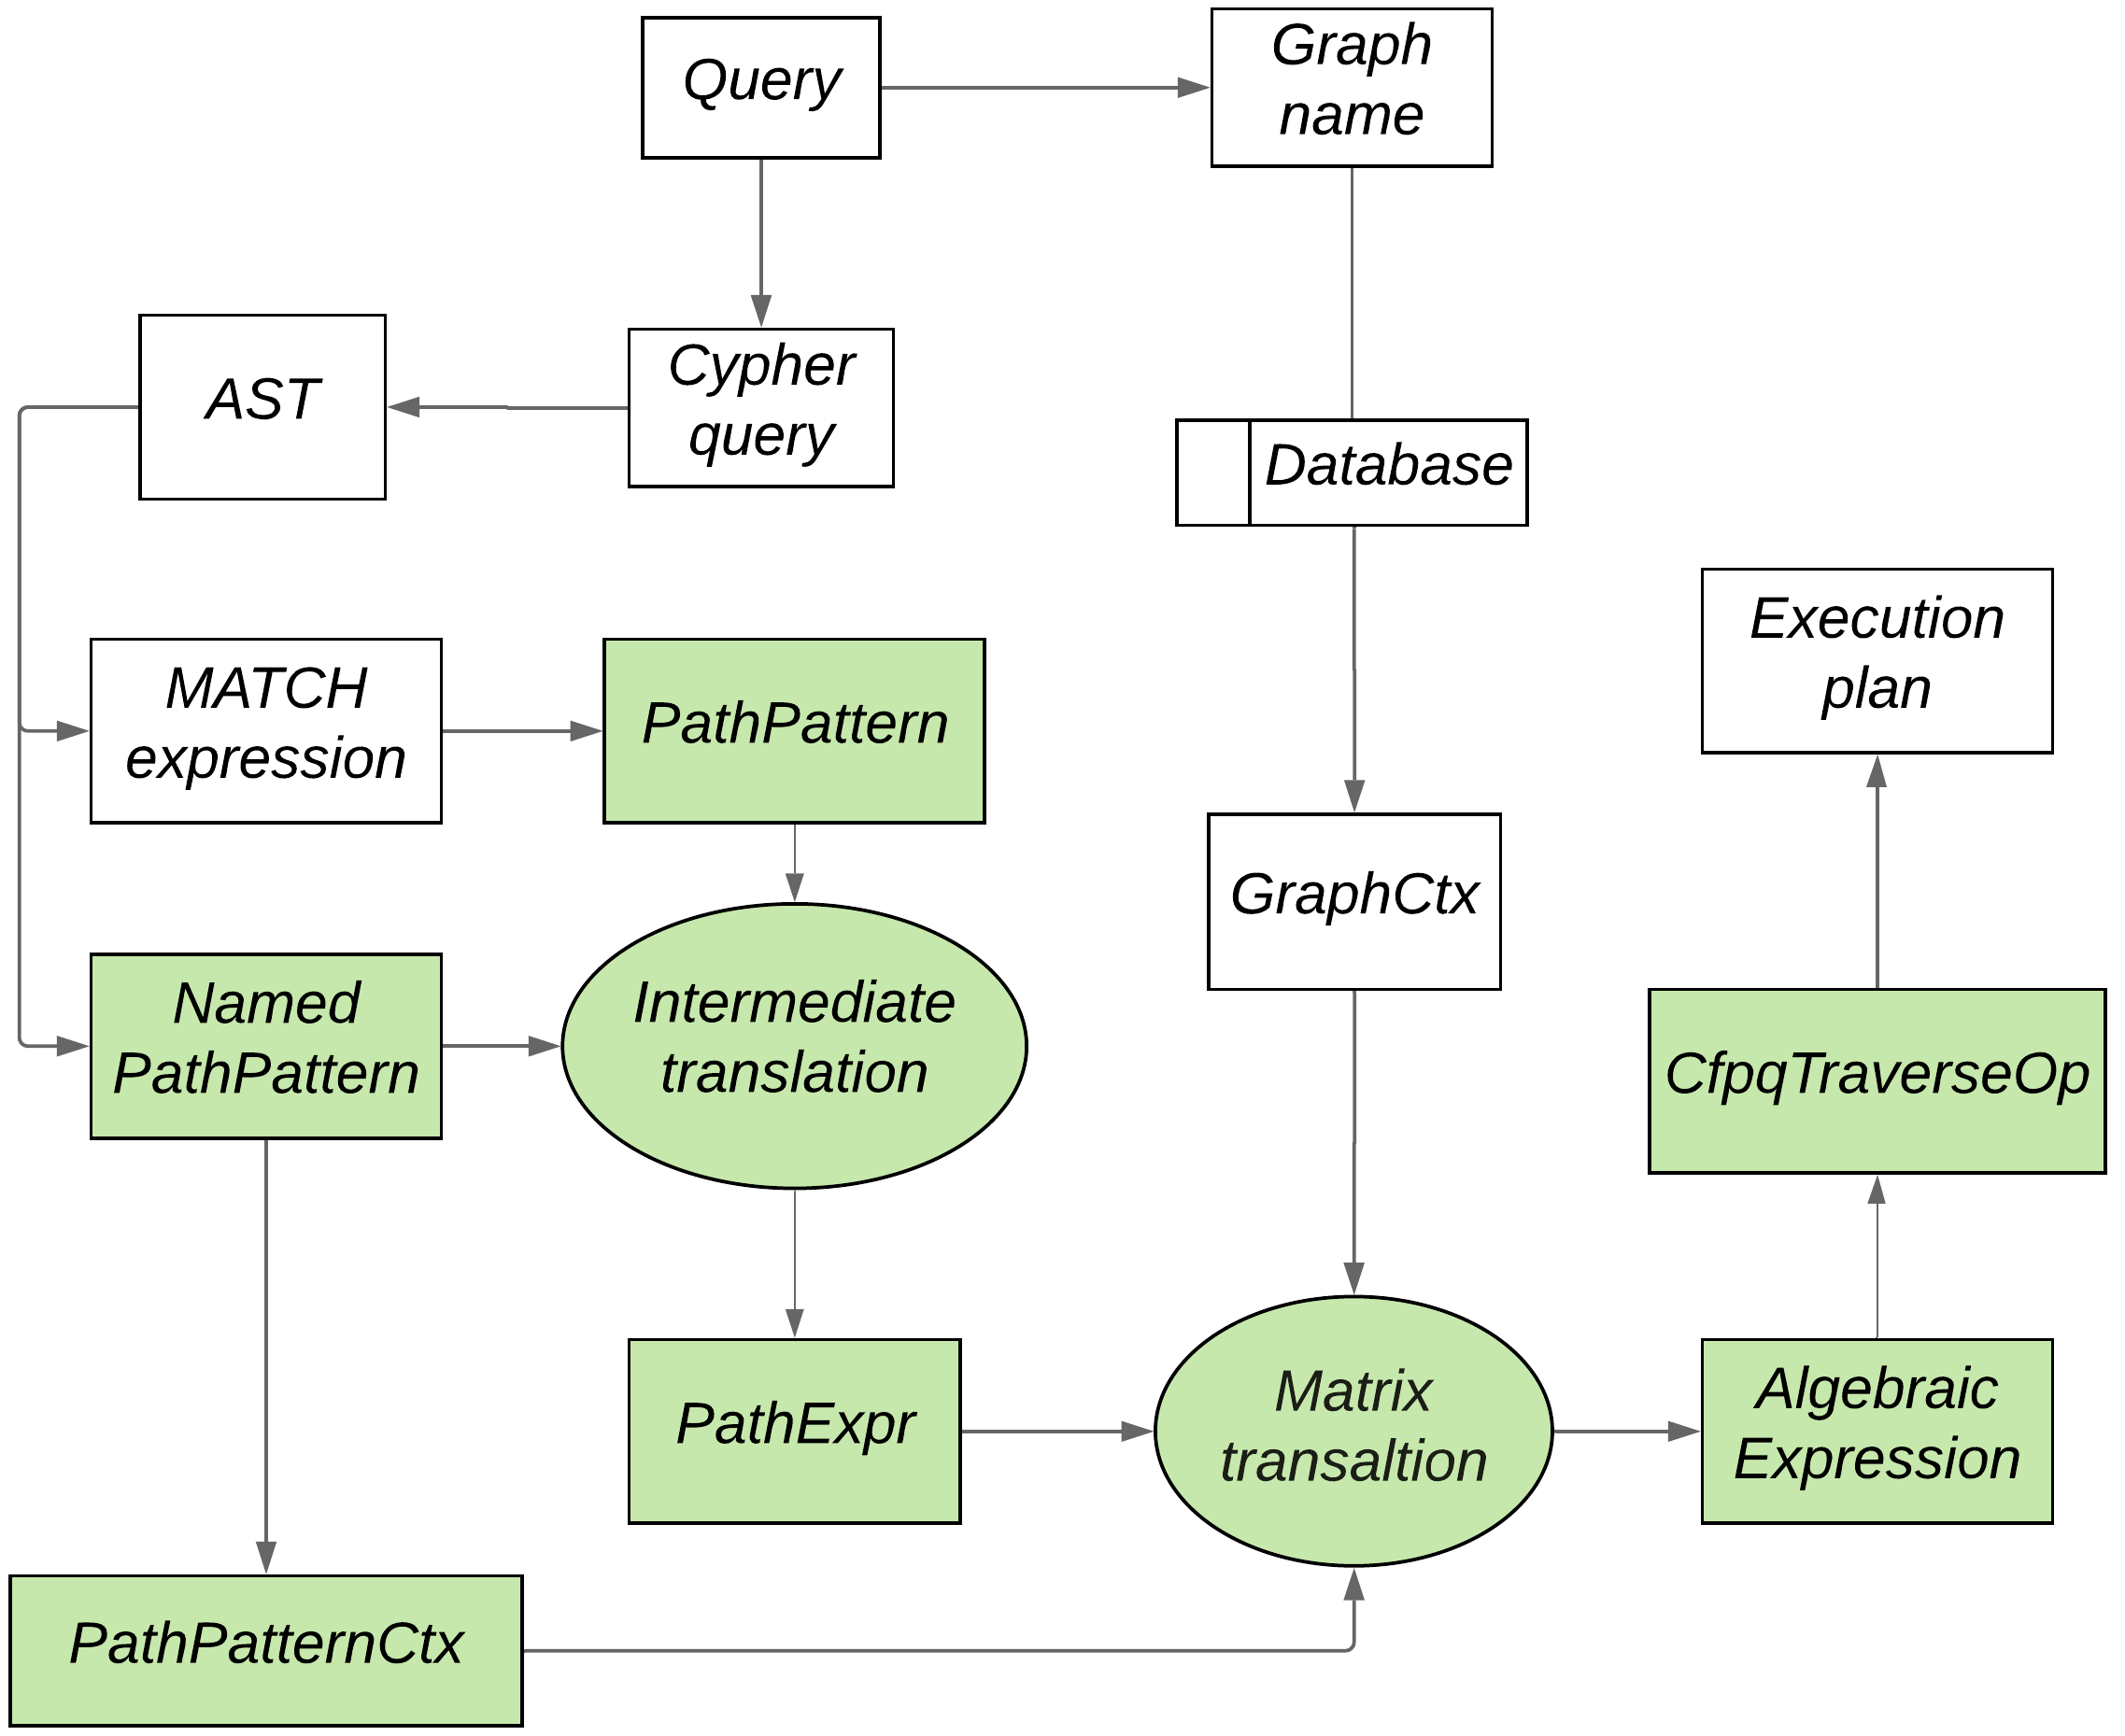
\includegraphics[width=1.0\linewidth]{Terekhov/pictures/execution_plan_3.png}
    \caption{Расширение построения плана выполнения запроса}
    \label{fig:execution_plan}
\end{figure}

\subsection{Промежуточное представление}\label{matrix-translation}
Шаблоны путей, полученные из \textit{AST}, транслируются в промежуточное представление \textit{PathExpr}. Оно позволяет задавать более простой абстрактный синтаксис, который описан на рисунке~\ref{fig:intermidiate_repr}. 

Таким образом, альтернативе и конкатенации шаблонов соответствуют \textit{PathAlt} и \textit{PathSeq}, \textit{PathGroup} позволяет задавать направление пути и наличие замыкания, а \textit{PathBasic} соответствует либо примитивным шаблонам \textit{PathNode}, \textit{PathEdge} и \textit{PathRef}, либо целому выражению \textit{PathExpr}. Примеры промежуточного представления шаблонов приведены в таблице~\ref{tab:inter_examples}.
\begin{figure}[h!]
\begin{align*}
\begin{split}
PathExpr=~ &PathSeq(PathExpr,~PathExpr)~|\\
           &PathAlt(PathExpr,~PathExpr)~|\\
           &PathGroup(PathBasic, direction, range)
\end{split}\\
\begin{split}
PathBasic=~ &PathNode(label)~|\\
            &PathEdge(type)~~|\\
            &PathRef(name) ~~|\\
            &PathExpr
\end{split}\\
\begin{split}
direction \in ~&\{inbound,~outbound,~bidirectional\}\\
range \in     ~&\{*, \varnothing\}
\end{split}
\end{align*}
\caption{Промежуточное представление PathExpr}
\label{fig:intermidiate_repr}
\end{figure}

\begin{table}[h]
\centering
\begin{adjustbox}{max width=\textwidth}
\begin{tabular}{|c|l|}
\hline
$L_p$                        & \multicolumn{1}{c|}{PathExpr}                                                                                                        \\ \hline
{[}:A :B{]} | (:C)           & \begin{tabular}[c]{@{}l@{}}$PathAlt($\\ $~~~~PathSeq(PathEdge("A"),~PathEdge("B"))$\\ $~~~~PathNode("C")$\\ $)$\end{tabular}         \\ \hline
\textless{}{[}:A $\sim$S{]}* & \begin{tabular}[c]{@{}l@{}}$PathGroup($\\ $~~~~PathSeq(PathEdge("A"),~PathRef("S")),$\\ $~~~~inbound,$\\ $~~~~*,$\\ $)$\end{tabular} \\ \hline
\end{tabular}
\end{adjustbox}
\caption{Примеры промежуточного представления запросов}
\label{tab:inter_examples}
\end{table}

\newpage
\subsection{Трансляция в матричные выражения}
Как было упомянуто ранее, RedisGraph представляет графы в виде разреженных матриц. А именно каждый граф $G$ задаётся следующей тройкой $(A \in M_{n\times n},~lab \in Labels \rightarrow Diag_n,~rel \in RelTypes \rightarrow M_{n \times n})_G$. Здесь $M_{n \times n}$ означает полукольцо булевых матриц, а $Diag_n$ полукольцо диагональных булевых матриц. Матрица $A$ служит матрицей смежности графа, а отображения $lab$ и $rel$ сопоставляют меткам вершин и типам рёбер соответствующие булевы матрицы. Таким образом, ребро $(v, to)$ графа $G$ имеет тип $a$ тогда и только тогда, когда $rel(a)_{v,to} = 1$.  Таким же образом, принадлежность метки $l$ вершине $v$ равносильно $lab(l)_{v,v}=1$.

Любую булеву матрицу $M$, участвующую в задании графа $G(V, E)$, можно рассматривать как отношение на множестве вершин $R(M) = \{(v, to):~M_{v,to}=1\}$. Операциями сложения и умножения в булевом полукольце являются дизъюнкция и конъюнкция. Поэтому умножению матриц $A*B$ соответствует композиция отношений $R(A) \circ R(B)$, сложению $A+B$ соответствует объединение отношений $R(A) \cup R(B)$, а транспонированная матрица $A^T$ соответствует обратному к R(A) отношению $R(A)^{-1}$. Такая взаимосвязь между матричными операциями и отношениями лежит в основе алгоритма трансляции, приведённом на рисунке~\ref{algo:translation}.

Данный алгоритм является рекурсивным и принимает на вход промежуточное представление шаблона пути $expr$, представление графа $g$ и контекст именованных шаблонов путей $pathCtx$. Целевым языком трансляции является простой язык матричных выражений, приведённый на рисунке~\ref{fig:alg-expr}.

Базовым случаем рекурсии являются примитивные шаблоны \textit{Path\-Node}, \textit{PathEdge} и \textit{PathReference}, которые транслируются в операнды матричного выражения. Для первых двух соответствующие матрицы извлекаются из графа с помощью функций \textit{GetLabel\-Matrix} и \textit{GetRelation\-Matrix}. При этом случай $label = \varnothing$ соответствует шаблону пути, состоящему из одной произвольной вершины. Поэтому такой путь задаётся тождественным отношением $R(I)$, где $I$ --- единичная матрица. Для \textit{Path\-Reference} создаётся ссылка на матрицу именованного шаблона, которая будет вычислена на следующем этапе при выполнении алгоритма контекстно-свободной достижимости.

Трансляция для шаблонов \textit{PathSeq} и \textit{PathAlt} происходит одинаковым образом --- сначала происходит трансляция дочерних шаблонов, а потом из полученного результата образуются операции умножения или сложения. Такая трансляция обосновывается семантикой шаблонов альтернативы и конкатенации, приведенной в главе~\ref{subsection:cypher-extention}, и связью отношений с матричными операциями, описанными раннее.

Наиболее интересным случаем является трансляция \textit{Path\-Group}, так как в некоторых случаях контекст именованных шаблонов $pathCtx$ расширяется. В начале происходит трансляция дочернего шаблона. Далее, если заданное направление является обратным, к полученной матрице применяется операция транспонирования. Если же направление является произвольным, то формируется операция сложения из полученной матрицы и транспонированной к ней. Это соответствует альтернативе между прямым путём и обратным к нему. После этого при отсутствии замыкания результат возвращается. Иначе происходит трансляция замыкания полученного выражения. Так как его нельзя выразить через имеющиеся матричные операции, создаётся новый именованный шаблон, а замыкание заменяется ссылкой на него. Нетрудно показать, что регулярное выражение $R^*$ и контекстно-свободная грамматика с одним правилом $S \rightarrow R~S \mid \epsilon$ равносильны. Поэтому правая часть этого правила тривиальным образом сразу же транслируется в выражение \textit{Add(Mul(R, MatrixRef(S)), I)} и добавляется в \textit{pathCtx} вместе с полученным новым именем.

Таким образом, после работы данного алгоритма из промежуточного представления шаблона пути получается выражение над матрицами. При дальнейшем его вычислении получается матрица, которая соответствует такому же отношению на множестве вершин, как и семантика изначального шаблона.

\algnewcommand\algorithmicswitch{\textbf{switch}}
\algnewcommand\algorithmiccase{\textbf{case}}
\algnewcommand\algorithmicof{\textbf{of}}
\algnewcommand\algorithmicassert{\texttt{assert}}
\algnewcommand\algorithmiccasepart{\texttt{:}}
\algnewcommand\Assert[1]{\State \algorithmicassert(#1)}%
% New "environments"
\algdef{SE}[SWITCH]{Switch}{EndSwitch}[1]{\algorithmicswitch\ #1}{\algorithmicend\ \algorithmicswitch}%
\algdef{SE}[CASE]{Case}{EndCase}[1]{\algorithmiccase\ #1\algorithmiccasepart}{\algorithmicend\ \algorithmiccase}%
\algdef{SE}[CASEPART]{CasePart}{EndCasePart}[1]{#1\algorithmiccasepart}{\algorithmicend\ \algorithmiccasepart}%
\algtext*{EndSwitch}%
\algtext*{EndCase}%
\algtext*{EndCasePart}%

\begin{algorithm}
\caption{Алгоритм трансляции}
\begin{algorithmic}[1]
\Function{translate}{PathExpr expr, GraphCtx g, PathPatternCtx pathCtx}
    \Switch{expr}
        \Case{$PathNode$(label)}
            \If{label $== \varnothing$}
                \State \Return \Call{GetIdentityMatrix}{g}
            \Else
                \State \Return \Call{GetLabelMatrix}{g, label}
            \EndIf
        \EndCase
        \Case{$PathEdge$(type)}
            \State \Return \Call{GetRelationMatrix}{g, type}
        \EndCase
        \Case{$PathRef(name)$}
            \State \Return $MatrixRef$(name)
        \EndCase
        \Case{$PathSeq$(left, right)}
            \State \Return Add(\Call{translate}{left}, \Call{translate}{right})
        \EndCase
        \Case{$PathAlt$(left, right)}
            \State \Return Mul(\Call{translate}{left}, \Call{translate}{right})
        \EndCase
        \Case{$PathGroup$(basic, dir, range)}
            \State res = \Call{translte}{basic}
            \Switch{dir}
                \Case{$inbound$}
                    \State res = $Transpose$(res)
                \EndCase
                \Case{$bidirectional$}
                    \State res = $Add$(res, $Transpose$(res))
                \EndCase
            \EndSwitch
            \Switch{range}
                \Case{ $\varnothing$}
                    \State \Return res
                \EndCase
                \Case{$*$}
                    \State name = \Call{AllocateNewPathPattern}{ctx}
                    \State res = $Mul$(res, $MatrixRef$(name))
                    \State res = $Add$(res, \Call{GetIdentityMatrix}{g})
                    \State \Call{SetPathPetternExpression}{p, name, res}
                    \State \Return $MatrixRef$(name)
                \EndCase
            \EndSwitch
        \EndCase
    \EndSwitch
\EndFunction
\end{algorithmic}
\caption{Алгоритм транслции в матричные выражения}
\label{algo:translation}
\end{algorithm}

\begin{figure}[H]
\begin{align*}
\begin{split}
AlgExpr= ~ &Add(AlgExpr, AlgExpr)~|\\
           &Mul(AlgExpr, AlgExpr)~|\\
           &Transpose(AlgExpr)~|\\
           &Matrix~|\\
           &MatrixRef(ref)
\end{split}
\end{align*}
\caption{Алгебраическое выражение над матрицами}
\label{fig:alg-expr}
\end{figure}

\subsection{Формирование и вычисление операции плана выполнения}
После этапа трансляции в RedisGraph происходит построение плана выполнения запроса. Он формируется из последовательности операций, которые выполняют базовые вычисления. Для поддержки шаблонов путей была добавлена операция \textit{CfpqTraverseOp}. Она создаётся для каждого матричного выражения, полученного на предыдущем шаге из неименованого шаблона пути, и отвечает за его вычисление.

На этапе инициализации новой операции \textit{CfpqTraverseOp} из соответствующего матричного выражения рекурсивно извлекаются все ссылки на именованные шаблоны путей, от которых зависит данное выражение. После этого они поступают на вход алгоритма, решающего задачу контекстно-свободной достижимости (см. алгоритм 4).

Этот алгоритм является расширенной версией матричного алгоритма Рустама Азимова, приведенного в главе~\ref{sec:matrix-algo}. В данном алгоритме, в отличие от алгоритма Рустама Азимова, не требуется задавать правила грамматики в ослабленной нормальной форме Хомского. Вместо этого правая часть правила задаётся с помощью промежуточного представления \textit{PathExpr}. При этом подразумевается, что для любого именованного шаблона $p$ из глобального контекста \textit{pathCtx} его промежуточное представление уже транслировано в матричное выражение и записано в \textit{pathCtx[p].algExpr}.

Принцип работы алгоритма остаётся прежним. На каждой итерации для всех невычисленных шаблонов происходит вычисление матричного выражения. Если результирующая матрица не изменяется, то она является окончательной для данного именованного шаблона и он больше не участвует в обновлении. Иначе соответствующая матрица перезаписывается.

После работы данного алгоритма все ссылки на именованные шаблоны путей в матричном выражении заменяются на подсчитанные алгоритмом матрицы, после чего происходит вычисление матричного выражения. Результат сохраняется в операции $CfpqTraverseOp$ и участвует в вычислении плана выполнения запроса наряду с результатами других операций. 
\begin{algorithm}
\begin{algorithmic}[1]
\Function{CfpqTraverseNew}{String[] patterns, PathPatternCtx pathCtx}
\While{$\exists$ p $\in$ patterns: !pathCtx[p].isEvaluated}
    \ForAll{p $\in$ patterns}
        \If{!pathCtx[p].isEvaluated}
            \State new\_matrix = \Call{EvalueteAlgExpr}{pathCtx[p].expr}
            \If{new\_matrix == pathCtx[p].matrix}
                \State pathCtx[p].isEvaluated = true
            \Else
                \State pathCtx[p].matrix = new\_matrix
            \EndIf
        \EndIf
    \EndFor
\EndWhile
\EndFunction
\end{algorithmic}
\label{algo:matrix-extention}
\caption{Расширенный матричный алгоритм}
\end{algorithm}


\section{Замеры производительности}
После реализации поддержки нового синтаксиса шаблонов путей были произведены замеры производительности.

\subsection{Сравнение с парсер-комбинаторами}\label{sec:parse-comp-compare}
Сравнительный анализ времени работы полученного решения (колонка RedisGraph) и библиотеки парсер-комбинаторов (колонка Meer\-kat), описанной в главе~\ref{sec:pareser-combinators}, приведён в таблице~\ref{tab:combinators-vs-redisgraph}. Запросы были взяты из эксперимента оригинальной статьи про парсер-комбинаторы~\cite{parser-combinators}. Эквивалентные им запросы, написанные в расширенном синтаксисе Cyp\-her, приведены на рисунках~\ref{code:sub_clas_of_1},~\ref{code:sub_clas_of_2} и представляют из себя частный случай запросов поиска объектов, лежащих на одном уровне иерархии. Набор графов также был взят из вышеупомянутого эксперимента и впервые был представлен в статье Сяованга Чжана~\cite{zhlang-2016}.

% \gsv{У Вас в тексте минимум два разных варианта написания названия этой библиотеки. Надо бы узнать, как правильно и унифицировать}
% \gsv{ лежащих на одном уровне в иерархии}

Замеры обоих решений производились локально на оборудовании со следующими характеристиками: Intel Core i7 4$\times$1.8GHz, 8 GB RAM. Каждый запрос запускался 20 раз и время его работы усреднялось. Время работы указано в миллисекундах. Также в колонках $|V|$ и $|E|$ указано количество вершин и рёбер графа, а в колонке $\#result$ количество найденных соответствующим запросом пар вершин. 

\begin{table}[h!]
\begin{adjustbox}{max width=\textwidth}
\begin{tabular}{|l|c|c|c|c|c|c|c|c|}
\hline
\multicolumn{1}{|c|}{\multirow{2}{*}{$G$}}                   & \multirow{2}{*}{$|V|$} & \multirow{2}{*}{$|E|$} & \multicolumn{3}{c|}{Query\_1}                                                                                                           & \multicolumn{3}{c|}{Query\_2}                                                                                                           \\ \cline{4-9} 
\multicolumn{1}{|c|}{}                                       &                        &                        & \#result & \begin{tabular}[c]{@{}c@{}}Meerkat\\ time (ms)\end{tabular} & \begin{tabular}[c]{@{}c@{}}RedisGraph\\ time (ms)\end{tabular} & \#result & \begin{tabular}[c]{@{}c@{}}Meerkat\\ time (ms)\end{tabular} & \begin{tabular}[c]{@{}c@{}}RedisGraph\\ time (ms)\end{tabular} \\ \hline
wine                                                         & 773                    & 2450                   & 66572    & 541                                                         & 31                                                             & 133      & 6                                                           & 3                                                              \\ \hline
pizza                                                        & 671                    & 2604                   & 56195    & 476                                                         & 24                                                             & 1262     & 30                                                          & 4                                                              \\ \hline
\begin{tabular}[c]{@{}l@{}}measure-\\ primitive\end{tabular} & 341                    & 771                    & 15156    & 158                                                         & 11                                                             & 2871     & 39                                                          & 5                                                              \\ \hline
funding                                                      & 778                    & 1480                   & 17634    & 99                                                          & 14                                                             & 1158     & 14                                                          & 6                                                              \\ \hline
\begin{tabular}[c]{@{}l@{}}atom-\\ primitive\end{tabular}    & 291                    & 685                    & 15454    & 102                                                         & 10                                                             & 122      & 53                                                          & 3                                                              \\ \hline
\begin{tabular}[c]{@{}l@{}}people-\\ pets\end{tabular}       & 337                    & 834                    & 9472     & 55                                                          & 7                                                              & 37       & 3                                                           & 3                                                              \\ \hline
travel                                                       & 131                    & 397                    & 2449     & 21                                                          & 3                                                              & 63       & 2                                                           & 2                                                              \\ \hline
\end{tabular}
\end{adjustbox}
\caption{Сравнение Meerkat и полученного решения}
\label{tab:combinators-vs-redisgraph}
\end{table}

\begin{figure}[h!]
\begin{adjustbox}{max width=\textwidth}
\begin{lstlisting}[language=sql]
PATH PATTERN S = ()-/ [<:Type     [~S | ()] :Type] | 
                      [<:SubClass [~S | ()] :SubClass] /-()
MATCH (v)-/ ~S /->(to)
RETURN COUNT(*)
\end{lstlisting}
\end{adjustbox}
\caption{Query\_1}
\label{code:sub_clas_of_1}
\end{figure}

\begin{figure}[h!]
\begin{adjustbox}{max width=\textwidth}
\begin{lstlisting}[language=sql]
PATH PATTERN S = ()-/ :SubClass | [<:SubClass ~S :SubClass] /-()
MATCH (v)-/ ~S /->(to)
RETURN COUNT(*)
\end{lstlisting}
\end{adjustbox}
\caption{Query\_2}
\label{code:sub_clas_of_2}
\end{figure}

По результатам замеров видно, что даже на небольших графах время работы Meerkat сильно больше, чем время работы полученного решения. При этом в большинстве случаев оно отличатся на порядок. Также стоит отметить, что запросы, указанные на рисунках~\ref{code:sub_clas_of_1},~\ref{code:sub_clas_of_2}, помимо расширенного синтаксиса используют и оригинальную часть языка Cyp\-her, а конкретно функцию COUNT. Это является небольшим примером того, что расширение языка запросов является полностью совместимым с его оригинальной частью.

% Эксперимент, проведенный в статье про парсер-комбинаторы, описанные в  был повторён локально на оборудовании с характеристиками.
% Каждое матричное выражение, полученное при трансляции шаблонов путей, формирует операцию плана выполнения запроса $CfpqTraverse$.

\subsection{Сравнение с матричным алгоритмом}
Графы, приведенные в предыдущих замерах являются достаточно маленькими, поэтому также были произведены замеры на более больших графах. Они были взяты из набора данных CFPQ\_Data~\cite{cfpq-data}, собранного исследователями лаборатории языков инструментов JetBrains Research. Замеры производились таким же образом и на том же оборудовании, что и в главе~\ref{sec:parse-comp-compare}.

% \gsv{Кажется, что нет. go  и прочие большие графы уже просто из нашего набора данных CFPQ\_Data, у китайцев их не было.}

Кроме этого, для анализа издержек выполнения запроса в таблице~\ref{tab:combinators_vs_redisgraph} приводится время работы оригинального алгоритма Рустама Азимова (колонка Matrix algorithm), описанного в главе~\ref{sec:matrix-algo}. Данный алгоритм был интегрирован в RedisGraph и запускался на графах, находящихся в его хранилище. Для этого была разработана отдельная команда, принимающая на вход название графа и путь до файла с грамматикой, написанной в нормальной форме Хомского. Для вычисления матричных операций также использовалась библиотека SuiteSparse.

Таким образом, во-первых, время работы оригинального алгоритма не включает в себя издержки, возникающие при выполнении запроса внутри графовой базы данных. Во-вторых, оригинальный алгоритм отличается от алгоритма, используемого при выполнении запроса в расширенном синтаксисе. Тем не менее время работы обоих решений отличается не сильно и является достаточно небольшим для применения на практике.
\begin{table}[h!]
\begin{adjustbox}{max width=\textwidth}
\begin{tabular}{|l|c|c|c|c|c|c|c|c|}
\hline
\multicolumn{1}{|c|}{\multirow{2}{*}{$G$}} & \multirow{2}{*}{$|V|$} & \multirow{2}{*}{$|E|$} & \multicolumn{3}{c|}{Query\_1}                                                                                                                      & \multicolumn{3}{c|}{Query\_2}                                                                                                                      \\ \cline{4-9} 
\multicolumn{1}{|c|}{}                     &                        &                        & \#result & \begin{tabular}[c]{@{}c@{}}Matrix\\ algorithm\\ time (ms)\end{tabular} & \begin{tabular}[c]{@{}c@{}}RedisGraph\\ time (ms)\end{tabular} & \#result & \begin{tabular}[c]{@{}c@{}}Matrix\\ algorithm\\ time (ms)\end{tabular} & \begin{tabular}[c]{@{}c@{}}RedisGraph\\ time (ms)\end{tabular} \\ \hline
go                                         & 272770                 & 1068622                & 304070   & 1272                                                                   & 1236                                                           & 334850   & 662                                                                    & 683                                                            \\ \hline
go-hierarchy                               & 45007                  & 1960436                & 588976   & 271                                                                    & 276                                                            & 738937   & 193                                                                    & 290                                                            \\ \hline
eclass-514                                 & 48815                  & 219390                 & 90994    & 198                                                                    & 304                                                            & 96163    & 121                                                                    & 241                                                            \\ \hline
enzyme                                     & 239111                 & 1047454                & 396      & 103                                                                    & 47                                                             & 8163     & 68                                                                     & 37                                                             \\ \hline
\end{tabular}
\end{adjustbox}
\caption{Сравнение матричного алгоритма и полученного решения}
\label{tab:combinators_vs_redisgraph}
\end{table}

\subsection{Сравнение с анализом Йохема Куйперса}
Также был произведён замер времени работы на очень большом графе geospeices~\cite{geospices}. Этот граф является довольно важным, потому что он участвовал в сравнительном анализе алгоритмов, проведенным Йохемом Куйперсом. Именно из-за колоссального времени работы запроса на данном графе дальнейшее расширение языка запросов Йохемом Куйперсом и др. было приостановлено. 

Повторить эксперимент не предоставилось возможным, так как в статье не приводились ссылки на реализацию алгоритмов. Поэтому в таблице~\ref{tab:neo4j-vs-redisgraph} приводится замер из оригинальной статьи алгоритма с наилучшим временем работы (колонка Neo4j). Время указано в секундах. Эквивалентный запрос в расширенном синтаксисе приводится на рисунке~\ref{code:broaderTransitive}. Характеристики оборудования, на которых выполнялись запросы, следующие:

\begin{itemize}
    \item Neo4j: Intel Xeon E5-4610 v2, 8$\times$2.30GHz, 400 GB RAM
    \item RedisGraph: Intel Core i7-6700 CPU, 64 GB RAM 4$\times$3.4GHz
\end{itemize}

\begin{figure}[h!]
\begin{adjustbox}{max width=\textwidth}
\begin{lstlisting}[language=sql]
PATH PATTERN S = ()-/ [:broaderTransitive [~S | ()] <:broaderTransitive] /-()
MATCH (v)-/ ~S /->(to)
RETURN COUNT(*)
\end{lstlisting}
\end{adjustbox}
\caption{Query}
\label{code:broaderTransitive}
\end{figure}

\begin{table}[h!]
\begin{adjustbox}{max width=\textwidth}
\begin{tabular}{|l|c|c|c|c|c|}
\hline
\multicolumn{1}{|c|}{G} & $|V|$   & $|E|$     & \#result    & \begin{tabular}[c]{@{}c@{}}Neo4j\\ time (s)\end{tabular} & \begin{tabular}[c]{@{}c@{}}RedisGraph\\ time (s)\end{tabular} \\ \hline
geospeices              & 225 000 & 1 550 000 & 226 669 749 & 6 953.9                                                       & 26.1                                                          \\ \hline
\end{tabular}
\end{adjustbox}
\caption{Сравнение с замером Йохема Куйперса}
\label{tab:neo4j-vs-redisgraph}
\end{table}

По результатам замеров видно, что удалось достичь времени работы в десятки секунд. Такое время было обозначено Куйперсом как приемлемое время работы для практического применения.

% \gsv{а значит .... Закончите мысль выводом.} 

\subsection{Выводы}
По результатам замеров времени выполнения можно говорить о том, что полученное решение делает запросы с контекстно-свободными ограничениями доступными для практического применения. При этом новый синтаксис языка сильно расширяет его возможности и является полностью совместимым с его оригинальной версией.

\section*{Заключение}
В ходе работы были получены следующие результаты:
\begin{itemize}
\item Выполнен обзор текущих решений поддержки запросов с кон\-текстно-свободными ограничениями, по результатам которого было решено интегрировать матричный алгоритм Рустама Азимова в графовую базу данных RedisGraph с последующим расширением языка запросов Cypher. 
\item Интегрирован матричный алгоритм Рустама Азимова в RedisGraph.
\item Разработана поддержка расширения языка запросов Cypher для RedisGraph, позволяющая задавать запросы с конте\-кстно-сво\-бод\-ными ограничениями. Исходный код находится в репозитории на github~\cite{github}. Также для удобства и возможности позапускать запросы без процесса установки необходимого программного обеспечения предоставляется docker контейнер~\cite{docker}.
\item Произведены замеры производительности полученного решения и сравнение времени работы с текущими аналогами.
\item Результаты работы изложены в статье, принятой на конференцию GRADES-NDA 2020.
\end{itemize}

В будущем планируется разработать подробную пользовательскую документацию запросов в расширенном синтаксисе, так как черновой вариант официальной спецификации рассчитан больше на разработчиков. Также планируется отправить запрос на принятие изменений в официальный репозиторий RedisGraph. 

%\setmonofont[Mapping=tex-text]{CMU Typewriter Text}
%\bibliographystyle{ugost2008ls}
%\bibliography{diploma.bib}
%\end{document}

\section{Обзор}

% ------------- Обзор предметной области ---------------

\subsection{Символьное исполнение}\label{symbolicExec}
\emph{Символьное исполнение}~--- техника, которая позволяет исполнять программный код в условиях неопределённости входных данных, исследуя все ветки выполнения программы. При конкретном исполнении функции из \autoref{example3}, условие $(\texttt{x} > \texttt{y})$ будет либо ложным, либо истинным, следовательно будет выполнена только одна ветка. При символьном исполнении этой функции входные данные (т. е. \texttt{x} и \texttt{y}) будут заменены на \emph{символы}~--- абстракции над конкретными значениями, при этом обе эти ветки будут исполнены, а результат исполнения каждой ветки будет защищен соответствующим условием попадания в неё. Такое условие будем называть \emph{условием пути}.

Условие пути является одним из элементов состояния интерпретатора, в которое также входит и \emph{символьная память}~--- представление состояния памяти при символьном исполнении. В начале исследования функции условие пути равно \texttt{true}. При встрече ветвления текущая ветка исполнения разбивается на две, условия пути которых равны условиям попадания в ветку \texttt{then} и \texttt{else} соответственно.

\begin{listing}[H]
\begin{lstlisting}[language=csharp]
public static int MaxInt(int x, int y) {
    int maxInt = 0;
    if (x > y) {
        maxInt = x;
    }
    else {
        maxInt = y;
    }
    return maxInt;
}
\end{lstlisting}
\caption{Пример функции для символьного исполнения}
\label{example3}
\end{listing}

Одним из видов символьного исполнения является \emph{статическое символьное исполнение}, результатом которого является значение, которое вернула функция, а также состояние символьной памяти. Главной особенностью данного вида является \emph{слияние} результатов исполнения веток, полученных разветвлении одной ветки. После слияния получается результат исполнения (т. е. значение и символьная память), вбирающий в себя все изначальные ветки, полученный благодаря введению новых синтаксических конструкций, например $ite(condition, thenTerm, elseTerm)$. Результатом исполнения функции из примера в таком случае будет значение $ite(\texttt{X} > \texttt{Y}, \texttt{X}, \texttt{Y})$ и символьная память $M=\{ \texttt{x}\mapsto \texttt{X}, \texttt{y}\mapsto \texttt{Y}, \texttt{maxInt}\mapsto ite(\texttt{X} > \texttt{Y}, \texttt{X}, \texttt{Y}) \}$, где \texttt{X} и \texttt{Y} являются символьными значениями переменных \texttt{x} и \texttt{y} соответственно. 

Для назначения входным данным символьных значений может использоваться метод \emph{ленивой инстанциации}~\cite{khurshid2003generalized} (англ. lazy instantiation). Главная идея данного метода заключается в инициализации данных по необходимости, т. е. вначале символьного исполнения функции все входные данные помечаются как неинициализированные. При первом использовании таких данных происходит их инициализация. Если инициализируется переменная ссылочного типа, то в неё недетерминированно помещаются: значение \texttt{null}, ссылка на новый объект с неинициализированными полями, ссылка на ранее созданный объект. В случае инициализации переменной простого типа, в неё помещается символьное значение соответствующего ей типа. В данном методе во время инициализации значений используется условие пути для проверки, что полученное значение может находиться в данной переменной. Благодаря такому подходу возможно символьное исполнение в условиях отсутствия знаний о некоторых простых ссылочных локациях (т. е. ссылочных локациях у которых известное количество полей). В частности, это позволяет исследовать функции с некоторыми рекурсивными структурами данных без указания априорных ограничений на их размер.

Одним из главных минусов техники символьного исполнения является \emph{взрыв путей исполнения}, т. е. экспоненциальный рост количества исследуемых веток. Важно отметить, что некоторые из этих веток могут быть недостижимы, условия пути в таких ветках будут невыполнимыми.

Для проверки достижимости веток выполнения современные верификаторы~\cite{sethu2018systems, yoshida2017klover, sharma2018veritesting} используют SMT-решатели, которые могут проверять, выполнима ли формула пути определённой ветки: если нет, то исполнение такой ветки прекращается.

\subsection{SMT-решатели}\label{smt}

SMT-решатели~\cite{de2008z3, barrett2011cvc4} являются инструментами для автоматизированной проверки выполнимости логических формул в теориях. На вход эти инструменты принимают формулу логики первого порядка с функциональными, предикатными и константными символами из сигнатуры заранее заданных теорий. Если формула выполнима, то в качестве результата решатель возвращает \texttt{SAT}\footnote{Выполнима (англ. satisfiable)} и модель, которая интерпретирует формулу истинно. Если формула невыполнима, и решателю удалось это доказать, то он возвращает \texttt{UNSAT}. Помимо этих результатов, решатель может вернуть \texttt{UNKNOWN} или зависнуть, так как некоторые теории или их комбинации являются неразрешимыми.

Среди теорий, поддерживаемых решателями, можно выделить следующие: теория линейной целочисленной арифметики, линейной вещественной арифметики, неинтерпретированных функций, а также массивов.

\emph{Теория линейной целочисленной арифметики.} Сигнатура данной теории включает в себя целые числа, операции сложения и вычитания, а также предикаты равенства и меньше. Данная теория является разрешимым фрагментом арифметики.

\emph{Теория линейной вещественной арифметики.} Сигнатура данной теории логики первого порядка содержит вещественные числа, операции сложения и вычитания, предикаты равенства и меньше. Описанная теория является разрешимой.

\emph{Теория нелинейной целочисленной арифметики.} Сигнатура данной теории включает в себя целые числа, операции сложения, вычитания и умножения, а также предикаты равенства и меньше. Данная теория является неразрешимой~\cite{godel1931formal}.

\emph{Теория нелинейной вещественной арифметики.} Сигнатура данной теории логики первого порядка содержит вещественные числа, операции сложения, вычитания и умножения, предикаты равенства и меньше. Описанная теория является разрешимой~\cite{tarski1998decision}.

\emph{Теория битовых векторов.} В сигнатуру данной теории входят числа, каждое из которых представляет битовый вектор фиксированной длины (представления чисел в машинной арифметике), предикаты равенства и меньше, операции сложения и произведения, а также следующие битовые операции: <<и>>, <<или>>, <<исключающее или>>, <<не>>, <<сдвиг влево>>, <<сдвиг вправо>>, <<конкатенация двух бит-векторов>>, <<взятие подвектора>>. Данная теория является разрешимой~\cite{barrett1998decision}, так как сводится к задаче выполнимости формул логики высказываний.

% ------------- Обзор существующих решений ---------------

\subsection{Модели памяти}
\emph{Модель памяти}~\cite{mandrik}~--- это формальное представление указателя и ссылки, а также формализация результата операций над ними c использованием логических формул. Среди существующих на данный момент методов моделирования операций с памятью можно выделить две группы подходов: модели для для высокоуровневого анализа памяти и для низкоуровневого. Далее отдельно отдельно разберём обе эти группы подходов. Более подробный обзор существующих моделей памяти приведён в статье~\cite{mandrik}.

\subsubsection{Модели высокоуровневого анализа памяти}

Модели высокоуровневого анализа памяти направлены на анализ рекурсивных структур данных заранее неогрниченного размера, однако в общем случае не поддерживают массивы, адресную арифметику и приведения типов указателей. Среди таких моделей выделим \textsc{LISBQ}~\cite{lahiri2008back}.

\paragraph{LISBQ.} Данный способ моделирования операций с памятью основан на LISBQ (Logic of Interpreted Sets and Bounded Quantification)~--- логике интерпретируемых множеств и ограниченной квантификации. Этот метод используется в дедуктивной верификации, например, в инструменте \textsc{HAVOC}~\cite{bornat2000proving}. Для моделирования поведения программы в логике первого порядка модель памяти LISBQ использует теорию линейной целочисленной и вещественной арифметики. Главными минусами данной модели являются отсутствие поддержки массивов, адресной арифметики, приведений типов указателей. Помимо этого основной особенностью этого метода является необходимость аннотаций со стороны пользователя для достижения \emph{точного анализа} (т. е. порождаемые формулы описывают все поведения программы и только их), что влечёт неприменимость данной модели для автоматизированного анализа.

\subsubsection{Модели низкоуровневого анализа памяти}

Модели памяти, выполняющие низкоуровневый анализ памяти, в отличие от моделей высокоуровневого анализа памяти, сфокусированы на анализе массивов, приведении типов указателей, адресной арифметики, однако не поддерживают произвольные свойства рекурсивных структур данных. Первой среди таких моделей рассмотрим \emph{модель памяти на основе анализа алиасов}.

\paragraph{Модель памяти на основе анализа алиасов~\cite{andersen1994program}.} Данный метод моделирования операций с памятью выполняет анализ синонимичных указательных выражений, что позволяет находить указатели, которые могут ссылаться на одну область памяти. Такая модель памяти была использована в инструменте автоматической верификации \textsc{BLAST}~\cite{beyer2007software}. Данный метод ориентирован на области памяти заранее ограниченного размера (например, структуры или значения простых типов). Однако области памяти заранее неограниченного размера (например, массивы переменной длины) в общем случае не поддерживаются, а именно не поддерживается проверка произвольных свойств таких областей~\cite{mandrik}. Также необходимо отметить, что проверка некоторых простых свойств рекурсивных структур данных может быть выполнена в рамках данной модели.
Для кодирования в SMT-решатель этот метод использует теории линейной вещественной арифметики и неинтерпретированных функций. Формулы, порождаемые данным методом, которые моделируют результат операций с памятью, описывают упрощенный результат, дополненный ложными знаниями, из-за чего происходят многочисленные ложные срабатывания. Данная особенность говорит о неприменимости такого моделирования для задачи проверки произвольных свойств программы. Помимо этого, модель памяти с использованием анализа алиасов не подходит для проверки произвольных свойств программ платформы \dotnet{}, так как в этих программах можно выделить область памяти заранее не ограниченного размера (например, массив). Для анализа памяти таких программ используются модели для областей памяти заранее неограниченного размера, среди которых \emph{типизированная модель}.

\paragraph{Типизированная модель~\cite{cohen2009precise}.} Основной идеей данной модели, используемой в дедуктивной верификации, является сужение области возможных локаций, на которые может указывать указатель, благодаря знаниям о типе локаций и указателя. Если типы локации и указателя совпадают, то указатель может указать на данную локацию. Такая информация о типах предоставляется при помощи аннотаций пользователя, что означает неприменимость для автоматизированной верификации. Такая модель памяти была реализована в инструменте дедуктивной верификации VCC2~\cite{cohen2009vcc}. Для моделирования операций с памятью в логике первого порядка типизированная модель памяти использует следующие теории: теорию массивов, линейной целочисленной и вещественной арифметики. Главным недостатком данной модели является отсутствие поддержки произвольных свойств рекурсивных структур данных. Помимо этого, данный метод ориентирован на дедуктивную верификацию, а значит неприменим в автоматической верификации. Улучшением этого метода моделирования операций с памятью является \emph{модель Бурсталла-Борната}.

\paragraph{Модель Бурсталла-Борната~\cite{bornat2000proving}.} Главной идеей данного способа моделирования, применяемого в области частично автоматизированной дедуктивной верификации, является раздельное представление состояния памяти для компонентов составных объектов, иначе говоря, вся моделируемая память программы является массивом, элементы которого~--- это элементы составных объектов. В качестве теорий логики первого порядка для моделирования поведения программы данная модель использует те же теории, что и типизированная модель памяти, т. е. теорию массивов, линейной целочисленной и вещественной арифметики. Основной особенностью такого метода является достижение точного анализа путём требования аннотаций со стороны пользователя, что неприменимо в случае автоматической верификации. Отсутствие поддержки произвольных свойств рекурсивных структур данных, как и в случае с типизированной моделью, является основным минусом. Расширением такой модели памяти является \emph{модель памяти с регионами}.

\paragraph{Модель памяти с регионами~\cite{hubert2007separation}.} Ключевой идеей данной модели памяти для дедуктивной верификации является уменьшение пространства возможных локаций для определённого указателя с помощью добавления понятия \emph{регионов}. \emph{Регионы}~--- такие непересекающиеся множества указательных выражений, что элементы из разных множеств не могут адресовать пересекающиеся области в памяти. Последняя модификация данной модели была представлена в работе~\cite{mandrykin2017memory} М.~У.~Мандрыкина и А.~В.~Хорошилова. Модель памяти с регионами, как и модель Бурсталла-Борната, использует теорию массивов, линейной целочисленной и вещественной арифметики для моделирования операций программы с памятью. Данная модель относится к моделям памяти для дедуктивной верификации, т. е. основывается на аннотациях пользователя, что невозможно в случае автоматической верификации. Недостатки данной модели типичны для моделей низкоуровневого анализа памяти, т. е. отсутствует поддержка произвольных свойств рекурсивных структур данных~\cite{mandrik}.

\section{Метод описания путей в графе потока управления}
В данном разделе будет описана формальная теория, необходимая для нового алгоритма композиционального символьного исполнения, который не раскручивает отношение перехода. Основной объект~--- это способ описания всех путей в графе потока управления, начинающихся из стартовой вершины, с использованием механизма введения \emph{рекурсивных символов для множества путей}, которые будут соответствовать \emph{рекурсивным символам куч} $\GRec{\cdot}$ из определения обобщенных куч. Метод похож на интервальный анализ графов, но распространяется на случай \emph{нередуцируемых} графов.
Необходимо ввести минимальное количество таких символов, чтобы не затруднять будущую работу нижележащего решателя, но в то же время сохранить полноту и корректность описания путей.

\begin{defn}
Граф потока управления --- это четверка ($V_G$, $E_G$, $start$, $exit$), где:
\begin{itemize}
    \item $V_G$ --- это множество вершин графа, каждая из которых соответствует инструкции программы;
    \item $E_G$ --- это множество ориентированных ребер $e = (u, v)$ графа, каждое ребро обозначает способность передачи управления от вершины $u$ к вершине $v$;
    \item $start$ --- это стартовая вершина (инструкция), в которую не входит ни одно ребро графа;
    \item $exit$ --- это финальная вершина (инструкция), из которой не выходит ни одного ребра графа.
\end{itemize}
\end{defn}

\subsection{Основные понятия}
Для произвольного графа потока управления, построенного по программе,
занумеруем вершины при помощи обратного обхода (Post Order DFS), который присваивает каждой вершине время посещения по формуле:
$$time(v) = |V_G| - |\{u \in V_G| \mbox{для вершины u уже вычислено time(u)}\}|.$$

\begin{defn}\label{backEdges}
Ребро $e = (u,v)$, соединяющее вершины $u$ \emph{и} $v$, называется \emph{обратным}, если $time(u) \geq time(v)$. 
Если ребро не является \emph{обратным}, то оно называется \emph{прямым}.
Обозначим $beg(e) = u$, а $end(e) = v$.
Множество обратных ребер обозначим $BE$.
\end{defn}

\begin{defn}\label{recursiveVertex}
Вершина $s$ называется \emph{рекурсивной}, если $\exists e \in E_G$, что $e$ --- обратное \emph{и} $end(e) = s$. 
Множество \emph{рекурсивных} вершин обозначим $RV$.
\end{defn}

\begin{defn}
Путем $p$ в графе $G$ будем называть последовательность ребер $e_1...e_n$ такую,
что $\forall i$ $ 1 \leq i \leq n - 1$ $end(e_i) = beg(e_{i+1})$.
Началом пути $beg(p)$ обозначим вершину $beg(e_1)$.
Концом пути $end(p)$ обозначим вершину $end(e_n)$.
Иногда удобно представлять путь в графе в виде последовательности вершин:
$v_1 \ra v_2 \ra ... \ra v_n \ra v_{n + 1}$ такой, что $\forall i$ $1 \leq i \leq n$ $v_i = beg(e_i)$ и $v_{i+1} = end(e_i)$.
\end{defn}

\begin{defn}
Путь, состоящий из 0 ребер, называется \emph{пустым}.
Будем обозначать его $\varepsilon$.
\end{defn}

\begin{defn}
Пусть даны два пути $p_1$ и $p_2$ в графе $G$.
Если $end(p_1) = beg(p_2)$, то можно определить конкатенацию путей $p_1$ и $p_2$, обозначаемую $p_1 \circ p_2$ и представляющую путь, содержащий все ребра пути $p_1$, за которыми следуют ребра $p_2$.

Заметим, что пустой путь $\varepsilon$ является нейтральным элементов по отношению к операции конкатенации.
\end{defn}

\begin{defn}
Дана вершина графа $v$.
Дано множество путей $P_1$, что все пути заканчиваются на вершине $v$.
Дано множество путей $P_2$, что все пути начинаются с вершины $v$.
Тогда определим конкатенацию множеств путей $P_1$ и $P_2$ таким образом:
$$P_1 \circ P_2 = \{p_1 \circ p_2 \quad | \quad p_1 \in P_1, p_2 \in P_2 \}.$$
\end{defn}

\subsection{Метод}
Введем определения, для которых докажем необходимые леммы для получения формулы всех путей в CFG.


\begin{defn}
Если длина пути $p = v_0 \ra v_1 \ra ... \ra v_n \ra v_{n+1}$ больше, либо равна 2, то будем называть серединой пути множество вершин 
$\{v_i \mid 1 \leq i \leq n$\}. Если длина пути меньше 2, то середина пути --- $\varnothing$.
\end{defn}

\begin{defn}
$\Pi(u,v,D)$ --- символ для множества путей, начинающихся в вершине $u$, заканчивающихся в вершине $v$ \emph{и} не проходящих через \emph{рекурсивные}
вершины множества $D$ в середине пути. Это множество путей строится с помощью следующих правил.
\begin{itemize}
    \item Если в графе есть ребро $(u,v)$, то путь, состоящий из одного ребра, добавляется во множество путей $\Pi(u,v,D)$ (см. правило~\ref{eq:I}).
    \item Если есть ребро $(u,t)$, где $t \neq v$ и $t \notin RV$, то конкатенация ребра $(u,t)$ и путей $\Pi(t,v,D)$ добавляется к множеству путей $\Pi(u,v,D)$ (см. правило~\ref{eq:II}).
    \item Если есть ребро $(u,t)$, где $t \neq v$, $t \in RV$ \emph{и} $t \notin D$, то конкатенация ребра $(u,t)$ и $Rec(t,\append{D}{t}) \circ \Pi(t,v,\append{D}{t})$ добавляется к множеству путей $\Pi(u,v,D)$ (см. правило~\ref{eq:III}), где $Rec(t,\append{D}{t})$ --- множество циклов из $t$ в $t$, не проходящих через
    \emph{рекурсивные} вершины из множества $\append{D}{t}$ в середине пути, а $\Pi(t,v,\append{D}{t})$ --- множество путей из $t$ в $v$, не проходящих через \emph{рекурсивные} вершины из множества $\append{D}{t}$ в середине пути. 
\end{itemize}

$Rec(u,D)$ --- рекурсивный символ для множества циклов из вершины $u$ в вершину $u$, не проходящих через вершины из множества $D$ в середине пути, которые построены по правилу~\ref{eq:IV}.
\begin{itemize}
    \item Пустой путь $\varepsilon$ принадлежит множеству $Rec(u,D)$.
    \item Конкатенация путей $\Pi(u,u,D)$ и циклов $Rec(u,D)$ добавляется к множеству циклов $Rec(u,D)$. 
\end{itemize}

\begin{subequations}
    % \begin{empheq}[box=\widefbox]
    \begin{alignat}{1}
    \Pi(u,v,D) = {}  & \bigcup_{(u,v) \in E_G}\{(u,v)\} \qquad \cup \tag{I}\label{eq:I}\\
                     & \bigcup_{\substack{t \notin RV \\ t \neq v \\(u,t) \in E_G}}(u,t) \circ \Pi(t,v,D) \qquad \cup \tag{II}\label{eq:II} \\
                     & \bigcup_{\substack{t \in RV \\ t \neq v \\(u,t) \in E_G \\ t \notin D}}(u,t) \circ Rec(t,\append{D}{t}) \circ \Pi(t,v,\append{D}{t}) \tag{III}\label{eq:III} \\
    Rec(u,D) ={}     & \{\varepsilon\} \cup \Pi(u,u,D) \circ Rec(u,D) \tag{IV}\label{eq:IV}
    \end{alignat}
    % \end{empheq}
\end{subequations}
\end{defn}

\begin{lm}
\label{lemma:evident}
$\forall p \in \Pi(u,v,D)$ начало пути $beg(p) = u$ \emph{и} конец пути $end(p) = v$.
\end{lm}
\begin{proof}
Очевидно.
\end{proof}

\begin{lm}
\label{lemma:length}
$\forall u,v,D$ верно, что $\varepsilon \notin \Pi(u,v,D)$.
\end{lm}
\begin{proof}
Очевидно, поскольку согласно правилам~(\ref{eq:I} -- \ref{eq:III}), любой путь $p \in \Pi(u,v,D)$ начинается с ребра $(u,t)$.
\end{proof}

\begin{lm}
\label{lemma:reduction}
Пусть дан путь $p = s_1 \ra ... \ra s_n$ такой, что $\forall i > 1 \hspace{5mm} s_i \neq s_1$. \\
Тогда $p \in Rec(s_1,D) \circ \Pi(s_1, s_n, D) \iff p \in \Pi(s_1,s_n,D)$.
\end{lm}

\begin{proof}
\emph{Достаточность.} Очевидно, поскольку $\varepsilon \in Rec(s_1,D)$. \\
\emph{Необходимость.} Раскроем определение $Rec(s_1,D)$.\\
\begin{equation}
    \begin{aligned}
    Rec(s_1,D) \circ & \Pi(s_1,s_n,D) = \\ 
                     & \begin{cases} 
            \Pi(s_1,s_n,D) \\
            \Pi(s_1,s_1,D) \circ Rec(s_1,D) \circ \Pi(s_1, s_n,D)
            \end{cases}
    \end{aligned}
\end{equation}
Согласно леммам~\ref{lemma:evident}~,~\ref{lemma:length} $\forall p \in \Pi(s_1, s_1,D) \circ Rec(s_1,D) \circ \Pi(s_1, s_n,D)$
вершина $s_1$ встречается в $p$ как минимум два раза, но по условию, $s_1$ встречается только один раз.
Следовательно, единственная возможность --- $p \in \Pi(s_1,s_n,D)$.
\end{proof}

% \kostya{Дать отдельное определение для длины пути?}
\begin{lm}
\label{lemma:main}
Пусть даны множество $D$ такое, что $D \subseteq RV$, и путь $p = s_1 \ra ... \ra s_n$, удовлетворяющий условиям:
\begin{enumerate}
    \item длина $p \geq 1$;
    \item $s_n = exit$ или $s_n \in D$;
    \item $\forall i < n, \hspace{5mm} s_i \notin D \setminus \{s_1\}$.
\end{enumerate}
% $s_n$ является либо финальной вершиной, либо \emph{рекурсивной} ($s_n \in RV$) и
% $\forall i < n \hspace{5mm} s_i \notin D \setminus \{s_1\} \land s_i = s_n \implies s_i = s_1$.
Тогда верно следующее.
\begin{itemize}
    \item Если $s_1 \notin RV$, то $p \in \Pi(s_1,s_n,D)$.  
    \item Если $s_1 \in RV$, то $p \in Rec(s_1,D) \circ \Pi(s_1,s_n,D)$.  
\end{itemize}
\end{lm}

\begin{proof}
Индукция~\#1 по длине пути $p$. 
База: длина пути равна 1. Тогда $p = s_1 \ra s_n \in \{(s_1,s_n)\} \subseteq \Pi(s_1,s_n,D)$.
Если $s_1 \in RV$, то $p \in Rec(s_1,D) \circ \Pi(s_1,s_n,D)$, поскольку $\varepsilon \in Rec(s_1,D)$.

Индукционный переход.
\begin{itemize}
    \item Пусть $p = s_1 \ra v \ra ... \ra s_n$, и предположим, что вершина $s_1$ встречается в пути $p$ ровно 1 раз.
    \begin{itemize}
        \item Если вершина $v \notin RV$, то по И.П.~\#1, путь $v \ra ... \ra s_n \in \Pi(v,s_n,D)$, и, по правилу~(\ref{eq:II}), имеем $p \in \Pi(s_1,s_n,D)$, 
        так как $v \neq s_n$.
        \item Пусть вершина $v \in RV$. Тогда по условию (3) можно сделать вывод, что $v \notin D$.
        Поскольку для всех вершин $u$, кроме последней, в пути $v \ra ... \ra s_n$ выполнено 
        $u \notin \append{D}{v} \setminus \{v\}$, так как среди них нет $s_1$,
        то по И.П.~\#1, верно, что $v \ra ... \ra s_n \in Rec(v,\append{D}{v}) \circ \Pi(v, s_n,\append{D}{v})$, а значит, по правилу~(\ref{eq:III}), 
        $p \in \Pi(s_1, s_n, D)$, так как $v \neq s_n$.
    \end{itemize}
    Если вершина $s_1 \in RV$, то $p \in Rec(s_1,D) \circ \Pi(s_1,s_n,D)$, поскольку $\varepsilon \in Rec(s_1,D)$.
    
    \item Пусть $p = s_1 \ra v \ra ... \ra s_1 \ra ... \ra s_n$ и $s_1 \in RV$.
          Обозначим $p \equiv q \circ p'$, где $q \equiv s_1 \ra ... \ra s_1$, а
          $p' \equiv s_1 \ra ... \ra s_n$ такой, что вершина $s_1$ встречается в пути $p'$ ровно один раз, если $s_n \neq s_1$, или ровно два раза, если $s_n = s_1$. Если $s_1 \neq s_n$, то по И.П.~\#1, $p' \in Rec(s_1,D) \circ \Pi(s_1,s_n,D)$, откуда по лемме~\ref{lemma:reduction},
          $p' \in \Pi(s_1,s_n,D)$. Если $s_n = s_1$, то рассмотрим подробнее путь $p'$.
          \begin{itemize}
            \item $p' \equiv s_1 \ra s_1$, откуда $q' \in \{(s_1,s_1)\} \subseteq \Pi(s_1,s_1,D)$.
            \item $p' \equiv s_1 \ra v_1 \ra ... \ra v_m \ra s_1$ такой, что $v_1 \notin RV$.
                  Так как $\forall 1 \leq i \leq m$ верно, что $v_i \notin D$, то 
                  по И.П.~\#1, путь $v_1 \ra ... \ra v_m \ra s_1 \in \Pi(v_1, s_1, D)$, а, по правилу~(\ref{eq:II}), получаем, что
                  $p' \in \Pi(s_1,s_1,D)$, так как $v_1 \neq s_1$.
            \item $p' \equiv s_1 \ra v_1 \ra ... \ra v_m \ra s_1$ такой , что $v_1 \in RV$.
                Так как $\forall 1 \leq i \leq m$ верно, что $v_i \notin \append{D}{v_1} \setminus \{v_1\}$, то 
                по И.П.~\#1, путь $v_1 \ra ... \ra v_m \ra s_1 \in Rec(s_1,\append{D}{v_1}) \circ \Pi(v_1,s_n,\append{D}{v_1})$,
                а, по правилу~(\ref{eq:II}), получаем, что $p' \in \Pi(s_1,s_1,D)$, так как $v_1 \neq s_1$.
        \end{itemize}
        Осталось показать, что $q \in Rec(s_1,D)$.
        Индукция~\#2 по длине q. База $q \equiv \varepsilon$ --- очевидно. \\
        Переход. Пусть $q \equiv q' \circ q''$, где $q' \equiv s_1 \ra ... \ra s_1$ и содержит только два вхождения $s_1$, 
        а $q'' \equiv s_1 \ra ... \ra s_1$ является остатком пути $q$.
        Но по И.П.~\#2, получаем, что $q'' \in Rec(s_1, D)$. 
        Аналогично получаем, что $q' \in \Pi(s_1,s_1,D)$. Тогда согласно правилу~(\ref{eq:IV}), получаем, что $q \in Rec(s_1,D)$.
        Но тогда $p \equiv q \circ p' \in Rec(s_1,D) \circ \Pi(s_1,s_n,D)$.
    \item Пусть $p = s_1 \ra v \ra ... \ra s_1 \ra ... \ra s_n$ и $s_1 \notin RV$. Покажем, что $v \neq s_n$.
    Пусть это не так и $v = s_n$. Тогда единственная возможность --- $s_n \in D$, потому что из вершины $exit$ не исходит ребер.
    Но в таком случае не выполняется условие (3) для пути $p$ в вершине $v$, потому что $D \setminus \{s_1\} = D$. Пришли к противоречию, значит, $v \neq s_n$.
        Если вершина $v \notin RV$, то по И.П.~\#1, получаем, что $v \ra ... \ra s_1 \ra ... \ra s_n \in \Pi(v,s_n,D)$ и, по правилу~(\ref{eq:II}),
        $p \in \Pi(s_1, s_n, D)$.
        Если вершина $v \in RV$, то по И.П.~\#1, для $D := \append{D}{v}$ получаем, что $v \ra ... \ra s_1 \ra ... \ra s_n \in Rec(v, \append{D}{v}) \circ \Pi(v,s_n,\append{D}{v})$ и, по правилу~(\ref{eq:III}), $p \in \Pi(s_1,s_n,D)$.
\end{itemize}
\end{proof}

\begin{thrm}[Пути в графе]
\label{theo:main}
$p = start \ra ... \ra exit$ --- путь в графе $G$ тогда и только тогда, когда $p \in \Pi(start,exit,\varnothing)$. 
\end{thrm}

\begin{proof}
\emph{Достаточность.} Очевидно. \\
\emph{Необходимость.}\\
Воспользуемся условиями леммы~\ref{lemma:main}.
\begin{itemize}
    \item Так как $start \neq exit$, то длина пути $p \geq 1$.
    \item $\forall i < n, \hspace{5mm} s_i \notin \varnothing \setminus \{start\}$.
    \item Последняя вершина равна $exit$.
    \item $start \notin RV$.
\end{itemize}
Тогда получаем, что $p \in \Pi(start,exit,\varnothing)$.
\end{proof}

Таким образом, получено описание всех путей в графе потока управления\ref{theo:main}, на основе которого будет придуман алгоритм композиционального символьного исполнения без раскрутки отношения перехода.


\subsection{Пример}
Покажем, как можно описать все пути в графе потока управления при помощи итеративного построения $\Pi$ и $Rec$ на конкретном примере.
% Формальное описание этого метода представлено в \autoref{apdx:paths}.

На рисунке ниже представлен пример графа потока управления программы с вложенными циклами. Для простоты изложения номер вершины $v$ равен времени $time(v)$. На рисунке вершины $1$ и $2$ являются \emph{рекурсивными}. Ниже представлено описание всех путей в графе из 0 в 5, использующее рекурсивные символы.
%
\begin{alignat*}{3}
&\Pi(0, 5, \emptyset) = (0,1) \circ Rec(1,\{1\}) \circ (1,2) \circ Rec(2,\{1,2\}) \circ (2,3) \circ (3,4) \circ (4,5) \\
&Rec(1,\{1\})         = (1,2) \circ Rec(2,\{1,2\}) \circ (2,3) \circ (3,4) \circ (4,1) \circ Rec(1,\{1\}) \cup \{\varepsilon\} \\
&Rec(2,\{1,2\})       = (2,3) \circ (3,2) \circ Rec(2,\{1,2\}) \cup \{\varepsilon\}
\end{alignat*}

\begingroup
\begin{wrapfigure}{l}{0.1\textwidth}
% \vspace{-7mm} 
\centering
\begin{tikzpicture}
[-latex ,auto ,node distance =4 cm and 5cm ,
semithick ,
state/.style ={ circle ,top color =white , bottom color = processgreen!20 ,
draw,processgreen , text=blue , minimum width =1 cm},
yellowstate/.style ={ circle ,top color =white , bottom color = processyellow!20 ,
draw,processyellow , text=blue , minimum width =1 cm},
redstate/.style ={ circle ,top color =white , bottom color = processred!20 ,
draw,processred , text=blue , minimum width =1 cm}]
\begin{scope}[every node/.style={circle,thick,draw,scale=0.6},scale=1.2]
    \node[state] (0) at (0,0) {\texttt{0}};
    \node[redstate] (1) at (0,-1) {\texttt{1}};
    \node[redstate] (2) at (0,-2) {\texttt{2}};
    \node[state] (3) at (0,-3) {\texttt{3}};
    \node[state] (4) at (0,-4) {\texttt{4}};
    \node[state] (5) at (0,-5) {\texttt{5}};
\end{scope}
\begin{scope}[>={stealth[black]},
          every node/.style={fill=white, circle,scale=0.6},
          every edge/.style={draw=black ,thick,scale=0.6}]
    \path [->] (0) edge node {} (1);
    \path [->] (1) edge node {} (2);
    \path [->] (2) edge node {} (3);
    \path [->] (3) edge[bend left] node {} (2);
    \path [->] (3) edge node {} (4);
    \path [->] (4) edge[bend left] node {} (1);
    \path [->] (4) edge node {} (5);
\end{scope}
\end{tikzpicture}
\end{wrapfigure}

$\Pi(0,5,\emptyset)$~--- все пути из вершины 0 в вершину 5.
При переходе по ребру $(0,1)$ метод попадает в вершину $1$. Так как она \emph{рекурсивная} (поскольку лежит в $RV$), метод вводит для неё символ $Rec(1,\{1\})$ и начинает создавать \emph{рекурсивное} описание этого символа.
% Согласно определению $Rec(1,\{1\}) = \Pi(1,1,\{1\})$ 

Это описание начинается с перехода в вершину 2 и введения рекурсивного символа для неё. Поскольку были посещены обе \emph{рекурсивные} вершины, то при создании символа $Rec(2,\{1,2\})$ множество $D = \{1,2\}$.
Рекурсивное определение для $Rec(2,\{1,2\})$ достаточно просто: все пути из 2 в 2, не проходящие через $D = \{1,2\}$ в середине пути,~--- это повторения пути $(2,3) \circ (3,2)$.
Кроме того, любое множество $Rec(\cdot, \cdot)$ путей из себя в себя содержит пустой путь $\varepsilon$.

Далее, продолжается описание $Rec(1,\{1\})$: после перехода из 1 в 2 происходит конкатенация пути $(1,2)$ и путей $Rec(2,\{1,2\})$ из 2 в себя, а к множеству $D$ добавляется вершина 2.
После этого путь, возвращающийся в вершину 1, очевиден: $(2,3) \circ (3,4) \circ (4,1)$.

Затем процесс возвращается к описанию $\Pi(0,5,\emptyset)$. После перехода по ребру $(0,1)$ и создания символа $Rec(1,\{1\})$ к множеству D добавляется вершина 1.
% Таким образом, метод уже не будет посещать её.
Затем происходит переход по ребру $(1,2)$ и добавление соответствующего символа $Rec(2,\{1,2\})$, а также к множеству $D$ добавляется 2. 
Поскольку описание для симвлова $Rec(2,\{1,2\})$ уже было построено при построении описания $Rec(1,\{1\})$, то метод не будет строить его заново. 
Далее следует тривиальный путь до вершины 5: $(2,3) \circ (3,4) \circ (4,5)$.
\endgroup



\section{Алгоритм композиционального символьного исполнения}

% Легко заметить, что рекурсивные символы и их описания, порождаемые приведённым методом, соответствуют обобщённым кучам и уравнениям на состояния. 
Благодаря соответствию между рекурсивными символами и их описаниями, с одной стороны, и обобщёнными кучами $\GRec{id}$ и $\body{id}$, с другой стороны, можно 
получить \emph{алгоритм автоматической проверки достижимости ошибок в программах с произвольными графами потока управления}, не раскручивающий отношение перехода. Для алгоритма важно понятие \emph{состояния исполнения} и уникального идентификатора $id$.

\begin{defn}
\emph{Состояние исполнения}~--- это кортеж $(l,pc,\sigma,D)$, где $l$~--- номер инструкции,
$pc$~--- \emph{условие пути} (path condition~--- символьная формула, описывающая ограничения на достижимость инструкции), $\sigma$~--- символьная (возможно, обобщённая) куча, являющаяся отображением из локаций в символьные выражения, $D$~--- множество посещённых рекурсивных вершин.

\emph{Уникальный идентификатор $id$}~--- это $(l,D)$, где $l$~--- номер инструкции, которая является рекурсивной вершиной в CFG, а $D$~--- множество посещенных рекурсивных вершин.
\end{defn}

Новый алгоритм описан в стиле алгоритма классического символьного исполнения (см. раздел~\nameref{section:review}). Для того чтобы продемонстрировать разницу между последним, новые части алгоритма представлены на зеленом фоне. Необходимые для алгоритма множества состояний $Body(\cdot,\cdot)$, описывающие поведения циклических фрагментов графа потока управления, и множество $RV$ \emph{рекурсивных вершин}, определенных в предыдущем разделе, объявлены глобально. Аналогично, чтобы не загромождать описание алгоритмов, посчитаем, что функция $\sim$ определения эквивалентности двух отображений (символьных куч) определена глобально.

Основу алгоритма представляет функция $Exec$, которая может быть вызвана либо от \emph{начальной} \smartref{compositional_algo}{alg:start_vertex}, 
либо от \emph{рекурсивной} вершины (строка~\ref{alg:start_recursive_state}). В первом случае её результатом является  множество путей, приводящих к ошибкам (строка~\ref{alg:print_errors}).
Во втором случае результатом является множество символьных куч $Body(l_0,D_0)$, описывающее поведение циклического участка графа потока управления:
в строках~\ref{alg:deal_with_new_state_start}~--~\ref{alg:add_recursive_state} 
происходит добавление \emph{обобщённого состояния}, представляющего собой композицию \emph{построенного состояния} $\sigma'$ с \emph{рекурсивным состоянием} $Rec(l_0,D_0)$, 
а в конце функции (строка~\ref{alg:epsilon_equation_start}) добавляется завершающее состояние для случая, 
когда исполнение не вернулось в \emph{рекурсивную} вершину $l_0$,
соответствующее \emph{пустому пути} $\varepsilon$ из определения рекурсивных символов в методе описания путей в графе.


Согласно схеме алгоритм выбирает следующее состояние исполнения из рабочего множества ($pickNext$), 
исполняет соответствующую инструкцию, порождая новые состояния исполнения 
(строки~\ref{alg:execute_instruction_start}~--~\ref{alg:execute_instruction_end}), и добавляет их в рабочее множество, 
объединяя в одно те состояния исполнения, у которых равны номера инструкций $l$ и множества \emph{посещенных} рекурсивных вершин $D$
(строки~\ref{alg:merge_start}~--~\ref{alg:merge_end}).
Стоит заметить, что предлагаемый алгоритм не раскручивает циклы, 
а вводит \emph{символы рекурсивных куч} $Rec(l_0, D_0)$ (строка~\ref{alg:enter_recursive_symbol})
и множества обобщённых куч $Body(l_0,D_0)$ (строка~\ref{alg:start_recursive_state}) для их описания.
Все $Body(\cdot,\cdot)$ используются для определения выполнимости ограничений пути 
(строки~\ref{alg:sat1},~\ref{alg:sat2},~\ref{alg:sat3}).

\begin{algorithm}
    \caption{Алгоритм композиционального символьного исполнения}\label{compositional_algo}
\begin{algorithmic}[1]
    \State $\forall l \in RV, \forall D \quad Body(l,D) \gets \emptyset$
    \State \Return $\text{$\textsc{Exec}(start,\emptyset)$}$ \label{alg:start_vertex}
    
    \Procedure{\textsc{Exec}}{($l_0$ : Vertex, $D_0$ : Vertex set)}
        \State{$pc_r, \sigma_r \gets (\bot,\emptyheap)$}
        \State{$W \gets \{(l_0,\top,\emptyheap,D_0)\}$ $Errors \gets \emptyset$}
        \While{$W\neq\emptyset$} \label{alg:while_start}
            \State $(l,pc,\sigma,D), W \gets pickNext(W)$
            \State $S \gets \textsc{ExecuteInstruction}(l,pc,s)$
            % \State \Comment{Объединим состояния с эквивалентными из множества $W$}
            \For{$(l',pc',\sigma') \in S$}
                \State $W \gets \textsc{HandleState}(W, l',pc',s', D, l_0, D_0)$
            \EndFor
        \EndWhile \label{alg:while_end}
    
        \tikzmk{A}
        \If{$l_0 \in RV$}
            \State $guard_{\emptyheap} \gets \top$ \label{alg:epsilon_equation_start}
            \For{$(\cdot,pc,\cdot,\cdot) \in Body(l_0,D_0)$}
               \State $guard_{\emptyheap} \gets guard_{\emptyheap} \land \lnot pc$
            \EndFor

            \State $Body(l_0,D_0) \gets \textsc{Join}(Body(l_0,D_0), l_0, guard_{\emptyheap}, \emptyheap, D_0)$ \label{alg:epsilon_equation_end}
        \Else
            \tikzmk{B}
            \boxit{green}
                \text{\texttt{print} $Errors$}\label{alg:print_errors}\;  
        \EndIf
    \EndProcedure
\end{algorithmic}
\end{algorithm}

Приведем дальше краткое описание вспомогательных функций.
Аналогично разделу~\nameref{section:review} функция \textsc{ExecuteInstruction} символьно исполняет инструкции демонстрационного языка. Единственное изменение~--- это новая реализация (которая не приводится в этой статье) функции $SAT$ для определения выполнимости ограничений: трансляция полученных множеств состояний для циклических участков графа $Body(\cdot,\cdot)$ в дизъюнкты Хорна и непосредственное решение этих ограничений с помощью Хорн-решателя.

\begin{algorithm}
    \caption{Модифицированная функция \textsc{ExecuteInstruction}} \label{new_execute_instruction}
\begin{algorithmic}[1]
    \Procedure{\textsc{ExecuteInstruction}}{$l_0$, $pc$, $\sigma$}
        \State $S \gets \emptyset$
        \Switch{$instr(l)$} \label{alg:execute_instruction_start}
            \Case{\textsc{\texttt{$v$ := $e$}}\qquad \texttt{// присваивание}}
                \State $S \gets \{(succ(l),pc, \GMutate{\sigma}{\emptyheap[v\mapsto e]})\}$
            \EndCase

            \Case{$if(e)$ goto $l'$ \qquad \texttt{// условный переход}}
                \If{$SAT(\mkGreen{Body}, \sigma, pc \land e)$} \label{alg:sat1}
                    \State $S \gets \{(l', pc \land e, \sigma)\}$
                \EndIf

                \If{$SAT(\mkGreen{Body}, \sigma, pc \land \neg e)$} \label{alg:sat2}
                    \State $S \gets S \cup \{(succ(l), pc \land \neg e, \sigma)\}$
                \EndIf
            \EndCase

            \Case{$assert(e)$ \qquad \texttt{// проверка}}
                \If{$SAT(\mkGreen{Body}, \sigma, pc \land \neg e)$} \label{alg:sat3}
                    \State $Errors \gets Errors \cup \{(\sigma, pc \land \neg e)\}$
                \Else
                    \State $S \gets \{(succ(l),pc,\sigma)\}$
                \EndIf
            \EndCase

            \Case{halt\qquad \texttt{// завершение программы}}
            \EndCase
        \EndSwitch \label{alg:execute_instruction_end}
        \State \Return $S$
    \EndProcedure
\end{algorithmic}
\end{algorithm}

Новая функция \textsc{HandleState} анализирует полученное состояние и решает, что с ним дальше делать.
\begin{itemize}
    \item Добавить состояние, символьная куча которого представляет собой обобщенную кучу $\sigma' \circ Rec(l_0,D_0)$, в множество состояний для описания циклического фрагмента (строка~\ref{alg:add_recursive_state}).
    \item Забыть состояние, если перешли в уже посещенную \emph{рекурсивную} вершину (строка~\ref{alg:forget_state}).
    \item Вызвать функцию \textsc{Exec} для построения тела описания рекурсивного состояния, если перешли в новую \emph{рекурсивную} вершину (строка~\ref{alg:start_recursive_state}).
    \item Добавить состояние в множество рабочих состояний для исследования (строка~\ref{alg:call_join_from_handle}).
\end{itemize}
Её результатом является новое множество $W$.

\begin{algorithm}
    \caption{Новая функция \textsc{HandleState}} \label{new_handle_state}
\begin{algorithmic}[1]
    \Procedure{\textsc{HandleState}}{$W$, $l'$, $pc'$, $\sigma'$, $D$, $l_0$, $D_0$}
        \If{$l' = l_0$} \label{alg:deal_with_new_state_start}
            \State $\sigma' \gets \sigma' \circ Rec(l_0,D_0)$
            \State $Body(l_0,D_0) \gets \text{\textsc{Join}($Body(l_0,D_0), l_0, pc',\sigma',D$)}$
            \State \Return W \label{alg:add_recursive_state}
        \ElsIf{$l' \in D$} \label{alg:forget_state}
            \State \Return
        \ElsIf{$l' \in RV$}
            \State $D \gets D \cup \{l'\}$
            \State $\sigma' \gets \sigma' \circ Rec(l',D)$ \label{alg:enter_recursive_symbol}
            \If{$Body(l',D) = \emptyset$}
                \State $Body(l',D) \gets \text{\textsc{Exec}}(l',D)$ \label{alg:start_recursive_state}
            \EndIf
        \EndIf

        \State \Return \text{$\textsc{Join}(W, l', pc', \sigma', D)$} \label{alg:call_join_from_handle}\;
    \EndProcedure
\end{algorithmic}
\end{algorithm}

Как и в разделе~\nameref{section:review}, функция \textsc{Join} пытается найти эквивалентное состояние для объединения из рабочего множества $W$. Поскольку сейчас состояние~--- это четверка, то необходимо учитывать множество посещенных рекурсивных вершин $D$, которое влияет на отношение перехода анализируемой программы.
Очевидно, что можно объединять только те состояния, у которых равны представленные множества.

\begin{algorithm}
    \caption{Модифицированная функция \textsc{Join}} \label{new_join}
\begin{algorithmic}[1]
    \Procedure{\textsc{Join}}{$W$, $l$, $pc$, $\sigma$, $D$}
        \If{$\exists (l', pc', \sigma', D') \in W : l = l'$ \mkGreen{$\land D = D'$}} \label{alg:merge_start}
            \State $W \gets W \setminus \{(l',pc',\sigma',\mkGreen{$D'$})\}$
            \State $W \gets W \cup \{(l,pc \lor pc',\Merge{\pair{pc}{\sigma},\pair{pc'}{\sigma'}},\mkGreen{D})\}$
        \Else
            \State $W \gets W \cup \{(l, pc, \sigma, \mkGreen{D})\}$ \label{alg:merge_end}
        \EndIf

        \State \Return W
    \EndProcedure
\end{algorithmic}
\end{algorithm}



\subsection{Реализация}
В проекте V\# был реализован новый символьный интерпретатор CIL промежуточного языка платформы .NET.
CIL~--- низкоуровневый, ассемблерно-подобный язык, который содержит инструкции безусловной(\emph{br.s, br}) и условной передачи управления(\emph{brtrue, bgt, \dots}), которые позволяют написать программу с произвольно-сложным потоком передачи управления.

В результате было реализовано большинство инструкций языка CIL. Почти все инструкции требовали обращений к интерфейсу ядра проекта \textsc{VSharp.Core.API}. Для того чтобы ограничить доступ интерпретаторов к <<тяжелым>> операциям слияния и композиции двух состояний, было решено зафиксировать общую схему обхода для всех интерпретаторов внутри ядра проекта. Детали реализации интерпретатора языка CIL позволили настроить схему обхода до алгоритма композиционального символьного исполнения без раскрутки отношения перехода.


\section{Апробация}
\subsection{Тестирование алгоритма}
Тестирование алгоритма композиционального символьного исполнения проводилось на методах, написанных на языке C\#.
Они содержали сложные потоки управления: использовались операторы goto, вложенные циклы, неструктурируемые циклы.
Например, на листинге~\ref{example:fors} показан такой метод.
\begin{lstlisting}[language={[Sharp]C}, caption={Программа, содержащая вложенные циклы},captionpos=b,
label={example:fors}]
public static int NestedFors2(int x)
{
    int sum = 0;
    for (int i = 1; i <= x; i++)
    {
        for (int j = 1; j <= i; j++)
        {
            sum += j;
        }
    }

    return sum;
}
\end{lstlisting}

Его результаты показаны на следующей картинке.
\begin{figure}
\centering
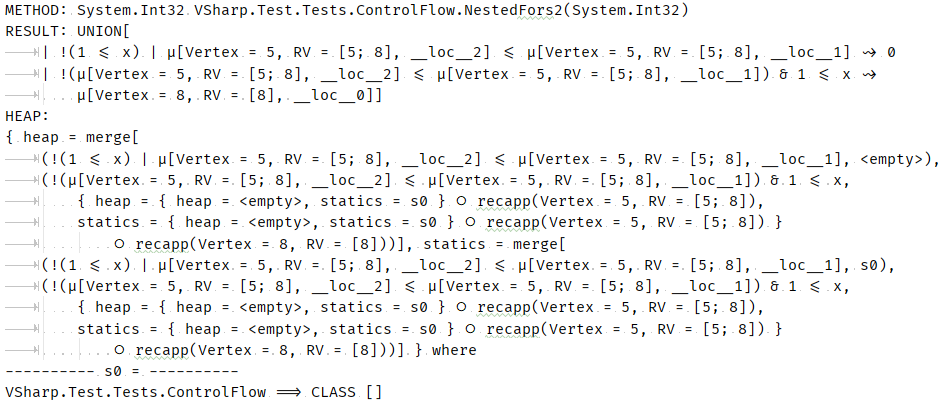
\includegraphics[scale=0.5]{Batoev/images/results.PNG}
\caption{Результат символьного исполнения метода~\ref{example:fors}}
\end{figure}

\begin{table}[t]
    \centering
    \begin{tabular}{ |p{3cm}||p{2cm}|p{2cm}|p{2cm}|  }
        \hline
        \multicolumn{4}{|c|}{Количественные характеристики тестов} \\
        \hline
        Название тестового набора &Количество тестов в наборе&Количество успешно пройденных тестов&Количество инструкций CIL\\
        \hline
        Arithmetics   &80    &77    &1968\\
        Logics        &75    &75    &1458\\
        Conditional   &10    &6     &943\\
        Recursive     &5     &5     &751\\
        Lambdas       &2     &2     &404\\
        Generic       &14    &14    &194\\
        Strings       &15    &15    &219\\
        Unsafe        &16    &16    &312\\
        Typecast      &19    &19    &969\\
        Methods       &10    &10    &238\\
        Lists         &9     &9     &1420\\
        Chess.NET     &1     &1     &2723\\
        \hline
        Всего         &256   &249   &11599\\
        \hline
    \end{tabular}
    \captionof{table}{Результаты тестирования}
    \label{experiments}
\end{table}


\FloatBarrier

\subsection{Тестирование интерпретатора}
Тестирование нового интерпретатора проводилось на тестовой подсистеме проекта <<VSharp.Test>> и на библиотеке \textsc{Chess.NET}.
Подсистема содержит тестовые наборы, затрагивающие различные конструкции и возможности языка C\#:
арифметику, логические операции,
работу с массивами разных размерностей, генерирование исключений, тесты на классы и структуры, включающие взаимодействие со статическими членами и вызовы виртуальных методов,
тесты с неограниченной рекурсией, тесты с \emph{unsafe}-кодом, тесты со строками. 

Таблица~\ref{experiments} показывает результаты проведенного тестирования. 
В наборах тестах с арифметикой и условными конструкциями была часть тестов с генерацией исключений. 
Поскольку схема обработки исключений для языка CIL не была реализована, то данные тесты были некорректно исполнены.
По той же причине не было проведено тестирования на тестовым наборе <<TryCatch>>, 
основное предназначение которого --- инициирование и перехват исключений.

\section{Заключение}

В данной работе описан подход к композициональному символьному исполнению без раскрутки. Была предложена концепция композициональной памяти с символьной адресацией. Был доказан некоторый набор свойств КСП, дающий основание для подхода в стиле систем переписывания, где символьные кучи могут сами выступать как символы. Это даёт возможность автоматически порождать уравнения на состояния, решения которых в точности отражают поведения функций, работающих с динамической памятью. Было показано как свести задачу решения уравнений на состояния к задаче проверки безопасности чистых функций второго порядка.

Данная работа нацелена на теоретические основания композиционального анализа динамической памяти. Мы оставляем апробацию этого подхода на будущее. Другим направлением будущих исследований может быть расширение нашего формализма на композициональный анализ параллельных программ.

\bibliographystyle{ugost2008ls}
\begin{thebibliography}{10}

\bibitem{baldoni2018survey}
Roberto Baldoni, Emilio Coppa, Daniele~Cono D’elia, Camil Demetrescu, and
  Irene Finocchi.
\newblock A survey of symbolic execution techniques.
\newblock {\em ACM Computing Surveys (CSUR)}, 51(3):50, 2018.

\bibitem{godefroid2007compositional}
Patrice Godefroid.
\newblock Compositional dynamic test generation.
\newblock In {\em ACM Sigplan Notices}, volume~42, pages 47--54. ACM, 2007.

\bibitem{jaffar2012tracer}
Joxan Jaffar, Vijayaraghavan Murali, Jorge~A Navas, and Andrew~E Santosa.
\newblock Tracer: A symbolic execution tool for verification.
\newblock In {\em International Conference on Computer Aided Verification},
  pages 758--766. Springer, 2012.

\bibitem{king1976symbolic}
James~C King.
\newblock Symbolic execution and program testing.
\newblock {\em Communications of the ACM}, 19(7):385--394, 1976.

\bibitem{kuznetsov2012efficient}
Volodymyr Kuznetsov, Johannes Kinder, Stefan Bucur, and George Candea.
\newblock Efficient state merging in symbolic execution.
\newblock {\em Acm Sigplan Notices}, 47(6):193--204, 2012.

\bibitem{mcmillan2010lazy}
Kenneth~L McMillan.
\newblock Lazy annotation for program testing and verification.
\newblock In {\em International Conference on Computer Aided Verification},
  pages 104--118. Springer, 2010.

\bibitem{kostyukov2018csewu}
Юрий~Олегович Костюков.
\newblock {\em Кучи как чистые функции:
  композициональное символьное исполнение
  без раскрутки}, pages 288--346.
\newblock 6. 2018.

\end{thebibliography}

\title{Композициональное символьное исполнение CIL-кода}

\titlerunning{Композициональное символьное исполнение CIL-кода}

\author{Батоев Константин Аланович}

\authorrunning{К.~А.~ Батоев}

\tocauthor{Константин Батоев}
\institute{St Petersburg State University\\
	\email{konstantin.batoev@gmail.com}}

\maketitle

% \renewcommand{\ttdefault}{cmtt}

\newsavebox\CBox
\newcommand\hcancel[2][0.1pt]{%
  \ifmmode\sbox\CBox{$#2$}\else\sbox\CBox{#2}\fi%
  \makebox[0pt][l]{\usebox\CBox}%
  \textcolor{red}{\rule[0.3\ht\CBox-#1/2]{\wd\CBox}{#1}}}

\captionsetup[figure]{name=Рисунок}

% \newtheorem*{proof}{Доказательство}

\renewcommand{\defnautorefname}{опр.}
\renewcommand{\lemautorefname}{лемм.}
\renewcommand{\remkautorefname}{зам.}
\renewcommand{\propautorefname}{св.}
\renewcommand{\exmpautorefname}{пр.}
\renewcommand{\thmautorefname}{теор.}
% \renewcommand{\crlrautorefname}{Corollary}
\renewcommand{\sectionautorefname}{разд.}
\newcommand{\algorithmautorefname}{лист.}
\newcommand{\algorithmcfname}{Листинг}
\makeatletter
\renewcommand{\ALG@name}{Листинг}
\makeatother

\algrenewcommand\alglinenumber[1]{\tiny #1:}

\lstdefinelanguage{Demo}
{
 morecomment = [l]{//}, 
 sensitive = true,
 morekeywords = {type, new, null,
   bool, int, write, read,
   fail, nop, let, alloc, in,
   if, then, else, call,
   true, false, and, or, not}
}

\definecolor{commentgreen}{RGB}{0,200,100}
\lstdefinestyle{demolang}{language=Demo,
    rulecolor=\color{blue!80!black},
    basicstyle=\ttfamily\footnotesize,
    keywordstyle=\color{blue}\ttfamily,
    stringstyle=\color{red}\ttfamily,
    commentstyle=\color{commentgreen}\ttfamily,
    numbers=left,
    numbersep=5pt,
    numberstyle=\tiny\color{black},
    escapechar=@,
    tabsize=2
}

\usemintedstyle{vs}

\counterwithin{lstlisting}{section}
\counterwithin{algocf}{section}

\fontfamily{times}
% \fontsize{10pt}{30pt}
\selectfont
\setlength{\parindent}{0em}
% \setlength{\parskip}{1em}
\renewcommand{\baselinestretch}{1.0}

\SetupFloatingEnvironment{listing}{name=Листинг}
\providecommand*{\listingautorefname}{лист.}
\renewcommand*{\figureautorefname}{рис.}
\renewcommand*{\tableautorefname}{табл.}
\SetAlgorithmName{Листинг}{лист.} 

\theoremstyle{plain}
\newtheorem{thm}{Теорема}%[section]
\newtheorem{lem}{Лемма}%[section]
% \newtheorem{crlr}{Corollary}%[section]

\theoremstyle{definition}
\newtheorem{defn}{Определение}
\newtheorem{remk}{Замечание}
\newtheorem*{remk*}{Замечание}
\newtheorem{prop}{Утверждение}
\newtheorem{exmp}{Пример}
% \newtheorem*{proof}{Доказательство}

% \newcommand{\defnautorefname}{опр.}
\newcommand{\lemautorefname}{лем.}
\newcommand{\remkautorefname}{зам.}
\newcommand{\propautorefname}{утв.}
\newcommand{\exmpautorefname}{пример}
\newcommand{\thmautorefname}{теор.}
% \renewcommand{\crlrautorefname}{Corollary}
\renewcommand{\sectionautorefname}{секция}
% \renewcommand{\algorithmautorefname}{Алгоритм}
% \renewcommand{\algorithmcfname}{Алгоритм}

% \renewcommand*{\Authsep}{\authorcr}
% \renewcommand*{\Authand}{\authorcr}
% \renewcommand*{\Authands}{\authorcr}

% \makeatletter
% \makeatother

\lstdefinelanguage{Demo}
{
 morecomment = [l]{//}, 
 sensitive = true,
 morekeywords = {new, null,
   fail, goto, halt,
   true, false, and, or, not}
}

\definecolor{commentgreen}{RGB}{0,200,100}
\lstdefinestyle{demolang}{language=Demo,
    rulecolor=\color{blue!80!black},
    basicstyle=\ttfamily\footnotesize,
    keywordstyle=\color{blue}\ttfamily,
    stringstyle=\color{red}\ttfamily,
    commentstyle=\color{commentgreen}\ttfamily,
    numbers=left,
    numbersep=5pt,
    numberstyle=\tiny\color{black},
    escapechar=@,
    tabsize=2
}

%%% For graph drawing
\definecolor {processblue}{cmyk}{0.96,0,0,0}
\definecolor {processgreen}{cmyk}{1,0,1,0}
\definecolor {processred}{cmyk}{0, 0.84, 0.80, 0.19}
\definecolor {processyellow}{cmyk}{0, 0, 1, 0}


%\newcommand{\csharp}[1]{\mintinline{csharp}{#1}}

\newcommand{\pex}{\textsc{Pex}}
\newcommand{\predator}{\textsc{Predator}}
\newcommand{\dotnet}{\textsc{.NET}}
\newcommand{\clang}{\textsc{C}}
\newcommand{\vsharp}{\textsc{V\#}}

\newcommand\addrset{loc}
\newcommand\termset{term}
\newcommand\guardset{guard}

\newcommand\eqby[1]{\mathrel{\stackrel{\mbox{\normalfont\tiny #1}}{=}}}
\newcommand\eqdef{\eqby{def}}

\newcommand\aite{ite}
\newcommand\ite[3]{\aite(#1,#2,#3)}
\newcommand\Ite[3]{\aite\big(#1,#2,#3\big)}
\newcommand\pair[2]{\langle#1, #2\rangle}
\newcommand\paiR[2]{\big\langle#1, #2\big\rangle}
\newcommand\mg[2]{#1=#2}
\newcommand\nmg[2]{#1\neq#2}
\newcommand\li[1]{LI(#1)}
\let\emptyheap\varepsilon
\newcommand\agrec{Rec}
\newcommand\agmerge{Merge}
\newcommand\agcompose{\bigcirc}
\newcommand\GRec[1]{\agrec\big(#1\big)}
\newcommand\GMerge[1]{\agmerge\big(#1\big)}
\newcommand\GCompose[2]{#1\agcompose#2}
\newcommand\agho{App}
\newcommand\gapp[1]{\agho(#1)}
\newcommand\GApp[1]{\agho\big(#1\big)}
\newcommand\aunion{\texttt{UNION}}
\newcommand\union[1]{\aunion\big(#1\big)}
\newcommand\Union[1]{\aunion\Big(#1\Big)}
\newcommand\aderef{readStore}
\newcommand\readTerm{readTerm}
\newcommand\writeTerm{writeTerm}
\newcommand\afind{find}
\newcommand\find[5]{\afind(#1,#2,#3,#4,#5)}
\newcommand\finD[5]{\afind\big(#1,#2,#3,#4,#5\big)}
\newcommand\Find[5]{\afind\Big(#1,#2,#3,#4,#5\Big)}
\newcommand\deref[2]{\aderef(#1,#2)}
\newcommand\Deref[2]{\aderef\big(#1,#2\big)}
\newcommand\compose[2]{#1\circ#2}
\newcommand\lmbd[2]{\lambda #1.#2}
\newcommand\lmbdx[1]{\lambda x.#1}
\newcommand\dom[1]{dom(#1)}
\newcommand\Dom[1]{dom\big(#1\big)}

\newcommand\Li[1]{LI\big(#1\big)}
\newcommand\amutate{writeStore}
\newcommand\amutateStack{writeStack}
\newcommand\mutate[3]{\amutate(#1,#2,#3)}
\newcommand\mutateStack[4]{\amutateStack(#1,#2,#3,#4)}
\newcommand\rdbodyext[6]{\Union{\big\{\paiR{#4\mg{#1}{#5}}{#6\big(#2(#5), xs\big)} \mid #5\in\dom{#2} \big\}\\&\qquad\qquad\qquad\cup\paiR{#4\bigwedge_{\mathclap{#5\in\dom{#2}}}{\nmg{#1}{#5}}}{#6\big(#3, xs\big)}}}
\newcommand\rdbody[4]{\rdbodyext{#1}{#2}{#3}{}{l}{#4}}
\newcommand\wrtbody[6]{\Union{&\paiR{\mg{#1}{#2}}{\writeTerm\big(#3,#4,#6\big)},
    \\&\paiR{\nmg{#1}{#2}}{\writeTerm\big(#5(#1),#4,#6\big)}}}
\newcommand{\var}[1]{\mathit{#1}}


\begin{abstract}
Известно, что наибольшую сложность в области верификации программ представляет задача доказательства корректности программ с циклическими участками кода. Опираясь на подход символьного исполнения программ и на введенные формализмы обобщённых куч в работе~\cite{kostyukov2018csewu}, данная работа представляет алгоритм композиционального символьного исполнения без раскрутки отношения перехода программ с произвольным графом потока управления. На его основе был реализован символьный интерпретатор языка CIL в проекте V\#, символьной виртуальной машине для анализа .NET. Была проведена апробация алгоритма на примерах, включающих сложные потоки управления, и интерпретатора на тестовой базе проекта VSharp.Test и на библиотеке Chess.NET.
\end{abstract}
\section*{Введение}
Поиск путей в графе с ограничением в виде формальных языков~\cite{FLCpathProblem} --- это задача, в которой формальные языки используются для задания множества искомых путей. В таком подходе каждый путь соответствует слову, состоящему из меток его рёбер, а ограничением на путь является принадлежность соответствующего ему слова некоторому заданному формальному языку.

В качестве класса формальных языков по иерархии Хомского наибольший интерес представляют контекстно-свободные языки. В отличие от регулярных они обладают большей выразительностью. Поэтому в задаче поиска путей контекстно-свободные ограничения позволяют задавать более сложные отношения между вершинами. Так, например, важный класс запросов поиска вершин, лежащих на одном уровне иерархии~\cite{zhlang-2016}, задаётся только контекстно-свободными, но не регулярными ограничениями. Запросы такого вида, как и другие запросы с контекстно-свободными ограничениями имеют широкое применение в биоинформатике~\cite{bio-application} и при обработке rdf-файлов~\cite{zhlang-2016}.

Наиболее удобным и подходящим инструментом для работы с граф\-структурированными данными являются графовые базы данных. Так же как и реляционные, графовые базы данных поддерживают свой язык запросов. С его помощью графовые базы данных позволяют решать вышеупомянутую задачу поиска путей. Но ограничения на пути, которые поддерживается в наиболее распространённых базах данных, являются в лучшем случае регулярными.

Отсутствие поддержки контекстно-свободных ограничений в графовых базах данных, во-первых, сильно ограничивает выразительность языка запросов. Во-вторых, при необходимости в более сложных запросах разработчикам приходится самим писать алгоритмы, решающие задачу контекстно-свободной достижимости для их частного случая. Так, например, Хуэй Мяо и др.~\cite{datascince-lifecycle} разработали систему хранения и отслеживания версий артефактов, возникающих при научных работах. Вся информация про артефакты хранилась в графовой базе данных. При этом при разработке возникла потребность в выполнении запросов с контекстно-свободными ограничениями для выявления взаимоотношений между различными версиями различных артефактов. Это и послужило началом статьи~\cite{datascince-lifecycle}, в которой приводятся алгоритмы решения частных запросов.

В недавнем исследовании Йохем Куйперс и др.~\cite{Kuijpers:2019:ESC:3335783.3335791} произвели сравнительный анализ наиболее известных алгоритмов поиска путей с конте\-кстно-свободными ограничениями. Алгоритмы запускались на графах, находящихся в хранилище графовой базы данных Neo4j. По результатам исследования было показано, что в контексте Neo4j алгоритмы обладают большим временем работы, и поэтому дальнейшая работа по расширению языка запросов прекратилась. При этом Рустам Азимов~\cite{Azimov:2018:CPQ:3210259.3210264} предоставил матричный алгоритм и его реализацию, которая работает за разумное время на реальных данных. Но, так как алгоритм был реализован вне контекста базы данных, его результат приняли недостаточно показательным. Поэтому вопрос о реализуемости запросов с контекстно-свободными ограничениями в графовых базах данных, а соответственно и о возможности расширения языка запросов для их поддержки остаётся открытым.

\section{Постановка задачи}
Целью данной работы является полная поддержка запросов с конте\-кстно-свободными ограничениями для графовой базы данных. А именно, необходимо предоставить пользователю возможность формулировать запросы с контекстно-свободными ограничениями в терминах одного из существующих стандартных языков запросов и исполнять их в графовой базе данных за приемлемое время. Для достижения этой цели были поставлены следующие задачи.

\begin{itemize}
    \item Выполнить обзор существующих реализаций поддержки запросов с контекстно-свободными ограничениями в графовых базах данных. В результате обзора необходимо выбрать наиболее перспективный с точки зрения производительности алгоритм решения задачи контекстно-свободной достижимости и подходящую для его интеграции базу данных. При выборе базы данных необходимо учитывать как возможность интеграции выбранного алгоритма, так и возможность поддержки одного из стандартных языков запросов, позволяющего выражать контекстно-свободные ограничения.
    \item Интегрировать выбранный на предыдущем шаге алгоритм в выбранную графовую базу данных.
    \item Расширить язык запросов выбранной базы данных конструкциями, необходимыми для выражения контекстно-свободных ограничений.
    \item Произвести замеры производительности полученного решения и сравнить его с существующими решениями.
\end{itemize}


\section{Обзор}

\subsection{Терминология}
Контекстно-свободной грамматикой называется $G = (\Sigma, N, P, S)$, где $\Sigma$ --- алфавит терминальных символов, $N$ --- алфавит нетерминальных символов, $P$ --- множество правил вида $A \rightarrow \alpha$, где $A \in N$, $\alpha \in (\Sigma \cup N)^*$, а $S \in N$ --- выделенный стартовый нетерминал.

% \gsv{про S забыли}.

Языком $L$ над алфавитом $\Sigma$ называется любое подмножество $2^{\Sigma^*}$. Языком, порождаемой грамматикой G, является множество $L(G) = \{S \xRightarrow{*} \beta, \beta \in \Sigma^*\}$, где $S \xRightarrow{*} \beta$ означает, что из нетереминала $S$ путём последовательного применения правил грамматики выводится $\beta$.

Контекстно-свободная грамматика $G = (\Sigma, N, P, S)$ находится в осла\-бленной нормальной форме Хомского, если любое её правило имеет вид $A \rightarrow BC$, где $A, B, C \in N$, либо $A \rightarrow a$, где $A \in N, a \in \Sigma$. В отличие от нормальной формы Хомского в ослабленной, во-первых, допускается присутствие стартового нетерминала $S$ в правых частях правил грамматики, во-вторых, запрещаются правила вида $S \rightarrow \epsilon$, где $\epsilon$ --- пустая строка.

% \gsv{Это не нормальная форма Хомского. У НФХ есть дополнительные ограничения. Мы называем то, что здесь, ослабленной НФХ. Важно отдельно проговорить разницу с НФХ.}

В задаче поиска путей с ограничениями в виде формальных языков дан граф $(V, E)$, разметка его рёбер $l: E \rightarrow \Sigma$ и язык $L$ над алфавитом $\Sigma$. Требуется найти множество всех пар вершин, между которыми существует путь, метки на рёбрах которого образуют слово в заданном языке. То есть требуется найти следующее множество:
\[\{(v, to): \exists p=(e_1,...,e_n) \in E^*: l(e_1)...l(e_n) \in L,~src(e_1)=v,~dst(e_n)=to\}\]
Здесь $src(e)$ и $dst(e)$ для $e \in E$ означают начальную и конечную вершину ребра $e$. В данном контексте язык $L$ называется языком ограничений.
% \gsv{У Вас вершины v и to никак с путём не связаны}

Задача поиска путей с контекстно-свободными ограничениями --- это задача поиска путей в виде формальных языков, в которой язык задаётся контекстно-свободной грамматикой.

\subsection{Графовые базы данных}
Графовые СУБД\footnote{СУБД --- Система управления базами данных} (далее просто графовые базы данных) --- это разновидность СУБД, в которой данные хранятся в виде графов. В отличие от других разновидностей, в графовых базах данных отношения между объектами так же важны, как и сами объекты.

Основной моделью представления графов в таких базах данных является gpraph property model~\cite{graph-propery-model}. В ней каждая сущность может содержать набор свойств в формате ключ-значение. Основными сущностями являются узлы и отношения. Узлы соответствуют вершинам графа и помимо свойств могут иметь несколько меток. Отношения соответствуют рёбрам и имеют ровно одну метку, которая называется типом отношения. На рисунке~\ref{fig:graph_bd_1} показан небольшой пример графа в такой модели. 

\begin{figure}[h]
\centering
    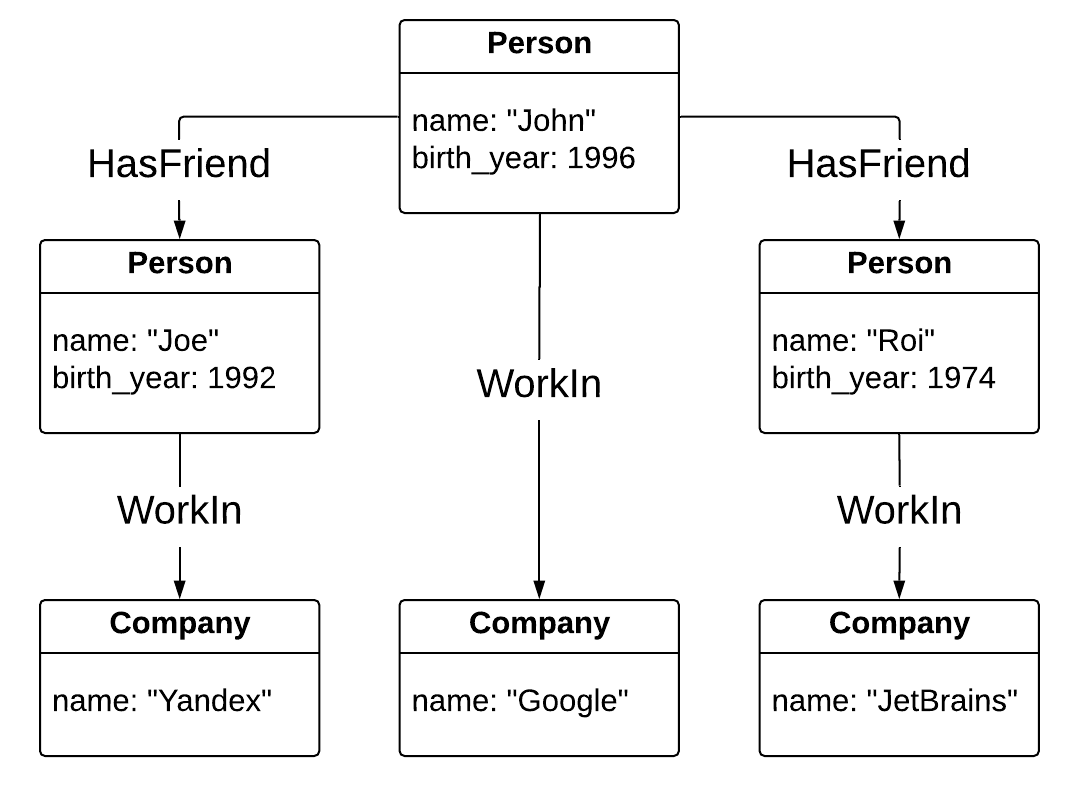
\includegraphics[width=0.7\linewidth]{Terekhov/pictures/graph_bd_1.png}
    \caption{Пример социального графа}
    \label{fig:graph_bd_1}
\end{figure}

Для работы с графами графовые базы данных предоставляют язык запросов, самым популярным из которых является Cypher~\cite{cypher-language}. В нём главный интерес представляют запросы вида сопоставления с образцом. Они позволяют задавать интересующие пути или подграфы в виде шаблонов и описывать информацию, которую нужно извлечь после удачного сопоставления. На рисунке~\ref{code:cypher_query} приведён пример такого запроса. Шаблон пути описывается в выражении MATCH. В нём между круглыми скобками задаются шаблоны вершин, а между квадратными шаблоны рёбер. Таким образом в данном примере задаются следующие ограничения: путь должен начинаться из вершины с меткой Person и именем John и состоять из двух рёбер, первое из которых должно иметь тип HasFriend, а второе WorkIn. В выражении RETURN задаётся информация, которую нужно извлечь. В данном примере это имя последней в пути вершины. В итоге ответом на такой запрос являются имена компаний, в которых работают друзья Джона. Результатом работы этого запроса на графе из рисунка~\ref{fig:graph_bd_1} является множество \{"Yandex", "JetBrains"\}.

%\lstset{
%   basicstyle=\fontsize{14}{14}\selectfont\ttfamily
%}

\begin{figure}[h]
\begin{lstlisting}[language=sql]
MATCH (p:Person)-[:HasFriend]->()-[:WorkIn]->(to)
WHERE p.name = "John"
RETURN to.name
\end{lstlisting}
\caption{Пример конечного запроса на языке Cypher}
\label{code:cypher_query}
\end{figure}

С формальной точки зрения шаблоны пути в выражении MATCH позволяют поставить задачу поиска путей с ограничениями в виде формальных языков. Так в запросе на рисунке~\ref{code:cypher_query} языком ограничений является конечный язык $\{(HasFriend, WorkIn)\}$. Для запроса на рисунке~\ref{code:cypher_query_2} ограничением является регулярный язык $\{A, B\}^*$. 

\begin{figure}[h]
\begin{lstlisting}[language=sql]
MATCH (v)-[:A | :B *]->(to)
RETURN to.name
\end{lstlisting}
\caption{Пример регулярного запроса на языке Cypher}
\label{code:cypher_query_2}
\end{figure}

При этом регулярные ограничения поддерживаются лишь частично и позволяют искать только пути произвольной длины с заданными метками на рёбрах, а более глубокие регулярные выражения не поддерживаются. Поэтому на текущий момент язык запросов довольно ограничен.

\subsection{Существующие решения}
Как было упомянуто раннее, ни одна графовая база данных не поддерживает запросов с контекстно-свободными ограничениями. Тем не менее существуют альтернативные решения поддержки таких запросов. 

\subsubsection{Парсер-комбинаторы для Neo4j}\label{sec:pareser-combinators}
В 2018 году группой исследователей из JetBrains Research на основе библиотеки Meerkat была разработана библиотека для поддержки запросов с контекстно-свободными ограничениями~\cite{parser-combinators}. Она использует графовую базу данных Neo4j~\cite{neo4j} как хранилище графов и позволяет задавать запросы в виде парсер-комбинаторов. Основным достоинством данной работы является то, что с помощью этой библиотеки кроме контекстно-свободных запросов можно выразить базовую часть языка Cypher. Но так как конкурировать с оригинальной реализацией выполнения запросов Neo4j очень сложно, это достигается вместе c сильной потерей производительности. Кроме этого контекстно-свободные запросы обрабатываются также достаточно медленно.

Таким образом данное решение является альтернативой языка запросов Neo4j, а не его расширением. Из-за медленного времени работы такое решение подходит только для работы с небольшими графами. 

\subsubsection{Расширение языка запросов SPARQL}\label{subsection:cypher-extention-2}
%Про sparql%
В 2016 Сяованг Чжан предоставил язык cfSPARQL~\cite{zhlang-2016} --- расширение языка SPARQL, который способен выразить запросы с контекстно-свободными ограничениями. Также он привёл алгоритм для вычисления таких запросов и замеры производительности. Но, во-первых, работа была сделана вне контекста графовой базы данных, а во-вторых, время работы предложенного алгоритма было больше, чем время работы парсер-комбинаторов.

\subsubsection{Существующие реализации алгоритмов решения задачи контекстно-свободной достижимости}
Основной сложностью расширения языка запросов для поддержки запросов с контекстно-свободными ограничениями является долгое время работы соответствующих алгоритмов. Так, например, в 2019 году Йохем Куйперс и другие исследователи с целью попытки расширения языка запросов Cypher для графовой базы данных Neo4j произвели сравнительный анализ производительности наиболее известных алгоритмов решения задачи контекстно-свободной достижимости.

В данном исследовании были рассмотрены и произведены замеры времени работы алгоритма Элле Хелингса~\cite{hellings-2015}, основанного на атрибутных грамматиках, восходящего алгоритма Фреда Сантоса~\cite{santos-2018}, матричного алгоритма Рустама Азимова~\cite{Azimov:2018:CPQ:3210259.3210264} и алгоритма Петтери Севона~\cite{bio-application}. Все алгоритмы были интегрированы в Neo4j и запускались на графах, находящихся в её хранилище. Алгоритмы были написаны на языке Java, при этом их реализация являлась однопоточной.

% \gsv{В таких местах надо сразу ссылку на алгоритм давать.}

По результатам замеров производительности было показано, что время работы алгоритмов является слишком большим и неприемлемым для широкого практического использования. Поэтому дальнейшая работа по интеграции и расширению языка запросов была приостановлена.

Тем не менее, матричный алгоритм Рустама Азимова в сравнительном анализе Йохема Куйперса был реализован без необходимых матричных библиотек, которые могут сильно уменьшить время его работы. Так, например, в исследовании Никиты Мишина и др.~\cite{azimov-evalution} был произведён сравнительный анализ времени работы нескольких реализаций алгоритма Рустама Азимова, основанных на различных специализированных матричных библиотеках. Графы и запросы к ним были взяты из объемлющего набора данных CFPQ\_Data~\cite{cfpq-data}, предоставленного лабораторией языковых инструментов JetBrains Research. 

Результаты замеров Никиты Мишина и др. показали, что при грамотной реализации алгоритма Рустама Азимова и использовании подходящих матричных библиотек можно добиться очень высокой производительности. Поэтому, так как основной проблемой применимости запросов с контекстно-свободными ограничениями является долгое время работы соответствующих алгоритмов, в качестве алгоритма решения задачи конте\-кстно-свободной достижимости был выбран матричный алгоритм Рустама Азимова.

\subsection{Матричный алгоритм Рустама Азимова}\label{sec:matrix-algo}
Выбранный в предыдущей главе алгоритм Рустама Азимова~\cite{Azimov:2018:CPQ:3210259.3210264}, в отличие от других алгоритмов решения задачи контекстно-свободной достижимости~\cite{hellings-2015, santos-2018, zhlang-2016}, работает с графами в виде разреженных матриц смежности. Данный алгоритм состоит из последовательности операций над разреженными матрицами, время работы которых зависит не от размеров матричных операндов, а от количества их ненулевых элементов.

На вход алгоритму (см. алгоритм 1) поступает помеченный граф $D=(V,E)$ и контекстно-свободная грамматика $G=(\Sigma, N, P, S)$ в ослабленной нормальной форме Хомского. Для каждого нетерминала $A$ в ассоциативном массиве $T$ хранится соответствующая ему булева матрица $T[A]$. На всём этапе алгоритма поддерживается следующий инвариант: $T[A]_{i,j} = 1$ равносильно существует пути, метки на рёбрах которого образуют слово, выводящееся из нетерминала $A$. На первом этапе происходит инициализация матриц с помощью простых правил грамматики, после чего инвариант выполняется для всех путей единичной длины. На втором этапе происходит транзитивное замыкание, после чего этот инвариант верен для всех путей. Результатом данного алгоритма является матрица, соответствующая стартовому нетерминалу $S$.

%  Это позволяет для его реализации использовать многопоточные матричные библиотеки, с помощью которых можно добиться очень высокой производительности. Поэтому на текущий момент алгоритм Рустама Азимова показывает наилучшее время работы на практике.

\begin{algorithm}
\caption{Матричный алгоритм Рустама Азимова}

\begin{algorithmic}[1]
\Function{contextFreePathQuerying}{$D$, $G$}
    \State{$n =$ getNodeCount(D)}
    \State{$N =$ getAllNonterms(G)}
    \State{$E =$ getEdges($D$)}
    \State{$P =$ getRules($G$)}
    \State{$S =$ getStartNonterm($G$)}
    \State{$T = \{A \rightarrow \varnothing_{n \times n} : A \in$ $N$ \} }
    \ForAll{$(v, to, label) \in E$}
    \Comment{Инициализация матриц}
        \ForAll{$A \rightarrow label \in P$}
            \State{$T[A]_{i,j} = 1$}
        \EndFor
    \EndFor    
    \While{$\exists A: T[A]$ is changing}
    \Comment{Вычисление замыкания}
        \ForAll{$A \rightarrow BC \in P$}
            \State{$T[A] \oplus= T[B] \otimes T[C]$}
        \EndFor
    \EndWhile
\State \Return $T[S]$
\EndFunction

\end{algorithmic}
\end{algorithm}

Практическое время работы алгоритма Рустама Азимова сильно зависит от производительности используемой матричной библиотеки. Это накладывает некоторые ограничения на выбор подходящей графовой базы данных, так же как и возможность представления графов в матричном виде.

\subsection{RedisGraph}
RedisGraph~\cite{redis-graph} --- это высокопроизводительная графовая база данных, поддерживающая язык запросов Cypher. В отличие от наиболее распространённой графовой базы данных Neo4j~\cite{neo4j}, RedisGraph написан на языке Си и для работы с данными использует Redis~\cite{redis}, основным достоинством которого является возможность хранить данные прямо в оперативной памяти. Это позволяет RedisGraph быстро обрабатывать пользовательские запросы.

Также RedisGraph является единственной графовой базой данных, которая работает с графами в виде разреженных матриц смежности и транслирует запросы языка Cypher в матричные выражения. Для представления графов в таком виде и работы с ними в терминах линейной алгебры используется мощный матричный фреймворк GraphBlas~\cite{graph-blas}. Его реализация SuiteSparse~\cite{suite-sparse} является многопоточной и сильно оптимизирована, что позволяет RedisGraph добиться высокой производительности.

Из всего этого следует, что RedisGraph идеально подходит для интеграции матричного алгоритма. Во-первых, графы представляются в необходимом алгоритму виде, что позволит избежать издержек на конвертацию форматов. Во-вторых, использование SuiteSparse для вычисления матричных операций позволит добиться высокой производительности. Поэтому RedisGraph был выбран в качестве графовой базы данных для интеграции матричного алгоритма и расширения языка запросов.

% Так как алгоритм Рустама Азимова работает с матричным представлением графа,, как наиболее подходящий для интеграции матричного алгоритма.

\subsection{Расширение языка Cypher}\label{subsection:cypher-extention}
На текущий момент оригинальная версия языка Cypher, используемая в том числе и в RedisGraph, не поддерживает запросов с контекстно-свободными ограничениями. Но тем не менее в 2017 году был разработан черновой вариант спецификации расширения Cypher~\cite{cypher-specification}, которая вводит в язык шаблоны путей. Они позволяют выразить более сложные запросы, в том числе запросы с контекстно-свободными ограничениями.

Шаблоны путей являются альтернативой шаблонам рёбер, которые есть в оригинальном Cypher. Они, как и шаблоны рёбер, могут встречаться в выражении MATCH и иметь своё направление. Кроме этого в глобальной области запроса им можно задавать имя, на которое потом можно ссылаться внутри других шаблонов.

Шаблон пути представляет из себя регулярное выражение над некоторыми примитивами. В качестве таких примитивов могут выступать шаблоны рёбер, шаблоны вершин и ссылки на именованные шаблоны путей. Также любым подвыражениям можно задавать своё направление. Основная часть конкретного синтаксиса данного расширения приведена на рисунке~\ref{fig:cypher_syntax}.

\begin{figure}[]
\begin{align*}
\begin{split}
PathPattern     &= ["<"],~"-/",~PathExpression,~"/-",~[">"]\\
PathExpression  &= \{PathAlternative\}\\
PathAlternative &= PathRepetition,~\{"|", PathRepetition\}\\
PathRepetition  &= ["<"],~PathBase,~[">"],~("*")
\end{split}\\
\begin{split}
PathBase &= PathEdge \\
         &~~|~PathNode \\
         &~~|~PathReference \\
         &~~|~"[",~PathExpression,~"]"
\end{split}\\
\begin{split}
PathEdge      &= Label \\
PathNode      &= "(",~[Label,~\{"|",~Label\}],~")" \\
PathReference &= "\sim",~SymbolicName; \\
Label         &= ":",~LabelName
\end{split}
\end{align*}
\caption{Расширение конкретного синтаксиса Cypher}
\label{fig:cypher_syntax}
\end{figure}

Каждый шаблон пути задаёт отношение на множестве вершин. Поэтому семантикой языка шаблонов путей $L_{P}$ в контексте графа $G(V, E)$ является отображение $\llbracket \cdot \rrbracket_{G}: L_P \rightarrow V \times V$, которое каждому шаблону $p\in L_P$ сопоставляет множество пар вершин, между которыми существует путь, удовлетворяющий данному шаблону $p$. 

Подробное описание данной семантики приводится в таблице~\ref{tab:cypher_sematic}.  В ней наибольший интерес представляют именованные шаблоны путей, так как именно с помощью них можно выразить запросы с контекстно-свободными ограничениями. Все именованные шаблоны путей $S_i = p_j$ можно рассматривать как правила контекстно свободной грамматики с алфавитом нетерминалов $\{S_i\}_{i=1}^n$. Тогда каждый нетерминал $S_j$ порождает язык $L_{S_j} \subset L_p$, а семантикой соответствующего именованного шаблона пути $S_j=p_j$ является множество $\bigcup\limits_{p \in L_{s_j}} \llbracket p \rrbracket_{G}$.

На рисунке~\ref{code:cypher_query_3} приведён пример запроса в расширенном синтаксисе. В нём декларируется именованный шаблон S, который задаёт множество правильных скобочных последовательностей над ребрами с типом L и R. Далее в выражении MATCH задаётся шаблон пути, состоящий из ссылки на шаблон S. Таким образом результатом обработки запроса является множество всех пар вершин, между которыми существует путь, метки на рёбрах которого образуют правильную скобочную последовательность. 

\begin{table}[h!]
\begin{adjustbox}{max width=\textwidth}
\begin{tabular}{|c|c|c|}
\hline
$p \in L_P$                                                                                  & $\llbracket p \rrbracket_{G}$                                                                                                                                                                                   & Описание шаблона пути                                                                                                         \\ \hline
\hline
()                                                                                            & $\{(v, v): v \in V\}$                                                                                                                                                                                           & \begin{tabular}[c]{@{}c@{}}Пустой путь, состоящий из \\ одной произвольной вершины\end{tabular}                               \\ \hline
:a                                                                                            & $\{e=(v,to): e \in E, type(e)=a\}$                                                                                                                                                                              & \begin{tabular}[c]{@{}c@{}}Путь единичной длины,\\  состоящий из ребра с типом $a$\end{tabular}                               \\ \hline
(:b)                                                                                          & $\{(v, v): v \in V, label(v)=b\}$                                                                                                                                                                               & \begin{tabular}[c]{@{}c@{}}Пустой путь, состоящий из одной\\  вершины, помеченной меткой $b$\end{tabular}                     \\ \hline
$\alpha~\beta$                                                                                & $\llbracket \alpha \rrbracket_{G}\circ \llbracket \beta \rrbracket_{G}$                                                                                                                                         & Конкатенация путей $\alpha$ и $\beta$                                                                                         \\ \hline
$\alpha~|~\beta$                                                                              & $\llbracket \alpha \rrbracket_{G}\cup \llbracket \beta \rrbracket_{G}$                                                                                                                                          & Альтренатива между путями $\alpha$ и $\beta$                                                                                  \\ \hline
$[\alpha]$                                                                                    & $\llbracket \alpha \rrbracket_{G}$                                                                                                                                                                              & \begin{tabular}[c]{@{}c@{}}Квадратные скобки позволяют \\ группировать  выражения \\ для задания ассоциативности\end{tabular} \\ \hline
\textless{}$\alpha$                                                                           & $\{(to, v): (v, to) \in \llbracket \alpha \rrbracket_{G}\}$                                                                                                                                                     & Путь, обратный к пути $\alpha$                                                                                                \\ \hline
\textless{}$\alpha$\textgreater{}                                                             & $\llbracket \alpha~|~$\textless{}$\alpha \rrbracket_{G} $                                                                                                                                                       & \begin{tabular}[c]{@{}c@{}}Альтернатива между путём $\alpha$ и\\ обратным к нему\end{tabular}                                 \\ \hline
$\alpha^*$                                                                                    & $\llbracket \alpha \rrbracket_{G}^{*}$                                                                                                                                                                          & \begin{tabular}[c]{@{}c@{}}Путь, состоящий из\\ конкатенации 0 или более путей $\alpha$\end{tabular}                          \\ \hline
\begin{tabular}[c]{@{}c@{}}$\{S_i = p_i\}_{i=1}^{n}$\\ -- named\\  path patterns\end{tabular} & \begin{tabular}[c]{@{}c@{}}$P = \{S_i \rightarrow p_i\}_{i=1}^n$\\ $Gram_j = (\Sigma, \{S_i\}_{i=1}^n, P, S_j)$\\ $\llbracket S_j \rrbracket_{G} = \bigcup\limits_{p \in L(G)}{\llbracket p \rrbracket_{G}}$\end{tabular} & Именнованые шалоны путей                                                                                                      \\ \hline
$\sim$$S$                                                                                     & $\llbracket S \rrbracket_{G}$                                                                                                                                                                                   & \begin{tabular}[c]{@{}c@{}}Ссылка на именнованный\\  шаблон пути\end{tabular}                                                 \\ \hline
\end{tabular}
\end{adjustbox}
\caption{Семантика языка шаблонов путей}
\label{tab:cypher_sematic}
\end{table}

\begin{figure}[h!]
\begin{lstlisting}[language=sql]
PATH PATTERN S = ()-/ [:L ~S :R] | [~S ~S] | () /-()
MATCH (v)-/ ~S /-(to)
RETURN v, to
\end{lstlisting}
\caption{Пример запроса в расширенном синтаксисе Cypher}
\label{code:cypher_query_3}
\end{figure}

Данная спецификация расширения Cypher была представлена официальными разработчиками и сильно расширяет выразительность языка, предоставляя удобную возможность выражать запросы как с регулярными, так и с контекстно-свободными ограничениями. Поэтому в моей работе приводится поддержка выполнения запросов именно для этого расширения языка.

% \gsv{Не хватает какого-то чёткого вывода про то, что вот именно это мы и буем использовать.}

\section{Реализация}
По результатам обзора было решено реализовать поддержку расширения языка Cypher, представленную в главе~\ref{subsection:cypher-extention}, для графовой базы данных RedisGraph. За основу алгоритма, решающего задачу поиска путей с контекстно-свободными ограничениями, был взят матричный алгоритм Рустама Азимова, описанный в главе~\ref{sec:matrix-algo}.

% \gsv{И зжесь надо ещё раз подитожить в духе "по результатм обзора было решено сделать то и это с использованием того и сего"}

\subsection{План выполнения запроса}\label{execution-plan}
В RedisGraph основной частью обработки запроса является построение плана его выполнения. Её часть, которая относится к шаблонам путей приведена на рисунке~\ref{fig:execution_plan}. В ней зелёным цветом выделено то, что было добавлено или расширено.

В самом начале, после получения запроса строится его абстрактное синтаксическое дерево \textit{AST}. Далее, из него извлекаются именованные и неименованные шаблоны путей \textit{PathPattern} и \textit{NamedPathPatterns}, после чего они преобразуются в более удобное промежуточное представление \textit{PathExpr}. При этом, для дальнейшего связывания ссылок, именованные шаблоны сохраняются в глобальном контексте запроса \textit{PathPatternCtx}.

На следующем этапе происходит трансляция промежуточных представлений \textit{PathExpr} в матричные выражения \textit{AlgebraicExpression}. В них операндами являются либо матрицы, полученные из указанного в запросе графа \textit{GraphCtx}, либо ссылки на именованные шаблоны путей из \textit{PathPatternCtx}. Основной идеей трансляции является то, что после вычисления матричного выражения получается матрица, которая задаёт то же самое отношение на множестве вершин, что и исходный шаблон пути.

Далее каждое такое выражение формирует новую операцию плана выполнения запроса \textit{CfpqTraverseOp}. При её вычислении сначала происходит запуск расширенной версии матричного алгоритма Рустама Азимова. Он решает задачу контекстно-свободной достижимости, заданной именованными шаблонами путей. После этого все ссылки в матричном выражении заменяются на полученные в ходе алгоритма матрицы и происходит вычисление матричного выражения. Каждая такая операция добавляется в план выполнения запроса.

%  \gsv{Используйте \textit{CfpqTraverseOp} вместо долларов для длинных слов. Они тогда не распадаются из-а лишних пробелов.}

\begin{figure}[H]
\centering
    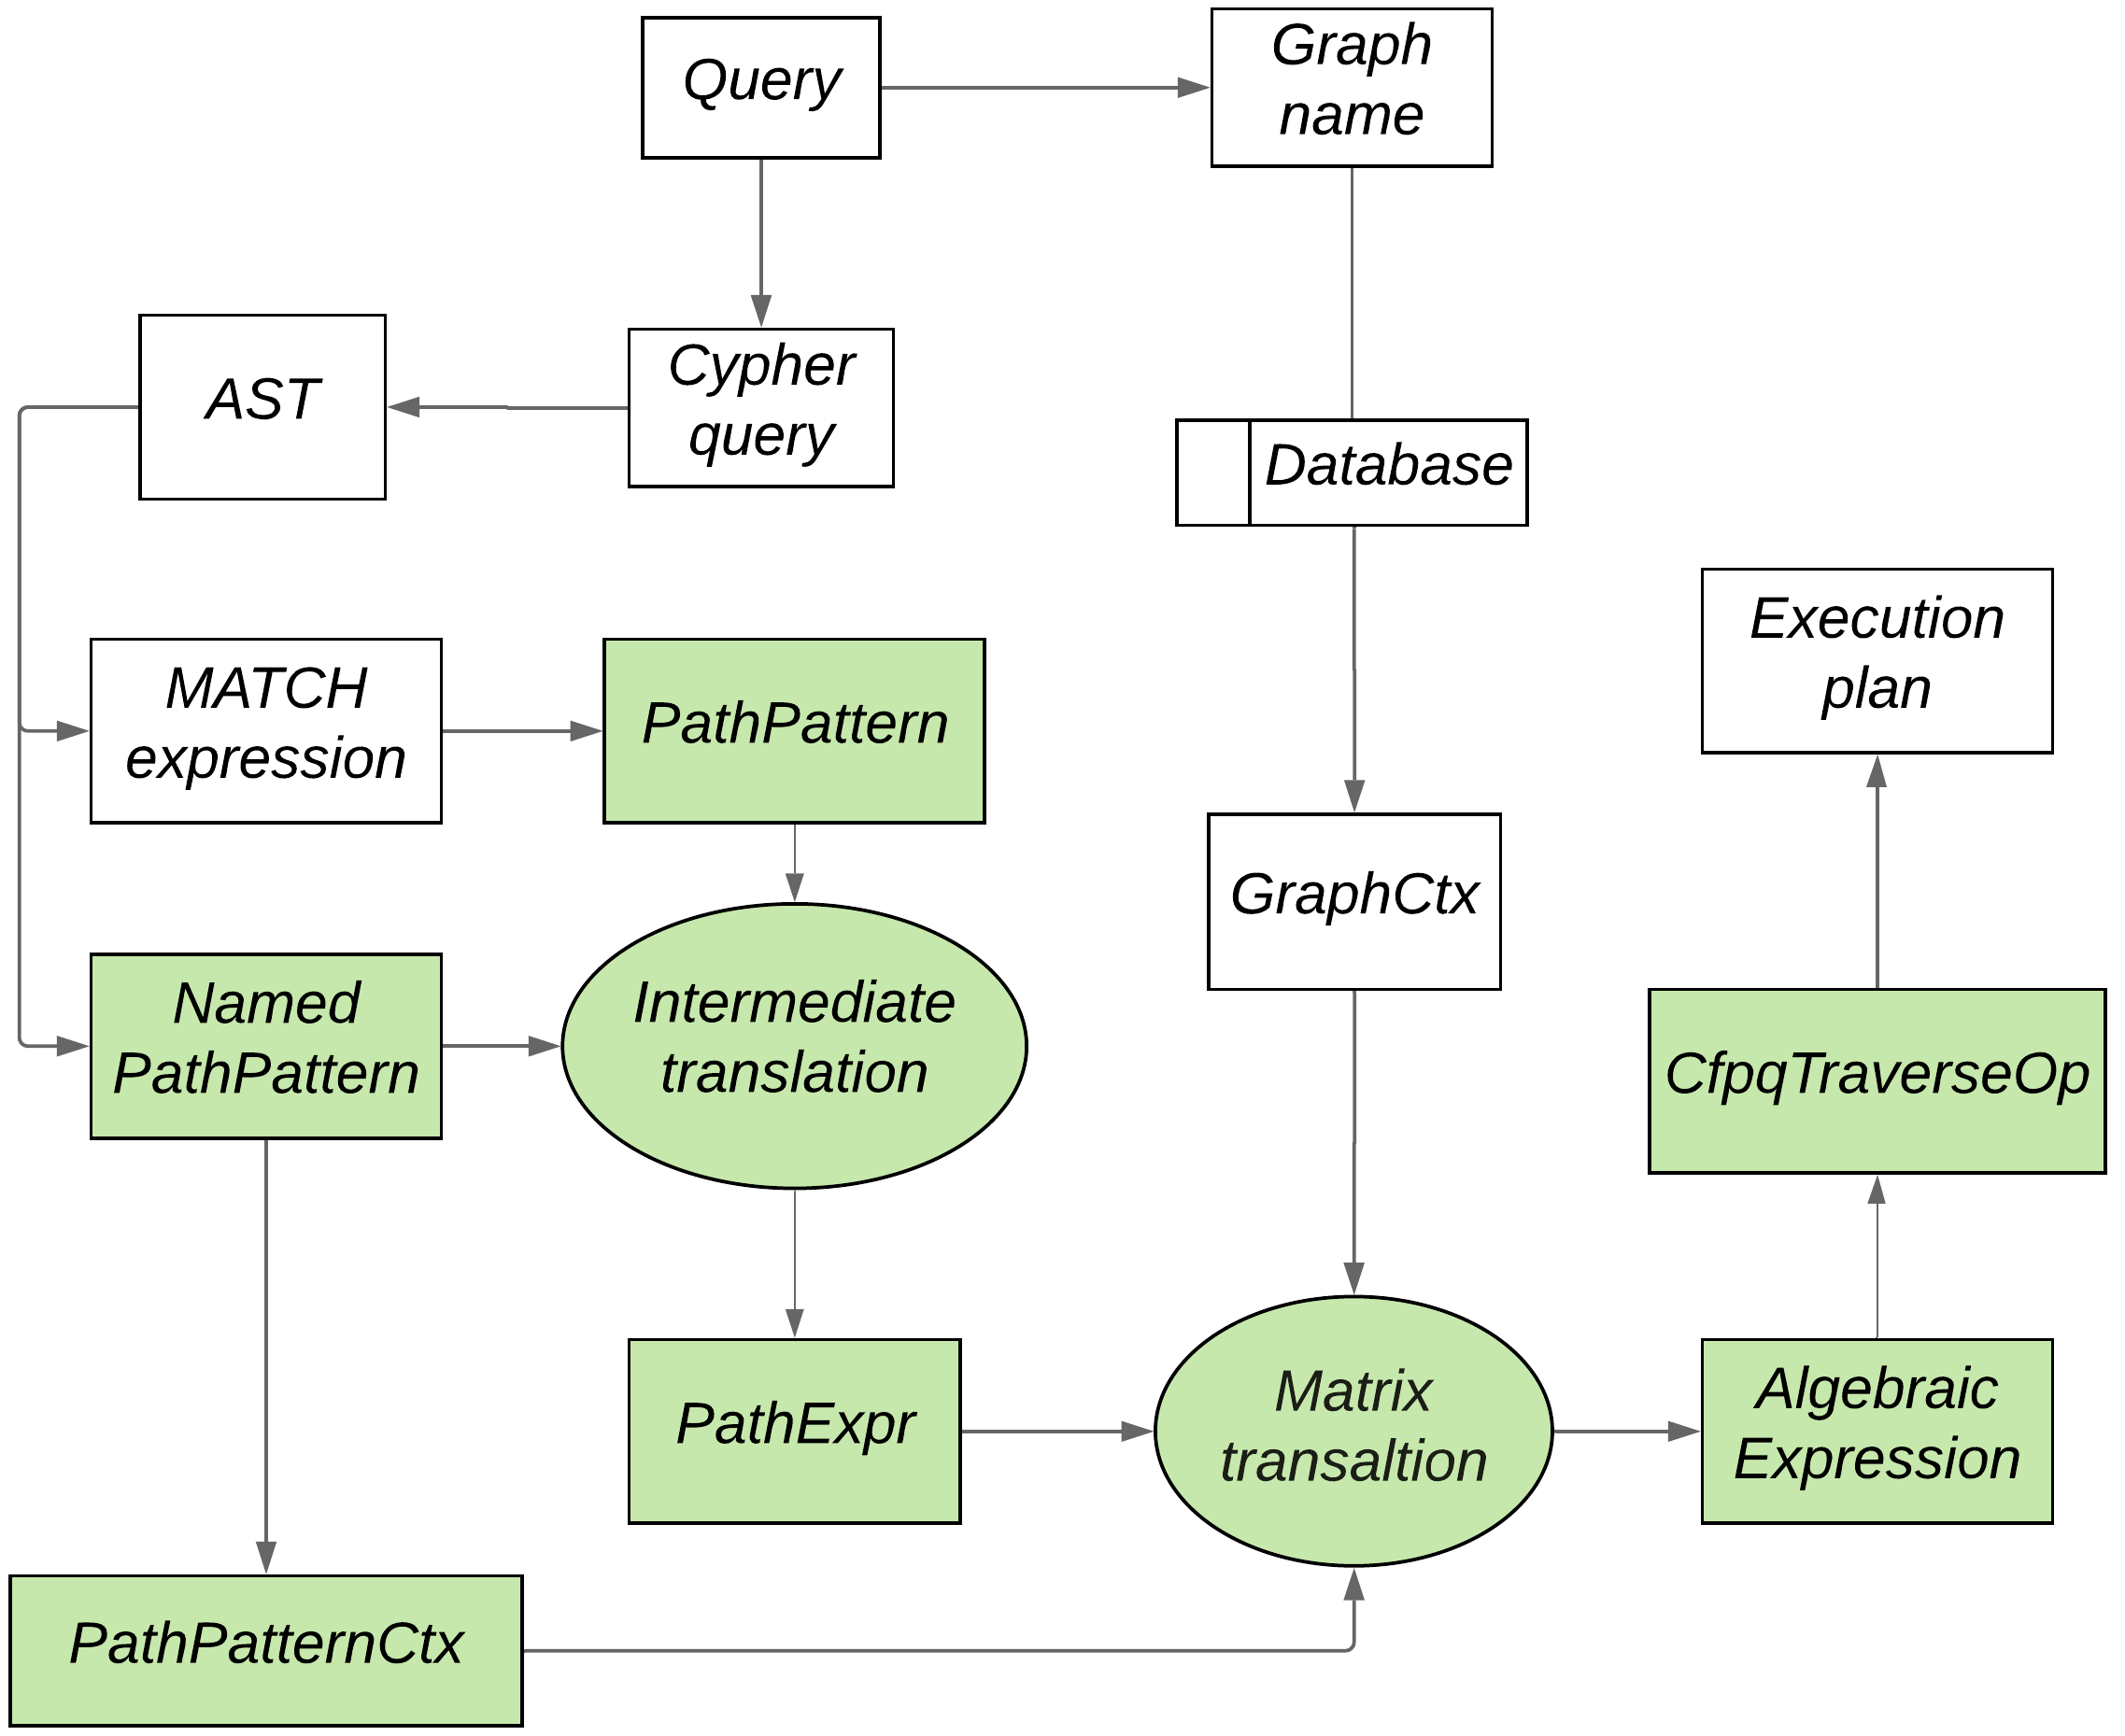
\includegraphics[width=1.0\linewidth]{Terekhov/pictures/execution_plan_3.png}
    \caption{Расширение построения плана выполнения запроса}
    \label{fig:execution_plan}
\end{figure}

\subsection{Промежуточное представление}\label{matrix-translation}
Шаблоны путей, полученные из \textit{AST}, транслируются в промежуточное представление \textit{PathExpr}. Оно позволяет задавать более простой абстрактный синтаксис, который описан на рисунке~\ref{fig:intermidiate_repr}. 

Таким образом, альтернативе и конкатенации шаблонов соответствуют \textit{PathAlt} и \textit{PathSeq}, \textit{PathGroup} позволяет задавать направление пути и наличие замыкания, а \textit{PathBasic} соответствует либо примитивным шаблонам \textit{PathNode}, \textit{PathEdge} и \textit{PathRef}, либо целому выражению \textit{PathExpr}. Примеры промежуточного представления шаблонов приведены в таблице~\ref{tab:inter_examples}.
\begin{figure}[h!]
\begin{align*}
\begin{split}
PathExpr=~ &PathSeq(PathExpr,~PathExpr)~|\\
           &PathAlt(PathExpr,~PathExpr)~|\\
           &PathGroup(PathBasic, direction, range)
\end{split}\\
\begin{split}
PathBasic=~ &PathNode(label)~|\\
            &PathEdge(type)~~|\\
            &PathRef(name) ~~|\\
            &PathExpr
\end{split}\\
\begin{split}
direction \in ~&\{inbound,~outbound,~bidirectional\}\\
range \in     ~&\{*, \varnothing\}
\end{split}
\end{align*}
\caption{Промежуточное представление PathExpr}
\label{fig:intermidiate_repr}
\end{figure}

\begin{table}[h]
\centering
\begin{adjustbox}{max width=\textwidth}
\begin{tabular}{|c|l|}
\hline
$L_p$                        & \multicolumn{1}{c|}{PathExpr}                                                                                                        \\ \hline
{[}:A :B{]} | (:C)           & \begin{tabular}[c]{@{}l@{}}$PathAlt($\\ $~~~~PathSeq(PathEdge("A"),~PathEdge("B"))$\\ $~~~~PathNode("C")$\\ $)$\end{tabular}         \\ \hline
\textless{}{[}:A $\sim$S{]}* & \begin{tabular}[c]{@{}l@{}}$PathGroup($\\ $~~~~PathSeq(PathEdge("A"),~PathRef("S")),$\\ $~~~~inbound,$\\ $~~~~*,$\\ $)$\end{tabular} \\ \hline
\end{tabular}
\end{adjustbox}
\caption{Примеры промежуточного представления запросов}
\label{tab:inter_examples}
\end{table}

\newpage
\subsection{Трансляция в матричные выражения}
Как было упомянуто ранее, RedisGraph представляет графы в виде разреженных матриц. А именно каждый граф $G$ задаётся следующей тройкой $(A \in M_{n\times n},~lab \in Labels \rightarrow Diag_n,~rel \in RelTypes \rightarrow M_{n \times n})_G$. Здесь $M_{n \times n}$ означает полукольцо булевых матриц, а $Diag_n$ полукольцо диагональных булевых матриц. Матрица $A$ служит матрицей смежности графа, а отображения $lab$ и $rel$ сопоставляют меткам вершин и типам рёбер соответствующие булевы матрицы. Таким образом, ребро $(v, to)$ графа $G$ имеет тип $a$ тогда и только тогда, когда $rel(a)_{v,to} = 1$.  Таким же образом, принадлежность метки $l$ вершине $v$ равносильно $lab(l)_{v,v}=1$.

Любую булеву матрицу $M$, участвующую в задании графа $G(V, E)$, можно рассматривать как отношение на множестве вершин $R(M) = \{(v, to):~M_{v,to}=1\}$. Операциями сложения и умножения в булевом полукольце являются дизъюнкция и конъюнкция. Поэтому умножению матриц $A*B$ соответствует композиция отношений $R(A) \circ R(B)$, сложению $A+B$ соответствует объединение отношений $R(A) \cup R(B)$, а транспонированная матрица $A^T$ соответствует обратному к R(A) отношению $R(A)^{-1}$. Такая взаимосвязь между матричными операциями и отношениями лежит в основе алгоритма трансляции, приведённом на рисунке~\ref{algo:translation}.

Данный алгоритм является рекурсивным и принимает на вход промежуточное представление шаблона пути $expr$, представление графа $g$ и контекст именованных шаблонов путей $pathCtx$. Целевым языком трансляции является простой язык матричных выражений, приведённый на рисунке~\ref{fig:alg-expr}.

Базовым случаем рекурсии являются примитивные шаблоны \textit{Path\-Node}, \textit{PathEdge} и \textit{PathReference}, которые транслируются в операнды матричного выражения. Для первых двух соответствующие матрицы извлекаются из графа с помощью функций \textit{GetLabel\-Matrix} и \textit{GetRelation\-Matrix}. При этом случай $label = \varnothing$ соответствует шаблону пути, состоящему из одной произвольной вершины. Поэтому такой путь задаётся тождественным отношением $R(I)$, где $I$ --- единичная матрица. Для \textit{Path\-Reference} создаётся ссылка на матрицу именованного шаблона, которая будет вычислена на следующем этапе при выполнении алгоритма контекстно-свободной достижимости.

Трансляция для шаблонов \textit{PathSeq} и \textit{PathAlt} происходит одинаковым образом --- сначала происходит трансляция дочерних шаблонов, а потом из полученного результата образуются операции умножения или сложения. Такая трансляция обосновывается семантикой шаблонов альтернативы и конкатенации, приведенной в главе~\ref{subsection:cypher-extention}, и связью отношений с матричными операциями, описанными раннее.

Наиболее интересным случаем является трансляция \textit{Path\-Group}, так как в некоторых случаях контекст именованных шаблонов $pathCtx$ расширяется. В начале происходит трансляция дочернего шаблона. Далее, если заданное направление является обратным, к полученной матрице применяется операция транспонирования. Если же направление является произвольным, то формируется операция сложения из полученной матрицы и транспонированной к ней. Это соответствует альтернативе между прямым путём и обратным к нему. После этого при отсутствии замыкания результат возвращается. Иначе происходит трансляция замыкания полученного выражения. Так как его нельзя выразить через имеющиеся матричные операции, создаётся новый именованный шаблон, а замыкание заменяется ссылкой на него. Нетрудно показать, что регулярное выражение $R^*$ и контекстно-свободная грамматика с одним правилом $S \rightarrow R~S \mid \epsilon$ равносильны. Поэтому правая часть этого правила тривиальным образом сразу же транслируется в выражение \textit{Add(Mul(R, MatrixRef(S)), I)} и добавляется в \textit{pathCtx} вместе с полученным новым именем.

Таким образом, после работы данного алгоритма из промежуточного представления шаблона пути получается выражение над матрицами. При дальнейшем его вычислении получается матрица, которая соответствует такому же отношению на множестве вершин, как и семантика изначального шаблона.

\algnewcommand\algorithmicswitch{\textbf{switch}}
\algnewcommand\algorithmiccase{\textbf{case}}
\algnewcommand\algorithmicof{\textbf{of}}
\algnewcommand\algorithmicassert{\texttt{assert}}
\algnewcommand\algorithmiccasepart{\texttt{:}}
\algnewcommand\Assert[1]{\State \algorithmicassert(#1)}%
% New "environments"
\algdef{SE}[SWITCH]{Switch}{EndSwitch}[1]{\algorithmicswitch\ #1}{\algorithmicend\ \algorithmicswitch}%
\algdef{SE}[CASE]{Case}{EndCase}[1]{\algorithmiccase\ #1\algorithmiccasepart}{\algorithmicend\ \algorithmiccase}%
\algdef{SE}[CASEPART]{CasePart}{EndCasePart}[1]{#1\algorithmiccasepart}{\algorithmicend\ \algorithmiccasepart}%
\algtext*{EndSwitch}%
\algtext*{EndCase}%
\algtext*{EndCasePart}%

\begin{algorithm}
\caption{Алгоритм трансляции}
\begin{algorithmic}[1]
\Function{translate}{PathExpr expr, GraphCtx g, PathPatternCtx pathCtx}
    \Switch{expr}
        \Case{$PathNode$(label)}
            \If{label $== \varnothing$}
                \State \Return \Call{GetIdentityMatrix}{g}
            \Else
                \State \Return \Call{GetLabelMatrix}{g, label}
            \EndIf
        \EndCase
        \Case{$PathEdge$(type)}
            \State \Return \Call{GetRelationMatrix}{g, type}
        \EndCase
        \Case{$PathRef(name)$}
            \State \Return $MatrixRef$(name)
        \EndCase
        \Case{$PathSeq$(left, right)}
            \State \Return Add(\Call{translate}{left}, \Call{translate}{right})
        \EndCase
        \Case{$PathAlt$(left, right)}
            \State \Return Mul(\Call{translate}{left}, \Call{translate}{right})
        \EndCase
        \Case{$PathGroup$(basic, dir, range)}
            \State res = \Call{translte}{basic}
            \Switch{dir}
                \Case{$inbound$}
                    \State res = $Transpose$(res)
                \EndCase
                \Case{$bidirectional$}
                    \State res = $Add$(res, $Transpose$(res))
                \EndCase
            \EndSwitch
            \Switch{range}
                \Case{ $\varnothing$}
                    \State \Return res
                \EndCase
                \Case{$*$}
                    \State name = \Call{AllocateNewPathPattern}{ctx}
                    \State res = $Mul$(res, $MatrixRef$(name))
                    \State res = $Add$(res, \Call{GetIdentityMatrix}{g})
                    \State \Call{SetPathPetternExpression}{p, name, res}
                    \State \Return $MatrixRef$(name)
                \EndCase
            \EndSwitch
        \EndCase
    \EndSwitch
\EndFunction
\end{algorithmic}
\caption{Алгоритм транслции в матричные выражения}
\label{algo:translation}
\end{algorithm}

\begin{figure}[H]
\begin{align*}
\begin{split}
AlgExpr= ~ &Add(AlgExpr, AlgExpr)~|\\
           &Mul(AlgExpr, AlgExpr)~|\\
           &Transpose(AlgExpr)~|\\
           &Matrix~|\\
           &MatrixRef(ref)
\end{split}
\end{align*}
\caption{Алгебраическое выражение над матрицами}
\label{fig:alg-expr}
\end{figure}

\subsection{Формирование и вычисление операции плана выполнения}
После этапа трансляции в RedisGraph происходит построение плана выполнения запроса. Он формируется из последовательности операций, которые выполняют базовые вычисления. Для поддержки шаблонов путей была добавлена операция \textit{CfpqTraverseOp}. Она создаётся для каждого матричного выражения, полученного на предыдущем шаге из неименованого шаблона пути, и отвечает за его вычисление.

На этапе инициализации новой операции \textit{CfpqTraverseOp} из соответствующего матричного выражения рекурсивно извлекаются все ссылки на именованные шаблоны путей, от которых зависит данное выражение. После этого они поступают на вход алгоритма, решающего задачу контекстно-свободной достижимости (см. алгоритм 4).

Этот алгоритм является расширенной версией матричного алгоритма Рустама Азимова, приведенного в главе~\ref{sec:matrix-algo}. В данном алгоритме, в отличие от алгоритма Рустама Азимова, не требуется задавать правила грамматики в ослабленной нормальной форме Хомского. Вместо этого правая часть правила задаётся с помощью промежуточного представления \textit{PathExpr}. При этом подразумевается, что для любого именованного шаблона $p$ из глобального контекста \textit{pathCtx} его промежуточное представление уже транслировано в матричное выражение и записано в \textit{pathCtx[p].algExpr}.

Принцип работы алгоритма остаётся прежним. На каждой итерации для всех невычисленных шаблонов происходит вычисление матричного выражения. Если результирующая матрица не изменяется, то она является окончательной для данного именованного шаблона и он больше не участвует в обновлении. Иначе соответствующая матрица перезаписывается.

После работы данного алгоритма все ссылки на именованные шаблоны путей в матричном выражении заменяются на подсчитанные алгоритмом матрицы, после чего происходит вычисление матричного выражения. Результат сохраняется в операции $CfpqTraverseOp$ и участвует в вычислении плана выполнения запроса наряду с результатами других операций. 
\begin{algorithm}
\begin{algorithmic}[1]
\Function{CfpqTraverseNew}{String[] patterns, PathPatternCtx pathCtx}
\While{$\exists$ p $\in$ patterns: !pathCtx[p].isEvaluated}
    \ForAll{p $\in$ patterns}
        \If{!pathCtx[p].isEvaluated}
            \State new\_matrix = \Call{EvalueteAlgExpr}{pathCtx[p].expr}
            \If{new\_matrix == pathCtx[p].matrix}
                \State pathCtx[p].isEvaluated = true
            \Else
                \State pathCtx[p].matrix = new\_matrix
            \EndIf
        \EndIf
    \EndFor
\EndWhile
\EndFunction
\end{algorithmic}
\label{algo:matrix-extention}
\caption{Расширенный матричный алгоритм}
\end{algorithm}


\section{Замеры производительности}
После реализации поддержки нового синтаксиса шаблонов путей были произведены замеры производительности.

\subsection{Сравнение с парсер-комбинаторами}\label{sec:parse-comp-compare}
Сравнительный анализ времени работы полученного решения (колонка RedisGraph) и библиотеки парсер-комбинаторов (колонка Meer\-kat), описанной в главе~\ref{sec:pareser-combinators}, приведён в таблице~\ref{tab:combinators-vs-redisgraph}. Запросы были взяты из эксперимента оригинальной статьи про парсер-комбинаторы~\cite{parser-combinators}. Эквивалентные им запросы, написанные в расширенном синтаксисе Cyp\-her, приведены на рисунках~\ref{code:sub_clas_of_1},~\ref{code:sub_clas_of_2} и представляют из себя частный случай запросов поиска объектов, лежащих на одном уровне иерархии. Набор графов также был взят из вышеупомянутого эксперимента и впервые был представлен в статье Сяованга Чжана~\cite{zhlang-2016}.

% \gsv{У Вас в тексте минимум два разных варианта написания названия этой библиотеки. Надо бы узнать, как правильно и унифицировать}
% \gsv{ лежащих на одном уровне в иерархии}

Замеры обоих решений производились локально на оборудовании со следующими характеристиками: Intel Core i7 4$\times$1.8GHz, 8 GB RAM. Каждый запрос запускался 20 раз и время его работы усреднялось. Время работы указано в миллисекундах. Также в колонках $|V|$ и $|E|$ указано количество вершин и рёбер графа, а в колонке $\#result$ количество найденных соответствующим запросом пар вершин. 

\begin{table}[h!]
\begin{adjustbox}{max width=\textwidth}
\begin{tabular}{|l|c|c|c|c|c|c|c|c|}
\hline
\multicolumn{1}{|c|}{\multirow{2}{*}{$G$}}                   & \multirow{2}{*}{$|V|$} & \multirow{2}{*}{$|E|$} & \multicolumn{3}{c|}{Query\_1}                                                                                                           & \multicolumn{3}{c|}{Query\_2}                                                                                                           \\ \cline{4-9} 
\multicolumn{1}{|c|}{}                                       &                        &                        & \#result & \begin{tabular}[c]{@{}c@{}}Meerkat\\ time (ms)\end{tabular} & \begin{tabular}[c]{@{}c@{}}RedisGraph\\ time (ms)\end{tabular} & \#result & \begin{tabular}[c]{@{}c@{}}Meerkat\\ time (ms)\end{tabular} & \begin{tabular}[c]{@{}c@{}}RedisGraph\\ time (ms)\end{tabular} \\ \hline
wine                                                         & 773                    & 2450                   & 66572    & 541                                                         & 31                                                             & 133      & 6                                                           & 3                                                              \\ \hline
pizza                                                        & 671                    & 2604                   & 56195    & 476                                                         & 24                                                             & 1262     & 30                                                          & 4                                                              \\ \hline
\begin{tabular}[c]{@{}l@{}}measure-\\ primitive\end{tabular} & 341                    & 771                    & 15156    & 158                                                         & 11                                                             & 2871     & 39                                                          & 5                                                              \\ \hline
funding                                                      & 778                    & 1480                   & 17634    & 99                                                          & 14                                                             & 1158     & 14                                                          & 6                                                              \\ \hline
\begin{tabular}[c]{@{}l@{}}atom-\\ primitive\end{tabular}    & 291                    & 685                    & 15454    & 102                                                         & 10                                                             & 122      & 53                                                          & 3                                                              \\ \hline
\begin{tabular}[c]{@{}l@{}}people-\\ pets\end{tabular}       & 337                    & 834                    & 9472     & 55                                                          & 7                                                              & 37       & 3                                                           & 3                                                              \\ \hline
travel                                                       & 131                    & 397                    & 2449     & 21                                                          & 3                                                              & 63       & 2                                                           & 2                                                              \\ \hline
\end{tabular}
\end{adjustbox}
\caption{Сравнение Meerkat и полученного решения}
\label{tab:combinators-vs-redisgraph}
\end{table}

\begin{figure}[h!]
\begin{adjustbox}{max width=\textwidth}
\begin{lstlisting}[language=sql]
PATH PATTERN S = ()-/ [<:Type     [~S | ()] :Type] | 
                      [<:SubClass [~S | ()] :SubClass] /-()
MATCH (v)-/ ~S /->(to)
RETURN COUNT(*)
\end{lstlisting}
\end{adjustbox}
\caption{Query\_1}
\label{code:sub_clas_of_1}
\end{figure}

\begin{figure}[h!]
\begin{adjustbox}{max width=\textwidth}
\begin{lstlisting}[language=sql]
PATH PATTERN S = ()-/ :SubClass | [<:SubClass ~S :SubClass] /-()
MATCH (v)-/ ~S /->(to)
RETURN COUNT(*)
\end{lstlisting}
\end{adjustbox}
\caption{Query\_2}
\label{code:sub_clas_of_2}
\end{figure}

По результатам замеров видно, что даже на небольших графах время работы Meerkat сильно больше, чем время работы полученного решения. При этом в большинстве случаев оно отличатся на порядок. Также стоит отметить, что запросы, указанные на рисунках~\ref{code:sub_clas_of_1},~\ref{code:sub_clas_of_2}, помимо расширенного синтаксиса используют и оригинальную часть языка Cyp\-her, а конкретно функцию COUNT. Это является небольшим примером того, что расширение языка запросов является полностью совместимым с его оригинальной частью.

% Эксперимент, проведенный в статье про парсер-комбинаторы, описанные в  был повторён локально на оборудовании с характеристиками.
% Каждое матричное выражение, полученное при трансляции шаблонов путей, формирует операцию плана выполнения запроса $CfpqTraverse$.

\subsection{Сравнение с матричным алгоритмом}
Графы, приведенные в предыдущих замерах являются достаточно маленькими, поэтому также были произведены замеры на более больших графах. Они были взяты из набора данных CFPQ\_Data~\cite{cfpq-data}, собранного исследователями лаборатории языков инструментов JetBrains Research. Замеры производились таким же образом и на том же оборудовании, что и в главе~\ref{sec:parse-comp-compare}.

% \gsv{Кажется, что нет. go  и прочие большие графы уже просто из нашего набора данных CFPQ\_Data, у китайцев их не было.}

Кроме этого, для анализа издержек выполнения запроса в таблице~\ref{tab:combinators_vs_redisgraph} приводится время работы оригинального алгоритма Рустама Азимова (колонка Matrix algorithm), описанного в главе~\ref{sec:matrix-algo}. Данный алгоритм был интегрирован в RedisGraph и запускался на графах, находящихся в его хранилище. Для этого была разработана отдельная команда, принимающая на вход название графа и путь до файла с грамматикой, написанной в нормальной форме Хомского. Для вычисления матричных операций также использовалась библиотека SuiteSparse.

Таким образом, во-первых, время работы оригинального алгоритма не включает в себя издержки, возникающие при выполнении запроса внутри графовой базы данных. Во-вторых, оригинальный алгоритм отличается от алгоритма, используемого при выполнении запроса в расширенном синтаксисе. Тем не менее время работы обоих решений отличается не сильно и является достаточно небольшим для применения на практике.
\begin{table}[h!]
\begin{adjustbox}{max width=\textwidth}
\begin{tabular}{|l|c|c|c|c|c|c|c|c|}
\hline
\multicolumn{1}{|c|}{\multirow{2}{*}{$G$}} & \multirow{2}{*}{$|V|$} & \multirow{2}{*}{$|E|$} & \multicolumn{3}{c|}{Query\_1}                                                                                                                      & \multicolumn{3}{c|}{Query\_2}                                                                                                                      \\ \cline{4-9} 
\multicolumn{1}{|c|}{}                     &                        &                        & \#result & \begin{tabular}[c]{@{}c@{}}Matrix\\ algorithm\\ time (ms)\end{tabular} & \begin{tabular}[c]{@{}c@{}}RedisGraph\\ time (ms)\end{tabular} & \#result & \begin{tabular}[c]{@{}c@{}}Matrix\\ algorithm\\ time (ms)\end{tabular} & \begin{tabular}[c]{@{}c@{}}RedisGraph\\ time (ms)\end{tabular} \\ \hline
go                                         & 272770                 & 1068622                & 304070   & 1272                                                                   & 1236                                                           & 334850   & 662                                                                    & 683                                                            \\ \hline
go-hierarchy                               & 45007                  & 1960436                & 588976   & 271                                                                    & 276                                                            & 738937   & 193                                                                    & 290                                                            \\ \hline
eclass-514                                 & 48815                  & 219390                 & 90994    & 198                                                                    & 304                                                            & 96163    & 121                                                                    & 241                                                            \\ \hline
enzyme                                     & 239111                 & 1047454                & 396      & 103                                                                    & 47                                                             & 8163     & 68                                                                     & 37                                                             \\ \hline
\end{tabular}
\end{adjustbox}
\caption{Сравнение матричного алгоритма и полученного решения}
\label{tab:combinators_vs_redisgraph}
\end{table}

\subsection{Сравнение с анализом Йохема Куйперса}
Также был произведён замер времени работы на очень большом графе geospeices~\cite{geospices}. Этот граф является довольно важным, потому что он участвовал в сравнительном анализе алгоритмов, проведенным Йохемом Куйперсом. Именно из-за колоссального времени работы запроса на данном графе дальнейшее расширение языка запросов Йохемом Куйперсом и др. было приостановлено. 

Повторить эксперимент не предоставилось возможным, так как в статье не приводились ссылки на реализацию алгоритмов. Поэтому в таблице~\ref{tab:neo4j-vs-redisgraph} приводится замер из оригинальной статьи алгоритма с наилучшим временем работы (колонка Neo4j). Время указано в секундах. Эквивалентный запрос в расширенном синтаксисе приводится на рисунке~\ref{code:broaderTransitive}. Характеристики оборудования, на которых выполнялись запросы, следующие:

\begin{itemize}
    \item Neo4j: Intel Xeon E5-4610 v2, 8$\times$2.30GHz, 400 GB RAM
    \item RedisGraph: Intel Core i7-6700 CPU, 64 GB RAM 4$\times$3.4GHz
\end{itemize}

\begin{figure}[h!]
\begin{adjustbox}{max width=\textwidth}
\begin{lstlisting}[language=sql]
PATH PATTERN S = ()-/ [:broaderTransitive [~S | ()] <:broaderTransitive] /-()
MATCH (v)-/ ~S /->(to)
RETURN COUNT(*)
\end{lstlisting}
\end{adjustbox}
\caption{Query}
\label{code:broaderTransitive}
\end{figure}

\begin{table}[h!]
\begin{adjustbox}{max width=\textwidth}
\begin{tabular}{|l|c|c|c|c|c|}
\hline
\multicolumn{1}{|c|}{G} & $|V|$   & $|E|$     & \#result    & \begin{tabular}[c]{@{}c@{}}Neo4j\\ time (s)\end{tabular} & \begin{tabular}[c]{@{}c@{}}RedisGraph\\ time (s)\end{tabular} \\ \hline
geospeices              & 225 000 & 1 550 000 & 226 669 749 & 6 953.9                                                       & 26.1                                                          \\ \hline
\end{tabular}
\end{adjustbox}
\caption{Сравнение с замером Йохема Куйперса}
\label{tab:neo4j-vs-redisgraph}
\end{table}

По результатам замеров видно, что удалось достичь времени работы в десятки секунд. Такое время было обозначено Куйперсом как приемлемое время работы для практического применения.

% \gsv{а значит .... Закончите мысль выводом.} 

\subsection{Выводы}
По результатам замеров времени выполнения можно говорить о том, что полученное решение делает запросы с контекстно-свободными ограничениями доступными для практического применения. При этом новый синтаксис языка сильно расширяет его возможности и является полностью совместимым с его оригинальной версией.

\section*{Заключение}
В ходе работы были получены следующие результаты:
\begin{itemize}
\item Выполнен обзор текущих решений поддержки запросов с кон\-текстно-свободными ограничениями, по результатам которого было решено интегрировать матричный алгоритм Рустама Азимова в графовую базу данных RedisGraph с последующим расширением языка запросов Cypher. 
\item Интегрирован матричный алгоритм Рустама Азимова в RedisGraph.
\item Разработана поддержка расширения языка запросов Cypher для RedisGraph, позволяющая задавать запросы с конте\-кстно-сво\-бод\-ными ограничениями. Исходный код находится в репозитории на github~\cite{github}. Также для удобства и возможности позапускать запросы без процесса установки необходимого программного обеспечения предоставляется docker контейнер~\cite{docker}.
\item Произведены замеры производительности полученного решения и сравнение времени работы с текущими аналогами.
\item Результаты работы изложены в статье, принятой на конференцию GRADES-NDA 2020.
\end{itemize}

В будущем планируется разработать подробную пользовательскую документацию запросов в расширенном синтаксисе, так как черновой вариант официальной спецификации рассчитан больше на разработчиков. Также планируется отправить запрос на принятие изменений в официальный репозиторий RedisGraph. 

%\setmonofont[Mapping=tex-text]{CMU Typewriter Text}
%\bibliographystyle{ugost2008ls}
%\bibliography{diploma.bib}
%\end{document}

\section{Обзор}

% ------------- Обзор предметной области ---------------

\subsection{Символьное исполнение}\label{symbolicExec}
\emph{Символьное исполнение}~--- техника, которая позволяет исполнять программный код в условиях неопределённости входных данных, исследуя все ветки выполнения программы. При конкретном исполнении функции из \autoref{example3}, условие $(\texttt{x} > \texttt{y})$ будет либо ложным, либо истинным, следовательно будет выполнена только одна ветка. При символьном исполнении этой функции входные данные (т. е. \texttt{x} и \texttt{y}) будут заменены на \emph{символы}~--- абстракции над конкретными значениями, при этом обе эти ветки будут исполнены, а результат исполнения каждой ветки будет защищен соответствующим условием попадания в неё. Такое условие будем называть \emph{условием пути}.

Условие пути является одним из элементов состояния интерпретатора, в которое также входит и \emph{символьная память}~--- представление состояния памяти при символьном исполнении. В начале исследования функции условие пути равно \texttt{true}. При встрече ветвления текущая ветка исполнения разбивается на две, условия пути которых равны условиям попадания в ветку \texttt{then} и \texttt{else} соответственно.

\begin{listing}[H]
\begin{lstlisting}[language=csharp]
public static int MaxInt(int x, int y) {
    int maxInt = 0;
    if (x > y) {
        maxInt = x;
    }
    else {
        maxInt = y;
    }
    return maxInt;
}
\end{lstlisting}
\caption{Пример функции для символьного исполнения}
\label{example3}
\end{listing}

Одним из видов символьного исполнения является \emph{статическое символьное исполнение}, результатом которого является значение, которое вернула функция, а также состояние символьной памяти. Главной особенностью данного вида является \emph{слияние} результатов исполнения веток, полученных разветвлении одной ветки. После слияния получается результат исполнения (т. е. значение и символьная память), вбирающий в себя все изначальные ветки, полученный благодаря введению новых синтаксических конструкций, например $ite(condition, thenTerm, elseTerm)$. Результатом исполнения функции из примера в таком случае будет значение $ite(\texttt{X} > \texttt{Y}, \texttt{X}, \texttt{Y})$ и символьная память $M=\{ \texttt{x}\mapsto \texttt{X}, \texttt{y}\mapsto \texttt{Y}, \texttt{maxInt}\mapsto ite(\texttt{X} > \texttt{Y}, \texttt{X}, \texttt{Y}) \}$, где \texttt{X} и \texttt{Y} являются символьными значениями переменных \texttt{x} и \texttt{y} соответственно. 

Для назначения входным данным символьных значений может использоваться метод \emph{ленивой инстанциации}~\cite{khurshid2003generalized} (англ. lazy instantiation). Главная идея данного метода заключается в инициализации данных по необходимости, т. е. вначале символьного исполнения функции все входные данные помечаются как неинициализированные. При первом использовании таких данных происходит их инициализация. Если инициализируется переменная ссылочного типа, то в неё недетерминированно помещаются: значение \texttt{null}, ссылка на новый объект с неинициализированными полями, ссылка на ранее созданный объект. В случае инициализации переменной простого типа, в неё помещается символьное значение соответствующего ей типа. В данном методе во время инициализации значений используется условие пути для проверки, что полученное значение может находиться в данной переменной. Благодаря такому подходу возможно символьное исполнение в условиях отсутствия знаний о некоторых простых ссылочных локациях (т. е. ссылочных локациях у которых известное количество полей). В частности, это позволяет исследовать функции с некоторыми рекурсивными структурами данных без указания априорных ограничений на их размер.

Одним из главных минусов техники символьного исполнения является \emph{взрыв путей исполнения}, т. е. экспоненциальный рост количества исследуемых веток. Важно отметить, что некоторые из этих веток могут быть недостижимы, условия пути в таких ветках будут невыполнимыми.

Для проверки достижимости веток выполнения современные верификаторы~\cite{sethu2018systems, yoshida2017klover, sharma2018veritesting} используют SMT-решатели, которые могут проверять, выполнима ли формула пути определённой ветки: если нет, то исполнение такой ветки прекращается.

\subsection{SMT-решатели}\label{smt}

SMT-решатели~\cite{de2008z3, barrett2011cvc4} являются инструментами для автоматизированной проверки выполнимости логических формул в теориях. На вход эти инструменты принимают формулу логики первого порядка с функциональными, предикатными и константными символами из сигнатуры заранее заданных теорий. Если формула выполнима, то в качестве результата решатель возвращает \texttt{SAT}\footnote{Выполнима (англ. satisfiable)} и модель, которая интерпретирует формулу истинно. Если формула невыполнима, и решателю удалось это доказать, то он возвращает \texttt{UNSAT}. Помимо этих результатов, решатель может вернуть \texttt{UNKNOWN} или зависнуть, так как некоторые теории или их комбинации являются неразрешимыми.

Среди теорий, поддерживаемых решателями, можно выделить следующие: теория линейной целочисленной арифметики, линейной вещественной арифметики, неинтерпретированных функций, а также массивов.

\emph{Теория линейной целочисленной арифметики.} Сигнатура данной теории включает в себя целые числа, операции сложения и вычитания, а также предикаты равенства и меньше. Данная теория является разрешимым фрагментом арифметики.

\emph{Теория линейной вещественной арифметики.} Сигнатура данной теории логики первого порядка содержит вещественные числа, операции сложения и вычитания, предикаты равенства и меньше. Описанная теория является разрешимой.

\emph{Теория нелинейной целочисленной арифметики.} Сигнатура данной теории включает в себя целые числа, операции сложения, вычитания и умножения, а также предикаты равенства и меньше. Данная теория является неразрешимой~\cite{godel1931formal}.

\emph{Теория нелинейной вещественной арифметики.} Сигнатура данной теории логики первого порядка содержит вещественные числа, операции сложения, вычитания и умножения, предикаты равенства и меньше. Описанная теория является разрешимой~\cite{tarski1998decision}.

\emph{Теория битовых векторов.} В сигнатуру данной теории входят числа, каждое из которых представляет битовый вектор фиксированной длины (представления чисел в машинной арифметике), предикаты равенства и меньше, операции сложения и произведения, а также следующие битовые операции: <<и>>, <<или>>, <<исключающее или>>, <<не>>, <<сдвиг влево>>, <<сдвиг вправо>>, <<конкатенация двух бит-векторов>>, <<взятие подвектора>>. Данная теория является разрешимой~\cite{barrett1998decision}, так как сводится к задаче выполнимости формул логики высказываний.

% ------------- Обзор существующих решений ---------------

\subsection{Модели памяти}
\emph{Модель памяти}~\cite{mandrik}~--- это формальное представление указателя и ссылки, а также формализация результата операций над ними c использованием логических формул. Среди существующих на данный момент методов моделирования операций с памятью можно выделить две группы подходов: модели для для высокоуровневого анализа памяти и для низкоуровневого. Далее отдельно отдельно разберём обе эти группы подходов. Более подробный обзор существующих моделей памяти приведён в статье~\cite{mandrik}.

\subsubsection{Модели высокоуровневого анализа памяти}

Модели высокоуровневого анализа памяти направлены на анализ рекурсивных структур данных заранее неогрниченного размера, однако в общем случае не поддерживают массивы, адресную арифметику и приведения типов указателей. Среди таких моделей выделим \textsc{LISBQ}~\cite{lahiri2008back}.

\paragraph{LISBQ.} Данный способ моделирования операций с памятью основан на LISBQ (Logic of Interpreted Sets and Bounded Quantification)~--- логике интерпретируемых множеств и ограниченной квантификации. Этот метод используется в дедуктивной верификации, например, в инструменте \textsc{HAVOC}~\cite{bornat2000proving}. Для моделирования поведения программы в логике первого порядка модель памяти LISBQ использует теорию линейной целочисленной и вещественной арифметики. Главными минусами данной модели являются отсутствие поддержки массивов, адресной арифметики, приведений типов указателей. Помимо этого основной особенностью этого метода является необходимость аннотаций со стороны пользователя для достижения \emph{точного анализа} (т. е. порождаемые формулы описывают все поведения программы и только их), что влечёт неприменимость данной модели для автоматизированного анализа.

\subsubsection{Модели низкоуровневого анализа памяти}

Модели памяти, выполняющие низкоуровневый анализ памяти, в отличие от моделей высокоуровневого анализа памяти, сфокусированы на анализе массивов, приведении типов указателей, адресной арифметики, однако не поддерживают произвольные свойства рекурсивных структур данных. Первой среди таких моделей рассмотрим \emph{модель памяти на основе анализа алиасов}.

\paragraph{Модель памяти на основе анализа алиасов~\cite{andersen1994program}.} Данный метод моделирования операций с памятью выполняет анализ синонимичных указательных выражений, что позволяет находить указатели, которые могут ссылаться на одну область памяти. Такая модель памяти была использована в инструменте автоматической верификации \textsc{BLAST}~\cite{beyer2007software}. Данный метод ориентирован на области памяти заранее ограниченного размера (например, структуры или значения простых типов). Однако области памяти заранее неограниченного размера (например, массивы переменной длины) в общем случае не поддерживаются, а именно не поддерживается проверка произвольных свойств таких областей~\cite{mandrik}. Также необходимо отметить, что проверка некоторых простых свойств рекурсивных структур данных может быть выполнена в рамках данной модели.
Для кодирования в SMT-решатель этот метод использует теории линейной вещественной арифметики и неинтерпретированных функций. Формулы, порождаемые данным методом, которые моделируют результат операций с памятью, описывают упрощенный результат, дополненный ложными знаниями, из-за чего происходят многочисленные ложные срабатывания. Данная особенность говорит о неприменимости такого моделирования для задачи проверки произвольных свойств программы. Помимо этого, модель памяти с использованием анализа алиасов не подходит для проверки произвольных свойств программ платформы \dotnet{}, так как в этих программах можно выделить область памяти заранее не ограниченного размера (например, массив). Для анализа памяти таких программ используются модели для областей памяти заранее неограниченного размера, среди которых \emph{типизированная модель}.

\paragraph{Типизированная модель~\cite{cohen2009precise}.} Основной идеей данной модели, используемой в дедуктивной верификации, является сужение области возможных локаций, на которые может указывать указатель, благодаря знаниям о типе локаций и указателя. Если типы локации и указателя совпадают, то указатель может указать на данную локацию. Такая информация о типах предоставляется при помощи аннотаций пользователя, что означает неприменимость для автоматизированной верификации. Такая модель памяти была реализована в инструменте дедуктивной верификации VCC2~\cite{cohen2009vcc}. Для моделирования операций с памятью в логике первого порядка типизированная модель памяти использует следующие теории: теорию массивов, линейной целочисленной и вещественной арифметики. Главным недостатком данной модели является отсутствие поддержки произвольных свойств рекурсивных структур данных. Помимо этого, данный метод ориентирован на дедуктивную верификацию, а значит неприменим в автоматической верификации. Улучшением этого метода моделирования операций с памятью является \emph{модель Бурсталла-Борната}.

\paragraph{Модель Бурсталла-Борната~\cite{bornat2000proving}.} Главной идеей данного способа моделирования, применяемого в области частично автоматизированной дедуктивной верификации, является раздельное представление состояния памяти для компонентов составных объектов, иначе говоря, вся моделируемая память программы является массивом, элементы которого~--- это элементы составных объектов. В качестве теорий логики первого порядка для моделирования поведения программы данная модель использует те же теории, что и типизированная модель памяти, т. е. теорию массивов, линейной целочисленной и вещественной арифметики. Основной особенностью такого метода является достижение точного анализа путём требования аннотаций со стороны пользователя, что неприменимо в случае автоматической верификации. Отсутствие поддержки произвольных свойств рекурсивных структур данных, как и в случае с типизированной моделью, является основным минусом. Расширением такой модели памяти является \emph{модель памяти с регионами}.

\paragraph{Модель памяти с регионами~\cite{hubert2007separation}.} Ключевой идеей данной модели памяти для дедуктивной верификации является уменьшение пространства возможных локаций для определённого указателя с помощью добавления понятия \emph{регионов}. \emph{Регионы}~--- такие непересекающиеся множества указательных выражений, что элементы из разных множеств не могут адресовать пересекающиеся области в памяти. Последняя модификация данной модели была представлена в работе~\cite{mandrykin2017memory} М.~У.~Мандрыкина и А.~В.~Хорошилова. Модель памяти с регионами, как и модель Бурсталла-Борната, использует теорию массивов, линейной целочисленной и вещественной арифметики для моделирования операций программы с памятью. Данная модель относится к моделям памяти для дедуктивной верификации, т. е. основывается на аннотациях пользователя, что невозможно в случае автоматической верификации. Недостатки данной модели типичны для моделей низкоуровневого анализа памяти, т. е. отсутствует поддержка произвольных свойств рекурсивных структур данных~\cite{mandrik}.

\section{Метод описания путей в графе потока управления}
В данном разделе будет описана формальная теория, необходимая для нового алгоритма композиционального символьного исполнения, который не раскручивает отношение перехода. Основной объект~--- это способ описания всех путей в графе потока управления, начинающихся из стартовой вершины, с использованием механизма введения \emph{рекурсивных символов для множества путей}, которые будут соответствовать \emph{рекурсивным символам куч} $\GRec{\cdot}$ из определения обобщенных куч. Метод похож на интервальный анализ графов, но распространяется на случай \emph{нередуцируемых} графов.
Необходимо ввести минимальное количество таких символов, чтобы не затруднять будущую работу нижележащего решателя, но в то же время сохранить полноту и корректность описания путей.

\begin{defn}
Граф потока управления --- это четверка ($V_G$, $E_G$, $start$, $exit$), где:
\begin{itemize}
    \item $V_G$ --- это множество вершин графа, каждая из которых соответствует инструкции программы;
    \item $E_G$ --- это множество ориентированных ребер $e = (u, v)$ графа, каждое ребро обозначает способность передачи управления от вершины $u$ к вершине $v$;
    \item $start$ --- это стартовая вершина (инструкция), в которую не входит ни одно ребро графа;
    \item $exit$ --- это финальная вершина (инструкция), из которой не выходит ни одного ребра графа.
\end{itemize}
\end{defn}

\subsection{Основные понятия}
Для произвольного графа потока управления, построенного по программе,
занумеруем вершины при помощи обратного обхода (Post Order DFS), который присваивает каждой вершине время посещения по формуле:
$$time(v) = |V_G| - |\{u \in V_G| \mbox{для вершины u уже вычислено time(u)}\}|.$$

\begin{defn}\label{backEdges}
Ребро $e = (u,v)$, соединяющее вершины $u$ \emph{и} $v$, называется \emph{обратным}, если $time(u) \geq time(v)$. 
Если ребро не является \emph{обратным}, то оно называется \emph{прямым}.
Обозначим $beg(e) = u$, а $end(e) = v$.
Множество обратных ребер обозначим $BE$.
\end{defn}

\begin{defn}\label{recursiveVertex}
Вершина $s$ называется \emph{рекурсивной}, если $\exists e \in E_G$, что $e$ --- обратное \emph{и} $end(e) = s$. 
Множество \emph{рекурсивных} вершин обозначим $RV$.
\end{defn}

\begin{defn}
Путем $p$ в графе $G$ будем называть последовательность ребер $e_1...e_n$ такую,
что $\forall i$ $ 1 \leq i \leq n - 1$ $end(e_i) = beg(e_{i+1})$.
Началом пути $beg(p)$ обозначим вершину $beg(e_1)$.
Концом пути $end(p)$ обозначим вершину $end(e_n)$.
Иногда удобно представлять путь в графе в виде последовательности вершин:
$v_1 \ra v_2 \ra ... \ra v_n \ra v_{n + 1}$ такой, что $\forall i$ $1 \leq i \leq n$ $v_i = beg(e_i)$ и $v_{i+1} = end(e_i)$.
\end{defn}

\begin{defn}
Путь, состоящий из 0 ребер, называется \emph{пустым}.
Будем обозначать его $\varepsilon$.
\end{defn}

\begin{defn}
Пусть даны два пути $p_1$ и $p_2$ в графе $G$.
Если $end(p_1) = beg(p_2)$, то можно определить конкатенацию путей $p_1$ и $p_2$, обозначаемую $p_1 \circ p_2$ и представляющую путь, содержащий все ребра пути $p_1$, за которыми следуют ребра $p_2$.

Заметим, что пустой путь $\varepsilon$ является нейтральным элементов по отношению к операции конкатенации.
\end{defn}

\begin{defn}
Дана вершина графа $v$.
Дано множество путей $P_1$, что все пути заканчиваются на вершине $v$.
Дано множество путей $P_2$, что все пути начинаются с вершины $v$.
Тогда определим конкатенацию множеств путей $P_1$ и $P_2$ таким образом:
$$P_1 \circ P_2 = \{p_1 \circ p_2 \quad | \quad p_1 \in P_1, p_2 \in P_2 \}.$$
\end{defn}

\subsection{Метод}
Введем определения, для которых докажем необходимые леммы для получения формулы всех путей в CFG.


\begin{defn}
Если длина пути $p = v_0 \ra v_1 \ra ... \ra v_n \ra v_{n+1}$ больше, либо равна 2, то будем называть серединой пути множество вершин 
$\{v_i \mid 1 \leq i \leq n$\}. Если длина пути меньше 2, то середина пути --- $\varnothing$.
\end{defn}

\begin{defn}
$\Pi(u,v,D)$ --- символ для множества путей, начинающихся в вершине $u$, заканчивающихся в вершине $v$ \emph{и} не проходящих через \emph{рекурсивные}
вершины множества $D$ в середине пути. Это множество путей строится с помощью следующих правил.
\begin{itemize}
    \item Если в графе есть ребро $(u,v)$, то путь, состоящий из одного ребра, добавляется во множество путей $\Pi(u,v,D)$ (см. правило~\ref{eq:I}).
    \item Если есть ребро $(u,t)$, где $t \neq v$ и $t \notin RV$, то конкатенация ребра $(u,t)$ и путей $\Pi(t,v,D)$ добавляется к множеству путей $\Pi(u,v,D)$ (см. правило~\ref{eq:II}).
    \item Если есть ребро $(u,t)$, где $t \neq v$, $t \in RV$ \emph{и} $t \notin D$, то конкатенация ребра $(u,t)$ и $Rec(t,\append{D}{t}) \circ \Pi(t,v,\append{D}{t})$ добавляется к множеству путей $\Pi(u,v,D)$ (см. правило~\ref{eq:III}), где $Rec(t,\append{D}{t})$ --- множество циклов из $t$ в $t$, не проходящих через
    \emph{рекурсивные} вершины из множества $\append{D}{t}$ в середине пути, а $\Pi(t,v,\append{D}{t})$ --- множество путей из $t$ в $v$, не проходящих через \emph{рекурсивные} вершины из множества $\append{D}{t}$ в середине пути. 
\end{itemize}

$Rec(u,D)$ --- рекурсивный символ для множества циклов из вершины $u$ в вершину $u$, не проходящих через вершины из множества $D$ в середине пути, которые построены по правилу~\ref{eq:IV}.
\begin{itemize}
    \item Пустой путь $\varepsilon$ принадлежит множеству $Rec(u,D)$.
    \item Конкатенация путей $\Pi(u,u,D)$ и циклов $Rec(u,D)$ добавляется к множеству циклов $Rec(u,D)$. 
\end{itemize}

\begin{subequations}
    % \begin{empheq}[box=\widefbox]
    \begin{alignat}{1}
    \Pi(u,v,D) = {}  & \bigcup_{(u,v) \in E_G}\{(u,v)\} \qquad \cup \tag{I}\label{eq:I}\\
                     & \bigcup_{\substack{t \notin RV \\ t \neq v \\(u,t) \in E_G}}(u,t) \circ \Pi(t,v,D) \qquad \cup \tag{II}\label{eq:II} \\
                     & \bigcup_{\substack{t \in RV \\ t \neq v \\(u,t) \in E_G \\ t \notin D}}(u,t) \circ Rec(t,\append{D}{t}) \circ \Pi(t,v,\append{D}{t}) \tag{III}\label{eq:III} \\
    Rec(u,D) ={}     & \{\varepsilon\} \cup \Pi(u,u,D) \circ Rec(u,D) \tag{IV}\label{eq:IV}
    \end{alignat}
    % \end{empheq}
\end{subequations}
\end{defn}

\begin{lm}
\label{lemma:evident}
$\forall p \in \Pi(u,v,D)$ начало пути $beg(p) = u$ \emph{и} конец пути $end(p) = v$.
\end{lm}
\begin{proof}
Очевидно.
\end{proof}

\begin{lm}
\label{lemma:length}
$\forall u,v,D$ верно, что $\varepsilon \notin \Pi(u,v,D)$.
\end{lm}
\begin{proof}
Очевидно, поскольку согласно правилам~(\ref{eq:I} -- \ref{eq:III}), любой путь $p \in \Pi(u,v,D)$ начинается с ребра $(u,t)$.
\end{proof}

\begin{lm}
\label{lemma:reduction}
Пусть дан путь $p = s_1 \ra ... \ra s_n$ такой, что $\forall i > 1 \hspace{5mm} s_i \neq s_1$. \\
Тогда $p \in Rec(s_1,D) \circ \Pi(s_1, s_n, D) \iff p \in \Pi(s_1,s_n,D)$.
\end{lm}

\begin{proof}
\emph{Достаточность.} Очевидно, поскольку $\varepsilon \in Rec(s_1,D)$. \\
\emph{Необходимость.} Раскроем определение $Rec(s_1,D)$.\\
\begin{equation}
    \begin{aligned}
    Rec(s_1,D) \circ & \Pi(s_1,s_n,D) = \\ 
                     & \begin{cases} 
            \Pi(s_1,s_n,D) \\
            \Pi(s_1,s_1,D) \circ Rec(s_1,D) \circ \Pi(s_1, s_n,D)
            \end{cases}
    \end{aligned}
\end{equation}
Согласно леммам~\ref{lemma:evident}~,~\ref{lemma:length} $\forall p \in \Pi(s_1, s_1,D) \circ Rec(s_1,D) \circ \Pi(s_1, s_n,D)$
вершина $s_1$ встречается в $p$ как минимум два раза, но по условию, $s_1$ встречается только один раз.
Следовательно, единственная возможность --- $p \in \Pi(s_1,s_n,D)$.
\end{proof}

% \kostya{Дать отдельное определение для длины пути?}
\begin{lm}
\label{lemma:main}
Пусть даны множество $D$ такое, что $D \subseteq RV$, и путь $p = s_1 \ra ... \ra s_n$, удовлетворяющий условиям:
\begin{enumerate}
    \item длина $p \geq 1$;
    \item $s_n = exit$ или $s_n \in D$;
    \item $\forall i < n, \hspace{5mm} s_i \notin D \setminus \{s_1\}$.
\end{enumerate}
% $s_n$ является либо финальной вершиной, либо \emph{рекурсивной} ($s_n \in RV$) и
% $\forall i < n \hspace{5mm} s_i \notin D \setminus \{s_1\} \land s_i = s_n \implies s_i = s_1$.
Тогда верно следующее.
\begin{itemize}
    \item Если $s_1 \notin RV$, то $p \in \Pi(s_1,s_n,D)$.  
    \item Если $s_1 \in RV$, то $p \in Rec(s_1,D) \circ \Pi(s_1,s_n,D)$.  
\end{itemize}
\end{lm}

\begin{proof}
Индукция~\#1 по длине пути $p$. 
База: длина пути равна 1. Тогда $p = s_1 \ra s_n \in \{(s_1,s_n)\} \subseteq \Pi(s_1,s_n,D)$.
Если $s_1 \in RV$, то $p \in Rec(s_1,D) \circ \Pi(s_1,s_n,D)$, поскольку $\varepsilon \in Rec(s_1,D)$.

Индукционный переход.
\begin{itemize}
    \item Пусть $p = s_1 \ra v \ra ... \ra s_n$, и предположим, что вершина $s_1$ встречается в пути $p$ ровно 1 раз.
    \begin{itemize}
        \item Если вершина $v \notin RV$, то по И.П.~\#1, путь $v \ra ... \ra s_n \in \Pi(v,s_n,D)$, и, по правилу~(\ref{eq:II}), имеем $p \in \Pi(s_1,s_n,D)$, 
        так как $v \neq s_n$.
        \item Пусть вершина $v \in RV$. Тогда по условию (3) можно сделать вывод, что $v \notin D$.
        Поскольку для всех вершин $u$, кроме последней, в пути $v \ra ... \ra s_n$ выполнено 
        $u \notin \append{D}{v} \setminus \{v\}$, так как среди них нет $s_1$,
        то по И.П.~\#1, верно, что $v \ra ... \ra s_n \in Rec(v,\append{D}{v}) \circ \Pi(v, s_n,\append{D}{v})$, а значит, по правилу~(\ref{eq:III}), 
        $p \in \Pi(s_1, s_n, D)$, так как $v \neq s_n$.
    \end{itemize}
    Если вершина $s_1 \in RV$, то $p \in Rec(s_1,D) \circ \Pi(s_1,s_n,D)$, поскольку $\varepsilon \in Rec(s_1,D)$.
    
    \item Пусть $p = s_1 \ra v \ra ... \ra s_1 \ra ... \ra s_n$ и $s_1 \in RV$.
          Обозначим $p \equiv q \circ p'$, где $q \equiv s_1 \ra ... \ra s_1$, а
          $p' \equiv s_1 \ra ... \ra s_n$ такой, что вершина $s_1$ встречается в пути $p'$ ровно один раз, если $s_n \neq s_1$, или ровно два раза, если $s_n = s_1$. Если $s_1 \neq s_n$, то по И.П.~\#1, $p' \in Rec(s_1,D) \circ \Pi(s_1,s_n,D)$, откуда по лемме~\ref{lemma:reduction},
          $p' \in \Pi(s_1,s_n,D)$. Если $s_n = s_1$, то рассмотрим подробнее путь $p'$.
          \begin{itemize}
            \item $p' \equiv s_1 \ra s_1$, откуда $q' \in \{(s_1,s_1)\} \subseteq \Pi(s_1,s_1,D)$.
            \item $p' \equiv s_1 \ra v_1 \ra ... \ra v_m \ra s_1$ такой, что $v_1 \notin RV$.
                  Так как $\forall 1 \leq i \leq m$ верно, что $v_i \notin D$, то 
                  по И.П.~\#1, путь $v_1 \ra ... \ra v_m \ra s_1 \in \Pi(v_1, s_1, D)$, а, по правилу~(\ref{eq:II}), получаем, что
                  $p' \in \Pi(s_1,s_1,D)$, так как $v_1 \neq s_1$.
            \item $p' \equiv s_1 \ra v_1 \ra ... \ra v_m \ra s_1$ такой , что $v_1 \in RV$.
                Так как $\forall 1 \leq i \leq m$ верно, что $v_i \notin \append{D}{v_1} \setminus \{v_1\}$, то 
                по И.П.~\#1, путь $v_1 \ra ... \ra v_m \ra s_1 \in Rec(s_1,\append{D}{v_1}) \circ \Pi(v_1,s_n,\append{D}{v_1})$,
                а, по правилу~(\ref{eq:II}), получаем, что $p' \in \Pi(s_1,s_1,D)$, так как $v_1 \neq s_1$.
        \end{itemize}
        Осталось показать, что $q \in Rec(s_1,D)$.
        Индукция~\#2 по длине q. База $q \equiv \varepsilon$ --- очевидно. \\
        Переход. Пусть $q \equiv q' \circ q''$, где $q' \equiv s_1 \ra ... \ra s_1$ и содержит только два вхождения $s_1$, 
        а $q'' \equiv s_1 \ra ... \ra s_1$ является остатком пути $q$.
        Но по И.П.~\#2, получаем, что $q'' \in Rec(s_1, D)$. 
        Аналогично получаем, что $q' \in \Pi(s_1,s_1,D)$. Тогда согласно правилу~(\ref{eq:IV}), получаем, что $q \in Rec(s_1,D)$.
        Но тогда $p \equiv q \circ p' \in Rec(s_1,D) \circ \Pi(s_1,s_n,D)$.
    \item Пусть $p = s_1 \ra v \ra ... \ra s_1 \ra ... \ra s_n$ и $s_1 \notin RV$. Покажем, что $v \neq s_n$.
    Пусть это не так и $v = s_n$. Тогда единственная возможность --- $s_n \in D$, потому что из вершины $exit$ не исходит ребер.
    Но в таком случае не выполняется условие (3) для пути $p$ в вершине $v$, потому что $D \setminus \{s_1\} = D$. Пришли к противоречию, значит, $v \neq s_n$.
        Если вершина $v \notin RV$, то по И.П.~\#1, получаем, что $v \ra ... \ra s_1 \ra ... \ra s_n \in \Pi(v,s_n,D)$ и, по правилу~(\ref{eq:II}),
        $p \in \Pi(s_1, s_n, D)$.
        Если вершина $v \in RV$, то по И.П.~\#1, для $D := \append{D}{v}$ получаем, что $v \ra ... \ra s_1 \ra ... \ra s_n \in Rec(v, \append{D}{v}) \circ \Pi(v,s_n,\append{D}{v})$ и, по правилу~(\ref{eq:III}), $p \in \Pi(s_1,s_n,D)$.
\end{itemize}
\end{proof}

\begin{thrm}[Пути в графе]
\label{theo:main}
$p = start \ra ... \ra exit$ --- путь в графе $G$ тогда и только тогда, когда $p \in \Pi(start,exit,\varnothing)$. 
\end{thrm}

\begin{proof}
\emph{Достаточность.} Очевидно. \\
\emph{Необходимость.}\\
Воспользуемся условиями леммы~\ref{lemma:main}.
\begin{itemize}
    \item Так как $start \neq exit$, то длина пути $p \geq 1$.
    \item $\forall i < n, \hspace{5mm} s_i \notin \varnothing \setminus \{start\}$.
    \item Последняя вершина равна $exit$.
    \item $start \notin RV$.
\end{itemize}
Тогда получаем, что $p \in \Pi(start,exit,\varnothing)$.
\end{proof}

Таким образом, получено описание всех путей в графе потока управления\ref{theo:main}, на основе которого будет придуман алгоритм композиционального символьного исполнения без раскрутки отношения перехода.


\subsection{Пример}
Покажем, как можно описать все пути в графе потока управления при помощи итеративного построения $\Pi$ и $Rec$ на конкретном примере.
% Формальное описание этого метода представлено в \autoref{apdx:paths}.

На рисунке ниже представлен пример графа потока управления программы с вложенными циклами. Для простоты изложения номер вершины $v$ равен времени $time(v)$. На рисунке вершины $1$ и $2$ являются \emph{рекурсивными}. Ниже представлено описание всех путей в графе из 0 в 5, использующее рекурсивные символы.
%
\begin{alignat*}{3}
&\Pi(0, 5, \emptyset) = (0,1) \circ Rec(1,\{1\}) \circ (1,2) \circ Rec(2,\{1,2\}) \circ (2,3) \circ (3,4) \circ (4,5) \\
&Rec(1,\{1\})         = (1,2) \circ Rec(2,\{1,2\}) \circ (2,3) \circ (3,4) \circ (4,1) \circ Rec(1,\{1\}) \cup \{\varepsilon\} \\
&Rec(2,\{1,2\})       = (2,3) \circ (3,2) \circ Rec(2,\{1,2\}) \cup \{\varepsilon\}
\end{alignat*}

\begingroup
\begin{wrapfigure}{l}{0.1\textwidth}
% \vspace{-7mm} 
\centering
\begin{tikzpicture}
[-latex ,auto ,node distance =4 cm and 5cm ,
semithick ,
state/.style ={ circle ,top color =white , bottom color = processgreen!20 ,
draw,processgreen , text=blue , minimum width =1 cm},
yellowstate/.style ={ circle ,top color =white , bottom color = processyellow!20 ,
draw,processyellow , text=blue , minimum width =1 cm},
redstate/.style ={ circle ,top color =white , bottom color = processred!20 ,
draw,processred , text=blue , minimum width =1 cm}]
\begin{scope}[every node/.style={circle,thick,draw,scale=0.6},scale=1.2]
    \node[state] (0) at (0,0) {\texttt{0}};
    \node[redstate] (1) at (0,-1) {\texttt{1}};
    \node[redstate] (2) at (0,-2) {\texttt{2}};
    \node[state] (3) at (0,-3) {\texttt{3}};
    \node[state] (4) at (0,-4) {\texttt{4}};
    \node[state] (5) at (0,-5) {\texttt{5}};
\end{scope}
\begin{scope}[>={stealth[black]},
          every node/.style={fill=white, circle,scale=0.6},
          every edge/.style={draw=black ,thick,scale=0.6}]
    \path [->] (0) edge node {} (1);
    \path [->] (1) edge node {} (2);
    \path [->] (2) edge node {} (3);
    \path [->] (3) edge[bend left] node {} (2);
    \path [->] (3) edge node {} (4);
    \path [->] (4) edge[bend left] node {} (1);
    \path [->] (4) edge node {} (5);
\end{scope}
\end{tikzpicture}
\end{wrapfigure}

$\Pi(0,5,\emptyset)$~--- все пути из вершины 0 в вершину 5.
При переходе по ребру $(0,1)$ метод попадает в вершину $1$. Так как она \emph{рекурсивная} (поскольку лежит в $RV$), метод вводит для неё символ $Rec(1,\{1\})$ и начинает создавать \emph{рекурсивное} описание этого символа.
% Согласно определению $Rec(1,\{1\}) = \Pi(1,1,\{1\})$ 

Это описание начинается с перехода в вершину 2 и введения рекурсивного символа для неё. Поскольку были посещены обе \emph{рекурсивные} вершины, то при создании символа $Rec(2,\{1,2\})$ множество $D = \{1,2\}$.
Рекурсивное определение для $Rec(2,\{1,2\})$ достаточно просто: все пути из 2 в 2, не проходящие через $D = \{1,2\}$ в середине пути,~--- это повторения пути $(2,3) \circ (3,2)$.
Кроме того, любое множество $Rec(\cdot, \cdot)$ путей из себя в себя содержит пустой путь $\varepsilon$.

Далее, продолжается описание $Rec(1,\{1\})$: после перехода из 1 в 2 происходит конкатенация пути $(1,2)$ и путей $Rec(2,\{1,2\})$ из 2 в себя, а к множеству $D$ добавляется вершина 2.
После этого путь, возвращающийся в вершину 1, очевиден: $(2,3) \circ (3,4) \circ (4,1)$.

Затем процесс возвращается к описанию $\Pi(0,5,\emptyset)$. После перехода по ребру $(0,1)$ и создания символа $Rec(1,\{1\})$ к множеству D добавляется вершина 1.
% Таким образом, метод уже не будет посещать её.
Затем происходит переход по ребру $(1,2)$ и добавление соответствующего символа $Rec(2,\{1,2\})$, а также к множеству $D$ добавляется 2. 
Поскольку описание для симвлова $Rec(2,\{1,2\})$ уже было построено при построении описания $Rec(1,\{1\})$, то метод не будет строить его заново. 
Далее следует тривиальный путь до вершины 5: $(2,3) \circ (3,4) \circ (4,5)$.
\endgroup



\section{Алгоритм композиционального символьного исполнения}

% Легко заметить, что рекурсивные символы и их описания, порождаемые приведённым методом, соответствуют обобщённым кучам и уравнениям на состояния. 
Благодаря соответствию между рекурсивными символами и их описаниями, с одной стороны, и обобщёнными кучами $\GRec{id}$ и $\body{id}$, с другой стороны, можно 
получить \emph{алгоритм автоматической проверки достижимости ошибок в программах с произвольными графами потока управления}, не раскручивающий отношение перехода. Для алгоритма важно понятие \emph{состояния исполнения} и уникального идентификатора $id$.

\begin{defn}
\emph{Состояние исполнения}~--- это кортеж $(l,pc,\sigma,D)$, где $l$~--- номер инструкции,
$pc$~--- \emph{условие пути} (path condition~--- символьная формула, описывающая ограничения на достижимость инструкции), $\sigma$~--- символьная (возможно, обобщённая) куча, являющаяся отображением из локаций в символьные выражения, $D$~--- множество посещённых рекурсивных вершин.

\emph{Уникальный идентификатор $id$}~--- это $(l,D)$, где $l$~--- номер инструкции, которая является рекурсивной вершиной в CFG, а $D$~--- множество посещенных рекурсивных вершин.
\end{defn}

Новый алгоритм описан в стиле алгоритма классического символьного исполнения (см. раздел~\nameref{section:review}). Для того чтобы продемонстрировать разницу между последним, новые части алгоритма представлены на зеленом фоне. Необходимые для алгоритма множества состояний $Body(\cdot,\cdot)$, описывающие поведения циклических фрагментов графа потока управления, и множество $RV$ \emph{рекурсивных вершин}, определенных в предыдущем разделе, объявлены глобально. Аналогично, чтобы не загромождать описание алгоритмов, посчитаем, что функция $\sim$ определения эквивалентности двух отображений (символьных куч) определена глобально.

Основу алгоритма представляет функция $Exec$, которая может быть вызвана либо от \emph{начальной} \smartref{compositional_algo}{alg:start_vertex}, 
либо от \emph{рекурсивной} вершины (строка~\ref{alg:start_recursive_state}). В первом случае её результатом является  множество путей, приводящих к ошибкам (строка~\ref{alg:print_errors}).
Во втором случае результатом является множество символьных куч $Body(l_0,D_0)$, описывающее поведение циклического участка графа потока управления:
в строках~\ref{alg:deal_with_new_state_start}~--~\ref{alg:add_recursive_state} 
происходит добавление \emph{обобщённого состояния}, представляющего собой композицию \emph{построенного состояния} $\sigma'$ с \emph{рекурсивным состоянием} $Rec(l_0,D_0)$, 
а в конце функции (строка~\ref{alg:epsilon_equation_start}) добавляется завершающее состояние для случая, 
когда исполнение не вернулось в \emph{рекурсивную} вершину $l_0$,
соответствующее \emph{пустому пути} $\varepsilon$ из определения рекурсивных символов в методе описания путей в графе.


Согласно схеме алгоритм выбирает следующее состояние исполнения из рабочего множества ($pickNext$), 
исполняет соответствующую инструкцию, порождая новые состояния исполнения 
(строки~\ref{alg:execute_instruction_start}~--~\ref{alg:execute_instruction_end}), и добавляет их в рабочее множество, 
объединяя в одно те состояния исполнения, у которых равны номера инструкций $l$ и множества \emph{посещенных} рекурсивных вершин $D$
(строки~\ref{alg:merge_start}~--~\ref{alg:merge_end}).
Стоит заметить, что предлагаемый алгоритм не раскручивает циклы, 
а вводит \emph{символы рекурсивных куч} $Rec(l_0, D_0)$ (строка~\ref{alg:enter_recursive_symbol})
и множества обобщённых куч $Body(l_0,D_0)$ (строка~\ref{alg:start_recursive_state}) для их описания.
Все $Body(\cdot,\cdot)$ используются для определения выполнимости ограничений пути 
(строки~\ref{alg:sat1},~\ref{alg:sat2},~\ref{alg:sat3}).

\begin{algorithm}
    \caption{Алгоритм композиционального символьного исполнения}\label{compositional_algo}
\begin{algorithmic}[1]
    \State $\forall l \in RV, \forall D \quad Body(l,D) \gets \emptyset$
    \State \Return $\text{$\textsc{Exec}(start,\emptyset)$}$ \label{alg:start_vertex}
    
    \Procedure{\textsc{Exec}}{($l_0$ : Vertex, $D_0$ : Vertex set)}
        \State{$pc_r, \sigma_r \gets (\bot,\emptyheap)$}
        \State{$W \gets \{(l_0,\top,\emptyheap,D_0)\}$ $Errors \gets \emptyset$}
        \While{$W\neq\emptyset$} \label{alg:while_start}
            \State $(l,pc,\sigma,D), W \gets pickNext(W)$
            \State $S \gets \textsc{ExecuteInstruction}(l,pc,s)$
            % \State \Comment{Объединим состояния с эквивалентными из множества $W$}
            \For{$(l',pc',\sigma') \in S$}
                \State $W \gets \textsc{HandleState}(W, l',pc',s', D, l_0, D_0)$
            \EndFor
        \EndWhile \label{alg:while_end}
    
        \tikzmk{A}
        \If{$l_0 \in RV$}
            \State $guard_{\emptyheap} \gets \top$ \label{alg:epsilon_equation_start}
            \For{$(\cdot,pc,\cdot,\cdot) \in Body(l_0,D_0)$}
               \State $guard_{\emptyheap} \gets guard_{\emptyheap} \land \lnot pc$
            \EndFor

            \State $Body(l_0,D_0) \gets \textsc{Join}(Body(l_0,D_0), l_0, guard_{\emptyheap}, \emptyheap, D_0)$ \label{alg:epsilon_equation_end}
        \Else
            \tikzmk{B}
            \boxit{green}
                \text{\texttt{print} $Errors$}\label{alg:print_errors}\;  
        \EndIf
    \EndProcedure
\end{algorithmic}
\end{algorithm}

Приведем дальше краткое описание вспомогательных функций.
Аналогично разделу~\nameref{section:review} функция \textsc{ExecuteInstruction} символьно исполняет инструкции демонстрационного языка. Единственное изменение~--- это новая реализация (которая не приводится в этой статье) функции $SAT$ для определения выполнимости ограничений: трансляция полученных множеств состояний для циклических участков графа $Body(\cdot,\cdot)$ в дизъюнкты Хорна и непосредственное решение этих ограничений с помощью Хорн-решателя.

\begin{algorithm}
    \caption{Модифицированная функция \textsc{ExecuteInstruction}} \label{new_execute_instruction}
\begin{algorithmic}[1]
    \Procedure{\textsc{ExecuteInstruction}}{$l_0$, $pc$, $\sigma$}
        \State $S \gets \emptyset$
        \Switch{$instr(l)$} \label{alg:execute_instruction_start}
            \Case{\textsc{\texttt{$v$ := $e$}}\qquad \texttt{// присваивание}}
                \State $S \gets \{(succ(l),pc, \GMutate{\sigma}{\emptyheap[v\mapsto e]})\}$
            \EndCase

            \Case{$if(e)$ goto $l'$ \qquad \texttt{// условный переход}}
                \If{$SAT(\mkGreen{Body}, \sigma, pc \land e)$} \label{alg:sat1}
                    \State $S \gets \{(l', pc \land e, \sigma)\}$
                \EndIf

                \If{$SAT(\mkGreen{Body}, \sigma, pc \land \neg e)$} \label{alg:sat2}
                    \State $S \gets S \cup \{(succ(l), pc \land \neg e, \sigma)\}$
                \EndIf
            \EndCase

            \Case{$assert(e)$ \qquad \texttt{// проверка}}
                \If{$SAT(\mkGreen{Body}, \sigma, pc \land \neg e)$} \label{alg:sat3}
                    \State $Errors \gets Errors \cup \{(\sigma, pc \land \neg e)\}$
                \Else
                    \State $S \gets \{(succ(l),pc,\sigma)\}$
                \EndIf
            \EndCase

            \Case{halt\qquad \texttt{// завершение программы}}
            \EndCase
        \EndSwitch \label{alg:execute_instruction_end}
        \State \Return $S$
    \EndProcedure
\end{algorithmic}
\end{algorithm}

Новая функция \textsc{HandleState} анализирует полученное состояние и решает, что с ним дальше делать.
\begin{itemize}
    \item Добавить состояние, символьная куча которого представляет собой обобщенную кучу $\sigma' \circ Rec(l_0,D_0)$, в множество состояний для описания циклического фрагмента (строка~\ref{alg:add_recursive_state}).
    \item Забыть состояние, если перешли в уже посещенную \emph{рекурсивную} вершину (строка~\ref{alg:forget_state}).
    \item Вызвать функцию \textsc{Exec} для построения тела описания рекурсивного состояния, если перешли в новую \emph{рекурсивную} вершину (строка~\ref{alg:start_recursive_state}).
    \item Добавить состояние в множество рабочих состояний для исследования (строка~\ref{alg:call_join_from_handle}).
\end{itemize}
Её результатом является новое множество $W$.

\begin{algorithm}
    \caption{Новая функция \textsc{HandleState}} \label{new_handle_state}
\begin{algorithmic}[1]
    \Procedure{\textsc{HandleState}}{$W$, $l'$, $pc'$, $\sigma'$, $D$, $l_0$, $D_0$}
        \If{$l' = l_0$} \label{alg:deal_with_new_state_start}
            \State $\sigma' \gets \sigma' \circ Rec(l_0,D_0)$
            \State $Body(l_0,D_0) \gets \text{\textsc{Join}($Body(l_0,D_0), l_0, pc',\sigma',D$)}$
            \State \Return W \label{alg:add_recursive_state}
        \ElsIf{$l' \in D$} \label{alg:forget_state}
            \State \Return
        \ElsIf{$l' \in RV$}
            \State $D \gets D \cup \{l'\}$
            \State $\sigma' \gets \sigma' \circ Rec(l',D)$ \label{alg:enter_recursive_symbol}
            \If{$Body(l',D) = \emptyset$}
                \State $Body(l',D) \gets \text{\textsc{Exec}}(l',D)$ \label{alg:start_recursive_state}
            \EndIf
        \EndIf

        \State \Return \text{$\textsc{Join}(W, l', pc', \sigma', D)$} \label{alg:call_join_from_handle}\;
    \EndProcedure
\end{algorithmic}
\end{algorithm}

Как и в разделе~\nameref{section:review}, функция \textsc{Join} пытается найти эквивалентное состояние для объединения из рабочего множества $W$. Поскольку сейчас состояние~--- это четверка, то необходимо учитывать множество посещенных рекурсивных вершин $D$, которое влияет на отношение перехода анализируемой программы.
Очевидно, что можно объединять только те состояния, у которых равны представленные множества.

\begin{algorithm}
    \caption{Модифицированная функция \textsc{Join}} \label{new_join}
\begin{algorithmic}[1]
    \Procedure{\textsc{Join}}{$W$, $l$, $pc$, $\sigma$, $D$}
        \If{$\exists (l', pc', \sigma', D') \in W : l = l'$ \mkGreen{$\land D = D'$}} \label{alg:merge_start}
            \State $W \gets W \setminus \{(l',pc',\sigma',\mkGreen{$D'$})\}$
            \State $W \gets W \cup \{(l,pc \lor pc',\Merge{\pair{pc}{\sigma},\pair{pc'}{\sigma'}},\mkGreen{D})\}$
        \Else
            \State $W \gets W \cup \{(l, pc, \sigma, \mkGreen{D})\}$ \label{alg:merge_end}
        \EndIf

        \State \Return W
    \EndProcedure
\end{algorithmic}
\end{algorithm}



\subsection{Реализация}
В проекте V\# был реализован новый символьный интерпретатор CIL промежуточного языка платформы .NET.
CIL~--- низкоуровневый, ассемблерно-подобный язык, который содержит инструкции безусловной(\emph{br.s, br}) и условной передачи управления(\emph{brtrue, bgt, \dots}), которые позволяют написать программу с произвольно-сложным потоком передачи управления.

В результате было реализовано большинство инструкций языка CIL. Почти все инструкции требовали обращений к интерфейсу ядра проекта \textsc{VSharp.Core.API}. Для того чтобы ограничить доступ интерпретаторов к <<тяжелым>> операциям слияния и композиции двух состояний, было решено зафиксировать общую схему обхода для всех интерпретаторов внутри ядра проекта. Детали реализации интерпретатора языка CIL позволили настроить схему обхода до алгоритма композиционального символьного исполнения без раскрутки отношения перехода.


\section{Апробация}
\subsection{Тестирование алгоритма}
Тестирование алгоритма композиционального символьного исполнения проводилось на методах, написанных на языке C\#.
Они содержали сложные потоки управления: использовались операторы goto, вложенные циклы, неструктурируемые циклы.
Например, на листинге~\ref{example:fors} показан такой метод.
\begin{lstlisting}[language={[Sharp]C}, caption={Программа, содержащая вложенные циклы},captionpos=b,
label={example:fors}]
public static int NestedFors2(int x)
{
    int sum = 0;
    for (int i = 1; i <= x; i++)
    {
        for (int j = 1; j <= i; j++)
        {
            sum += j;
        }
    }

    return sum;
}
\end{lstlisting}

Его результаты показаны на следующей картинке.
\begin{figure}
\centering
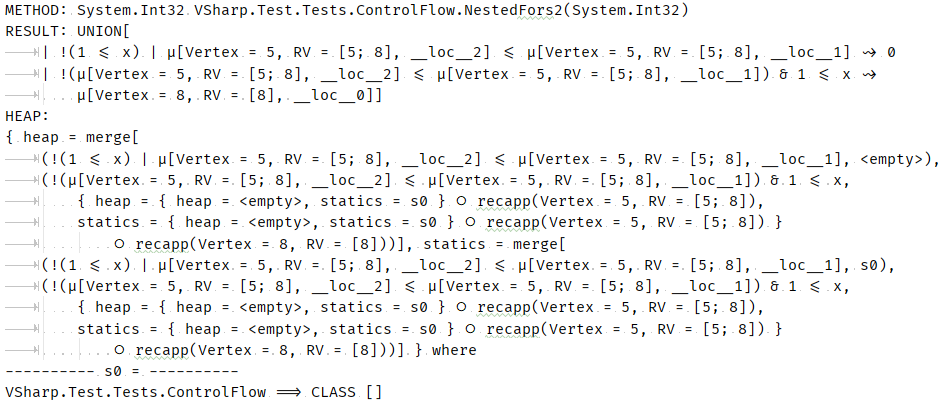
\includegraphics[scale=0.5]{Batoev/images/results.PNG}
\caption{Результат символьного исполнения метода~\ref{example:fors}}
\end{figure}

\begin{table}[t]
    \centering
    \begin{tabular}{ |p{3cm}||p{2cm}|p{2cm}|p{2cm}|  }
        \hline
        \multicolumn{4}{|c|}{Количественные характеристики тестов} \\
        \hline
        Название тестового набора &Количество тестов в наборе&Количество успешно пройденных тестов&Количество инструкций CIL\\
        \hline
        Arithmetics   &80    &77    &1968\\
        Logics        &75    &75    &1458\\
        Conditional   &10    &6     &943\\
        Recursive     &5     &5     &751\\
        Lambdas       &2     &2     &404\\
        Generic       &14    &14    &194\\
        Strings       &15    &15    &219\\
        Unsafe        &16    &16    &312\\
        Typecast      &19    &19    &969\\
        Methods       &10    &10    &238\\
        Lists         &9     &9     &1420\\
        Chess.NET     &1     &1     &2723\\
        \hline
        Всего         &256   &249   &11599\\
        \hline
    \end{tabular}
    \captionof{table}{Результаты тестирования}
    \label{experiments}
\end{table}


\FloatBarrier

\subsection{Тестирование интерпретатора}
Тестирование нового интерпретатора проводилось на тестовой подсистеме проекта <<VSharp.Test>> и на библиотеке \textsc{Chess.NET}.
Подсистема содержит тестовые наборы, затрагивающие различные конструкции и возможности языка C\#:
арифметику, логические операции,
работу с массивами разных размерностей, генерирование исключений, тесты на классы и структуры, включающие взаимодействие со статическими членами и вызовы виртуальных методов,
тесты с неограниченной рекурсией, тесты с \emph{unsafe}-кодом, тесты со строками. 

Таблица~\ref{experiments} показывает результаты проведенного тестирования. 
В наборах тестах с арифметикой и условными конструкциями была часть тестов с генерацией исключений. 
Поскольку схема обработки исключений для языка CIL не была реализована, то данные тесты были некорректно исполнены.
По той же причине не было проведено тестирования на тестовым наборе <<TryCatch>>, 
основное предназначение которого --- инициирование и перехват исключений.

\section{Заключение}

В данной работе описан подход к композициональному символьному исполнению без раскрутки. Была предложена концепция композициональной памяти с символьной адресацией. Был доказан некоторый набор свойств КСП, дающий основание для подхода в стиле систем переписывания, где символьные кучи могут сами выступать как символы. Это даёт возможность автоматически порождать уравнения на состояния, решения которых в точности отражают поведения функций, работающих с динамической памятью. Было показано как свести задачу решения уравнений на состояния к задаче проверки безопасности чистых функций второго порядка.

Данная работа нацелена на теоретические основания композиционального анализа динамической памяти. Мы оставляем апробацию этого подхода на будущее. Другим направлением будущих исследований может быть расширение нашего формализма на композициональный анализ параллельных программ.

\bibliographystyle{ugost2008ls}
\begin{thebibliography}{10}

\bibitem{baldoni2018survey}
Roberto Baldoni, Emilio Coppa, Daniele~Cono D’elia, Camil Demetrescu, and
  Irene Finocchi.
\newblock A survey of symbolic execution techniques.
\newblock {\em ACM Computing Surveys (CSUR)}, 51(3):50, 2018.

\bibitem{godefroid2007compositional}
Patrice Godefroid.
\newblock Compositional dynamic test generation.
\newblock In {\em ACM Sigplan Notices}, volume~42, pages 47--54. ACM, 2007.

\bibitem{jaffar2012tracer}
Joxan Jaffar, Vijayaraghavan Murali, Jorge~A Navas, and Andrew~E Santosa.
\newblock Tracer: A symbolic execution tool for verification.
\newblock In {\em International Conference on Computer Aided Verification},
  pages 758--766. Springer, 2012.

\bibitem{king1976symbolic}
James~C King.
\newblock Symbolic execution and program testing.
\newblock {\em Communications of the ACM}, 19(7):385--394, 1976.

\bibitem{kuznetsov2012efficient}
Volodymyr Kuznetsov, Johannes Kinder, Stefan Bucur, and George Candea.
\newblock Efficient state merging in symbolic execution.
\newblock {\em Acm Sigplan Notices}, 47(6):193--204, 2012.

\bibitem{mcmillan2010lazy}
Kenneth~L McMillan.
\newblock Lazy annotation for program testing and verification.
\newblock In {\em International Conference on Computer Aided Verification},
  pages 104--118. Springer, 2010.

\bibitem{kostyukov2018csewu}
Юрий~Олегович Костюков.
\newblock {\em Кучи как чистые функции:
  композициональное символьное исполнение
  без раскрутки}, pages 288--346.
\newblock 6. 2018.

\end{thebibliography}


\end{document}
